\documentclass[twoside]{book}

% Packages required by doxygen
\usepackage{fixltx2e}
\usepackage{calc}
\usepackage{doxygen}
\usepackage[export]{adjustbox} % also loads graphicx
\usepackage{graphicx}
\usepackage[utf8]{inputenc}
\usepackage{makeidx}
\usepackage{multicol}
\usepackage{multirow}
\PassOptionsToPackage{warn}{textcomp}
\usepackage{textcomp}
\usepackage[nointegrals]{wasysym}
\usepackage[table]{xcolor}

% Font selection
\usepackage[T1]{fontenc}
\usepackage[scaled=.90]{helvet}
\usepackage{courier}
\usepackage{amssymb}
\usepackage{sectsty}
\renewcommand{\familydefault}{\sfdefault}
\allsectionsfont{%
  \fontseries{bc}\selectfont%
  \color{darkgray}%
}
\renewcommand{\DoxyLabelFont}{%
  \fontseries{bc}\selectfont%
  \color{darkgray}%
}
\newcommand{\+}{\discretionary{\mbox{\scriptsize$\hookleftarrow$}}{}{}}

% Page & text layout
\usepackage{geometry}
\geometry{%
  a4paper,%
  top=2.5cm,%
  bottom=2.5cm,%
  left=2.5cm,%
  right=2.5cm%
}
\tolerance=750
\hfuzz=15pt
\hbadness=750
\setlength{\emergencystretch}{15pt}
\setlength{\parindent}{0cm}
\setlength{\parskip}{3ex plus 2ex minus 2ex}
\makeatletter
\renewcommand{\paragraph}{%
  \@startsection{paragraph}{4}{0ex}{-1.0ex}{1.0ex}{%
    \normalfont\normalsize\bfseries\SS@parafont%
  }%
}
\renewcommand{\subparagraph}{%
  \@startsection{subparagraph}{5}{0ex}{-1.0ex}{1.0ex}{%
    \normalfont\normalsize\bfseries\SS@subparafont%
  }%
}
\makeatother

% Headers & footers
\usepackage{fancyhdr}
\pagestyle{fancyplain}
\fancyhead[LE]{\fancyplain{}{\bfseries\thepage}}
\fancyhead[CE]{\fancyplain{}{}}
\fancyhead[RE]{\fancyplain{}{\bfseries\leftmark}}
\fancyhead[LO]{\fancyplain{}{\bfseries\rightmark}}
\fancyhead[CO]{\fancyplain{}{}}
\fancyhead[RO]{\fancyplain{}{\bfseries\thepage}}
\fancyfoot[LE]{\fancyplain{}{}}
\fancyfoot[CE]{\fancyplain{}{}}
\fancyfoot[RE]{\fancyplain{}{\bfseries\scriptsize Generated by Doxygen }}
\fancyfoot[LO]{\fancyplain{}{\bfseries\scriptsize Generated by Doxygen }}
\fancyfoot[CO]{\fancyplain{}{}}
\fancyfoot[RO]{\fancyplain{}{}}
\renewcommand{\footrulewidth}{0.4pt}
\renewcommand{\chaptermark}[1]{%
  \markboth{#1}{}%
}
\renewcommand{\sectionmark}[1]{%
  \markright{\thesection\ #1}%
}

% Indices & bibliography
\usepackage{natbib}
\usepackage[titles]{tocloft}
\setcounter{tocdepth}{3}
\setcounter{secnumdepth}{5}
\makeindex

% Hyperlinks (required, but should be loaded last)
\usepackage{ifpdf}
\ifpdf
  \usepackage[pdftex,pagebackref=true]{hyperref}
\else
  \usepackage[ps2pdf,pagebackref=true]{hyperref}
\fi
\hypersetup{%
  colorlinks=true,%
  linkcolor=blue,%
  citecolor=blue,%
  unicode%
}

% Custom commands
\newcommand{\clearemptydoublepage}{%
  \newpage{\pagestyle{empty}\cleardoublepage}%
}

\usepackage{caption}
\captionsetup{labelsep=space,justification=centering,font={bf},singlelinecheck=off,skip=4pt,position=top}

%===== C O N T E N T S =====

\begin{document}

% Titlepage & ToC
\hypersetup{pageanchor=false,
             bookmarksnumbered=true,
             pdfencoding=unicode
            }
\pagenumbering{alph}
\begin{titlepage}
\vspace*{7cm}
\begin{center}%
{\Large Fast Image \\[1ex]\large 1.\+0.\+8 }\\
\vspace*{1cm}
{\large Generated by Doxygen 1.8.13}\\
\end{center}
\end{titlepage}
\clearemptydoublepage
\pagenumbering{roman}
\tableofcontents
\clearemptydoublepage
\pagenumbering{arabic}
\hypersetup{pageanchor=true}

%--- Begin generated contents ---
\chapter{Fast Image (FI) \+: A High-\/\+Performance Accessor for Processing Gigapixel Images}
\label{index}\hypertarget{index}{}An application programming interface to access big images

The A\+PI is designed to aid in creating image processing algorithms to obtain performance across C\+P\+Us and big images.

\subsection*{Content}


\begin{DoxyItemize}
\item \href{#installation-instructions}{\tt Installation Instructions}
\begin{DoxyItemize}
\item \href{#dependencies}{\tt Dependencies}
\item \href{#building-fast-image}{\tt Building Fast Image}
\end{DoxyItemize}
\item \href{#motivation}{\tt Motivation}
\item \href{#approach}{\tt Approach}
\item \href{#architecture}{\tt Architecture}
\item \href{#steps-to-programming-with-fast-image}{\tt Steps to Programming with Fast Image}
\begin{DoxyItemize}
\item \href{#linking-_fast-image_}{\tt Linking Fast Image}
\item \href{#api-overview}{\tt A\+PI overview}
\item \href{#how-to-create-a-tile-loader-how-to-access-a-specific-file-}{\tt How to create a Tile Loader ? How to access a specific file ?}
\item \href{#getting-started}{\tt Getting started}
\begin{DoxyItemize}
\item \href{#image-traversal}{\tt Image traversal}
\item \href{#spatial-convolution}{\tt Spatial convolution}
\item \href{#opencv-convolution}{\tt Open\+CV convolution}
\item \href{#feature-collection-usage}{\tt Feature Collection usage}
\end{DoxyItemize}
\end{DoxyItemize}
\item \href{#credits}{\tt Credits}
\item \href{#contact-us}{\tt Contact Us}
\end{DoxyItemize}

\section*{Installation Instructions}

\subsection*{Dependencies}

1) g++/gcc version 4.\+8.\+4+

2) H\+T\+GS (\href{https://github.com/usnistgov/htgs}{\tt https\+://github.\+com/usnistgov/htgs})

3) Lib\+T\+I\+FF (\href{http://www.simplesystems.org/libtiff/}{\tt http\+://www.\+simplesystems.\+org/libtiff/}) \mbox{[}optional / Tile\+Loader\mbox{]}

4) libpng (\href{http://www.libpng.org/}{\tt http\+://www.\+libpng.\+org/}) \mbox{[}optional / Tile\+Loader\mbox{]}

5) doxygen (www.\+doxygen.\+org/) \mbox{[}optional / Documentation\mbox{]}

\subsection*{Building Fast Image}

{\bfseries C\+Make Options\+:}

C\+M\+A\+K\+E\+\_\+\+I\+N\+S\+T\+A\+L\+L\+\_\+\+P\+R\+E\+F\+IX -\/ Where to install Fast Image (and documentation)

B\+U\+I\+L\+D\+\_\+\+D\+O\+X\+Y\+G\+EN -\/ Creates doxygen documentation

R\+U\+N\+\_\+\+G\+T\+E\+ST -\/ Compiles and runs google unit tests for Fast Image (\textquotesingle{}make run-\/test\textquotesingle{} to re-\/run)


\begin{DoxyCode}
:$ cd <FastImage\_Directory>
:<FastImage\_Directory>$ mkdir build && cd build
:<FastImage\_Directory>/build$ ccmake ../ (or cmake-gui)

'Configure' and setup cmake parameters
'Configure' and 'Build'

:<FastImage\_Directory>/build$ make
:<FastImage\_Directory>/build$ [sudo] make install
\end{DoxyCode}


\section*{Motivation}

The hardware landscape for high-\/performance computing currently features compute nodes with a high degree of parallelism within a node (e.\+g., 46 cores for the newly-\/announced Qualcomm Centriq C\+PU, 32 physical cores for the A\+MD Epyc C\+PU, and 24 logical cores for an Intel Xeon Skylake C\+PU), that increases with every new hardware generation. By contrast, the amount of memory available per core is not increasing in a commensurate manner and may even be decreasing especially when considered on a per-\/core basis. Furthermore, while the computational capacity of these systems keeps on improving, their programmability remains quite challenging. As such, designing image processing algorithms to minimize memory usage is a key strategy to taking advantage of this parallelism and support concurrent users or the multi-\/threaded processing to large images.

\section*{Approach}

{\itshape Fast Image} improves programmer productivity by providing high-\/level abstractions, {\itshape View} and {\itshape Tile}, along with routines that build on these abstractions to operate across an entire image without actually loading it in memory. The library operates on tiles (e.\+g., a 1024x1024 partial image out of a very large 100K x 100K image) with possibly a halo of pixels around an individual tile. {\itshape Fast Image} only loads a small number of tiles to maintain a low-\/memory footprint and manages an in-\/memory cache. Furthermore, the library takes advantage of multi-\/core computing by offloading tiles to compute threads as soon as they become available. This allows for multiple users to maintain high throughput, while processing several images or views concurrently.

\section*{Architecture}

{\itshape Fast Image} architecture shows how the system work and interact with the algorithm. First of all it works asynchronously from the algorithm. Secondly each part of Fast Image will be on on different threads. Finally the static memory manager guaranty that the amount of memory will be limited as asked.

When an algorithm will ask {\itshape n} views through {\itshape View Request}. {\itshape Fast Image} will use this {\itshape View Request} to build a {\itshape view} and make it available as soon as possible. The algorithm will be able to use it (and release it). In the mean time, if enough memory is available an other {\itshape view} will be created.

The {\itshape View} creation go through 3 steps\+:
\begin{DoxyEnumerate}
\item {\itshape View Loader}\+: Request memory from the memory manager and split the {\itshape View Request}, to {\itshape n} {\itshape Tile Loader} and send them to the {\itshape Tile Loader}.
\item {\itshape Tile Loader}\+: Specific to the file {\itshape Fast Image} access to. Will ask the {\itshape Tile} to {\itshape Tile Cache}, if it not available the {\itshape Tile} will be loaded from the file, then cast and copy to the {\itshape Tile Cache}. From the cache only the interesting {\itshape Tile}\textquotesingle{}s part will be copied to the {\itshape View}.
\item {\itshape View Counter}\+: Wait to the {\itshape view} to be fully loaded from file\textquotesingle{}s parts. Then build the ghost region if needed, and send the complete {\itshape view} to the algorithm.
\end{DoxyEnumerate}

Following the Fast Image Graph and it\textquotesingle{}s interaction with the algorithm\+:

 \section*{Steps to Programming with Fast Image}

\subsection*{Linking {\itshape Fast Image}}

{\itshape Fast Image} can be easily link to any C++ 11 compliant code using cmake. Add the path to the folder Fast\+Image\+Directory/cmake-\/modules/ to the C\+M\+A\+K\+E\+\_\+\+M\+O\+D\+U\+L\+E\+\_\+\+P\+A\+TH variable in your C\+Make\+Lists.\+txt. Then add the following lines in your C\+Make\+Lists.\+txt\+: 
\begin{DoxyCode}
find\_package(FastImage REQUIRED)
include\_directories($\{HTGS\_INCLUDE\_DIR\})
include\_directories($\{FastImage\_INCLUDE\_DIR\})
link\_libraries($\{FastImage\_LIBRARIES\})
\end{DoxyCode}


\subsection*{A\+PI overview}

3 A\+PI exists in {\itshape Fast Image}\+:
\begin{DoxyEnumerate}
\item The Fast\+Image object to access views of an image
\item The {\itshape View} object to access pixel/data in the {\itshape View}
\item Feature\+Collection to get the information on region of interests
\item Tile Loader
\end{DoxyEnumerate}

\subsection*{How to create a Tile Loader ? How to access a specific file ?}

To access to a new file format, a specific {\itshape Tile Loader} is needed. A specific {\itshape Tile Loader} class will inherit from the class {\itshape A\+Tile\+Loader}.

The following methods need to be implemented\+: 
\begin{DoxyCode}
\textcolor{comment}{// Constructor}
ATileLoader                       (\textcolor{keyword}{const} std::string &filePath, \textcolor{keywordtype}{size\_t} numThreads = 1);

\textcolor{comment}{// Copy function to duplicate the Tile Loader into n threads }
ATileLoader*  copyTileLoader      ();

\textcolor{comment}{// Task Name getter used for graph generation }
std::string   getName             ();

\textcolor{comment}{// Basic file information getter }
uint32\_t      getImageHeight      (uint32\_t level = 0) \textcolor{keyword}{const};
uint32\_t      getImageWidth       (uint32\_t level = 0) \textcolor{keyword}{const};
uint32\_t      getTileWidth        (uint32\_t level = 0) \textcolor{keyword}{const};
uint32\_t      getTileHeight       (uint32\_t level = 0) \textcolor{keyword}{const};
\textcolor{keywordtype}{short}         getBitsPerSample    () \textcolor{keyword}{const};
uint32\_t      getNbPyramidLevels  () \textcolor{keyword}{const};

\textcolor{comment}{// Load a specific tile from the file, the tile has already allocated. Return the disk loading time in ms.}
\textcolor{keywordtype}{double}        loadTileFromFile    (UserType *tile, uint32\_t indexRowGlobalTile, uint32\_t indexColGlobalTile
      );
\end{DoxyCode}


Here a Tile Loader for Greyscale Tiled Tiff\+:


\begin{DoxyCode}
\textcolor{keyword}{template}<\textcolor{keyword}{typename} UserType>
\textcolor{keyword}{class }TiffTileLoader : \textcolor{keyword}{public} ATileLoader<UserType> \{
 \textcolor{keyword}{private}:
  TIFF *
      \_tiff = \textcolor{keyword}{nullptr};

  uint32\_t
      \_imageHeight = 0,
      \_imageWidth = 0,
      \_tileHeight = 0,
      \_tileWidth = 0;

  \textcolor{keywordtype}{short}
      \_sampleFormat = 0,
      \_bitsPerSample = 0;

  \textcolor{comment}{// Copy Constructor used by copyTileLoader}
  TiffTileLoader(\textcolor{keywordtype}{size\_t} numThreads, \textcolor{keyword}{const} std::string &filePath, \textcolor{keyword}{const} TiffTileLoader &from)
      : ATileLoader<UserType>(filePath, numThreads) \{
    this->\_tiff = TIFFOpen(filePath.c\_str(), \textcolor{stringliteral}{"r"});
    this->\_imageWidth = from.\_imageWidth;
    this->\_imageHeight = from.\_imageHeight;
    this->\_tileWidth = from.\_tileWidth;
    this->\_tileHeight = from.\_tileHeight;
    this->\_bitsPerSample = from.\_bitsPerSample;
    this->\_sampleFormat = from.\_sampleFormat;
  \}

 \textcolor{keyword}{public}:
  \textcolor{comment}{// Tile Loader constructor where the actual file is open}
  TiffTileLoader(\textcolor{keyword}{const} std::string &fileName, \textcolor{keywordtype}{size\_t} numThreads = 1) : ATileLoader<UserType>(fileName,
                                                                                             numThreads) \{
    \textcolor{keywordtype}{short} samplesPerPixel = 0;

    this->\_tiff = TIFFOpen(fileName.c\_str(), \textcolor{stringliteral}{"r"});
    \textcolor{keywordflow}{if} (this->\_tiff != \textcolor{keyword}{nullptr}) \{
      \textcolor{keywordflow}{if} (TIFFIsTiled(\_tiff) == 0) \{
        std::stringstream message;
        message << \textcolor{stringliteral}{"Tile Loader ERROR: The image is not tiled."};
        \textcolor{keyword}{auto} messageChr = \textcolor{keyword}{new} \textcolor{keywordtype}{char}[message.str().length() + 1];
        strcpy(messageChr, message.str().c\_str());
        \textcolor{keywordflow}{throw} (FastImageException(messageChr));
      \}
      TIFFGetField(this->\_tiff, TIFFTAG\_IMAGEWIDTH, &(this->\_imageWidth));
      TIFFGetField(this->\_tiff, TIFFTAG\_IMAGELENGTH, &(this->\_imageHeight));
      TIFFGetField(this->\_tiff, TIFFTAG\_TILEWIDTH, &this->\_tileWidth);
      TIFFGetField(this->\_tiff, TIFFTAG\_TILELENGTH, &this->\_tileHeight);
      TIFFGetField(this->\_tiff, TIFFTAG\_SAMPLESPERPIXEL, &samplesPerPixel);
      TIFFGetField(this->\_tiff, TIFFTAG\_BITSPERSAMPLE, &(this->\_bitsPerSample));
      TIFFGetField(this->\_tiff, TIFFTAG\_SAMPLEFORMAT, &(this->\_sampleFormat));

      \textcolor{keywordflow}{if} (samplesPerPixel != 1) \{
        std::stringstream message;
        message << \textcolor{stringliteral}{"Tile Loader ERROR: The image is not greyscale: SamplesPerPixel = "} << samplesPerPixel
                << \textcolor{stringliteral}{"."};
        \textcolor{keyword}{auto} messageChr = \textcolor{keyword}{new} \textcolor{keywordtype}{char}[message.str().length() + 1];
        strcpy(messageChr, message.str().c\_str());
        \textcolor{keywordflow}{throw} (FastImageException(messageChr));
      \}

      \textcolor{keywordflow}{if} (\_sampleFormat < 1 && \_sampleFormat > 3) \{
        \_sampleFormat = 1;
      \}

    \} \textcolor{keywordflow}{else} \{
      std::stringstream message;
      message << \textcolor{stringliteral}{"Tile Loader ERROR: The image can not be opened."};
      \textcolor{keyword}{auto} messageChr = \textcolor{keyword}{new} \textcolor{keywordtype}{char}[message.str().length() + 1];
      strcpy(messageChr, message.str().c\_str());
      \textcolor{keywordflow}{throw} (FastImageException(messageChr));
    \}
  \}

  ~TiffTileLoader() \{
    \textcolor{keywordflow}{if} (this->\_tiff != \textcolor{keyword}{nullptr}) \{
      TIFFClose(this->\_tiff);
    \}
  \}

  \textcolor{comment}{// Differents getter specific to the file format}
  std::string getName()\textcolor{keyword}{ override }\{ \textcolor{keywordflow}{return} \textcolor{stringliteral}{"TIFF Tile Loader"}; \}
  uint32\_t getImageHeight(uint32\_t level = 0)\textcolor{keyword}{ const override }\{ \textcolor{keywordflow}{return} \_imageHeight; \}
  uint32\_t getImageWidth(uint32\_t level = 0)\textcolor{keyword}{ const override }\{ \textcolor{keywordflow}{return} \_imageWidth; \}
  uint32\_t getTileWidth(uint32\_t level = 0)\textcolor{keyword}{ const override }\{ \textcolor{keywordflow}{return} \_tileWidth; \}
  uint32\_t getTileHeight(uint32\_t level = 0)\textcolor{keyword}{ const override }\{ \textcolor{keywordflow}{return} \_tileHeight; \}
  \textcolor{keywordtype}{short} getBitsPerSample()\textcolor{keyword}{ const override }\{ \textcolor{keywordflow}{return} \_bitsPerSample; \}
  uint32\_t getNbPyramidLevels()\textcolor{keyword}{ const override }\{ \textcolor{keywordflow}{return} 1; \}

  \textcolor{keyword}{template}<\textcolor{keyword}{typename} FileType>
  \textcolor{keywordtype}{void} loadTile(tdata\_t src, UserType *dest) \{
    \textcolor{keywordflow}{for} (uint32\_t row = 0; row < \_tileHeight; ++row) \{
      \textcolor{keywordflow}{for} (uint32\_t col = 0; col < \_tileWidth; ++col) \{
        dest[row * \_tileWidth + col] = (UserType) ((FileType *) (src))[row * \_tileWidth + col];
      \}
    \}
  \}

  \textcolor{comment}{// Load the tile from the file }
  \textcolor{keywordtype}{double} loadTileFromFile(UserType *tile, uint32\_t indexRowGlobalTile, uint32\_t indexColGlobalTile)\textcolor{keyword}{
       override }\{
    tdata\_t tiffTile = \textcolor{keyword}{nullptr};
    tiffTile = \_TIFFmalloc(TIFFTileSize(\_tiff));
    \textcolor{keyword}{auto} begin = std::chrono::high\_resolution\_clock::now();
    TIFFReadTile(\_tiff, tiffTile, indexColGlobalTile * \_tileWidth, indexRowGlobalTile * \_tileHeight, 0, 0);
    \textcolor{keyword}{auto} end = std::chrono::high\_resolution\_clock::now();
    \textcolor{keywordtype}{double} diskDuration = (std::chrono::duration\_cast<std::chrono::nanoseconds>(end - begin).count());
    std::stringstream message;
    \textcolor{keywordflow}{switch} (this->\_sampleFormat) \{
      \textcolor{keywordflow}{case} 1 :
        \textcolor{keywordflow}{switch} (this->\_bitsPerSample) \{
          \textcolor{keywordflow}{case} 8:loadTile<uint8\_t>(tiffTile, tile);
            \textcolor{keywordflow}{break};
          \textcolor{keywordflow}{case} 16:loadTile<uint16\_t>(tiffTile, tile);
            \textcolor{keywordflow}{break};
          \textcolor{keywordflow}{case} 32:loadTile<uint32\_t>(tiffTile, tile);
            \textcolor{keywordflow}{break};
          \textcolor{keywordflow}{case} 64:loadTile<uint64\_t>(tiffTile, tile);
            \textcolor{keywordflow}{break};
          \textcolor{keywordflow}{default}:
            message << \textcolor{stringliteral}{"Tile Loader ERROR: The data format is not supported for unsigned integer, "}
                \textcolor{stringliteral}{"number bits per pixel = "} << this->\_bitsPerSample;
            \textcolor{keyword}{auto} messageChr = \textcolor{keyword}{new} \textcolor{keywordtype}{char}[message.str().length() + 1];
            strcpy(messageChr, message.str().c\_str());
            \textcolor{keywordflow}{throw} (FastImageException(messageChr));
        \}
        \textcolor{keywordflow}{break};
      \textcolor{keywordflow}{case} 2:
        \textcolor{keywordflow}{switch} (this->\_bitsPerSample) \{
          \textcolor{keywordflow}{case} 8:loadTile<int8\_t>(tiffTile, tile);
            \textcolor{keywordflow}{break};
          \textcolor{keywordflow}{case} 16:loadTile<int16\_t>(tiffTile, tile);
            \textcolor{keywordflow}{break};
          \textcolor{keywordflow}{case} 32:loadTile<int32\_t>(tiffTile, tile);
            \textcolor{keywordflow}{break};
          \textcolor{keywordflow}{case} 64:loadTile<int64\_t>(tiffTile, tile);
            \textcolor{keywordflow}{break};
          \textcolor{keywordflow}{default}:
            message << \textcolor{stringliteral}{"Tile Loader ERROR: The data format is not supported for signed integer, "}
                \textcolor{stringliteral}{"number bits per pixel = "} << this->\_bitsPerSample;
            \textcolor{keyword}{auto} messageChr = \textcolor{keyword}{new} \textcolor{keywordtype}{char}[message.str().length() + 1];
            strcpy(messageChr, message.str().c\_str());
            \textcolor{keywordflow}{throw} (FastImageException(messageChr));
        \}
        \textcolor{keywordflow}{break};
      \textcolor{keywordflow}{case} 3:
        \textcolor{keywordflow}{switch} (this->\_bitsPerSample) \{
          \textcolor{keywordflow}{case} 8:loadTile<float>(tiffTile, tile);
            \textcolor{keywordflow}{break};
          \textcolor{keywordflow}{case} 16:loadTile<float>(tiffTile, tile);
            \textcolor{keywordflow}{break};
          \textcolor{keywordflow}{case} 32:loadTile<float>(tiffTile, tile);
            \textcolor{keywordflow}{break};
          \textcolor{keywordflow}{case} 64:loadTile<double>(tiffTile, tile);
            \textcolor{keywordflow}{break};
          \textcolor{keywordflow}{default}:
            message << \textcolor{stringliteral}{"Tile Loader ERROR: The data format is not supported for float, "}
                \textcolor{stringliteral}{"number bits per pixel = "} << this->\_bitsPerSample;
            \textcolor{keyword}{auto} messageChr = \textcolor{keyword}{new} \textcolor{keywordtype}{char}[message.str().length() + 1];
            strcpy(messageChr, message.str().c\_str());
            \textcolor{keywordflow}{throw} (FastImageException(messageChr));
        \}
        \textcolor{keywordflow}{break};
      \textcolor{keywordflow}{default}:
        message << \textcolor{stringliteral}{"Tile Loader ERROR: The data format is not supported, sample format = "}
                << this->\_sampleFormat;
        \textcolor{keyword}{auto} messageChr = \textcolor{keyword}{new} \textcolor{keywordtype}{char}[message.str().length() + 1];
        strcpy(messageChr, message.str().c\_str());
        \textcolor{keywordflow}{throw} (FastImageException(messageChr));
    \}
    \_TIFFfree(tiffTile);
    \textcolor{keywordflow}{return} diskDuration;
  \}

  \textcolor{comment}{// Copy the Tile Loader}
  ATileLoader<UserType> *copyTileLoader()\textcolor{keyword}{ override }\{
    \textcolor{keywordflow}{return} \textcolor{keyword}{new} TiffTileLoader<UserType>(this->getNumThreads(), this->getFilePath(), *\textcolor{keyword}{this});
  \}
\};
\}
\end{DoxyCode}


\#\# Getting started 
\begin{DoxyCode}
The code in this section is only PSEUDOCODE, and is not meant to be executed as is.
\end{DoxyCode}


\subsubsection*{Image traversal}

Here a little program to go through all the pixel in a tiled greyscale tiff image\+: 
\begin{DoxyCode}
\textcolor{comment}{// Tile loader creation depending on the image}
\hyperlink{classfi_1_1ATileLoader}{fi::ATileLoader<uint32\_t>} *tileLoader = \textcolor{keyword}{new} fi::TiffTileLoader<uint32\_t>(pathImage
      ); 

\textcolor{comment}{// Fast Image accessor creation}
\textcolor{keyword}{auto} *fi = \textcolor{keyword}{new} \hyperlink{classfi_1_1FastImage}{fi::FastImage<uint32\_t>}(tileLoader, 0);

\textcolor{comment}{// Configure and run the Fast Image}
fi->\hyperlink{classfi_1_1FastImage_aa2ae5e5498f57462abd876108a55475c}{configureAndRun}();

\textcolor{comment}{// Requesting all tiles }
fi->requestAllTiles(\textcolor{keyword}{true});

\textcolor{comment}{// Getting Data while Fast Image is processing some}
\textcolor{keywordflow}{while} (fi->isGraphProcessingTiles()) \{

    \textcolor{comment}{// Getting an image's view }
    \textcolor{keyword}{auto} pView = fi->getAvailableViewBlocking();

    \textcolor{comment}{// If not the last one}
    \textcolor{keywordflow}{if} (pView != \textcolor{keyword}{nullptr}) \{

        \textcolor{comment}{// Resolve shared\_ptr}
        \textcolor{keyword}{auto} view = pView->get();
        \textcolor{comment}{// Get information on the tile and looping through it }
        \textcolor{keywordflow}{for} (int32\_t r = 0; r < view->getTileHeight(); ++r) \{
            \textcolor{keywordflow}{for} (int32\_t c = 0; c < view->getTileWidth(); ++c) \{
                \textcolor{comment}{// Getting the pixel}
                view->getPixel(r, c);
            \}
        \}

        \textcolor{comment}{// Release the memory}
        pView->releaseMemory();
    \}
\}

\textcolor{comment}{// Waiting for FI to copmlete all it tasks}
fi->waitForGraphComplete();

\textcolor{comment}{// Delete Fast Image (it will take care of the Tile Loader)}
\textcolor{keyword}{delete} fi;
\end{DoxyCode}


\subsubsection*{Spatial convolution}

This code do a spatial convolution on a tiled greyscale tiff image (kernel creation and tile writing are not showed). A full example is given in the fast image example. 
\begin{DoxyCode}
\textcolor{keywordtype}{int} radius = 6;
\textcolor{keywordtype}{float} pixelOut = 0;
\textcolor{keywordtype}{double} sigma = 2;
int32\_t sizeKernel = radius * 2 + 1;


\hyperlink{classfi_1_1ATileLoader}{fi::ATileLoader<uint32\_t>} *tileLoader = \textcolor{keyword}{new} fi::TiffTileLoader<uint32\_t>(pathImage
      ); \textcolor{comment}{// Tile loader creation depending on the image}
\textcolor{keyword}{auto} *fi = \textcolor{keyword}{new} \hyperlink{classfi_1_1FastImage}{fi::FastImage<uint32\_t>}(tileLoader, 0); \textcolor{comment}{// Fast Image accessor
       creation}

std::vector<double> kernel = gaussian(radiusKernel, sigma); \textcolor{comment}{// Kernel creation }
\textcolor{keyword}{auto} *tileOut = \textcolor{keyword}{new} \textcolor{keywordtype}{float}[fi->getTileWidth() * fi->getTileHeight()]();

fi->configureAndRun(); \textcolor{comment}{// Configure and run the Fast Image}
fi->requestAllTiles(\textcolor{keyword}{true}); \textcolor{comment}{// Requesting all tiles }

\textcolor{comment}{// Getting Data while Fast Image is processing some}
\textcolor{keywordflow}{while} (fi->isGraphProcessingTiles()) \{
    \textcolor{keyword}{auto} pView = fi->getAvailableViewBlocking(); \textcolor{comment}{// Getting an image's view }
    \textcolor{comment}{// If not the last one}
    \textcolor{keywordflow}{if} (pView != \textcolor{keyword}{nullptr}) \{

        \textcolor{keyword}{auto} view = pView->get(); \textcolor{comment}{// Resolve shared\_ptr}
        \textcolor{comment}{// Get information on the tile and looping through it }
        \textcolor{keywordflow}{for} (int32\_t r = 0; r < view->getTileHeight(); ++r) \{
            \textcolor{keywordflow}{for} (int32\_t c = 0; c < view->getTileWidth(); ++c) \{
                pixelOut = 0;
                \textcolor{keywordflow}{for} (int32\_t rK = -radius; rK <= radius; ++rK) \{
                    \textcolor{keywordflow}{for} (int32\_t cK = -radius; cK <= radius; ++cK) \{
                        pixelOut += view->getPixel(r + rK, c + cK) * kernel[(rK + radius) * sizeKernel + (
      cK + radius)];
                    \}
                \}
                tileOut[r * tileWidth + c] = pixelOut / (view->getTileHeight() * view->getTileWidth());
            \}
        \}

        writeTile(tileOut, view->getGlobalXOffset(), view->getGlobalYOffset());
        \textcolor{comment}{// Release the memory}
        pView->releaseMemory();
    \}
\}

\textcolor{keyword}{delete} [] tileOut;
\textcolor{keyword}{delete} (fi)
\end{DoxyCode}


\subsubsection*{Open\+CV convolution}

This code do a convolution with Open\+CV on a tiled greyscale tiff image (kernel creation and tile writing are not showed). A full example is given in the fast image example. 
\begin{DoxyCode}
\textcolor{keyword}{using namespace }cv; 

\textcolor{keywordtype}{int} radius = 6;
\textcolor{keywordtype}{float} pixelOut = 0;
\textcolor{keywordtype}{double} sigma = 2;
int32\_t sizeKernel = radius * 2 + 1;


\hyperlink{classfi_1_1ATileLoader}{fi::ATileLoader<uint32\_t>} *tileLoader = \textcolor{keyword}{new} fi::TiffTileLoader<uint32\_t>(pathImage
      ); \textcolor{comment}{// Tile loader creation depending on the image}
\textcolor{keyword}{auto} *fi = \textcolor{keyword}{new} \hyperlink{classfi_1_1FastImage}{fi::FastImage<uint32\_t>}(tileLoader, 0); \textcolor{comment}{// Fast Image accessor
       creation}

Mat kernel = gaussian(radius, sigma, CV\_32F); \textcolor{comment}{// Kernel creation }

\textcolor{keyword}{auto} *tileOut = \textcolor{keyword}{new} \textcolor{keywordtype}{float}[fi->getTileWidth() * fi->getTileHeight()]();

fi->configureAndRun(); \textcolor{comment}{// Configure and run the Fast Image}
fi->requestAllTiles(\textcolor{keyword}{true}); \textcolor{comment}{// Requesting all tiles }

\textcolor{keyword}{auto} viewHeight = fi->getViewHeight();
\textcolor{keyword}{auto} viewWidth = fi->getViewWidth();

\textcolor{comment}{// Getting Data while Fast Image is processing some}
\textcolor{keywordflow}{while} (fi->isGraphProcessingTiles()) \{
    \textcolor{keyword}{auto} pView = fi->getAvailableViewBlocking(); \textcolor{comment}{// Getting an image's view }
    \textcolor{comment}{// If not the last one}
    \textcolor{keywordflow}{if} (pView != \textcolor{keyword}{nullptr}) \{
        \textcolor{keyword}{auto} view = pView->get(); \textcolor{comment}{// Resolve shared\_ptr}

        Mat matInput(viewHeight, viewWidth, CV\_32F, view->getData())
        Mat tileResult;

        \textcolor{comment}{//Do the convolution}
        filter2D(matInput, tileResult, CV\_32F, \_kernel, cvPoint(-1, -1));

        cv::Rect roi(radius, radius, view->getTileWidth(), view->getTileHeight());
        cv::Mat<float> matOut = tileResult(roi).clone();

        tileOut = (\textcolor{keywordtype}{float} *)matOut.data;

        writeTile(tileOut, view->getGlobalXOffset(), view->getGlobalYOffset());
        \textcolor{comment}{// Release the memory}
        pView->releaseMemory();
    \}
\}

\textcolor{keyword}{delete} [] tileOut;
\textcolor{keyword}{delete} (fi)
\end{DoxyCode}


\subsubsection*{Feature Collection usage}

This code go through a tiled greyscale tiff image (kernel creation and tile writing are not showed) through is mask. A full example is given in the fast image example. 
\begin{DoxyCode}
\hyperlink{classfi_1_1ATileLoader}{fi::ATileLoader<uint32\_t>} *tileLoader = \textcolor{keyword}{new} fi::TiffTileLoader<uint32\_t>(pathImage
      ); \textcolor{comment}{// Tile loader creation depending on the image}
\textcolor{keyword}{auto} *fi = \textcolor{keyword}{new} \hyperlink{classfi_1_1FastImage}{fi::FastImage<uint32\_t>}(tileLoader, 0); \textcolor{comment}{// Fast Image accessor
       creation}

\textcolor{comment}{// Feature Collection creation }
\hyperlink{classfc_1_1FeatureCollection}{fc::FeatureCollection} featureCollection;
featureCollection.deserialize(pathFeatureCollection);

fi->\hyperlink{classfi_1_1FastImage_aa2ae5e5498f57462abd876108a55475c}{configureAndRun}();

\textcolor{comment}{// Go through all features}
\textcolor{keywordflow}{for} (\textcolor{keyword}{const} \textcolor{keyword}{auto} &feature : featureCollection) \{
    \textcolor{comment}{// Request views from a feature}
    fi->requestFeature(feature);
    \textcolor{keywordflow}{while} (!fi->isFeatureDone()) \{
        \textcolor{keyword}{auto} sh\_view = fi->getAvailableViewBlocking();
        \textcolor{keyword}{auto} view = sh\_view->get();
        \textcolor{keywordflow}{if} (view != \textcolor{keyword}{nullptr}) \{
            \textcolor{keywordflow}{for} (\textcolor{keyword}{auto} row = 0; row < view->getTileHeight(); ++row) \{
                \textcolor{keywordflow}{for} (\textcolor{keyword}{auto} col = 0; col < view->getTileWidth(); ++col) \{

                    \textcolor{comment}{// Test is a pixel is in the bitmask}
                    \textcolor{keywordflow}{if} (feature.isInBitMask(row + view->getGlobalYOffset(), col + view->getGlobalXOffset())
      ) \{
                        view->getPixel(row, col);
                    \}

                \}
            \}
            sh\_view->releaseMemory();
        \}
    \}
\}
fi->finishedRequestingTiles();
\textcolor{keyword}{delete} fi;
\end{DoxyCode}


\section*{Credits}

Alexandre Bardakoff

Timothy Blattner

Walid Keyrouz

Mary Brady

\section*{Contact Us}

\href{mailto:alexandre.bardakoff@nist.gov}{\tt Alexandre Bardakoff (alexandre.\+bardakoff ( at ) nist.\+gov}

\href{mailto:timothy.blattner@nist.gov}{\tt Timothy Blattner (timothy.\+blattner ( at ) nist.\+gov} 
\chapter{Namespace Index}
\section{Namespace List}
Here is a list of all namespaces with brief descriptions\+:\begin{DoxyCompactList}
\item\contentsline{section}{\hyperlink{namespacefc}{fc} \\*\hyperlink{classfc_1_1FeatureCollection}{Feature\+Collection} namespace }{\pageref{namespacefc}}{}
\item\contentsline{section}{\hyperlink{namespacefi}{fi} \\*\hyperlink{classfi_1_1FastImage}{Fast\+Image} namespace }{\pageref{namespacefi}}{}
\end{DoxyCompactList}

\chapter{Hierarchical Index}
\section{Class Hierarchy}
This inheritance list is sorted roughly, but not completely, alphabetically\+:\begin{DoxyCompactList}
\item \contentsline{section}{fc\+:\+:A\+A\+B\+B\+Tree$<$ ObjectT $>$\+:\+:A\+A\+B\+B\+Node}{\pageref{structfc_1_1AABBTree_1_1AABBNode}}{}
\item \contentsline{section}{fc\+:\+:A\+A\+B\+B\+Tree$<$ ObjectT $>$}{\pageref{classfc_1_1AABBTree}}{}
\item \contentsline{section}{fc\+:\+:A\+A\+B\+B\+Tree$<$ fc\+:\+:Feature $>$}{\pageref{classfc_1_1AABBTree}}{}
\item \contentsline{section}{fc\+:\+:Blob}{\pageref{classfc_1_1Blob}}{}
\item \contentsline{section}{fc\+:\+:Bounding\+Box}{\pageref{classfc_1_1BoundingBox}}{}
\item \contentsline{section}{fi\+:\+:Cached\+Tile$<$ User\+Type $>$}{\pageref{classfi_1_1CachedTile}}{}
\item \contentsline{section}{fc\+:\+:Cuboid$<$ T $>$}{\pageref{classfc_1_1Cuboid}}{}
\item \contentsline{section}{fc\+:\+:Cuboid$<$ double $>$}{\pageref{classfc_1_1Cuboid}}{}
\item std\+:\+:exception\begin{DoxyCompactList}
\item \contentsline{section}{fi\+:\+:Fast\+Image\+Exception}{\pageref{classfi_1_1FastImageException}}{}
\end{DoxyCompactList}
\item \contentsline{section}{fi\+:\+:Fast\+Image$<$ User\+Type $>$}{\pageref{classfi_1_1FastImage}}{}
\item \contentsline{section}{fc\+:\+:Feature}{\pageref{classfc_1_1Feature}}{}
\item \contentsline{section}{fc\+:\+:Feature\+Collection}{\pageref{classfc_1_1FeatureCollection}}{}
\item \contentsline{section}{fi\+:\+:Fig\+Cache$<$ User\+Type $>$}{\pageref{classfi_1_1FigCache}}{}
\item I\+Data\begin{DoxyCompactList}
\item \contentsline{section}{fc\+:\+:List\+Blobs}{\pageref{structfc_1_1ListBlobs}}{}
\item \contentsline{section}{fc\+:\+:View\+Analyse}{\pageref{classfc_1_1ViewAnalyse}}{}
\item \contentsline{section}{fi\+:\+:H\+T\+G\+S\+Tile\+Request\+Data$<$ User\+Type $>$}{\pageref{classfi_1_1HTGSTileRequestData}}{}
\item \contentsline{section}{fi\+:\+:H\+T\+G\+S\+View\+Request\+Data$<$ User\+Type $>$}{\pageref{classfi_1_1HTGSViewRequestData}}{}
\item \contentsline{section}{fi\+:\+:View$<$ User\+Type $>$}{\pageref{classfi_1_1View}}{}
\end{DoxyCompactList}
\item I\+Memory\+Allocator\begin{DoxyCompactList}
\item \contentsline{section}{fi\+:\+:View\+Allocator$<$ User\+Type $>$}{\pageref{classfi_1_1ViewAllocator}}{}
\end{DoxyCompactList}
\item I\+Memory\+Release\+Rule\begin{DoxyCompactList}
\item \contentsline{section}{fi\+:\+:Release\+Count\+Rule}{\pageref{classfi_1_1ReleaseCountRule}}{}
\end{DoxyCompactList}
\item I\+Rule\begin{DoxyCompactList}
\item \contentsline{section}{fi\+:\+:Distribute\+Pyramid\+Rule$<$ User\+Type $>$}{\pageref{classfi_1_1DistributePyramidRule}}{}
\end{DoxyCompactList}
\item I\+Task\begin{DoxyCompactList}
\item \contentsline{section}{fc\+:\+:Blob\+Merger}{\pageref{classfc_1_1BlobMerger}}{}
\item \contentsline{section}{fc\+:\+:View\+Analyser$<$ User\+Type $>$}{\pageref{classfc_1_1ViewAnalyser}}{}
\item \contentsline{section}{fi\+:\+:A\+Tile\+Loader$<$ User\+Type $>$}{\pageref{classfi_1_1ATileLoader}}{}
\begin{DoxyCompactList}
\item \contentsline{section}{fi\+:\+:Grayscale\+Tiff\+Tile\+Loader$<$ User\+Type $>$}{\pageref{classfi_1_1GrayscaleTiffTileLoader}}{}
\end{DoxyCompactList}
\item \contentsline{section}{fi\+:\+:View\+Counter$<$ User\+Type $>$}{\pageref{classfi_1_1ViewCounter}}{}
\item \contentsline{section}{fi\+:\+:View\+Loader$<$ User\+Type $>$}{\pageref{classfi_1_1ViewLoader}}{}
\end{DoxyCompactList}
\item Memory\+Manager\begin{DoxyCompactList}
\item \contentsline{section}{fi\+:\+:Variable\+Memory\+Manager$<$ T $>$}{\pageref{classfi_1_1VariableMemoryManager}}{}
\end{DoxyCompactList}
\item \contentsline{section}{fi\+:\+:Fast\+Image$<$ User\+Type $>$\+:\+:Options}{\pageref{classfi_1_1FastImage_1_1Options}}{}
\item \contentsline{section}{fi\+:\+:Traversal}{\pageref{classfi_1_1Traversal}}{}
\item \contentsline{section}{fc\+:\+:Union\+Find$<$ T $>$}{\pageref{classfc_1_1UnionFind}}{}
\item \contentsline{section}{fc\+:\+:Vector2$<$ eleT $>$}{\pageref{classfc_1_1Vector2}}{}
\item \contentsline{section}{fc\+:\+:Vector2$<$ double $>$}{\pageref{classfc_1_1Vector2}}{}
\item \contentsline{section}{fc\+:\+:Vector2$<$ T $>$}{\pageref{classfc_1_1Vector2}}{}
\end{DoxyCompactList}

\chapter{Class Index}
\section{Class List}
Here are the classes, structs, unions and interfaces with brief descriptions\+:\begin{DoxyCompactList}
\item\contentsline{section}{\hyperlink{structfc_1_1AABBTree_1_1AABBNode}{fc\+::\+A\+A\+B\+B\+Tree$<$ Object\+T $>$\+::\+A\+A\+B\+B\+Node} }{\pageref{structfc_1_1AABBTree_1_1AABBNode}}{}
\item\contentsline{section}{\hyperlink{classfc_1_1AABBTree}{fc\+::\+A\+A\+B\+B\+Tree$<$ Object\+T $>$} }{\pageref{classfc_1_1AABBTree}}{}
\item\contentsline{section}{\hyperlink{classfi_1_1ATileLoader}{fi\+::\+A\+Tile\+Loader$<$ User\+Type $>$} \\*Tile Loader interface }{\pageref{classfi_1_1ATileLoader}}{}
\item\contentsline{section}{\hyperlink{classfc_1_1Blob}{fc\+::\+Blob} \\*\hyperlink{classfc_1_1Blob}{Blob} representing a part of a feature }{\pageref{classfc_1_1Blob}}{}
\item\contentsline{section}{\hyperlink{classfc_1_1BlobMerger}{fc\+::\+Blob\+Merger} \\*Merges multiple \hyperlink{classfc_1_1ViewAnalyse}{fc\+::\+View\+Analyse} to build the \hyperlink{classfc_1_1Feature}{Feature} Collection }{\pageref{classfc_1_1BlobMerger}}{}
\item\contentsline{section}{\hyperlink{classfc_1_1BoundingBox}{fc\+::\+Bounding\+Box} \\*Define a bounding box around a feature }{\pageref{classfc_1_1BoundingBox}}{}
\item\contentsline{section}{\hyperlink{classfi_1_1CachedTile}{fi\+::\+Cached\+Tile$<$ User\+Type $>$} \\*Tile Cached from the file }{\pageref{classfi_1_1CachedTile}}{}
\item\contentsline{section}{\hyperlink{classfc_1_1Cuboid}{fc\+::\+Cuboid$<$ T $>$} }{\pageref{classfc_1_1Cuboid}}{}
\item\contentsline{section}{\hyperlink{classfi_1_1DistributePyramidRule}{fi\+::\+Distribute\+Pyramid\+Rule$<$ User\+Type $>$} \\*Distribute Pyramid Rule used by the execution pipeline }{\pageref{classfi_1_1DistributePyramidRule}}{}
\item\contentsline{section}{\hyperlink{classfi_1_1FastImage}{fi\+::\+Fast\+Image$<$ User\+Type $>$} \\*Main api object to access the targeted image }{\pageref{classfi_1_1FastImage}}{}
\item\contentsline{section}{\hyperlink{classfi_1_1FastImageException}{fi\+::\+Fast\+Image\+Exception} \\*Exception specialized for Fast Image }{\pageref{classfi_1_1FastImageException}}{}
\item\contentsline{section}{\hyperlink{classfc_1_1Feature}{fc\+::\+Feature} \\*Define a \hyperlink{classfc_1_1Feature}{Feature} in a \hyperlink{classfc_1_1FeatureCollection}{Feature\+Collection} context }{\pageref{classfc_1_1Feature}}{}
\item\contentsline{section}{\hyperlink{classfc_1_1FeatureCollection}{fc\+::\+Feature\+Collection} \\*Representation of a mask }{\pageref{classfc_1_1FeatureCollection}}{}
\item\contentsline{section}{\hyperlink{classfi_1_1FigCache}{fi\+::\+Fig\+Cache$<$ User\+Type $>$} \\*Fast Image cache }{\pageref{classfi_1_1FigCache}}{}
\item\contentsline{section}{\hyperlink{classfi_1_1GrayscaleTiffTileLoader}{fi\+::\+Grayscale\+Tiff\+Tile\+Loader$<$ User\+Type $>$} \\*Tile loader specialized in grayscale tiff file. Use libtiff library }{\pageref{classfi_1_1GrayscaleTiffTileLoader}}{}
\item\contentsline{section}{\hyperlink{classfi_1_1HTGSTileRequestData}{fi\+::\+H\+T\+G\+S\+Tile\+Request\+Data$<$ User\+Type $>$} \\*Data representing a tile request }{\pageref{classfi_1_1HTGSTileRequestData}}{}
\item\contentsline{section}{\hyperlink{classfi_1_1HTGSViewRequestData}{fi\+::\+H\+T\+G\+S\+View\+Request\+Data$<$ User\+Type $>$} \\*Data representing a view request }{\pageref{classfi_1_1HTGSViewRequestData}}{}
\item\contentsline{section}{\hyperlink{structfc_1_1ListBlobs}{fc\+::\+List\+Blobs} \\*Convenient class holding a list of blobs. Derived from I\+Data }{\pageref{structfc_1_1ListBlobs}}{}
\item\contentsline{section}{\hyperlink{classfi_1_1FastImage_1_1Options}{fi\+::\+Fast\+Image$<$ User\+Type $>$\+::\+Options} \\*\hyperlink{classfi_1_1FastImage_1_1Options}{Options} to customise \hyperlink{classfi_1_1FastImage}{Fast\+Image} }{\pageref{classfi_1_1FastImage_1_1Options}}{}
\item\contentsline{section}{\hyperlink{classfi_1_1ReleaseCountRule}{fi\+::\+Release\+Count\+Rule} \\*Memory management release rule based on a count that is decremented after each use, and released when the count reaches 0 }{\pageref{classfi_1_1ReleaseCountRule}}{}
\item\contentsline{section}{\hyperlink{classfi_1_1Traversal}{fi\+::\+Traversal} \\*\hyperlink{classfi_1_1Traversal}{Traversal} object used to generate a vector of pair of coordinates }{\pageref{classfi_1_1Traversal}}{}
\item\contentsline{section}{\hyperlink{classfc_1_1UnionFind}{fc\+::\+Union\+Find$<$ T $>$} \\*Templatized Union-\/\+Find algorithm as described \href{https://en.wikipedia.org/wiki/Disjoint-set_data_structure}{\tt https\+://en.\+wikipedia.\+org/wiki/\+Disjoint-\/set\+\_\+data\+\_\+structure} }{\pageref{classfc_1_1UnionFind}}{}
\item\contentsline{section}{\hyperlink{classfi_1_1VariableMemoryManager}{fi\+::\+Variable\+Memory\+Manager$<$ T $>$} \\*Variable Memory manager used to manage the memory for each pyramid level }{\pageref{classfi_1_1VariableMemoryManager}}{}
\item\contentsline{section}{\hyperlink{classfc_1_1Vector2}{fc\+::\+Vector2$<$ ele\+T $>$} }{\pageref{classfc_1_1Vector2}}{}
\item\contentsline{section}{\hyperlink{classfi_1_1View}{fi\+::\+View$<$ User\+Type $>$} \\*\hyperlink{classfi_1_1View}{View} used by \hyperlink{classfi_1_1FastImage}{Fast\+Image} to represent image\textquotesingle{}s region }{\pageref{classfi_1_1View}}{}
\item\contentsline{section}{\hyperlink{classfi_1_1ViewAllocator}{fi\+::\+View\+Allocator$<$ User\+Type $>$} \\*\hyperlink{classfi_1_1View}{View} Allocator allocates a \hyperlink{classfi_1_1FastImage}{Fast\+Image} view that is used by the H\+T\+GS memory manager }{\pageref{classfi_1_1ViewAllocator}}{}
\item\contentsline{section}{\hyperlink{classfc_1_1ViewAnalyse}{fc\+::\+View\+Analyse} \\*Describe a collection of blob in a view. Derive from I\+Data }{\pageref{classfc_1_1ViewAnalyse}}{}
\item\contentsline{section}{\hyperlink{classfc_1_1ViewAnalyser}{fc\+::\+View\+Analyser$<$ User\+Type $>$} \\*View Analyser, H\+T\+GS task, take a Fast\+Image view and produce a \hyperlink{classfc_1_1ViewAnalyse}{View\+Analyse} to the \hyperlink{classfc_1_1BlobMerger}{Blob\+Merger} }{\pageref{classfc_1_1ViewAnalyser}}{}
\item\contentsline{section}{\hyperlink{classfi_1_1ViewCounter}{fi\+::\+View\+Counter$<$ User\+Type $>$} \\*\hyperlink{classfi_1_1View}{View} Counter, graph\textquotesingle{}s last task, finalise the view }{\pageref{classfi_1_1ViewCounter}}{}
\item\contentsline{section}{\hyperlink{classfi_1_1ViewLoader}{fi\+::\+View\+Loader$<$ User\+Type $>$} \\*\hyperlink{classfi_1_1View}{View} loader task. Take a \hyperlink{classfi_1_1HTGSViewRequestData}{H\+T\+G\+S\+View\+Request\+Data} and produce a \hyperlink{classfi_1_1HTGSTileRequestData}{H\+T\+G\+S\+Tile\+Request\+Data} }{\pageref{classfi_1_1ViewLoader}}{}
\end{DoxyCompactList}

\chapter{File Index}
\section{File List}
Here is a list of all files with brief descriptions\+:\begin{DoxyCompactList}
\item\contentsline{section}{/home/anb22/\+Documents/\+Fast-\/\+Image/\+Fast\+Image/src/\+Fast\+Image/api/\hyperlink{ATileLoader_8h}{A\+Tile\+Loader.\+h} \\*Main interface to construct a tile loader }{\pageref{ATileLoader_8h}}{}
\item\contentsline{section}{/home/anb22/\+Documents/\+Fast-\/\+Image/\+Fast\+Image/src/\+Fast\+Image/api/\hyperlink{FastImage_8h}{Fast\+Image.\+h} \\*Main object to manage a picture }{\pageref{FastImage_8h}}{}
\item\contentsline{section}{/home/anb22/\+Documents/\+Fast-\/\+Image/\+Fast\+Image/src/\+Fast\+Image/api/\hyperlink{Version_8h}{Version.\+h} \\*Fast\+Image version }{\pageref{Version_8h}}{}
\item\contentsline{section}{/home/anb22/\+Documents/\+Fast-\/\+Image/\+Fast\+Image/src/\+Fast\+Image/api/\hyperlink{View_8h}{View.\+h} \\*Image\textquotesingle{}s region }{\pageref{View_8h}}{}
\item\contentsline{section}{/home/anb22/\+Documents/\+Fast-\/\+Image/\+Fast\+Image/src/\+Fast\+Image/data/\hyperlink{CachedTile_8h}{Cached\+Tile.\+h} \\*Cached tile representation }{\pageref{CachedTile_8h}}{}
\item\contentsline{section}{/home/anb22/\+Documents/\+Fast-\/\+Image/\+Fast\+Image/src/\+Fast\+Image/data/\hyperlink{DataType_8h}{Data\+Type.\+h} \\*Different enum used in Fast Image }{\pageref{DataType_8h}}{}
\item\contentsline{section}{/home/anb22/\+Documents/\+Fast-\/\+Image/\+Fast\+Image/src/\+Fast\+Image/data/\hyperlink{HTGSTileRequestData_8h}{H\+T\+G\+S\+Tile\+Request\+Data.\+h} \\*Data representing a tile request }{\pageref{HTGSTileRequestData_8h}}{}
\item\contentsline{section}{/home/anb22/\+Documents/\+Fast-\/\+Image/\+Fast\+Image/src/\+Fast\+Image/data/\hyperlink{HTGSViewRequestData_8h}{H\+T\+G\+S\+View\+Request\+Data.\+h} \\*Data Representing a View Request }{\pageref{HTGSViewRequestData_8h}}{}
\item\contentsline{section}{/home/anb22/\+Documents/\+Fast-\/\+Image/\+Fast\+Image/src/\+Fast\+Image/exception/\hyperlink{FastImageException_8h}{Fast\+Image\+Exception.\+h} \\*Special Exception for Fast Image }{\pageref{FastImageException_8h}}{}
\item\contentsline{section}{/home/anb22/\+Documents/\+Fast-\/\+Image/\+Fast\+Image/src/\+Fast\+Image/\+Feature\+Collection/\hyperlink{BoundingBox_8h}{Bounding\+Box.\+h} \\*Feature Bounding box }{\pageref{BoundingBox_8h}}{}
\item\contentsline{section}{/home/anb22/\+Documents/\+Fast-\/\+Image/\+Fast\+Image/src/\+Fast\+Image/\+Feature\+Collection/\hyperlink{Feature_8h}{Feature.\+h} \\*Feature representation }{\pageref{Feature_8h}}{}
\item\contentsline{section}{/home/anb22/\+Documents/\+Fast-\/\+Image/\+Fast\+Image/src/\+Fast\+Image/\+Feature\+Collection/\hyperlink{FeatureCollection_8h}{Feature\+Collection.\+h} \\*Mask representation, used with Fast\+Image }{\pageref{FeatureCollection_8h}}{}
\item\contentsline{section}{/home/anb22/\+Documents/\+Fast-\/\+Image/\+Fast\+Image/src/\+Fast\+Image/\+Feature\+Collection/\+Data/\hyperlink{Blob_8h}{Blob.\+h} \\*Blob object representing a part of a feature }{\pageref{Blob_8h}}{}
\item\contentsline{section}{/home/anb22/\+Documents/\+Fast-\/\+Image/\+Fast\+Image/src/\+Fast\+Image/\+Feature\+Collection/\+Data/\hyperlink{ListBlobs_8h}{List\+Blobs.\+h} \\*Conveniant object representing a list of blobs }{\pageref{ListBlobs_8h}}{}
\item\contentsline{section}{/home/anb22/\+Documents/\+Fast-\/\+Image/\+Fast\+Image/src/\+Fast\+Image/\+Feature\+Collection/\+Data/\hyperlink{ViewAnalyse_8h}{View\+Analyse.\+h} \\*Main interface to construct a tile loader }{\pageref{ViewAnalyse_8h}}{}
\item\contentsline{section}{/home/anb22/\+Documents/\+Fast-\/\+Image/\+Fast\+Image/src/\+Fast\+Image/\+Feature\+Collection/\+Tasks/\hyperlink{BlobMerger_8h}{Blob\+Merger.\+h} \\*Blob merger task }{\pageref{BlobMerger_8h}}{}
\item\contentsline{section}{/home/anb22/\+Documents/\+Fast-\/\+Image/\+Fast\+Image/src/\+Fast\+Image/\+Feature\+Collection/\+Tasks/\hyperlink{ViewAnalyser_8h}{View\+Analyser.\+h} \\*Task wich analyse a view to find the different blob into it }{\pageref{ViewAnalyser_8h}}{}
\item\contentsline{section}{/home/anb22/\+Documents/\+Fast-\/\+Image/\+Fast\+Image/src/\+Fast\+Image/\+Feature\+Collection/tools/\hyperlink{AABBTree_8h}{A\+A\+B\+B\+Tree.\+h} }{\pageref{AABBTree_8h}}{}
\item\contentsline{section}{/home/anb22/\+Documents/\+Fast-\/\+Image/\+Fast\+Image/src/\+Fast\+Image/\+Feature\+Collection/tools/\hyperlink{Cuboid_8h}{Cuboid.\+h} }{\pageref{Cuboid_8h}}{}
\item\contentsline{section}{/home/anb22/\+Documents/\+Fast-\/\+Image/\+Fast\+Image/src/\+Fast\+Image/\+Feature\+Collection/tools/\hyperlink{UnionFind_8h}{Union\+Find.\+h} \\*Union F\+Ind algorithm }{\pageref{UnionFind_8h}}{}
\item\contentsline{section}{/home/anb22/\+Documents/\+Fast-\/\+Image/\+Fast\+Image/src/\+Fast\+Image/\+Feature\+Collection/tools/\hyperlink{Vector2_8h}{Vector2.\+h} }{\pageref{Vector2_8h}}{}
\item\contentsline{section}{/home/anb22/\+Documents/\+Fast-\/\+Image/\+Fast\+Image/src/\+Fast\+Image/memory/\hyperlink{VariableMemoryManager_8h}{Variable\+Memory\+Manager.\+h} \\*Variable Memory manager used to manage the views depending on the pyramid level }{\pageref{VariableMemoryManager_8h}}{}
\item\contentsline{section}{/home/anb22/\+Documents/\+Fast-\/\+Image/\+Fast\+Image/src/\+Fast\+Image/memory/\hyperlink{ViewAllocator_8h}{View\+Allocator.\+h} \\*View Allocator used by the H\+T\+GS memory manager }{\pageref{ViewAllocator_8h}}{}
\item\contentsline{section}{/home/anb22/\+Documents/\+Fast-\/\+Image/\+Fast\+Image/src/\+Fast\+Image/object/\hyperlink{FigCache_8h}{Fig\+Cache.\+h} \\*Cache used by Fast\+Image }{\pageref{FigCache_8h}}{}
\item\contentsline{section}{/home/anb22/\+Documents/\+Fast-\/\+Image/\+Fast\+Image/src/\+Fast\+Image/object/\hyperlink{Traversal_8h}{Traversal.\+h} \\*Traversal pattern for an image }{\pageref{Traversal_8h}}{}
\item\contentsline{section}{/home/anb22/\+Documents/\+Fast-\/\+Image/\+Fast\+Image/src/\+Fast\+Image/rules/\hyperlink{DistributePyramidRule_8h}{Distribute\+Pyramid\+Rule.\+h} \\*Pyramid release rule }{\pageref{DistributePyramidRule_8h}}{}
\item\contentsline{section}{/home/anb22/\+Documents/\+Fast-\/\+Image/\+Fast\+Image/src/\+Fast\+Image/rules/\hyperlink{ReleaseCountRule_8h}{Release\+Count\+Rule.\+h} \\*Release rule for the views }{\pageref{ReleaseCountRule_8h}}{}
\item\contentsline{section}{/home/anb22/\+Documents/\+Fast-\/\+Image/\+Fast\+Image/src/\+Fast\+Image/tasks/\hyperlink{ViewCounter_8h}{View\+Counter.\+h} \\*View Counter, graph\textquotesingle{}s last task, finalise the view }{\pageref{ViewCounter_8h}}{}
\item\contentsline{section}{/home/anb22/\+Documents/\+Fast-\/\+Image/\+Fast\+Image/src/\+Fast\+Image/tasks/\hyperlink{ViewLoader_8h}{View\+Loader.\+h} \\*View Loader task }{\pageref{ViewLoader_8h}}{}
\item\contentsline{section}{/home/anb22/\+Documents/\+Fast-\/\+Image/\+Fast\+Image/src/\+Fast\+Image/\+Tile\+Loaders/\hyperlink{GrayscaleTiffTileLoader_8h}{Grayscale\+Tiff\+Tile\+Loader.\+h} \\*Implements the grayscale tiff tile loader class }{\pageref{GrayscaleTiffTileLoader_8h}}{}
\end{DoxyCompactList}

\chapter{Namespace Documentation}
\hypertarget{namespacefc}{}\section{fc Namespace Reference}
\label{namespacefc}\index{fc@{fc}}


\hyperlink{classfc_1_1FeatureCollection}{Feature\+Collection} namespace.  


\subsection*{Classes}
\begin{DoxyCompactItemize}
\item 
class \hyperlink{classfc_1_1AABBTree}{A\+A\+B\+B\+Tree}
\item 
class \hyperlink{classfc_1_1Blob}{Blob}
\begin{DoxyCompactList}\small\item\em \hyperlink{classfc_1_1Blob}{Blob} representing a part of a feature. \end{DoxyCompactList}\item 
class \hyperlink{classfc_1_1BlobMerger}{Blob\+Merger}
\begin{DoxyCompactList}\small\item\em Merges multiple \hyperlink{classfc_1_1ViewAnalyse}{fc\+::\+View\+Analyse} to build the \hyperlink{classfc_1_1Feature}{Feature} Collection. \end{DoxyCompactList}\item 
class \hyperlink{classfc_1_1BoundingBox}{Bounding\+Box}
\begin{DoxyCompactList}\small\item\em Define a bounding box around a feature. \end{DoxyCompactList}\item 
class \hyperlink{classfc_1_1Cuboid}{Cuboid}
\item 
class \hyperlink{classfc_1_1Feature}{Feature}
\begin{DoxyCompactList}\small\item\em Define a \hyperlink{classfc_1_1Feature}{Feature} in a \hyperlink{classfc_1_1FeatureCollection}{Feature\+Collection} context. \end{DoxyCompactList}\item 
class \hyperlink{classfc_1_1FeatureCollection}{Feature\+Collection}
\begin{DoxyCompactList}\small\item\em Representation of a mask. \end{DoxyCompactList}\item 
struct \hyperlink{structfc_1_1ListBlobs}{List\+Blobs}
\begin{DoxyCompactList}\small\item\em Convenient class holding a list of blobs. Derived from I\+Data. \end{DoxyCompactList}\item 
class \hyperlink{classfc_1_1UnionFind}{Union\+Find}
\begin{DoxyCompactList}\small\item\em Templatized Union-\/\+Find algorithm as described \href{https://en.wikipedia.org/wiki/Disjoint-set_data_structure}{\tt https\+://en.\+wikipedia.\+org/wiki/\+Disjoint-\/set\+\_\+data\+\_\+structure}. \end{DoxyCompactList}\item 
class \hyperlink{classfc_1_1Vector2}{Vector2}
\item 
class \hyperlink{classfc_1_1ViewAnalyse}{View\+Analyse}
\begin{DoxyCompactList}\small\item\em Describe a collection of blob in a view. Derive from I\+Data. \end{DoxyCompactList}\item 
class \hyperlink{classfc_1_1ViewAnalyser}{View\+Analyser}
\begin{DoxyCompactList}\small\item\em View Analyser, H\+T\+GS task, take a Fast\+Image view and produce a \hyperlink{classfc_1_1ViewAnalyse}{View\+Analyse} to the \hyperlink{classfc_1_1BlobMerger}{Blob\+Merger}. \end{DoxyCompactList}\end{DoxyCompactItemize}
\subsection*{Typedefs}
\begin{DoxyCompactItemize}
\item 
using \hyperlink{namespacefc_a7da125cb1e99553c27c07139ee8a62ca}{Coordinate} = std\+::pair$<$ int32\+\_\+t, int32\+\_\+t $>$
\begin{DoxyCompactList}\small\item\em Coordinate structure as a pair of int32\+\_\+t for $<$row, col$>$ \end{DoxyCompactList}\end{DoxyCompactItemize}
\subsection*{Functions}
\begin{DoxyCompactItemize}
\item 
{\footnotesize template$<$class T $>$ }\\std\+::ostream \& \hyperlink{namespacefc_a032cdf3cc33e52b02c4b66f65fc532b2}{operator$<$$<$} (std\+::ostream \&os, const \hyperlink{classfc_1_1Cuboid}{Cuboid}$<$ T $>$ \&rhs)
\item 
{\footnotesize template$<$class eleT $>$ }\\std\+::ostream \& \hyperlink{namespacefc_a17fbd695ac7dd053e973c0e60f93061c}{operator$<$$<$} (std\+::ostream \&os, const \hyperlink{classfc_1_1Vector2}{Vector2}$<$ eleT $>$ \&rhs)
\item 
{\footnotesize template$<$class eleT $>$ }\\\hyperlink{classfc_1_1Vector2}{Vector2}$<$ eleT $>$ \hyperlink{namespacefc_a54dd7df4c8a01e800426c7aefe3b349b}{operator+} (eleT a, \hyperlink{classfc_1_1Vector2}{Vector2}$<$ eleT $>$ b)
\item 
{\footnotesize template$<$class eleT $>$ }\\\hyperlink{classfc_1_1Vector2}{Vector2}$<$ eleT $>$ \hyperlink{namespacefc_a851bc28427c29f20a4433485c0ae7afd}{operator-\/} (eleT a, \hyperlink{classfc_1_1Vector2}{Vector2}$<$ eleT $>$ b)
\item 
{\footnotesize template$<$class eleT $>$ }\\\hyperlink{classfc_1_1Vector2}{Vector2}$<$ eleT $>$ \hyperlink{namespacefc_a29cd1b829e901810afd80ee5f75cdcc2}{operator$\ast$} (eleT a, \hyperlink{classfc_1_1Vector2}{Vector2}$<$ eleT $>$ b)
\item 
{\footnotesize template$<$class eleT $>$ }\\\hyperlink{classfc_1_1Vector2}{Vector2}$<$ eleT $>$ \hyperlink{namespacefc_a639753beb1103357bce89497028a1443}{operator/} (eleT a, \hyperlink{classfc_1_1Vector2}{Vector2}$<$ eleT $>$ b)
\end{DoxyCompactItemize}


\subsection{Detailed Description}
\hyperlink{classfc_1_1FeatureCollection}{Feature\+Collection} namespace. 

\subsection{Typedef Documentation}
\mbox{\Hypertarget{namespacefc_a7da125cb1e99553c27c07139ee8a62ca}\label{namespacefc_a7da125cb1e99553c27c07139ee8a62ca}} 
\index{fc@{fc}!Coordinate@{Coordinate}}
\index{Coordinate@{Coordinate}!fc@{fc}}
\subsubsection{\texorpdfstring{Coordinate}{Coordinate}}
{\footnotesize\ttfamily using \hyperlink{namespacefc_a7da125cb1e99553c27c07139ee8a62ca}{fc\+::\+Coordinate} = typedef std\+::pair$<$int32\+\_\+t, int32\+\_\+t$>$}



Coordinate structure as a pair of int32\+\_\+t for $<$row, col$>$ 



Definition at line 53 of file Blob.\+h.



\subsection{Function Documentation}
\mbox{\Hypertarget{namespacefc_a29cd1b829e901810afd80ee5f75cdcc2}\label{namespacefc_a29cd1b829e901810afd80ee5f75cdcc2}} 
\index{fc@{fc}!operator$\ast$@{operator$\ast$}}
\index{operator$\ast$@{operator$\ast$}!fc@{fc}}
\subsubsection{\texorpdfstring{operator$\ast$()}{operator*()}}
{\footnotesize\ttfamily template$<$class eleT $>$ \\
\hyperlink{classfc_1_1Vector2}{Vector2}$<$eleT$>$ fc\+::operator$\ast$ (\begin{DoxyParamCaption}\item[{eleT}]{a,  }\item[{\hyperlink{classfc_1_1Vector2}{Vector2}$<$ eleT $>$}]{b }\end{DoxyParamCaption})}



Definition at line 436 of file Vector2.\+h.

Here is the call graph for this function\+:
\nopagebreak
\begin{figure}[H]
\begin{center}
\leavevmode
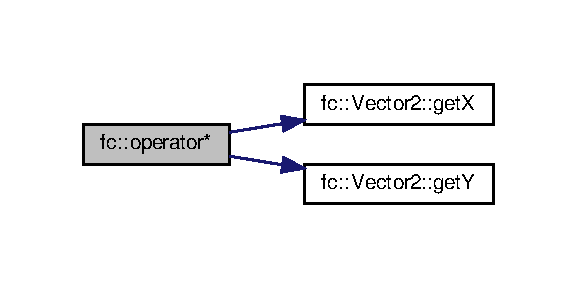
\includegraphics[width=277pt]{d2/db4/namespacefc_a29cd1b829e901810afd80ee5f75cdcc2_cgraph}
\end{center}
\end{figure}
\mbox{\Hypertarget{namespacefc_a54dd7df4c8a01e800426c7aefe3b349b}\label{namespacefc_a54dd7df4c8a01e800426c7aefe3b349b}} 
\index{fc@{fc}!operator+@{operator+}}
\index{operator+@{operator+}!fc@{fc}}
\subsubsection{\texorpdfstring{operator+()}{operator+()}}
{\footnotesize\ttfamily template$<$class eleT $>$ \\
\hyperlink{classfc_1_1Vector2}{Vector2}$<$eleT$>$ fc\+::operator+ (\begin{DoxyParamCaption}\item[{eleT}]{a,  }\item[{\hyperlink{classfc_1_1Vector2}{Vector2}$<$ eleT $>$}]{b }\end{DoxyParamCaption})}



Definition at line 422 of file Vector2.\+h.

Here is the call graph for this function\+:
\nopagebreak
\begin{figure}[H]
\begin{center}
\leavevmode
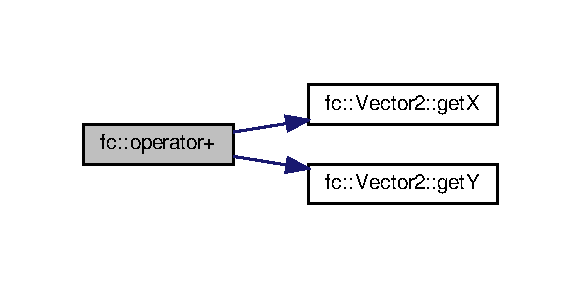
\includegraphics[width=279pt]{d2/db4/namespacefc_a54dd7df4c8a01e800426c7aefe3b349b_cgraph}
\end{center}
\end{figure}
\mbox{\Hypertarget{namespacefc_a851bc28427c29f20a4433485c0ae7afd}\label{namespacefc_a851bc28427c29f20a4433485c0ae7afd}} 
\index{fc@{fc}!operator-\/@{operator-\/}}
\index{operator-\/@{operator-\/}!fc@{fc}}
\subsubsection{\texorpdfstring{operator-\/()}{operator-()}}
{\footnotesize\ttfamily template$<$class eleT $>$ \\
\hyperlink{classfc_1_1Vector2}{Vector2}$<$eleT$>$ fc\+::operator-\/ (\begin{DoxyParamCaption}\item[{eleT}]{a,  }\item[{\hyperlink{classfc_1_1Vector2}{Vector2}$<$ eleT $>$}]{b }\end{DoxyParamCaption})}



Definition at line 429 of file Vector2.\+h.

Here is the call graph for this function\+:
\nopagebreak
\begin{figure}[H]
\begin{center}
\leavevmode
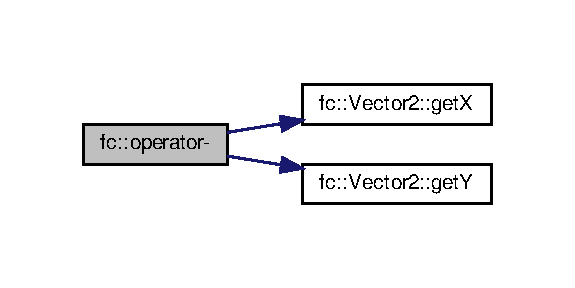
\includegraphics[width=276pt]{d2/db4/namespacefc_a851bc28427c29f20a4433485c0ae7afd_cgraph}
\end{center}
\end{figure}
\mbox{\Hypertarget{namespacefc_a639753beb1103357bce89497028a1443}\label{namespacefc_a639753beb1103357bce89497028a1443}} 
\index{fc@{fc}!operator/@{operator/}}
\index{operator/@{operator/}!fc@{fc}}
\subsubsection{\texorpdfstring{operator/()}{operator/()}}
{\footnotesize\ttfamily template$<$class eleT $>$ \\
\hyperlink{classfc_1_1Vector2}{Vector2}$<$eleT$>$ fc\+::operator/ (\begin{DoxyParamCaption}\item[{eleT}]{a,  }\item[{\hyperlink{classfc_1_1Vector2}{Vector2}$<$ eleT $>$}]{b }\end{DoxyParamCaption})}



Definition at line 443 of file Vector2.\+h.

Here is the call graph for this function\+:
\nopagebreak
\begin{figure}[H]
\begin{center}
\leavevmode
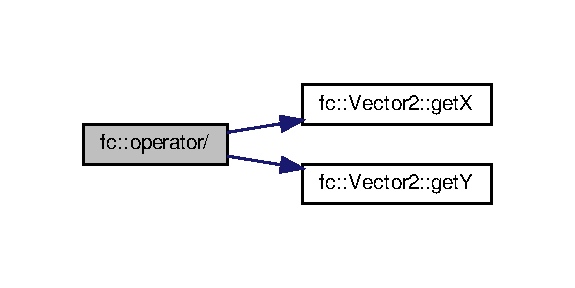
\includegraphics[width=276pt]{d2/db4/namespacefc_a639753beb1103357bce89497028a1443_cgraph}
\end{center}
\end{figure}
\mbox{\Hypertarget{namespacefc_a032cdf3cc33e52b02c4b66f65fc532b2}\label{namespacefc_a032cdf3cc33e52b02c4b66f65fc532b2}} 
\index{fc@{fc}!operator$<$$<$@{operator$<$$<$}}
\index{operator$<$$<$@{operator$<$$<$}!fc@{fc}}
\subsubsection{\texorpdfstring{operator$<$$<$()}{operator<<()}\hspace{0.1cm}{\footnotesize\ttfamily [1/2]}}
{\footnotesize\ttfamily template$<$class T $>$ \\
std\+::ostream\& fc\+::operator$<$$<$ (\begin{DoxyParamCaption}\item[{std\+::ostream \&}]{os,  }\item[{const \hyperlink{classfc_1_1Cuboid}{Cuboid}$<$ T $>$ \&}]{rhs }\end{DoxyParamCaption})}



Definition at line 93 of file Cuboid.\+h.

\mbox{\Hypertarget{namespacefc_a17fbd695ac7dd053e973c0e60f93061c}\label{namespacefc_a17fbd695ac7dd053e973c0e60f93061c}} 
\index{fc@{fc}!operator$<$$<$@{operator$<$$<$}}
\index{operator$<$$<$@{operator$<$$<$}!fc@{fc}}
\subsubsection{\texorpdfstring{operator$<$$<$()}{operator<<()}\hspace{0.1cm}{\footnotesize\ttfamily [2/2]}}
{\footnotesize\ttfamily template$<$class eleT $>$ \\
std\+::ostream\& fc\+::operator$<$$<$ (\begin{DoxyParamCaption}\item[{std\+::ostream \&}]{os,  }\item[{const \hyperlink{classfc_1_1Vector2}{Vector2}$<$ eleT $>$ \&}]{rhs }\end{DoxyParamCaption})}



Definition at line 181 of file Vector2.\+h.


\hypertarget{namespacefi}{}\section{fi Namespace Reference}
\label{namespacefi}\index{fi@{fi}}


\hyperlink{classfi_1_1FastImage}{Fast\+Image} namespace.  


\subsection*{Classes}
\begin{DoxyCompactItemize}
\item 
class \hyperlink{classfi_1_1ATileLoader}{A\+Tile\+Loader}
\begin{DoxyCompactList}\small\item\em Tile Loader interface. \end{DoxyCompactList}\item 
class \hyperlink{classfi_1_1CachedTile}{Cached\+Tile}
\begin{DoxyCompactList}\small\item\em Tile Cached from the file. \end{DoxyCompactList}\item 
class \hyperlink{classfi_1_1DistributePyramidRule}{Distribute\+Pyramid\+Rule}
\begin{DoxyCompactList}\small\item\em Distribute Pyramid Rule used by the execution pipeline. \end{DoxyCompactList}\item 
class \hyperlink{classfi_1_1FastImage}{Fast\+Image}
\begin{DoxyCompactList}\small\item\em Main api object to access the targeted image. \end{DoxyCompactList}\item 
class \hyperlink{classfi_1_1FastImageException}{Fast\+Image\+Exception}
\begin{DoxyCompactList}\small\item\em Exception specialized for Fast Image. \end{DoxyCompactList}\item 
class \hyperlink{classfi_1_1FigCache}{Fig\+Cache}
\begin{DoxyCompactList}\small\item\em Fast Image cache. \end{DoxyCompactList}\item 
class \hyperlink{classfi_1_1GrayscaleTiffTileLoader}{Grayscale\+Tiff\+Tile\+Loader}
\begin{DoxyCompactList}\small\item\em Tile loader specialized in grayscale tiff file. Use libtiff library. \end{DoxyCompactList}\item 
class \hyperlink{classfi_1_1HTGSTileRequestData}{H\+T\+G\+S\+Tile\+Request\+Data}
\begin{DoxyCompactList}\small\item\em Data representing a tile request. \end{DoxyCompactList}\item 
class \hyperlink{classfi_1_1HTGSViewRequestData}{H\+T\+G\+S\+View\+Request\+Data}
\begin{DoxyCompactList}\small\item\em Data representing a view request. \end{DoxyCompactList}\item 
class \hyperlink{classfi_1_1ReleaseCountRule}{Release\+Count\+Rule}
\begin{DoxyCompactList}\small\item\em Memory management release rule based on a count that is decremented after each use, and released when the count reaches 0. \end{DoxyCompactList}\item 
class \hyperlink{classfi_1_1Traversal}{Traversal}
\begin{DoxyCompactList}\small\item\em \hyperlink{classfi_1_1Traversal}{Traversal} object used to generate a vector of pair of coordinates. \end{DoxyCompactList}\item 
class \hyperlink{classfi_1_1VariableMemoryManager}{Variable\+Memory\+Manager}
\begin{DoxyCompactList}\small\item\em Variable Memory manager used to manage the memory for each pyramid level. \end{DoxyCompactList}\item 
class \hyperlink{classfi_1_1View}{View}
\begin{DoxyCompactList}\small\item\em \hyperlink{classfi_1_1View}{View} used by \hyperlink{classfi_1_1FastImage}{Fast\+Image} to represent image\textquotesingle{}s region. \end{DoxyCompactList}\item 
class \hyperlink{classfi_1_1ViewAllocator}{View\+Allocator}
\begin{DoxyCompactList}\small\item\em \hyperlink{classfi_1_1View}{View} Allocator allocates a \hyperlink{classfi_1_1FastImage}{Fast\+Image} view that is used by the H\+T\+GS memory manager. \end{DoxyCompactList}\item 
class \hyperlink{classfi_1_1ViewCounter}{View\+Counter}
\begin{DoxyCompactList}\small\item\em \hyperlink{classfi_1_1View}{View} Counter, graph\textquotesingle{}s last task, finalise the view. \end{DoxyCompactList}\item 
class \hyperlink{classfi_1_1ViewLoader}{View\+Loader}
\begin{DoxyCompactList}\small\item\em \hyperlink{classfi_1_1View}{View} loader task. Take a \hyperlink{classfi_1_1HTGSViewRequestData}{H\+T\+G\+S\+View\+Request\+Data} and produce a \hyperlink{classfi_1_1HTGSTileRequestData}{H\+T\+G\+S\+Tile\+Request\+Data}. \end{DoxyCompactList}\end{DoxyCompactItemize}
\subsection*{Enumerations}
\begin{DoxyCompactItemize}
\item 
enum \hyperlink{namespacefi_a6808b618c85d179a330ca388162215bd}{Filling\+Type} \{ \hyperlink{namespacefi_a6808b618c85d179a330ca388162215bdae8225b11842409df543692aebed34fd1}{Filling\+Type\+::\+F\+I\+LL}
 \}\begin{DoxyCompactList}\small\item\em Filling Strategy for ghost regions. \end{DoxyCompactList}
\item 
enum \hyperlink{namespacefi_a7ba5ce68668e7f273b22e5f56ca6dfcb}{Traversal\+Type} \{ \newline
\hyperlink{namespacefi_a7ba5ce68668e7f273b22e5f56ca6dfcba33e8270128b994b16da5c9e367bb94cf}{Traversal\+Type\+::\+N\+A\+I\+VE}, 
\hyperlink{namespacefi_a7ba5ce68668e7f273b22e5f56ca6dfcba6a30da74d0b15b45ec14072c93b6645d}{Traversal\+Type\+::\+S\+N\+A\+KE}, 
\hyperlink{namespacefi_a7ba5ce68668e7f273b22e5f56ca6dfcbad3fbf8a4dbb33b1e296fcaa32703b66d}{Traversal\+Type\+::\+D\+I\+A\+G\+O\+N\+AL}, 
\hyperlink{namespacefi_a7ba5ce68668e7f273b22e5f56ca6dfcba778dce36564f152ab7c452d6e5b773e9}{Traversal\+Type\+::\+H\+I\+L\+B\+E\+RT}, 
\newline
\hyperlink{namespacefi_a7ba5ce68668e7f273b22e5f56ca6dfcba550c81f476de2243dc93872a898ea918}{Traversal\+Type\+::\+S\+P\+I\+R\+AL}
 \}\begin{DoxyCompactList}\small\item\em Different traversal name. \end{DoxyCompactList}
\item 
enum \hyperlink{namespacefi_ac2e0fa52c14712db1a6e70da35ae8352}{Direction} \{ \hyperlink{namespacefi_ac2e0fa52c14712db1a6e70da35ae8352a2bf8f791695c70efa9c14e6f1c326403}{Direction\+::\+N\+O\+R\+TH}, 
\hyperlink{namespacefi_ac2e0fa52c14712db1a6e70da35ae8352a96e44fa82e5a5263fb92337be422d3eb}{Direction\+::\+S\+O\+U\+TH}, 
\hyperlink{namespacefi_ac2e0fa52c14712db1a6e70da35ae8352a45ac78bf3d4882ac520f4e7fb08d55c5}{Direction\+::\+E\+A\+ST}, 
\hyperlink{namespacefi_ac2e0fa52c14712db1a6e70da35ae8352a83c9f5692281bf59471b13dfddb3af91}{Direction\+::\+W\+E\+ST}
 \}\begin{DoxyCompactList}\small\item\em Different direction. \end{DoxyCompactList}
\end{DoxyCompactItemize}
\subsection*{Variables}
\begin{DoxyCompactItemize}
\item 
const int \hyperlink{namespacefi_afe2f57440da92fd8c3eebda3a33e7556}{M\+A\+J\+O\+R\+\_\+\+V\+E\+R\+S\+I\+ON} = 1
\item 
const int \hyperlink{namespacefi_a879229879c7f2a74c9a8b26495ab64ae}{M\+I\+N\+O\+R\+\_\+\+V\+E\+R\+S\+I\+ON} = 0
\item 
const int \hyperlink{namespacefi_aaa7396b6cc73524dbd906ce5af6317fc}{P\+A\+T\+C\+H\+\_\+\+V\+E\+R\+S\+I\+ON} = 8
\item 
const std\+::string \hyperlink{namespacefi_afaee9ec38f2807bff312e7ea8ec993ce}{F\+U\+L\+L\+\_\+\+V\+E\+R\+S\+I\+ON} = \char`\"{}1.\+0.\+8\char`\"{}
\end{DoxyCompactItemize}


\subsection{Detailed Description}
\hyperlink{classfi_1_1FastImage}{Fast\+Image} namespace. 

\subsection{Enumeration Type Documentation}
\mbox{\Hypertarget{namespacefi_ac2e0fa52c14712db1a6e70da35ae8352}\label{namespacefi_ac2e0fa52c14712db1a6e70da35ae8352}} 
\index{fi@{fi}!Direction@{Direction}}
\index{Direction@{Direction}!fi@{fi}}
\subsubsection{\texorpdfstring{Direction}{Direction}}
{\footnotesize\ttfamily enum \hyperlink{namespacefi_ac2e0fa52c14712db1a6e70da35ae8352}{fi\+::\+Direction}\hspace{0.3cm}{\ttfamily [strong]}}



Different direction. 

\begin{DoxyEnumFields}{Enumerator}
\raisebox{\heightof{T}}[0pt][0pt]{\index{N\+O\+R\+TH@{N\+O\+R\+TH}!fi@{fi}}\index{fi@{fi}!N\+O\+R\+TH@{N\+O\+R\+TH}}}\mbox{\Hypertarget{namespacefi_ac2e0fa52c14712db1a6e70da35ae8352a2bf8f791695c70efa9c14e6f1c326403}\label{namespacefi_ac2e0fa52c14712db1a6e70da35ae8352a2bf8f791695c70efa9c14e6f1c326403}} 
N\+O\+R\+TH&\\
\hline

\raisebox{\heightof{T}}[0pt][0pt]{\index{S\+O\+U\+TH@{S\+O\+U\+TH}!fi@{fi}}\index{fi@{fi}!S\+O\+U\+TH@{S\+O\+U\+TH}}}\mbox{\Hypertarget{namespacefi_ac2e0fa52c14712db1a6e70da35ae8352a96e44fa82e5a5263fb92337be422d3eb}\label{namespacefi_ac2e0fa52c14712db1a6e70da35ae8352a96e44fa82e5a5263fb92337be422d3eb}} 
S\+O\+U\+TH&\\
\hline

\raisebox{\heightof{T}}[0pt][0pt]{\index{E\+A\+ST@{E\+A\+ST}!fi@{fi}}\index{fi@{fi}!E\+A\+ST@{E\+A\+ST}}}\mbox{\Hypertarget{namespacefi_ac2e0fa52c14712db1a6e70da35ae8352a45ac78bf3d4882ac520f4e7fb08d55c5}\label{namespacefi_ac2e0fa52c14712db1a6e70da35ae8352a45ac78bf3d4882ac520f4e7fb08d55c5}} 
E\+A\+ST&\\
\hline

\raisebox{\heightof{T}}[0pt][0pt]{\index{W\+E\+ST@{W\+E\+ST}!fi@{fi}}\index{fi@{fi}!W\+E\+ST@{W\+E\+ST}}}\mbox{\Hypertarget{namespacefi_ac2e0fa52c14712db1a6e70da35ae8352a83c9f5692281bf59471b13dfddb3af91}\label{namespacefi_ac2e0fa52c14712db1a6e70da35ae8352a83c9f5692281bf59471b13dfddb3af91}} 
W\+E\+ST&\\
\hline

\end{DoxyEnumFields}


Definition at line 55 of file Data\+Type.\+h.

\mbox{\Hypertarget{namespacefi_a6808b618c85d179a330ca388162215bd}\label{namespacefi_a6808b618c85d179a330ca388162215bd}} 
\index{fi@{fi}!Filling\+Type@{Filling\+Type}}
\index{Filling\+Type@{Filling\+Type}!fi@{fi}}
\subsubsection{\texorpdfstring{Filling\+Type}{FillingType}}
{\footnotesize\ttfamily enum \hyperlink{namespacefi_a6808b618c85d179a330ca388162215bd}{fi\+::\+Filling\+Type}\hspace{0.3cm}{\ttfamily [strong]}}



Filling Strategy for ghost regions. 

\begin{DoxyEnumFields}{Enumerator}
\raisebox{\heightof{T}}[0pt][0pt]{\index{F\+I\+LL@{F\+I\+LL}!fi@{fi}}\index{fi@{fi}!F\+I\+LL@{F\+I\+LL}}}\mbox{\Hypertarget{namespacefi_a6808b618c85d179a330ca388162215bdae8225b11842409df543692aebed34fd1}\label{namespacefi_a6808b618c85d179a330ca388162215bdae8225b11842409df543692aebed34fd1}} 
F\+I\+LL&\\
\hline

\end{DoxyEnumFields}


Definition at line 41 of file Data\+Type.\+h.

\mbox{\Hypertarget{namespacefi_a7ba5ce68668e7f273b22e5f56ca6dfcb}\label{namespacefi_a7ba5ce68668e7f273b22e5f56ca6dfcb}} 
\index{fi@{fi}!Traversal\+Type@{Traversal\+Type}}
\index{Traversal\+Type@{Traversal\+Type}!fi@{fi}}
\subsubsection{\texorpdfstring{Traversal\+Type}{TraversalType}}
{\footnotesize\ttfamily enum \hyperlink{namespacefi_a7ba5ce68668e7f273b22e5f56ca6dfcb}{fi\+::\+Traversal\+Type}\hspace{0.3cm}{\ttfamily [strong]}}



Different traversal name. 

\begin{DoxyEnumFields}{Enumerator}
\raisebox{\heightof{T}}[0pt][0pt]{\index{N\+A\+I\+VE@{N\+A\+I\+VE}!fi@{fi}}\index{fi@{fi}!N\+A\+I\+VE@{N\+A\+I\+VE}}}\mbox{\Hypertarget{namespacefi_a7ba5ce68668e7f273b22e5f56ca6dfcba33e8270128b994b16da5c9e367bb94cf}\label{namespacefi_a7ba5ce68668e7f273b22e5f56ca6dfcba33e8270128b994b16da5c9e367bb94cf}} 
N\+A\+I\+VE&\\
\hline

\raisebox{\heightof{T}}[0pt][0pt]{\index{S\+N\+A\+KE@{S\+N\+A\+KE}!fi@{fi}}\index{fi@{fi}!S\+N\+A\+KE@{S\+N\+A\+KE}}}\mbox{\Hypertarget{namespacefi_a7ba5ce68668e7f273b22e5f56ca6dfcba6a30da74d0b15b45ec14072c93b6645d}\label{namespacefi_a7ba5ce68668e7f273b22e5f56ca6dfcba6a30da74d0b15b45ec14072c93b6645d}} 
S\+N\+A\+KE&\\
\hline

\raisebox{\heightof{T}}[0pt][0pt]{\index{D\+I\+A\+G\+O\+N\+AL@{D\+I\+A\+G\+O\+N\+AL}!fi@{fi}}\index{fi@{fi}!D\+I\+A\+G\+O\+N\+AL@{D\+I\+A\+G\+O\+N\+AL}}}\mbox{\Hypertarget{namespacefi_a7ba5ce68668e7f273b22e5f56ca6dfcbad3fbf8a4dbb33b1e296fcaa32703b66d}\label{namespacefi_a7ba5ce68668e7f273b22e5f56ca6dfcbad3fbf8a4dbb33b1e296fcaa32703b66d}} 
D\+I\+A\+G\+O\+N\+AL&\\
\hline

\raisebox{\heightof{T}}[0pt][0pt]{\index{H\+I\+L\+B\+E\+RT@{H\+I\+L\+B\+E\+RT}!fi@{fi}}\index{fi@{fi}!H\+I\+L\+B\+E\+RT@{H\+I\+L\+B\+E\+RT}}}\mbox{\Hypertarget{namespacefi_a7ba5ce68668e7f273b22e5f56ca6dfcba778dce36564f152ab7c452d6e5b773e9}\label{namespacefi_a7ba5ce68668e7f273b22e5f56ca6dfcba778dce36564f152ab7c452d6e5b773e9}} 
H\+I\+L\+B\+E\+RT&\\
\hline

\raisebox{\heightof{T}}[0pt][0pt]{\index{S\+P\+I\+R\+AL@{S\+P\+I\+R\+AL}!fi@{fi}}\index{fi@{fi}!S\+P\+I\+R\+AL@{S\+P\+I\+R\+AL}}}\mbox{\Hypertarget{namespacefi_a7ba5ce68668e7f273b22e5f56ca6dfcba550c81f476de2243dc93872a898ea918}\label{namespacefi_a7ba5ce68668e7f273b22e5f56ca6dfcba550c81f476de2243dc93872a898ea918}} 
S\+P\+I\+R\+AL&\\
\hline

\end{DoxyEnumFields}


Definition at line 46 of file Data\+Type.\+h.



\subsection{Variable Documentation}
\mbox{\Hypertarget{namespacefi_afaee9ec38f2807bff312e7ea8ec993ce}\label{namespacefi_afaee9ec38f2807bff312e7ea8ec993ce}} 
\index{fi@{fi}!F\+U\+L\+L\+\_\+\+V\+E\+R\+S\+I\+ON@{F\+U\+L\+L\+\_\+\+V\+E\+R\+S\+I\+ON}}
\index{F\+U\+L\+L\+\_\+\+V\+E\+R\+S\+I\+ON@{F\+U\+L\+L\+\_\+\+V\+E\+R\+S\+I\+ON}!fi@{fi}}
\subsubsection{\texorpdfstring{F\+U\+L\+L\+\_\+\+V\+E\+R\+S\+I\+ON}{FULL\_VERSION}}
{\footnotesize\ttfamily const std\+::string fi\+::\+F\+U\+L\+L\+\_\+\+V\+E\+R\+S\+I\+ON = \char`\"{}1.\+0.\+8\char`\"{}}



Definition at line 15 of file Version.\+h.

\mbox{\Hypertarget{namespacefi_afe2f57440da92fd8c3eebda3a33e7556}\label{namespacefi_afe2f57440da92fd8c3eebda3a33e7556}} 
\index{fi@{fi}!M\+A\+J\+O\+R\+\_\+\+V\+E\+R\+S\+I\+ON@{M\+A\+J\+O\+R\+\_\+\+V\+E\+R\+S\+I\+ON}}
\index{M\+A\+J\+O\+R\+\_\+\+V\+E\+R\+S\+I\+ON@{M\+A\+J\+O\+R\+\_\+\+V\+E\+R\+S\+I\+ON}!fi@{fi}}
\subsubsection{\texorpdfstring{M\+A\+J\+O\+R\+\_\+\+V\+E\+R\+S\+I\+ON}{MAJOR\_VERSION}}
{\footnotesize\ttfamily const int fi\+::\+M\+A\+J\+O\+R\+\_\+\+V\+E\+R\+S\+I\+ON = 1}



Definition at line 12 of file Version.\+h.

\mbox{\Hypertarget{namespacefi_a879229879c7f2a74c9a8b26495ab64ae}\label{namespacefi_a879229879c7f2a74c9a8b26495ab64ae}} 
\index{fi@{fi}!M\+I\+N\+O\+R\+\_\+\+V\+E\+R\+S\+I\+ON@{M\+I\+N\+O\+R\+\_\+\+V\+E\+R\+S\+I\+ON}}
\index{M\+I\+N\+O\+R\+\_\+\+V\+E\+R\+S\+I\+ON@{M\+I\+N\+O\+R\+\_\+\+V\+E\+R\+S\+I\+ON}!fi@{fi}}
\subsubsection{\texorpdfstring{M\+I\+N\+O\+R\+\_\+\+V\+E\+R\+S\+I\+ON}{MINOR\_VERSION}}
{\footnotesize\ttfamily const int fi\+::\+M\+I\+N\+O\+R\+\_\+\+V\+E\+R\+S\+I\+ON = 0}



Definition at line 13 of file Version.\+h.

\mbox{\Hypertarget{namespacefi_aaa7396b6cc73524dbd906ce5af6317fc}\label{namespacefi_aaa7396b6cc73524dbd906ce5af6317fc}} 
\index{fi@{fi}!P\+A\+T\+C\+H\+\_\+\+V\+E\+R\+S\+I\+ON@{P\+A\+T\+C\+H\+\_\+\+V\+E\+R\+S\+I\+ON}}
\index{P\+A\+T\+C\+H\+\_\+\+V\+E\+R\+S\+I\+ON@{P\+A\+T\+C\+H\+\_\+\+V\+E\+R\+S\+I\+ON}!fi@{fi}}
\subsubsection{\texorpdfstring{P\+A\+T\+C\+H\+\_\+\+V\+E\+R\+S\+I\+ON}{PATCH\_VERSION}}
{\footnotesize\ttfamily const int fi\+::\+P\+A\+T\+C\+H\+\_\+\+V\+E\+R\+S\+I\+ON = 8}



Definition at line 14 of file Version.\+h.


\chapter{Class Documentation}
\hypertarget{structfc_1_1AABBTree_1_1AABBNode}{}\section{fc\+:\+:A\+A\+B\+B\+Tree$<$ ObjectT $>$\+:\+:A\+A\+B\+B\+Node Struct Reference}
\label{structfc_1_1AABBTree_1_1AABBNode}\index{fc\+::\+A\+A\+B\+B\+Tree$<$ Object\+T $>$\+::\+A\+A\+B\+B\+Node@{fc\+::\+A\+A\+B\+B\+Tree$<$ Object\+T $>$\+::\+A\+A\+B\+B\+Node}}


Collaboration diagram for fc\+:\+:A\+A\+B\+B\+Tree$<$ ObjectT $>$\+:\+:A\+A\+B\+B\+Node\+:
\nopagebreak
\begin{figure}[H]
\begin{center}
\leavevmode
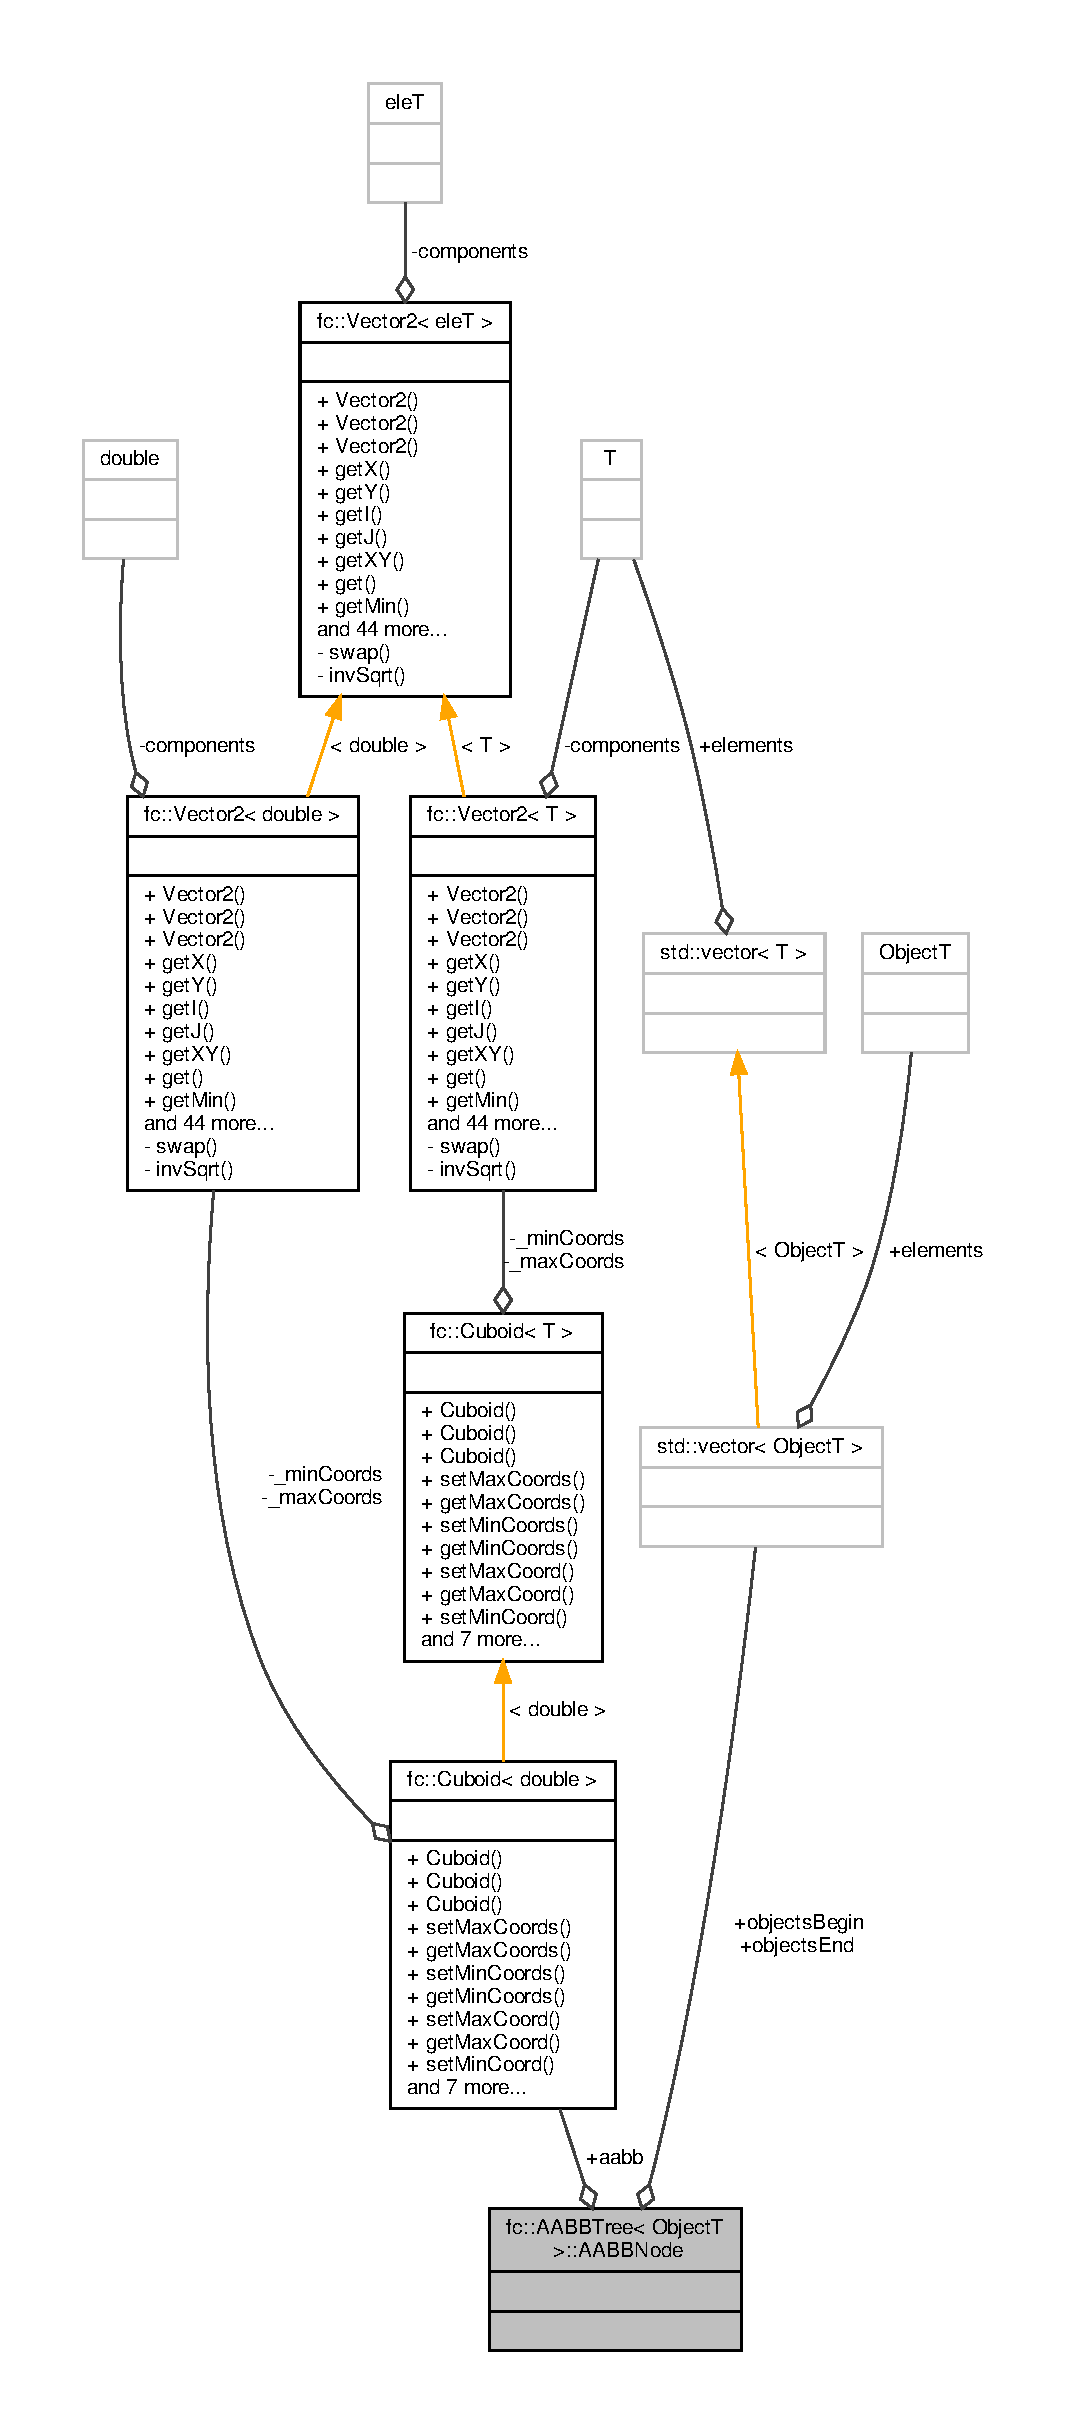
\includegraphics[height=550pt]{d6/d9a/structfc_1_1AABBTree_1_1AABBNode__coll__graph}
\end{center}
\end{figure}
\subsection*{Public Attributes}
\begin{DoxyCompactItemize}
\item 
\hyperlink{classfc_1_1Cuboid}{Cuboid}$<$ double $>$ \hyperlink{structfc_1_1AABBTree_1_1AABBNode_ac4016fa848e48a4270fc1f4ceb0cfec8}{aabb}
\item 
\hyperlink{classfc_1_1AABBTree_a3333c421c1fa34841043bd8545de8ea8}{objects\+\_\+size\+\_\+type} \hyperlink{structfc_1_1AABBTree_1_1AABBNode_a705257db430984c00801167f5a561970}{objects\+Begin}
\item 
\hyperlink{classfc_1_1AABBTree_a3333c421c1fa34841043bd8545de8ea8}{objects\+\_\+size\+\_\+type} \hyperlink{structfc_1_1AABBTree_1_1AABBNode_a4033832124c05f502e35f7ffdb5abc56}{objects\+End}
\end{DoxyCompactItemize}


\subsection{Detailed Description}
\subsubsection*{template$<$class ObjectT$>$\newline
struct fc\+::\+A\+A\+B\+B\+Tree$<$ Object\+T $>$\+::\+A\+A\+B\+B\+Node}



Definition at line 66 of file A\+A\+B\+B\+Tree.\+h.



\subsection{Member Data Documentation}
\mbox{\Hypertarget{structfc_1_1AABBTree_1_1AABBNode_ac4016fa848e48a4270fc1f4ceb0cfec8}\label{structfc_1_1AABBTree_1_1AABBNode_ac4016fa848e48a4270fc1f4ceb0cfec8}} 
\index{fc\+::\+A\+A\+B\+B\+Tree\+::\+A\+A\+B\+B\+Node@{fc\+::\+A\+A\+B\+B\+Tree\+::\+A\+A\+B\+B\+Node}!aabb@{aabb}}
\index{aabb@{aabb}!fc\+::\+A\+A\+B\+B\+Tree\+::\+A\+A\+B\+B\+Node@{fc\+::\+A\+A\+B\+B\+Tree\+::\+A\+A\+B\+B\+Node}}
\subsubsection{\texorpdfstring{aabb}{aabb}}
{\footnotesize\ttfamily template$<$class ObjectT$>$ \\
\hyperlink{classfc_1_1Cuboid}{Cuboid}$<$double$>$ \hyperlink{classfc_1_1AABBTree}{fc\+::\+A\+A\+B\+B\+Tree}$<$ ObjectT $>$\+::A\+A\+B\+B\+Node\+::aabb}



Definition at line 67 of file A\+A\+B\+B\+Tree.\+h.

\mbox{\Hypertarget{structfc_1_1AABBTree_1_1AABBNode_a705257db430984c00801167f5a561970}\label{structfc_1_1AABBTree_1_1AABBNode_a705257db430984c00801167f5a561970}} 
\index{fc\+::\+A\+A\+B\+B\+Tree\+::\+A\+A\+B\+B\+Node@{fc\+::\+A\+A\+B\+B\+Tree\+::\+A\+A\+B\+B\+Node}!objects\+Begin@{objects\+Begin}}
\index{objects\+Begin@{objects\+Begin}!fc\+::\+A\+A\+B\+B\+Tree\+::\+A\+A\+B\+B\+Node@{fc\+::\+A\+A\+B\+B\+Tree\+::\+A\+A\+B\+B\+Node}}
\subsubsection{\texorpdfstring{objects\+Begin}{objectsBegin}}
{\footnotesize\ttfamily template$<$class ObjectT$>$ \\
\hyperlink{classfc_1_1AABBTree_a3333c421c1fa34841043bd8545de8ea8}{objects\+\_\+size\+\_\+type} \hyperlink{classfc_1_1AABBTree}{fc\+::\+A\+A\+B\+B\+Tree}$<$ ObjectT $>$\+::A\+A\+B\+B\+Node\+::objects\+Begin}



Definition at line 69 of file A\+A\+B\+B\+Tree.\+h.

\mbox{\Hypertarget{structfc_1_1AABBTree_1_1AABBNode_a4033832124c05f502e35f7ffdb5abc56}\label{structfc_1_1AABBTree_1_1AABBNode_a4033832124c05f502e35f7ffdb5abc56}} 
\index{fc\+::\+A\+A\+B\+B\+Tree\+::\+A\+A\+B\+B\+Node@{fc\+::\+A\+A\+B\+B\+Tree\+::\+A\+A\+B\+B\+Node}!objects\+End@{objects\+End}}
\index{objects\+End@{objects\+End}!fc\+::\+A\+A\+B\+B\+Tree\+::\+A\+A\+B\+B\+Node@{fc\+::\+A\+A\+B\+B\+Tree\+::\+A\+A\+B\+B\+Node}}
\subsubsection{\texorpdfstring{objects\+End}{objectsEnd}}
{\footnotesize\ttfamily template$<$class ObjectT$>$ \\
\hyperlink{classfc_1_1AABBTree_a3333c421c1fa34841043bd8545de8ea8}{objects\+\_\+size\+\_\+type} \hyperlink{classfc_1_1AABBTree}{fc\+::\+A\+A\+B\+B\+Tree}$<$ ObjectT $>$\+::A\+A\+B\+B\+Node\+::objects\+End}



Definition at line 70 of file A\+A\+B\+B\+Tree.\+h.



The documentation for this struct was generated from the following file\+:\begin{DoxyCompactItemize}
\item 
/home/anb22/\+Documents/\+Fast-\/\+Image/\+Fast\+Image/src/\+Fast\+Image/\+Feature\+Collection/tools/\hyperlink{AABBTree_8h}{A\+A\+B\+B\+Tree.\+h}\end{DoxyCompactItemize}

\hypertarget{classfc_1_1AABBTree}{}\section{fc\+:\+:A\+A\+B\+B\+Tree$<$ ObjectT $>$ Class Template Reference}
\label{classfc_1_1AABBTree}\index{fc\+::\+A\+A\+B\+B\+Tree$<$ Object\+T $>$@{fc\+::\+A\+A\+B\+B\+Tree$<$ Object\+T $>$}}


{\ttfamily \#include $<$A\+A\+B\+B\+Tree.\+h$>$}



Inheritance diagram for fc\+:\+:A\+A\+B\+B\+Tree$<$ ObjectT $>$\+:
\nopagebreak
\begin{figure}[H]
\begin{center}
\leavevmode
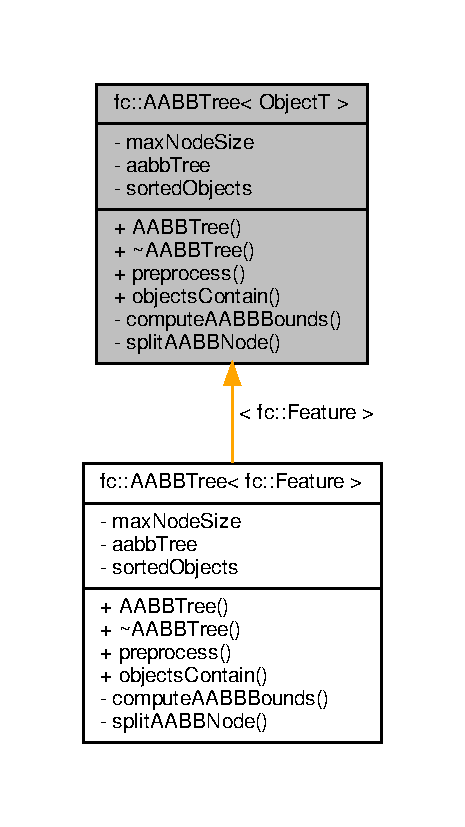
\includegraphics[width=223pt]{dd/d48/classfc_1_1AABBTree__inherit__graph}
\end{center}
\end{figure}


Collaboration diagram for fc\+:\+:A\+A\+B\+B\+Tree$<$ ObjectT $>$\+:
\nopagebreak
\begin{figure}[H]
\begin{center}
\leavevmode
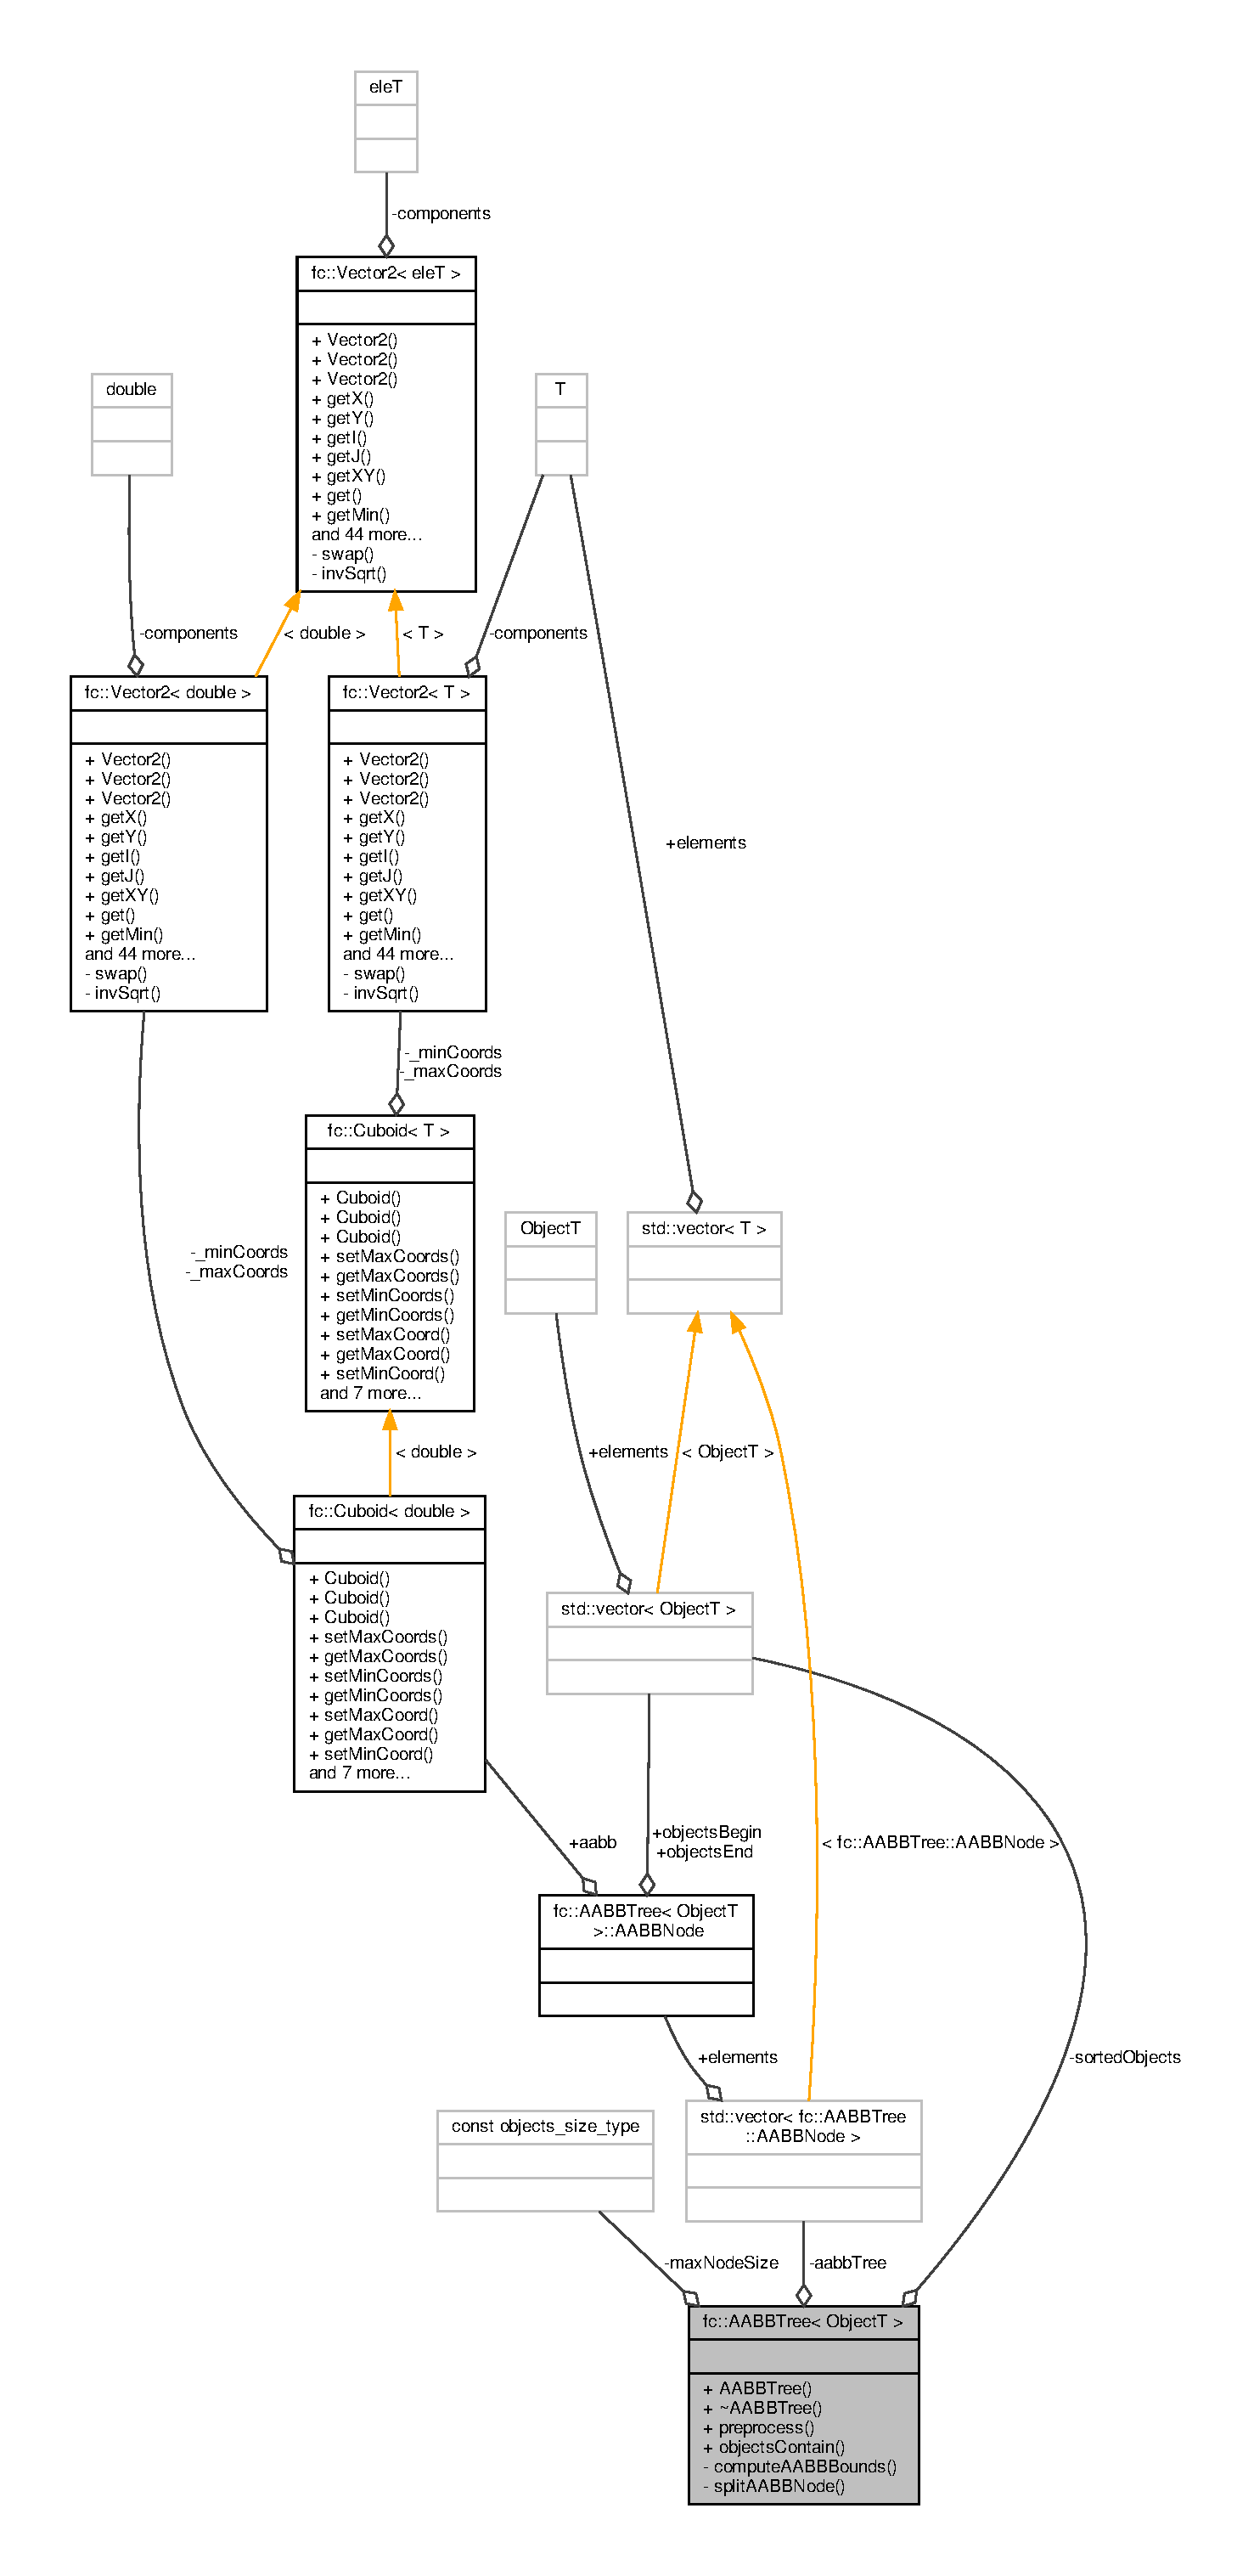
\includegraphics[height=550pt]{d0/dea/classfc_1_1AABBTree__coll__graph}
\end{center}
\end{figure}
\subsection*{Classes}
\begin{DoxyCompactItemize}
\item 
struct \hyperlink{structfc_1_1AABBTree_1_1AABBNode}{A\+A\+B\+B\+Node}
\end{DoxyCompactItemize}
\subsection*{Public Member Functions}
\begin{DoxyCompactItemize}
\item 
\hyperlink{classfc_1_1AABBTree_a4d8525582030f9cc79b68ed97271c000}{A\+A\+B\+B\+Tree} (\hyperlink{classfc_1_1AABBTree_a3333c421c1fa34841043bd8545de8ea8}{objects\+\_\+size\+\_\+type} \hyperlink{classfc_1_1AABBTree_a4116e801983d055e249fa6166fa47266}{max\+Node\+Size}=4)
\item 
\hyperlink{classfc_1_1AABBTree_a13dfddea7618153509ca07e14334cfe0}{$\sim$\+A\+A\+B\+B\+Tree} ()
\item 
void \hyperlink{classfc_1_1AABBTree_a481a24bdded9dfbebfcb298899126df3}{preprocess} (std\+::vector$<$ ObjectT $>$ $\ast$objects)
\item 
std\+::vector$<$ ObjectT $\ast$ $>$ \hyperlink{classfc_1_1AABBTree_aef6e5c039251417ae18f17cf9f30f638}{objects\+Contain} (\hyperlink{classfc_1_1Vector2}{Vector2}$<$ double $>$ const \&query\+Point) const
\end{DoxyCompactItemize}
\subsection*{Private Types}
\begin{DoxyCompactItemize}
\item 
using \hyperlink{classfc_1_1AABBTree_a3333c421c1fa34841043bd8545de8ea8}{objects\+\_\+size\+\_\+type} = typename std\+::vector$<$ ObjectT $>$\+::size\+\_\+type
\item 
using \hyperlink{classfc_1_1AABBTree_a18706db5b992d8875e08dc325abf3811}{aabb\+Tree\+\_\+size\+\_\+type} = typename std\+::vector$<$ \hyperlink{structfc_1_1AABBTree_1_1AABBNode}{A\+A\+B\+B\+Node} $>$\+::size\+\_\+type
\end{DoxyCompactItemize}
\subsection*{Private Member Functions}
\begin{DoxyCompactItemize}
\item 
void \hyperlink{classfc_1_1AABBTree_aac657a296e6a26e675a259c5d3fef53d}{compute\+A\+A\+B\+B\+Bounds} (\hyperlink{classfc_1_1AABBTree_a18706db5b992d8875e08dc325abf3811}{aabb\+Tree\+\_\+size\+\_\+type} node\+Index)
\item 
void \hyperlink{classfc_1_1AABBTree_a01f4466619083a8820f721cff76831dc}{split\+A\+A\+B\+B\+Node} (\hyperlink{classfc_1_1AABBTree_a18706db5b992d8875e08dc325abf3811}{aabb\+Tree\+\_\+size\+\_\+type} node\+Index, int split\+Dim)
\end{DoxyCompactItemize}
\subsection*{Private Attributes}
\begin{DoxyCompactItemize}
\item 
const \hyperlink{classfc_1_1AABBTree_a3333c421c1fa34841043bd8545de8ea8}{objects\+\_\+size\+\_\+type} \hyperlink{classfc_1_1AABBTree_a4116e801983d055e249fa6166fa47266}{max\+Node\+Size}
\item 
std\+::vector$<$ \hyperlink{structfc_1_1AABBTree_1_1AABBNode}{A\+A\+B\+B\+Node} $>$ \hyperlink{classfc_1_1AABBTree_a971132f54e3a462458362901fac9b37f}{aabb\+Tree}
\item 
std\+::vector$<$ ObjectT $>$ $\ast$ \hyperlink{classfc_1_1AABBTree_ad28d9de49d42c0dffae1f6c47be5b523}{sorted\+Objects}
\end{DoxyCompactItemize}


\subsection{Detailed Description}
\subsubsection*{template$<$class ObjectT$>$\newline
class fc\+::\+A\+A\+B\+B\+Tree$<$ Object\+T $>$}

Spatial data structure for nearest-\/object queries based on an Axis Aligned Bounding Box (A\+A\+BB) tree. The data structure can store any objects which themselves can be enclosed in an A\+A\+BB and which can compute their distance to a point. Specifically, the objects must provide the following functions\+:

double get\+Max\+Coord(int dim) double get\+Min\+Coord(int dim) double get\+Distance\+Sqr\+To(\+Vector2$<$double$>$ const \& point) bool contains(\+Vector2$<$double$>$ const \& point) 

Definition at line 63 of file A\+A\+B\+B\+Tree.\+h.



\subsection{Member Typedef Documentation}
\mbox{\Hypertarget{classfc_1_1AABBTree_a18706db5b992d8875e08dc325abf3811}\label{classfc_1_1AABBTree_a18706db5b992d8875e08dc325abf3811}} 
\index{fc\+::\+A\+A\+B\+B\+Tree@{fc\+::\+A\+A\+B\+B\+Tree}!aabb\+Tree\+\_\+size\+\_\+type@{aabb\+Tree\+\_\+size\+\_\+type}}
\index{aabb\+Tree\+\_\+size\+\_\+type@{aabb\+Tree\+\_\+size\+\_\+type}!fc\+::\+A\+A\+B\+B\+Tree@{fc\+::\+A\+A\+B\+B\+Tree}}
\subsubsection{\texorpdfstring{aabb\+Tree\+\_\+size\+\_\+type}{aabbTree\_size\_type}}
{\footnotesize\ttfamily template$<$class ObjectT$>$ \\
using \hyperlink{classfc_1_1AABBTree}{fc\+::\+A\+A\+B\+B\+Tree}$<$ ObjectT $>$\+::\hyperlink{classfc_1_1AABBTree_a18706db5b992d8875e08dc325abf3811}{aabb\+Tree\+\_\+size\+\_\+type} =  typename std\+::vector$<$\hyperlink{structfc_1_1AABBTree_1_1AABBNode}{A\+A\+B\+B\+Node}$>$\+::size\+\_\+type\hspace{0.3cm}{\ttfamily [private]}}



Definition at line 72 of file A\+A\+B\+B\+Tree.\+h.

\mbox{\Hypertarget{classfc_1_1AABBTree_a3333c421c1fa34841043bd8545de8ea8}\label{classfc_1_1AABBTree_a3333c421c1fa34841043bd8545de8ea8}} 
\index{fc\+::\+A\+A\+B\+B\+Tree@{fc\+::\+A\+A\+B\+B\+Tree}!objects\+\_\+size\+\_\+type@{objects\+\_\+size\+\_\+type}}
\index{objects\+\_\+size\+\_\+type@{objects\+\_\+size\+\_\+type}!fc\+::\+A\+A\+B\+B\+Tree@{fc\+::\+A\+A\+B\+B\+Tree}}
\subsubsection{\texorpdfstring{objects\+\_\+size\+\_\+type}{objects\_size\_type}}
{\footnotesize\ttfamily template$<$class ObjectT$>$ \\
using \hyperlink{classfc_1_1AABBTree}{fc\+::\+A\+A\+B\+B\+Tree}$<$ ObjectT $>$\+::\hyperlink{classfc_1_1AABBTree_a3333c421c1fa34841043bd8545de8ea8}{objects\+\_\+size\+\_\+type} =  typename std\+::vector$<$ObjectT$>$\+::size\+\_\+type\hspace{0.3cm}{\ttfamily [private]}}



Definition at line 65 of file A\+A\+B\+B\+Tree.\+h.



\subsection{Constructor \& Destructor Documentation}
\mbox{\Hypertarget{classfc_1_1AABBTree_a4d8525582030f9cc79b68ed97271c000}\label{classfc_1_1AABBTree_a4d8525582030f9cc79b68ed97271c000}} 
\index{fc\+::\+A\+A\+B\+B\+Tree@{fc\+::\+A\+A\+B\+B\+Tree}!A\+A\+B\+B\+Tree@{A\+A\+B\+B\+Tree}}
\index{A\+A\+B\+B\+Tree@{A\+A\+B\+B\+Tree}!fc\+::\+A\+A\+B\+B\+Tree@{fc\+::\+A\+A\+B\+B\+Tree}}
\subsubsection{\texorpdfstring{A\+A\+B\+B\+Tree()}{AABBTree()}}
{\footnotesize\ttfamily template$<$class ObjectT $>$ \\
\hyperlink{classfc_1_1AABBTree}{fc\+::\+A\+A\+B\+B\+Tree}$<$ ObjectT $>$\+::\hyperlink{classfc_1_1AABBTree}{A\+A\+B\+B\+Tree} (\begin{DoxyParamCaption}\item[{\hyperlink{classfc_1_1AABBTree_a3333c421c1fa34841043bd8545de8ea8}{objects\+\_\+size\+\_\+type}}]{max\+Node\+Size = {\ttfamily 4} }\end{DoxyParamCaption})\hspace{0.3cm}{\ttfamily [explicit]}}

Constructs an empty spatial data structure. 

Definition at line 101 of file A\+A\+B\+B\+Tree.\+h.

\mbox{\Hypertarget{classfc_1_1AABBTree_a13dfddea7618153509ca07e14334cfe0}\label{classfc_1_1AABBTree_a13dfddea7618153509ca07e14334cfe0}} 
\index{fc\+::\+A\+A\+B\+B\+Tree@{fc\+::\+A\+A\+B\+B\+Tree}!````~A\+A\+B\+B\+Tree@{$\sim$\+A\+A\+B\+B\+Tree}}
\index{````~A\+A\+B\+B\+Tree@{$\sim$\+A\+A\+B\+B\+Tree}!fc\+::\+A\+A\+B\+B\+Tree@{fc\+::\+A\+A\+B\+B\+Tree}}
\subsubsection{\texorpdfstring{$\sim$\+A\+A\+B\+B\+Tree()}{~AABBTree()}}
{\footnotesize\ttfamily template$<$class ObjectT $>$ \\
\hyperlink{classfc_1_1AABBTree}{fc\+::\+A\+A\+B\+B\+Tree}$<$ ObjectT $>$\+::$\sim$\hyperlink{classfc_1_1AABBTree}{A\+A\+B\+B\+Tree} (\begin{DoxyParamCaption}{ }\end{DoxyParamCaption})\hspace{0.3cm}{\ttfamily [default]}}



\subsection{Member Function Documentation}
\mbox{\Hypertarget{classfc_1_1AABBTree_aac657a296e6a26e675a259c5d3fef53d}\label{classfc_1_1AABBTree_aac657a296e6a26e675a259c5d3fef53d}} 
\index{fc\+::\+A\+A\+B\+B\+Tree@{fc\+::\+A\+A\+B\+B\+Tree}!compute\+A\+A\+B\+B\+Bounds@{compute\+A\+A\+B\+B\+Bounds}}
\index{compute\+A\+A\+B\+B\+Bounds@{compute\+A\+A\+B\+B\+Bounds}!fc\+::\+A\+A\+B\+B\+Tree@{fc\+::\+A\+A\+B\+B\+Tree}}
\subsubsection{\texorpdfstring{compute\+A\+A\+B\+B\+Bounds()}{computeAABBBounds()}}
{\footnotesize\ttfamily template$<$class ObjectT $>$ \\
void \hyperlink{classfc_1_1AABBTree}{fc\+::\+A\+A\+B\+B\+Tree}$<$ ObjectT $>$\+::compute\+A\+A\+B\+B\+Bounds (\begin{DoxyParamCaption}\item[{\hyperlink{classfc_1_1AABBTree_a18706db5b992d8875e08dc325abf3811}{aabb\+Tree\+\_\+size\+\_\+type}}]{node\+Index }\end{DoxyParamCaption})\hspace{0.3cm}{\ttfamily [private]}}



Definition at line 178 of file A\+A\+B\+B\+Tree.\+h.

\mbox{\Hypertarget{classfc_1_1AABBTree_aef6e5c039251417ae18f17cf9f30f638}\label{classfc_1_1AABBTree_aef6e5c039251417ae18f17cf9f30f638}} 
\index{fc\+::\+A\+A\+B\+B\+Tree@{fc\+::\+A\+A\+B\+B\+Tree}!objects\+Contain@{objects\+Contain}}
\index{objects\+Contain@{objects\+Contain}!fc\+::\+A\+A\+B\+B\+Tree@{fc\+::\+A\+A\+B\+B\+Tree}}
\subsubsection{\texorpdfstring{objects\+Contain()}{objectsContain()}}
{\footnotesize\ttfamily template$<$class ObjectT $>$ \\
std\+::vector$<$ ObjectT $\ast$ $>$ \hyperlink{classfc_1_1AABBTree}{fc\+::\+A\+A\+B\+B\+Tree}$<$ ObjectT $>$\+::objects\+Contain (\begin{DoxyParamCaption}\item[{\hyperlink{classfc_1_1Vector2}{Vector2}$<$ double $>$ const \&}]{query\+Point }\end{DoxyParamCaption}) const}

Returns whether any object in the tree contains the given query point. 

Definition at line 268 of file A\+A\+B\+B\+Tree.\+h.

\mbox{\Hypertarget{classfc_1_1AABBTree_a481a24bdded9dfbebfcb298899126df3}\label{classfc_1_1AABBTree_a481a24bdded9dfbebfcb298899126df3}} 
\index{fc\+::\+A\+A\+B\+B\+Tree@{fc\+::\+A\+A\+B\+B\+Tree}!preprocess@{preprocess}}
\index{preprocess@{preprocess}!fc\+::\+A\+A\+B\+B\+Tree@{fc\+::\+A\+A\+B\+B\+Tree}}
\subsubsection{\texorpdfstring{preprocess()}{preprocess()}}
{\footnotesize\ttfamily template$<$class ObjectT$>$ \\
void \hyperlink{classfc_1_1AABBTree}{fc\+::\+A\+A\+B\+B\+Tree}$<$ ObjectT $>$\+::preprocess (\begin{DoxyParamCaption}\item[{std\+::vector$<$ ObjectT $>$ $\ast$}]{objects }\end{DoxyParamCaption})}

Inserts the given objects into the spatial data structure. The objects vector may be modified and must not be changed outside the class. 

Definition at line 117 of file A\+A\+B\+B\+Tree.\+h.

\mbox{\Hypertarget{classfc_1_1AABBTree_a01f4466619083a8820f721cff76831dc}\label{classfc_1_1AABBTree_a01f4466619083a8820f721cff76831dc}} 
\index{fc\+::\+A\+A\+B\+B\+Tree@{fc\+::\+A\+A\+B\+B\+Tree}!split\+A\+A\+B\+B\+Node@{split\+A\+A\+B\+B\+Node}}
\index{split\+A\+A\+B\+B\+Node@{split\+A\+A\+B\+B\+Node}!fc\+::\+A\+A\+B\+B\+Tree@{fc\+::\+A\+A\+B\+B\+Tree}}
\subsubsection{\texorpdfstring{split\+A\+A\+B\+B\+Node()}{splitAABBNode()}}
{\footnotesize\ttfamily template$<$class ObjectT $>$ \\
void \hyperlink{classfc_1_1AABBTree}{fc\+::\+A\+A\+B\+B\+Tree}$<$ ObjectT $>$\+::split\+A\+A\+B\+B\+Node (\begin{DoxyParamCaption}\item[{\hyperlink{classfc_1_1AABBTree_a18706db5b992d8875e08dc325abf3811}{aabb\+Tree\+\_\+size\+\_\+type}}]{node\+Index,  }\item[{int}]{split\+Dim }\end{DoxyParamCaption})\hspace{0.3cm}{\ttfamily [private]}}



Definition at line 214 of file A\+A\+B\+B\+Tree.\+h.



\subsection{Member Data Documentation}
\mbox{\Hypertarget{classfc_1_1AABBTree_a971132f54e3a462458362901fac9b37f}\label{classfc_1_1AABBTree_a971132f54e3a462458362901fac9b37f}} 
\index{fc\+::\+A\+A\+B\+B\+Tree@{fc\+::\+A\+A\+B\+B\+Tree}!aabb\+Tree@{aabb\+Tree}}
\index{aabb\+Tree@{aabb\+Tree}!fc\+::\+A\+A\+B\+B\+Tree@{fc\+::\+A\+A\+B\+B\+Tree}}
\subsubsection{\texorpdfstring{aabb\+Tree}{aabbTree}}
{\footnotesize\ttfamily template$<$class ObjectT$>$ \\
std\+::vector$<$\hyperlink{structfc_1_1AABBTree_1_1AABBNode}{A\+A\+B\+B\+Node}$>$ \hyperlink{classfc_1_1AABBTree}{fc\+::\+A\+A\+B\+B\+Tree}$<$ ObjectT $>$\+::aabb\+Tree\hspace{0.3cm}{\ttfamily [private]}}



Definition at line 76 of file A\+A\+B\+B\+Tree.\+h.

\mbox{\Hypertarget{classfc_1_1AABBTree_a4116e801983d055e249fa6166fa47266}\label{classfc_1_1AABBTree_a4116e801983d055e249fa6166fa47266}} 
\index{fc\+::\+A\+A\+B\+B\+Tree@{fc\+::\+A\+A\+B\+B\+Tree}!max\+Node\+Size@{max\+Node\+Size}}
\index{max\+Node\+Size@{max\+Node\+Size}!fc\+::\+A\+A\+B\+B\+Tree@{fc\+::\+A\+A\+B\+B\+Tree}}
\subsubsection{\texorpdfstring{max\+Node\+Size}{maxNodeSize}}
{\footnotesize\ttfamily template$<$class ObjectT$>$ \\
const \hyperlink{classfc_1_1AABBTree_a3333c421c1fa34841043bd8545de8ea8}{objects\+\_\+size\+\_\+type} \hyperlink{classfc_1_1AABBTree}{fc\+::\+A\+A\+B\+B\+Tree}$<$ ObjectT $>$\+::max\+Node\+Size\hspace{0.3cm}{\ttfamily [private]}}



Definition at line 74 of file A\+A\+B\+B\+Tree.\+h.

\mbox{\Hypertarget{classfc_1_1AABBTree_ad28d9de49d42c0dffae1f6c47be5b523}\label{classfc_1_1AABBTree_ad28d9de49d42c0dffae1f6c47be5b523}} 
\index{fc\+::\+A\+A\+B\+B\+Tree@{fc\+::\+A\+A\+B\+B\+Tree}!sorted\+Objects@{sorted\+Objects}}
\index{sorted\+Objects@{sorted\+Objects}!fc\+::\+A\+A\+B\+B\+Tree@{fc\+::\+A\+A\+B\+B\+Tree}}
\subsubsection{\texorpdfstring{sorted\+Objects}{sortedObjects}}
{\footnotesize\ttfamily template$<$class ObjectT$>$ \\
std\+::vector$<$ObjectT$>$$\ast$ \hyperlink{classfc_1_1AABBTree}{fc\+::\+A\+A\+B\+B\+Tree}$<$ ObjectT $>$\+::sorted\+Objects\hspace{0.3cm}{\ttfamily [private]}}



Definition at line 78 of file A\+A\+B\+B\+Tree.\+h.



The documentation for this class was generated from the following file\+:\begin{DoxyCompactItemize}
\item 
/home/anb22/\+Documents/\+Fast-\/\+Image/\+Fast\+Image/src/\+Fast\+Image/\+Feature\+Collection/tools/\hyperlink{AABBTree_8h}{A\+A\+B\+B\+Tree.\+h}\end{DoxyCompactItemize}

\hypertarget{classfi_1_1ATileLoader}{}\section{fi\+:\+:A\+Tile\+Loader$<$ User\+Type $>$ Class Template Reference}
\label{classfi_1_1ATileLoader}\index{fi\+::\+A\+Tile\+Loader$<$ User\+Type $>$@{fi\+::\+A\+Tile\+Loader$<$ User\+Type $>$}}


Tile Loader interface.  




{\ttfamily \#include $<$A\+Tile\+Loader.\+h$>$}



Inheritance diagram for fi\+:\+:A\+Tile\+Loader$<$ User\+Type $>$\+:
\nopagebreak
\begin{figure}[H]
\begin{center}
\leavevmode
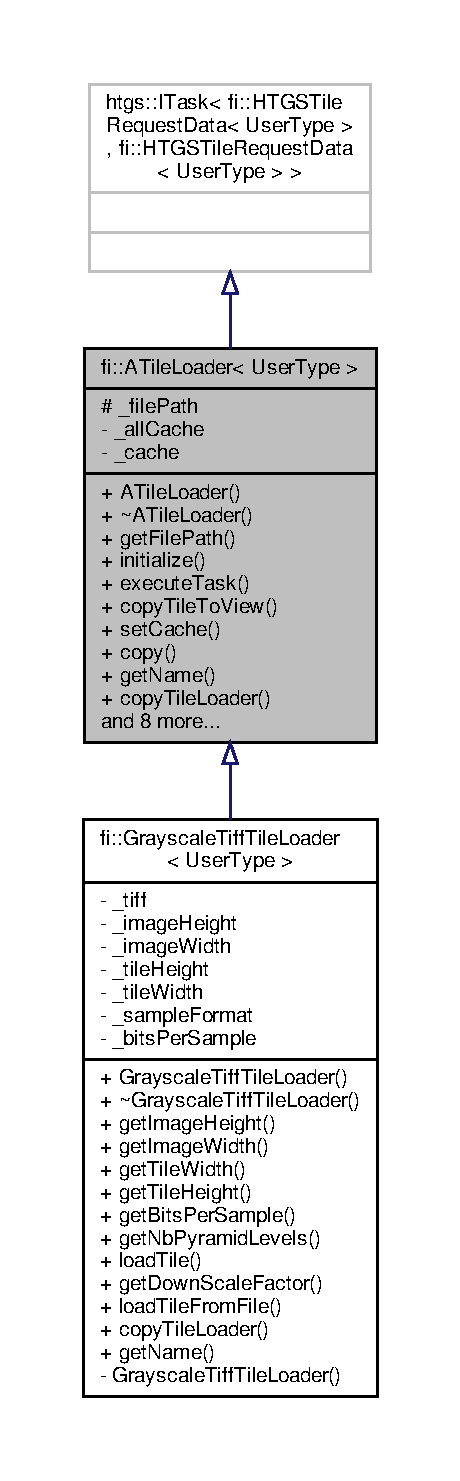
\includegraphics[height=550pt]{d0/d13/classfi_1_1ATileLoader__inherit__graph}
\end{center}
\end{figure}


Collaboration diagram for fi\+:\+:A\+Tile\+Loader$<$ User\+Type $>$\+:
\nopagebreak
\begin{figure}[H]
\begin{center}
\leavevmode
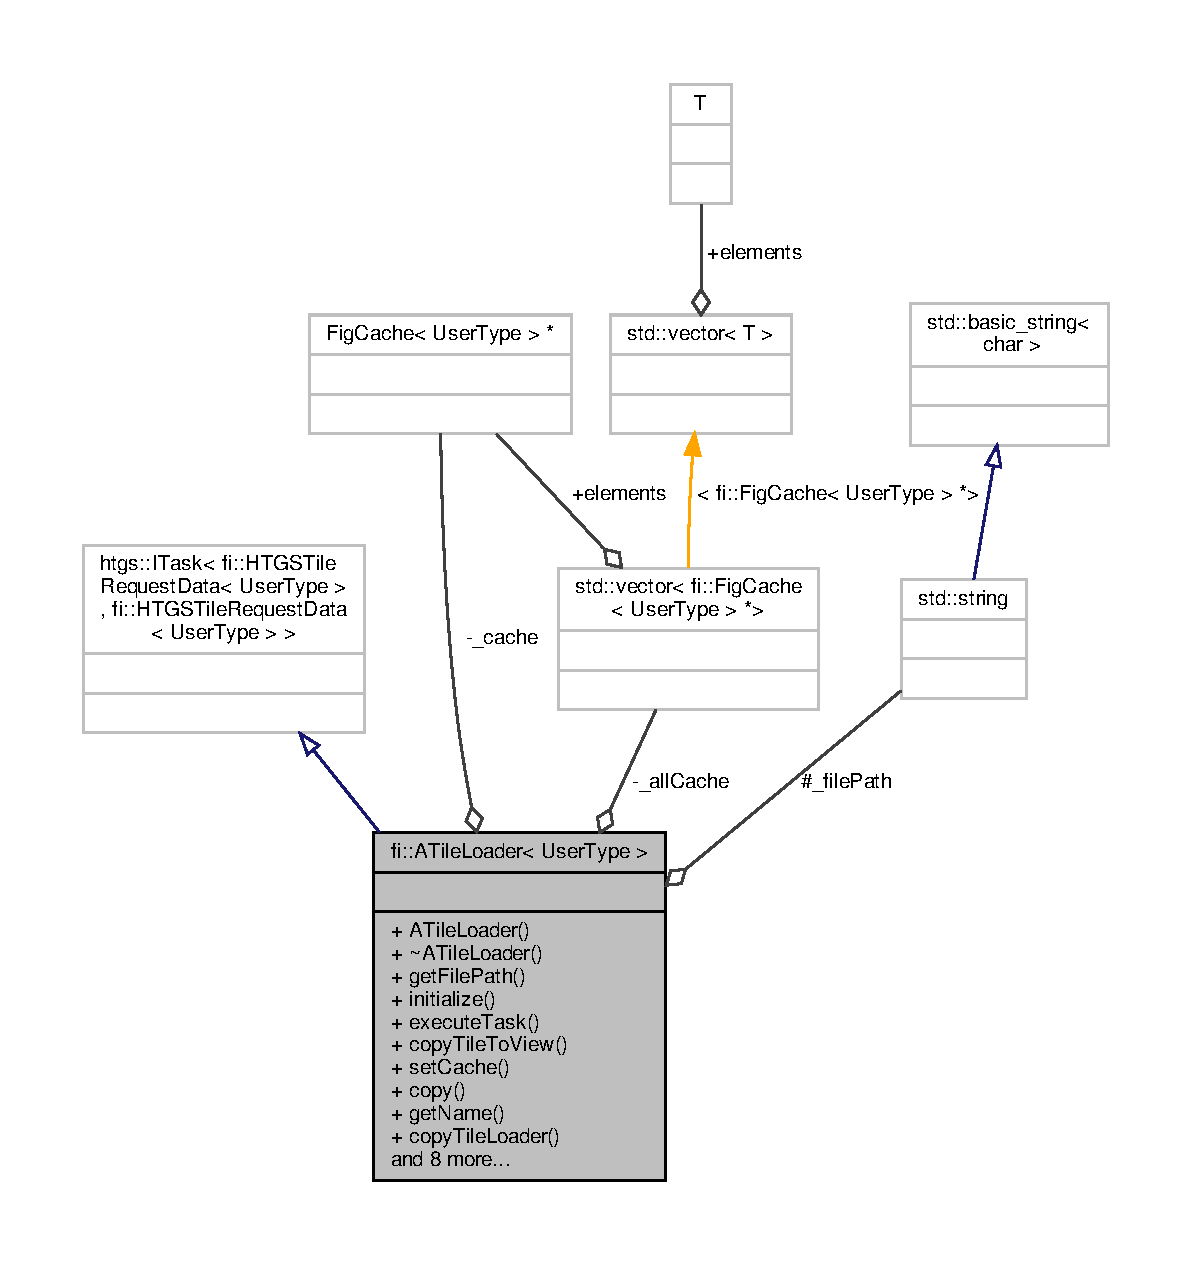
\includegraphics[width=350pt]{d6/deb/classfi_1_1ATileLoader__coll__graph}
\end{center}
\end{figure}
\subsection*{Public Member Functions}
\begin{DoxyCompactItemize}
\item 
\hyperlink{classfi_1_1ATileLoader_a853a3209bab3a5e024f9d1ca7c8933f3}{A\+Tile\+Loader} (std\+::string file\+Path, size\+\_\+t num\+Threads=1)
\begin{DoxyCompactList}\small\item\em Any Tile loader default constructor. \end{DoxyCompactList}\item 
\hyperlink{classfi_1_1ATileLoader_ab04d8b3add3187cfa57a0f5323f8f7b4}{$\sim$\+A\+Tile\+Loader} ()=default
\begin{DoxyCompactList}\small\item\em Default destructor. \end{DoxyCompactList}\item 
const std\+::string \& \hyperlink{classfi_1_1ATileLoader_a5efe3a55a89531b4ef657e58e5753340}{get\+File\+Path} () const
\begin{DoxyCompactList}\small\item\em Get File path. \end{DoxyCompactList}\item 
void \hyperlink{classfi_1_1ATileLoader_a12929a1a82ff9cf2615e7a7420ba92c4}{initialize} () final
\begin{DoxyCompactList}\small\item\em Initialize function. \end{DoxyCompactList}\item 
void \hyperlink{classfi_1_1ATileLoader_ab3fb2e90d11d160e89c6b8a7df684c7f}{execute\+Task} (std\+::shared\+\_\+ptr$<$ \hyperlink{classfi_1_1HTGSTileRequestData}{fi\+::\+H\+T\+G\+S\+Tile\+Request\+Data}$<$ User\+Type $>$$>$ tile\+Request\+Data) final
\begin{DoxyCompactList}\small\item\em Load a tile from a file, populate the current view, and send the view to the view counter. \end{DoxyCompactList}\item 
void \hyperlink{classfi_1_1ATileLoader_a69b1eaf0e9f636f756f514bd985a4cb5}{copy\+Tile\+To\+View} (std\+::shared\+\_\+ptr$<$ \hyperlink{classfi_1_1HTGSTileRequestData}{fi\+::\+H\+T\+G\+S\+Tile\+Request\+Data}$<$ User\+Type $>$$>$ tile\+Request\+Data, \hyperlink{classfi_1_1CachedTile}{Cached\+Tile}$<$ User\+Type $>$ $\ast$cached\+Tile)
\begin{DoxyCompactList}\small\item\em Copy (part of or all) the cached tile to the view. \end{DoxyCompactList}\item 
void \hyperlink{classfi_1_1ATileLoader_a1113a06fc88a278bede14bbee2ae4a59}{set\+Cache} (std\+::vector$<$ \hyperlink{classfi_1_1FigCache}{fi\+::\+Fig\+Cache}$<$ User\+Type $>$ $\ast$$>$ \&all\+Cache)
\begin{DoxyCompactList}\small\item\em Set the caches. \end{DoxyCompactList}\item 
\hyperlink{classfi_1_1ATileLoader}{A\+Tile\+Loader} $\ast$ \hyperlink{classfi_1_1ATileLoader_a6f842aefc3db84a1c95edaa9f550c1e7}{copy} () final
\begin{DoxyCompactList}\small\item\em \hyperlink{classfi_1_1ATileLoader}{A\+Tile\+Loader} copy function used by H\+T\+GS to create a new \hyperlink{classfi_1_1ATileLoader}{A\+Tile\+Loader}, will call copy\+Tile\+Loader more specialize. \end{DoxyCompactList}\item 
std\+::string \hyperlink{classfi_1_1ATileLoader_abb4cad235d57fbfb29ff5d37caf32a62}{get\+Name} () override=0
\begin{DoxyCompactList}\small\item\em Get task name. \end{DoxyCompactList}\item 
virtual \hyperlink{classfi_1_1ATileLoader}{A\+Tile\+Loader} $\ast$ \hyperlink{classfi_1_1ATileLoader_a99bd30a8283474c5bf667054a83a008d}{copy\+Tile\+Loader} ()=0
\begin{DoxyCompactList}\small\item\em Copy Function. \end{DoxyCompactList}\item 
virtual uint32\+\_\+t \hyperlink{classfi_1_1ATileLoader_a53fb257d3ec8f3fa3d5f6c58de859000}{get\+Image\+Height} (uint32\+\_\+t level=0) const =0
\begin{DoxyCompactList}\small\item\em Getter to image Height. \end{DoxyCompactList}\item 
virtual uint32\+\_\+t \hyperlink{classfi_1_1ATileLoader_ad775bcbdddf7da6bb3f857a53c075a86}{get\+Image\+Width} (uint32\+\_\+t level=0) const =0
\begin{DoxyCompactList}\small\item\em Getter to image Width. \end{DoxyCompactList}\item 
virtual uint32\+\_\+t \hyperlink{classfi_1_1ATileLoader_ad4ced663628b4134fd8f7bb0cfd2a652}{get\+Tile\+Width} (uint32\+\_\+t level=0) const =0
\begin{DoxyCompactList}\small\item\em Getter to tile Width. \end{DoxyCompactList}\item 
virtual uint32\+\_\+t \hyperlink{classfi_1_1ATileLoader_a531ceb7c73457fdde7055e95abd777fa}{get\+Tile\+Height} (uint32\+\_\+t level=0) const =0
\begin{DoxyCompactList}\small\item\em Getter to tile Height. \end{DoxyCompactList}\item 
virtual short \hyperlink{classfi_1_1ATileLoader_a20ce7ee013801a64dedc95c2a3b9be7f}{get\+Bits\+Per\+Sample} () const =0
\begin{DoxyCompactList}\small\item\em Get file bits per samples. \end{DoxyCompactList}\item 
virtual uint32\+\_\+t \hyperlink{classfi_1_1ATileLoader_ad6550495be22454b5f72d46c68622c37}{get\+Nb\+Pyramid\+Levels} () const =0
\begin{DoxyCompactList}\small\item\em Get number of pyramid levels. \end{DoxyCompactList}\item 
virtual float \hyperlink{classfi_1_1ATileLoader_a07d565eeaa7076d905a329c80c1e980c}{get\+Down\+Scale\+Factor} (uint32\+\_\+t level=0)
\begin{DoxyCompactList}\small\item\em Get the down scalar factor for a specific pyramid level. \end{DoxyCompactList}\item 
virtual double \hyperlink{classfi_1_1ATileLoader_a46d85c52fe89339a3ffbc1cb9c377eb0}{load\+Tile\+From\+File} (User\+Type $\ast$tile, uint32\+\_\+t index\+Row\+Global\+Tile, uint32\+\_\+t index\+Col\+Global\+Tile)=0
\begin{DoxyCompactList}\small\item\em Load a specific Tile at 0 based indexes (index\+Row\+Global\+Tile, index\+Col\+Global\+Tile) of size tile\+Height x tile\+Width. \end{DoxyCompactList}\end{DoxyCompactItemize}
\subsection*{Protected Attributes}
\begin{DoxyCompactItemize}
\item 
std\+::string \hyperlink{classfi_1_1ATileLoader_aa96fb4d90ac425c4b670b23f6ebe49f6}{\+\_\+file\+Path}
\begin{DoxyCompactList}\small\item\em Path to file to load. \end{DoxyCompactList}\end{DoxyCompactItemize}
\subsection*{Private Attributes}
\begin{DoxyCompactItemize}
\item 
std\+::vector$<$ \hyperlink{classfi_1_1FigCache}{fi\+::\+Fig\+Cache}$<$ User\+Type $>$ $\ast$ $>$ \hyperlink{classfi_1_1ATileLoader_a07679e26c08c1f998e00cdf3e1af5d43}{\+\_\+all\+Cache}
\begin{DoxyCompactList}\small\item\em All caches for each pyramid levels. \end{DoxyCompactList}\item 
\hyperlink{classfi_1_1FigCache}{Fig\+Cache}$<$ User\+Type $>$ $\ast$ \hyperlink{classfi_1_1ATileLoader_a35c8ba6cc53333935c03d822b24095b9}{\+\_\+cache} = nullptr
\begin{DoxyCompactList}\small\item\em Tile Cache. \end{DoxyCompactList}\end{DoxyCompactItemize}


\subsection{Detailed Description}
\subsubsection*{template$<$typename User\+Type$>$\newline
class fi\+::\+A\+Tile\+Loader$<$ User\+Type $>$}

Tile Loader interface. 

Can\textquotesingle{}t be instantiate. Take a \hyperlink{classfi_1_1HTGSTileRequestData}{H\+T\+G\+S\+Tile\+Request\+Data} and produce a htgs\+::\+Memory\+Data$<$\+View\+Data$>$$>$. Has to be inherited to create a new tile loader. The new Tile loader has to override and implement the following functions\+: 
\begin{DoxyCode}
\textcolor{keyword}{virtual} std::string \hyperlink{classfi_1_1ATileLoader_abb4cad235d57fbfb29ff5d37caf32a62}{getName}() = 0;
\textcolor{keyword}{virtual} \hyperlink{classfi_1_1ATileLoader_a853a3209bab3a5e024f9d1ca7c8933f3}{ATileLoader} *\hyperlink{classfi_1_1ATileLoader_a99bd30a8283474c5bf667054a83a008d}{copyTileLoader}() = 0;
\textcolor{keyword}{virtual} uint32\_t \hyperlink{classfi_1_1ATileLoader_a53fb257d3ec8f3fa3d5f6c58de859000}{getImageHeight}(uint32\_t level = 0) \textcolor{keyword}{const} = 0;
\textcolor{keyword}{virtual} uint32\_t \hyperlink{classfi_1_1ATileLoader_ad775bcbdddf7da6bb3f857a53c075a86}{getImageWidth}(uint32\_t level = 0) \textcolor{keyword}{const} = 0;
\textcolor{keyword}{virtual} uint32\_t \hyperlink{classfi_1_1ATileLoader_ad4ced663628b4134fd8f7bb0cfd2a652}{getTileWidth}(uint32\_t level = 0) \textcolor{keyword}{const} = 0;
\textcolor{keyword}{virtual} uint32\_t \hyperlink{classfi_1_1ATileLoader_a531ceb7c73457fdde7055e95abd777fa}{getTileHeight}(uint32\_t level = 0) \textcolor{keyword}{const} = 0;
\textcolor{keyword}{virtual} \textcolor{keywordtype}{short} \hyperlink{classfi_1_1ATileLoader_a20ce7ee013801a64dedc95c2a3b9be7f}{getBitsPerSample}() \textcolor{keyword}{const} = 0;
\textcolor{keyword}{virtual} uint32\_t \hyperlink{classfi_1_1ATileLoader_ad6550495be22454b5f72d46c68622c37}{getNbPyramidLevels}() \textcolor{keyword}{const} = 0;
\textcolor{keyword}{virtual} \textcolor{keywordtype}{double} \hyperlink{classfi_1_1ATileLoader_a46d85c52fe89339a3ffbc1cb9c377eb0}{loadTileFromFile}(UserType *tile, uint32\_t
    indexRowGlobalTile, uint32\_t indexColGlobalTile) = 0;
\end{DoxyCode}
 and has to set the \+\_\+bits\+Per\+Sample protected attribute. The overloaded copy function should also copy the following\+: \+\_\+cache / \+\_\+file\+Path / \+\_\+bits\+Per\+Sample / num\+Threads, which can be taken from the available getters. 
\begin{DoxyTemplParams}{Template Parameters}
{\em User\+Type} & Data Type wanted by the user, which is stored within a \hyperlink{classfi_1_1View}{fi\+::\+View} \\
\hline
\end{DoxyTemplParams}


Definition at line 73 of file A\+Tile\+Loader.\+h.



\subsection{Constructor \& Destructor Documentation}
\mbox{\Hypertarget{classfi_1_1ATileLoader_a853a3209bab3a5e024f9d1ca7c8933f3}\label{classfi_1_1ATileLoader_a853a3209bab3a5e024f9d1ca7c8933f3}} 
\index{fi\+::\+A\+Tile\+Loader@{fi\+::\+A\+Tile\+Loader}!A\+Tile\+Loader@{A\+Tile\+Loader}}
\index{A\+Tile\+Loader@{A\+Tile\+Loader}!fi\+::\+A\+Tile\+Loader@{fi\+::\+A\+Tile\+Loader}}
\subsubsection{\texorpdfstring{A\+Tile\+Loader()}{ATileLoader()}}
{\footnotesize\ttfamily template$<$typename User\+Type$>$ \\
\hyperlink{classfi_1_1ATileLoader}{fi\+::\+A\+Tile\+Loader}$<$ User\+Type $>$\+::\hyperlink{classfi_1_1ATileLoader}{A\+Tile\+Loader} (\begin{DoxyParamCaption}\item[{std\+::string}]{file\+Path,  }\item[{size\+\_\+t}]{num\+Threads = {\ttfamily 1} }\end{DoxyParamCaption})\hspace{0.3cm}{\ttfamily [inline]}, {\ttfamily [explicit]}}



Any Tile loader default constructor. 


\begin{DoxyParams}{Parameters}
{\em file\+Path} & File path \\
\hline
{\em num\+Threads} & number of threads used by the tile loader \\
\hline
\end{DoxyParams}


Definition at line 79 of file A\+Tile\+Loader.\+h.

Here is the call graph for this function\+:
\nopagebreak
\begin{figure}[H]
\begin{center}
\leavevmode
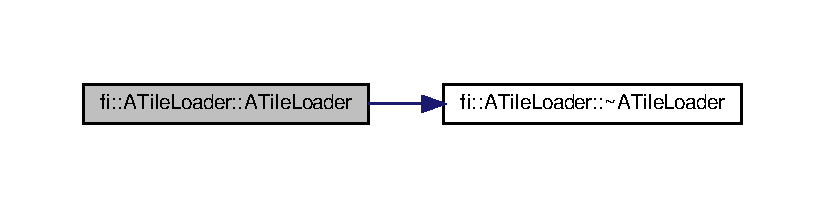
\includegraphics[width=350pt]{dc/d54/classfi_1_1ATileLoader_a853a3209bab3a5e024f9d1ca7c8933f3_cgraph}
\end{center}
\end{figure}
\mbox{\Hypertarget{classfi_1_1ATileLoader_ab04d8b3add3187cfa57a0f5323f8f7b4}\label{classfi_1_1ATileLoader_ab04d8b3add3187cfa57a0f5323f8f7b4}} 
\index{fi\+::\+A\+Tile\+Loader@{fi\+::\+A\+Tile\+Loader}!````~A\+Tile\+Loader@{$\sim$\+A\+Tile\+Loader}}
\index{````~A\+Tile\+Loader@{$\sim$\+A\+Tile\+Loader}!fi\+::\+A\+Tile\+Loader@{fi\+::\+A\+Tile\+Loader}}
\subsubsection{\texorpdfstring{$\sim$\+A\+Tile\+Loader()}{~ATileLoader()}}
{\footnotesize\ttfamily template$<$typename User\+Type$>$ \\
\hyperlink{classfi_1_1ATileLoader}{fi\+::\+A\+Tile\+Loader}$<$ User\+Type $>$\+::$\sim$\hyperlink{classfi_1_1ATileLoader}{A\+Tile\+Loader} (\begin{DoxyParamCaption}{ }\end{DoxyParamCaption})\hspace{0.3cm}{\ttfamily [default]}}



Default destructor. 

Here is the caller graph for this function\+:
\nopagebreak
\begin{figure}[H]
\begin{center}
\leavevmode
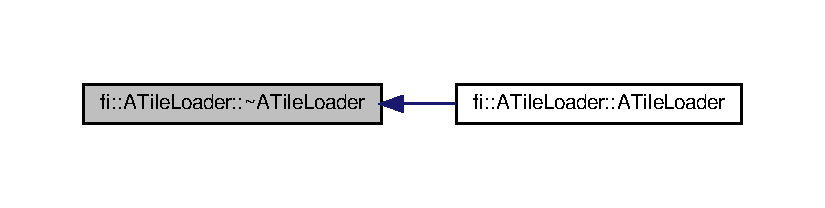
\includegraphics[width=350pt]{dc/d54/classfi_1_1ATileLoader_ab04d8b3add3187cfa57a0f5323f8f7b4_icgraph}
\end{center}
\end{figure}


\subsection{Member Function Documentation}
\mbox{\Hypertarget{classfi_1_1ATileLoader_a6f842aefc3db84a1c95edaa9f550c1e7}\label{classfi_1_1ATileLoader_a6f842aefc3db84a1c95edaa9f550c1e7}} 
\index{fi\+::\+A\+Tile\+Loader@{fi\+::\+A\+Tile\+Loader}!copy@{copy}}
\index{copy@{copy}!fi\+::\+A\+Tile\+Loader@{fi\+::\+A\+Tile\+Loader}}
\subsubsection{\texorpdfstring{copy()}{copy()}}
{\footnotesize\ttfamily template$<$typename User\+Type$>$ \\
\hyperlink{classfi_1_1ATileLoader}{A\+Tile\+Loader}$\ast$ \hyperlink{classfi_1_1ATileLoader}{fi\+::\+A\+Tile\+Loader}$<$ User\+Type $>$\+::copy (\begin{DoxyParamCaption}{ }\end{DoxyParamCaption})\hspace{0.3cm}{\ttfamily [inline]}, {\ttfamily [final]}}



\hyperlink{classfi_1_1ATileLoader}{A\+Tile\+Loader} copy function used by H\+T\+GS to create a new \hyperlink{classfi_1_1ATileLoader}{A\+Tile\+Loader}, will call copy\+Tile\+Loader more specialize. 

\begin{DoxyReturn}{Returns}
\hyperlink{classfi_1_1ATileLoader}{A\+Tile\+Loader} copied 
\end{DoxyReturn}


Definition at line 165 of file A\+Tile\+Loader.\+h.

Here is the call graph for this function\+:
\nopagebreak
\begin{figure}[H]
\begin{center}
\leavevmode
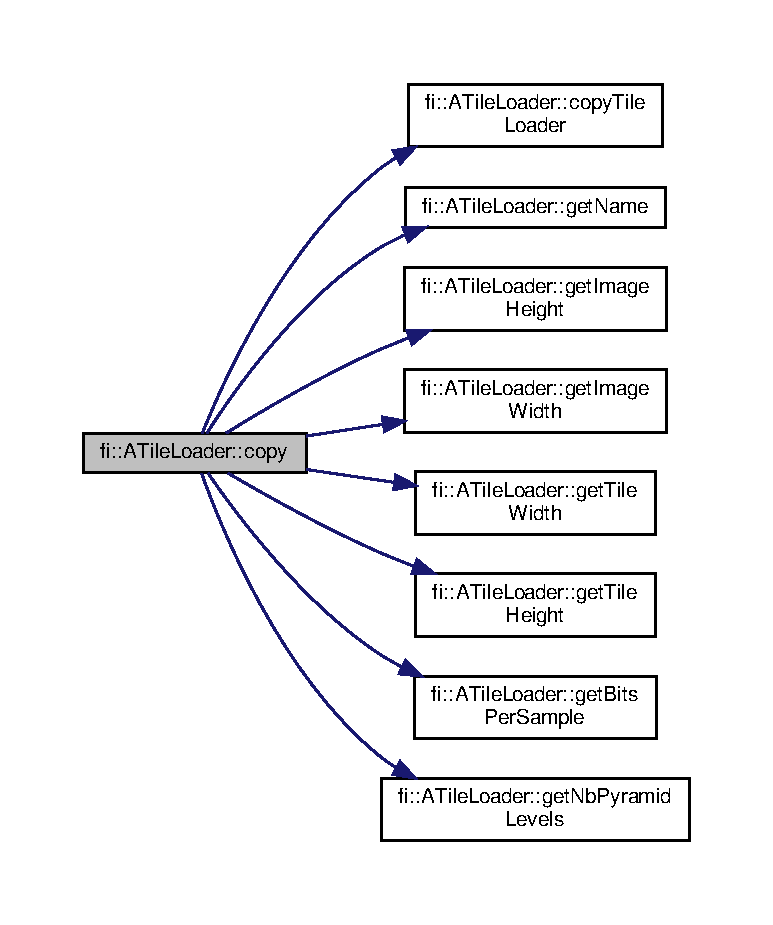
\includegraphics[width=350pt]{dc/d54/classfi_1_1ATileLoader_a6f842aefc3db84a1c95edaa9f550c1e7_cgraph}
\end{center}
\end{figure}
\mbox{\Hypertarget{classfi_1_1ATileLoader_a99bd30a8283474c5bf667054a83a008d}\label{classfi_1_1ATileLoader_a99bd30a8283474c5bf667054a83a008d}} 
\index{fi\+::\+A\+Tile\+Loader@{fi\+::\+A\+Tile\+Loader}!copy\+Tile\+Loader@{copy\+Tile\+Loader}}
\index{copy\+Tile\+Loader@{copy\+Tile\+Loader}!fi\+::\+A\+Tile\+Loader@{fi\+::\+A\+Tile\+Loader}}
\subsubsection{\texorpdfstring{copy\+Tile\+Loader()}{copyTileLoader()}}
{\footnotesize\ttfamily template$<$typename User\+Type$>$ \\
virtual \hyperlink{classfi_1_1ATileLoader}{A\+Tile\+Loader}$\ast$ \hyperlink{classfi_1_1ATileLoader}{fi\+::\+A\+Tile\+Loader}$<$ User\+Type $>$\+::copy\+Tile\+Loader (\begin{DoxyParamCaption}{ }\end{DoxyParamCaption})\hspace{0.3cm}{\ttfamily [pure virtual]}}



Copy Function. 

\begin{DoxyReturn}{Returns}
\hyperlink{classfi_1_1ATileLoader}{A\+Tile\+Loader} copied 
\end{DoxyReturn}


Implemented in \hyperlink{classfi_1_1GrayscaleTiffTileLoader_a57eb82e8bcdf71d2cd5f16f93bbe24a4}{fi\+::\+Grayscale\+Tiff\+Tile\+Loader$<$ User\+Type $>$}.

Here is the caller graph for this function\+:
\nopagebreak
\begin{figure}[H]
\begin{center}
\leavevmode
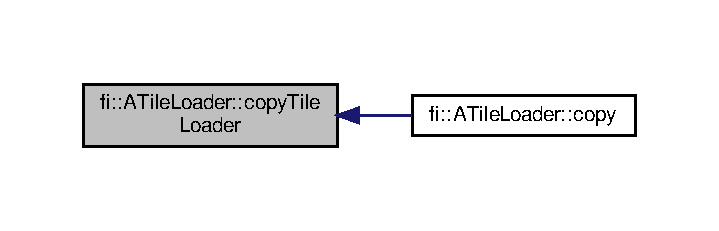
\includegraphics[width=345pt]{dc/d54/classfi_1_1ATileLoader_a99bd30a8283474c5bf667054a83a008d_icgraph}
\end{center}
\end{figure}
\mbox{\Hypertarget{classfi_1_1ATileLoader_a69b1eaf0e9f636f756f514bd985a4cb5}\label{classfi_1_1ATileLoader_a69b1eaf0e9f636f756f514bd985a4cb5}} 
\index{fi\+::\+A\+Tile\+Loader@{fi\+::\+A\+Tile\+Loader}!copy\+Tile\+To\+View@{copy\+Tile\+To\+View}}
\index{copy\+Tile\+To\+View@{copy\+Tile\+To\+View}!fi\+::\+A\+Tile\+Loader@{fi\+::\+A\+Tile\+Loader}}
\subsubsection{\texorpdfstring{copy\+Tile\+To\+View()}{copyTileToView()}}
{\footnotesize\ttfamily template$<$typename User\+Type$>$ \\
void \hyperlink{classfi_1_1ATileLoader}{fi\+::\+A\+Tile\+Loader}$<$ User\+Type $>$\+::copy\+Tile\+To\+View (\begin{DoxyParamCaption}\item[{std\+::shared\+\_\+ptr$<$ \hyperlink{classfi_1_1HTGSTileRequestData}{fi\+::\+H\+T\+G\+S\+Tile\+Request\+Data}$<$ User\+Type $>$$>$}]{tile\+Request\+Data,  }\item[{\hyperlink{classfi_1_1CachedTile}{Cached\+Tile}$<$ User\+Type $>$ $\ast$}]{cached\+Tile }\end{DoxyParamCaption})\hspace{0.3cm}{\ttfamily [inline]}}



Copy (part of or all) the cached tile to the view. 


\begin{DoxyParams}{Parameters}
{\em tile\+Request\+Data} & Destination tile request \\
\hline
{\em cached\+Tile} & Source cached tile \\
\hline
\end{DoxyParams}


Definition at line 131 of file A\+Tile\+Loader.\+h.

Here is the call graph for this function\+:
\nopagebreak
\begin{figure}[H]
\begin{center}
\leavevmode
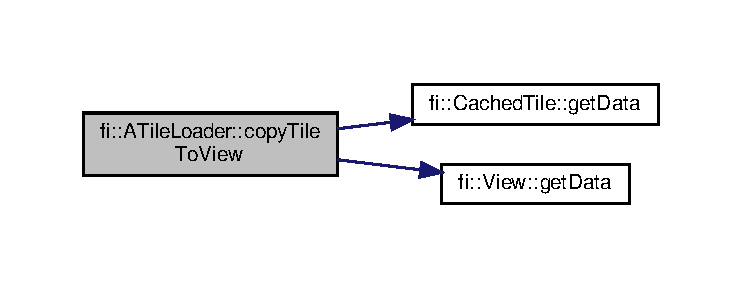
\includegraphics[width=350pt]{dc/d54/classfi_1_1ATileLoader_a69b1eaf0e9f636f756f514bd985a4cb5_cgraph}
\end{center}
\end{figure}
Here is the caller graph for this function\+:
\nopagebreak
\begin{figure}[H]
\begin{center}
\leavevmode
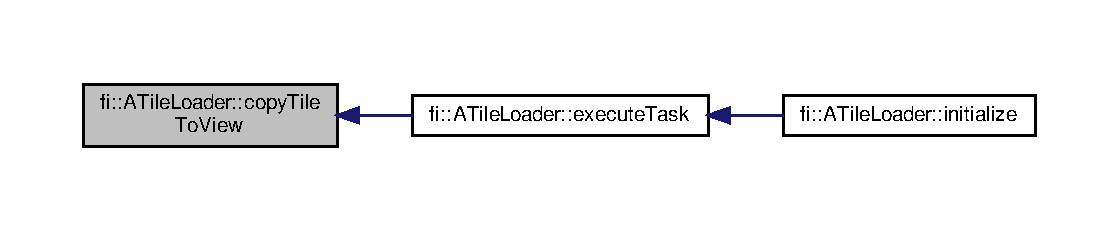
\includegraphics[width=350pt]{dc/d54/classfi_1_1ATileLoader_a69b1eaf0e9f636f756f514bd985a4cb5_icgraph}
\end{center}
\end{figure}
\mbox{\Hypertarget{classfi_1_1ATileLoader_ab3fb2e90d11d160e89c6b8a7df684c7f}\label{classfi_1_1ATileLoader_ab3fb2e90d11d160e89c6b8a7df684c7f}} 
\index{fi\+::\+A\+Tile\+Loader@{fi\+::\+A\+Tile\+Loader}!execute\+Task@{execute\+Task}}
\index{execute\+Task@{execute\+Task}!fi\+::\+A\+Tile\+Loader@{fi\+::\+A\+Tile\+Loader}}
\subsubsection{\texorpdfstring{execute\+Task()}{executeTask()}}
{\footnotesize\ttfamily template$<$typename User\+Type$>$ \\
void \hyperlink{classfi_1_1ATileLoader}{fi\+::\+A\+Tile\+Loader}$<$ User\+Type $>$\+::execute\+Task (\begin{DoxyParamCaption}\item[{std\+::shared\+\_\+ptr$<$ \hyperlink{classfi_1_1HTGSTileRequestData}{fi\+::\+H\+T\+G\+S\+Tile\+Request\+Data}$<$ User\+Type $>$$>$}]{tile\+Request\+Data }\end{DoxyParamCaption})\hspace{0.3cm}{\ttfamily [inline]}, {\ttfamily [final]}}



Load a tile from a file, populate the current view, and send the view to the view counter. 

Processes the requested tile by first checking the cache, if it is not in the cache, then the tile is loaded from the disk. The data is copied into a \hyperlink{classfi_1_1View}{fi\+::\+View} and sent to the view counter. 
\begin{DoxyParams}{Parameters}
{\em tile\+Request\+Data} & the requested tile to load \\
\hline
\end{DoxyParams}


Definition at line 106 of file A\+Tile\+Loader.\+h.

Here is the call graph for this function\+:
\nopagebreak
\begin{figure}[H]
\begin{center}
\leavevmode
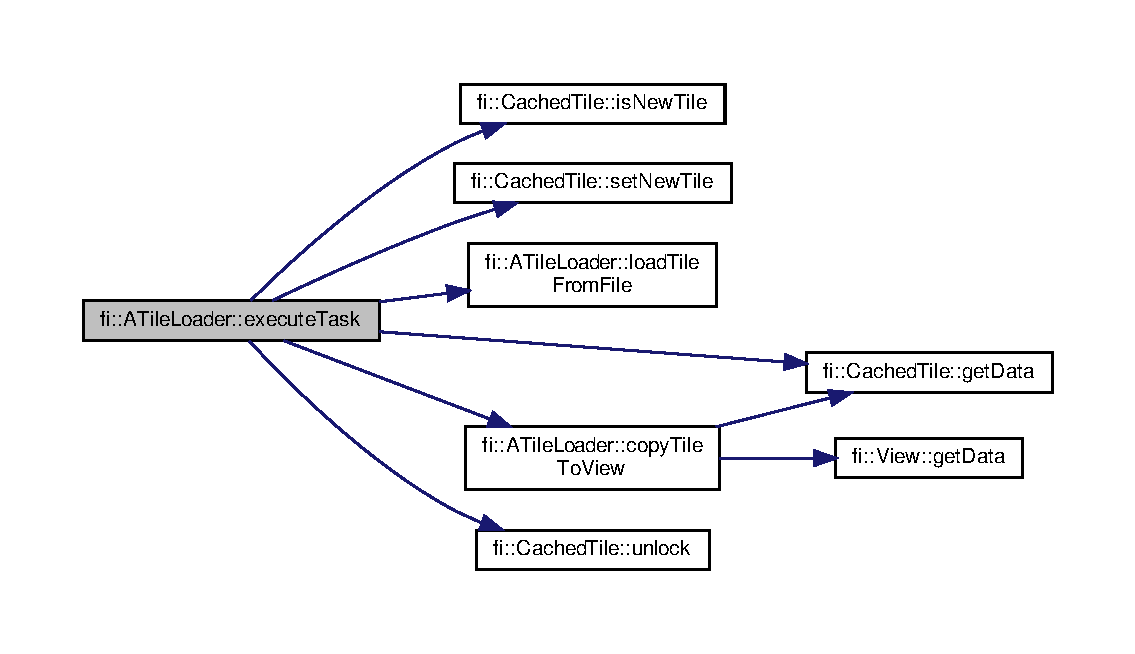
\includegraphics[width=350pt]{dc/d54/classfi_1_1ATileLoader_ab3fb2e90d11d160e89c6b8a7df684c7f_cgraph}
\end{center}
\end{figure}
Here is the caller graph for this function\+:
\nopagebreak
\begin{figure}[H]
\begin{center}
\leavevmode
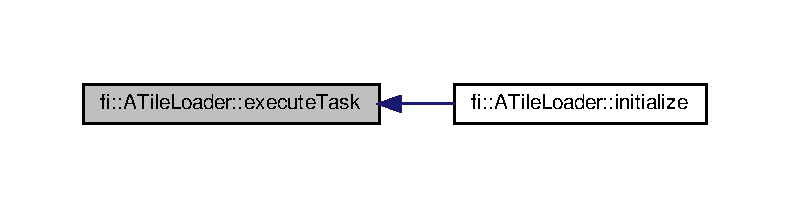
\includegraphics[width=350pt]{dc/d54/classfi_1_1ATileLoader_ab3fb2e90d11d160e89c6b8a7df684c7f_icgraph}
\end{center}
\end{figure}
\mbox{\Hypertarget{classfi_1_1ATileLoader_a20ce7ee013801a64dedc95c2a3b9be7f}\label{classfi_1_1ATileLoader_a20ce7ee013801a64dedc95c2a3b9be7f}} 
\index{fi\+::\+A\+Tile\+Loader@{fi\+::\+A\+Tile\+Loader}!get\+Bits\+Per\+Sample@{get\+Bits\+Per\+Sample}}
\index{get\+Bits\+Per\+Sample@{get\+Bits\+Per\+Sample}!fi\+::\+A\+Tile\+Loader@{fi\+::\+A\+Tile\+Loader}}
\subsubsection{\texorpdfstring{get\+Bits\+Per\+Sample()}{getBitsPerSample()}}
{\footnotesize\ttfamily template$<$typename User\+Type$>$ \\
virtual short \hyperlink{classfi_1_1ATileLoader}{fi\+::\+A\+Tile\+Loader}$<$ User\+Type $>$\+::get\+Bits\+Per\+Sample (\begin{DoxyParamCaption}{ }\end{DoxyParamCaption}) const\hspace{0.3cm}{\ttfamily [pure virtual]}}



Get file bits per samples. 

\begin{DoxyReturn}{Returns}
File bits per sample 
\end{DoxyReturn}


Implemented in \hyperlink{classfi_1_1GrayscaleTiffTileLoader_a80ae5ca350571d2c993a68d40bdc39c9}{fi\+::\+Grayscale\+Tiff\+Tile\+Loader$<$ User\+Type $>$}.

Here is the caller graph for this function\+:
\nopagebreak
\begin{figure}[H]
\begin{center}
\leavevmode
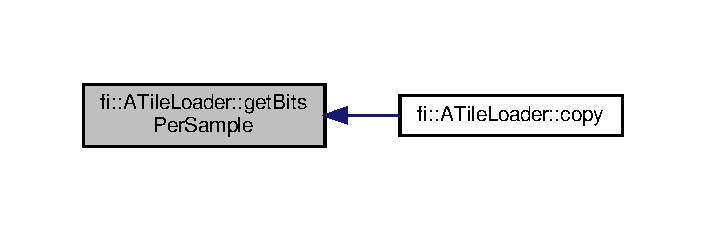
\includegraphics[width=339pt]{dc/d54/classfi_1_1ATileLoader_a20ce7ee013801a64dedc95c2a3b9be7f_icgraph}
\end{center}
\end{figure}
\mbox{\Hypertarget{classfi_1_1ATileLoader_a07d565eeaa7076d905a329c80c1e980c}\label{classfi_1_1ATileLoader_a07d565eeaa7076d905a329c80c1e980c}} 
\index{fi\+::\+A\+Tile\+Loader@{fi\+::\+A\+Tile\+Loader}!get\+Down\+Scale\+Factor@{get\+Down\+Scale\+Factor}}
\index{get\+Down\+Scale\+Factor@{get\+Down\+Scale\+Factor}!fi\+::\+A\+Tile\+Loader@{fi\+::\+A\+Tile\+Loader}}
\subsubsection{\texorpdfstring{get\+Down\+Scale\+Factor()}{getDownScaleFactor()}}
{\footnotesize\ttfamily template$<$typename User\+Type$>$ \\
virtual float \hyperlink{classfi_1_1ATileLoader}{fi\+::\+A\+Tile\+Loader}$<$ User\+Type $>$\+::get\+Down\+Scale\+Factor (\begin{DoxyParamCaption}\item[{uint32\+\_\+t}]{level = {\ttfamily 0} }\end{DoxyParamCaption})\hspace{0.3cm}{\ttfamily [inline]}, {\ttfamily [virtual]}}



Get the down scalar factor for a specific pyramid level. 


\begin{DoxyParams}{Parameters}
{\em level} & Pyramid level \\
\hline
\end{DoxyParams}
\begin{DoxyReturn}{Returns}
The down scalar factor for a specific pyramid level 
\end{DoxyReturn}


Reimplemented in \hyperlink{classfi_1_1GrayscaleTiffTileLoader_a30200666aa71f80ea0fa9e035519635b}{fi\+::\+Grayscale\+Tiff\+Tile\+Loader$<$ User\+Type $>$}.



Definition at line 207 of file A\+Tile\+Loader.\+h.

Here is the call graph for this function\+:
\nopagebreak
\begin{figure}[H]
\begin{center}
\leavevmode
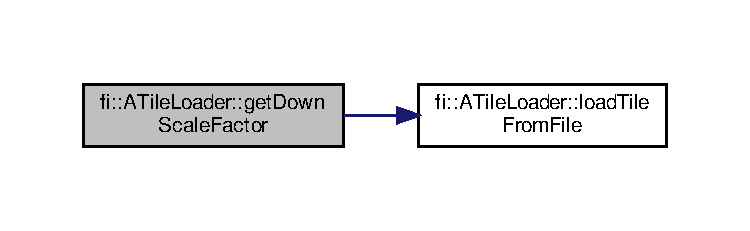
\includegraphics[width=350pt]{dc/d54/classfi_1_1ATileLoader_a07d565eeaa7076d905a329c80c1e980c_cgraph}
\end{center}
\end{figure}
\mbox{\Hypertarget{classfi_1_1ATileLoader_a5efe3a55a89531b4ef657e58e5753340}\label{classfi_1_1ATileLoader_a5efe3a55a89531b4ef657e58e5753340}} 
\index{fi\+::\+A\+Tile\+Loader@{fi\+::\+A\+Tile\+Loader}!get\+File\+Path@{get\+File\+Path}}
\index{get\+File\+Path@{get\+File\+Path}!fi\+::\+A\+Tile\+Loader@{fi\+::\+A\+Tile\+Loader}}
\subsubsection{\texorpdfstring{get\+File\+Path()}{getFilePath()}}
{\footnotesize\ttfamily template$<$typename User\+Type$>$ \\
const std\+::string\& \hyperlink{classfi_1_1ATileLoader}{fi\+::\+A\+Tile\+Loader}$<$ User\+Type $>$\+::get\+File\+Path (\begin{DoxyParamCaption}{ }\end{DoxyParamCaption}) const\hspace{0.3cm}{\ttfamily [inline]}}



Get File path. 

\begin{DoxyReturn}{Returns}
File path 
\end{DoxyReturn}


Definition at line 89 of file A\+Tile\+Loader.\+h.

Here is the caller graph for this function\+:
\nopagebreak
\begin{figure}[H]
\begin{center}
\leavevmode
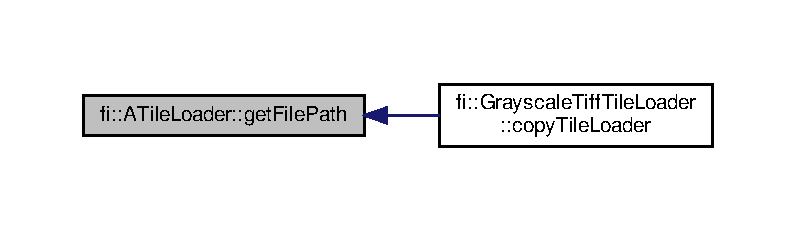
\includegraphics[width=350pt]{dc/d54/classfi_1_1ATileLoader_a5efe3a55a89531b4ef657e58e5753340_icgraph}
\end{center}
\end{figure}
\mbox{\Hypertarget{classfi_1_1ATileLoader_a53fb257d3ec8f3fa3d5f6c58de859000}\label{classfi_1_1ATileLoader_a53fb257d3ec8f3fa3d5f6c58de859000}} 
\index{fi\+::\+A\+Tile\+Loader@{fi\+::\+A\+Tile\+Loader}!get\+Image\+Height@{get\+Image\+Height}}
\index{get\+Image\+Height@{get\+Image\+Height}!fi\+::\+A\+Tile\+Loader@{fi\+::\+A\+Tile\+Loader}}
\subsubsection{\texorpdfstring{get\+Image\+Height()}{getImageHeight()}}
{\footnotesize\ttfamily template$<$typename User\+Type$>$ \\
virtual uint32\+\_\+t \hyperlink{classfi_1_1ATileLoader}{fi\+::\+A\+Tile\+Loader}$<$ User\+Type $>$\+::get\+Image\+Height (\begin{DoxyParamCaption}\item[{uint32\+\_\+t}]{level = {\ttfamily 0} }\end{DoxyParamCaption}) const\hspace{0.3cm}{\ttfamily [pure virtual]}}



Getter to image Height. 

\begin{DoxyReturn}{Returns}
Image height 
\end{DoxyReturn}


Implemented in \hyperlink{classfi_1_1GrayscaleTiffTileLoader_aedb905b521b888c68a59d20695c33e51}{fi\+::\+Grayscale\+Tiff\+Tile\+Loader$<$ User\+Type $>$}.

Here is the caller graph for this function\+:
\nopagebreak
\begin{figure}[H]
\begin{center}
\leavevmode
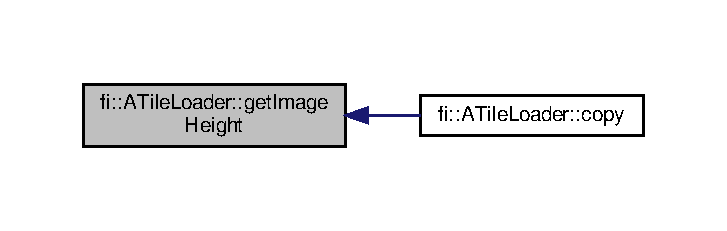
\includegraphics[width=349pt]{dc/d54/classfi_1_1ATileLoader_a53fb257d3ec8f3fa3d5f6c58de859000_icgraph}
\end{center}
\end{figure}
\mbox{\Hypertarget{classfi_1_1ATileLoader_ad775bcbdddf7da6bb3f857a53c075a86}\label{classfi_1_1ATileLoader_ad775bcbdddf7da6bb3f857a53c075a86}} 
\index{fi\+::\+A\+Tile\+Loader@{fi\+::\+A\+Tile\+Loader}!get\+Image\+Width@{get\+Image\+Width}}
\index{get\+Image\+Width@{get\+Image\+Width}!fi\+::\+A\+Tile\+Loader@{fi\+::\+A\+Tile\+Loader}}
\subsubsection{\texorpdfstring{get\+Image\+Width()}{getImageWidth()}}
{\footnotesize\ttfamily template$<$typename User\+Type$>$ \\
virtual uint32\+\_\+t \hyperlink{classfi_1_1ATileLoader}{fi\+::\+A\+Tile\+Loader}$<$ User\+Type $>$\+::get\+Image\+Width (\begin{DoxyParamCaption}\item[{uint32\+\_\+t}]{level = {\ttfamily 0} }\end{DoxyParamCaption}) const\hspace{0.3cm}{\ttfamily [pure virtual]}}



Getter to image Width. 

\begin{DoxyReturn}{Returns}
Image Width 
\end{DoxyReturn}


Implemented in \hyperlink{classfi_1_1GrayscaleTiffTileLoader_ab20446c55b7ae2fea97490e76a73f934}{fi\+::\+Grayscale\+Tiff\+Tile\+Loader$<$ User\+Type $>$}.

Here is the caller graph for this function\+:
\nopagebreak
\begin{figure}[H]
\begin{center}
\leavevmode
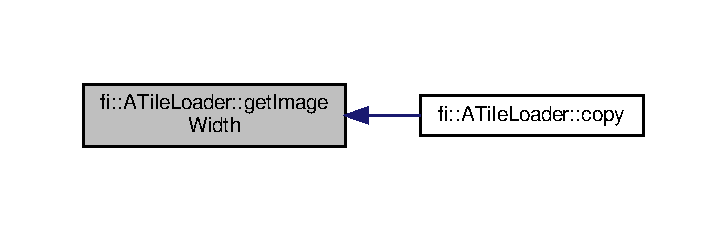
\includegraphics[width=349pt]{dc/d54/classfi_1_1ATileLoader_ad775bcbdddf7da6bb3f857a53c075a86_icgraph}
\end{center}
\end{figure}
\mbox{\Hypertarget{classfi_1_1ATileLoader_abb4cad235d57fbfb29ff5d37caf32a62}\label{classfi_1_1ATileLoader_abb4cad235d57fbfb29ff5d37caf32a62}} 
\index{fi\+::\+A\+Tile\+Loader@{fi\+::\+A\+Tile\+Loader}!get\+Name@{get\+Name}}
\index{get\+Name@{get\+Name}!fi\+::\+A\+Tile\+Loader@{fi\+::\+A\+Tile\+Loader}}
\subsubsection{\texorpdfstring{get\+Name()}{getName()}}
{\footnotesize\ttfamily template$<$typename User\+Type$>$ \\
std\+::string \hyperlink{classfi_1_1ATileLoader}{fi\+::\+A\+Tile\+Loader}$<$ User\+Type $>$\+::get\+Name (\begin{DoxyParamCaption}{ }\end{DoxyParamCaption})\hspace{0.3cm}{\ttfamily [override]}, {\ttfamily [pure virtual]}}



Get task name. 

\begin{DoxyReturn}{Returns}
Task name 
\end{DoxyReturn}


Implemented in \hyperlink{classfi_1_1GrayscaleTiffTileLoader_a66be68fc0c11aefbcb141ddb8c9e4deb}{fi\+::\+Grayscale\+Tiff\+Tile\+Loader$<$ User\+Type $>$}.

Here is the caller graph for this function\+:
\nopagebreak
\begin{figure}[H]
\begin{center}
\leavevmode
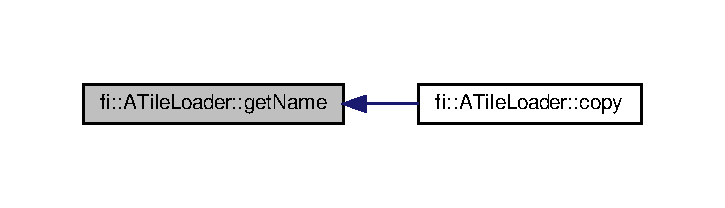
\includegraphics[width=348pt]{dc/d54/classfi_1_1ATileLoader_abb4cad235d57fbfb29ff5d37caf32a62_icgraph}
\end{center}
\end{figure}
\mbox{\Hypertarget{classfi_1_1ATileLoader_ad6550495be22454b5f72d46c68622c37}\label{classfi_1_1ATileLoader_ad6550495be22454b5f72d46c68622c37}} 
\index{fi\+::\+A\+Tile\+Loader@{fi\+::\+A\+Tile\+Loader}!get\+Nb\+Pyramid\+Levels@{get\+Nb\+Pyramid\+Levels}}
\index{get\+Nb\+Pyramid\+Levels@{get\+Nb\+Pyramid\+Levels}!fi\+::\+A\+Tile\+Loader@{fi\+::\+A\+Tile\+Loader}}
\subsubsection{\texorpdfstring{get\+Nb\+Pyramid\+Levels()}{getNbPyramidLevels()}}
{\footnotesize\ttfamily template$<$typename User\+Type$>$ \\
virtual uint32\+\_\+t \hyperlink{classfi_1_1ATileLoader}{fi\+::\+A\+Tile\+Loader}$<$ User\+Type $>$\+::get\+Nb\+Pyramid\+Levels (\begin{DoxyParamCaption}{ }\end{DoxyParamCaption}) const\hspace{0.3cm}{\ttfamily [pure virtual]}}



Get number of pyramid levels. 

\begin{DoxyReturn}{Returns}
Number of Pyramid levels 
\end{DoxyReturn}


Implemented in \hyperlink{classfi_1_1GrayscaleTiffTileLoader_a3a915d36a8c88a687b04ee8d5a15ecb0}{fi\+::\+Grayscale\+Tiff\+Tile\+Loader$<$ User\+Type $>$}.

Here is the caller graph for this function\+:
\nopagebreak
\begin{figure}[H]
\begin{center}
\leavevmode
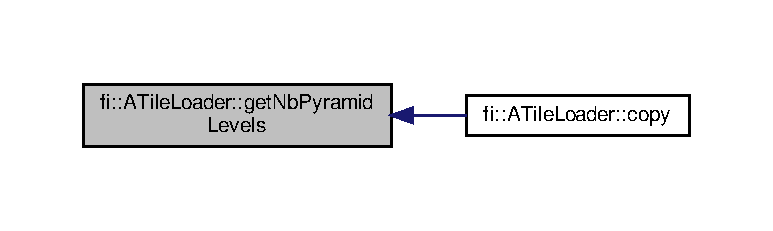
\includegraphics[width=350pt]{dc/d54/classfi_1_1ATileLoader_ad6550495be22454b5f72d46c68622c37_icgraph}
\end{center}
\end{figure}
\mbox{\Hypertarget{classfi_1_1ATileLoader_a531ceb7c73457fdde7055e95abd777fa}\label{classfi_1_1ATileLoader_a531ceb7c73457fdde7055e95abd777fa}} 
\index{fi\+::\+A\+Tile\+Loader@{fi\+::\+A\+Tile\+Loader}!get\+Tile\+Height@{get\+Tile\+Height}}
\index{get\+Tile\+Height@{get\+Tile\+Height}!fi\+::\+A\+Tile\+Loader@{fi\+::\+A\+Tile\+Loader}}
\subsubsection{\texorpdfstring{get\+Tile\+Height()}{getTileHeight()}}
{\footnotesize\ttfamily template$<$typename User\+Type$>$ \\
virtual uint32\+\_\+t \hyperlink{classfi_1_1ATileLoader}{fi\+::\+A\+Tile\+Loader}$<$ User\+Type $>$\+::get\+Tile\+Height (\begin{DoxyParamCaption}\item[{uint32\+\_\+t}]{level = {\ttfamily 0} }\end{DoxyParamCaption}) const\hspace{0.3cm}{\ttfamily [pure virtual]}}



Getter to tile Height. 

\begin{DoxyReturn}{Returns}
Tile Height 
\end{DoxyReturn}


Implemented in \hyperlink{classfi_1_1GrayscaleTiffTileLoader_aa1ac88ed6b9505d5c98b9202e6f1ee6d}{fi\+::\+Grayscale\+Tiff\+Tile\+Loader$<$ User\+Type $>$}.

Here is the caller graph for this function\+:
\nopagebreak
\begin{figure}[H]
\begin{center}
\leavevmode
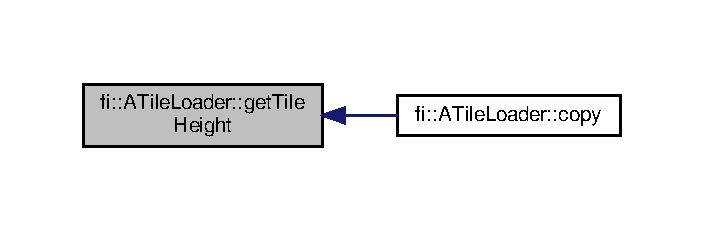
\includegraphics[width=338pt]{dc/d54/classfi_1_1ATileLoader_a531ceb7c73457fdde7055e95abd777fa_icgraph}
\end{center}
\end{figure}
\mbox{\Hypertarget{classfi_1_1ATileLoader_ad4ced663628b4134fd8f7bb0cfd2a652}\label{classfi_1_1ATileLoader_ad4ced663628b4134fd8f7bb0cfd2a652}} 
\index{fi\+::\+A\+Tile\+Loader@{fi\+::\+A\+Tile\+Loader}!get\+Tile\+Width@{get\+Tile\+Width}}
\index{get\+Tile\+Width@{get\+Tile\+Width}!fi\+::\+A\+Tile\+Loader@{fi\+::\+A\+Tile\+Loader}}
\subsubsection{\texorpdfstring{get\+Tile\+Width()}{getTileWidth()}}
{\footnotesize\ttfamily template$<$typename User\+Type$>$ \\
virtual uint32\+\_\+t \hyperlink{classfi_1_1ATileLoader}{fi\+::\+A\+Tile\+Loader}$<$ User\+Type $>$\+::get\+Tile\+Width (\begin{DoxyParamCaption}\item[{uint32\+\_\+t}]{level = {\ttfamily 0} }\end{DoxyParamCaption}) const\hspace{0.3cm}{\ttfamily [pure virtual]}}



Getter to tile Width. 

\begin{DoxyReturn}{Returns}
Tile Width 
\end{DoxyReturn}


Implemented in \hyperlink{classfi_1_1GrayscaleTiffTileLoader_a273613b0ebb48732c449399fac614ebd}{fi\+::\+Grayscale\+Tiff\+Tile\+Loader$<$ User\+Type $>$}.

Here is the caller graph for this function\+:
\nopagebreak
\begin{figure}[H]
\begin{center}
\leavevmode
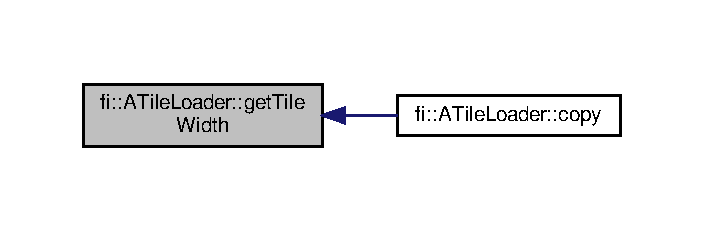
\includegraphics[width=338pt]{dc/d54/classfi_1_1ATileLoader_ad4ced663628b4134fd8f7bb0cfd2a652_icgraph}
\end{center}
\end{figure}
\mbox{\Hypertarget{classfi_1_1ATileLoader_a12929a1a82ff9cf2615e7a7420ba92c4}\label{classfi_1_1ATileLoader_a12929a1a82ff9cf2615e7a7420ba92c4}} 
\index{fi\+::\+A\+Tile\+Loader@{fi\+::\+A\+Tile\+Loader}!initialize@{initialize}}
\index{initialize@{initialize}!fi\+::\+A\+Tile\+Loader@{fi\+::\+A\+Tile\+Loader}}
\subsubsection{\texorpdfstring{initialize()}{initialize()}}
{\footnotesize\ttfamily template$<$typename User\+Type$>$ \\
void \hyperlink{classfi_1_1ATileLoader}{fi\+::\+A\+Tile\+Loader}$<$ User\+Type $>$\+::initialize (\begin{DoxyParamCaption}{ }\end{DoxyParamCaption})\hspace{0.3cm}{\ttfamily [inline]}, {\ttfamily [final]}}



Initialize function. 

Associate a cache from the pool to a specific tile loader 

Definition at line 94 of file A\+Tile\+Loader.\+h.

Here is the call graph for this function\+:
\nopagebreak
\begin{figure}[H]
\begin{center}
\leavevmode
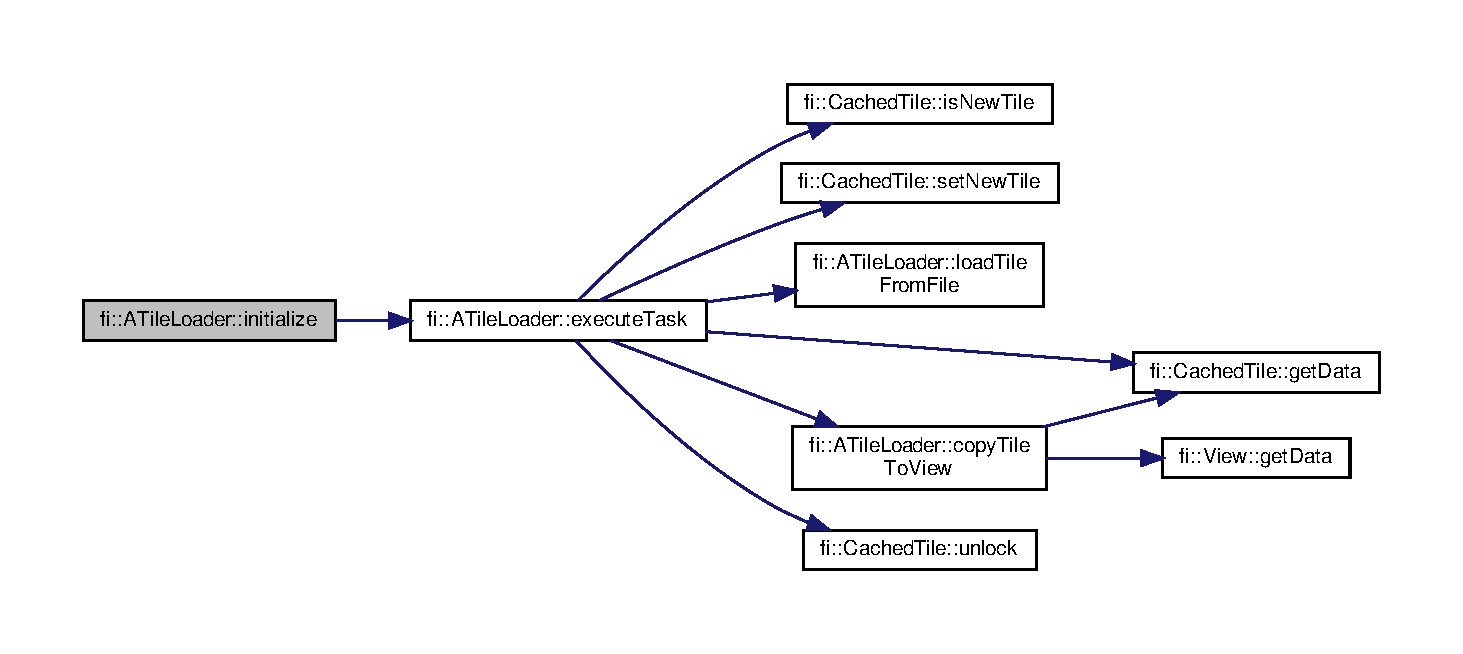
\includegraphics[width=350pt]{dc/d54/classfi_1_1ATileLoader_a12929a1a82ff9cf2615e7a7420ba92c4_cgraph}
\end{center}
\end{figure}
\mbox{\Hypertarget{classfi_1_1ATileLoader_a46d85c52fe89339a3ffbc1cb9c377eb0}\label{classfi_1_1ATileLoader_a46d85c52fe89339a3ffbc1cb9c377eb0}} 
\index{fi\+::\+A\+Tile\+Loader@{fi\+::\+A\+Tile\+Loader}!load\+Tile\+From\+File@{load\+Tile\+From\+File}}
\index{load\+Tile\+From\+File@{load\+Tile\+From\+File}!fi\+::\+A\+Tile\+Loader@{fi\+::\+A\+Tile\+Loader}}
\subsubsection{\texorpdfstring{load\+Tile\+From\+File()}{loadTileFromFile()}}
{\footnotesize\ttfamily template$<$typename User\+Type$>$ \\
virtual double \hyperlink{classfi_1_1ATileLoader}{fi\+::\+A\+Tile\+Loader}$<$ User\+Type $>$\+::load\+Tile\+From\+File (\begin{DoxyParamCaption}\item[{User\+Type $\ast$}]{tile,  }\item[{uint32\+\_\+t}]{index\+Row\+Global\+Tile,  }\item[{uint32\+\_\+t}]{index\+Col\+Global\+Tile }\end{DoxyParamCaption})\hspace{0.3cm}{\ttfamily [pure virtual]}}



Load a specific Tile at 0 based indexes (index\+Row\+Global\+Tile, index\+Col\+Global\+Tile) of size tile\+Height x tile\+Width. 


\begin{DoxyParams}{Parameters}
{\em tile} & to load into \\
\hline
{\em index\+Row\+Global\+Tile} & Tile row index \\
\hline
{\em index\+Col\+Global\+Tile} & Tile col index \\
\hline
\end{DoxyParams}
\begin{DoxyReturn}{Returns}
Duration in mS to load a tile from the disk, use for statistics purpose 
\end{DoxyReturn}


Implemented in \hyperlink{classfi_1_1GrayscaleTiffTileLoader_af52ec5177c51882b9544ee9684f7a2ae}{fi\+::\+Grayscale\+Tiff\+Tile\+Loader$<$ User\+Type $>$}.

Here is the caller graph for this function\+:
\nopagebreak
\begin{figure}[H]
\begin{center}
\leavevmode
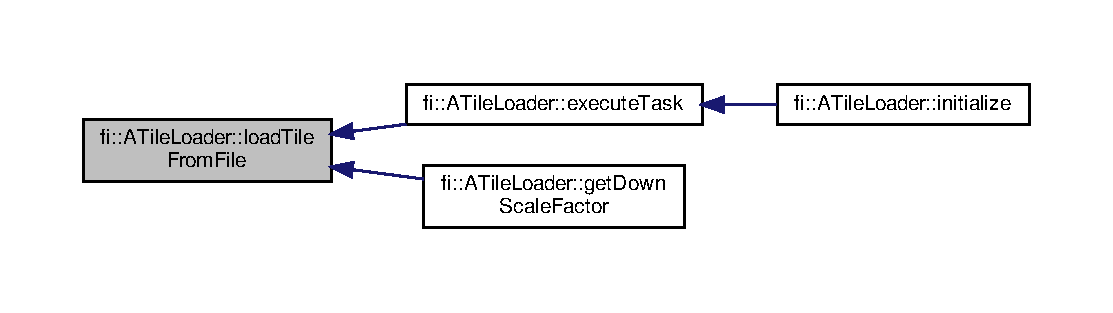
\includegraphics[width=350pt]{dc/d54/classfi_1_1ATileLoader_a46d85c52fe89339a3ffbc1cb9c377eb0_icgraph}
\end{center}
\end{figure}
\mbox{\Hypertarget{classfi_1_1ATileLoader_a1113a06fc88a278bede14bbee2ae4a59}\label{classfi_1_1ATileLoader_a1113a06fc88a278bede14bbee2ae4a59}} 
\index{fi\+::\+A\+Tile\+Loader@{fi\+::\+A\+Tile\+Loader}!set\+Cache@{set\+Cache}}
\index{set\+Cache@{set\+Cache}!fi\+::\+A\+Tile\+Loader@{fi\+::\+A\+Tile\+Loader}}
\subsubsection{\texorpdfstring{set\+Cache()}{setCache()}}
{\footnotesize\ttfamily template$<$typename User\+Type$>$ \\
void \hyperlink{classfi_1_1ATileLoader}{fi\+::\+A\+Tile\+Loader}$<$ User\+Type $>$\+::set\+Cache (\begin{DoxyParamCaption}\item[{std\+::vector$<$ \hyperlink{classfi_1_1FigCache}{fi\+::\+Fig\+Cache}$<$ User\+Type $>$ $\ast$$>$ \&}]{all\+Cache }\end{DoxyParamCaption})\hspace{0.3cm}{\ttfamily [inline]}}



Set the caches. 


\begin{DoxyParams}{Parameters}
{\em all\+Cache} & Caches to set \\
\hline
\end{DoxyParams}


Definition at line 158 of file A\+Tile\+Loader.\+h.



\subsection{Member Data Documentation}
\mbox{\Hypertarget{classfi_1_1ATileLoader_a07679e26c08c1f998e00cdf3e1af5d43}\label{classfi_1_1ATileLoader_a07679e26c08c1f998e00cdf3e1af5d43}} 
\index{fi\+::\+A\+Tile\+Loader@{fi\+::\+A\+Tile\+Loader}!\+\_\+all\+Cache@{\+\_\+all\+Cache}}
\index{\+\_\+all\+Cache@{\+\_\+all\+Cache}!fi\+::\+A\+Tile\+Loader@{fi\+::\+A\+Tile\+Loader}}
\subsubsection{\texorpdfstring{\+\_\+all\+Cache}{\_allCache}}
{\footnotesize\ttfamily template$<$typename User\+Type$>$ \\
std\+::vector$<$\hyperlink{classfi_1_1FigCache}{fi\+::\+Fig\+Cache}$<$User\+Type$>$ $\ast$$>$ \hyperlink{classfi_1_1ATileLoader}{fi\+::\+A\+Tile\+Loader}$<$ User\+Type $>$\+::\+\_\+all\+Cache\hspace{0.3cm}{\ttfamily [private]}}



All caches for each pyramid levels. 



Definition at line 227 of file A\+Tile\+Loader.\+h.

\mbox{\Hypertarget{classfi_1_1ATileLoader_a35c8ba6cc53333935c03d822b24095b9}\label{classfi_1_1ATileLoader_a35c8ba6cc53333935c03d822b24095b9}} 
\index{fi\+::\+A\+Tile\+Loader@{fi\+::\+A\+Tile\+Loader}!\+\_\+cache@{\+\_\+cache}}
\index{\+\_\+cache@{\+\_\+cache}!fi\+::\+A\+Tile\+Loader@{fi\+::\+A\+Tile\+Loader}}
\subsubsection{\texorpdfstring{\+\_\+cache}{\_cache}}
{\footnotesize\ttfamily template$<$typename User\+Type$>$ \\
\hyperlink{classfi_1_1FigCache}{Fig\+Cache}$<$User\+Type$>$$\ast$ \hyperlink{classfi_1_1ATileLoader}{fi\+::\+A\+Tile\+Loader}$<$ User\+Type $>$\+::\+\_\+cache = nullptr\hspace{0.3cm}{\ttfamily [private]}}



Tile Cache. 



Definition at line 230 of file A\+Tile\+Loader.\+h.

\mbox{\Hypertarget{classfi_1_1ATileLoader_aa96fb4d90ac425c4b670b23f6ebe49f6}\label{classfi_1_1ATileLoader_aa96fb4d90ac425c4b670b23f6ebe49f6}} 
\index{fi\+::\+A\+Tile\+Loader@{fi\+::\+A\+Tile\+Loader}!\+\_\+file\+Path@{\+\_\+file\+Path}}
\index{\+\_\+file\+Path@{\+\_\+file\+Path}!fi\+::\+A\+Tile\+Loader@{fi\+::\+A\+Tile\+Loader}}
\subsubsection{\texorpdfstring{\+\_\+file\+Path}{\_filePath}}
{\footnotesize\ttfamily template$<$typename User\+Type$>$ \\
std\+::string \hyperlink{classfi_1_1ATileLoader}{fi\+::\+A\+Tile\+Loader}$<$ User\+Type $>$\+::\+\_\+file\+Path\hspace{0.3cm}{\ttfamily [protected]}}



Path to file to load. 



Definition at line 223 of file A\+Tile\+Loader.\+h.



The documentation for this class was generated from the following file\+:\begin{DoxyCompactItemize}
\item 
/home/anb22/\+Documents/\+Fast-\/\+Image/\+Fast\+Image/src/\+Fast\+Image/api/\hyperlink{ATileLoader_8h}{A\+Tile\+Loader.\+h}\end{DoxyCompactItemize}

\hypertarget{classfc_1_1Blob}{}\section{fc\+:\+:Blob Class Reference}
\label{classfc_1_1Blob}\index{fc\+::\+Blob@{fc\+::\+Blob}}


\hyperlink{classfc_1_1Blob}{Blob} representing a part of a feature.  




{\ttfamily \#include $<$Fast\+Image/\+Feature\+Collection/\+Data/\+Blob.\+h$>$}



Collaboration diagram for fc\+:\+:Blob\+:
\nopagebreak
\begin{figure}[H]
\begin{center}
\leavevmode
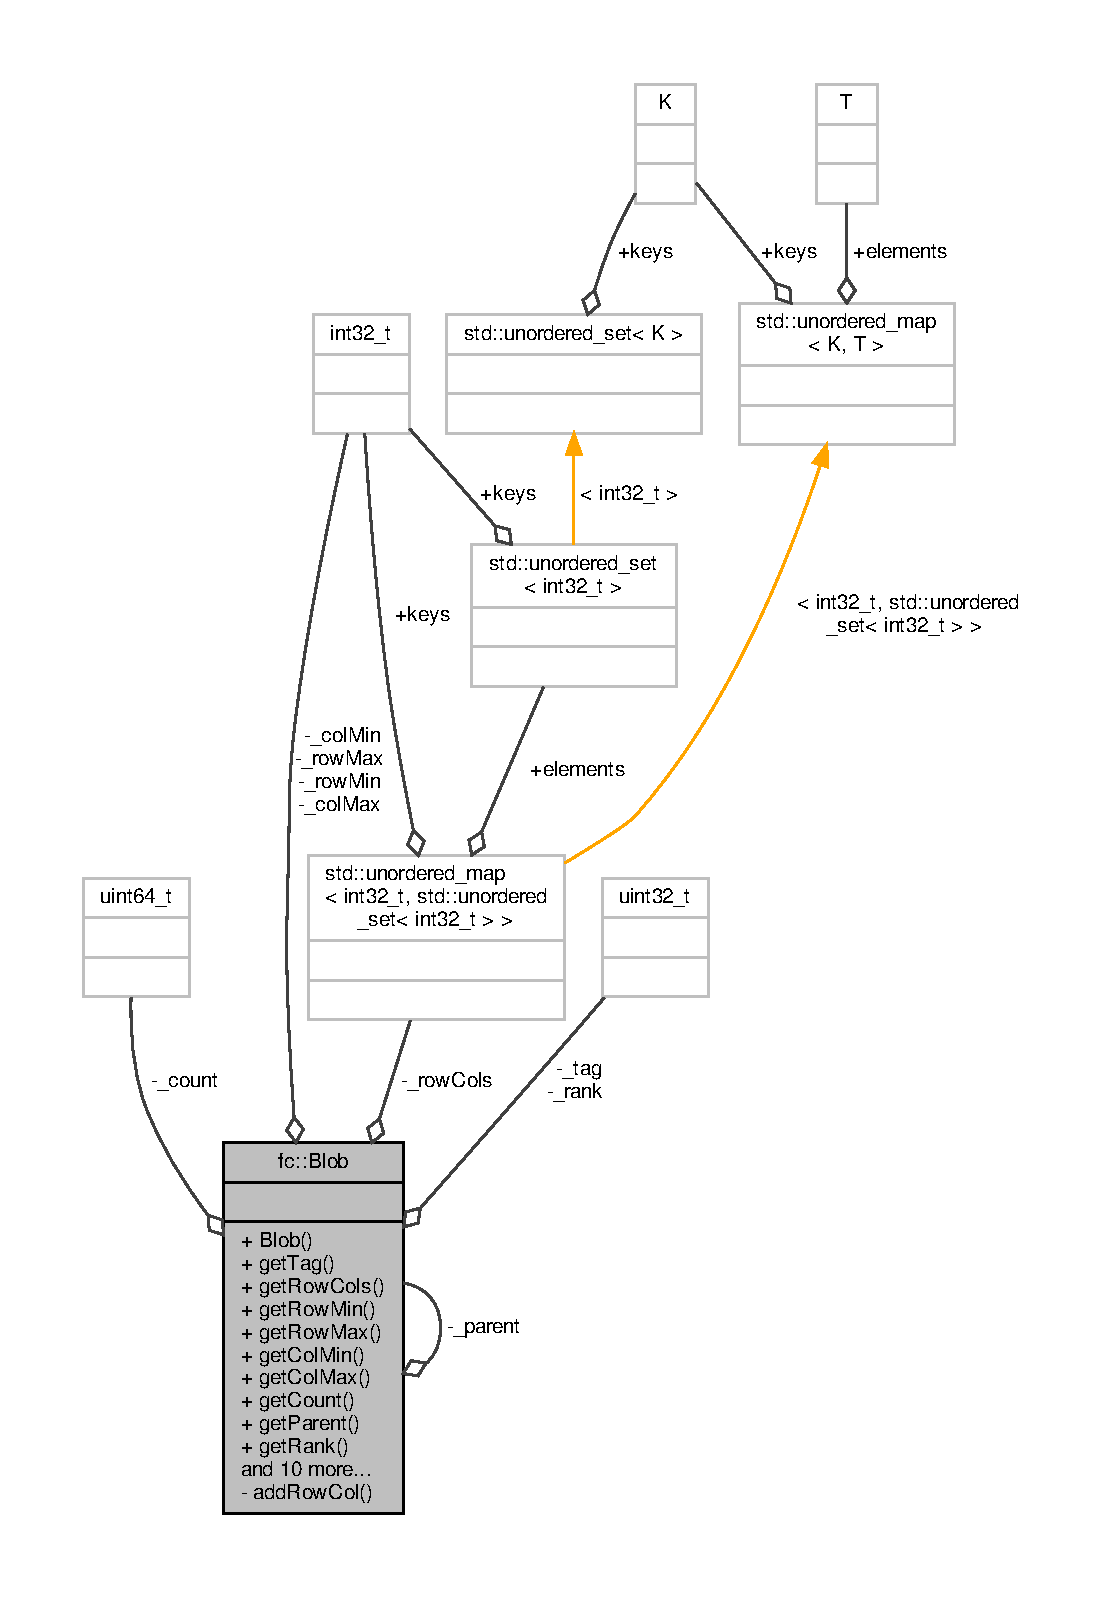
\includegraphics[width=350pt]{d9/d0a/classfc_1_1Blob__coll__graph}
\end{center}
\end{figure}
\subsection*{Public Member Functions}
\begin{DoxyCompactItemize}
\item 
\hyperlink{classfc_1_1Blob_ac52255b13f4ce401de0a4310d846c62a}{Blob} ()
\begin{DoxyCompactList}\small\item\em \hyperlink{classfc_1_1Blob}{Blob} construction and initialisation. \end{DoxyCompactList}\item 
uint32\+\_\+t \hyperlink{classfc_1_1Blob_aeb84112e584a5e918530690b42cfd8f6}{get\+Tag} () const
\begin{DoxyCompactList}\small\item\em Get \hyperlink{classfc_1_1Blob}{Blob} tag. \end{DoxyCompactList}\item 
std\+::unordered\+\_\+map$<$ int32\+\_\+t, std\+::unordered\+\_\+set$<$ int32\+\_\+t $>$ $>$ \& \hyperlink{classfc_1_1Blob_a80e63b761ebffdf90dea47b8a59b2c32}{get\+Row\+Cols} ()
\begin{DoxyCompactList}\small\item\em Get sparse matrix structure. \end{DoxyCompactList}\item 
int32\+\_\+t \hyperlink{classfc_1_1Blob_a167b6c3a33f301a7dcb527b289dd0834}{get\+Row\+Min} () const
\begin{DoxyCompactList}\small\item\em Get minimum bounding box row. \end{DoxyCompactList}\item 
int32\+\_\+t \hyperlink{classfc_1_1Blob_af4a030b9ba08fd02242137a296a3692b}{get\+Row\+Max} () const
\begin{DoxyCompactList}\small\item\em Get maximum bounding box row. \end{DoxyCompactList}\item 
int32\+\_\+t \hyperlink{classfc_1_1Blob_ac4e8548eb6f47c1febbd70184bee315a}{get\+Col\+Min} () const
\begin{DoxyCompactList}\small\item\em Get minimum bounding box col. \end{DoxyCompactList}\item 
int32\+\_\+t \hyperlink{classfc_1_1Blob_a1f9cfacc7e5d2f048c26f8b9c706141a}{get\+Col\+Max} () const
\begin{DoxyCompactList}\small\item\em Get maximum bounding box col. \end{DoxyCompactList}\item 
uint64\+\_\+t \hyperlink{classfc_1_1Blob_a7443f8362ad88c61e5dcfae2dad54d47}{get\+Count} () const
\begin{DoxyCompactList}\small\item\em Get number of pixels in a blob. \end{DoxyCompactList}\item 
\hyperlink{classfc_1_1Blob}{Blob} $\ast$ \hyperlink{classfc_1_1Blob_afde20e8b149cc08b56bac810177c4836}{get\+Parent} () const
\begin{DoxyCompactList}\small\item\em Get blob parent, used by Union find. \end{DoxyCompactList}\item 
uint32\+\_\+t \hyperlink{classfc_1_1Blob_a368c9607fb6d7e032795d742eaed1539}{get\+Rank} () const
\begin{DoxyCompactList}\small\item\em Get blob rank, used by Union find. \end{DoxyCompactList}\item 
bool \hyperlink{classfc_1_1Blob_a462ba30be4256cccc0270ab0d278bb07}{is\+Pixelin\+Feature} (int32\+\_\+t row, int32\+\_\+t col)
\begin{DoxyCompactList}\small\item\em Test if a pixel is in a blob. \end{DoxyCompactList}\item 
void \hyperlink{classfc_1_1Blob_a14a42d0f0fe5a8c06444609027faecbe}{set\+Row\+Min} (int32\+\_\+t row\+Min)
\begin{DoxyCompactList}\small\item\em Minimum bounding box row setter. \end{DoxyCompactList}\item 
void \hyperlink{classfc_1_1Blob_af726d6434723c76d5c9e793a99a01408}{set\+Row\+Max} (int32\+\_\+t row\+Max)
\begin{DoxyCompactList}\small\item\em Maximum bounding box row setter. \end{DoxyCompactList}\item 
void \hyperlink{classfc_1_1Blob_aa9972e1dd32aa399426b87bc4c610d69}{set\+Col\+Min} (int32\+\_\+t col\+Min)
\begin{DoxyCompactList}\small\item\em Minimum bounding box col setter. \end{DoxyCompactList}\item 
void \hyperlink{classfc_1_1Blob_a0534b6d033d5dc27f24f7f7776b148c0}{set\+Col\+Max} (int32\+\_\+t col\+Max)
\begin{DoxyCompactList}\small\item\em Maximum bounding box col setter. \end{DoxyCompactList}\item 
void \hyperlink{classfc_1_1Blob_a4f404eafaf95bd017eecfbd234eb650e}{set\+Count} (uint64\+\_\+t count)
\begin{DoxyCompactList}\small\item\em Count setter. \end{DoxyCompactList}\item 
void \hyperlink{classfc_1_1Blob_a88b9a5ef4d1ea26fd9e313b8d033d721}{set\+Parent} (\hyperlink{classfc_1_1Blob}{Blob} $\ast$parent)
\begin{DoxyCompactList}\small\item\em \hyperlink{classfc_1_1Blob}{Blob} parent setter Used by Union find algorithm. \end{DoxyCompactList}\item 
void \hyperlink{classfc_1_1Blob_a21fdbcaf66775d27bb7680402fe2fd8a}{set\+Rank} (uint32\+\_\+t rank)
\begin{DoxyCompactList}\small\item\em \hyperlink{classfc_1_1Blob}{Blob} rank setter Used by Union find algorithm. \end{DoxyCompactList}\item 
void \hyperlink{classfc_1_1Blob_a01be7313665ad198c73220165a008f2b}{add\+Pixel} (int32\+\_\+t row, int32\+\_\+t col)
\begin{DoxyCompactList}\small\item\em Add a pixel to the blob and update blob metadata. \end{DoxyCompactList}\item 
\hyperlink{classfc_1_1Blob}{Blob} $\ast$ \hyperlink{classfc_1_1Blob_ae84692d9e132dd046b56bb6ac06dd8bb}{merge\+And\+Delete} (\hyperlink{classfc_1_1Blob}{Blob} $\ast$blob)
\begin{DoxyCompactList}\small\item\em Merge 2 blobs, and delete the unused one. \end{DoxyCompactList}\end{DoxyCompactItemize}
\subsection*{Private Member Functions}
\begin{DoxyCompactItemize}
\item 
void \hyperlink{classfc_1_1Blob_a4c9d015ad9326b4f5688af7ae190e613}{add\+Row\+Col} (int32\+\_\+t row, int32\+\_\+t col)
\begin{DoxyCompactList}\small\item\em Add a pixel to the sparse matrix. \end{DoxyCompactList}\end{DoxyCompactItemize}
\subsection*{Private Attributes}
\begin{DoxyCompactItemize}
\item 
\hyperlink{classfc_1_1Blob}{Blob} $\ast$ \hyperlink{classfc_1_1Blob_ab58442d32a4ce2e9d5c4718d63e126d8}{\+\_\+parent} = nullptr
\begin{DoxyCompactList}\small\item\em \hyperlink{classfc_1_1Blob}{Blob} parent, used by the Union find algorithm. \end{DoxyCompactList}\item 
uint32\+\_\+t \hyperlink{classfc_1_1Blob_ad19347abbefa18b6e98e1156cf09fe3a}{\+\_\+rank} = 0
\begin{DoxyCompactList}\small\item\em \hyperlink{classfc_1_1Blob}{Blob} rank, used by the Union find algorithm. \end{DoxyCompactList}\item 
uint32\+\_\+t \hyperlink{classfc_1_1Blob_af07e1270217289a0879386f267bf5fe5}{\+\_\+tag} = 0
\begin{DoxyCompactList}\small\item\em Tag, only used to print/debug purpose. \end{DoxyCompactList}\item 
int32\+\_\+t \hyperlink{classfc_1_1Blob_ab63888a3d59cb3b81ad10e19864b101a}{\+\_\+row\+Min} \{\}
\begin{DoxyCompactList}\small\item\em Minimum bounding box row. \end{DoxyCompactList}\item 
int32\+\_\+t \hyperlink{classfc_1_1Blob_ada6057ee4bf33c0a432f28d5d42413dd}{\+\_\+row\+Max} \{\}
\begin{DoxyCompactList}\small\item\em Maximum bounding box row. \end{DoxyCompactList}\item 
int32\+\_\+t \hyperlink{classfc_1_1Blob_aa962a217328b361385584042e8d29eb9}{\+\_\+col\+Min} \{\}
\begin{DoxyCompactList}\small\item\em Minimum bounding box col. \end{DoxyCompactList}\item 
int32\+\_\+t \hyperlink{classfc_1_1Blob_ab35bcad8687bcbd04b0a7952702a88a6}{\+\_\+col\+Max} \{\}
\begin{DoxyCompactList}\small\item\em Maximum bounding box col. \end{DoxyCompactList}\item 
uint64\+\_\+t \hyperlink{classfc_1_1Blob_a7a36fdbf8d1c967b0664613f1b7f3a98}{\+\_\+count} \{\}
\begin{DoxyCompactList}\small\item\em Number of pixel to fastened the blob merge. \end{DoxyCompactList}\item 
std\+::unordered\+\_\+map$<$ int32\+\_\+t, std\+::unordered\+\_\+set$<$ int32\+\_\+t $>$ $>$ \hyperlink{classfc_1_1Blob_a2688a4b64b2e3d37e7309aca03177b55}{\+\_\+row\+Cols} \{\}
\begin{DoxyCompactList}\small\item\em Sparse matrix of unique coordinates composing the blob. \end{DoxyCompactList}\end{DoxyCompactItemize}
\subsection*{Friends}
\begin{DoxyCompactItemize}
\item 
std\+::ostream \& \hyperlink{classfc_1_1Blob_a5fe38c43bc6a7886e8760e7b00ade43a}{operator$<$$<$} (std\+::ostream \&os, const \hyperlink{classfc_1_1Blob}{Blob} \&blob)
\begin{DoxyCompactList}\small\item\em Print blob state. \end{DoxyCompactList}\end{DoxyCompactItemize}


\subsection{Detailed Description}
\hyperlink{classfc_1_1Blob}{Blob} representing a part of a feature. 

It is composed by a bounding box from the point (row\+Min, row\+Max) to (row\+M\+Ax, Col\+Max).The bounding box delimit a sparse matrix representing the pixels part of this blob. A blob has a specific id, called tag. 

Definition at line 65 of file Blob.\+h.



\subsection{Constructor \& Destructor Documentation}
\mbox{\Hypertarget{classfc_1_1Blob_ac52255b13f4ce401de0a4310d846c62a}\label{classfc_1_1Blob_ac52255b13f4ce401de0a4310d846c62a}} 
\index{fc\+::\+Blob@{fc\+::\+Blob}!Blob@{Blob}}
\index{Blob@{Blob}!fc\+::\+Blob@{fc\+::\+Blob}}
\subsubsection{\texorpdfstring{Blob()}{Blob()}}
{\footnotesize\ttfamily fc\+::\+Blob\+::\+Blob (\begin{DoxyParamCaption}{ }\end{DoxyParamCaption})\hspace{0.3cm}{\ttfamily [inline]}}



\hyperlink{classfc_1_1Blob}{Blob} construction and initialisation. 



Definition at line 68 of file Blob.\+h.



\subsection{Member Function Documentation}
\mbox{\Hypertarget{classfc_1_1Blob_a01be7313665ad198c73220165a008f2b}\label{classfc_1_1Blob_a01be7313665ad198c73220165a008f2b}} 
\index{fc\+::\+Blob@{fc\+::\+Blob}!add\+Pixel@{add\+Pixel}}
\index{add\+Pixel@{add\+Pixel}!fc\+::\+Blob@{fc\+::\+Blob}}
\subsubsection{\texorpdfstring{add\+Pixel()}{addPixel()}}
{\footnotesize\ttfamily void fc\+::\+Blob\+::add\+Pixel (\begin{DoxyParamCaption}\item[{int32\+\_\+t}]{row,  }\item[{int32\+\_\+t}]{col }\end{DoxyParamCaption})\hspace{0.3cm}{\ttfamily [inline]}}



Add a pixel to the blob and update blob metadata. 


\begin{DoxyParams}{Parameters}
{\em row} & Pixel\textquotesingle{}s row \\
\hline
{\em col} & Pixel\textquotesingle{}s col \\
\hline
\end{DoxyParams}


Definition at line 170 of file Blob.\+h.

Here is the call graph for this function\+:
\nopagebreak
\begin{figure}[H]
\begin{center}
\leavevmode
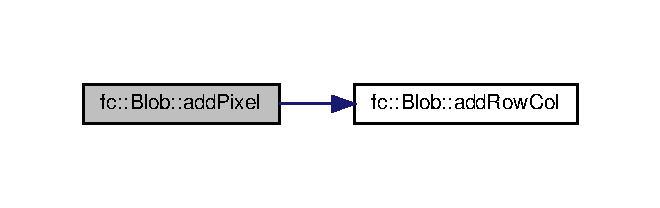
\includegraphics[width=317pt]{d2/d7e/classfc_1_1Blob_a01be7313665ad198c73220165a008f2b_cgraph}
\end{center}
\end{figure}
Here is the caller graph for this function\+:
\nopagebreak
\begin{figure}[H]
\begin{center}
\leavevmode
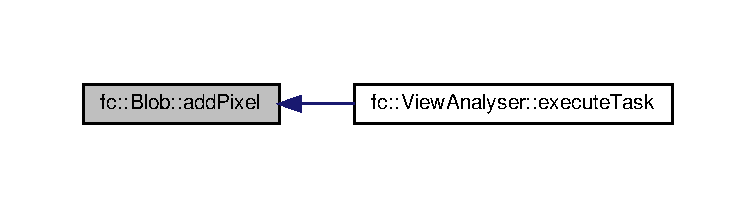
\includegraphics[width=350pt]{d2/d7e/classfc_1_1Blob_a01be7313665ad198c73220165a008f2b_icgraph}
\end{center}
\end{figure}
\mbox{\Hypertarget{classfc_1_1Blob_a4c9d015ad9326b4f5688af7ae190e613}\label{classfc_1_1Blob_a4c9d015ad9326b4f5688af7ae190e613}} 
\index{fc\+::\+Blob@{fc\+::\+Blob}!add\+Row\+Col@{add\+Row\+Col}}
\index{add\+Row\+Col@{add\+Row\+Col}!fc\+::\+Blob@{fc\+::\+Blob}}
\subsubsection{\texorpdfstring{add\+Row\+Col()}{addRowCol()}}
{\footnotesize\ttfamily void fc\+::\+Blob\+::add\+Row\+Col (\begin{DoxyParamCaption}\item[{int32\+\_\+t}]{row,  }\item[{int32\+\_\+t}]{col }\end{DoxyParamCaption})\hspace{0.3cm}{\ttfamily [inline]}, {\ttfamily [private]}}



Add a pixel to the sparse matrix. 


\begin{DoxyParams}{Parameters}
{\em row} & Pixel row \\
\hline
{\em col} & Pixel col \\
\hline
\end{DoxyParams}


Definition at line 243 of file Blob.\+h.

Here is the caller graph for this function\+:
\nopagebreak
\begin{figure}[H]
\begin{center}
\leavevmode
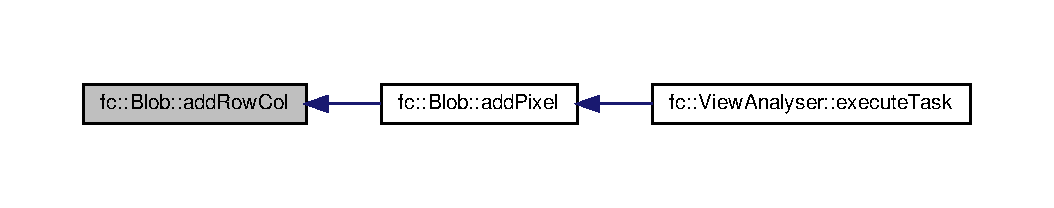
\includegraphics[width=350pt]{d2/d7e/classfc_1_1Blob_a4c9d015ad9326b4f5688af7ae190e613_icgraph}
\end{center}
\end{figure}
\mbox{\Hypertarget{classfc_1_1Blob_a1f9cfacc7e5d2f048c26f8b9c706141a}\label{classfc_1_1Blob_a1f9cfacc7e5d2f048c26f8b9c706141a}} 
\index{fc\+::\+Blob@{fc\+::\+Blob}!get\+Col\+Max@{get\+Col\+Max}}
\index{get\+Col\+Max@{get\+Col\+Max}!fc\+::\+Blob@{fc\+::\+Blob}}
\subsubsection{\texorpdfstring{get\+Col\+Max()}{getColMax()}}
{\footnotesize\ttfamily int32\+\_\+t fc\+::\+Blob\+::get\+Col\+Max (\begin{DoxyParamCaption}{ }\end{DoxyParamCaption}) const\hspace{0.3cm}{\ttfamily [inline]}}



Get maximum bounding box col. 

\begin{DoxyReturn}{Returns}
Maximum bounding box col 
\end{DoxyReturn}


Definition at line 110 of file Blob.\+h.

Here is the caller graph for this function\+:
\nopagebreak
\begin{figure}[H]
\begin{center}
\leavevmode
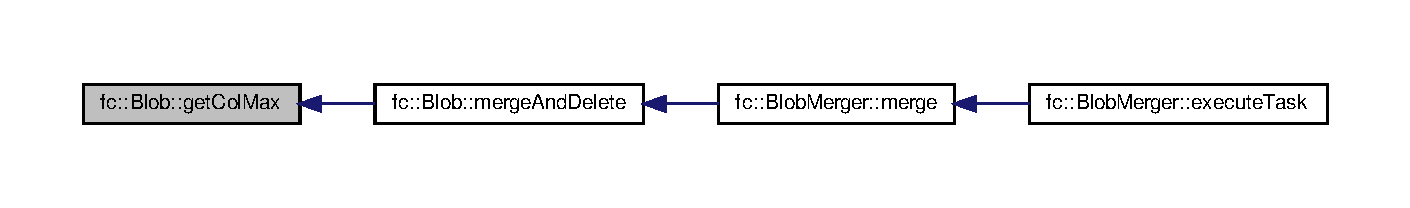
\includegraphics[width=350pt]{d2/d7e/classfc_1_1Blob_a1f9cfacc7e5d2f048c26f8b9c706141a_icgraph}
\end{center}
\end{figure}
\mbox{\Hypertarget{classfc_1_1Blob_ac4e8548eb6f47c1febbd70184bee315a}\label{classfc_1_1Blob_ac4e8548eb6f47c1febbd70184bee315a}} 
\index{fc\+::\+Blob@{fc\+::\+Blob}!get\+Col\+Min@{get\+Col\+Min}}
\index{get\+Col\+Min@{get\+Col\+Min}!fc\+::\+Blob@{fc\+::\+Blob}}
\subsubsection{\texorpdfstring{get\+Col\+Min()}{getColMin()}}
{\footnotesize\ttfamily int32\+\_\+t fc\+::\+Blob\+::get\+Col\+Min (\begin{DoxyParamCaption}{ }\end{DoxyParamCaption}) const\hspace{0.3cm}{\ttfamily [inline]}}



Get minimum bounding box col. 

\begin{DoxyReturn}{Returns}
Minimum bounding box col 
\end{DoxyReturn}


Definition at line 106 of file Blob.\+h.

Here is the caller graph for this function\+:
\nopagebreak
\begin{figure}[H]
\begin{center}
\leavevmode
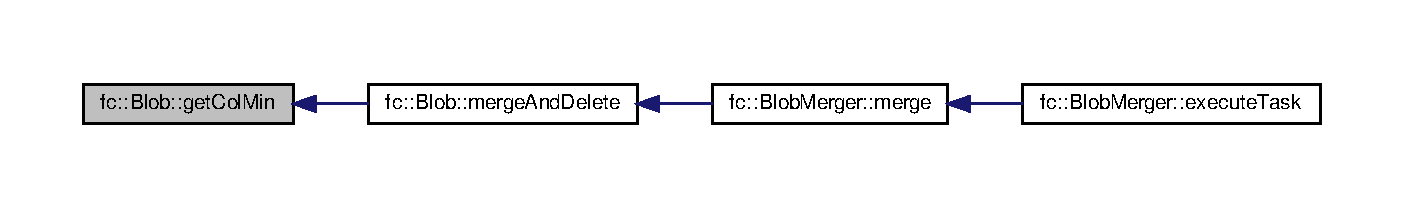
\includegraphics[width=350pt]{d2/d7e/classfc_1_1Blob_ac4e8548eb6f47c1febbd70184bee315a_icgraph}
\end{center}
\end{figure}
\mbox{\Hypertarget{classfc_1_1Blob_a7443f8362ad88c61e5dcfae2dad54d47}\label{classfc_1_1Blob_a7443f8362ad88c61e5dcfae2dad54d47}} 
\index{fc\+::\+Blob@{fc\+::\+Blob}!get\+Count@{get\+Count}}
\index{get\+Count@{get\+Count}!fc\+::\+Blob@{fc\+::\+Blob}}
\subsubsection{\texorpdfstring{get\+Count()}{getCount()}}
{\footnotesize\ttfamily uint64\+\_\+t fc\+::\+Blob\+::get\+Count (\begin{DoxyParamCaption}{ }\end{DoxyParamCaption}) const\hspace{0.3cm}{\ttfamily [inline]}}



Get number of pixels in a blob. 

\begin{DoxyReturn}{Returns}
Number of pixels in a blob 
\end{DoxyReturn}


Definition at line 114 of file Blob.\+h.

Here is the caller graph for this function\+:
\nopagebreak
\begin{figure}[H]
\begin{center}
\leavevmode
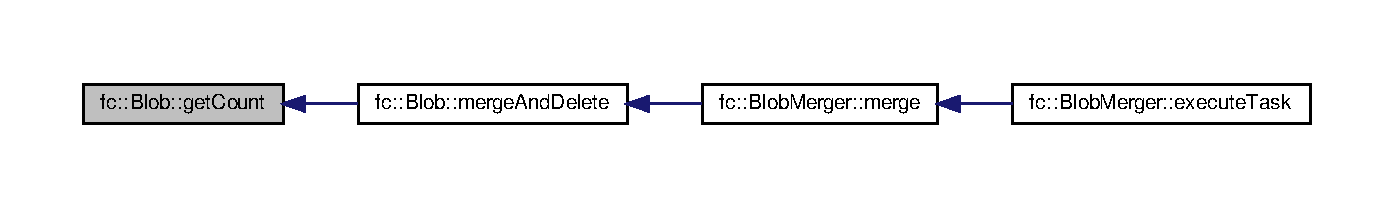
\includegraphics[width=350pt]{d2/d7e/classfc_1_1Blob_a7443f8362ad88c61e5dcfae2dad54d47_icgraph}
\end{center}
\end{figure}
\mbox{\Hypertarget{classfc_1_1Blob_afde20e8b149cc08b56bac810177c4836}\label{classfc_1_1Blob_afde20e8b149cc08b56bac810177c4836}} 
\index{fc\+::\+Blob@{fc\+::\+Blob}!get\+Parent@{get\+Parent}}
\index{get\+Parent@{get\+Parent}!fc\+::\+Blob@{fc\+::\+Blob}}
\subsubsection{\texorpdfstring{get\+Parent()}{getParent()}}
{\footnotesize\ttfamily \hyperlink{classfc_1_1Blob}{Blob}$\ast$ fc\+::\+Blob\+::get\+Parent (\begin{DoxyParamCaption}{ }\end{DoxyParamCaption}) const\hspace{0.3cm}{\ttfamily [inline]}}



Get blob parent, used by Union find. 

\begin{DoxyReturn}{Returns}
\hyperlink{classfc_1_1Blob}{Blob} parent 
\end{DoxyReturn}


Definition at line 118 of file Blob.\+h.

\mbox{\Hypertarget{classfc_1_1Blob_a368c9607fb6d7e032795d742eaed1539}\label{classfc_1_1Blob_a368c9607fb6d7e032795d742eaed1539}} 
\index{fc\+::\+Blob@{fc\+::\+Blob}!get\+Rank@{get\+Rank}}
\index{get\+Rank@{get\+Rank}!fc\+::\+Blob@{fc\+::\+Blob}}
\subsubsection{\texorpdfstring{get\+Rank()}{getRank()}}
{\footnotesize\ttfamily uint32\+\_\+t fc\+::\+Blob\+::get\+Rank (\begin{DoxyParamCaption}{ }\end{DoxyParamCaption}) const\hspace{0.3cm}{\ttfamily [inline]}}



Get blob rank, used by Union find. 

\begin{DoxyReturn}{Returns}
\hyperlink{classfc_1_1Blob}{Blob} rank 
\end{DoxyReturn}


Definition at line 122 of file Blob.\+h.

\mbox{\Hypertarget{classfc_1_1Blob_a80e63b761ebffdf90dea47b8a59b2c32}\label{classfc_1_1Blob_a80e63b761ebffdf90dea47b8a59b2c32}} 
\index{fc\+::\+Blob@{fc\+::\+Blob}!get\+Row\+Cols@{get\+Row\+Cols}}
\index{get\+Row\+Cols@{get\+Row\+Cols}!fc\+::\+Blob@{fc\+::\+Blob}}
\subsubsection{\texorpdfstring{get\+Row\+Cols()}{getRowCols()}}
{\footnotesize\ttfamily std\+::unordered\+\_\+map$<$int32\+\_\+t, std\+::unordered\+\_\+set$<$int32\+\_\+t$>$ $>$\& fc\+::\+Blob\+::get\+Row\+Cols (\begin{DoxyParamCaption}{ }\end{DoxyParamCaption})\hspace{0.3cm}{\ttfamily [inline]}}



Get sparse matrix structure. 

\begin{DoxyReturn}{Returns}
Sparse matrix structure 
\end{DoxyReturn}


Definition at line 93 of file Blob.\+h.

Here is the caller graph for this function\+:
\nopagebreak
\begin{figure}[H]
\begin{center}
\leavevmode
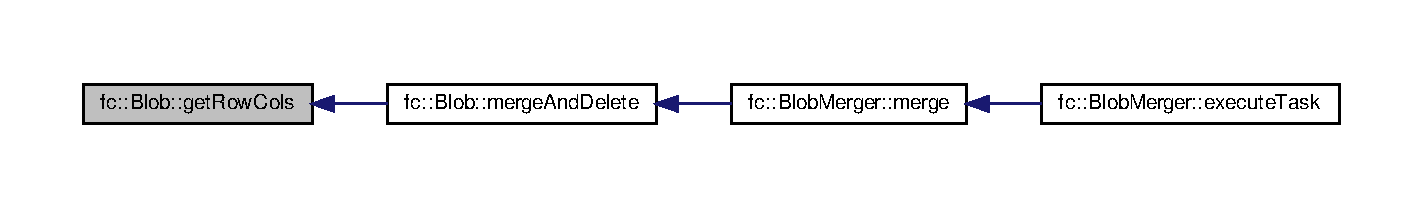
\includegraphics[width=350pt]{d2/d7e/classfc_1_1Blob_a80e63b761ebffdf90dea47b8a59b2c32_icgraph}
\end{center}
\end{figure}
\mbox{\Hypertarget{classfc_1_1Blob_af4a030b9ba08fd02242137a296a3692b}\label{classfc_1_1Blob_af4a030b9ba08fd02242137a296a3692b}} 
\index{fc\+::\+Blob@{fc\+::\+Blob}!get\+Row\+Max@{get\+Row\+Max}}
\index{get\+Row\+Max@{get\+Row\+Max}!fc\+::\+Blob@{fc\+::\+Blob}}
\subsubsection{\texorpdfstring{get\+Row\+Max()}{getRowMax()}}
{\footnotesize\ttfamily int32\+\_\+t fc\+::\+Blob\+::get\+Row\+Max (\begin{DoxyParamCaption}{ }\end{DoxyParamCaption}) const\hspace{0.3cm}{\ttfamily [inline]}}



Get maximum bounding box row. 

\begin{DoxyReturn}{Returns}
Maximum bounding box row 
\end{DoxyReturn}


Definition at line 102 of file Blob.\+h.

Here is the caller graph for this function\+:
\nopagebreak
\begin{figure}[H]
\begin{center}
\leavevmode
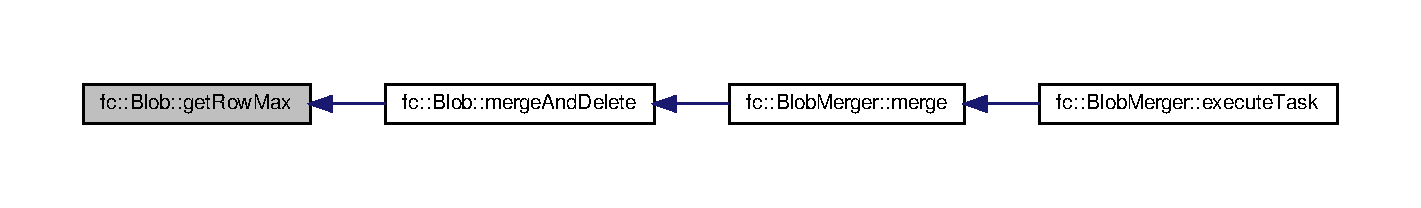
\includegraphics[width=350pt]{d2/d7e/classfc_1_1Blob_af4a030b9ba08fd02242137a296a3692b_icgraph}
\end{center}
\end{figure}
\mbox{\Hypertarget{classfc_1_1Blob_a167b6c3a33f301a7dcb527b289dd0834}\label{classfc_1_1Blob_a167b6c3a33f301a7dcb527b289dd0834}} 
\index{fc\+::\+Blob@{fc\+::\+Blob}!get\+Row\+Min@{get\+Row\+Min}}
\index{get\+Row\+Min@{get\+Row\+Min}!fc\+::\+Blob@{fc\+::\+Blob}}
\subsubsection{\texorpdfstring{get\+Row\+Min()}{getRowMin()}}
{\footnotesize\ttfamily int32\+\_\+t fc\+::\+Blob\+::get\+Row\+Min (\begin{DoxyParamCaption}{ }\end{DoxyParamCaption}) const\hspace{0.3cm}{\ttfamily [inline]}}



Get minimum bounding box row. 

\begin{DoxyReturn}{Returns}
Minimum bounding box row 
\end{DoxyReturn}


Definition at line 98 of file Blob.\+h.

Here is the caller graph for this function\+:
\nopagebreak
\begin{figure}[H]
\begin{center}
\leavevmode
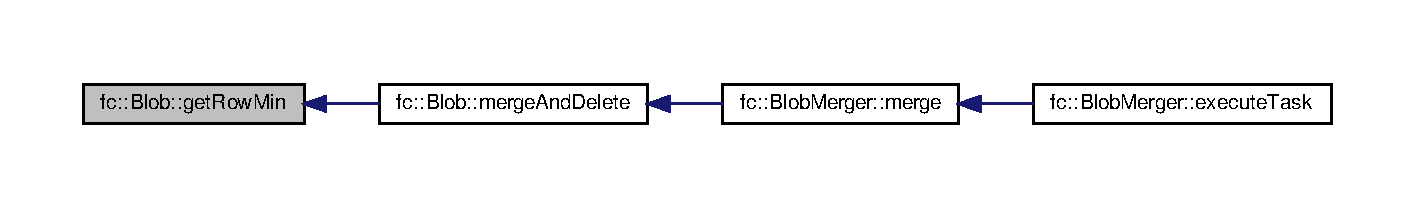
\includegraphics[width=350pt]{d2/d7e/classfc_1_1Blob_a167b6c3a33f301a7dcb527b289dd0834_icgraph}
\end{center}
\end{figure}
\mbox{\Hypertarget{classfc_1_1Blob_aeb84112e584a5e918530690b42cfd8f6}\label{classfc_1_1Blob_aeb84112e584a5e918530690b42cfd8f6}} 
\index{fc\+::\+Blob@{fc\+::\+Blob}!get\+Tag@{get\+Tag}}
\index{get\+Tag@{get\+Tag}!fc\+::\+Blob@{fc\+::\+Blob}}
\subsubsection{\texorpdfstring{get\+Tag()}{getTag()}}
{\footnotesize\ttfamily uint32\+\_\+t fc\+::\+Blob\+::get\+Tag (\begin{DoxyParamCaption}{ }\end{DoxyParamCaption}) const\hspace{0.3cm}{\ttfamily [inline]}}



Get \hyperlink{classfc_1_1Blob}{Blob} tag. 

\begin{DoxyReturn}{Returns}
\hyperlink{classfc_1_1Blob}{Blob} tag 
\end{DoxyReturn}


Definition at line 88 of file Blob.\+h.

\mbox{\Hypertarget{classfc_1_1Blob_a462ba30be4256cccc0270ab0d278bb07}\label{classfc_1_1Blob_a462ba30be4256cccc0270ab0d278bb07}} 
\index{fc\+::\+Blob@{fc\+::\+Blob}!is\+Pixelin\+Feature@{is\+Pixelin\+Feature}}
\index{is\+Pixelin\+Feature@{is\+Pixelin\+Feature}!fc\+::\+Blob@{fc\+::\+Blob}}
\subsubsection{\texorpdfstring{is\+Pixelin\+Feature()}{isPixelinFeature()}}
{\footnotesize\ttfamily bool fc\+::\+Blob\+::is\+Pixelin\+Feature (\begin{DoxyParamCaption}\item[{int32\+\_\+t}]{row,  }\item[{int32\+\_\+t}]{col }\end{DoxyParamCaption})\hspace{0.3cm}{\ttfamily [inline]}}



Test if a pixel is in a blob. 


\begin{DoxyParams}{Parameters}
{\em row} & Row asked \\
\hline
{\em col} & Col asked \\
\hline
\end{DoxyParams}
\begin{DoxyReturn}{Returns}
True is the pixel(row, col) is in the blob, else False 
\end{DoxyReturn}


Definition at line 128 of file Blob.\+h.

\mbox{\Hypertarget{classfc_1_1Blob_ae84692d9e132dd046b56bb6ac06dd8bb}\label{classfc_1_1Blob_ae84692d9e132dd046b56bb6ac06dd8bb}} 
\index{fc\+::\+Blob@{fc\+::\+Blob}!merge\+And\+Delete@{merge\+And\+Delete}}
\index{merge\+And\+Delete@{merge\+And\+Delete}!fc\+::\+Blob@{fc\+::\+Blob}}
\subsubsection{\texorpdfstring{merge\+And\+Delete()}{mergeAndDelete()}}
{\footnotesize\ttfamily \hyperlink{classfc_1_1Blob}{Blob}$\ast$ fc\+::\+Blob\+::merge\+And\+Delete (\begin{DoxyParamCaption}\item[{\hyperlink{classfc_1_1Blob}{Blob} $\ast$}]{blob }\end{DoxyParamCaption})\hspace{0.3cm}{\ttfamily [inline]}}



Merge 2 blobs, and delete the unused one. 


\begin{DoxyParams}{Parameters}
{\em blob} & \hyperlink{classfc_1_1Blob}{Blob} to merge with the current \\
\hline
\end{DoxyParams}
\begin{DoxyReturn}{Returns}
The blob merged 
\end{DoxyReturn}


Definition at line 186 of file Blob.\+h.

Here is the call graph for this function\+:
\nopagebreak
\begin{figure}[H]
\begin{center}
\leavevmode
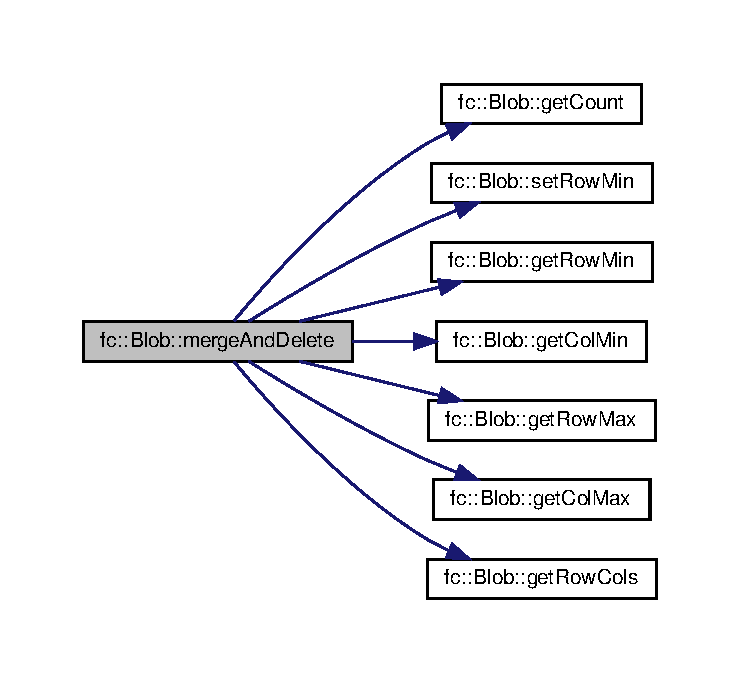
\includegraphics[width=350pt]{d2/d7e/classfc_1_1Blob_ae84692d9e132dd046b56bb6ac06dd8bb_cgraph}
\end{center}
\end{figure}
Here is the caller graph for this function\+:
\nopagebreak
\begin{figure}[H]
\begin{center}
\leavevmode
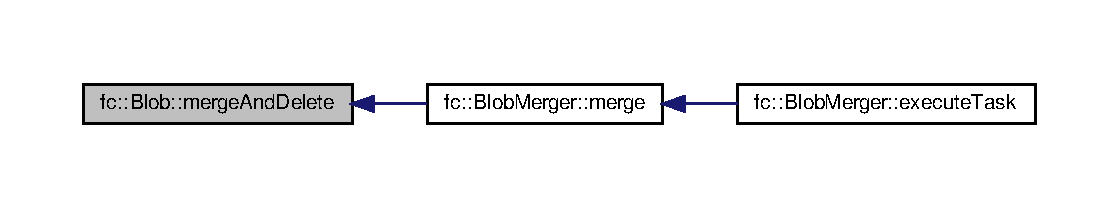
\includegraphics[width=350pt]{d2/d7e/classfc_1_1Blob_ae84692d9e132dd046b56bb6ac06dd8bb_icgraph}
\end{center}
\end{figure}
\mbox{\Hypertarget{classfc_1_1Blob_a0534b6d033d5dc27f24f7f7776b148c0}\label{classfc_1_1Blob_a0534b6d033d5dc27f24f7f7776b148c0}} 
\index{fc\+::\+Blob@{fc\+::\+Blob}!set\+Col\+Max@{set\+Col\+Max}}
\index{set\+Col\+Max@{set\+Col\+Max}!fc\+::\+Blob@{fc\+::\+Blob}}
\subsubsection{\texorpdfstring{set\+Col\+Max()}{setColMax()}}
{\footnotesize\ttfamily void fc\+::\+Blob\+::set\+Col\+Max (\begin{DoxyParamCaption}\item[{int32\+\_\+t}]{col\+Max }\end{DoxyParamCaption})\hspace{0.3cm}{\ttfamily [inline]}}



Maximum bounding box col setter. 


\begin{DoxyParams}{Parameters}
{\em col\+Max} & Maximum bounding box col \\
\hline
\end{DoxyParams}


Definition at line 153 of file Blob.\+h.

\mbox{\Hypertarget{classfc_1_1Blob_aa9972e1dd32aa399426b87bc4c610d69}\label{classfc_1_1Blob_aa9972e1dd32aa399426b87bc4c610d69}} 
\index{fc\+::\+Blob@{fc\+::\+Blob}!set\+Col\+Min@{set\+Col\+Min}}
\index{set\+Col\+Min@{set\+Col\+Min}!fc\+::\+Blob@{fc\+::\+Blob}}
\subsubsection{\texorpdfstring{set\+Col\+Min()}{setColMin()}}
{\footnotesize\ttfamily void fc\+::\+Blob\+::set\+Col\+Min (\begin{DoxyParamCaption}\item[{int32\+\_\+t}]{col\+Min }\end{DoxyParamCaption})\hspace{0.3cm}{\ttfamily [inline]}}



Minimum bounding box col setter. 


\begin{DoxyParams}{Parameters}
{\em col\+Min} & Minimum bounding box col \\
\hline
\end{DoxyParams}


Definition at line 149 of file Blob.\+h.

\mbox{\Hypertarget{classfc_1_1Blob_a4f404eafaf95bd017eecfbd234eb650e}\label{classfc_1_1Blob_a4f404eafaf95bd017eecfbd234eb650e}} 
\index{fc\+::\+Blob@{fc\+::\+Blob}!set\+Count@{set\+Count}}
\index{set\+Count@{set\+Count}!fc\+::\+Blob@{fc\+::\+Blob}}
\subsubsection{\texorpdfstring{set\+Count()}{setCount()}}
{\footnotesize\ttfamily void fc\+::\+Blob\+::set\+Count (\begin{DoxyParamCaption}\item[{uint64\+\_\+t}]{count }\end{DoxyParamCaption})\hspace{0.3cm}{\ttfamily [inline]}}



Count setter. 


\begin{DoxyParams}{Parameters}
{\em count} & Pixel Count \\
\hline
\end{DoxyParams}


Definition at line 157 of file Blob.\+h.

\mbox{\Hypertarget{classfc_1_1Blob_a88b9a5ef4d1ea26fd9e313b8d033d721}\label{classfc_1_1Blob_a88b9a5ef4d1ea26fd9e313b8d033d721}} 
\index{fc\+::\+Blob@{fc\+::\+Blob}!set\+Parent@{set\+Parent}}
\index{set\+Parent@{set\+Parent}!fc\+::\+Blob@{fc\+::\+Blob}}
\subsubsection{\texorpdfstring{set\+Parent()}{setParent()}}
{\footnotesize\ttfamily void fc\+::\+Blob\+::set\+Parent (\begin{DoxyParamCaption}\item[{\hyperlink{classfc_1_1Blob}{Blob} $\ast$}]{parent }\end{DoxyParamCaption})\hspace{0.3cm}{\ttfamily [inline]}}



\hyperlink{classfc_1_1Blob}{Blob} parent setter Used by Union find algorithm. 


\begin{DoxyParams}{Parameters}
{\em parent} & \hyperlink{classfc_1_1Blob}{Blob} parent \\
\hline
\end{DoxyParams}


Definition at line 161 of file Blob.\+h.

\mbox{\Hypertarget{classfc_1_1Blob_a21fdbcaf66775d27bb7680402fe2fd8a}\label{classfc_1_1Blob_a21fdbcaf66775d27bb7680402fe2fd8a}} 
\index{fc\+::\+Blob@{fc\+::\+Blob}!set\+Rank@{set\+Rank}}
\index{set\+Rank@{set\+Rank}!fc\+::\+Blob@{fc\+::\+Blob}}
\subsubsection{\texorpdfstring{set\+Rank()}{setRank()}}
{\footnotesize\ttfamily void fc\+::\+Blob\+::set\+Rank (\begin{DoxyParamCaption}\item[{uint32\+\_\+t}]{rank }\end{DoxyParamCaption})\hspace{0.3cm}{\ttfamily [inline]}}



\hyperlink{classfc_1_1Blob}{Blob} rank setter Used by Union find algorithm. 


\begin{DoxyParams}{Parameters}
{\em rank} & \hyperlink{classfc_1_1Blob}{Blob} rank \\
\hline
\end{DoxyParams}


Definition at line 165 of file Blob.\+h.

\mbox{\Hypertarget{classfc_1_1Blob_af726d6434723c76d5c9e793a99a01408}\label{classfc_1_1Blob_af726d6434723c76d5c9e793a99a01408}} 
\index{fc\+::\+Blob@{fc\+::\+Blob}!set\+Row\+Max@{set\+Row\+Max}}
\index{set\+Row\+Max@{set\+Row\+Max}!fc\+::\+Blob@{fc\+::\+Blob}}
\subsubsection{\texorpdfstring{set\+Row\+Max()}{setRowMax()}}
{\footnotesize\ttfamily void fc\+::\+Blob\+::set\+Row\+Max (\begin{DoxyParamCaption}\item[{int32\+\_\+t}]{row\+Max }\end{DoxyParamCaption})\hspace{0.3cm}{\ttfamily [inline]}}



Maximum bounding box row setter. 


\begin{DoxyParams}{Parameters}
{\em row\+Max} & Maximum bounding box row \\
\hline
\end{DoxyParams}


Definition at line 145 of file Blob.\+h.

\mbox{\Hypertarget{classfc_1_1Blob_a14a42d0f0fe5a8c06444609027faecbe}\label{classfc_1_1Blob_a14a42d0f0fe5a8c06444609027faecbe}} 
\index{fc\+::\+Blob@{fc\+::\+Blob}!set\+Row\+Min@{set\+Row\+Min}}
\index{set\+Row\+Min@{set\+Row\+Min}!fc\+::\+Blob@{fc\+::\+Blob}}
\subsubsection{\texorpdfstring{set\+Row\+Min()}{setRowMin()}}
{\footnotesize\ttfamily void fc\+::\+Blob\+::set\+Row\+Min (\begin{DoxyParamCaption}\item[{int32\+\_\+t}]{row\+Min }\end{DoxyParamCaption})\hspace{0.3cm}{\ttfamily [inline]}}



Minimum bounding box row setter. 


\begin{DoxyParams}{Parameters}
{\em row\+Min} & Minimum bounding box row \\
\hline
\end{DoxyParams}


Definition at line 141 of file Blob.\+h.

Here is the caller graph for this function\+:
\nopagebreak
\begin{figure}[H]
\begin{center}
\leavevmode
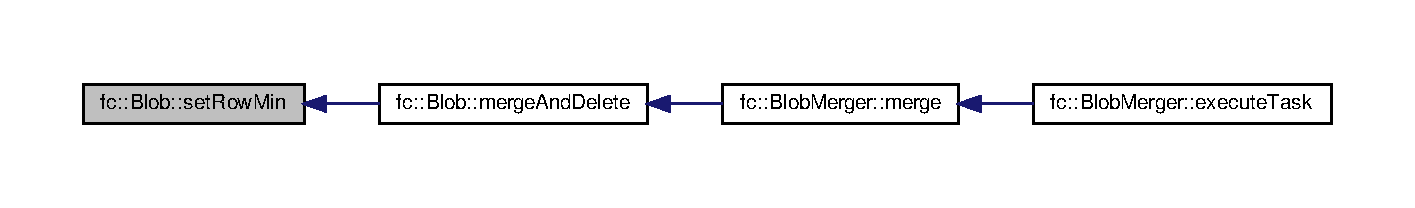
\includegraphics[width=350pt]{d2/d7e/classfc_1_1Blob_a14a42d0f0fe5a8c06444609027faecbe_icgraph}
\end{center}
\end{figure}


\subsection{Friends And Related Function Documentation}
\mbox{\Hypertarget{classfc_1_1Blob_a5fe38c43bc6a7886e8760e7b00ade43a}\label{classfc_1_1Blob_a5fe38c43bc6a7886e8760e7b00ade43a}} 
\index{fc\+::\+Blob@{fc\+::\+Blob}!operator$<$$<$@{operator$<$$<$}}
\index{operator$<$$<$@{operator$<$$<$}!fc\+::\+Blob@{fc\+::\+Blob}}
\subsubsection{\texorpdfstring{operator$<$$<$}{operator<<}}
{\footnotesize\ttfamily std\+::ostream\& operator$<$$<$ (\begin{DoxyParamCaption}\item[{std\+::ostream \&}]{os,  }\item[{const \hyperlink{classfc_1_1Blob}{Blob} \&}]{blob }\end{DoxyParamCaption})\hspace{0.3cm}{\ttfamily [friend]}}



Print blob state. 


\begin{DoxyParams}{Parameters}
{\em os} & Output stream \\
\hline
{\em blob} & \hyperlink{classfc_1_1Blob}{Blob} to print \\
\hline
\end{DoxyParams}
\begin{DoxyReturn}{Returns}
Output stream with the blob information 
\end{DoxyReturn}


Definition at line 230 of file Blob.\+h.



\subsection{Member Data Documentation}
\mbox{\Hypertarget{classfc_1_1Blob_ab35bcad8687bcbd04b0a7952702a88a6}\label{classfc_1_1Blob_ab35bcad8687bcbd04b0a7952702a88a6}} 
\index{fc\+::\+Blob@{fc\+::\+Blob}!\+\_\+col\+Max@{\+\_\+col\+Max}}
\index{\+\_\+col\+Max@{\+\_\+col\+Max}!fc\+::\+Blob@{fc\+::\+Blob}}
\subsubsection{\texorpdfstring{\+\_\+col\+Max}{\_colMax}}
{\footnotesize\ttfamily int32\+\_\+t fc\+::\+Blob\+::\+\_\+col\+Max \{\}\hspace{0.3cm}{\ttfamily [private]}}



Maximum bounding box col. 



Definition at line 256 of file Blob.\+h.

\mbox{\Hypertarget{classfc_1_1Blob_aa962a217328b361385584042e8d29eb9}\label{classfc_1_1Blob_aa962a217328b361385584042e8d29eb9}} 
\index{fc\+::\+Blob@{fc\+::\+Blob}!\+\_\+col\+Min@{\+\_\+col\+Min}}
\index{\+\_\+col\+Min@{\+\_\+col\+Min}!fc\+::\+Blob@{fc\+::\+Blob}}
\subsubsection{\texorpdfstring{\+\_\+col\+Min}{\_colMin}}
{\footnotesize\ttfamily int32\+\_\+t fc\+::\+Blob\+::\+\_\+col\+Min \{\}\hspace{0.3cm}{\ttfamily [private]}}



Minimum bounding box col. 



Definition at line 255 of file Blob.\+h.

\mbox{\Hypertarget{classfc_1_1Blob_a7a36fdbf8d1c967b0664613f1b7f3a98}\label{classfc_1_1Blob_a7a36fdbf8d1c967b0664613f1b7f3a98}} 
\index{fc\+::\+Blob@{fc\+::\+Blob}!\+\_\+count@{\+\_\+count}}
\index{\+\_\+count@{\+\_\+count}!fc\+::\+Blob@{fc\+::\+Blob}}
\subsubsection{\texorpdfstring{\+\_\+count}{\_count}}
{\footnotesize\ttfamily uint64\+\_\+t fc\+::\+Blob\+::\+\_\+count \{\}\hspace{0.3cm}{\ttfamily [private]}}



Number of pixel to fastened the blob merge. 



Definition at line 259 of file Blob.\+h.

\mbox{\Hypertarget{classfc_1_1Blob_ab58442d32a4ce2e9d5c4718d63e126d8}\label{classfc_1_1Blob_ab58442d32a4ce2e9d5c4718d63e126d8}} 
\index{fc\+::\+Blob@{fc\+::\+Blob}!\+\_\+parent@{\+\_\+parent}}
\index{\+\_\+parent@{\+\_\+parent}!fc\+::\+Blob@{fc\+::\+Blob}}
\subsubsection{\texorpdfstring{\+\_\+parent}{\_parent}}
{\footnotesize\ttfamily \hyperlink{classfc_1_1Blob}{Blob}$\ast$ fc\+::\+Blob\+::\+\_\+parent = nullptr\hspace{0.3cm}{\ttfamily [private]}}



\hyperlink{classfc_1_1Blob}{Blob} parent, used by the Union find algorithm. 



Definition at line 246 of file Blob.\+h.

\mbox{\Hypertarget{classfc_1_1Blob_ad19347abbefa18b6e98e1156cf09fe3a}\label{classfc_1_1Blob_ad19347abbefa18b6e98e1156cf09fe3a}} 
\index{fc\+::\+Blob@{fc\+::\+Blob}!\+\_\+rank@{\+\_\+rank}}
\index{\+\_\+rank@{\+\_\+rank}!fc\+::\+Blob@{fc\+::\+Blob}}
\subsubsection{\texorpdfstring{\+\_\+rank}{\_rank}}
{\footnotesize\ttfamily uint32\+\_\+t fc\+::\+Blob\+::\+\_\+rank = 0\hspace{0.3cm}{\ttfamily [private]}}



\hyperlink{classfc_1_1Blob}{Blob} rank, used by the Union find algorithm. 



Definition at line 249 of file Blob.\+h.

\mbox{\Hypertarget{classfc_1_1Blob_a2688a4b64b2e3d37e7309aca03177b55}\label{classfc_1_1Blob_a2688a4b64b2e3d37e7309aca03177b55}} 
\index{fc\+::\+Blob@{fc\+::\+Blob}!\+\_\+row\+Cols@{\+\_\+row\+Cols}}
\index{\+\_\+row\+Cols@{\+\_\+row\+Cols}!fc\+::\+Blob@{fc\+::\+Blob}}
\subsubsection{\texorpdfstring{\+\_\+row\+Cols}{\_rowCols}}
{\footnotesize\ttfamily std\+::unordered\+\_\+map$<$int32\+\_\+t, std\+::unordered\+\_\+set$<$int32\+\_\+t$>$ $>$ fc\+::\+Blob\+::\+\_\+row\+Cols \{\}\hspace{0.3cm}{\ttfamily [private]}}



Sparse matrix of unique coordinates composing the blob. 



Definition at line 263 of file Blob.\+h.

\mbox{\Hypertarget{classfc_1_1Blob_ada6057ee4bf33c0a432f28d5d42413dd}\label{classfc_1_1Blob_ada6057ee4bf33c0a432f28d5d42413dd}} 
\index{fc\+::\+Blob@{fc\+::\+Blob}!\+\_\+row\+Max@{\+\_\+row\+Max}}
\index{\+\_\+row\+Max@{\+\_\+row\+Max}!fc\+::\+Blob@{fc\+::\+Blob}}
\subsubsection{\texorpdfstring{\+\_\+row\+Max}{\_rowMax}}
{\footnotesize\ttfamily int32\+\_\+t fc\+::\+Blob\+::\+\_\+row\+Max \{\}\hspace{0.3cm}{\ttfamily [private]}}



Maximum bounding box row. 



Definition at line 254 of file Blob.\+h.

\mbox{\Hypertarget{classfc_1_1Blob_ab63888a3d59cb3b81ad10e19864b101a}\label{classfc_1_1Blob_ab63888a3d59cb3b81ad10e19864b101a}} 
\index{fc\+::\+Blob@{fc\+::\+Blob}!\+\_\+row\+Min@{\+\_\+row\+Min}}
\index{\+\_\+row\+Min@{\+\_\+row\+Min}!fc\+::\+Blob@{fc\+::\+Blob}}
\subsubsection{\texorpdfstring{\+\_\+row\+Min}{\_rowMin}}
{\footnotesize\ttfamily int32\+\_\+t fc\+::\+Blob\+::\+\_\+row\+Min \{\}\hspace{0.3cm}{\ttfamily [private]}}



Minimum bounding box row. 



Definition at line 253 of file Blob.\+h.

\mbox{\Hypertarget{classfc_1_1Blob_af07e1270217289a0879386f267bf5fe5}\label{classfc_1_1Blob_af07e1270217289a0879386f267bf5fe5}} 
\index{fc\+::\+Blob@{fc\+::\+Blob}!\+\_\+tag@{\+\_\+tag}}
\index{\+\_\+tag@{\+\_\+tag}!fc\+::\+Blob@{fc\+::\+Blob}}
\subsubsection{\texorpdfstring{\+\_\+tag}{\_tag}}
{\footnotesize\ttfamily uint32\+\_\+t fc\+::\+Blob\+::\+\_\+tag = 0\hspace{0.3cm}{\ttfamily [private]}}



Tag, only used to print/debug purpose. 



Definition at line 250 of file Blob.\+h.



The documentation for this class was generated from the following file\+:\begin{DoxyCompactItemize}
\item 
/home/anb22/\+Documents/\+Fast-\/\+Image/\+Fast\+Image/src/\+Fast\+Image/\+Feature\+Collection/\+Data/\hyperlink{Blob_8h}{Blob.\+h}\end{DoxyCompactItemize}

\hypertarget{classfc_1_1BlobMerger}{}\section{fc\+:\+:Blob\+Merger Class Reference}
\label{classfc_1_1BlobMerger}\index{fc\+::\+Blob\+Merger@{fc\+::\+Blob\+Merger}}


Merges multiple \hyperlink{classfc_1_1ViewAnalyse}{fc\+::\+View\+Analyse} to build the \hyperlink{classfc_1_1Feature}{Feature} Collection.  




{\ttfamily \#include $<$Fast\+Image/\+Feature\+Collection/\+Tasks/\+Blob\+Merger.\+h$>$}



Inheritance diagram for fc\+:\+:Blob\+Merger\+:
\nopagebreak
\begin{figure}[H]
\begin{center}
\leavevmode
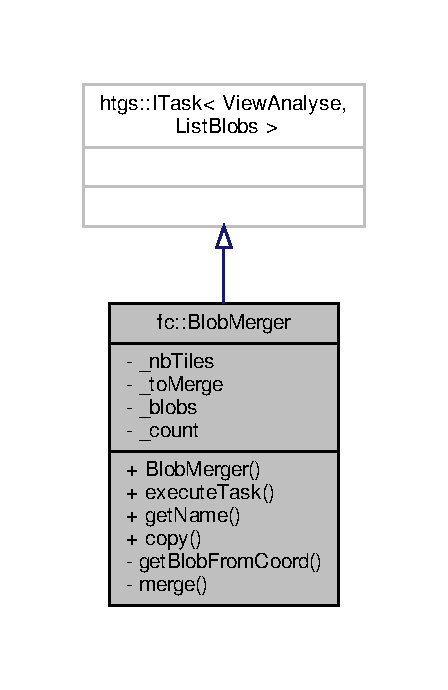
\includegraphics[width=215pt]{d1/d9d/classfc_1_1BlobMerger__inherit__graph}
\end{center}
\end{figure}


Collaboration diagram for fc\+:\+:Blob\+Merger\+:
\nopagebreak
\begin{figure}[H]
\begin{center}
\leavevmode
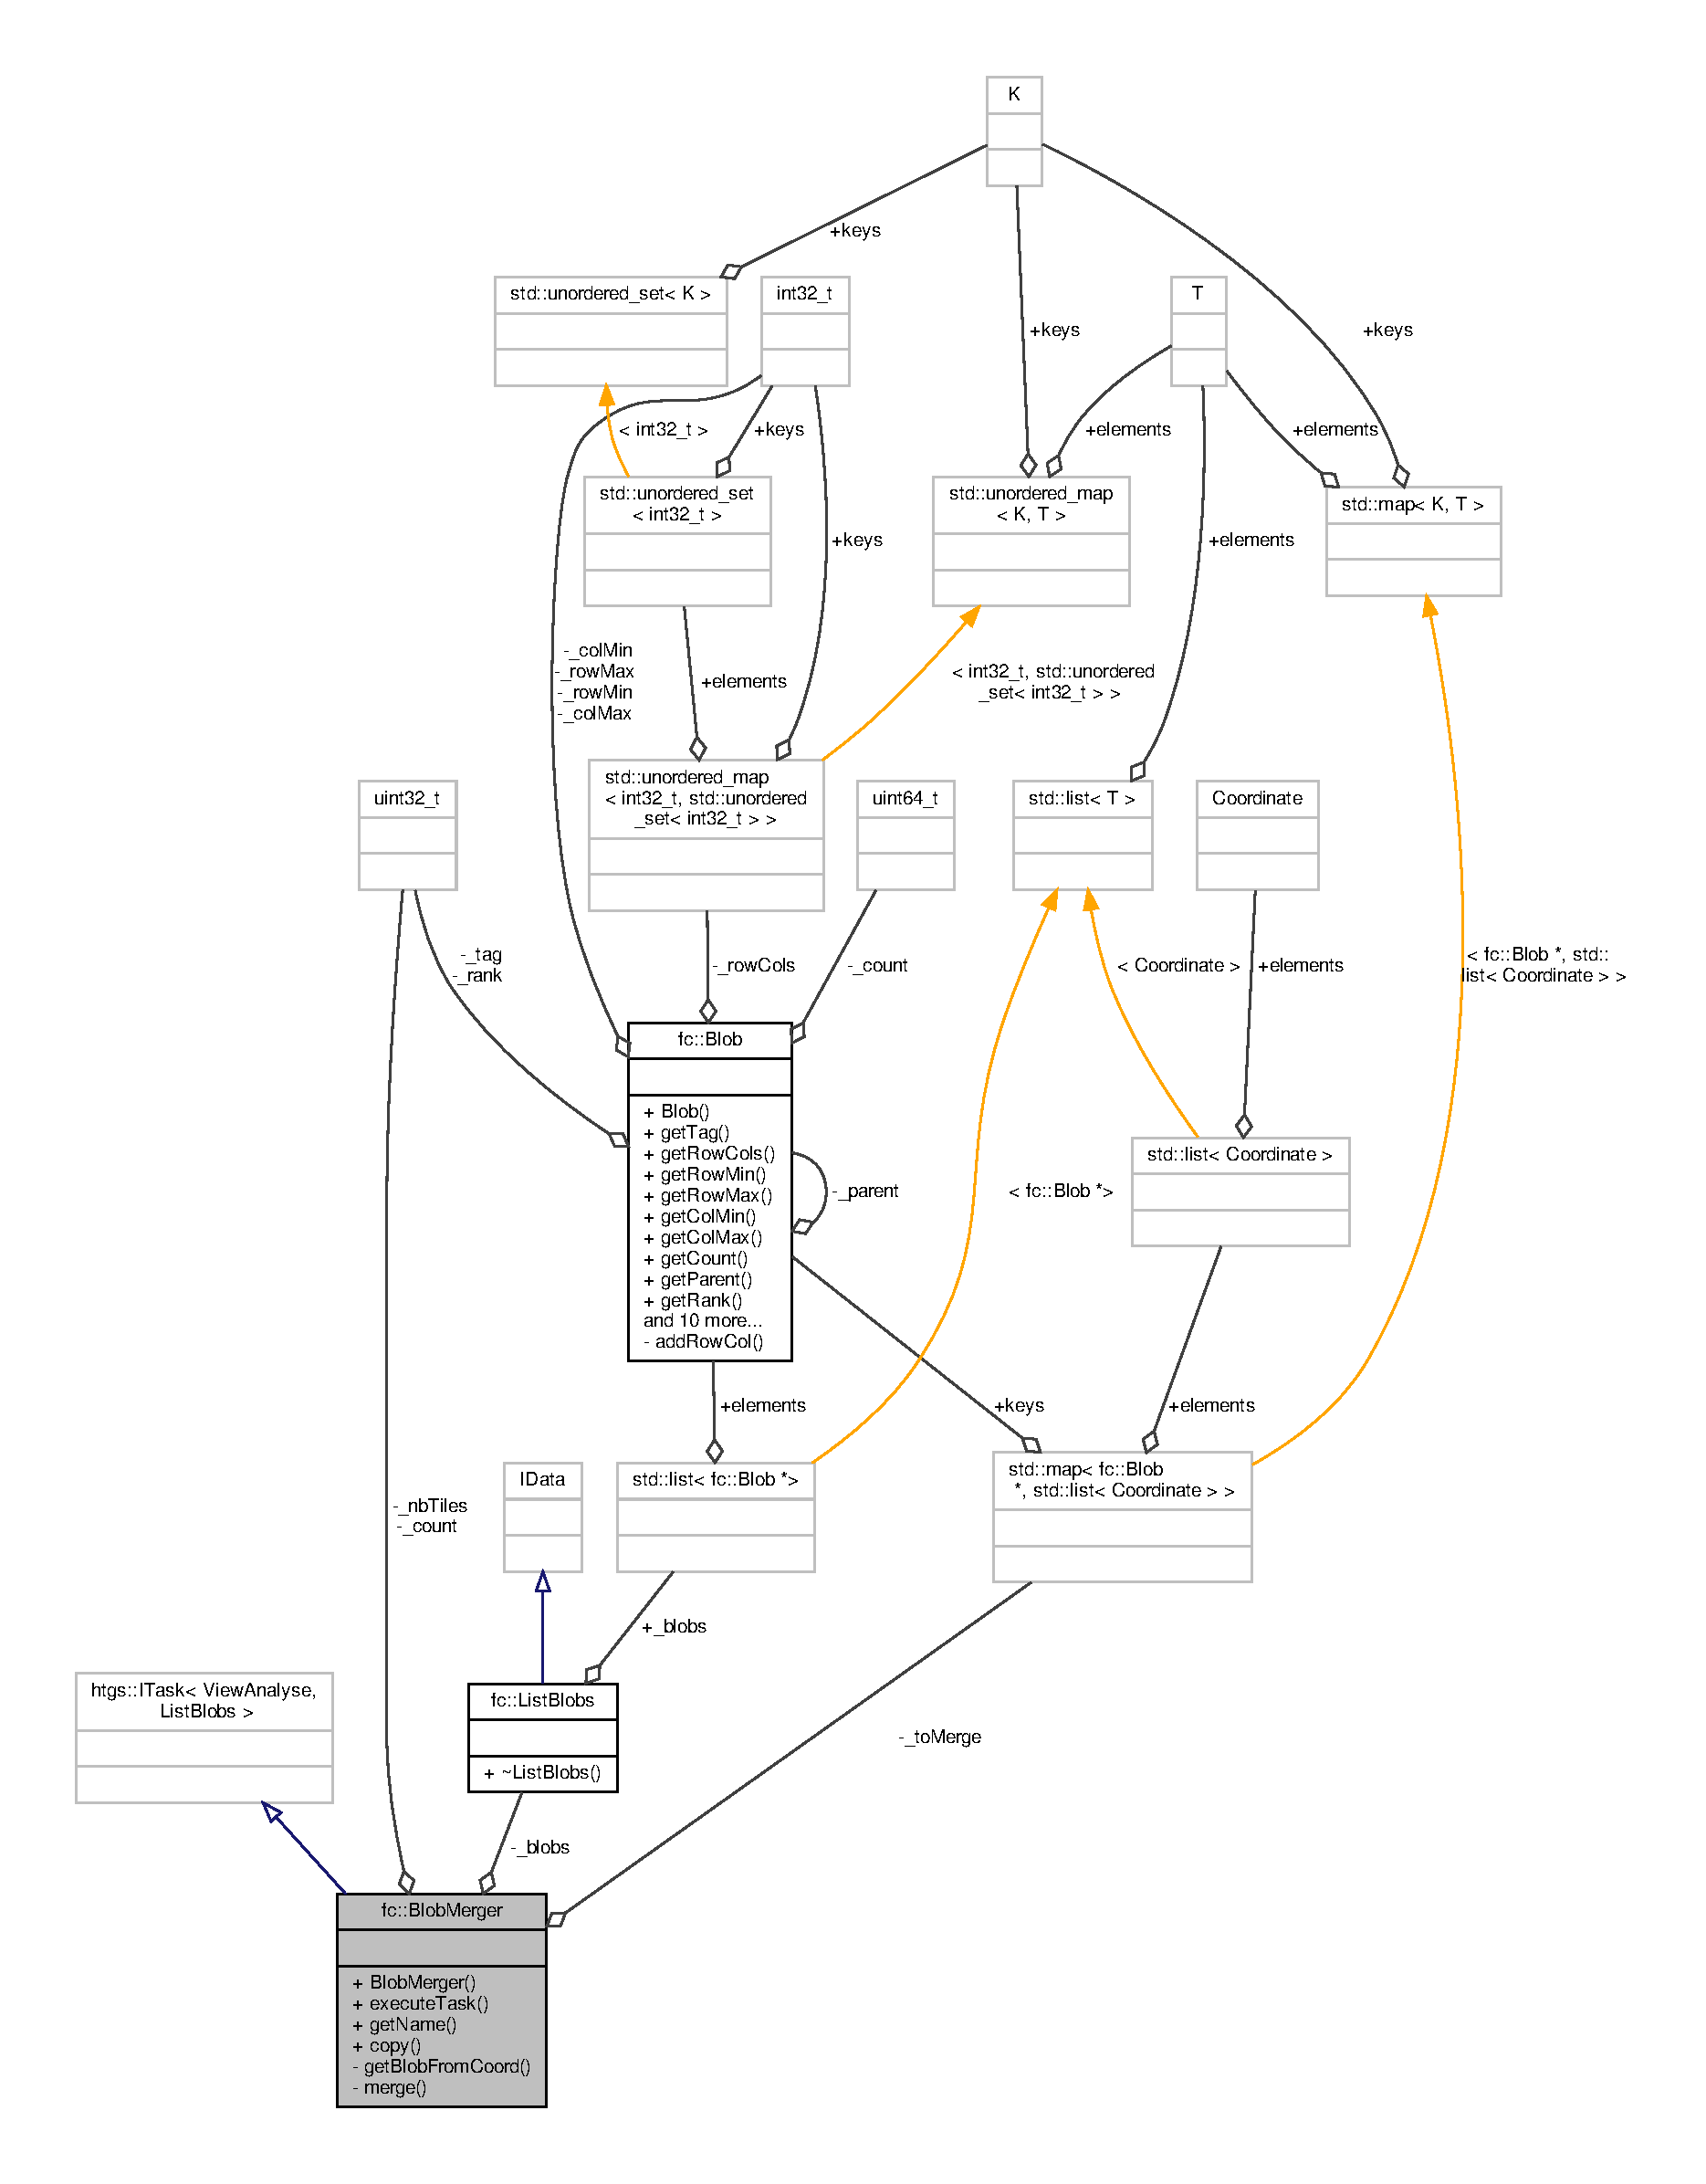
\includegraphics[width=350pt]{dd/d0c/classfc_1_1BlobMerger__coll__graph}
\end{center}
\end{figure}
\subsection*{Public Member Functions}
\begin{DoxyCompactItemize}
\item 
\hyperlink{classfc_1_1BlobMerger_a6304048cc051fa0401bb998b15bac73d}{Blob\+Merger} (uint32\+\_\+t image\+Height, uint32\+\_\+t image\+Width, uint32\+\_\+t nb\+Tiles)
\begin{DoxyCompactList}\small\item\em \hyperlink{classfc_1_1BlobMerger}{Blob\+Merger} constructor. \end{DoxyCompactList}\item 
void \hyperlink{classfc_1_1BlobMerger_a81af854864e9ae220ad7c5fed0eef195}{execute\+Task} (std\+::shared\+\_\+ptr$<$ \hyperlink{classfc_1_1ViewAnalyse}{View\+Analyse} $>$ data) override
\begin{DoxyCompactList}\small\item\em Get the view analyse, merge them into one analyse and merge all blob to build the feature collection. \end{DoxyCompactList}\item 
std\+::string \hyperlink{classfc_1_1BlobMerger_a5b14aeeae9e03ceee8fdd90d2828a1bb}{get\+Name} () override
\begin{DoxyCompactList}\small\item\em Get the name of the task. \end{DoxyCompactList}\item 
\hyperlink{classfc_1_1BlobMerger}{Blob\+Merger} $\ast$ \hyperlink{classfc_1_1BlobMerger_a71cdaa2d3b28253922f0e43d911003ca}{copy} () override
\begin{DoxyCompactList}\small\item\em Task copy, should be a singleton, to send bask itself. \end{DoxyCompactList}\end{DoxyCompactItemize}
\subsection*{Private Member Functions}
\begin{DoxyCompactItemize}
\item 
\hyperlink{classfc_1_1Blob}{Blob} $\ast$ \hyperlink{classfc_1_1BlobMerger_ac2e61560c60b1467e385a3d08577c650}{get\+Blob\+From\+Coord} (const int32\+\_\+t \&row, const int32\+\_\+t \&col) const
\begin{DoxyCompactList}\small\item\em Retrieve a blob from a coordinate, nullptr is to blob is corresponding. \end{DoxyCompactList}\item 
void \hyperlink{classfc_1_1BlobMerger_a11fa980b355aa46271460f33a5cce0ac}{merge} ()
\begin{DoxyCompactList}\small\item\em Merge all the blobs from all the view analyser. \end{DoxyCompactList}\end{DoxyCompactItemize}
\subsection*{Private Attributes}
\begin{DoxyCompactItemize}
\item 
uint32\+\_\+t \hyperlink{classfc_1_1BlobMerger_ad1b9d727d311831ea57e8f57161f8e13}{\+\_\+nb\+Tiles} = 0
\begin{DoxyCompactList}\small\item\em Images number of tiles. \end{DoxyCompactList}\item 
std\+::map$<$ \hyperlink{classfc_1_1Blob}{Blob} $\ast$, std\+::list$<$ \hyperlink{namespacefc_a7da125cb1e99553c27c07139ee8a62ca}{Coordinate} $>$ $>$ \hyperlink{classfc_1_1BlobMerger_a290bb3c28c7042b92761ec2a55f017dc}{\+\_\+to\+Merge} \{\}
\begin{DoxyCompactList}\small\item\em Merge structure. \end{DoxyCompactList}\item 
\hyperlink{structfc_1_1ListBlobs}{List\+Blobs} $\ast$ \hyperlink{classfc_1_1BlobMerger_a2754a886c8ef78537af5bd94e564cf55}{\+\_\+blobs}
\begin{DoxyCompactList}\small\item\em Blobs list. \end{DoxyCompactList}\item 
uint32\+\_\+t \hyperlink{classfc_1_1BlobMerger_abea5457da76db98d6a29dd06561d5bcf}{\+\_\+count} = 0
\begin{DoxyCompactList}\small\item\em Number of views analysed. \end{DoxyCompactList}\end{DoxyCompactItemize}


\subsection{Detailed Description}
Merges multiple \hyperlink{classfc_1_1ViewAnalyse}{fc\+::\+View\+Analyse} to build the \hyperlink{classfc_1_1Feature}{Feature} Collection. 

Merge the different analyse with a disjoint-\/set data structure to represent each blobs and merge them easily\+: \href{https://en.wikipedia.org/wiki/Disjoint-set_data_structure}{\tt https\+://en.\+wikipedia.\+org/wiki/\+Disjoint-\/set\+\_\+data\+\_\+structure} 

Definition at line 62 of file Blob\+Merger.\+h.



\subsection{Constructor \& Destructor Documentation}
\mbox{\Hypertarget{classfc_1_1BlobMerger_a6304048cc051fa0401bb998b15bac73d}\label{classfc_1_1BlobMerger_a6304048cc051fa0401bb998b15bac73d}} 
\index{fc\+::\+Blob\+Merger@{fc\+::\+Blob\+Merger}!Blob\+Merger@{Blob\+Merger}}
\index{Blob\+Merger@{Blob\+Merger}!fc\+::\+Blob\+Merger@{fc\+::\+Blob\+Merger}}
\subsubsection{\texorpdfstring{Blob\+Merger()}{BlobMerger()}}
{\footnotesize\ttfamily fc\+::\+Blob\+Merger\+::\+Blob\+Merger (\begin{DoxyParamCaption}\item[{uint32\+\_\+t}]{image\+Height,  }\item[{uint32\+\_\+t}]{image\+Width,  }\item[{uint32\+\_\+t}]{nb\+Tiles }\end{DoxyParamCaption})\hspace{0.3cm}{\ttfamily [inline]}}



\hyperlink{classfc_1_1BlobMerger}{Blob\+Merger} constructor. 


\begin{DoxyParams}{Parameters}
{\em image\+Height} & Image Height \\
\hline
{\em image\+Width} & Image\+Width \\
\hline
{\em nb\+Tiles} & Number of tiles in the image \\
\hline
\end{DoxyParams}


Definition at line 68 of file Blob\+Merger.\+h.



\subsection{Member Function Documentation}
\mbox{\Hypertarget{classfc_1_1BlobMerger_a71cdaa2d3b28253922f0e43d911003ca}\label{classfc_1_1BlobMerger_a71cdaa2d3b28253922f0e43d911003ca}} 
\index{fc\+::\+Blob\+Merger@{fc\+::\+Blob\+Merger}!copy@{copy}}
\index{copy@{copy}!fc\+::\+Blob\+Merger@{fc\+::\+Blob\+Merger}}
\subsubsection{\texorpdfstring{copy()}{copy()}}
{\footnotesize\ttfamily \hyperlink{classfc_1_1BlobMerger}{Blob\+Merger}$\ast$ fc\+::\+Blob\+Merger\+::copy (\begin{DoxyParamCaption}{ }\end{DoxyParamCaption})\hspace{0.3cm}{\ttfamily [inline]}, {\ttfamily [override]}}



Task copy, should be a singleton, to send bask itself. 

\begin{DoxyReturn}{Returns}
itself 
\end{DoxyReturn}


Definition at line 101 of file Blob\+Merger.\+h.

\mbox{\Hypertarget{classfc_1_1BlobMerger_a81af854864e9ae220ad7c5fed0eef195}\label{classfc_1_1BlobMerger_a81af854864e9ae220ad7c5fed0eef195}} 
\index{fc\+::\+Blob\+Merger@{fc\+::\+Blob\+Merger}!execute\+Task@{execute\+Task}}
\index{execute\+Task@{execute\+Task}!fc\+::\+Blob\+Merger@{fc\+::\+Blob\+Merger}}
\subsubsection{\texorpdfstring{execute\+Task()}{executeTask()}}
{\footnotesize\ttfamily void fc\+::\+Blob\+Merger\+::execute\+Task (\begin{DoxyParamCaption}\item[{std\+::shared\+\_\+ptr$<$ \hyperlink{classfc_1_1ViewAnalyse}{View\+Analyse} $>$}]{data }\end{DoxyParamCaption})\hspace{0.3cm}{\ttfamily [inline]}, {\ttfamily [override]}}



Get the view analyse, merge them into one analyse and merge all blob to build the feature collection. 


\begin{DoxyParams}{Parameters}
{\em data} & View analyse \\
\hline
\end{DoxyParams}


Definition at line 76 of file Blob\+Merger.\+h.

Here is the call graph for this function\+:
\nopagebreak
\begin{figure}[H]
\begin{center}
\leavevmode
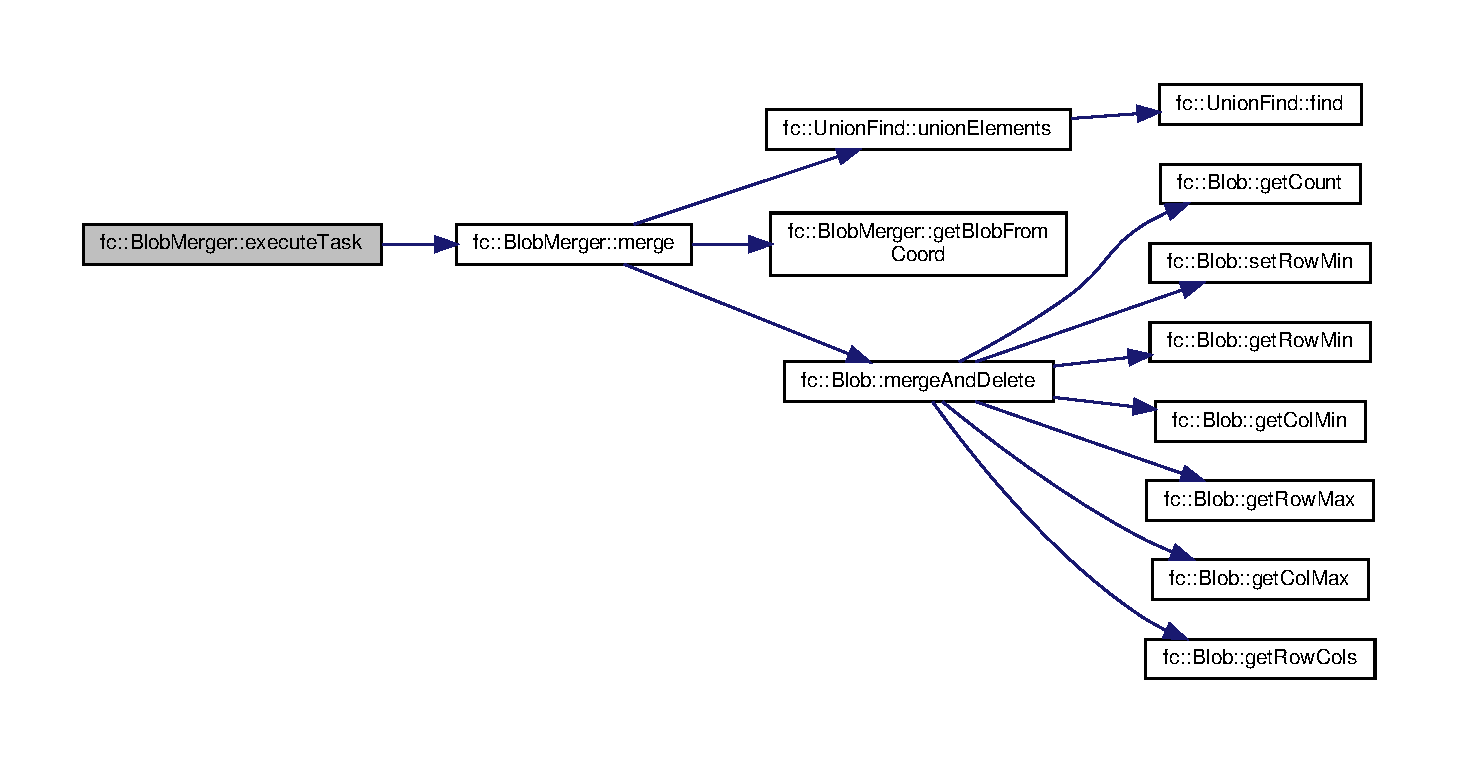
\includegraphics[width=350pt]{d3/df4/classfc_1_1BlobMerger_a81af854864e9ae220ad7c5fed0eef195_cgraph}
\end{center}
\end{figure}
\mbox{\Hypertarget{classfc_1_1BlobMerger_ac2e61560c60b1467e385a3d08577c650}\label{classfc_1_1BlobMerger_ac2e61560c60b1467e385a3d08577c650}} 
\index{fc\+::\+Blob\+Merger@{fc\+::\+Blob\+Merger}!get\+Blob\+From\+Coord@{get\+Blob\+From\+Coord}}
\index{get\+Blob\+From\+Coord@{get\+Blob\+From\+Coord}!fc\+::\+Blob\+Merger@{fc\+::\+Blob\+Merger}}
\subsubsection{\texorpdfstring{get\+Blob\+From\+Coord()}{getBlobFromCoord()}}
{\footnotesize\ttfamily \hyperlink{classfc_1_1Blob}{Blob}$\ast$ fc\+::\+Blob\+Merger\+::get\+Blob\+From\+Coord (\begin{DoxyParamCaption}\item[{const int32\+\_\+t \&}]{row,  }\item[{const int32\+\_\+t \&}]{col }\end{DoxyParamCaption}) const\hspace{0.3cm}{\ttfamily [inline]}, {\ttfamily [private]}}



Retrieve a blob from a coordinate, nullptr is to blob is corresponding. 


\begin{DoxyParams}{Parameters}
{\em row} & Row \\
\hline
{\em col} & Column \\
\hline
\end{DoxyParams}
\begin{DoxyReturn}{Returns}
True if a blob has been found, else False 
\end{DoxyReturn}


Definition at line 109 of file Blob\+Merger.\+h.

Here is the caller graph for this function\+:
\nopagebreak
\begin{figure}[H]
\begin{center}
\leavevmode
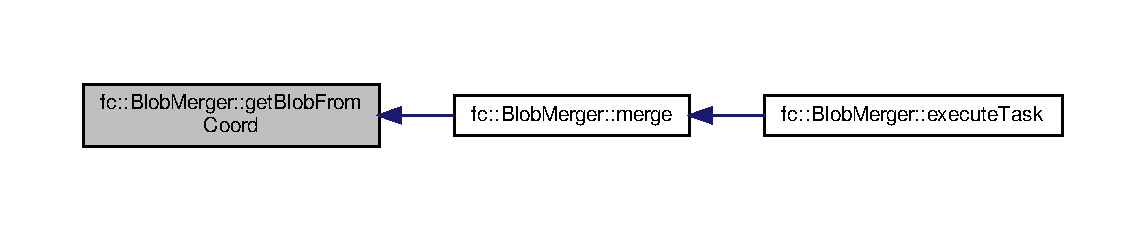
\includegraphics[width=350pt]{d3/df4/classfc_1_1BlobMerger_ac2e61560c60b1467e385a3d08577c650_icgraph}
\end{center}
\end{figure}
\mbox{\Hypertarget{classfc_1_1BlobMerger_a5b14aeeae9e03ceee8fdd90d2828a1bb}\label{classfc_1_1BlobMerger_a5b14aeeae9e03ceee8fdd90d2828a1bb}} 
\index{fc\+::\+Blob\+Merger@{fc\+::\+Blob\+Merger}!get\+Name@{get\+Name}}
\index{get\+Name@{get\+Name}!fc\+::\+Blob\+Merger@{fc\+::\+Blob\+Merger}}
\subsubsection{\texorpdfstring{get\+Name()}{getName()}}
{\footnotesize\ttfamily std\+::string fc\+::\+Blob\+Merger\+::get\+Name (\begin{DoxyParamCaption}{ }\end{DoxyParamCaption})\hspace{0.3cm}{\ttfamily [inline]}, {\ttfamily [override]}}



Get the name of the task. 

\begin{DoxyReturn}{Returns}
Task name 
\end{DoxyReturn}


Definition at line 97 of file Blob\+Merger.\+h.

\mbox{\Hypertarget{classfc_1_1BlobMerger_a11fa980b355aa46271460f33a5cce0ac}\label{classfc_1_1BlobMerger_a11fa980b355aa46271460f33a5cce0ac}} 
\index{fc\+::\+Blob\+Merger@{fc\+::\+Blob\+Merger}!merge@{merge}}
\index{merge@{merge}!fc\+::\+Blob\+Merger@{fc\+::\+Blob\+Merger}}
\subsubsection{\texorpdfstring{merge()}{merge()}}
{\footnotesize\ttfamily void fc\+::\+Blob\+Merger\+::merge (\begin{DoxyParamCaption}{ }\end{DoxyParamCaption})\hspace{0.3cm}{\ttfamily [inline]}, {\ttfamily [private]}}



Merge all the blobs from all the view analyser. 



Definition at line 121 of file Blob\+Merger.\+h.

Here is the call graph for this function\+:
\nopagebreak
\begin{figure}[H]
\begin{center}
\leavevmode
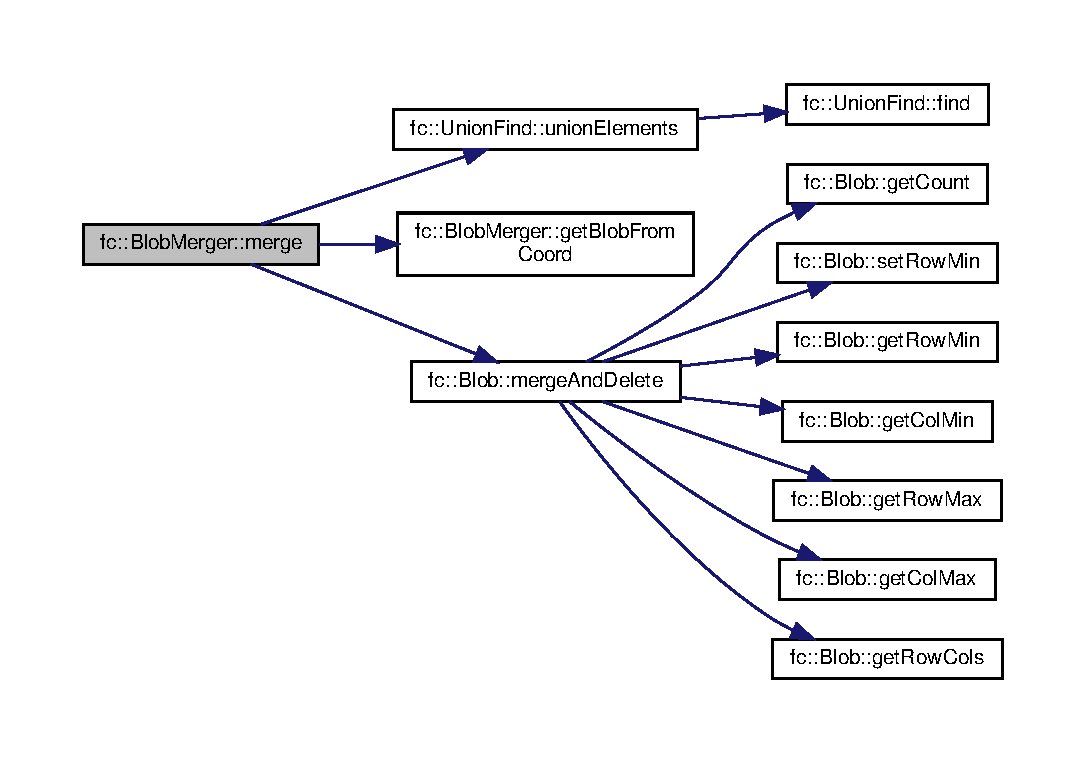
\includegraphics[width=350pt]{d3/df4/classfc_1_1BlobMerger_a11fa980b355aa46271460f33a5cce0ac_cgraph}
\end{center}
\end{figure}
Here is the caller graph for this function\+:
\nopagebreak
\begin{figure}[H]
\begin{center}
\leavevmode
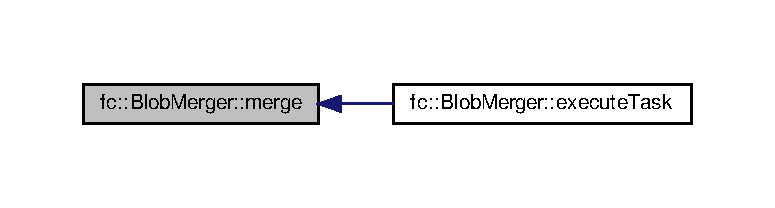
\includegraphics[width=350pt]{d3/df4/classfc_1_1BlobMerger_a11fa980b355aa46271460f33a5cce0ac_icgraph}
\end{center}
\end{figure}


\subsection{Member Data Documentation}
\mbox{\Hypertarget{classfc_1_1BlobMerger_a2754a886c8ef78537af5bd94e564cf55}\label{classfc_1_1BlobMerger_a2754a886c8ef78537af5bd94e564cf55}} 
\index{fc\+::\+Blob\+Merger@{fc\+::\+Blob\+Merger}!\+\_\+blobs@{\+\_\+blobs}}
\index{\+\_\+blobs@{\+\_\+blobs}!fc\+::\+Blob\+Merger@{fc\+::\+Blob\+Merger}}
\subsubsection{\texorpdfstring{\+\_\+blobs}{\_blobs}}
{\footnotesize\ttfamily \hyperlink{structfc_1_1ListBlobs}{List\+Blobs}$\ast$ fc\+::\+Blob\+Merger\+::\+\_\+blobs\hspace{0.3cm}{\ttfamily [private]}}



Blobs list. 



Definition at line 169 of file Blob\+Merger.\+h.

\mbox{\Hypertarget{classfc_1_1BlobMerger_abea5457da76db98d6a29dd06561d5bcf}\label{classfc_1_1BlobMerger_abea5457da76db98d6a29dd06561d5bcf}} 
\index{fc\+::\+Blob\+Merger@{fc\+::\+Blob\+Merger}!\+\_\+count@{\+\_\+count}}
\index{\+\_\+count@{\+\_\+count}!fc\+::\+Blob\+Merger@{fc\+::\+Blob\+Merger}}
\subsubsection{\texorpdfstring{\+\_\+count}{\_count}}
{\footnotesize\ttfamily uint32\+\_\+t fc\+::\+Blob\+Merger\+::\+\_\+count = 0\hspace{0.3cm}{\ttfamily [private]}}



Number of views analysed. 



Definition at line 172 of file Blob\+Merger.\+h.

\mbox{\Hypertarget{classfc_1_1BlobMerger_ad1b9d727d311831ea57e8f57161f8e13}\label{classfc_1_1BlobMerger_ad1b9d727d311831ea57e8f57161f8e13}} 
\index{fc\+::\+Blob\+Merger@{fc\+::\+Blob\+Merger}!\+\_\+nb\+Tiles@{\+\_\+nb\+Tiles}}
\index{\+\_\+nb\+Tiles@{\+\_\+nb\+Tiles}!fc\+::\+Blob\+Merger@{fc\+::\+Blob\+Merger}}
\subsubsection{\texorpdfstring{\+\_\+nb\+Tiles}{\_nbTiles}}
{\footnotesize\ttfamily uint32\+\_\+t fc\+::\+Blob\+Merger\+::\+\_\+nb\+Tiles = 0\hspace{0.3cm}{\ttfamily [private]}}



Images number of tiles. 



Definition at line 163 of file Blob\+Merger.\+h.

\mbox{\Hypertarget{classfc_1_1BlobMerger_a290bb3c28c7042b92761ec2a55f017dc}\label{classfc_1_1BlobMerger_a290bb3c28c7042b92761ec2a55f017dc}} 
\index{fc\+::\+Blob\+Merger@{fc\+::\+Blob\+Merger}!\+\_\+to\+Merge@{\+\_\+to\+Merge}}
\index{\+\_\+to\+Merge@{\+\_\+to\+Merge}!fc\+::\+Blob\+Merger@{fc\+::\+Blob\+Merger}}
\subsubsection{\texorpdfstring{\+\_\+to\+Merge}{\_toMerge}}
{\footnotesize\ttfamily std\+::map$<$\hyperlink{classfc_1_1Blob}{Blob} $\ast$, std\+::list$<$\hyperlink{namespacefc_a7da125cb1e99553c27c07139ee8a62ca}{Coordinate} $>$ $>$ fc\+::\+Blob\+Merger\+::\+\_\+to\+Merge \{\}\hspace{0.3cm}{\ttfamily [private]}}



Merge structure. 



Definition at line 166 of file Blob\+Merger.\+h.



The documentation for this class was generated from the following file\+:\begin{DoxyCompactItemize}
\item 
/home/anb22/\+Documents/\+Fast-\/\+Image/\+Fast\+Image/src/\+Fast\+Image/\+Feature\+Collection/\+Tasks/\hyperlink{BlobMerger_8h}{Blob\+Merger.\+h}\end{DoxyCompactItemize}

\hypertarget{classfc_1_1BoundingBox}{}\section{fc\+:\+:Bounding\+Box Class Reference}
\label{classfc_1_1BoundingBox}\index{fc\+::\+Bounding\+Box@{fc\+::\+Bounding\+Box}}


Define a bounding box around a feature.  




{\ttfamily \#include $<$Fast\+Image/\+Feature\+Collection/\+Bounding\+Box.\+h$>$}



Collaboration diagram for fc\+:\+:Bounding\+Box\+:
\nopagebreak
\begin{figure}[H]
\begin{center}
\leavevmode
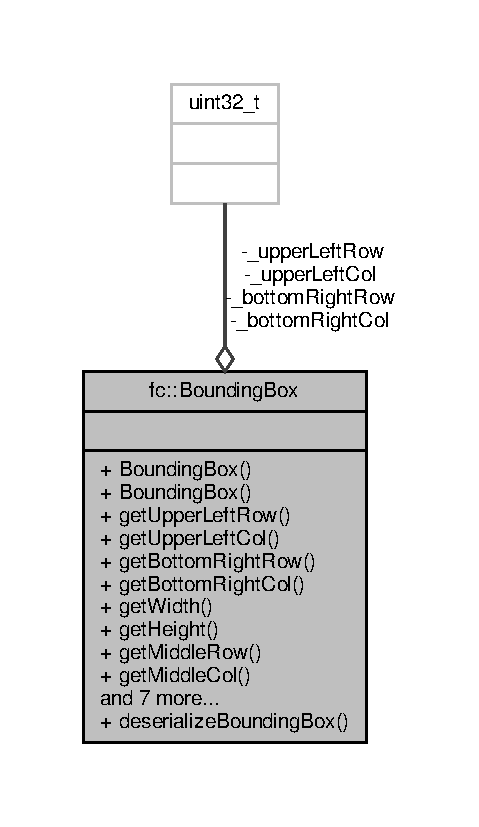
\includegraphics[width=230pt]{df/dd9/classfc_1_1BoundingBox__coll__graph}
\end{center}
\end{figure}
\subsection*{Public Member Functions}
\begin{DoxyCompactItemize}
\item 
\hyperlink{classfc_1_1BoundingBox_a521a34a72d4e4786d4c5e910b7334407}{Bounding\+Box} (uint32\+\_\+t upper\+Left\+Row, uint32\+\_\+t upper\+Left\+Col, uint32\+\_\+t bottom\+Right\+Row, uint32\+\_\+t bottom\+Right\+Col)
\begin{DoxyCompactList}\small\item\em Bounding box constructor. \end{DoxyCompactList}\item 
\hyperlink{classfc_1_1BoundingBox_aeb427ee69514165e4d4357a007c963c1}{Bounding\+Box} (const \hyperlink{classfc_1_1BoundingBox}{Bounding\+Box} \&src)
\begin{DoxyCompactList}\small\item\em Copy constructor. \end{DoxyCompactList}\item 
uint32\+\_\+t \hyperlink{classfc_1_1BoundingBox_a921418d145cc148a50d599b51447215a}{get\+Upper\+Left\+Row} () const
\begin{DoxyCompactList}\small\item\em Getter to the upper left row. \end{DoxyCompactList}\item 
uint32\+\_\+t \hyperlink{classfc_1_1BoundingBox_a21e8dcad0b3d37aa0a37c6dab4200974}{get\+Upper\+Left\+Col} () const
\begin{DoxyCompactList}\small\item\em Getter to the upper left column. \end{DoxyCompactList}\item 
uint32\+\_\+t \hyperlink{classfc_1_1BoundingBox_a74411180845c0572329c693170621245}{get\+Bottom\+Right\+Row} () const
\begin{DoxyCompactList}\small\item\em Getter to the bottom right row. \end{DoxyCompactList}\item 
uint32\+\_\+t \hyperlink{classfc_1_1BoundingBox_aedfb5b832d699a78a954c6778208414c}{get\+Bottom\+Right\+Col} () const
\begin{DoxyCompactList}\small\item\em Getter to the bottom right column. \end{DoxyCompactList}\item 
uint32\+\_\+t \hyperlink{classfc_1_1BoundingBox_aecdcbec558ef3396ed42924d4937d981}{get\+Width} () const
\begin{DoxyCompactList}\small\item\em Getter the Bounding Box width. \end{DoxyCompactList}\item 
uint32\+\_\+t \hyperlink{classfc_1_1BoundingBox_a9f26359f081940896dcf90ab5d5f0132}{get\+Height} () const
\begin{DoxyCompactList}\small\item\em Getter to the Bounding Box height. \end{DoxyCompactList}\item 
double \hyperlink{classfc_1_1BoundingBox_a96d9180aacc790de07f07dde841e9d01}{get\+Middle\+Row} () const
\begin{DoxyCompactList}\small\item\em Getter to the middle row. \end{DoxyCompactList}\item 
double \hyperlink{classfc_1_1BoundingBox_a5d829bb45a327c47b4a6d4f563cbef0c}{get\+Middle\+Col} () const
\begin{DoxyCompactList}\small\item\em Getter to the middle column. \end{DoxyCompactList}\item 
void \hyperlink{classfc_1_1BoundingBox_a8007ac29ae2e3f15bfccf71d6f318716}{set\+Upper\+Left\+Row} (uint32\+\_\+t row\+Top\+Left)
\begin{DoxyCompactList}\small\item\em Setter to the upper left row. \end{DoxyCompactList}\item 
void \hyperlink{classfc_1_1BoundingBox_aabde814367dcfa4d1f1e23042d655cc4}{set\+Upper\+Left\+Col} (uint32\+\_\+t col\+Top\+Left)
\begin{DoxyCompactList}\small\item\em Setter to the upper left column. \end{DoxyCompactList}\item 
void \hyperlink{classfc_1_1BoundingBox_a88812242713670dc43c3137b0a962cbe}{set\+Bottom\+Right\+Row} (uint32\+\_\+t bottom\+Right\+Row)
\begin{DoxyCompactList}\small\item\em Setter to the bottom right row. \end{DoxyCompactList}\item 
void \hyperlink{classfc_1_1BoundingBox_af24b7c088410245b0aa492cf0b200e2e}{set\+Bottom\+Right\+Col} (uint32\+\_\+t bottom\+Right\+Col)
\begin{DoxyCompactList}\small\item\em Setter to the bottom right column. \end{DoxyCompactList}\item 
void \hyperlink{classfc_1_1BoundingBox_ae2174abc444c26d86763567ed31c5094}{serialize\+Bounding\+Box} (std\+::ofstream \&out\+File)
\begin{DoxyCompactList}\small\item\em Serialize a Bounding box into a output stream. \end{DoxyCompactList}\item 
\hyperlink{classfc_1_1BoundingBox}{Bounding\+Box} \& \hyperlink{classfc_1_1BoundingBox_a80e775cb93499c77462ea281d9740f74}{operator=} (const \hyperlink{classfc_1_1BoundingBox}{Bounding\+Box} \&other)
\begin{DoxyCompactList}\small\item\em Assignement operator. \end{DoxyCompactList}\item 
bool \hyperlink{classfc_1_1BoundingBox_a2a1f28a0e0cd0a8b6041ba8e9c0f9b4f}{operator==} (const \hyperlink{classfc_1_1BoundingBox}{Bounding\+Box} \&bB) const
\begin{DoxyCompactList}\small\item\em Equality operator to test purpose. \end{DoxyCompactList}\end{DoxyCompactItemize}
\subsection*{Static Public Member Functions}
\begin{DoxyCompactItemize}
\item 
static \hyperlink{classfc_1_1BoundingBox}{Bounding\+Box} \hyperlink{classfc_1_1BoundingBox_acdd286d48651286d78c1b1eabe2357c9}{deserialize\+Bounding\+Box} (std\+::ifstream \&in\+File)
\begin{DoxyCompactList}\small\item\em Deserialize a bounding box from a file. \end{DoxyCompactList}\end{DoxyCompactItemize}
\subsection*{Private Attributes}
\begin{DoxyCompactItemize}
\item 
uint32\+\_\+t \hyperlink{classfc_1_1BoundingBox_a9e75c4e7a1249bfd286d3c2cdb8bce84}{\+\_\+upper\+Left\+Row}
\begin{DoxyCompactList}\small\item\em Bounding box upper left row. \end{DoxyCompactList}\item 
uint32\+\_\+t \hyperlink{classfc_1_1BoundingBox_a5e384b0edc1e5ae8c264c74f317725ea}{\+\_\+upper\+Left\+Col}
\begin{DoxyCompactList}\small\item\em Bounding box upper left col. \end{DoxyCompactList}\item 
uint32\+\_\+t \hyperlink{classfc_1_1BoundingBox_a9797ed1e8272f512abd7b2c0598766e5}{\+\_\+bottom\+Right\+Row}
\begin{DoxyCompactList}\small\item\em Bounding box bottom right row. \end{DoxyCompactList}\item 
uint32\+\_\+t \hyperlink{classfc_1_1BoundingBox_a1ac6bfcd930956a8cf7e580b83e88147}{\+\_\+bottom\+Right\+Col}
\begin{DoxyCompactList}\small\item\em Bounding box bottom right col. \end{DoxyCompactList}\end{DoxyCompactItemize}
\subsection*{Friends}
\begin{DoxyCompactItemize}
\item 
std\+::ostream \& \hyperlink{classfc_1_1BoundingBox_a9b77edf50fd5d4a4bd03dda7eb3054fe}{operator$<$$<$} (std\+::ostream \&os, const \hyperlink{classfc_1_1BoundingBox}{Bounding\+Box} \&box)
\begin{DoxyCompactList}\small\item\em Bounding box output stream operator. \end{DoxyCompactList}\end{DoxyCompactItemize}


\subsection{Detailed Description}
Define a bounding box around a feature. 

Definition at line 48 of file Bounding\+Box.\+h.



\subsection{Constructor \& Destructor Documentation}
\mbox{\Hypertarget{classfc_1_1BoundingBox_a521a34a72d4e4786d4c5e910b7334407}\label{classfc_1_1BoundingBox_a521a34a72d4e4786d4c5e910b7334407}} 
\index{fc\+::\+Bounding\+Box@{fc\+::\+Bounding\+Box}!Bounding\+Box@{Bounding\+Box}}
\index{Bounding\+Box@{Bounding\+Box}!fc\+::\+Bounding\+Box@{fc\+::\+Bounding\+Box}}
\subsubsection{\texorpdfstring{Bounding\+Box()}{BoundingBox()}\hspace{0.1cm}{\footnotesize\ttfamily [1/2]}}
{\footnotesize\ttfamily fc\+::\+Bounding\+Box\+::\+Bounding\+Box (\begin{DoxyParamCaption}\item[{uint32\+\_\+t}]{upper\+Left\+Row,  }\item[{uint32\+\_\+t}]{upper\+Left\+Col,  }\item[{uint32\+\_\+t}]{bottom\+Right\+Row,  }\item[{uint32\+\_\+t}]{bottom\+Right\+Col }\end{DoxyParamCaption})\hspace{0.3cm}{\ttfamily [inline]}, {\ttfamily [explicit]}}



Bounding box constructor. 


\begin{DoxyParams}{Parameters}
{\em upper\+Left\+Row} & Upper left row in global coordinate \\
\hline
{\em upper\+Left\+Col} & Upper left column in global coordinate \\
\hline
{\em bottom\+Right\+Row} & Bottom right row in global coordinate \\
\hline
{\em bottom\+Right\+Col} & Bottom right column in global coordinate \\
\hline
\end{DoxyParams}


Definition at line 55 of file Bounding\+Box.\+h.

Here is the caller graph for this function\+:
\nopagebreak
\begin{figure}[H]
\begin{center}
\leavevmode
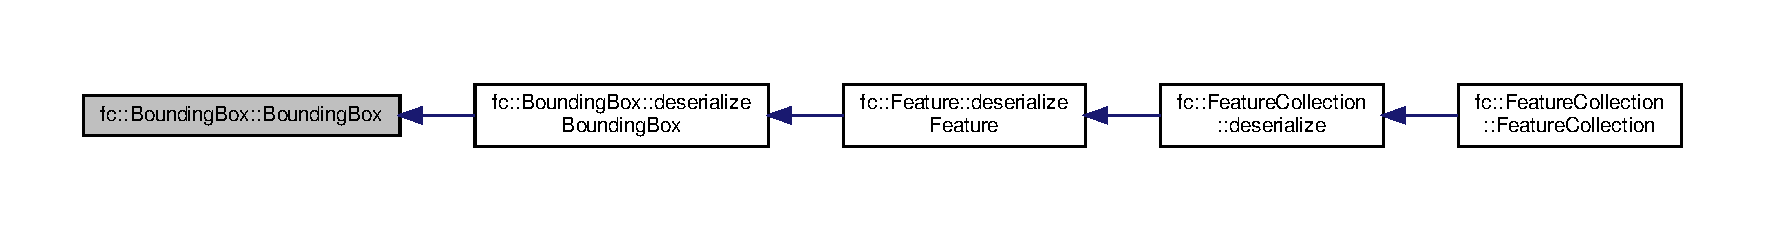
\includegraphics[width=350pt]{db/dc1/classfc_1_1BoundingBox_a521a34a72d4e4786d4c5e910b7334407_icgraph}
\end{center}
\end{figure}
\mbox{\Hypertarget{classfc_1_1BoundingBox_aeb427ee69514165e4d4357a007c963c1}\label{classfc_1_1BoundingBox_aeb427ee69514165e4d4357a007c963c1}} 
\index{fc\+::\+Bounding\+Box@{fc\+::\+Bounding\+Box}!Bounding\+Box@{Bounding\+Box}}
\index{Bounding\+Box@{Bounding\+Box}!fc\+::\+Bounding\+Box@{fc\+::\+Bounding\+Box}}
\subsubsection{\texorpdfstring{Bounding\+Box()}{BoundingBox()}\hspace{0.1cm}{\footnotesize\ttfamily [2/2]}}
{\footnotesize\ttfamily fc\+::\+Bounding\+Box\+::\+Bounding\+Box (\begin{DoxyParamCaption}\item[{const \hyperlink{classfc_1_1BoundingBox}{Bounding\+Box} \&}]{src }\end{DoxyParamCaption})\hspace{0.3cm}{\ttfamily [inline]}}



Copy constructor. 


\begin{DoxyParams}{Parameters}
{\em src} & Bounding box to copy \\
\hline
\end{DoxyParams}


Definition at line 64 of file Bounding\+Box.\+h.

Here is the call graph for this function\+:
\nopagebreak
\begin{figure}[H]
\begin{center}
\leavevmode
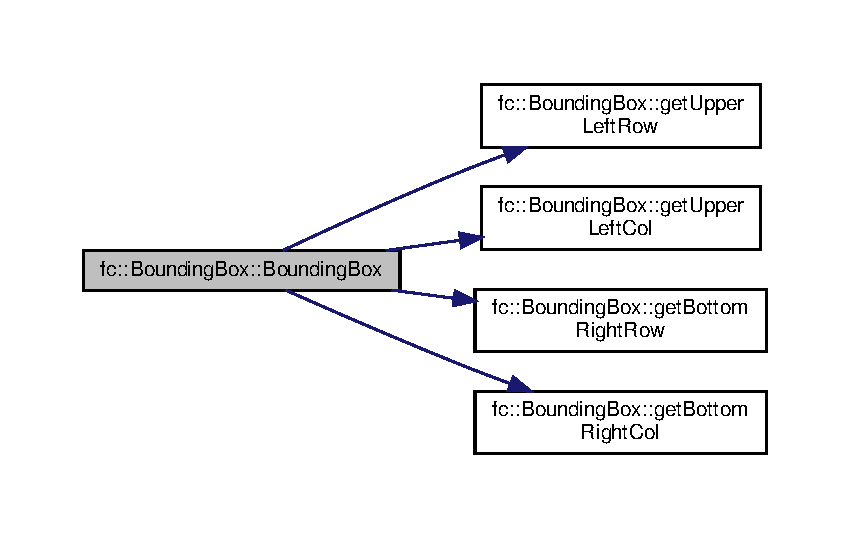
\includegraphics[width=350pt]{db/dc1/classfc_1_1BoundingBox_aeb427ee69514165e4d4357a007c963c1_cgraph}
\end{center}
\end{figure}


\subsection{Member Function Documentation}
\mbox{\Hypertarget{classfc_1_1BoundingBox_acdd286d48651286d78c1b1eabe2357c9}\label{classfc_1_1BoundingBox_acdd286d48651286d78c1b1eabe2357c9}} 
\index{fc\+::\+Bounding\+Box@{fc\+::\+Bounding\+Box}!deserialize\+Bounding\+Box@{deserialize\+Bounding\+Box}}
\index{deserialize\+Bounding\+Box@{deserialize\+Bounding\+Box}!fc\+::\+Bounding\+Box@{fc\+::\+Bounding\+Box}}
\subsubsection{\texorpdfstring{deserialize\+Bounding\+Box()}{deserializeBoundingBox()}}
{\footnotesize\ttfamily static \hyperlink{classfc_1_1BoundingBox}{Bounding\+Box} fc\+::\+Bounding\+Box\+::deserialize\+Bounding\+Box (\begin{DoxyParamCaption}\item[{std\+::ifstream \&}]{in\+File }\end{DoxyParamCaption})\hspace{0.3cm}{\ttfamily [inline]}, {\ttfamily [static]}}



Deserialize a bounding box from a file. 


\begin{DoxyParams}{Parameters}
{\em in\+File} & File to deserialized \\
\hline
\end{DoxyParams}
\begin{DoxyReturn}{Returns}
Bounding box deserialized from the input file 
\end{DoxyReturn}


Definition at line 139 of file Bounding\+Box.\+h.

Here is the call graph for this function\+:
\nopagebreak
\begin{figure}[H]
\begin{center}
\leavevmode
\includegraphics[width=350pt]{db/dc1/classfc_1_1BoundingBox_acdd286d48651286d78c1b1eabe2357c9_cgraph}
\end{center}
\end{figure}
Here is the caller graph for this function\+:
\nopagebreak
\begin{figure}[H]
\begin{center}
\leavevmode
\includegraphics[width=350pt]{db/dc1/classfc_1_1BoundingBox_acdd286d48651286d78c1b1eabe2357c9_icgraph}
\end{center}
\end{figure}
\mbox{\Hypertarget{classfc_1_1BoundingBox_aedfb5b832d699a78a954c6778208414c}\label{classfc_1_1BoundingBox_aedfb5b832d699a78a954c6778208414c}} 
\index{fc\+::\+Bounding\+Box@{fc\+::\+Bounding\+Box}!get\+Bottom\+Right\+Col@{get\+Bottom\+Right\+Col}}
\index{get\+Bottom\+Right\+Col@{get\+Bottom\+Right\+Col}!fc\+::\+Bounding\+Box@{fc\+::\+Bounding\+Box}}
\subsubsection{\texorpdfstring{get\+Bottom\+Right\+Col()}{getBottomRightCol()}}
{\footnotesize\ttfamily uint32\+\_\+t fc\+::\+Bounding\+Box\+::get\+Bottom\+Right\+Col (\begin{DoxyParamCaption}{ }\end{DoxyParamCaption}) const\hspace{0.3cm}{\ttfamily [inline]}}



Getter to the bottom right column. 

\begin{DoxyReturn}{Returns}
The bottom right column 
\end{DoxyReturn}


Definition at line 85 of file Bounding\+Box.\+h.

Here is the caller graph for this function\+:
\nopagebreak
\begin{figure}[H]
\begin{center}
\leavevmode
\includegraphics[width=350pt]{db/dc1/classfc_1_1BoundingBox_aedfb5b832d699a78a954c6778208414c_icgraph}
\end{center}
\end{figure}
\mbox{\Hypertarget{classfc_1_1BoundingBox_a74411180845c0572329c693170621245}\label{classfc_1_1BoundingBox_a74411180845c0572329c693170621245}} 
\index{fc\+::\+Bounding\+Box@{fc\+::\+Bounding\+Box}!get\+Bottom\+Right\+Row@{get\+Bottom\+Right\+Row}}
\index{get\+Bottom\+Right\+Row@{get\+Bottom\+Right\+Row}!fc\+::\+Bounding\+Box@{fc\+::\+Bounding\+Box}}
\subsubsection{\texorpdfstring{get\+Bottom\+Right\+Row()}{getBottomRightRow()}}
{\footnotesize\ttfamily uint32\+\_\+t fc\+::\+Bounding\+Box\+::get\+Bottom\+Right\+Row (\begin{DoxyParamCaption}{ }\end{DoxyParamCaption}) const\hspace{0.3cm}{\ttfamily [inline]}}



Getter to the bottom right row. 

\begin{DoxyReturn}{Returns}
The bottom right row 
\end{DoxyReturn}


Definition at line 81 of file Bounding\+Box.\+h.

Here is the caller graph for this function\+:
\nopagebreak
\begin{figure}[H]
\begin{center}
\leavevmode
\includegraphics[width=350pt]{db/dc1/classfc_1_1BoundingBox_a74411180845c0572329c693170621245_icgraph}
\end{center}
\end{figure}
\mbox{\Hypertarget{classfc_1_1BoundingBox_a9f26359f081940896dcf90ab5d5f0132}\label{classfc_1_1BoundingBox_a9f26359f081940896dcf90ab5d5f0132}} 
\index{fc\+::\+Bounding\+Box@{fc\+::\+Bounding\+Box}!get\+Height@{get\+Height}}
\index{get\+Height@{get\+Height}!fc\+::\+Bounding\+Box@{fc\+::\+Bounding\+Box}}
\subsubsection{\texorpdfstring{get\+Height()}{getHeight()}}
{\footnotesize\ttfamily uint32\+\_\+t fc\+::\+Bounding\+Box\+::get\+Height (\begin{DoxyParamCaption}{ }\end{DoxyParamCaption}) const\hspace{0.3cm}{\ttfamily [inline]}}



Getter to the Bounding Box height. 

\begin{DoxyReturn}{Returns}
The Bounding Box height 
\end{DoxyReturn}


Definition at line 93 of file Bounding\+Box.\+h.

Here is the caller graph for this function\+:
\nopagebreak
\begin{figure}[H]
\begin{center}
\leavevmode
\includegraphics[width=350pt]{db/dc1/classfc_1_1BoundingBox_a9f26359f081940896dcf90ab5d5f0132_icgraph}
\end{center}
\end{figure}
\mbox{\Hypertarget{classfc_1_1BoundingBox_a5d829bb45a327c47b4a6d4f563cbef0c}\label{classfc_1_1BoundingBox_a5d829bb45a327c47b4a6d4f563cbef0c}} 
\index{fc\+::\+Bounding\+Box@{fc\+::\+Bounding\+Box}!get\+Middle\+Col@{get\+Middle\+Col}}
\index{get\+Middle\+Col@{get\+Middle\+Col}!fc\+::\+Bounding\+Box@{fc\+::\+Bounding\+Box}}
\subsubsection{\texorpdfstring{get\+Middle\+Col()}{getMiddleCol()}}
{\footnotesize\ttfamily double fc\+::\+Bounding\+Box\+::get\+Middle\+Col (\begin{DoxyParamCaption}{ }\end{DoxyParamCaption}) const\hspace{0.3cm}{\ttfamily [inline]}}



Getter to the middle column. 

\begin{DoxyReturn}{Returns}
The middle column 
\end{DoxyReturn}


Definition at line 103 of file Bounding\+Box.\+h.

Here is the caller graph for this function\+:
\nopagebreak
\begin{figure}[H]
\begin{center}
\leavevmode
\includegraphics[width=350pt]{db/dc1/classfc_1_1BoundingBox_a5d829bb45a327c47b4a6d4f563cbef0c_icgraph}
\end{center}
\end{figure}
\mbox{\Hypertarget{classfc_1_1BoundingBox_a96d9180aacc790de07f07dde841e9d01}\label{classfc_1_1BoundingBox_a96d9180aacc790de07f07dde841e9d01}} 
\index{fc\+::\+Bounding\+Box@{fc\+::\+Bounding\+Box}!get\+Middle\+Row@{get\+Middle\+Row}}
\index{get\+Middle\+Row@{get\+Middle\+Row}!fc\+::\+Bounding\+Box@{fc\+::\+Bounding\+Box}}
\subsubsection{\texorpdfstring{get\+Middle\+Row()}{getMiddleRow()}}
{\footnotesize\ttfamily double fc\+::\+Bounding\+Box\+::get\+Middle\+Row (\begin{DoxyParamCaption}{ }\end{DoxyParamCaption}) const\hspace{0.3cm}{\ttfamily [inline]}}



Getter to the middle row. 

\begin{DoxyReturn}{Returns}
The middle row 
\end{DoxyReturn}


Definition at line 97 of file Bounding\+Box.\+h.

Here is the caller graph for this function\+:
\nopagebreak
\begin{figure}[H]
\begin{center}
\leavevmode
\includegraphics[width=350pt]{db/dc1/classfc_1_1BoundingBox_a96d9180aacc790de07f07dde841e9d01_icgraph}
\end{center}
\end{figure}
\mbox{\Hypertarget{classfc_1_1BoundingBox_a21e8dcad0b3d37aa0a37c6dab4200974}\label{classfc_1_1BoundingBox_a21e8dcad0b3d37aa0a37c6dab4200974}} 
\index{fc\+::\+Bounding\+Box@{fc\+::\+Bounding\+Box}!get\+Upper\+Left\+Col@{get\+Upper\+Left\+Col}}
\index{get\+Upper\+Left\+Col@{get\+Upper\+Left\+Col}!fc\+::\+Bounding\+Box@{fc\+::\+Bounding\+Box}}
\subsubsection{\texorpdfstring{get\+Upper\+Left\+Col()}{getUpperLeftCol()}}
{\footnotesize\ttfamily uint32\+\_\+t fc\+::\+Bounding\+Box\+::get\+Upper\+Left\+Col (\begin{DoxyParamCaption}{ }\end{DoxyParamCaption}) const\hspace{0.3cm}{\ttfamily [inline]}}



Getter to the upper left column. 

\begin{DoxyReturn}{Returns}
The upper left column 
\end{DoxyReturn}


Definition at line 77 of file Bounding\+Box.\+h.

Here is the caller graph for this function\+:
\nopagebreak
\begin{figure}[H]
\begin{center}
\leavevmode
\includegraphics[width=350pt]{db/dc1/classfc_1_1BoundingBox_a21e8dcad0b3d37aa0a37c6dab4200974_icgraph}
\end{center}
\end{figure}
\mbox{\Hypertarget{classfc_1_1BoundingBox_a921418d145cc148a50d599b51447215a}\label{classfc_1_1BoundingBox_a921418d145cc148a50d599b51447215a}} 
\index{fc\+::\+Bounding\+Box@{fc\+::\+Bounding\+Box}!get\+Upper\+Left\+Row@{get\+Upper\+Left\+Row}}
\index{get\+Upper\+Left\+Row@{get\+Upper\+Left\+Row}!fc\+::\+Bounding\+Box@{fc\+::\+Bounding\+Box}}
\subsubsection{\texorpdfstring{get\+Upper\+Left\+Row()}{getUpperLeftRow()}}
{\footnotesize\ttfamily uint32\+\_\+t fc\+::\+Bounding\+Box\+::get\+Upper\+Left\+Row (\begin{DoxyParamCaption}{ }\end{DoxyParamCaption}) const\hspace{0.3cm}{\ttfamily [inline]}}



Getter to the upper left row. 

\begin{DoxyReturn}{Returns}
The upper left row 
\end{DoxyReturn}


Definition at line 73 of file Bounding\+Box.\+h.

Here is the caller graph for this function\+:
\nopagebreak
\begin{figure}[H]
\begin{center}
\leavevmode
\includegraphics[width=350pt]{db/dc1/classfc_1_1BoundingBox_a921418d145cc148a50d599b51447215a_icgraph}
\end{center}
\end{figure}
\mbox{\Hypertarget{classfc_1_1BoundingBox_aecdcbec558ef3396ed42924d4937d981}\label{classfc_1_1BoundingBox_aecdcbec558ef3396ed42924d4937d981}} 
\index{fc\+::\+Bounding\+Box@{fc\+::\+Bounding\+Box}!get\+Width@{get\+Width}}
\index{get\+Width@{get\+Width}!fc\+::\+Bounding\+Box@{fc\+::\+Bounding\+Box}}
\subsubsection{\texorpdfstring{get\+Width()}{getWidth()}}
{\footnotesize\ttfamily uint32\+\_\+t fc\+::\+Bounding\+Box\+::get\+Width (\begin{DoxyParamCaption}{ }\end{DoxyParamCaption}) const\hspace{0.3cm}{\ttfamily [inline]}}



Getter the Bounding Box width. 

\begin{DoxyReturn}{Returns}
The Bounding Box width 
\end{DoxyReturn}


Definition at line 89 of file Bounding\+Box.\+h.

Here is the caller graph for this function\+:
\nopagebreak
\begin{figure}[H]
\begin{center}
\leavevmode
\includegraphics[width=350pt]{db/dc1/classfc_1_1BoundingBox_aecdcbec558ef3396ed42924d4937d981_icgraph}
\end{center}
\end{figure}
\mbox{\Hypertarget{classfc_1_1BoundingBox_a80e775cb93499c77462ea281d9740f74}\label{classfc_1_1BoundingBox_a80e775cb93499c77462ea281d9740f74}} 
\index{fc\+::\+Bounding\+Box@{fc\+::\+Bounding\+Box}!operator=@{operator=}}
\index{operator=@{operator=}!fc\+::\+Bounding\+Box@{fc\+::\+Bounding\+Box}}
\subsubsection{\texorpdfstring{operator=()}{operator=()}}
{\footnotesize\ttfamily \hyperlink{classfc_1_1BoundingBox}{Bounding\+Box}\& fc\+::\+Bounding\+Box\+::operator= (\begin{DoxyParamCaption}\item[{const \hyperlink{classfc_1_1BoundingBox}{Bounding\+Box} \&}]{other }\end{DoxyParamCaption})\hspace{0.3cm}{\ttfamily [inline]}}



Assignement operator. 


\begin{DoxyParams}{Parameters}
{\em other} & Bounding box to copy \\
\hline
\end{DoxyParams}
\begin{DoxyReturn}{Returns}
Reference to the copied Bounding box 
\end{DoxyReturn}


Definition at line 160 of file Bounding\+Box.\+h.

Here is the call graph for this function\+:
\nopagebreak
\begin{figure}[H]
\begin{center}
\leavevmode
\includegraphics[width=350pt]{db/dc1/classfc_1_1BoundingBox_a80e775cb93499c77462ea281d9740f74_cgraph}
\end{center}
\end{figure}
\mbox{\Hypertarget{classfc_1_1BoundingBox_a2a1f28a0e0cd0a8b6041ba8e9c0f9b4f}\label{classfc_1_1BoundingBox_a2a1f28a0e0cd0a8b6041ba8e9c0f9b4f}} 
\index{fc\+::\+Bounding\+Box@{fc\+::\+Bounding\+Box}!operator==@{operator==}}
\index{operator==@{operator==}!fc\+::\+Bounding\+Box@{fc\+::\+Bounding\+Box}}
\subsubsection{\texorpdfstring{operator==()}{operator==()}}
{\footnotesize\ttfamily bool fc\+::\+Bounding\+Box\+::operator== (\begin{DoxyParamCaption}\item[{const \hyperlink{classfc_1_1BoundingBox}{Bounding\+Box} \&}]{bB }\end{DoxyParamCaption}) const\hspace{0.3cm}{\ttfamily [inline]}}



Equality operator to test purpose. 


\begin{DoxyParams}{Parameters}
{\em bB} & Bounding box to compare with \\
\hline
\end{DoxyParams}
\begin{DoxyReturn}{Returns}
True is the bounding box are equal, else False 
\end{DoxyReturn}


Definition at line 187 of file Bounding\+Box.\+h.

Here is the call graph for this function\+:
\nopagebreak
\begin{figure}[H]
\begin{center}
\leavevmode
\includegraphics[width=350pt]{db/dc1/classfc_1_1BoundingBox_a2a1f28a0e0cd0a8b6041ba8e9c0f9b4f_cgraph}
\end{center}
\end{figure}
\mbox{\Hypertarget{classfc_1_1BoundingBox_ae2174abc444c26d86763567ed31c5094}\label{classfc_1_1BoundingBox_ae2174abc444c26d86763567ed31c5094}} 
\index{fc\+::\+Bounding\+Box@{fc\+::\+Bounding\+Box}!serialize\+Bounding\+Box@{serialize\+Bounding\+Box}}
\index{serialize\+Bounding\+Box@{serialize\+Bounding\+Box}!fc\+::\+Bounding\+Box@{fc\+::\+Bounding\+Box}}
\subsubsection{\texorpdfstring{serialize\+Bounding\+Box()}{serializeBoundingBox()}}
{\footnotesize\ttfamily void fc\+::\+Bounding\+Box\+::serialize\+Bounding\+Box (\begin{DoxyParamCaption}\item[{std\+::ofstream \&}]{out\+File }\end{DoxyParamCaption})\hspace{0.3cm}{\ttfamily [inline]}}



Serialize a Bounding box into a output stream. 


\begin{DoxyParams}{Parameters}
{\em out\+File} & output stream to put the bounding box serial \\
\hline
\end{DoxyParams}


Definition at line 129 of file Bounding\+Box.\+h.

Here is the caller graph for this function\+:
\nopagebreak
\begin{figure}[H]
\begin{center}
\leavevmode
\includegraphics[width=350pt]{db/dc1/classfc_1_1BoundingBox_ae2174abc444c26d86763567ed31c5094_icgraph}
\end{center}
\end{figure}
\mbox{\Hypertarget{classfc_1_1BoundingBox_af24b7c088410245b0aa492cf0b200e2e}\label{classfc_1_1BoundingBox_af24b7c088410245b0aa492cf0b200e2e}} 
\index{fc\+::\+Bounding\+Box@{fc\+::\+Bounding\+Box}!set\+Bottom\+Right\+Col@{set\+Bottom\+Right\+Col}}
\index{set\+Bottom\+Right\+Col@{set\+Bottom\+Right\+Col}!fc\+::\+Bounding\+Box@{fc\+::\+Bounding\+Box}}
\subsubsection{\texorpdfstring{set\+Bottom\+Right\+Col()}{setBottomRightCol()}}
{\footnotesize\ttfamily void fc\+::\+Bounding\+Box\+::set\+Bottom\+Right\+Col (\begin{DoxyParamCaption}\item[{uint32\+\_\+t}]{bottom\+Right\+Col }\end{DoxyParamCaption})\hspace{0.3cm}{\ttfamily [inline]}}



Setter to the bottom right column. 


\begin{DoxyParams}{Parameters}
{\em bottom\+Right\+Col} & Bottom right column to set \\
\hline
\end{DoxyParams}


Definition at line 123 of file Bounding\+Box.\+h.

Here is the caller graph for this function\+:
\nopagebreak
\begin{figure}[H]
\begin{center}
\leavevmode
\includegraphics[width=350pt]{db/dc1/classfc_1_1BoundingBox_af24b7c088410245b0aa492cf0b200e2e_icgraph}
\end{center}
\end{figure}
\mbox{\Hypertarget{classfc_1_1BoundingBox_a88812242713670dc43c3137b0a962cbe}\label{classfc_1_1BoundingBox_a88812242713670dc43c3137b0a962cbe}} 
\index{fc\+::\+Bounding\+Box@{fc\+::\+Bounding\+Box}!set\+Bottom\+Right\+Row@{set\+Bottom\+Right\+Row}}
\index{set\+Bottom\+Right\+Row@{set\+Bottom\+Right\+Row}!fc\+::\+Bounding\+Box@{fc\+::\+Bounding\+Box}}
\subsubsection{\texorpdfstring{set\+Bottom\+Right\+Row()}{setBottomRightRow()}}
{\footnotesize\ttfamily void fc\+::\+Bounding\+Box\+::set\+Bottom\+Right\+Row (\begin{DoxyParamCaption}\item[{uint32\+\_\+t}]{bottom\+Right\+Row }\end{DoxyParamCaption})\hspace{0.3cm}{\ttfamily [inline]}}



Setter to the bottom right row. 


\begin{DoxyParams}{Parameters}
{\em bottom\+Right\+Row} & Bottom right row to set \\
\hline
\end{DoxyParams}


Definition at line 117 of file Bounding\+Box.\+h.

Here is the caller graph for this function\+:
\nopagebreak
\begin{figure}[H]
\begin{center}
\leavevmode
\includegraphics[width=350pt]{db/dc1/classfc_1_1BoundingBox_a88812242713670dc43c3137b0a962cbe_icgraph}
\end{center}
\end{figure}
\mbox{\Hypertarget{classfc_1_1BoundingBox_aabde814367dcfa4d1f1e23042d655cc4}\label{classfc_1_1BoundingBox_aabde814367dcfa4d1f1e23042d655cc4}} 
\index{fc\+::\+Bounding\+Box@{fc\+::\+Bounding\+Box}!set\+Upper\+Left\+Col@{set\+Upper\+Left\+Col}}
\index{set\+Upper\+Left\+Col@{set\+Upper\+Left\+Col}!fc\+::\+Bounding\+Box@{fc\+::\+Bounding\+Box}}
\subsubsection{\texorpdfstring{set\+Upper\+Left\+Col()}{setUpperLeftCol()}}
{\footnotesize\ttfamily void fc\+::\+Bounding\+Box\+::set\+Upper\+Left\+Col (\begin{DoxyParamCaption}\item[{uint32\+\_\+t}]{col\+Top\+Left }\end{DoxyParamCaption})\hspace{0.3cm}{\ttfamily [inline]}}



Setter to the upper left column. 


\begin{DoxyParams}{Parameters}
{\em col\+Top\+Left} & The upper left column to set \\
\hline
\end{DoxyParams}


Definition at line 113 of file Bounding\+Box.\+h.

Here is the caller graph for this function\+:
\nopagebreak
\begin{figure}[H]
\begin{center}
\leavevmode
\includegraphics[width=350pt]{db/dc1/classfc_1_1BoundingBox_aabde814367dcfa4d1f1e23042d655cc4_icgraph}
\end{center}
\end{figure}
\mbox{\Hypertarget{classfc_1_1BoundingBox_a8007ac29ae2e3f15bfccf71d6f318716}\label{classfc_1_1BoundingBox_a8007ac29ae2e3f15bfccf71d6f318716}} 
\index{fc\+::\+Bounding\+Box@{fc\+::\+Bounding\+Box}!set\+Upper\+Left\+Row@{set\+Upper\+Left\+Row}}
\index{set\+Upper\+Left\+Row@{set\+Upper\+Left\+Row}!fc\+::\+Bounding\+Box@{fc\+::\+Bounding\+Box}}
\subsubsection{\texorpdfstring{set\+Upper\+Left\+Row()}{setUpperLeftRow()}}
{\footnotesize\ttfamily void fc\+::\+Bounding\+Box\+::set\+Upper\+Left\+Row (\begin{DoxyParamCaption}\item[{uint32\+\_\+t}]{row\+Top\+Left }\end{DoxyParamCaption})\hspace{0.3cm}{\ttfamily [inline]}}



Setter to the upper left row. 


\begin{DoxyParams}{Parameters}
{\em row\+Top\+Left} & To the upper left row to set \\
\hline
\end{DoxyParams}


Definition at line 109 of file Bounding\+Box.\+h.

Here is the caller graph for this function\+:
\nopagebreak
\begin{figure}[H]
\begin{center}
\leavevmode
\includegraphics[width=350pt]{db/dc1/classfc_1_1BoundingBox_a8007ac29ae2e3f15bfccf71d6f318716_icgraph}
\end{center}
\end{figure}


\subsection{Friends And Related Function Documentation}
\mbox{\Hypertarget{classfc_1_1BoundingBox_a9b77edf50fd5d4a4bd03dda7eb3054fe}\label{classfc_1_1BoundingBox_a9b77edf50fd5d4a4bd03dda7eb3054fe}} 
\index{fc\+::\+Bounding\+Box@{fc\+::\+Bounding\+Box}!operator$<$$<$@{operator$<$$<$}}
\index{operator$<$$<$@{operator$<$$<$}!fc\+::\+Bounding\+Box@{fc\+::\+Bounding\+Box}}
\subsubsection{\texorpdfstring{operator$<$$<$}{operator<<}}
{\footnotesize\ttfamily std\+::ostream\& operator$<$$<$ (\begin{DoxyParamCaption}\item[{std\+::ostream \&}]{os,  }\item[{const \hyperlink{classfc_1_1BoundingBox}{Bounding\+Box} \&}]{box }\end{DoxyParamCaption})\hspace{0.3cm}{\ttfamily [friend]}}



Bounding box output stream operator. 


\begin{DoxyParams}{Parameters}
{\em os} & Output stream \\
\hline
{\em box} & Bounding box to print \\
\hline
\end{DoxyParams}
\begin{DoxyReturn}{Returns}
Output stream with the data printed 
\end{DoxyReturn}


Definition at line 174 of file Bounding\+Box.\+h.



\subsection{Member Data Documentation}
\mbox{\Hypertarget{classfc_1_1BoundingBox_a1ac6bfcd930956a8cf7e580b83e88147}\label{classfc_1_1BoundingBox_a1ac6bfcd930956a8cf7e580b83e88147}} 
\index{fc\+::\+Bounding\+Box@{fc\+::\+Bounding\+Box}!\+\_\+bottom\+Right\+Col@{\+\_\+bottom\+Right\+Col}}
\index{\+\_\+bottom\+Right\+Col@{\+\_\+bottom\+Right\+Col}!fc\+::\+Bounding\+Box@{fc\+::\+Bounding\+Box}}
\subsubsection{\texorpdfstring{\+\_\+bottom\+Right\+Col}{\_bottomRightCol}}
{\footnotesize\ttfamily uint32\+\_\+t fc\+::\+Bounding\+Box\+::\+\_\+bottom\+Right\+Col\hspace{0.3cm}{\ttfamily [private]}}



Bounding box bottom right col. 



Definition at line 197 of file Bounding\+Box.\+h.

\mbox{\Hypertarget{classfc_1_1BoundingBox_a9797ed1e8272f512abd7b2c0598766e5}\label{classfc_1_1BoundingBox_a9797ed1e8272f512abd7b2c0598766e5}} 
\index{fc\+::\+Bounding\+Box@{fc\+::\+Bounding\+Box}!\+\_\+bottom\+Right\+Row@{\+\_\+bottom\+Right\+Row}}
\index{\+\_\+bottom\+Right\+Row@{\+\_\+bottom\+Right\+Row}!fc\+::\+Bounding\+Box@{fc\+::\+Bounding\+Box}}
\subsubsection{\texorpdfstring{\+\_\+bottom\+Right\+Row}{\_bottomRightRow}}
{\footnotesize\ttfamily uint32\+\_\+t fc\+::\+Bounding\+Box\+::\+\_\+bottom\+Right\+Row\hspace{0.3cm}{\ttfamily [private]}}



Bounding box bottom right row. 



Definition at line 197 of file Bounding\+Box.\+h.

\mbox{\Hypertarget{classfc_1_1BoundingBox_a5e384b0edc1e5ae8c264c74f317725ea}\label{classfc_1_1BoundingBox_a5e384b0edc1e5ae8c264c74f317725ea}} 
\index{fc\+::\+Bounding\+Box@{fc\+::\+Bounding\+Box}!\+\_\+upper\+Left\+Col@{\+\_\+upper\+Left\+Col}}
\index{\+\_\+upper\+Left\+Col@{\+\_\+upper\+Left\+Col}!fc\+::\+Bounding\+Box@{fc\+::\+Bounding\+Box}}
\subsubsection{\texorpdfstring{\+\_\+upper\+Left\+Col}{\_upperLeftCol}}
{\footnotesize\ttfamily uint32\+\_\+t fc\+::\+Bounding\+Box\+::\+\_\+upper\+Left\+Col\hspace{0.3cm}{\ttfamily [private]}}



Bounding box upper left col. 



Definition at line 197 of file Bounding\+Box.\+h.

\mbox{\Hypertarget{classfc_1_1BoundingBox_a9e75c4e7a1249bfd286d3c2cdb8bce84}\label{classfc_1_1BoundingBox_a9e75c4e7a1249bfd286d3c2cdb8bce84}} 
\index{fc\+::\+Bounding\+Box@{fc\+::\+Bounding\+Box}!\+\_\+upper\+Left\+Row@{\+\_\+upper\+Left\+Row}}
\index{\+\_\+upper\+Left\+Row@{\+\_\+upper\+Left\+Row}!fc\+::\+Bounding\+Box@{fc\+::\+Bounding\+Box}}
\subsubsection{\texorpdfstring{\+\_\+upper\+Left\+Row}{\_upperLeftRow}}
{\footnotesize\ttfamily uint32\+\_\+t fc\+::\+Bounding\+Box\+::\+\_\+upper\+Left\+Row\hspace{0.3cm}{\ttfamily [private]}}



Bounding box upper left row. 



Definition at line 197 of file Bounding\+Box.\+h.



The documentation for this class was generated from the following file\+:\begin{DoxyCompactItemize}
\item 
/home/anb22/\+Documents/\+Fast-\/\+Image/\+Fast\+Image/src/\+Fast\+Image/\+Feature\+Collection/\hyperlink{BoundingBox_8h}{Bounding\+Box.\+h}\end{DoxyCompactItemize}

\hypertarget{classfi_1_1CachedTile}{}\section{fi\+:\+:Cached\+Tile$<$ User\+Type $>$ Class Template Reference}
\label{classfi_1_1CachedTile}\index{fi\+::\+Cached\+Tile$<$ User\+Type $>$@{fi\+::\+Cached\+Tile$<$ User\+Type $>$}}


Tile Cached from the file.  




{\ttfamily \#include $<$Fast\+Image/data/\+Cached\+Tile.\+h$>$}



Collaboration diagram for fi\+:\+:Cached\+Tile$<$ User\+Type $>$\+:
\nopagebreak
\begin{figure}[H]
\begin{center}
\leavevmode
\includegraphics[width=350pt]{d5/da1/classfi_1_1CachedTile__coll__graph}
\end{center}
\end{figure}
\subsection*{Public Member Functions}
\begin{DoxyCompactItemize}
\item 
\hyperlink{classfi_1_1CachedTile_a1dd05836168d06224fd540d576e4e6e2}{Cached\+Tile} (uint32\+\_\+t tile\+Width, uint32\+\_\+t tile\+Height)
\begin{DoxyCompactList}\small\item\em \hyperlink{classfi_1_1CachedTile}{Cached\+Tile} Constructor, allocate the data buffer. \end{DoxyCompactList}\item 
\hyperlink{classfi_1_1CachedTile_a1fb901c94fe2ad2f880e8eefa893da5d}{$\sim$\+Cached\+Tile} ()
\begin{DoxyCompactList}\small\item\em \hyperlink{classfi_1_1CachedTile}{Cached\+Tile} Destructor, deallocate the data buffer. \end{DoxyCompactList}\item 
User\+Type $\ast$ \hyperlink{classfi_1_1CachedTile_addb4bbc69414fd2e04c1d6f8f9e0b8b7}{get\+Data} () const
\begin{DoxyCompactList}\small\item\em Get pointer to the data buffer. \end{DoxyCompactList}\item 
uint32\+\_\+t \hyperlink{classfi_1_1CachedTile_a970c5b3cb066030fee17e9c60b9814ab}{get\+Index\+Row\+Global} () const
\begin{DoxyCompactList}\small\item\em get row index of the tile in the image \end{DoxyCompactList}\item 
uint32\+\_\+t \hyperlink{classfi_1_1CachedTile_a6e351e6dbc3856d4e3a944eabb615ff9}{get\+Index\+Col\+Global} () const
\begin{DoxyCompactList}\small\item\em get col index of the tile in the image \end{DoxyCompactList}\item 
bool \hyperlink{classfi_1_1CachedTile_ab2d77a5ac2fd2c68038fbce58a4ffb1f}{is\+New\+Tile} () const
\begin{DoxyCompactList}\small\item\em Test is the tile is a new tile. \end{DoxyCompactList}\item 
uint32\+\_\+t \hyperlink{classfi_1_1CachedTile_acfc950d0ebe9da5cc6c67af567526d4f}{get\+Tile\+Width} () const
\begin{DoxyCompactList}\small\item\em Get the width of the tile. \end{DoxyCompactList}\item 
uint32\+\_\+t \hyperlink{classfi_1_1CachedTile_ae83ddf4e93fd9ba481b9edd05384dcc2}{get\+Tile\+Height} () const
\begin{DoxyCompactList}\small\item\em Get the height of the tile. \end{DoxyCompactList}\item 
void \hyperlink{classfi_1_1CachedTile_ad95876a2ad4b7bd2199c9645047d8e4c}{set\+Index\+Col\+Global} (uint32\+\_\+t index\+Col\+Global)
\begin{DoxyCompactList}\small\item\em Setter to column index of the tile in the image. \end{DoxyCompactList}\item 
void \hyperlink{classfi_1_1CachedTile_a18d2ea689e777d9d341fa09564edc752}{set\+Index\+Row\+Global} (uint32\+\_\+t index\+Row\+Global)
\begin{DoxyCompactList}\small\item\em Setter to row index of the tile in the image. \end{DoxyCompactList}\item 
void \hyperlink{classfi_1_1CachedTile_afc0c6c1365b9a4205c221f1d061c3611}{set\+New\+Tile} (bool new\+Tile)
\begin{DoxyCompactList}\small\item\em Set if the tile is a new tile. \end{DoxyCompactList}\item 
void \hyperlink{classfi_1_1CachedTile_a996218bd6a061692288167946515b93b}{lock} ()
\begin{DoxyCompactList}\small\item\em Lock the tile. \end{DoxyCompactList}\item 
void \hyperlink{classfi_1_1CachedTile_a2ea14c7fc1599f72a5d725ae7983457d}{unlock} ()
\begin{DoxyCompactList}\small\item\em Unlock the tile. \end{DoxyCompactList}\end{DoxyCompactItemize}
\subsection*{Protected Attributes}
\begin{DoxyCompactItemize}
\item 
User\+Type $\ast$ \hyperlink{classfi_1_1CachedTile_a47bd4b69660f58f993b7ff336dc5f188}{\+\_\+data}
\begin{DoxyCompactList}\small\item\em Tile data. \end{DoxyCompactList}\item 
uint32\+\_\+t \hyperlink{classfi_1_1CachedTile_aab0a9c9723c4d318e71e9b8e2fe80e92}{\+\_\+index\+Row}
\begin{DoxyCompactList}\small\item\em Row index tile asked in global coordinate. \end{DoxyCompactList}\item 
uint32\+\_\+t \hyperlink{classfi_1_1CachedTile_aa5ba6ea184ad614c488023a3c3e04963}{\+\_\+index\+Col}
\begin{DoxyCompactList}\small\item\em Column index tile asked in global coordinate. \end{DoxyCompactList}\item 
bool \hyperlink{classfi_1_1CachedTile_ad17f4d3676869cec36d4d03a0c865c1e}{\+\_\+new\+Tile}
\begin{DoxyCompactList}\small\item\em True if the tile is a new tile, else not. \end{DoxyCompactList}\item 
std\+::mutex \hyperlink{classfi_1_1CachedTile_a4e45c4300e3d593dbc5f7ab7f23354a1}{\+\_\+access\+Mutex}
\begin{DoxyCompactList}\small\item\em Access mutex. \end{DoxyCompactList}\item 
uint32\+\_\+t \hyperlink{classfi_1_1CachedTile_af77038cc15872076b1d02323ca6f2353}{\+\_\+tile\+Width}
\begin{DoxyCompactList}\small\item\em Tile width. \end{DoxyCompactList}\item 
uint32\+\_\+t \hyperlink{classfi_1_1CachedTile_aed23a0a9cf8b01a84bc55835b9ffc102}{\+\_\+tile\+Height}
\begin{DoxyCompactList}\small\item\em Tile height. \end{DoxyCompactList}\end{DoxyCompactItemize}
\subsection*{Friends}
\begin{DoxyCompactItemize}
\item 
std\+::ostream \& \hyperlink{classfi_1_1CachedTile_ad9cf6881c370368b2c7658e6527b3d51}{operator$<$$<$} (std\+::ostream \&os, const \hyperlink{classfi_1_1CachedTile}{Cached\+Tile} \&tile)
\begin{DoxyCompactList}\small\item\em Output stream to print a tile. \end{DoxyCompactList}\end{DoxyCompactItemize}


\subsection{Detailed Description}
\subsubsection*{template$<$typename User\+Type$>$\newline
class fi\+::\+Cached\+Tile$<$ User\+Type $>$}

Tile Cached from the file. 

The cached tile is used to prevent excess IO (i.\+e. from disk). Once a tile has been loaded from the file it is saved to the cache.


\begin{DoxyTemplParams}{Template Parameters}
{\em User\+Type} & Pixel Type asked by the end user \\
\hline
\end{DoxyTemplParams}


Definition at line 56 of file Cached\+Tile.\+h.



\subsection{Constructor \& Destructor Documentation}
\mbox{\Hypertarget{classfi_1_1CachedTile_a1dd05836168d06224fd540d576e4e6e2}\label{classfi_1_1CachedTile_a1dd05836168d06224fd540d576e4e6e2}} 
\index{fi\+::\+Cached\+Tile@{fi\+::\+Cached\+Tile}!Cached\+Tile@{Cached\+Tile}}
\index{Cached\+Tile@{Cached\+Tile}!fi\+::\+Cached\+Tile@{fi\+::\+Cached\+Tile}}
\subsubsection{\texorpdfstring{Cached\+Tile()}{CachedTile()}}
{\footnotesize\ttfamily template$<$typename User\+Type$>$ \\
\hyperlink{classfi_1_1CachedTile}{fi\+::\+Cached\+Tile}$<$ User\+Type $>$\+::\hyperlink{classfi_1_1CachedTile}{Cached\+Tile} (\begin{DoxyParamCaption}\item[{uint32\+\_\+t}]{tile\+Width,  }\item[{uint32\+\_\+t}]{tile\+Height }\end{DoxyParamCaption})\hspace{0.3cm}{\ttfamily [inline]}, {\ttfamily [explicit]}}



\hyperlink{classfi_1_1CachedTile}{Cached\+Tile} Constructor, allocate the data buffer. 


\begin{DoxyParams}{Parameters}
{\em tile\+Width} & Tile width in px \\
\hline
{\em tile\+Height} & Tile height in px \\
\hline
\end{DoxyParams}


Definition at line 61 of file Cached\+Tile.\+h.

\mbox{\Hypertarget{classfi_1_1CachedTile_a1fb901c94fe2ad2f880e8eefa893da5d}\label{classfi_1_1CachedTile_a1fb901c94fe2ad2f880e8eefa893da5d}} 
\index{fi\+::\+Cached\+Tile@{fi\+::\+Cached\+Tile}!````~Cached\+Tile@{$\sim$\+Cached\+Tile}}
\index{````~Cached\+Tile@{$\sim$\+Cached\+Tile}!fi\+::\+Cached\+Tile@{fi\+::\+Cached\+Tile}}
\subsubsection{\texorpdfstring{$\sim$\+Cached\+Tile()}{~CachedTile()}}
{\footnotesize\ttfamily template$<$typename User\+Type$>$ \\
\hyperlink{classfi_1_1CachedTile}{fi\+::\+Cached\+Tile}$<$ User\+Type $>$\+::$\sim$\hyperlink{classfi_1_1CachedTile}{Cached\+Tile} (\begin{DoxyParamCaption}{ }\end{DoxyParamCaption})\hspace{0.3cm}{\ttfamily [inline]}}



\hyperlink{classfi_1_1CachedTile}{Cached\+Tile} Destructor, deallocate the data buffer. 



Definition at line 70 of file Cached\+Tile.\+h.



\subsection{Member Function Documentation}
\mbox{\Hypertarget{classfi_1_1CachedTile_addb4bbc69414fd2e04c1d6f8f9e0b8b7}\label{classfi_1_1CachedTile_addb4bbc69414fd2e04c1d6f8f9e0b8b7}} 
\index{fi\+::\+Cached\+Tile@{fi\+::\+Cached\+Tile}!get\+Data@{get\+Data}}
\index{get\+Data@{get\+Data}!fi\+::\+Cached\+Tile@{fi\+::\+Cached\+Tile}}
\subsubsection{\texorpdfstring{get\+Data()}{getData()}}
{\footnotesize\ttfamily template$<$typename User\+Type$>$ \\
User\+Type$\ast$ \hyperlink{classfi_1_1CachedTile}{fi\+::\+Cached\+Tile}$<$ User\+Type $>$\+::get\+Data (\begin{DoxyParamCaption}{ }\end{DoxyParamCaption}) const\hspace{0.3cm}{\ttfamily [inline]}}



Get pointer to the data buffer. 

\begin{DoxyReturn}{Returns}
Pointer to the data buffer 
\end{DoxyReturn}


Definition at line 74 of file Cached\+Tile.\+h.

Here is the caller graph for this function\+:
\nopagebreak
\begin{figure}[H]
\begin{center}
\leavevmode
\includegraphics[width=350pt]{d0/dbc/classfi_1_1CachedTile_addb4bbc69414fd2e04c1d6f8f9e0b8b7_icgraph}
\end{center}
\end{figure}
\mbox{\Hypertarget{classfi_1_1CachedTile_a6e351e6dbc3856d4e3a944eabb615ff9}\label{classfi_1_1CachedTile_a6e351e6dbc3856d4e3a944eabb615ff9}} 
\index{fi\+::\+Cached\+Tile@{fi\+::\+Cached\+Tile}!get\+Index\+Col\+Global@{get\+Index\+Col\+Global}}
\index{get\+Index\+Col\+Global@{get\+Index\+Col\+Global}!fi\+::\+Cached\+Tile@{fi\+::\+Cached\+Tile}}
\subsubsection{\texorpdfstring{get\+Index\+Col\+Global()}{getIndexColGlobal()}}
{\footnotesize\ttfamily template$<$typename User\+Type$>$ \\
uint32\+\_\+t \hyperlink{classfi_1_1CachedTile}{fi\+::\+Cached\+Tile}$<$ User\+Type $>$\+::get\+Index\+Col\+Global (\begin{DoxyParamCaption}{ }\end{DoxyParamCaption}) const\hspace{0.3cm}{\ttfamily [inline]}}



get col index of the tile in the image 

\begin{DoxyReturn}{Returns}
Col index of the tile in the image 
\end{DoxyReturn}


Definition at line 82 of file Cached\+Tile.\+h.

Here is the caller graph for this function\+:
\nopagebreak
\begin{figure}[H]
\begin{center}
\leavevmode
\includegraphics[width=350pt]{d0/dbc/classfi_1_1CachedTile_a6e351e6dbc3856d4e3a944eabb615ff9_icgraph}
\end{center}
\end{figure}
\mbox{\Hypertarget{classfi_1_1CachedTile_a970c5b3cb066030fee17e9c60b9814ab}\label{classfi_1_1CachedTile_a970c5b3cb066030fee17e9c60b9814ab}} 
\index{fi\+::\+Cached\+Tile@{fi\+::\+Cached\+Tile}!get\+Index\+Row\+Global@{get\+Index\+Row\+Global}}
\index{get\+Index\+Row\+Global@{get\+Index\+Row\+Global}!fi\+::\+Cached\+Tile@{fi\+::\+Cached\+Tile}}
\subsubsection{\texorpdfstring{get\+Index\+Row\+Global()}{getIndexRowGlobal()}}
{\footnotesize\ttfamily template$<$typename User\+Type$>$ \\
uint32\+\_\+t \hyperlink{classfi_1_1CachedTile}{fi\+::\+Cached\+Tile}$<$ User\+Type $>$\+::get\+Index\+Row\+Global (\begin{DoxyParamCaption}{ }\end{DoxyParamCaption}) const\hspace{0.3cm}{\ttfamily [inline]}}



get row index of the tile in the image 

\begin{DoxyReturn}{Returns}
Row index of the tile in the image 
\end{DoxyReturn}


Definition at line 78 of file Cached\+Tile.\+h.

Here is the caller graph for this function\+:
\nopagebreak
\begin{figure}[H]
\begin{center}
\leavevmode
\includegraphics[width=350pt]{d0/dbc/classfi_1_1CachedTile_a970c5b3cb066030fee17e9c60b9814ab_icgraph}
\end{center}
\end{figure}
\mbox{\Hypertarget{classfi_1_1CachedTile_ae83ddf4e93fd9ba481b9edd05384dcc2}\label{classfi_1_1CachedTile_ae83ddf4e93fd9ba481b9edd05384dcc2}} 
\index{fi\+::\+Cached\+Tile@{fi\+::\+Cached\+Tile}!get\+Tile\+Height@{get\+Tile\+Height}}
\index{get\+Tile\+Height@{get\+Tile\+Height}!fi\+::\+Cached\+Tile@{fi\+::\+Cached\+Tile}}
\subsubsection{\texorpdfstring{get\+Tile\+Height()}{getTileHeight()}}
{\footnotesize\ttfamily template$<$typename User\+Type$>$ \\
uint32\+\_\+t \hyperlink{classfi_1_1CachedTile}{fi\+::\+Cached\+Tile}$<$ User\+Type $>$\+::get\+Tile\+Height (\begin{DoxyParamCaption}{ }\end{DoxyParamCaption}) const\hspace{0.3cm}{\ttfamily [inline]}}



Get the height of the tile. 

\begin{DoxyReturn}{Returns}
Tile height 
\end{DoxyReturn}


Definition at line 94 of file Cached\+Tile.\+h.

\mbox{\Hypertarget{classfi_1_1CachedTile_acfc950d0ebe9da5cc6c67af567526d4f}\label{classfi_1_1CachedTile_acfc950d0ebe9da5cc6c67af567526d4f}} 
\index{fi\+::\+Cached\+Tile@{fi\+::\+Cached\+Tile}!get\+Tile\+Width@{get\+Tile\+Width}}
\index{get\+Tile\+Width@{get\+Tile\+Width}!fi\+::\+Cached\+Tile@{fi\+::\+Cached\+Tile}}
\subsubsection{\texorpdfstring{get\+Tile\+Width()}{getTileWidth()}}
{\footnotesize\ttfamily template$<$typename User\+Type$>$ \\
uint32\+\_\+t \hyperlink{classfi_1_1CachedTile}{fi\+::\+Cached\+Tile}$<$ User\+Type $>$\+::get\+Tile\+Width (\begin{DoxyParamCaption}{ }\end{DoxyParamCaption}) const\hspace{0.3cm}{\ttfamily [inline]}}



Get the width of the tile. 

\begin{DoxyReturn}{Returns}
Tile width 
\end{DoxyReturn}


Definition at line 90 of file Cached\+Tile.\+h.

\mbox{\Hypertarget{classfi_1_1CachedTile_ab2d77a5ac2fd2c68038fbce58a4ffb1f}\label{classfi_1_1CachedTile_ab2d77a5ac2fd2c68038fbce58a4ffb1f}} 
\index{fi\+::\+Cached\+Tile@{fi\+::\+Cached\+Tile}!is\+New\+Tile@{is\+New\+Tile}}
\index{is\+New\+Tile@{is\+New\+Tile}!fi\+::\+Cached\+Tile@{fi\+::\+Cached\+Tile}}
\subsubsection{\texorpdfstring{is\+New\+Tile()}{isNewTile()}}
{\footnotesize\ttfamily template$<$typename User\+Type$>$ \\
bool \hyperlink{classfi_1_1CachedTile}{fi\+::\+Cached\+Tile}$<$ User\+Type $>$\+::is\+New\+Tile (\begin{DoxyParamCaption}{ }\end{DoxyParamCaption}) const\hspace{0.3cm}{\ttfamily [inline]}}



Test is the tile is a new tile. 

\begin{DoxyReturn}{Returns}
True if the tile new, else False 
\end{DoxyReturn}


Definition at line 86 of file Cached\+Tile.\+h.

Here is the caller graph for this function\+:
\nopagebreak
\begin{figure}[H]
\begin{center}
\leavevmode
\includegraphics[width=350pt]{d0/dbc/classfi_1_1CachedTile_ab2d77a5ac2fd2c68038fbce58a4ffb1f_icgraph}
\end{center}
\end{figure}
\mbox{\Hypertarget{classfi_1_1CachedTile_a996218bd6a061692288167946515b93b}\label{classfi_1_1CachedTile_a996218bd6a061692288167946515b93b}} 
\index{fi\+::\+Cached\+Tile@{fi\+::\+Cached\+Tile}!lock@{lock}}
\index{lock@{lock}!fi\+::\+Cached\+Tile@{fi\+::\+Cached\+Tile}}
\subsubsection{\texorpdfstring{lock()}{lock()}}
{\footnotesize\ttfamily template$<$typename User\+Type$>$ \\
void \hyperlink{classfi_1_1CachedTile}{fi\+::\+Cached\+Tile}$<$ User\+Type $>$\+::lock (\begin{DoxyParamCaption}{ }\end{DoxyParamCaption})\hspace{0.3cm}{\ttfamily [inline]}}



Lock the tile. 



Definition at line 113 of file Cached\+Tile.\+h.

Here is the caller graph for this function\+:
\nopagebreak
\begin{figure}[H]
\begin{center}
\leavevmode
\includegraphics[width=350pt]{d0/dbc/classfi_1_1CachedTile_a996218bd6a061692288167946515b93b_icgraph}
\end{center}
\end{figure}
\mbox{\Hypertarget{classfi_1_1CachedTile_ad95876a2ad4b7bd2199c9645047d8e4c}\label{classfi_1_1CachedTile_ad95876a2ad4b7bd2199c9645047d8e4c}} 
\index{fi\+::\+Cached\+Tile@{fi\+::\+Cached\+Tile}!set\+Index\+Col\+Global@{set\+Index\+Col\+Global}}
\index{set\+Index\+Col\+Global@{set\+Index\+Col\+Global}!fi\+::\+Cached\+Tile@{fi\+::\+Cached\+Tile}}
\subsubsection{\texorpdfstring{set\+Index\+Col\+Global()}{setIndexColGlobal()}}
{\footnotesize\ttfamily template$<$typename User\+Type$>$ \\
void \hyperlink{classfi_1_1CachedTile}{fi\+::\+Cached\+Tile}$<$ User\+Type $>$\+::set\+Index\+Col\+Global (\begin{DoxyParamCaption}\item[{uint32\+\_\+t}]{index\+Col\+Global }\end{DoxyParamCaption})\hspace{0.3cm}{\ttfamily [inline]}}



Setter to column index of the tile in the image. 


\begin{DoxyParams}{Parameters}
{\em index\+Col\+Global} & Column index of the tile in the image \\
\hline
\end{DoxyParams}


Definition at line 98 of file Cached\+Tile.\+h.

Here is the caller graph for this function\+:
\nopagebreak
\begin{figure}[H]
\begin{center}
\leavevmode
\includegraphics[width=350pt]{d0/dbc/classfi_1_1CachedTile_ad95876a2ad4b7bd2199c9645047d8e4c_icgraph}
\end{center}
\end{figure}
\mbox{\Hypertarget{classfi_1_1CachedTile_a18d2ea689e777d9d341fa09564edc752}\label{classfi_1_1CachedTile_a18d2ea689e777d9d341fa09564edc752}} 
\index{fi\+::\+Cached\+Tile@{fi\+::\+Cached\+Tile}!set\+Index\+Row\+Global@{set\+Index\+Row\+Global}}
\index{set\+Index\+Row\+Global@{set\+Index\+Row\+Global}!fi\+::\+Cached\+Tile@{fi\+::\+Cached\+Tile}}
\subsubsection{\texorpdfstring{set\+Index\+Row\+Global()}{setIndexRowGlobal()}}
{\footnotesize\ttfamily template$<$typename User\+Type$>$ \\
void \hyperlink{classfi_1_1CachedTile}{fi\+::\+Cached\+Tile}$<$ User\+Type $>$\+::set\+Index\+Row\+Global (\begin{DoxyParamCaption}\item[{uint32\+\_\+t}]{index\+Row\+Global }\end{DoxyParamCaption})\hspace{0.3cm}{\ttfamily [inline]}}



Setter to row index of the tile in the image. 


\begin{DoxyParams}{Parameters}
{\em index\+Row\+Global} & Row index of the tile in the image \\
\hline
\end{DoxyParams}


Definition at line 104 of file Cached\+Tile.\+h.

Here is the caller graph for this function\+:
\nopagebreak
\begin{figure}[H]
\begin{center}
\leavevmode
\includegraphics[width=350pt]{d0/dbc/classfi_1_1CachedTile_a18d2ea689e777d9d341fa09564edc752_icgraph}
\end{center}
\end{figure}
\mbox{\Hypertarget{classfi_1_1CachedTile_afc0c6c1365b9a4205c221f1d061c3611}\label{classfi_1_1CachedTile_afc0c6c1365b9a4205c221f1d061c3611}} 
\index{fi\+::\+Cached\+Tile@{fi\+::\+Cached\+Tile}!set\+New\+Tile@{set\+New\+Tile}}
\index{set\+New\+Tile@{set\+New\+Tile}!fi\+::\+Cached\+Tile@{fi\+::\+Cached\+Tile}}
\subsubsection{\texorpdfstring{set\+New\+Tile()}{setNewTile()}}
{\footnotesize\ttfamily template$<$typename User\+Type$>$ \\
void \hyperlink{classfi_1_1CachedTile}{fi\+::\+Cached\+Tile}$<$ User\+Type $>$\+::set\+New\+Tile (\begin{DoxyParamCaption}\item[{bool}]{new\+Tile }\end{DoxyParamCaption})\hspace{0.3cm}{\ttfamily [inline]}}



Set if the tile is a new tile. 


\begin{DoxyParams}{Parameters}
{\em new\+Tile} & True if the tile is new, else False \\
\hline
\end{DoxyParams}


Definition at line 110 of file Cached\+Tile.\+h.

Here is the caller graph for this function\+:
\nopagebreak
\begin{figure}[H]
\begin{center}
\leavevmode
\includegraphics[width=350pt]{d0/dbc/classfi_1_1CachedTile_afc0c6c1365b9a4205c221f1d061c3611_icgraph}
\end{center}
\end{figure}
\mbox{\Hypertarget{classfi_1_1CachedTile_a2ea14c7fc1599f72a5d725ae7983457d}\label{classfi_1_1CachedTile_a2ea14c7fc1599f72a5d725ae7983457d}} 
\index{fi\+::\+Cached\+Tile@{fi\+::\+Cached\+Tile}!unlock@{unlock}}
\index{unlock@{unlock}!fi\+::\+Cached\+Tile@{fi\+::\+Cached\+Tile}}
\subsubsection{\texorpdfstring{unlock()}{unlock()}}
{\footnotesize\ttfamily template$<$typename User\+Type$>$ \\
void \hyperlink{classfi_1_1CachedTile}{fi\+::\+Cached\+Tile}$<$ User\+Type $>$\+::unlock (\begin{DoxyParamCaption}{ }\end{DoxyParamCaption})\hspace{0.3cm}{\ttfamily [inline]}}



Unlock the tile. 



Definition at line 116 of file Cached\+Tile.\+h.

Here is the caller graph for this function\+:
\nopagebreak
\begin{figure}[H]
\begin{center}
\leavevmode
\includegraphics[width=350pt]{d0/dbc/classfi_1_1CachedTile_a2ea14c7fc1599f72a5d725ae7983457d_icgraph}
\end{center}
\end{figure}


\subsection{Friends And Related Function Documentation}
\mbox{\Hypertarget{classfi_1_1CachedTile_ad9cf6881c370368b2c7658e6527b3d51}\label{classfi_1_1CachedTile_ad9cf6881c370368b2c7658e6527b3d51}} 
\index{fi\+::\+Cached\+Tile@{fi\+::\+Cached\+Tile}!operator$<$$<$@{operator$<$$<$}}
\index{operator$<$$<$@{operator$<$$<$}!fi\+::\+Cached\+Tile@{fi\+::\+Cached\+Tile}}
\subsubsection{\texorpdfstring{operator$<$$<$}{operator<<}}
{\footnotesize\ttfamily template$<$typename User\+Type$>$ \\
std\+::ostream\& operator$<$$<$ (\begin{DoxyParamCaption}\item[{std\+::ostream \&}]{os,  }\item[{const \hyperlink{classfi_1_1CachedTile}{Cached\+Tile}$<$ User\+Type $>$ \&}]{tile }\end{DoxyParamCaption})\hspace{0.3cm}{\ttfamily [friend]}}



Output stream to print a tile. 


\begin{DoxyParams}{Parameters}
{\em os} & Stream to put the tile information \\
\hline
{\em tile} & The \hyperlink{classfi_1_1CachedTile}{Cached\+Tile} to print \\
\hline
\end{DoxyParams}
\begin{DoxyReturn}{Returns}
the output stream with the information 
\end{DoxyReturn}


Definition at line 122 of file Cached\+Tile.\+h.



\subsection{Member Data Documentation}
\mbox{\Hypertarget{classfi_1_1CachedTile_a4e45c4300e3d593dbc5f7ab7f23354a1}\label{classfi_1_1CachedTile_a4e45c4300e3d593dbc5f7ab7f23354a1}} 
\index{fi\+::\+Cached\+Tile@{fi\+::\+Cached\+Tile}!\+\_\+access\+Mutex@{\+\_\+access\+Mutex}}
\index{\+\_\+access\+Mutex@{\+\_\+access\+Mutex}!fi\+::\+Cached\+Tile@{fi\+::\+Cached\+Tile}}
\subsubsection{\texorpdfstring{\+\_\+access\+Mutex}{\_accessMutex}}
{\footnotesize\ttfamily template$<$typename User\+Type$>$ \\
std\+::mutex \hyperlink{classfi_1_1CachedTile}{fi\+::\+Cached\+Tile}$<$ User\+Type $>$\+::\+\_\+access\+Mutex\hspace{0.3cm}{\ttfamily [protected]}}



Access mutex. 



Definition at line 149 of file Cached\+Tile.\+h.

\mbox{\Hypertarget{classfi_1_1CachedTile_a47bd4b69660f58f993b7ff336dc5f188}\label{classfi_1_1CachedTile_a47bd4b69660f58f993b7ff336dc5f188}} 
\index{fi\+::\+Cached\+Tile@{fi\+::\+Cached\+Tile}!\+\_\+data@{\+\_\+data}}
\index{\+\_\+data@{\+\_\+data}!fi\+::\+Cached\+Tile@{fi\+::\+Cached\+Tile}}
\subsubsection{\texorpdfstring{\+\_\+data}{\_data}}
{\footnotesize\ttfamily template$<$typename User\+Type$>$ \\
User\+Type$\ast$ \hyperlink{classfi_1_1CachedTile}{fi\+::\+Cached\+Tile}$<$ User\+Type $>$\+::\+\_\+data\hspace{0.3cm}{\ttfamily [protected]}}



Tile data. 



Definition at line 139 of file Cached\+Tile.\+h.

\mbox{\Hypertarget{classfi_1_1CachedTile_aa5ba6ea184ad614c488023a3c3e04963}\label{classfi_1_1CachedTile_aa5ba6ea184ad614c488023a3c3e04963}} 
\index{fi\+::\+Cached\+Tile@{fi\+::\+Cached\+Tile}!\+\_\+index\+Col@{\+\_\+index\+Col}}
\index{\+\_\+index\+Col@{\+\_\+index\+Col}!fi\+::\+Cached\+Tile@{fi\+::\+Cached\+Tile}}
\subsubsection{\texorpdfstring{\+\_\+index\+Col}{\_indexCol}}
{\footnotesize\ttfamily template$<$typename User\+Type$>$ \\
uint32\+\_\+t \hyperlink{classfi_1_1CachedTile}{fi\+::\+Cached\+Tile}$<$ User\+Type $>$\+::\+\_\+index\+Col\hspace{0.3cm}{\ttfamily [protected]}}



Column index tile asked in global coordinate. 



Definition at line 142 of file Cached\+Tile.\+h.

\mbox{\Hypertarget{classfi_1_1CachedTile_aab0a9c9723c4d318e71e9b8e2fe80e92}\label{classfi_1_1CachedTile_aab0a9c9723c4d318e71e9b8e2fe80e92}} 
\index{fi\+::\+Cached\+Tile@{fi\+::\+Cached\+Tile}!\+\_\+index\+Row@{\+\_\+index\+Row}}
\index{\+\_\+index\+Row@{\+\_\+index\+Row}!fi\+::\+Cached\+Tile@{fi\+::\+Cached\+Tile}}
\subsubsection{\texorpdfstring{\+\_\+index\+Row}{\_indexRow}}
{\footnotesize\ttfamily template$<$typename User\+Type$>$ \\
uint32\+\_\+t \hyperlink{classfi_1_1CachedTile}{fi\+::\+Cached\+Tile}$<$ User\+Type $>$\+::\+\_\+index\+Row\hspace{0.3cm}{\ttfamily [protected]}}



Row index tile asked in global coordinate. 



Definition at line 142 of file Cached\+Tile.\+h.

\mbox{\Hypertarget{classfi_1_1CachedTile_ad17f4d3676869cec36d4d03a0c865c1e}\label{classfi_1_1CachedTile_ad17f4d3676869cec36d4d03a0c865c1e}} 
\index{fi\+::\+Cached\+Tile@{fi\+::\+Cached\+Tile}!\+\_\+new\+Tile@{\+\_\+new\+Tile}}
\index{\+\_\+new\+Tile@{\+\_\+new\+Tile}!fi\+::\+Cached\+Tile@{fi\+::\+Cached\+Tile}}
\subsubsection{\texorpdfstring{\+\_\+new\+Tile}{\_newTile}}
{\footnotesize\ttfamily template$<$typename User\+Type$>$ \\
bool \hyperlink{classfi_1_1CachedTile}{fi\+::\+Cached\+Tile}$<$ User\+Type $>$\+::\+\_\+new\+Tile\hspace{0.3cm}{\ttfamily [protected]}}



True if the tile is a new tile, else not. 



Definition at line 146 of file Cached\+Tile.\+h.

\mbox{\Hypertarget{classfi_1_1CachedTile_aed23a0a9cf8b01a84bc55835b9ffc102}\label{classfi_1_1CachedTile_aed23a0a9cf8b01a84bc55835b9ffc102}} 
\index{fi\+::\+Cached\+Tile@{fi\+::\+Cached\+Tile}!\+\_\+tile\+Height@{\+\_\+tile\+Height}}
\index{\+\_\+tile\+Height@{\+\_\+tile\+Height}!fi\+::\+Cached\+Tile@{fi\+::\+Cached\+Tile}}
\subsubsection{\texorpdfstring{\+\_\+tile\+Height}{\_tileHeight}}
{\footnotesize\ttfamily template$<$typename User\+Type$>$ \\
uint32\+\_\+t \hyperlink{classfi_1_1CachedTile}{fi\+::\+Cached\+Tile}$<$ User\+Type $>$\+::\+\_\+tile\+Height\hspace{0.3cm}{\ttfamily [protected]}}



Tile height. 



Definition at line 152 of file Cached\+Tile.\+h.

\mbox{\Hypertarget{classfi_1_1CachedTile_af77038cc15872076b1d02323ca6f2353}\label{classfi_1_1CachedTile_af77038cc15872076b1d02323ca6f2353}} 
\index{fi\+::\+Cached\+Tile@{fi\+::\+Cached\+Tile}!\+\_\+tile\+Width@{\+\_\+tile\+Width}}
\index{\+\_\+tile\+Width@{\+\_\+tile\+Width}!fi\+::\+Cached\+Tile@{fi\+::\+Cached\+Tile}}
\subsubsection{\texorpdfstring{\+\_\+tile\+Width}{\_tileWidth}}
{\footnotesize\ttfamily template$<$typename User\+Type$>$ \\
uint32\+\_\+t \hyperlink{classfi_1_1CachedTile}{fi\+::\+Cached\+Tile}$<$ User\+Type $>$\+::\+\_\+tile\+Width\hspace{0.3cm}{\ttfamily [protected]}}



Tile width. 



Definition at line 152 of file Cached\+Tile.\+h.



The documentation for this class was generated from the following file\+:\begin{DoxyCompactItemize}
\item 
/home/anb22/\+Documents/\+Fast-\/\+Image/\+Fast\+Image/src/\+Fast\+Image/data/\hyperlink{CachedTile_8h}{Cached\+Tile.\+h}\end{DoxyCompactItemize}

\hypertarget{classfc_1_1Cuboid}{}\section{fc\+:\+:Cuboid$<$ T $>$ Class Template Reference}
\label{classfc_1_1Cuboid}\index{fc\+::\+Cuboid$<$ T $>$@{fc\+::\+Cuboid$<$ T $>$}}


{\ttfamily \#include $<$Cuboid.\+h$>$}



Inheritance diagram for fc\+:\+:Cuboid$<$ T $>$\+:
\nopagebreak
\begin{figure}[H]
\begin{center}
\leavevmode
\includegraphics[width=188pt]{d4/dcb/classfc_1_1Cuboid__inherit__graph}
\end{center}
\end{figure}


Collaboration diagram for fc\+:\+:Cuboid$<$ T $>$\+:
\nopagebreak
\begin{figure}[H]
\begin{center}
\leavevmode
\includegraphics[height=550pt]{d0/d67/classfc_1_1Cuboid__coll__graph}
\end{center}
\end{figure}
\subsection*{Public Member Functions}
\begin{DoxyCompactItemize}
\item 
\hyperlink{classfc_1_1Cuboid_a29d8864327254cacd68ce463b4a258f9}{Cuboid} ()
\item 
\hyperlink{classfc_1_1Cuboid_a12532df2783452c02a6e35124a2a8951}{Cuboid} (\hyperlink{classfc_1_1Cuboid}{Cuboid}$<$ T $>$ const \&b)
\item 
\hyperlink{classfc_1_1Cuboid_af5e9fd91f928fa65b2f83eab3028556b}{Cuboid} (\hyperlink{classfc_1_1Vector2}{Vector2}$<$ T $>$ const \&min\+Coords, \hyperlink{classfc_1_1Vector2}{Vector2}$<$ T $>$ const \&max\+Coords)
\item 
void \hyperlink{classfc_1_1Cuboid_a61443edb86d089f4f89e91efbbd74287}{set\+Max\+Coords} (\hyperlink{classfc_1_1Vector2}{Vector2}$<$ T $>$ const \&max\+Coords)
\item 
\hyperlink{classfc_1_1Vector2}{Vector2}$<$ T $>$ \hyperlink{classfc_1_1Cuboid_a27defdb3f39fd0b753190f84b44a0d28}{get\+Max\+Coords} () const
\item 
void \hyperlink{classfc_1_1Cuboid_aac5bb3579d8b522254a56904e6c06a61}{set\+Min\+Coords} (\hyperlink{classfc_1_1Vector2}{Vector2}$<$ T $>$ const \&min\+Coords)
\item 
\hyperlink{classfc_1_1Vector2}{Vector2}$<$ T $>$ \hyperlink{classfc_1_1Cuboid_ac170126dd5127d654d565fdaac76f6b7}{get\+Min\+Coords} () const
\item 
void \hyperlink{classfc_1_1Cuboid_ac30f778d3be6b1a4b174982ea729bddf}{set\+Max\+Coord} (int dim, T max\+Coord)
\item 
T \hyperlink{classfc_1_1Cuboid_aff744fb76a635c4d15de8af208bade19}{get\+Max\+Coord} (int dim) const
\item 
void \hyperlink{classfc_1_1Cuboid_a13c45ce619dbd1e925699f17e582fb2a}{set\+Min\+Coord} (int dim, T min\+Coord)
\item 
T \hyperlink{classfc_1_1Cuboid_a4e5fa796537b42d2e1696fec49739917}{get\+Min\+Coord} (int dim) const
\item 
\hyperlink{classfc_1_1Vector2}{Vector2}$<$ T $>$ \hyperlink{classfc_1_1Cuboid_a3e6ec899bce7492a723ec0fac9c16b81}{get\+Center} () const
\item 
T \hyperlink{classfc_1_1Cuboid_a921b453c11e22a4ec46003f51c7cb9ba}{get\+Volume} () const
\item 
T \hyperlink{classfc_1_1Cuboid_aad6557d3aba44f3230a5376dbe172343}{get\+Distance\+To} (\hyperlink{classfc_1_1Vector2}{Vector2}$<$ T $>$ const \&point) const
\item 
T \hyperlink{classfc_1_1Cuboid_a48625b32d20a38c95dca655b7d7334d8}{get\+Distance\+Sqr\+To} (\hyperlink{classfc_1_1Vector2}{Vector2}$<$ T $>$ const \&point) const
\item 
\hyperlink{classfc_1_1Vector2}{Vector2}$<$ T $>$ \hyperlink{classfc_1_1Cuboid_add357a628839e98f3dbca1b6d4ca9700}{get\+Farthest\+Point} (\hyperlink{classfc_1_1Vector2}{Vector2}$<$ T $>$ const \&query\+Point) const
\item 
bool \hyperlink{classfc_1_1Cuboid_a5b35e4a5396bab2eeac385435bd301b3}{contains} (\hyperlink{classfc_1_1Vector2}{Vector2}$<$ T $>$ const \&point) const
\begin{DoxyCompactList}\small\item\em Returns whether the cuboid encloses the point. \end{DoxyCompactList}\end{DoxyCompactItemize}
\subsection*{Private Attributes}
\begin{DoxyCompactItemize}
\item 
\hyperlink{classfc_1_1Vector2}{Vector2}$<$ T $>$ \hyperlink{classfc_1_1Cuboid_aab1d4e15fc3fae228605ff133a50acff}{\+\_\+max\+Coords}
\item 
\hyperlink{classfc_1_1Vector2}{Vector2}$<$ T $>$ \hyperlink{classfc_1_1Cuboid_a79231769f23e7ebeb5769e789ff5d90c}{\+\_\+min\+Coords}
\end{DoxyCompactItemize}


\subsection{Detailed Description}
\subsubsection*{template$<$class T$>$\newline
class fc\+::\+Cuboid$<$ T $>$}

Represents a cuboid. 

Definition at line 51 of file Cuboid.\+h.



\subsection{Constructor \& Destructor Documentation}
\mbox{\Hypertarget{classfc_1_1Cuboid_a29d8864327254cacd68ce463b4a258f9}\label{classfc_1_1Cuboid_a29d8864327254cacd68ce463b4a258f9}} 
\index{fc\+::\+Cuboid@{fc\+::\+Cuboid}!Cuboid@{Cuboid}}
\index{Cuboid@{Cuboid}!fc\+::\+Cuboid@{fc\+::\+Cuboid}}
\subsubsection{\texorpdfstring{Cuboid()}{Cuboid()}\hspace{0.1cm}{\footnotesize\ttfamily [1/3]}}
{\footnotesize\ttfamily template$<$class T $>$ \\
\hyperlink{classfc_1_1Cuboid}{fc\+::\+Cuboid}$<$ T $>$\+::\hyperlink{classfc_1_1Cuboid}{Cuboid} (\begin{DoxyParamCaption}{ }\end{DoxyParamCaption})}



Definition at line 100 of file Cuboid.\+h.

\mbox{\Hypertarget{classfc_1_1Cuboid_a12532df2783452c02a6e35124a2a8951}\label{classfc_1_1Cuboid_a12532df2783452c02a6e35124a2a8951}} 
\index{fc\+::\+Cuboid@{fc\+::\+Cuboid}!Cuboid@{Cuboid}}
\index{Cuboid@{Cuboid}!fc\+::\+Cuboid@{fc\+::\+Cuboid}}
\subsubsection{\texorpdfstring{Cuboid()}{Cuboid()}\hspace{0.1cm}{\footnotesize\ttfamily [2/3]}}
{\footnotesize\ttfamily template$<$class T$>$ \\
\hyperlink{classfc_1_1Cuboid}{fc\+::\+Cuboid}$<$ T $>$\+::\hyperlink{classfc_1_1Cuboid}{Cuboid} (\begin{DoxyParamCaption}\item[{\hyperlink{classfc_1_1Cuboid}{Cuboid}$<$ T $>$ const \&}]{b }\end{DoxyParamCaption})}



Definition at line 107 of file Cuboid.\+h.

\mbox{\Hypertarget{classfc_1_1Cuboid_af5e9fd91f928fa65b2f83eab3028556b}\label{classfc_1_1Cuboid_af5e9fd91f928fa65b2f83eab3028556b}} 
\index{fc\+::\+Cuboid@{fc\+::\+Cuboid}!Cuboid@{Cuboid}}
\index{Cuboid@{Cuboid}!fc\+::\+Cuboid@{fc\+::\+Cuboid}}
\subsubsection{\texorpdfstring{Cuboid()}{Cuboid()}\hspace{0.1cm}{\footnotesize\ttfamily [3/3]}}
{\footnotesize\ttfamily template$<$class T$>$ \\
\hyperlink{classfc_1_1Cuboid}{fc\+::\+Cuboid}$<$ T $>$\+::\hyperlink{classfc_1_1Cuboid}{Cuboid} (\begin{DoxyParamCaption}\item[{\hyperlink{classfc_1_1Vector2}{Vector2}$<$ T $>$ const \&}]{min\+Coords,  }\item[{\hyperlink{classfc_1_1Vector2}{Vector2}$<$ T $>$ const \&}]{max\+Coords }\end{DoxyParamCaption})}



Definition at line 114 of file Cuboid.\+h.



\subsection{Member Function Documentation}
\mbox{\Hypertarget{classfc_1_1Cuboid_a5b35e4a5396bab2eeac385435bd301b3}\label{classfc_1_1Cuboid_a5b35e4a5396bab2eeac385435bd301b3}} 
\index{fc\+::\+Cuboid@{fc\+::\+Cuboid}!contains@{contains}}
\index{contains@{contains}!fc\+::\+Cuboid@{fc\+::\+Cuboid}}
\subsubsection{\texorpdfstring{contains()}{contains()}}
{\footnotesize\ttfamily template$<$class T$>$ \\
bool \hyperlink{classfc_1_1Cuboid}{fc\+::\+Cuboid}$<$ T $>$\+::contains (\begin{DoxyParamCaption}\item[{\hyperlink{classfc_1_1Vector2}{Vector2}$<$ T $>$ const \&}]{point }\end{DoxyParamCaption}) const}



Returns whether the cuboid encloses the point. 



Definition at line 241 of file Cuboid.\+h.

\mbox{\Hypertarget{classfc_1_1Cuboid_a3e6ec899bce7492a723ec0fac9c16b81}\label{classfc_1_1Cuboid_a3e6ec899bce7492a723ec0fac9c16b81}} 
\index{fc\+::\+Cuboid@{fc\+::\+Cuboid}!get\+Center@{get\+Center}}
\index{get\+Center@{get\+Center}!fc\+::\+Cuboid@{fc\+::\+Cuboid}}
\subsubsection{\texorpdfstring{get\+Center()}{getCenter()}}
{\footnotesize\ttfamily template$<$class T $>$ \\
\hyperlink{classfc_1_1Vector2}{Vector2}$<$ T $>$ \hyperlink{classfc_1_1Cuboid}{fc\+::\+Cuboid}$<$ T $>$\+::get\+Center (\begin{DoxyParamCaption}{ }\end{DoxyParamCaption}) const}



Definition at line 178 of file Cuboid.\+h.

\mbox{\Hypertarget{classfc_1_1Cuboid_a48625b32d20a38c95dca655b7d7334d8}\label{classfc_1_1Cuboid_a48625b32d20a38c95dca655b7d7334d8}} 
\index{fc\+::\+Cuboid@{fc\+::\+Cuboid}!get\+Distance\+Sqr\+To@{get\+Distance\+Sqr\+To}}
\index{get\+Distance\+Sqr\+To@{get\+Distance\+Sqr\+To}!fc\+::\+Cuboid@{fc\+::\+Cuboid}}
\subsubsection{\texorpdfstring{get\+Distance\+Sqr\+To()}{getDistanceSqrTo()}}
{\footnotesize\ttfamily template$<$class T$>$ \\
T \hyperlink{classfc_1_1Cuboid}{fc\+::\+Cuboid}$<$ T $>$\+::get\+Distance\+Sqr\+To (\begin{DoxyParamCaption}\item[{\hyperlink{classfc_1_1Vector2}{Vector2}$<$ T $>$ const \&}]{point }\end{DoxyParamCaption}) const}

Returns the distance squared from the point to the surface of the cuboid. Returns 0 if the point is inside the cuboid. 

Definition at line 203 of file Cuboid.\+h.

\mbox{\Hypertarget{classfc_1_1Cuboid_aad6557d3aba44f3230a5376dbe172343}\label{classfc_1_1Cuboid_aad6557d3aba44f3230a5376dbe172343}} 
\index{fc\+::\+Cuboid@{fc\+::\+Cuboid}!get\+Distance\+To@{get\+Distance\+To}}
\index{get\+Distance\+To@{get\+Distance\+To}!fc\+::\+Cuboid@{fc\+::\+Cuboid}}
\subsubsection{\texorpdfstring{get\+Distance\+To()}{getDistanceTo()}}
{\footnotesize\ttfamily template$<$class T$>$ \\
T \hyperlink{classfc_1_1Cuboid}{fc\+::\+Cuboid}$<$ T $>$\+::get\+Distance\+To (\begin{DoxyParamCaption}\item[{\hyperlink{classfc_1_1Vector2}{Vector2}$<$ T $>$ const \&}]{point }\end{DoxyParamCaption}) const}

Returns the distance from the point to the surface of the cuboid. Returns 0 if the point is inside the cuboid. 

Definition at line 194 of file Cuboid.\+h.

\mbox{\Hypertarget{classfc_1_1Cuboid_add357a628839e98f3dbca1b6d4ca9700}\label{classfc_1_1Cuboid_add357a628839e98f3dbca1b6d4ca9700}} 
\index{fc\+::\+Cuboid@{fc\+::\+Cuboid}!get\+Farthest\+Point@{get\+Farthest\+Point}}
\index{get\+Farthest\+Point@{get\+Farthest\+Point}!fc\+::\+Cuboid@{fc\+::\+Cuboid}}
\subsubsection{\texorpdfstring{get\+Farthest\+Point()}{getFarthestPoint()}}
{\footnotesize\ttfamily template$<$class T$>$ \\
\hyperlink{classfc_1_1Vector2}{Vector2}$<$ T $>$ \hyperlink{classfc_1_1Cuboid}{fc\+::\+Cuboid}$<$ T $>$\+::get\+Farthest\+Point (\begin{DoxyParamCaption}\item[{\hyperlink{classfc_1_1Vector2}{Vector2}$<$ T $>$ const \&}]{query\+Point }\end{DoxyParamCaption}) const}

Returns the point on the surface of the cuboid that is farthest from the given query point. 

Definition at line 222 of file Cuboid.\+h.

\mbox{\Hypertarget{classfc_1_1Cuboid_aff744fb76a635c4d15de8af208bade19}\label{classfc_1_1Cuboid_aff744fb76a635c4d15de8af208bade19}} 
\index{fc\+::\+Cuboid@{fc\+::\+Cuboid}!get\+Max\+Coord@{get\+Max\+Coord}}
\index{get\+Max\+Coord@{get\+Max\+Coord}!fc\+::\+Cuboid@{fc\+::\+Cuboid}}
\subsubsection{\texorpdfstring{get\+Max\+Coord()}{getMaxCoord()}}
{\footnotesize\ttfamily template$<$class T $>$ \\
T \hyperlink{classfc_1_1Cuboid}{fc\+::\+Cuboid}$<$ T $>$\+::get\+Max\+Coord (\begin{DoxyParamCaption}\item[{int}]{dim }\end{DoxyParamCaption}) const}

Returns the maximum coordinate value the cuboid along the given dimension. 

Definition at line 156 of file Cuboid.\+h.

\mbox{\Hypertarget{classfc_1_1Cuboid_a27defdb3f39fd0b753190f84b44a0d28}\label{classfc_1_1Cuboid_a27defdb3f39fd0b753190f84b44a0d28}} 
\index{fc\+::\+Cuboid@{fc\+::\+Cuboid}!get\+Max\+Coords@{get\+Max\+Coords}}
\index{get\+Max\+Coords@{get\+Max\+Coords}!fc\+::\+Cuboid@{fc\+::\+Cuboid}}
\subsubsection{\texorpdfstring{get\+Max\+Coords()}{getMaxCoords()}}
{\footnotesize\ttfamily template$<$class T $>$ \\
\hyperlink{classfc_1_1Vector2}{Vector2}$<$ T $>$ \hyperlink{classfc_1_1Cuboid}{fc\+::\+Cuboid}$<$ T $>$\+::get\+Max\+Coords (\begin{DoxyParamCaption}{ }\end{DoxyParamCaption}) const}



Definition at line 128 of file Cuboid.\+h.

\mbox{\Hypertarget{classfc_1_1Cuboid_a4e5fa796537b42d2e1696fec49739917}\label{classfc_1_1Cuboid_a4e5fa796537b42d2e1696fec49739917}} 
\index{fc\+::\+Cuboid@{fc\+::\+Cuboid}!get\+Min\+Coord@{get\+Min\+Coord}}
\index{get\+Min\+Coord@{get\+Min\+Coord}!fc\+::\+Cuboid@{fc\+::\+Cuboid}}
\subsubsection{\texorpdfstring{get\+Min\+Coord()}{getMinCoord()}}
{\footnotesize\ttfamily template$<$class T $>$ \\
T \hyperlink{classfc_1_1Cuboid}{fc\+::\+Cuboid}$<$ T $>$\+::get\+Min\+Coord (\begin{DoxyParamCaption}\item[{int}]{dim }\end{DoxyParamCaption}) const}

Returns the minimum coordinate value of the cuboid along the given dimension. 

Definition at line 172 of file Cuboid.\+h.

\mbox{\Hypertarget{classfc_1_1Cuboid_ac170126dd5127d654d565fdaac76f6b7}\label{classfc_1_1Cuboid_ac170126dd5127d654d565fdaac76f6b7}} 
\index{fc\+::\+Cuboid@{fc\+::\+Cuboid}!get\+Min\+Coords@{get\+Min\+Coords}}
\index{get\+Min\+Coords@{get\+Min\+Coords}!fc\+::\+Cuboid@{fc\+::\+Cuboid}}
\subsubsection{\texorpdfstring{get\+Min\+Coords()}{getMinCoords()}}
{\footnotesize\ttfamily template$<$class T $>$ \\
\hyperlink{classfc_1_1Vector2}{Vector2}$<$ T $>$ \hyperlink{classfc_1_1Cuboid}{fc\+::\+Cuboid}$<$ T $>$\+::get\+Min\+Coords (\begin{DoxyParamCaption}{ }\end{DoxyParamCaption}) const}



Definition at line 140 of file Cuboid.\+h.

\mbox{\Hypertarget{classfc_1_1Cuboid_a921b453c11e22a4ec46003f51c7cb9ba}\label{classfc_1_1Cuboid_a921b453c11e22a4ec46003f51c7cb9ba}} 
\index{fc\+::\+Cuboid@{fc\+::\+Cuboid}!get\+Volume@{get\+Volume}}
\index{get\+Volume@{get\+Volume}!fc\+::\+Cuboid@{fc\+::\+Cuboid}}
\subsubsection{\texorpdfstring{get\+Volume()}{getVolume()}}
{\footnotesize\ttfamily template$<$class T $>$ \\
T \hyperlink{classfc_1_1Cuboid}{fc\+::\+Cuboid}$<$ T $>$\+::get\+Volume (\begin{DoxyParamCaption}{ }\end{DoxyParamCaption}) const}



Definition at line 184 of file Cuboid.\+h.

\mbox{\Hypertarget{classfc_1_1Cuboid_ac30f778d3be6b1a4b174982ea729bddf}\label{classfc_1_1Cuboid_ac30f778d3be6b1a4b174982ea729bddf}} 
\index{fc\+::\+Cuboid@{fc\+::\+Cuboid}!set\+Max\+Coord@{set\+Max\+Coord}}
\index{set\+Max\+Coord@{set\+Max\+Coord}!fc\+::\+Cuboid@{fc\+::\+Cuboid}}
\subsubsection{\texorpdfstring{set\+Max\+Coord()}{setMaxCoord()}}
{\footnotesize\ttfamily template$<$class T$>$ \\
void \hyperlink{classfc_1_1Cuboid}{fc\+::\+Cuboid}$<$ T $>$\+::set\+Max\+Coord (\begin{DoxyParamCaption}\item[{int}]{dim,  }\item[{T}]{max\+Coord }\end{DoxyParamCaption})}

Sets the maximum coordinate value of the cuboid along the given dimension. 

Definition at line 148 of file Cuboid.\+h.

\mbox{\Hypertarget{classfc_1_1Cuboid_a61443edb86d089f4f89e91efbbd74287}\label{classfc_1_1Cuboid_a61443edb86d089f4f89e91efbbd74287}} 
\index{fc\+::\+Cuboid@{fc\+::\+Cuboid}!set\+Max\+Coords@{set\+Max\+Coords}}
\index{set\+Max\+Coords@{set\+Max\+Coords}!fc\+::\+Cuboid@{fc\+::\+Cuboid}}
\subsubsection{\texorpdfstring{set\+Max\+Coords()}{setMaxCoords()}}
{\footnotesize\ttfamily template$<$class T$>$ \\
void \hyperlink{classfc_1_1Cuboid}{fc\+::\+Cuboid}$<$ T $>$\+::set\+Max\+Coords (\begin{DoxyParamCaption}\item[{\hyperlink{classfc_1_1Vector2}{Vector2}$<$ T $>$ const \&}]{max\+Coords }\end{DoxyParamCaption})}



Definition at line 122 of file Cuboid.\+h.

\mbox{\Hypertarget{classfc_1_1Cuboid_a13c45ce619dbd1e925699f17e582fb2a}\label{classfc_1_1Cuboid_a13c45ce619dbd1e925699f17e582fb2a}} 
\index{fc\+::\+Cuboid@{fc\+::\+Cuboid}!set\+Min\+Coord@{set\+Min\+Coord}}
\index{set\+Min\+Coord@{set\+Min\+Coord}!fc\+::\+Cuboid@{fc\+::\+Cuboid}}
\subsubsection{\texorpdfstring{set\+Min\+Coord()}{setMinCoord()}}
{\footnotesize\ttfamily template$<$class T$>$ \\
void \hyperlink{classfc_1_1Cuboid}{fc\+::\+Cuboid}$<$ T $>$\+::set\+Min\+Coord (\begin{DoxyParamCaption}\item[{int}]{dim,  }\item[{T}]{min\+Coord }\end{DoxyParamCaption})}

Sets the minimum coordinate value of the cuboid along the given dimension. 

Definition at line 164 of file Cuboid.\+h.

\mbox{\Hypertarget{classfc_1_1Cuboid_aac5bb3579d8b522254a56904e6c06a61}\label{classfc_1_1Cuboid_aac5bb3579d8b522254a56904e6c06a61}} 
\index{fc\+::\+Cuboid@{fc\+::\+Cuboid}!set\+Min\+Coords@{set\+Min\+Coords}}
\index{set\+Min\+Coords@{set\+Min\+Coords}!fc\+::\+Cuboid@{fc\+::\+Cuboid}}
\subsubsection{\texorpdfstring{set\+Min\+Coords()}{setMinCoords()}}
{\footnotesize\ttfamily template$<$class T$>$ \\
void \hyperlink{classfc_1_1Cuboid}{fc\+::\+Cuboid}$<$ T $>$\+::set\+Min\+Coords (\begin{DoxyParamCaption}\item[{\hyperlink{classfc_1_1Vector2}{Vector2}$<$ T $>$ const \&}]{min\+Coords }\end{DoxyParamCaption})}



Definition at line 134 of file Cuboid.\+h.



\subsection{Member Data Documentation}
\mbox{\Hypertarget{classfc_1_1Cuboid_aab1d4e15fc3fae228605ff133a50acff}\label{classfc_1_1Cuboid_aab1d4e15fc3fae228605ff133a50acff}} 
\index{fc\+::\+Cuboid@{fc\+::\+Cuboid}!\+\_\+max\+Coords@{\+\_\+max\+Coords}}
\index{\+\_\+max\+Coords@{\+\_\+max\+Coords}!fc\+::\+Cuboid@{fc\+::\+Cuboid}}
\subsubsection{\texorpdfstring{\+\_\+max\+Coords}{\_maxCoords}}
{\footnotesize\ttfamily template$<$class T$>$ \\
\hyperlink{classfc_1_1Vector2}{Vector2}$<$T$>$ \hyperlink{classfc_1_1Cuboid}{fc\+::\+Cuboid}$<$ T $>$\+::\+\_\+max\+Coords\hspace{0.3cm}{\ttfamily [private]}}



Definition at line 53 of file Cuboid.\+h.

\mbox{\Hypertarget{classfc_1_1Cuboid_a79231769f23e7ebeb5769e789ff5d90c}\label{classfc_1_1Cuboid_a79231769f23e7ebeb5769e789ff5d90c}} 
\index{fc\+::\+Cuboid@{fc\+::\+Cuboid}!\+\_\+min\+Coords@{\+\_\+min\+Coords}}
\index{\+\_\+min\+Coords@{\+\_\+min\+Coords}!fc\+::\+Cuboid@{fc\+::\+Cuboid}}
\subsubsection{\texorpdfstring{\+\_\+min\+Coords}{\_minCoords}}
{\footnotesize\ttfamily template$<$class T$>$ \\
\hyperlink{classfc_1_1Vector2}{Vector2}$<$T$>$ \hyperlink{classfc_1_1Cuboid}{fc\+::\+Cuboid}$<$ T $>$\+::\+\_\+min\+Coords\hspace{0.3cm}{\ttfamily [private]}}



Definition at line 54 of file Cuboid.\+h.



The documentation for this class was generated from the following file\+:\begin{DoxyCompactItemize}
\item 
/home/anb22/\+Documents/\+Fast-\/\+Image/\+Fast\+Image/src/\+Fast\+Image/\+Feature\+Collection/tools/\hyperlink{Cuboid_8h}{Cuboid.\+h}\end{DoxyCompactItemize}

\hypertarget{classfi_1_1DistributePyramidRule}{}\section{fi\+:\+:Distribute\+Pyramid\+Rule$<$ User\+Type $>$ Class Template Reference}
\label{classfi_1_1DistributePyramidRule}\index{fi\+::\+Distribute\+Pyramid\+Rule$<$ User\+Type $>$@{fi\+::\+Distribute\+Pyramid\+Rule$<$ User\+Type $>$}}


Distribute Pyramid Rule used by the execution pipeline.  




{\ttfamily \#include $<$Fast\+Image/rules/\+Distribute\+Pyramid\+Rule.\+h$>$}



Inheritance diagram for fi\+:\+:Distribute\+Pyramid\+Rule$<$ User\+Type $>$\+:
\nopagebreak
\begin{figure}[H]
\begin{center}
\leavevmode
\includegraphics[width=221pt]{dc/d96/classfi_1_1DistributePyramidRule__inherit__graph}
\end{center}
\end{figure}


Collaboration diagram for fi\+:\+:Distribute\+Pyramid\+Rule$<$ User\+Type $>$\+:
\nopagebreak
\begin{figure}[H]
\begin{center}
\leavevmode
\includegraphics[width=221pt]{d1/d55/classfi_1_1DistributePyramidRule__coll__graph}
\end{center}
\end{figure}
\subsection*{Public Member Functions}
\begin{DoxyCompactItemize}
\item 
\hyperlink{classfi_1_1DistributePyramidRule_a09c7e16ed7613f437eb6c0ae5a40c426}{Distribute\+Pyramid\+Rule} ()
\begin{DoxyCompactList}\small\item\em Distributed Pyramid Rule constructor. \end{DoxyCompactList}\item 
std\+::string \hyperlink{classfi_1_1DistributePyramidRule_ad46de4eaa09ac041d05c09ddd6935ece}{get\+Name} ()
\begin{DoxyCompactList}\small\item\em Get rule name. \end{DoxyCompactList}\item 
void \hyperlink{classfi_1_1DistributePyramidRule_a4daacbcfcf56eb5b888112b9e99df9da}{apply\+Rule} (std\+::shared\+\_\+ptr$<$ \hyperlink{classfi_1_1HTGSViewRequestData}{fi\+::\+H\+T\+G\+S\+View\+Request\+Data}$<$ User\+Type $>$$>$ data, size\+\_\+t pipeline\+Id)
\begin{DoxyCompactList}\small\item\em Apply the rule to the data. \end{DoxyCompactList}\end{DoxyCompactItemize}


\subsection{Detailed Description}
\subsubsection*{template$<$typename User\+Type$>$\newline
class fi\+::\+Distribute\+Pyramid\+Rule$<$ User\+Type $>$}

Distribute Pyramid Rule used by the execution pipeline. 


\begin{DoxyTemplParams}{Template Parameters}
{\em User\+Type} & Pixel Type asked by the end use \\
\hline
\end{DoxyTemplParams}


Definition at line 52 of file Distribute\+Pyramid\+Rule.\+h.



\subsection{Constructor \& Destructor Documentation}
\mbox{\Hypertarget{classfi_1_1DistributePyramidRule_a09c7e16ed7613f437eb6c0ae5a40c426}\label{classfi_1_1DistributePyramidRule_a09c7e16ed7613f437eb6c0ae5a40c426}} 
\index{fi\+::\+Distribute\+Pyramid\+Rule@{fi\+::\+Distribute\+Pyramid\+Rule}!Distribute\+Pyramid\+Rule@{Distribute\+Pyramid\+Rule}}
\index{Distribute\+Pyramid\+Rule@{Distribute\+Pyramid\+Rule}!fi\+::\+Distribute\+Pyramid\+Rule@{fi\+::\+Distribute\+Pyramid\+Rule}}
\subsubsection{\texorpdfstring{Distribute\+Pyramid\+Rule()}{DistributePyramidRule()}}
{\footnotesize\ttfamily template$<$typename User\+Type $>$ \\
\hyperlink{classfi_1_1DistributePyramidRule}{fi\+::\+Distribute\+Pyramid\+Rule}$<$ User\+Type $>$\+::\hyperlink{classfi_1_1DistributePyramidRule}{Distribute\+Pyramid\+Rule} (\begin{DoxyParamCaption}{ }\end{DoxyParamCaption})\hspace{0.3cm}{\ttfamily [inline]}}



Distributed Pyramid Rule constructor. 



Definition at line 57 of file Distribute\+Pyramid\+Rule.\+h.



\subsection{Member Function Documentation}
\mbox{\Hypertarget{classfi_1_1DistributePyramidRule_a4daacbcfcf56eb5b888112b9e99df9da}\label{classfi_1_1DistributePyramidRule_a4daacbcfcf56eb5b888112b9e99df9da}} 
\index{fi\+::\+Distribute\+Pyramid\+Rule@{fi\+::\+Distribute\+Pyramid\+Rule}!apply\+Rule@{apply\+Rule}}
\index{apply\+Rule@{apply\+Rule}!fi\+::\+Distribute\+Pyramid\+Rule@{fi\+::\+Distribute\+Pyramid\+Rule}}
\subsubsection{\texorpdfstring{apply\+Rule()}{applyRule()}}
{\footnotesize\ttfamily template$<$typename User\+Type $>$ \\
void \hyperlink{classfi_1_1DistributePyramidRule}{fi\+::\+Distribute\+Pyramid\+Rule}$<$ User\+Type $>$\+::apply\+Rule (\begin{DoxyParamCaption}\item[{std\+::shared\+\_\+ptr$<$ \hyperlink{classfi_1_1HTGSViewRequestData}{fi\+::\+H\+T\+G\+S\+View\+Request\+Data}$<$ User\+Type $>$$>$}]{data,  }\item[{size\+\_\+t}]{pipeline\+Id }\end{DoxyParamCaption})\hspace{0.3cm}{\ttfamily [inline]}}



Apply the rule to the data. 


\begin{DoxyParams}{Parameters}
{\em data} & to apply the rule to \\
\hline
{\em pipeline\+Id} & to apply the rule to \\
\hline
\end{DoxyParams}


Definition at line 67 of file Distribute\+Pyramid\+Rule.\+h.

\mbox{\Hypertarget{classfi_1_1DistributePyramidRule_ad46de4eaa09ac041d05c09ddd6935ece}\label{classfi_1_1DistributePyramidRule_ad46de4eaa09ac041d05c09ddd6935ece}} 
\index{fi\+::\+Distribute\+Pyramid\+Rule@{fi\+::\+Distribute\+Pyramid\+Rule}!get\+Name@{get\+Name}}
\index{get\+Name@{get\+Name}!fi\+::\+Distribute\+Pyramid\+Rule@{fi\+::\+Distribute\+Pyramid\+Rule}}
\subsubsection{\texorpdfstring{get\+Name()}{getName()}}
{\footnotesize\ttfamily template$<$typename User\+Type $>$ \\
std\+::string \hyperlink{classfi_1_1DistributePyramidRule}{fi\+::\+Distribute\+Pyramid\+Rule}$<$ User\+Type $>$\+::get\+Name (\begin{DoxyParamCaption}{ }\end{DoxyParamCaption})\hspace{0.3cm}{\ttfamily [inline]}}



Get rule name. 

\begin{DoxyReturn}{Returns}
Rule Name 
\end{DoxyReturn}


Definition at line 62 of file Distribute\+Pyramid\+Rule.\+h.



The documentation for this class was generated from the following file\+:\begin{DoxyCompactItemize}
\item 
/home/anb22/\+Documents/\+Fast-\/\+Image/\+Fast\+Image/src/\+Fast\+Image/rules/\hyperlink{DistributePyramidRule_8h}{Distribute\+Pyramid\+Rule.\+h}\end{DoxyCompactItemize}

\hypertarget{classfi_1_1FastImage}{}\section{fi\+:\+:Fast\+Image$<$ User\+Type $>$ Class Template Reference}
\label{classfi_1_1FastImage}\index{fi\+::\+Fast\+Image$<$ User\+Type $>$@{fi\+::\+Fast\+Image$<$ User\+Type $>$}}


Main api object to access the targeted image.  




{\ttfamily \#include $<$Fast\+Image/api/\+Fast\+Image.\+h$>$}



Collaboration diagram for fi\+:\+:Fast\+Image$<$ User\+Type $>$\+:
\nopagebreak
\begin{figure}[H]
\begin{center}
\leavevmode
\includegraphics[width=350pt]{da/d55/classfi_1_1FastImage__coll__graph}
\end{center}
\end{figure}
\subsection*{Classes}
\begin{DoxyCompactItemize}
\item 
class \hyperlink{classfi_1_1FastImage_1_1Options}{Options}
\begin{DoxyCompactList}\small\item\em \hyperlink{classfi_1_1FastImage_1_1Options}{Options} to customise \hyperlink{classfi_1_1FastImage}{Fast\+Image}. \end{DoxyCompactList}\end{DoxyCompactItemize}
\subsection*{Public Member Functions}
\begin{DoxyCompactItemize}
\item 
\hyperlink{classfi_1_1FastImage_a1ac7484406bb49b685b27cab0ea2cbcf}{Fast\+Image} (\hyperlink{classfi_1_1ATileLoader}{A\+Tile\+Loader}$<$ User\+Type $>$ $\ast$tile\+Loader, const uint32\+\_\+t \&radius)
\begin{DoxyCompactList}\small\item\em \hyperlink{classfi_1_1FastImage}{Fast\+Image} constructor. \end{DoxyCompactList}\item 
\hyperlink{classfi_1_1FastImage_a0db8d5c797b4e6d13b09655d272ae22c}{Fast\+Image} (std\+::unique\+\_\+ptr$<$ \hyperlink{classfi_1_1ATileLoader}{A\+Tile\+Loader}$<$ User\+Type $>$$>$ tile\+Loader, const uint32\+\_\+t \&radius)
\begin{DoxyCompactList}\small\item\em \hyperlink{classfi_1_1FastImage}{Fast\+Image} constructor. \end{DoxyCompactList}\item 
\hyperlink{classfi_1_1FastImage_a694492eb7802678db82993d8d087604b}{$\sim$\+Fast\+Image} ()
\begin{DoxyCompactList}\small\item\em \hyperlink{classfi_1_1FastImage}{Fast\+Image} destructor. \end{DoxyCompactList}\item 
void \hyperlink{classfi_1_1FastImage_aa2ae5e5498f57462abd876108a55475c}{configure\+And\+Run} ()
\begin{DoxyCompactList}\small\item\em Set up and run the graph. \end{DoxyCompactList}\item 
uint32\+\_\+t \hyperlink{classfi_1_1FastImage_a17a18b7839a4fd6f8b1cfd2253983bd5}{get\+Radius} () const
\item 
uint32\+\_\+t \hyperlink{classfi_1_1FastImage_a1ea580c3c08fe5be5575f0007b1bafbe}{get\+Image\+Width} (uint32\+\_\+t level=0) const
\begin{DoxyCompactList}\small\item\em Get Image width in px. \end{DoxyCompactList}\item 
uint32\+\_\+t \hyperlink{classfi_1_1FastImage_a355d2e82840f50ccafe0ee681f9aa70f}{get\+Image\+Height} (uint32\+\_\+t level=0) const
\begin{DoxyCompactList}\small\item\em Get Image height in px. \end{DoxyCompactList}\item 
uint32\+\_\+t \hyperlink{classfi_1_1FastImage_a4544e690ce41bfc0b4ca4e94f5ecd2b1}{get\+Tile\+Width} (uint32\+\_\+t level=0) const
\begin{DoxyCompactList}\small\item\em Get Tile width in px. \end{DoxyCompactList}\item 
uint32\+\_\+t \hyperlink{classfi_1_1FastImage_ae9f67a164a2e42f7c80b8443080e876b}{get\+Tile\+Height} (uint32\+\_\+t level=0) const
\begin{DoxyCompactList}\small\item\em Get Tile height in px. \end{DoxyCompactList}\item 
uint32\+\_\+t \hyperlink{classfi_1_1FastImage_a0a92ed9c575ad2664b1e96422375543c}{get\+View\+Height} (uint32\+\_\+t level=0) const
\begin{DoxyCompactList}\small\item\em Get view height. \end{DoxyCompactList}\item 
uint32\+\_\+t \hyperlink{classfi_1_1FastImage_a21092b9c0fe86ea190291fc79901dc93}{get\+View\+Width} (uint32\+\_\+t level=0) const
\begin{DoxyCompactList}\small\item\em Get view width. \end{DoxyCompactList}\item 
uint32\+\_\+t \hyperlink{classfi_1_1FastImage_a84984ae1d928ef604866f126ed0a583b}{get\+Number\+Tiles\+Height} (uint32\+\_\+t level=0) const
\begin{DoxyCompactList}\small\item\em Get number of tiles in a column. \end{DoxyCompactList}\item 
uint32\+\_\+t \hyperlink{classfi_1_1FastImage_a5bb1377a075185ce8445b1dcb6886b6e}{get\+Number\+Tiles\+Width} (uint32\+\_\+t level=0) const
\begin{DoxyCompactList}\small\item\em Get number of tiles in a row. \end{DoxyCompactList}\item 
uint32\+\_\+t \hyperlink{classfi_1_1FastImage_aaa3d1fe92e83a2e1568a7b66ecfd2d2a}{get\+Nb\+Pyramid\+Levels} () const
\begin{DoxyCompactList}\small\item\em Get Number of pyramid levels. \end{DoxyCompactList}\item 
\hyperlink{classfi_1_1FastImage_1_1Options}{Options} $\ast$ \hyperlink{classfi_1_1FastImage_ada03468c50745d94854fcbe87227bbfd}{get\+Fast\+Image\+Options} () const
\begin{DoxyCompactList}\small\item\em Get the Fast Image options. \end{DoxyCompactList}\item 
htgs\+::m\+\_\+data\+\_\+t$<$ \hyperlink{classfi_1_1View}{View}$<$ User\+Type $>$ $>$ \hyperlink{classfi_1_1FastImage_aa7c2a5653c878ef1d7f31360eaa85171}{get\+Available\+View\+Blocking} ()
\begin{DoxyCompactList}\small\item\em Get an available (fully loaded) view. \end{DoxyCompactList}\item 
std\+::pair$<$ uint32\+\_\+t, uint32\+\_\+t $>$ \hyperlink{classfi_1_1FastImage_a96ce689446ebd9ee200f8a8f44eb28c0}{get\+Hit\+Miss\+Cache} (uint32\+\_\+t level=0)
\begin{DoxyCompactList}\small\item\em Get the Hit and miss cache access. \end{DoxyCompactList}\item 
double \hyperlink{classfi_1_1FastImage_a9a2d39cfad1bbc8a1b5d573a5249cb68}{get\+Image\+Size\+M\+Bytes} (uint32\+\_\+t level=0)
\begin{DoxyCompactList}\small\item\em Get the image size in Bytes. \end{DoxyCompactList}\item 
uint32\+\_\+t \hyperlink{classfi_1_1FastImage_adc03852a5c3ecabab795cd13034c3d9e}{get\+Number\+Tiles\+Feature\+Computed} () const
\begin{DoxyCompactList}\small\item\em Get the number of tiles in a feature already computed. \end{DoxyCompactList}\item 
uint32\+\_\+t \hyperlink{classfi_1_1FastImage_a37f70f57589775492c72a43b23ab0872}{get\+Number\+Tiles\+Feature\+Total} () const
\begin{DoxyCompactList}\small\item\em Get the number of total tiles in a feature. \end{DoxyCompactList}\item 
bool \hyperlink{classfi_1_1FastImage_aace944dbe0639a772d2f37ff3804580a}{is\+Feature\+Done} ()
\begin{DoxyCompactList}\small\item\em Get the information is a feature has been totally computed. \end{DoxyCompactList}\item 
bool \hyperlink{classfi_1_1FastImage_a21e4cc2542c571fad7ccdc9575aadb2c}{is\+Graph\+Processing\+Tiles} ()
\begin{DoxyCompactList}\small\item\em Get the information if the graph is still processing tiles. \end{DoxyCompactList}\item 
void \hyperlink{classfi_1_1FastImage_a8b88d3cfcc2acc2e6d6d4baa2185cf9a}{set\+Number\+Tiles\+Feature\+Computed} (uint32\+\_\+t number\+Tiles\+Feature\+Computed)
\begin{DoxyCompactList}\small\item\em Set the number of tiles in a feature already computed. \end{DoxyCompactList}\item 
void \hyperlink{classfi_1_1FastImage_a7313f9c3bddf643dfab8cf026527651a}{set\+Number\+Tiles\+Feature\+Total} (uint32\+\_\+t number\+Tiles\+Feature\+Total)
\begin{DoxyCompactList}\small\item\em Set the number of total tiles in a feature. \end{DoxyCompactList}\item 
void \hyperlink{classfi_1_1FastImage_af123b9f6554040faab14dcb0a06e2b84}{finished\+Requesting\+Tiles} ()
\begin{DoxyCompactList}\small\item\em Indicate to the system no more request will be done. \end{DoxyCompactList}\item 
void \hyperlink{classfi_1_1FastImage_aac69be21b7a131eade5b1ea79dbee59d}{wait\+For\+Graph\+Complete} ()
\begin{DoxyCompactList}\small\item\em Wait to the graph to complete. \end{DoxyCompactList}\item 
void \hyperlink{classfi_1_1FastImage_a595c22ba44ba635133c7a20cbd4e2d13}{request\+Tile} (uint32\+\_\+t row\+Index, uint32\+\_\+t col\+Index, bool finish\+Requesting\+Tiles, uint32\+\_\+t level=0)
\begin{DoxyCompactList}\small\item\em Request a tile. \end{DoxyCompactList}\item 
void \hyperlink{classfi_1_1FastImage_abd44908134edad1df4a61faec9cdbf9e}{request\+Feature} (const \hyperlink{classfc_1_1Feature}{fc\+::\+Feature} \&feature, uint32\+\_\+t level=0)
\begin{DoxyCompactList}\small\item\em Request a specific feature into a features collection. \end{DoxyCompactList}\item 
void \hyperlink{classfi_1_1FastImage_a81c5c39784220efcebce2121a6552e53}{request\+All\+Tiles} (bool finish\+Requesting\+Tiles, uint32\+\_\+t level=0)
\begin{DoxyCompactList}\small\item\em Request all tiles following a traversal. \end{DoxyCompactList}\item 
void \hyperlink{classfi_1_1FastImage_a9778dab9f8a9ec5c834a00a9410f474a}{increment\+Tile\+Feature\+Computed} ()
\begin{DoxyCompactList}\small\item\em Increment the number of tiles for a region already computed. \end{DoxyCompactList}\item 
void \hyperlink{classfi_1_1FastImage_a79de6c7e6854a742c306d4ec5d942061}{write\+Graph\+Dot\+File} (const std\+::string \&filename, int flags=0)
\begin{DoxyCompactList}\small\item\em Create a dot file at the path filename. \end{DoxyCompactList}\end{DoxyCompactItemize}
\subsection*{Private Member Functions}
\begin{DoxyCompactItemize}
\item 
htgs\+::\+Task\+Graph\+Conf$<$ \hyperlink{classfi_1_1HTGSViewRequestData}{H\+T\+G\+S\+View\+Request\+Data}$<$ User\+Type $>$, htgs\+::\+Memory\+Data$<$ \hyperlink{classfi_1_1View}{View}$<$ User\+Type $>$ $>$ $>$ $\ast$ \hyperlink{classfi_1_1FastImage_a81ec16682f029e8d7f64888c6212066b}{get\+Task\+Graph} () const
\begin{DoxyCompactList}\small\item\em Get the H\+T\+GS task graph. \end{DoxyCompactList}\item 
bool \hyperlink{classfi_1_1FastImage_a9a9ebae36096801272a6a8bf8260ef05}{is\+Finished\+Requesting\+Views} () const
\begin{DoxyCompactList}\small\item\em Test if the system has finished sending tiles. \end{DoxyCompactList}\item 
void \hyperlink{classfi_1_1FastImage_a40fb0f9749893a6e04548ee778ee5c1a}{send\+Request} (uint32\+\_\+t index\+Tile\+Row, uint32\+\_\+t index\+Tile\+Col, uint32\+\_\+t level=0)
\begin{DoxyCompactList}\small\item\em Send a \hyperlink{classfi_1_1View}{View} request to the \hyperlink{classfi_1_1ViewLoader}{View\+Loader} about the tile at coordinate (index\+Tile\+Row, index\+Tile\+Col) \end{DoxyCompactList}\end{DoxyCompactItemize}
\subsection*{Private Attributes}
\begin{DoxyCompactItemize}
\item 
uint32\+\_\+t \hyperlink{classfi_1_1FastImage_a1ebd8ba4863bd2c0e1a2a3df6469dc27}{\+\_\+radius}
\item 
uint32\+\_\+t \hyperlink{classfi_1_1FastImage_a517076aaa824901ca1e14b00a934be54}{\+\_\+number\+Tiles\+Feature\+Computed}
\begin{DoxyCompactList}\small\item\em Number of tiles treated for a feature. \end{DoxyCompactList}\item 
uint32\+\_\+t \hyperlink{classfi_1_1FastImage_a24f06aeefc60764d9cf261417420d92a}{\+\_\+number\+Tiles\+Feature\+Total}
\item 
htgs\+::\+Task\+Graph\+Conf$<$ \hyperlink{classfi_1_1HTGSViewRequestData}{H\+T\+G\+S\+View\+Request\+Data}$<$ User\+Type $>$, htgs\+::\+Memory\+Data$<$ \hyperlink{classfi_1_1View}{View}$<$ User\+Type $>$ $>$ $>$ $\ast$ \hyperlink{classfi_1_1FastImage_af3d88915c813b26921a6e329f1880b20}{\+\_\+task\+Graph}
\item 
htgs\+::\+Task\+Graph\+Runtime $\ast$ \hyperlink{classfi_1_1FastImage_abff349ecfa318ce51929691878d9230d}{\+\_\+runtime}
\begin{DoxyCompactList}\small\item\em H\+T\+GS Graph runtime. \end{DoxyCompactList}\item 
\hyperlink{classfi_1_1ATileLoader}{A\+Tile\+Loader}$<$ User\+Type $>$ $\ast$ \hyperlink{classfi_1_1FastImage_ae2b26c6fbdedf4f23ddf57f1b95828ab}{\+\_\+tile\+Loader}
\begin{DoxyCompactList}\small\item\em Tile Loader. \end{DoxyCompactList}\item 
\hyperlink{classfi_1_1ViewCounter}{View\+Counter}$<$ User\+Type $>$ $\ast$ \hyperlink{classfi_1_1FastImage_ab93b796420eb2bbd6263dff2294be1d7}{\+\_\+view\+Counter}
\begin{DoxyCompactList}\small\item\em \hyperlink{classfi_1_1View}{View} Counter. \end{DoxyCompactList}\item 
std\+::vector$<$ \hyperlink{classfi_1_1FigCache}{Fig\+Cache}$<$ User\+Type $>$ $\ast$ $>$ \hyperlink{classfi_1_1FastImage_aea01a1147574f77e4f656e5f0525236b}{\+\_\+all\+Cache}
\begin{DoxyCompactList}\small\item\em Tile Caches given to each tile loader. \end{DoxyCompactList}\item 
\hyperlink{classfi_1_1FastImage_1_1Options}{Options} $\ast$ \hyperlink{classfi_1_1FastImage_a3ee97b9a34ba54a51254d308506403fb}{\+\_\+fast\+Image\+Options} = nullptr
\begin{DoxyCompactList}\small\item\em Fast Image \hyperlink{classfi_1_1FastImage_1_1Options}{Options}. \end{DoxyCompactList}\item 
bool \hyperlink{classfi_1_1FastImage_a8229ae7c13d06365af07f6cad94662ba}{\+\_\+has\+Been\+Configured} = false
\end{DoxyCompactItemize}


\subsection{Detailed Description}
\subsubsection*{template$<$typename User\+Type$>$\newline
class fi\+::\+Fast\+Image$<$ User\+Type $>$}

Main api object to access the targeted image. 

The \hyperlink{classfi_1_1FastImage}{Fast\+Image} object will be use to access the image. It is templatized, with the format the user want the image\textquotesingle{}s pixel. It is an H\+T\+GS graph working with a cache to avoid too much IO from the disk. All the view requests are sent to a \hyperlink{classfi_1_1View}{View} Loader, which transfer requests for specific tiles to the tiles loader (file format dependant). Then pieces of the view will be sent to a \hyperlink{classfi_1_1View}{View} counter to finalized the view. Once ready, the final view is made available.

It will use an \hyperlink{classfi_1_1ATileLoader}{A\+Tile\+Loader} to access the underlying image.


\begin{DoxyCode}
\textcolor{keyword}{auto} *tileLoader = \textcolor{keyword}{new} \hyperlink{classfi_1_1GrayscaleTiffTileLoader}{fi::GrayscaleTiffTileLoader<uint32\_t>}(pathImage
      , 10);
\textcolor{keyword}{auto} *fi = \textcolor{keyword}{new} \hyperlink{classfi_1_1FastImage}{fi::FastImage<uint32\_t>}(tileLoader, 0);
\end{DoxyCode}


Once opened, it can be configured more precisely thanks to it options.


\begin{DoxyCode}
fi->getFastImageOptions()->setPreserveOrder(preserveOrder);
fi->getFastImageOptions()->setFinishRequestingViews(finishRequestingViews);
fi->getFastImageOptions()->setNumberOfViewParallel(numberOfViewParallel);
fi->getFastImageOptions()->setNumberOfTilesToCache(numberOfTilesToCache);
fi->getFastImageOptions()->setNumberOfTileLoader(numberOfTileLoader);
fi->getFastImageOptions()->setTraversalType(traversalType);
fi->getFastImageOptions()->setFillingType(fillingType);
fi->getFastImageOptions()->setNbReleasePyramid(pyramidLvl, nbRelease);
\end{DoxyCode}


When the configuration is done, the graph can be executed\+:


\begin{DoxyCode}
fi->configureAndRun();
\end{DoxyCode}


The user can request some view from \hyperlink{classfi_1_1FastImage}{Fast\+Image}\+:


\begin{DoxyCode}
fi->requestTile(...);
fi->requestFeature(...);
fi->requestAllTiles(...);
\end{DoxyCode}


N\+O\+TE\+: The boolean parameter indicate to the system that no more views will be requested.

Once the views are requested they can be acquired and can be used\+:


\begin{DoxyCode}
\textcolor{keywordflow}{while} (fi->isGraphProcessingTiles()) \{
  \textcolor{keyword}{auto} pView = fi->getAvailableViewBlocking();
  \textcolor{keywordflow}{if} (pView != \textcolor{keyword}{nullptr}) \{
  ...
  pView->releaseMemory();
  \}
\}
\end{DoxyCode}


If not already done, we have to tell to the system no more tiles will be requested


\begin{DoxyCode}
fi->finishedRequestingTiles();
\end{DoxyCode}


Wait for fast image to be done (not entirely necessary, but makes it safe for cleanup) 
\begin{DoxyCode}
fi->waitForGraphComplete();
\end{DoxyCode}


Then the system can release all memory used by fast image (including the tile loader) 
\begin{DoxyCode}
\textcolor{keyword}{delete} fi;
\end{DoxyCode}



\begin{DoxyTemplParams}{Template Parameters}
{\em User\+Type} & Pixel Type asked by the end user \\
\hline
\end{DoxyTemplParams}


Definition at line 142 of file Fast\+Image.\+h.



\subsection{Constructor \& Destructor Documentation}
\mbox{\Hypertarget{classfi_1_1FastImage_a1ac7484406bb49b685b27cab0ea2cbcf}\label{classfi_1_1FastImage_a1ac7484406bb49b685b27cab0ea2cbcf}} 
\index{fi\+::\+Fast\+Image@{fi\+::\+Fast\+Image}!Fast\+Image@{Fast\+Image}}
\index{Fast\+Image@{Fast\+Image}!fi\+::\+Fast\+Image@{fi\+::\+Fast\+Image}}
\subsubsection{\texorpdfstring{Fast\+Image()}{FastImage()}\hspace{0.1cm}{\footnotesize\ttfamily [1/2]}}
{\footnotesize\ttfamily template$<$typename User\+Type$>$ \\
\hyperlink{classfi_1_1FastImage}{fi\+::\+Fast\+Image}$<$ User\+Type $>$\+::\hyperlink{classfi_1_1FastImage}{Fast\+Image} (\begin{DoxyParamCaption}\item[{\hyperlink{classfi_1_1ATileLoader}{A\+Tile\+Loader}$<$ User\+Type $>$ $\ast$}]{tile\+Loader,  }\item[{const uint32\+\_\+t \&}]{radius }\end{DoxyParamCaption})\hspace{0.3cm}{\ttfamily [inline]}}



\hyperlink{classfi_1_1FastImage}{Fast\+Image} constructor. 


\begin{DoxyParams}{Parameters}
{\em tile\+Loader} & Image Tile\+Loader \\
\hline
{\em radius} & Number of pixel around the central tile\\
\hline
\end{DoxyParams}
Construct the Fast Image object and set up the defaults values, plus the given \hyperlink{classfi_1_1ATileLoader}{A\+Tile\+Loader}. 

Definition at line 285 of file Fast\+Image.\+h.

Here is the call graph for this function\+:
\nopagebreak
\begin{figure}[H]
\begin{center}
\leavevmode
\includegraphics[width=350pt]{dc/d6b/classfi_1_1FastImage_a1ac7484406bb49b685b27cab0ea2cbcf_cgraph}
\end{center}
\end{figure}
\mbox{\Hypertarget{classfi_1_1FastImage_a0db8d5c797b4e6d13b09655d272ae22c}\label{classfi_1_1FastImage_a0db8d5c797b4e6d13b09655d272ae22c}} 
\index{fi\+::\+Fast\+Image@{fi\+::\+Fast\+Image}!Fast\+Image@{Fast\+Image}}
\index{Fast\+Image@{Fast\+Image}!fi\+::\+Fast\+Image@{fi\+::\+Fast\+Image}}
\subsubsection{\texorpdfstring{Fast\+Image()}{FastImage()}\hspace{0.1cm}{\footnotesize\ttfamily [2/2]}}
{\footnotesize\ttfamily template$<$typename User\+Type$>$ \\
\hyperlink{classfi_1_1FastImage}{fi\+::\+Fast\+Image}$<$ User\+Type $>$\+::\hyperlink{classfi_1_1FastImage}{Fast\+Image} (\begin{DoxyParamCaption}\item[{std\+::unique\+\_\+ptr$<$ \hyperlink{classfi_1_1ATileLoader}{A\+Tile\+Loader}$<$ User\+Type $>$$>$}]{tile\+Loader,  }\item[{const uint32\+\_\+t \&}]{radius }\end{DoxyParamCaption})\hspace{0.3cm}{\ttfamily [inline]}}



\hyperlink{classfi_1_1FastImage}{Fast\+Image} constructor. 


\begin{DoxyParams}{Parameters}
{\em tile\+Loader} & std\+::unique\+\_\+ptr to the image Tile\+Loader \\
\hline
{\em radius} & Number of pixel around the central tile\\
\hline
\end{DoxyParams}
Construct the Fast Image object and set up the defaults values, plus the given \hyperlink{classfi_1_1ATileLoader}{A\+Tile\+Loader}. 

Definition at line 301 of file Fast\+Image.\+h.

Here is the call graph for this function\+:
\nopagebreak
\begin{figure}[H]
\begin{center}
\leavevmode
\includegraphics[width=350pt]{dc/d6b/classfi_1_1FastImage_a0db8d5c797b4e6d13b09655d272ae22c_cgraph}
\end{center}
\end{figure}
\mbox{\Hypertarget{classfi_1_1FastImage_a694492eb7802678db82993d8d087604b}\label{classfi_1_1FastImage_a694492eb7802678db82993d8d087604b}} 
\index{fi\+::\+Fast\+Image@{fi\+::\+Fast\+Image}!````~Fast\+Image@{$\sim$\+Fast\+Image}}
\index{````~Fast\+Image@{$\sim$\+Fast\+Image}!fi\+::\+Fast\+Image@{fi\+::\+Fast\+Image}}
\subsubsection{\texorpdfstring{$\sim$\+Fast\+Image()}{~FastImage()}}
{\footnotesize\ttfamily template$<$typename User\+Type$>$ \\
\hyperlink{classfi_1_1FastImage}{fi\+::\+Fast\+Image}$<$ User\+Type $>$\+::$\sim$\hyperlink{classfi_1_1FastImage}{Fast\+Image} (\begin{DoxyParamCaption}{ }\end{DoxyParamCaption})\hspace{0.3cm}{\ttfamily [inline]}}



\hyperlink{classfi_1_1FastImage}{Fast\+Image} destructor. 

Destroy the object. Wait for the graph to complete, delete the options, the different levels of cache, and the graph runtime. 

Definition at line 314 of file Fast\+Image.\+h.

Here is the call graph for this function\+:
\nopagebreak
\begin{figure}[H]
\begin{center}
\leavevmode
\includegraphics[width=350pt]{dc/d6b/classfi_1_1FastImage_a694492eb7802678db82993d8d087604b_cgraph}
\end{center}
\end{figure}


\subsection{Member Function Documentation}
\mbox{\Hypertarget{classfi_1_1FastImage_aa2ae5e5498f57462abd876108a55475c}\label{classfi_1_1FastImage_aa2ae5e5498f57462abd876108a55475c}} 
\index{fi\+::\+Fast\+Image@{fi\+::\+Fast\+Image}!configure\+And\+Run@{configure\+And\+Run}}
\index{configure\+And\+Run@{configure\+And\+Run}!fi\+::\+Fast\+Image@{fi\+::\+Fast\+Image}}
\subsubsection{\texorpdfstring{configure\+And\+Run()}{configureAndRun()}}
{\footnotesize\ttfamily template$<$typename User\+Type$>$ \\
void \hyperlink{classfi_1_1FastImage}{fi\+::\+Fast\+Image}$<$ User\+Type $>$\+::configure\+And\+Run (\begin{DoxyParamCaption}{ }\end{DoxyParamCaption})\hspace{0.3cm}{\ttfamily [inline]}}



Set up and run the graph. 

Configure the \hyperlink{classfi_1_1FastImage}{Fast\+Image} object and launch the runtime. The options are parsed and applied. The different graph\textquotesingle{}s tasks (\hyperlink{classfi_1_1ViewLoader}{View\+Loader}, \hyperlink{classfi_1_1ATileLoader}{A\+Tile\+Loader}, \hyperlink{classfi_1_1ViewCounter}{View\+Counter}) are created. The memory for the graph is allocated. 

Definition at line 329 of file Fast\+Image.\+h.

Here is the call graph for this function\+:
\nopagebreak
\begin{figure}[H]
\begin{center}
\leavevmode
\includegraphics[width=350pt]{dc/d6b/classfi_1_1FastImage_aa2ae5e5498f57462abd876108a55475c_cgraph}
\end{center}
\end{figure}
Here is the caller graph for this function\+:
\nopagebreak
\begin{figure}[H]
\begin{center}
\leavevmode
\includegraphics[width=343pt]{dc/d6b/classfi_1_1FastImage_aa2ae5e5498f57462abd876108a55475c_icgraph}
\end{center}
\end{figure}
\mbox{\Hypertarget{classfi_1_1FastImage_af123b9f6554040faab14dcb0a06e2b84}\label{classfi_1_1FastImage_af123b9f6554040faab14dcb0a06e2b84}} 
\index{fi\+::\+Fast\+Image@{fi\+::\+Fast\+Image}!finished\+Requesting\+Tiles@{finished\+Requesting\+Tiles}}
\index{finished\+Requesting\+Tiles@{finished\+Requesting\+Tiles}!fi\+::\+Fast\+Image@{fi\+::\+Fast\+Image}}
\subsubsection{\texorpdfstring{finished\+Requesting\+Tiles()}{finishedRequestingTiles()}}
{\footnotesize\ttfamily template$<$typename User\+Type$>$ \\
void \hyperlink{classfi_1_1FastImage}{fi\+::\+Fast\+Image}$<$ User\+Type $>$\+::finished\+Requesting\+Tiles (\begin{DoxyParamCaption}{ }\end{DoxyParamCaption})\hspace{0.3cm}{\ttfamily [inline]}}



Indicate to the system no more request will be done. 



Definition at line 568 of file Fast\+Image.\+h.

Here is the call graph for this function\+:
\nopagebreak
\begin{figure}[H]
\begin{center}
\leavevmode
\includegraphics[width=350pt]{dc/d6b/classfi_1_1FastImage_af123b9f6554040faab14dcb0a06e2b84_cgraph}
\end{center}
\end{figure}
Here is the caller graph for this function\+:
\nopagebreak
\begin{figure}[H]
\begin{center}
\leavevmode
\includegraphics[width=350pt]{dc/d6b/classfi_1_1FastImage_af123b9f6554040faab14dcb0a06e2b84_icgraph}
\end{center}
\end{figure}
\mbox{\Hypertarget{classfi_1_1FastImage_aa7c2a5653c878ef1d7f31360eaa85171}\label{classfi_1_1FastImage_aa7c2a5653c878ef1d7f31360eaa85171}} 
\index{fi\+::\+Fast\+Image@{fi\+::\+Fast\+Image}!get\+Available\+View\+Blocking@{get\+Available\+View\+Blocking}}
\index{get\+Available\+View\+Blocking@{get\+Available\+View\+Blocking}!fi\+::\+Fast\+Image@{fi\+::\+Fast\+Image}}
\subsubsection{\texorpdfstring{get\+Available\+View\+Blocking()}{getAvailableViewBlocking()}}
{\footnotesize\ttfamily template$<$typename User\+Type$>$ \\
htgs\+::m\+\_\+data\+\_\+t$<$\hyperlink{classfi_1_1View}{View}$<$User\+Type$>$ $>$ \hyperlink{classfi_1_1FastImage}{fi\+::\+Fast\+Image}$<$ User\+Type $>$\+::get\+Available\+View\+Blocking (\begin{DoxyParamCaption}{ }\end{DoxyParamCaption})\hspace{0.3cm}{\ttfamily [inline]}}



Get an available (fully loaded) view. 

\begin{DoxyReturn}{Returns}
Available view 
\end{DoxyReturn}


Definition at line 506 of file Fast\+Image.\+h.

Here is the call graph for this function\+:
\nopagebreak
\begin{figure}[H]
\begin{center}
\leavevmode
\includegraphics[width=350pt]{dc/d6b/classfi_1_1FastImage_aa7c2a5653c878ef1d7f31360eaa85171_cgraph}
\end{center}
\end{figure}
\mbox{\Hypertarget{classfi_1_1FastImage_ada03468c50745d94854fcbe87227bbfd}\label{classfi_1_1FastImage_ada03468c50745d94854fcbe87227bbfd}} 
\index{fi\+::\+Fast\+Image@{fi\+::\+Fast\+Image}!get\+Fast\+Image\+Options@{get\+Fast\+Image\+Options}}
\index{get\+Fast\+Image\+Options@{get\+Fast\+Image\+Options}!fi\+::\+Fast\+Image@{fi\+::\+Fast\+Image}}
\subsubsection{\texorpdfstring{get\+Fast\+Image\+Options()}{getFastImageOptions()}}
{\footnotesize\ttfamily template$<$typename User\+Type$>$ \\
\hyperlink{classfi_1_1FastImage_1_1Options}{Options}$\ast$ \hyperlink{classfi_1_1FastImage}{fi\+::\+Fast\+Image}$<$ User\+Type $>$\+::get\+Fast\+Image\+Options (\begin{DoxyParamCaption}{ }\end{DoxyParamCaption}) const\hspace{0.3cm}{\ttfamily [inline]}}



Get the Fast Image options. 

\begin{DoxyReturn}{Returns}
Fast Image options 
\end{DoxyReturn}


Definition at line 502 of file Fast\+Image.\+h.

Here is the caller graph for this function\+:
\nopagebreak
\begin{figure}[H]
\begin{center}
\leavevmode
\includegraphics[width=350pt]{dc/d6b/classfi_1_1FastImage_ada03468c50745d94854fcbe87227bbfd_icgraph}
\end{center}
\end{figure}
\mbox{\Hypertarget{classfi_1_1FastImage_a96ce689446ebd9ee200f8a8f44eb28c0}\label{classfi_1_1FastImage_a96ce689446ebd9ee200f8a8f44eb28c0}} 
\index{fi\+::\+Fast\+Image@{fi\+::\+Fast\+Image}!get\+Hit\+Miss\+Cache@{get\+Hit\+Miss\+Cache}}
\index{get\+Hit\+Miss\+Cache@{get\+Hit\+Miss\+Cache}!fi\+::\+Fast\+Image@{fi\+::\+Fast\+Image}}
\subsubsection{\texorpdfstring{get\+Hit\+Miss\+Cache()}{getHitMissCache()}}
{\footnotesize\ttfamily template$<$typename User\+Type$>$ \\
std\+::pair$<$uint32\+\_\+t, uint32\+\_\+t$>$ \hyperlink{classfi_1_1FastImage}{fi\+::\+Fast\+Image}$<$ User\+Type $>$\+::get\+Hit\+Miss\+Cache (\begin{DoxyParamCaption}\item[{uint32\+\_\+t}]{level = {\ttfamily 0} }\end{DoxyParamCaption})\hspace{0.3cm}{\ttfamily [inline]}}



Get the Hit and miss cache access. 


\begin{DoxyParams}{Parameters}
{\em level} & Pyramid level \\
\hline
\end{DoxyParams}
\begin{DoxyReturn}{Returns}
pair$<$hit, miss$>$ 
\end{DoxyReturn}


Definition at line 516 of file Fast\+Image.\+h.

\mbox{\Hypertarget{classfi_1_1FastImage_a355d2e82840f50ccafe0ee681f9aa70f}\label{classfi_1_1FastImage_a355d2e82840f50ccafe0ee681f9aa70f}} 
\index{fi\+::\+Fast\+Image@{fi\+::\+Fast\+Image}!get\+Image\+Height@{get\+Image\+Height}}
\index{get\+Image\+Height@{get\+Image\+Height}!fi\+::\+Fast\+Image@{fi\+::\+Fast\+Image}}
\subsubsection{\texorpdfstring{get\+Image\+Height()}{getImageHeight()}}
{\footnotesize\ttfamily template$<$typename User\+Type$>$ \\
uint32\+\_\+t \hyperlink{classfi_1_1FastImage}{fi\+::\+Fast\+Image}$<$ User\+Type $>$\+::get\+Image\+Height (\begin{DoxyParamCaption}\item[{uint32\+\_\+t}]{level = {\ttfamily 0} }\end{DoxyParamCaption}) const\hspace{0.3cm}{\ttfamily [inline]}}



Get Image height in px. 


\begin{DoxyParams}{Parameters}
{\em level} & Pyramid level \\
\hline
\end{DoxyParams}
\begin{DoxyReturn}{Returns}
Image height in px 
\end{DoxyReturn}


Definition at line 447 of file Fast\+Image.\+h.

Here is the caller graph for this function\+:
\nopagebreak
\begin{figure}[H]
\begin{center}
\leavevmode
\includegraphics[width=350pt]{dc/d6b/classfi_1_1FastImage_a355d2e82840f50ccafe0ee681f9aa70f_icgraph}
\end{center}
\end{figure}
\mbox{\Hypertarget{classfi_1_1FastImage_a9a2d39cfad1bbc8a1b5d573a5249cb68}\label{classfi_1_1FastImage_a9a2d39cfad1bbc8a1b5d573a5249cb68}} 
\index{fi\+::\+Fast\+Image@{fi\+::\+Fast\+Image}!get\+Image\+Size\+M\+Bytes@{get\+Image\+Size\+M\+Bytes}}
\index{get\+Image\+Size\+M\+Bytes@{get\+Image\+Size\+M\+Bytes}!fi\+::\+Fast\+Image@{fi\+::\+Fast\+Image}}
\subsubsection{\texorpdfstring{get\+Image\+Size\+M\+Bytes()}{getImageSizeMBytes()}}
{\footnotesize\ttfamily template$<$typename User\+Type$>$ \\
double \hyperlink{classfi_1_1FastImage}{fi\+::\+Fast\+Image}$<$ User\+Type $>$\+::get\+Image\+Size\+M\+Bytes (\begin{DoxyParamCaption}\item[{uint32\+\_\+t}]{level = {\ttfamily 0} }\end{DoxyParamCaption})\hspace{0.3cm}{\ttfamily [inline]}}



Get the image size in Bytes. 


\begin{DoxyParams}{Parameters}
{\em level} & Pyramid level \\
\hline
\end{DoxyParams}
\begin{DoxyReturn}{Returns}
The image size in Bytes 
\end{DoxyReturn}


Definition at line 523 of file Fast\+Image.\+h.

Here is the call graph for this function\+:
\nopagebreak
\begin{figure}[H]
\begin{center}
\leavevmode
\includegraphics[width=350pt]{dc/d6b/classfi_1_1FastImage_a9a2d39cfad1bbc8a1b5d573a5249cb68_cgraph}
\end{center}
\end{figure}
\mbox{\Hypertarget{classfi_1_1FastImage_a1ea580c3c08fe5be5575f0007b1bafbe}\label{classfi_1_1FastImage_a1ea580c3c08fe5be5575f0007b1bafbe}} 
\index{fi\+::\+Fast\+Image@{fi\+::\+Fast\+Image}!get\+Image\+Width@{get\+Image\+Width}}
\index{get\+Image\+Width@{get\+Image\+Width}!fi\+::\+Fast\+Image@{fi\+::\+Fast\+Image}}
\subsubsection{\texorpdfstring{get\+Image\+Width()}{getImageWidth()}}
{\footnotesize\ttfamily template$<$typename User\+Type$>$ \\
uint32\+\_\+t \hyperlink{classfi_1_1FastImage}{fi\+::\+Fast\+Image}$<$ User\+Type $>$\+::get\+Image\+Width (\begin{DoxyParamCaption}\item[{uint32\+\_\+t}]{level = {\ttfamily 0} }\end{DoxyParamCaption}) const\hspace{0.3cm}{\ttfamily [inline]}}



Get Image width in px. 


\begin{DoxyParams}{Parameters}
{\em level} & Pyramid level \\
\hline
\end{DoxyParams}
\begin{DoxyReturn}{Returns}
Image width in px 
\end{DoxyReturn}


Definition at line 440 of file Fast\+Image.\+h.

Here is the caller graph for this function\+:
\nopagebreak
\begin{figure}[H]
\begin{center}
\leavevmode
\includegraphics[width=350pt]{dc/d6b/classfi_1_1FastImage_a1ea580c3c08fe5be5575f0007b1bafbe_icgraph}
\end{center}
\end{figure}
\mbox{\Hypertarget{classfi_1_1FastImage_aaa3d1fe92e83a2e1568a7b66ecfd2d2a}\label{classfi_1_1FastImage_aaa3d1fe92e83a2e1568a7b66ecfd2d2a}} 
\index{fi\+::\+Fast\+Image@{fi\+::\+Fast\+Image}!get\+Nb\+Pyramid\+Levels@{get\+Nb\+Pyramid\+Levels}}
\index{get\+Nb\+Pyramid\+Levels@{get\+Nb\+Pyramid\+Levels}!fi\+::\+Fast\+Image@{fi\+::\+Fast\+Image}}
\subsubsection{\texorpdfstring{get\+Nb\+Pyramid\+Levels()}{getNbPyramidLevels()}}
{\footnotesize\ttfamily template$<$typename User\+Type$>$ \\
uint32\+\_\+t \hyperlink{classfi_1_1FastImage}{fi\+::\+Fast\+Image}$<$ User\+Type $>$\+::get\+Nb\+Pyramid\+Levels (\begin{DoxyParamCaption}{ }\end{DoxyParamCaption}) const\hspace{0.3cm}{\ttfamily [inline]}}



Get Number of pyramid levels. 

\begin{DoxyReturn}{Returns}
Number of pyramid levels 
\end{DoxyReturn}


Definition at line 496 of file Fast\+Image.\+h.

Here is the caller graph for this function\+:
\nopagebreak
\begin{figure}[H]
\begin{center}
\leavevmode
\includegraphics[width=350pt]{dc/d6b/classfi_1_1FastImage_aaa3d1fe92e83a2e1568a7b66ecfd2d2a_icgraph}
\end{center}
\end{figure}
\mbox{\Hypertarget{classfi_1_1FastImage_adc03852a5c3ecabab795cd13034c3d9e}\label{classfi_1_1FastImage_adc03852a5c3ecabab795cd13034c3d9e}} 
\index{fi\+::\+Fast\+Image@{fi\+::\+Fast\+Image}!get\+Number\+Tiles\+Feature\+Computed@{get\+Number\+Tiles\+Feature\+Computed}}
\index{get\+Number\+Tiles\+Feature\+Computed@{get\+Number\+Tiles\+Feature\+Computed}!fi\+::\+Fast\+Image@{fi\+::\+Fast\+Image}}
\subsubsection{\texorpdfstring{get\+Number\+Tiles\+Feature\+Computed()}{getNumberTilesFeatureComputed()}}
{\footnotesize\ttfamily template$<$typename User\+Type$>$ \\
uint32\+\_\+t \hyperlink{classfi_1_1FastImage}{fi\+::\+Fast\+Image}$<$ User\+Type $>$\+::get\+Number\+Tiles\+Feature\+Computed (\begin{DoxyParamCaption}{ }\end{DoxyParamCaption}) const\hspace{0.3cm}{\ttfamily [inline]}}



Get the number of tiles in a feature already computed. 

\begin{DoxyReturn}{Returns}
The number of tiles in a feature 
\end{DoxyReturn}


Definition at line 532 of file Fast\+Image.\+h.

Here is the caller graph for this function\+:
\nopagebreak
\begin{figure}[H]
\begin{center}
\leavevmode
\includegraphics[width=350pt]{dc/d6b/classfi_1_1FastImage_adc03852a5c3ecabab795cd13034c3d9e_icgraph}
\end{center}
\end{figure}
\mbox{\Hypertarget{classfi_1_1FastImage_a37f70f57589775492c72a43b23ab0872}\label{classfi_1_1FastImage_a37f70f57589775492c72a43b23ab0872}} 
\index{fi\+::\+Fast\+Image@{fi\+::\+Fast\+Image}!get\+Number\+Tiles\+Feature\+Total@{get\+Number\+Tiles\+Feature\+Total}}
\index{get\+Number\+Tiles\+Feature\+Total@{get\+Number\+Tiles\+Feature\+Total}!fi\+::\+Fast\+Image@{fi\+::\+Fast\+Image}}
\subsubsection{\texorpdfstring{get\+Number\+Tiles\+Feature\+Total()}{getNumberTilesFeatureTotal()}}
{\footnotesize\ttfamily template$<$typename User\+Type$>$ \\
uint32\+\_\+t \hyperlink{classfi_1_1FastImage}{fi\+::\+Fast\+Image}$<$ User\+Type $>$\+::get\+Number\+Tiles\+Feature\+Total (\begin{DoxyParamCaption}{ }\end{DoxyParamCaption}) const\hspace{0.3cm}{\ttfamily [inline]}}



Get the number of total tiles in a feature. 

\begin{DoxyReturn}{Returns}
The number of tiles in a feature 
\end{DoxyReturn}


Definition at line 538 of file Fast\+Image.\+h.

Here is the caller graph for this function\+:
\nopagebreak
\begin{figure}[H]
\begin{center}
\leavevmode
\includegraphics[width=350pt]{dc/d6b/classfi_1_1FastImage_a37f70f57589775492c72a43b23ab0872_icgraph}
\end{center}
\end{figure}
\mbox{\Hypertarget{classfi_1_1FastImage_a84984ae1d928ef604866f126ed0a583b}\label{classfi_1_1FastImage_a84984ae1d928ef604866f126ed0a583b}} 
\index{fi\+::\+Fast\+Image@{fi\+::\+Fast\+Image}!get\+Number\+Tiles\+Height@{get\+Number\+Tiles\+Height}}
\index{get\+Number\+Tiles\+Height@{get\+Number\+Tiles\+Height}!fi\+::\+Fast\+Image@{fi\+::\+Fast\+Image}}
\subsubsection{\texorpdfstring{get\+Number\+Tiles\+Height()}{getNumberTilesHeight()}}
{\footnotesize\ttfamily template$<$typename User\+Type$>$ \\
uint32\+\_\+t \hyperlink{classfi_1_1FastImage}{fi\+::\+Fast\+Image}$<$ User\+Type $>$\+::get\+Number\+Tiles\+Height (\begin{DoxyParamCaption}\item[{uint32\+\_\+t}]{level = {\ttfamily 0} }\end{DoxyParamCaption}) const\hspace{0.3cm}{\ttfamily [inline]}}



Get number of tiles in a column. 


\begin{DoxyParams}{Parameters}
{\em level} & Pyramid level \\
\hline
\end{DoxyParams}
\begin{DoxyReturn}{Returns}
Number of tiles in a column 
\end{DoxyReturn}


Definition at line 482 of file Fast\+Image.\+h.

Here is the call graph for this function\+:
\nopagebreak
\begin{figure}[H]
\begin{center}
\leavevmode
\includegraphics[width=350pt]{dc/d6b/classfi_1_1FastImage_a84984ae1d928ef604866f126ed0a583b_cgraph}
\end{center}
\end{figure}
Here is the caller graph for this function\+:
\nopagebreak
\begin{figure}[H]
\begin{center}
\leavevmode
\includegraphics[width=350pt]{dc/d6b/classfi_1_1FastImage_a84984ae1d928ef604866f126ed0a583b_icgraph}
\end{center}
\end{figure}
\mbox{\Hypertarget{classfi_1_1FastImage_a5bb1377a075185ce8445b1dcb6886b6e}\label{classfi_1_1FastImage_a5bb1377a075185ce8445b1dcb6886b6e}} 
\index{fi\+::\+Fast\+Image@{fi\+::\+Fast\+Image}!get\+Number\+Tiles\+Width@{get\+Number\+Tiles\+Width}}
\index{get\+Number\+Tiles\+Width@{get\+Number\+Tiles\+Width}!fi\+::\+Fast\+Image@{fi\+::\+Fast\+Image}}
\subsubsection{\texorpdfstring{get\+Number\+Tiles\+Width()}{getNumberTilesWidth()}}
{\footnotesize\ttfamily template$<$typename User\+Type$>$ \\
uint32\+\_\+t \hyperlink{classfi_1_1FastImage}{fi\+::\+Fast\+Image}$<$ User\+Type $>$\+::get\+Number\+Tiles\+Width (\begin{DoxyParamCaption}\item[{uint32\+\_\+t}]{level = {\ttfamily 0} }\end{DoxyParamCaption}) const\hspace{0.3cm}{\ttfamily [inline]}}



Get number of tiles in a row. 


\begin{DoxyParams}{Parameters}
{\em level} & Pyramid level \\
\hline
\end{DoxyParams}
\begin{DoxyReturn}{Returns}
Number of tiles in a row 
\end{DoxyReturn}


Definition at line 490 of file Fast\+Image.\+h.

Here is the call graph for this function\+:
\nopagebreak
\begin{figure}[H]
\begin{center}
\leavevmode
\includegraphics[width=350pt]{dc/d6b/classfi_1_1FastImage_a5bb1377a075185ce8445b1dcb6886b6e_cgraph}
\end{center}
\end{figure}
Here is the caller graph for this function\+:
\nopagebreak
\begin{figure}[H]
\begin{center}
\leavevmode
\includegraphics[width=350pt]{dc/d6b/classfi_1_1FastImage_a5bb1377a075185ce8445b1dcb6886b6e_icgraph}
\end{center}
\end{figure}
\mbox{\Hypertarget{classfi_1_1FastImage_a17a18b7839a4fd6f8b1cfd2253983bd5}\label{classfi_1_1FastImage_a17a18b7839a4fd6f8b1cfd2253983bd5}} 
\index{fi\+::\+Fast\+Image@{fi\+::\+Fast\+Image}!get\+Radius@{get\+Radius}}
\index{get\+Radius@{get\+Radius}!fi\+::\+Fast\+Image@{fi\+::\+Fast\+Image}}
\subsubsection{\texorpdfstring{get\+Radius()}{getRadius()}}
{\footnotesize\ttfamily template$<$typename User\+Type$>$ \\
uint32\+\_\+t \hyperlink{classfi_1_1FastImage}{fi\+::\+Fast\+Image}$<$ User\+Type $>$\+::get\+Radius (\begin{DoxyParamCaption}{ }\end{DoxyParamCaption}) const\hspace{0.3cm}{\ttfamily [inline]}}

Get the view radius \begin{DoxyReturn}{Returns}
The view radius 
\end{DoxyReturn}


Definition at line 435 of file Fast\+Image.\+h.

Here is the caller graph for this function\+:
\nopagebreak
\begin{figure}[H]
\begin{center}
\leavevmode
\includegraphics[width=350pt]{dc/d6b/classfi_1_1FastImage_a17a18b7839a4fd6f8b1cfd2253983bd5_icgraph}
\end{center}
\end{figure}
\mbox{\Hypertarget{classfi_1_1FastImage_a81ec16682f029e8d7f64888c6212066b}\label{classfi_1_1FastImage_a81ec16682f029e8d7f64888c6212066b}} 
\index{fi\+::\+Fast\+Image@{fi\+::\+Fast\+Image}!get\+Task\+Graph@{get\+Task\+Graph}}
\index{get\+Task\+Graph@{get\+Task\+Graph}!fi\+::\+Fast\+Image@{fi\+::\+Fast\+Image}}
\subsubsection{\texorpdfstring{get\+Task\+Graph()}{getTaskGraph()}}
{\footnotesize\ttfamily template$<$typename User\+Type$>$ \\
htgs\+::\+Task\+Graph\+Conf$<$\hyperlink{classfi_1_1HTGSViewRequestData}{H\+T\+G\+S\+View\+Request\+Data}$<$User\+Type$>$, htgs\+::\+Memory\+Data$<$\hyperlink{classfi_1_1View}{View}$<$User\+Type$>$ $>$ $>$$\ast$ \hyperlink{classfi_1_1FastImage}{fi\+::\+Fast\+Image}$<$ User\+Type $>$\+::get\+Task\+Graph (\begin{DoxyParamCaption}{ }\end{DoxyParamCaption}) const\hspace{0.3cm}{\ttfamily [inline]}, {\ttfamily [private]}}



Get the H\+T\+GS task graph. 

\begin{DoxyReturn}{Returns}
The task graph 
\end{DoxyReturn}


Definition at line 698 of file Fast\+Image.\+h.

Here is the caller graph for this function\+:
\nopagebreak
\begin{figure}[H]
\begin{center}
\leavevmode
\includegraphics[width=350pt]{dc/d6b/classfi_1_1FastImage_a81ec16682f029e8d7f64888c6212066b_icgraph}
\end{center}
\end{figure}
\mbox{\Hypertarget{classfi_1_1FastImage_ae9f67a164a2e42f7c80b8443080e876b}\label{classfi_1_1FastImage_ae9f67a164a2e42f7c80b8443080e876b}} 
\index{fi\+::\+Fast\+Image@{fi\+::\+Fast\+Image}!get\+Tile\+Height@{get\+Tile\+Height}}
\index{get\+Tile\+Height@{get\+Tile\+Height}!fi\+::\+Fast\+Image@{fi\+::\+Fast\+Image}}
\subsubsection{\texorpdfstring{get\+Tile\+Height()}{getTileHeight()}}
{\footnotesize\ttfamily template$<$typename User\+Type$>$ \\
uint32\+\_\+t \hyperlink{classfi_1_1FastImage}{fi\+::\+Fast\+Image}$<$ User\+Type $>$\+::get\+Tile\+Height (\begin{DoxyParamCaption}\item[{uint32\+\_\+t}]{level = {\ttfamily 0} }\end{DoxyParamCaption}) const\hspace{0.3cm}{\ttfamily [inline]}}



Get Tile height in px. 


\begin{DoxyParams}{Parameters}
{\em level} & Pyramid level \\
\hline
\end{DoxyParams}
\begin{DoxyReturn}{Returns}
Tile height in px 
\end{DoxyReturn}


Definition at line 461 of file Fast\+Image.\+h.

Here is the caller graph for this function\+:
\nopagebreak
\begin{figure}[H]
\begin{center}
\leavevmode
\includegraphics[width=350pt]{dc/d6b/classfi_1_1FastImage_ae9f67a164a2e42f7c80b8443080e876b_icgraph}
\end{center}
\end{figure}
\mbox{\Hypertarget{classfi_1_1FastImage_a4544e690ce41bfc0b4ca4e94f5ecd2b1}\label{classfi_1_1FastImage_a4544e690ce41bfc0b4ca4e94f5ecd2b1}} 
\index{fi\+::\+Fast\+Image@{fi\+::\+Fast\+Image}!get\+Tile\+Width@{get\+Tile\+Width}}
\index{get\+Tile\+Width@{get\+Tile\+Width}!fi\+::\+Fast\+Image@{fi\+::\+Fast\+Image}}
\subsubsection{\texorpdfstring{get\+Tile\+Width()}{getTileWidth()}}
{\footnotesize\ttfamily template$<$typename User\+Type$>$ \\
uint32\+\_\+t \hyperlink{classfi_1_1FastImage}{fi\+::\+Fast\+Image}$<$ User\+Type $>$\+::get\+Tile\+Width (\begin{DoxyParamCaption}\item[{uint32\+\_\+t}]{level = {\ttfamily 0} }\end{DoxyParamCaption}) const\hspace{0.3cm}{\ttfamily [inline]}}



Get Tile width in px. 


\begin{DoxyParams}{Parameters}
{\em level} & Pyramid level \\
\hline
\end{DoxyParams}
\begin{DoxyReturn}{Returns}
Tile width in px 
\end{DoxyReturn}


Definition at line 454 of file Fast\+Image.\+h.

Here is the caller graph for this function\+:
\nopagebreak
\begin{figure}[H]
\begin{center}
\leavevmode
\includegraphics[width=350pt]{dc/d6b/classfi_1_1FastImage_a4544e690ce41bfc0b4ca4e94f5ecd2b1_icgraph}
\end{center}
\end{figure}
\mbox{\Hypertarget{classfi_1_1FastImage_a0a92ed9c575ad2664b1e96422375543c}\label{classfi_1_1FastImage_a0a92ed9c575ad2664b1e96422375543c}} 
\index{fi\+::\+Fast\+Image@{fi\+::\+Fast\+Image}!get\+View\+Height@{get\+View\+Height}}
\index{get\+View\+Height@{get\+View\+Height}!fi\+::\+Fast\+Image@{fi\+::\+Fast\+Image}}
\subsubsection{\texorpdfstring{get\+View\+Height()}{getViewHeight()}}
{\footnotesize\ttfamily template$<$typename User\+Type$>$ \\
uint32\+\_\+t \hyperlink{classfi_1_1FastImage}{fi\+::\+Fast\+Image}$<$ User\+Type $>$\+::get\+View\+Height (\begin{DoxyParamCaption}\item[{uint32\+\_\+t}]{level = {\ttfamily 0} }\end{DoxyParamCaption}) const\hspace{0.3cm}{\ttfamily [inline]}}



Get view height. 


\begin{DoxyParams}{Parameters}
{\em level} & Pyramid level \\
\hline
\end{DoxyParams}
\begin{DoxyReturn}{Returns}
\hyperlink{classfi_1_1View}{View} height 
\end{DoxyReturn}


Definition at line 468 of file Fast\+Image.\+h.

Here is the call graph for this function\+:
\nopagebreak
\begin{figure}[H]
\begin{center}
\leavevmode
\includegraphics[width=350pt]{dc/d6b/classfi_1_1FastImage_a0a92ed9c575ad2664b1e96422375543c_cgraph}
\end{center}
\end{figure}
Here is the caller graph for this function\+:
\nopagebreak
\begin{figure}[H]
\begin{center}
\leavevmode
\includegraphics[width=350pt]{dc/d6b/classfi_1_1FastImage_a0a92ed9c575ad2664b1e96422375543c_icgraph}
\end{center}
\end{figure}
\mbox{\Hypertarget{classfi_1_1FastImage_a21092b9c0fe86ea190291fc79901dc93}\label{classfi_1_1FastImage_a21092b9c0fe86ea190291fc79901dc93}} 
\index{fi\+::\+Fast\+Image@{fi\+::\+Fast\+Image}!get\+View\+Width@{get\+View\+Width}}
\index{get\+View\+Width@{get\+View\+Width}!fi\+::\+Fast\+Image@{fi\+::\+Fast\+Image}}
\subsubsection{\texorpdfstring{get\+View\+Width()}{getViewWidth()}}
{\footnotesize\ttfamily template$<$typename User\+Type$>$ \\
uint32\+\_\+t \hyperlink{classfi_1_1FastImage}{fi\+::\+Fast\+Image}$<$ User\+Type $>$\+::get\+View\+Width (\begin{DoxyParamCaption}\item[{uint32\+\_\+t}]{level = {\ttfamily 0} }\end{DoxyParamCaption}) const\hspace{0.3cm}{\ttfamily [inline]}}



Get view width. 


\begin{DoxyParams}{Parameters}
{\em level} & Pyramid level \\
\hline
\end{DoxyParams}
\begin{DoxyReturn}{Returns}
\hyperlink{classfi_1_1View}{View} width 
\end{DoxyReturn}


Definition at line 475 of file Fast\+Image.\+h.

Here is the call graph for this function\+:
\nopagebreak
\begin{figure}[H]
\begin{center}
\leavevmode
\includegraphics[width=350pt]{dc/d6b/classfi_1_1FastImage_a21092b9c0fe86ea190291fc79901dc93_cgraph}
\end{center}
\end{figure}
Here is the caller graph for this function\+:
\nopagebreak
\begin{figure}[H]
\begin{center}
\leavevmode
\includegraphics[width=350pt]{dc/d6b/classfi_1_1FastImage_a21092b9c0fe86ea190291fc79901dc93_icgraph}
\end{center}
\end{figure}
\mbox{\Hypertarget{classfi_1_1FastImage_a9778dab9f8a9ec5c834a00a9410f474a}\label{classfi_1_1FastImage_a9778dab9f8a9ec5c834a00a9410f474a}} 
\index{fi\+::\+Fast\+Image@{fi\+::\+Fast\+Image}!increment\+Tile\+Feature\+Computed@{increment\+Tile\+Feature\+Computed}}
\index{increment\+Tile\+Feature\+Computed@{increment\+Tile\+Feature\+Computed}!fi\+::\+Fast\+Image@{fi\+::\+Fast\+Image}}
\subsubsection{\texorpdfstring{increment\+Tile\+Feature\+Computed()}{incrementTileFeatureComputed()}}
{\footnotesize\ttfamily template$<$typename User\+Type$>$ \\
void \hyperlink{classfi_1_1FastImage}{fi\+::\+Fast\+Image}$<$ User\+Type $>$\+::increment\+Tile\+Feature\+Computed (\begin{DoxyParamCaption}{ }\end{DoxyParamCaption})\hspace{0.3cm}{\ttfamily [inline]}}



Increment the number of tiles for a region already computed. 



Definition at line 681 of file Fast\+Image.\+h.

Here is the caller graph for this function\+:
\nopagebreak
\begin{figure}[H]
\begin{center}
\leavevmode
\includegraphics[width=350pt]{dc/d6b/classfi_1_1FastImage_a9778dab9f8a9ec5c834a00a9410f474a_icgraph}
\end{center}
\end{figure}
\mbox{\Hypertarget{classfi_1_1FastImage_aace944dbe0639a772d2f37ff3804580a}\label{classfi_1_1FastImage_aace944dbe0639a772d2f37ff3804580a}} 
\index{fi\+::\+Fast\+Image@{fi\+::\+Fast\+Image}!is\+Feature\+Done@{is\+Feature\+Done}}
\index{is\+Feature\+Done@{is\+Feature\+Done}!fi\+::\+Fast\+Image@{fi\+::\+Fast\+Image}}
\subsubsection{\texorpdfstring{is\+Feature\+Done()}{isFeatureDone()}}
{\footnotesize\ttfamily template$<$typename User\+Type$>$ \\
bool \hyperlink{classfi_1_1FastImage}{fi\+::\+Fast\+Image}$<$ User\+Type $>$\+::is\+Feature\+Done (\begin{DoxyParamCaption}{ }\end{DoxyParamCaption})\hspace{0.3cm}{\ttfamily [inline]}}



Get the information is a feature has been totally computed. 

\begin{DoxyReturn}{Returns}
Is a feature has been totally computed 
\end{DoxyReturn}


Definition at line 544 of file Fast\+Image.\+h.

Here is the call graph for this function\+:
\nopagebreak
\begin{figure}[H]
\begin{center}
\leavevmode
\includegraphics[width=350pt]{dc/d6b/classfi_1_1FastImage_aace944dbe0639a772d2f37ff3804580a_cgraph}
\end{center}
\end{figure}
\mbox{\Hypertarget{classfi_1_1FastImage_a9a9ebae36096801272a6a8bf8260ef05}\label{classfi_1_1FastImage_a9a9ebae36096801272a6a8bf8260ef05}} 
\index{fi\+::\+Fast\+Image@{fi\+::\+Fast\+Image}!is\+Finished\+Requesting\+Views@{is\+Finished\+Requesting\+Views}}
\index{is\+Finished\+Requesting\+Views@{is\+Finished\+Requesting\+Views}!fi\+::\+Fast\+Image@{fi\+::\+Fast\+Image}}
\subsubsection{\texorpdfstring{is\+Finished\+Requesting\+Views()}{isFinishedRequestingViews()}}
{\footnotesize\ttfamily template$<$typename User\+Type$>$ \\
bool \hyperlink{classfi_1_1FastImage}{fi\+::\+Fast\+Image}$<$ User\+Type $>$\+::is\+Finished\+Requesting\+Views (\begin{DoxyParamCaption}{ }\end{DoxyParamCaption}) const\hspace{0.3cm}{\ttfamily [inline]}, {\ttfamily [private]}}



Test if the system has finished sending tiles. 

\begin{DoxyReturn}{Returns}
true if the system has finished sending tiles, false either 
\end{DoxyReturn}


Definition at line 704 of file Fast\+Image.\+h.

Here is the call graph for this function\+:
\nopagebreak
\begin{figure}[H]
\begin{center}
\leavevmode
\includegraphics[width=350pt]{dc/d6b/classfi_1_1FastImage_a9a9ebae36096801272a6a8bf8260ef05_cgraph}
\end{center}
\end{figure}
\mbox{\Hypertarget{classfi_1_1FastImage_a21e4cc2542c571fad7ccdc9575aadb2c}\label{classfi_1_1FastImage_a21e4cc2542c571fad7ccdc9575aadb2c}} 
\index{fi\+::\+Fast\+Image@{fi\+::\+Fast\+Image}!is\+Graph\+Processing\+Tiles@{is\+Graph\+Processing\+Tiles}}
\index{is\+Graph\+Processing\+Tiles@{is\+Graph\+Processing\+Tiles}!fi\+::\+Fast\+Image@{fi\+::\+Fast\+Image}}
\subsubsection{\texorpdfstring{is\+Graph\+Processing\+Tiles()}{isGraphProcessingTiles()}}
{\footnotesize\ttfamily template$<$typename User\+Type$>$ \\
bool \hyperlink{classfi_1_1FastImage}{fi\+::\+Fast\+Image}$<$ User\+Type $>$\+::is\+Graph\+Processing\+Tiles (\begin{DoxyParamCaption}{ }\end{DoxyParamCaption})\hspace{0.3cm}{\ttfamily [inline]}}



Get the information if the graph is still processing tiles. 

\begin{DoxyReturn}{Returns}
True If the graph is still processing tile, False else 
\end{DoxyReturn}


Definition at line 551 of file Fast\+Image.\+h.

\mbox{\Hypertarget{classfi_1_1FastImage_a81c5c39784220efcebce2121a6552e53}\label{classfi_1_1FastImage_a81c5c39784220efcebce2121a6552e53}} 
\index{fi\+::\+Fast\+Image@{fi\+::\+Fast\+Image}!request\+All\+Tiles@{request\+All\+Tiles}}
\index{request\+All\+Tiles@{request\+All\+Tiles}!fi\+::\+Fast\+Image@{fi\+::\+Fast\+Image}}
\subsubsection{\texorpdfstring{request\+All\+Tiles()}{requestAllTiles()}}
{\footnotesize\ttfamily template$<$typename User\+Type$>$ \\
void \hyperlink{classfi_1_1FastImage}{fi\+::\+Fast\+Image}$<$ User\+Type $>$\+::request\+All\+Tiles (\begin{DoxyParamCaption}\item[{bool}]{finish\+Requesting\+Tiles,  }\item[{uint32\+\_\+t}]{level = {\ttfamily 0} }\end{DoxyParamCaption})\hspace{0.3cm}{\ttfamily [inline]}}



Request all tiles following a traversal. 


\begin{DoxyParams}{Parameters}
{\em finish\+Requesting\+Tiles} & True if the end user has finished to request views, else False. \\
\hline
{\em level} & Pyramid level \\
\hline
\end{DoxyParams}


Definition at line 660 of file Fast\+Image.\+h.

Here is the call graph for this function\+:
\nopagebreak
\begin{figure}[H]
\begin{center}
\leavevmode
\includegraphics[width=350pt]{dc/d6b/classfi_1_1FastImage_a81c5c39784220efcebce2121a6552e53_cgraph}
\end{center}
\end{figure}
\mbox{\Hypertarget{classfi_1_1FastImage_abd44908134edad1df4a61faec9cdbf9e}\label{classfi_1_1FastImage_abd44908134edad1df4a61faec9cdbf9e}} 
\index{fi\+::\+Fast\+Image@{fi\+::\+Fast\+Image}!request\+Feature@{request\+Feature}}
\index{request\+Feature@{request\+Feature}!fi\+::\+Fast\+Image@{fi\+::\+Fast\+Image}}
\subsubsection{\texorpdfstring{request\+Feature()}{requestFeature()}}
{\footnotesize\ttfamily template$<$typename User\+Type$>$ \\
void \hyperlink{classfi_1_1FastImage}{fi\+::\+Fast\+Image}$<$ User\+Type $>$\+::request\+Feature (\begin{DoxyParamCaption}\item[{const \hyperlink{classfc_1_1Feature}{fc\+::\+Feature} \&}]{feature,  }\item[{uint32\+\_\+t}]{level = {\ttfamily 0} }\end{DoxyParamCaption})\hspace{0.3cm}{\ttfamily [inline]}}



Request a specific feature into a features collection. 

Requests all the views which compose a specific \hyperlink{classfc_1_1Feature}{fc\+::\+Feature} at a specific pyramid level. All these requests are send to the \hyperlink{classfi_1_1ViewLoader}{View\+Loader}. 
\begin{DoxyParams}{Parameters}
{\em feature} & Features collection\textquotesingle{}s feature \\
\hline
{\em level} & Pyramid level \\
\hline
\end{DoxyParams}


Definition at line 615 of file Fast\+Image.\+h.

Here is the call graph for this function\+:
\nopagebreak
\begin{figure}[H]
\begin{center}
\leavevmode
\includegraphics[width=350pt]{dc/d6b/classfi_1_1FastImage_abd44908134edad1df4a61faec9cdbf9e_cgraph}
\end{center}
\end{figure}
\mbox{\Hypertarget{classfi_1_1FastImage_a595c22ba44ba635133c7a20cbd4e2d13}\label{classfi_1_1FastImage_a595c22ba44ba635133c7a20cbd4e2d13}} 
\index{fi\+::\+Fast\+Image@{fi\+::\+Fast\+Image}!request\+Tile@{request\+Tile}}
\index{request\+Tile@{request\+Tile}!fi\+::\+Fast\+Image@{fi\+::\+Fast\+Image}}
\subsubsection{\texorpdfstring{request\+Tile()}{requestTile()}}
{\footnotesize\ttfamily template$<$typename User\+Type$>$ \\
void \hyperlink{classfi_1_1FastImage}{fi\+::\+Fast\+Image}$<$ User\+Type $>$\+::request\+Tile (\begin{DoxyParamCaption}\item[{uint32\+\_\+t}]{row\+Index,  }\item[{uint32\+\_\+t}]{col\+Index,  }\item[{bool}]{finish\+Requesting\+Tiles,  }\item[{uint32\+\_\+t}]{level = {\ttfamily 0} }\end{DoxyParamCaption})\hspace{0.3cm}{\ttfamily [inline]}}



Request a tile. 

Request a tile at indexes (row\+Index, col\+Index) to the \hyperlink{classfi_1_1ViewLoader}{View\+Loader} at a specific pyramid level. 
\begin{DoxyParams}{Parameters}
{\em row\+Index} & Row tile index \\
\hline
{\em col\+Index} & Column tile index \\
\hline
{\em finish\+Requesting\+Tiles} & True if the end user has finished to request views, else False. \\
\hline
{\em level} & Pyramid level \\
\hline
\end{DoxyParams}


Definition at line 589 of file Fast\+Image.\+h.

Here is the call graph for this function\+:
\nopagebreak
\begin{figure}[H]
\begin{center}
\leavevmode
\includegraphics[width=350pt]{dc/d6b/classfi_1_1FastImage_a595c22ba44ba635133c7a20cbd4e2d13_cgraph}
\end{center}
\end{figure}
\mbox{\Hypertarget{classfi_1_1FastImage_a40fb0f9749893a6e04548ee778ee5c1a}\label{classfi_1_1FastImage_a40fb0f9749893a6e04548ee778ee5c1a}} 
\index{fi\+::\+Fast\+Image@{fi\+::\+Fast\+Image}!send\+Request@{send\+Request}}
\index{send\+Request@{send\+Request}!fi\+::\+Fast\+Image@{fi\+::\+Fast\+Image}}
\subsubsection{\texorpdfstring{send\+Request()}{sendRequest()}}
{\footnotesize\ttfamily template$<$typename User\+Type$>$ \\
void \hyperlink{classfi_1_1FastImage}{fi\+::\+Fast\+Image}$<$ User\+Type $>$\+::send\+Request (\begin{DoxyParamCaption}\item[{uint32\+\_\+t}]{index\+Tile\+Row,  }\item[{uint32\+\_\+t}]{index\+Tile\+Col,  }\item[{uint32\+\_\+t}]{level = {\ttfamily 0} }\end{DoxyParamCaption})\hspace{0.3cm}{\ttfamily [inline]}, {\ttfamily [private]}}



Send a \hyperlink{classfi_1_1View}{View} request to the \hyperlink{classfi_1_1ViewLoader}{View\+Loader} about the tile at coordinate (index\+Tile\+Row, index\+Tile\+Col) 


\begin{DoxyParams}{Parameters}
{\em index\+Tile\+Row} & Row\textquotesingle{}s index of the view\textquotesingle{}s center tile asked \\
\hline
{\em index\+Tile\+Col} & Col\textquotesingle{}s index of the view\textquotesingle{}s center tile asked \\
\hline
{\em level} & Pyramid level \\
\hline
\end{DoxyParams}


Definition at line 713 of file Fast\+Image.\+h.

Here is the call graph for this function\+:
\nopagebreak
\begin{figure}[H]
\begin{center}
\leavevmode
\includegraphics[width=350pt]{dc/d6b/classfi_1_1FastImage_a40fb0f9749893a6e04548ee778ee5c1a_cgraph}
\end{center}
\end{figure}
Here is the caller graph for this function\+:
\nopagebreak
\begin{figure}[H]
\begin{center}
\leavevmode
\includegraphics[width=350pt]{dc/d6b/classfi_1_1FastImage_a40fb0f9749893a6e04548ee778ee5c1a_icgraph}
\end{center}
\end{figure}
\mbox{\Hypertarget{classfi_1_1FastImage_a8b88d3cfcc2acc2e6d6d4baa2185cf9a}\label{classfi_1_1FastImage_a8b88d3cfcc2acc2e6d6d4baa2185cf9a}} 
\index{fi\+::\+Fast\+Image@{fi\+::\+Fast\+Image}!set\+Number\+Tiles\+Feature\+Computed@{set\+Number\+Tiles\+Feature\+Computed}}
\index{set\+Number\+Tiles\+Feature\+Computed@{set\+Number\+Tiles\+Feature\+Computed}!fi\+::\+Fast\+Image@{fi\+::\+Fast\+Image}}
\subsubsection{\texorpdfstring{set\+Number\+Tiles\+Feature\+Computed()}{setNumberTilesFeatureComputed()}}
{\footnotesize\ttfamily template$<$typename User\+Type$>$ \\
void \hyperlink{classfi_1_1FastImage}{fi\+::\+Fast\+Image}$<$ User\+Type $>$\+::set\+Number\+Tiles\+Feature\+Computed (\begin{DoxyParamCaption}\item[{uint32\+\_\+t}]{number\+Tiles\+Feature\+Computed }\end{DoxyParamCaption})\hspace{0.3cm}{\ttfamily [inline]}}



Set the number of tiles in a feature already computed. 


\begin{DoxyParams}{Parameters}
{\em number\+Tiles\+Feature\+Computed} & The number of tiles computed \\
\hline
\end{DoxyParams}


Definition at line 555 of file Fast\+Image.\+h.

Here is the caller graph for this function\+:
\nopagebreak
\begin{figure}[H]
\begin{center}
\leavevmode
\includegraphics[width=350pt]{dc/d6b/classfi_1_1FastImage_a8b88d3cfcc2acc2e6d6d4baa2185cf9a_icgraph}
\end{center}
\end{figure}
\mbox{\Hypertarget{classfi_1_1FastImage_a7313f9c3bddf643dfab8cf026527651a}\label{classfi_1_1FastImage_a7313f9c3bddf643dfab8cf026527651a}} 
\index{fi\+::\+Fast\+Image@{fi\+::\+Fast\+Image}!set\+Number\+Tiles\+Feature\+Total@{set\+Number\+Tiles\+Feature\+Total}}
\index{set\+Number\+Tiles\+Feature\+Total@{set\+Number\+Tiles\+Feature\+Total}!fi\+::\+Fast\+Image@{fi\+::\+Fast\+Image}}
\subsubsection{\texorpdfstring{set\+Number\+Tiles\+Feature\+Total()}{setNumberTilesFeatureTotal()}}
{\footnotesize\ttfamily template$<$typename User\+Type$>$ \\
void \hyperlink{classfi_1_1FastImage}{fi\+::\+Fast\+Image}$<$ User\+Type $>$\+::set\+Number\+Tiles\+Feature\+Total (\begin{DoxyParamCaption}\item[{uint32\+\_\+t}]{number\+Tiles\+Feature\+Total }\end{DoxyParamCaption})\hspace{0.3cm}{\ttfamily [inline]}}



Set the number of total tiles in a feature. 


\begin{DoxyParams}{Parameters}
{\em number\+Tiles\+Feature\+Total} & The number of total tiles in a feature \\
\hline
\end{DoxyParams}


Definition at line 562 of file Fast\+Image.\+h.

Here is the caller graph for this function\+:
\nopagebreak
\begin{figure}[H]
\begin{center}
\leavevmode
\includegraphics[width=350pt]{dc/d6b/classfi_1_1FastImage_a7313f9c3bddf643dfab8cf026527651a_icgraph}
\end{center}
\end{figure}
\mbox{\Hypertarget{classfi_1_1FastImage_aac69be21b7a131eade5b1ea79dbee59d}\label{classfi_1_1FastImage_aac69be21b7a131eade5b1ea79dbee59d}} 
\index{fi\+::\+Fast\+Image@{fi\+::\+Fast\+Image}!wait\+For\+Graph\+Complete@{wait\+For\+Graph\+Complete}}
\index{wait\+For\+Graph\+Complete@{wait\+For\+Graph\+Complete}!fi\+::\+Fast\+Image@{fi\+::\+Fast\+Image}}
\subsubsection{\texorpdfstring{wait\+For\+Graph\+Complete()}{waitForGraphComplete()}}
{\footnotesize\ttfamily template$<$typename User\+Type$>$ \\
void \hyperlink{classfi_1_1FastImage}{fi\+::\+Fast\+Image}$<$ User\+Type $>$\+::wait\+For\+Graph\+Complete (\begin{DoxyParamCaption}{ }\end{DoxyParamCaption})\hspace{0.3cm}{\ttfamily [inline]}}



Wait to the graph to complete. 



Definition at line 576 of file Fast\+Image.\+h.

Here is the call graph for this function\+:
\nopagebreak
\begin{figure}[H]
\begin{center}
\leavevmode
\includegraphics[width=350pt]{dc/d6b/classfi_1_1FastImage_aac69be21b7a131eade5b1ea79dbee59d_cgraph}
\end{center}
\end{figure}
Here is the caller graph for this function\+:
\nopagebreak
\begin{figure}[H]
\begin{center}
\leavevmode
\includegraphics[width=350pt]{dc/d6b/classfi_1_1FastImage_aac69be21b7a131eade5b1ea79dbee59d_icgraph}
\end{center}
\end{figure}
\mbox{\Hypertarget{classfi_1_1FastImage_a79de6c7e6854a742c306d4ec5d942061}\label{classfi_1_1FastImage_a79de6c7e6854a742c306d4ec5d942061}} 
\index{fi\+::\+Fast\+Image@{fi\+::\+Fast\+Image}!write\+Graph\+Dot\+File@{write\+Graph\+Dot\+File}}
\index{write\+Graph\+Dot\+File@{write\+Graph\+Dot\+File}!fi\+::\+Fast\+Image@{fi\+::\+Fast\+Image}}
\subsubsection{\texorpdfstring{write\+Graph\+Dot\+File()}{writeGraphDotFile()}}
{\footnotesize\ttfamily template$<$typename User\+Type$>$ \\
void \hyperlink{classfi_1_1FastImage}{fi\+::\+Fast\+Image}$<$ User\+Type $>$\+::write\+Graph\+Dot\+File (\begin{DoxyParamCaption}\item[{const std\+::string \&}]{filename,  }\item[{int}]{flags = {\ttfamily 0} }\end{DoxyParamCaption})\hspace{0.3cm}{\ttfamily [inline]}}



Create a dot file at the path filename. 


\begin{DoxyParams}{Parameters}
{\em filename} & path for the dot file \\
\hline
{\em flags} & to print the graph \\
\hline
\end{DoxyParams}


Definition at line 690 of file Fast\+Image.\+h.



\subsection{Member Data Documentation}
\mbox{\Hypertarget{classfi_1_1FastImage_aea01a1147574f77e4f656e5f0525236b}\label{classfi_1_1FastImage_aea01a1147574f77e4f656e5f0525236b}} 
\index{fi\+::\+Fast\+Image@{fi\+::\+Fast\+Image}!\+\_\+all\+Cache@{\+\_\+all\+Cache}}
\index{\+\_\+all\+Cache@{\+\_\+all\+Cache}!fi\+::\+Fast\+Image@{fi\+::\+Fast\+Image}}
\subsubsection{\texorpdfstring{\+\_\+all\+Cache}{\_allCache}}
{\footnotesize\ttfamily template$<$typename User\+Type$>$ \\
std\+::vector$<$\hyperlink{classfi_1_1FigCache}{Fig\+Cache}$<$User\+Type$>$ $\ast$$>$ \hyperlink{classfi_1_1FastImage}{fi\+::\+Fast\+Image}$<$ User\+Type $>$\+::\+\_\+all\+Cache\hspace{0.3cm}{\ttfamily [private]}}



Tile Caches given to each tile loader. 



Definition at line 747 of file Fast\+Image.\+h.

\mbox{\Hypertarget{classfi_1_1FastImage_a3ee97b9a34ba54a51254d308506403fb}\label{classfi_1_1FastImage_a3ee97b9a34ba54a51254d308506403fb}} 
\index{fi\+::\+Fast\+Image@{fi\+::\+Fast\+Image}!\+\_\+fast\+Image\+Options@{\+\_\+fast\+Image\+Options}}
\index{\+\_\+fast\+Image\+Options@{\+\_\+fast\+Image\+Options}!fi\+::\+Fast\+Image@{fi\+::\+Fast\+Image}}
\subsubsection{\texorpdfstring{\+\_\+fast\+Image\+Options}{\_fastImageOptions}}
{\footnotesize\ttfamily template$<$typename User\+Type$>$ \\
\hyperlink{classfi_1_1FastImage_1_1Options}{Options}$\ast$ \hyperlink{classfi_1_1FastImage}{fi\+::\+Fast\+Image}$<$ User\+Type $>$\+::\+\_\+fast\+Image\+Options = nullptr\hspace{0.3cm}{\ttfamily [private]}}



Fast Image \hyperlink{classfi_1_1FastImage_1_1Options}{Options}. 



Definition at line 750 of file Fast\+Image.\+h.

\mbox{\Hypertarget{classfi_1_1FastImage_a8229ae7c13d06365af07f6cad94662ba}\label{classfi_1_1FastImage_a8229ae7c13d06365af07f6cad94662ba}} 
\index{fi\+::\+Fast\+Image@{fi\+::\+Fast\+Image}!\+\_\+has\+Been\+Configured@{\+\_\+has\+Been\+Configured}}
\index{\+\_\+has\+Been\+Configured@{\+\_\+has\+Been\+Configured}!fi\+::\+Fast\+Image@{fi\+::\+Fast\+Image}}
\subsubsection{\texorpdfstring{\+\_\+has\+Been\+Configured}{\_hasBeenConfigured}}
{\footnotesize\ttfamily template$<$typename User\+Type$>$ \\
bool \hyperlink{classfi_1_1FastImage}{fi\+::\+Fast\+Image}$<$ User\+Type $>$\+::\+\_\+has\+Been\+Configured = false\hspace{0.3cm}{\ttfamily [private]}}

Private flag to be sure the FI is configure 

Definition at line 753 of file Fast\+Image.\+h.

\mbox{\Hypertarget{classfi_1_1FastImage_a517076aaa824901ca1e14b00a934be54}\label{classfi_1_1FastImage_a517076aaa824901ca1e14b00a934be54}} 
\index{fi\+::\+Fast\+Image@{fi\+::\+Fast\+Image}!\+\_\+number\+Tiles\+Feature\+Computed@{\+\_\+number\+Tiles\+Feature\+Computed}}
\index{\+\_\+number\+Tiles\+Feature\+Computed@{\+\_\+number\+Tiles\+Feature\+Computed}!fi\+::\+Fast\+Image@{fi\+::\+Fast\+Image}}
\subsubsection{\texorpdfstring{\+\_\+number\+Tiles\+Feature\+Computed}{\_numberTilesFeatureComputed}}
{\footnotesize\ttfamily template$<$typename User\+Type$>$ \\
uint32\+\_\+t \hyperlink{classfi_1_1FastImage}{fi\+::\+Fast\+Image}$<$ User\+Type $>$\+::\+\_\+number\+Tiles\+Feature\+Computed\hspace{0.3cm}{\ttfamily [private]}}



Number of tiles treated for a feature. 



Definition at line 727 of file Fast\+Image.\+h.

\mbox{\Hypertarget{classfi_1_1FastImage_a24f06aeefc60764d9cf261417420d92a}\label{classfi_1_1FastImage_a24f06aeefc60764d9cf261417420d92a}} 
\index{fi\+::\+Fast\+Image@{fi\+::\+Fast\+Image}!\+\_\+number\+Tiles\+Feature\+Total@{\+\_\+number\+Tiles\+Feature\+Total}}
\index{\+\_\+number\+Tiles\+Feature\+Total@{\+\_\+number\+Tiles\+Feature\+Total}!fi\+::\+Fast\+Image@{fi\+::\+Fast\+Image}}
\subsubsection{\texorpdfstring{\+\_\+number\+Tiles\+Feature\+Total}{\_numberTilesFeatureTotal}}
{\footnotesize\ttfamily template$<$typename User\+Type$>$ \\
uint32\+\_\+t \hyperlink{classfi_1_1FastImage}{fi\+::\+Fast\+Image}$<$ User\+Type $>$\+::\+\_\+number\+Tiles\+Feature\+Total\hspace{0.3cm}{\ttfamily [private]}}

Number of tiles in totals for a feature 

Definition at line 727 of file Fast\+Image.\+h.

\mbox{\Hypertarget{classfi_1_1FastImage_a1ebd8ba4863bd2c0e1a2a3df6469dc27}\label{classfi_1_1FastImage_a1ebd8ba4863bd2c0e1a2a3df6469dc27}} 
\index{fi\+::\+Fast\+Image@{fi\+::\+Fast\+Image}!\+\_\+radius@{\+\_\+radius}}
\index{\+\_\+radius@{\+\_\+radius}!fi\+::\+Fast\+Image@{fi\+::\+Fast\+Image}}
\subsubsection{\texorpdfstring{\+\_\+radius}{\_radius}}
{\footnotesize\ttfamily template$<$typename User\+Type$>$ \\
uint32\+\_\+t \hyperlink{classfi_1_1FastImage}{fi\+::\+Fast\+Image}$<$ User\+Type $>$\+::\+\_\+radius\hspace{0.3cm}{\ttfamily [private]}}

\hyperlink{classfi_1_1View}{View} radius, i.\+e. number of pixels in each direction around the center tile 

Definition at line 727 of file Fast\+Image.\+h.

\mbox{\Hypertarget{classfi_1_1FastImage_abff349ecfa318ce51929691878d9230d}\label{classfi_1_1FastImage_abff349ecfa318ce51929691878d9230d}} 
\index{fi\+::\+Fast\+Image@{fi\+::\+Fast\+Image}!\+\_\+runtime@{\+\_\+runtime}}
\index{\+\_\+runtime@{\+\_\+runtime}!fi\+::\+Fast\+Image@{fi\+::\+Fast\+Image}}
\subsubsection{\texorpdfstring{\+\_\+runtime}{\_runtime}}
{\footnotesize\ttfamily template$<$typename User\+Type$>$ \\
htgs\+::\+Task\+Graph\+Runtime$\ast$ \hyperlink{classfi_1_1FastImage}{fi\+::\+Fast\+Image}$<$ User\+Type $>$\+::\+\_\+runtime\hspace{0.3cm}{\ttfamily [private]}}



H\+T\+GS Graph runtime. 



Definition at line 738 of file Fast\+Image.\+h.

\mbox{\Hypertarget{classfi_1_1FastImage_af3d88915c813b26921a6e329f1880b20}\label{classfi_1_1FastImage_af3d88915c813b26921a6e329f1880b20}} 
\index{fi\+::\+Fast\+Image@{fi\+::\+Fast\+Image}!\+\_\+task\+Graph@{\+\_\+task\+Graph}}
\index{\+\_\+task\+Graph@{\+\_\+task\+Graph}!fi\+::\+Fast\+Image@{fi\+::\+Fast\+Image}}
\subsubsection{\texorpdfstring{\+\_\+task\+Graph}{\_taskGraph}}
{\footnotesize\ttfamily template$<$typename User\+Type$>$ \\
htgs\+::\+Task\+Graph\+Conf$<$\hyperlink{classfi_1_1HTGSViewRequestData}{H\+T\+G\+S\+View\+Request\+Data}$<$User\+Type$>$, htgs\+::\+Memory\+Data$<$\hyperlink{classfi_1_1View}{View}$<$User\+Type$>$ $>$ $>$$\ast$ \hyperlink{classfi_1_1FastImage}{fi\+::\+Fast\+Image}$<$ User\+Type $>$\+::\+\_\+task\+Graph\hspace{0.3cm}{\ttfamily [private]}}

H\+T\+GS Graph to load the views and the tiles 

Definition at line 734 of file Fast\+Image.\+h.

\mbox{\Hypertarget{classfi_1_1FastImage_ae2b26c6fbdedf4f23ddf57f1b95828ab}\label{classfi_1_1FastImage_ae2b26c6fbdedf4f23ddf57f1b95828ab}} 
\index{fi\+::\+Fast\+Image@{fi\+::\+Fast\+Image}!\+\_\+tile\+Loader@{\+\_\+tile\+Loader}}
\index{\+\_\+tile\+Loader@{\+\_\+tile\+Loader}!fi\+::\+Fast\+Image@{fi\+::\+Fast\+Image}}
\subsubsection{\texorpdfstring{\+\_\+tile\+Loader}{\_tileLoader}}
{\footnotesize\ttfamily template$<$typename User\+Type$>$ \\
\hyperlink{classfi_1_1ATileLoader}{A\+Tile\+Loader}$<$User\+Type$>$$\ast$ \hyperlink{classfi_1_1FastImage}{fi\+::\+Fast\+Image}$<$ User\+Type $>$\+::\+\_\+tile\+Loader\hspace{0.3cm}{\ttfamily [private]}}



Tile Loader. 



Definition at line 741 of file Fast\+Image.\+h.

\mbox{\Hypertarget{classfi_1_1FastImage_ab93b796420eb2bbd6263dff2294be1d7}\label{classfi_1_1FastImage_ab93b796420eb2bbd6263dff2294be1d7}} 
\index{fi\+::\+Fast\+Image@{fi\+::\+Fast\+Image}!\+\_\+view\+Counter@{\+\_\+view\+Counter}}
\index{\+\_\+view\+Counter@{\+\_\+view\+Counter}!fi\+::\+Fast\+Image@{fi\+::\+Fast\+Image}}
\subsubsection{\texorpdfstring{\+\_\+view\+Counter}{\_viewCounter}}
{\footnotesize\ttfamily template$<$typename User\+Type$>$ \\
\hyperlink{classfi_1_1ViewCounter}{View\+Counter}$<$User\+Type$>$$\ast$ \hyperlink{classfi_1_1FastImage}{fi\+::\+Fast\+Image}$<$ User\+Type $>$\+::\+\_\+view\+Counter\hspace{0.3cm}{\ttfamily [private]}}



\hyperlink{classfi_1_1View}{View} Counter. 



Definition at line 744 of file Fast\+Image.\+h.



The documentation for this class was generated from the following file\+:\begin{DoxyCompactItemize}
\item 
/home/anb22/\+Documents/\+Fast-\/\+Image/\+Fast\+Image/src/\+Fast\+Image/api/\hyperlink{FastImage_8h}{Fast\+Image.\+h}\end{DoxyCompactItemize}

\hypertarget{classfi_1_1FastImageException}{}\section{fi\+:\+:Fast\+Image\+Exception Class Reference}
\label{classfi_1_1FastImageException}\index{fi\+::\+Fast\+Image\+Exception@{fi\+::\+Fast\+Image\+Exception}}


Exception specialized for Fast Image.  




{\ttfamily \#include $<$Fast\+Image/exception/\+Fast\+Image\+Exception.\+h$>$}



Inheritance diagram for fi\+:\+:Fast\+Image\+Exception\+:
\nopagebreak
\begin{figure}[H]
\begin{center}
\leavevmode
\includegraphics[width=208pt]{d2/df2/classfi_1_1FastImageException__inherit__graph}
\end{center}
\end{figure}


Collaboration diagram for fi\+:\+:Fast\+Image\+Exception\+:
\nopagebreak
\begin{figure}[H]
\begin{center}
\leavevmode
\includegraphics[width=254pt]{d2/d8d/classfi_1_1FastImageException__coll__graph}
\end{center}
\end{figure}
\subsection*{Public Member Functions}
\begin{DoxyCompactItemize}
\item 
\hyperlink{classfi_1_1FastImageException_a0c33cb505f265f4f5a8501500b90795a}{Fast\+Image\+Exception} (std\+::string message=\char`\"{}\char`\"{}) noexcept
\begin{DoxyCompactList}\small\item\em \hyperlink{classfi_1_1FastImageException}{Fast\+Image\+Exception} constructor. \end{DoxyCompactList}\item 
\hyperlink{classfi_1_1FastImageException_a96ff2db20c0f2ba43ed962afa999c5fb}{Fast\+Image\+Exception} (\hyperlink{classfi_1_1FastImageException}{Fast\+Image\+Exception} \&\&exception) noexcept
\begin{DoxyCompactList}\small\item\em \hyperlink{classfi_1_1FastImageException}{Fast\+Image\+Exception} copy constructor. \end{DoxyCompactList}\item 
\hyperlink{classfi_1_1FastImageException_aee6254b5bad18046029c39f4d7688463}{$\sim$\+Fast\+Image\+Exception} () noexcept override=default
\begin{DoxyCompactList}\small\item\em \hyperlink{classfi_1_1FastImageException}{Fast\+Image\+Exception} destructor. \end{DoxyCompactList}\item 
const std\+::string \& \hyperlink{classfi_1_1FastImageException_afea494cd1b0bfe73da9eb6865228aec3}{get\+\_\+message} () const
\begin{DoxyCompactList}\small\item\em Message getter. \end{DoxyCompactList}\item 
const char $\ast$ \hyperlink{classfi_1_1FastImageException_ac07476e6ffb78d5411865012d9527a93}{what} () const noexcept override
\begin{DoxyCompactList}\small\item\em Returns a C-\/style character string describing the general cause of the current error. \end{DoxyCompactList}\end{DoxyCompactItemize}
\subsection*{Private Attributes}
\begin{DoxyCompactItemize}
\item 
std\+::string \hyperlink{classfi_1_1FastImageException_aae758858090a83245d8bd58fd86aab6e}{\+\_\+message}
\begin{DoxyCompactList}\small\item\em Error message. \end{DoxyCompactList}\end{DoxyCompactItemize}


\subsection{Detailed Description}
Exception specialized for Fast Image. 

Definition at line 52 of file Fast\+Image\+Exception.\+h.



\subsection{Constructor \& Destructor Documentation}
\mbox{\Hypertarget{classfi_1_1FastImageException_a0c33cb505f265f4f5a8501500b90795a}\label{classfi_1_1FastImageException_a0c33cb505f265f4f5a8501500b90795a}} 
\index{fi\+::\+Fast\+Image\+Exception@{fi\+::\+Fast\+Image\+Exception}!Fast\+Image\+Exception@{Fast\+Image\+Exception}}
\index{Fast\+Image\+Exception@{Fast\+Image\+Exception}!fi\+::\+Fast\+Image\+Exception@{fi\+::\+Fast\+Image\+Exception}}
\subsubsection{\texorpdfstring{Fast\+Image\+Exception()}{FastImageException()}\hspace{0.1cm}{\footnotesize\ttfamily [1/2]}}
{\footnotesize\ttfamily fi\+::\+Fast\+Image\+Exception\+::\+Fast\+Image\+Exception (\begin{DoxyParamCaption}\item[{std\+::string}]{message = {\ttfamily \char`\"{}\char`\"{}} }\end{DoxyParamCaption})\hspace{0.3cm}{\ttfamily [inline]}, {\ttfamily [explicit]}, {\ttfamily [noexcept]}}



\hyperlink{classfi_1_1FastImageException}{Fast\+Image\+Exception} constructor. 


\begin{DoxyParams}{Parameters}
{\em message} & Exception message \\
\hline
\end{DoxyParams}


Definition at line 56 of file Fast\+Image\+Exception.\+h.

\mbox{\Hypertarget{classfi_1_1FastImageException_a96ff2db20c0f2ba43ed962afa999c5fb}\label{classfi_1_1FastImageException_a96ff2db20c0f2ba43ed962afa999c5fb}} 
\index{fi\+::\+Fast\+Image\+Exception@{fi\+::\+Fast\+Image\+Exception}!Fast\+Image\+Exception@{Fast\+Image\+Exception}}
\index{Fast\+Image\+Exception@{Fast\+Image\+Exception}!fi\+::\+Fast\+Image\+Exception@{fi\+::\+Fast\+Image\+Exception}}
\subsubsection{\texorpdfstring{Fast\+Image\+Exception()}{FastImageException()}\hspace{0.1cm}{\footnotesize\ttfamily [2/2]}}
{\footnotesize\ttfamily fi\+::\+Fast\+Image\+Exception\+::\+Fast\+Image\+Exception (\begin{DoxyParamCaption}\item[{\hyperlink{classfi_1_1FastImageException}{Fast\+Image\+Exception} \&\&}]{exception }\end{DoxyParamCaption})\hspace{0.3cm}{\ttfamily [inline]}, {\ttfamily [noexcept]}}



\hyperlink{classfi_1_1FastImageException}{Fast\+Image\+Exception} copy constructor. 


\begin{DoxyParams}{Parameters}
{\em exception} & \hyperlink{classfi_1_1FastImageException}{Fast\+Image\+Exception} to copy \\
\hline
\end{DoxyParams}


Definition at line 61 of file Fast\+Image\+Exception.\+h.

Here is the call graph for this function\+:
\nopagebreak
\begin{figure}[H]
\begin{center}
\leavevmode
\includegraphics[width=350pt]{d5/d1c/classfi_1_1FastImageException_a96ff2db20c0f2ba43ed962afa999c5fb_cgraph}
\end{center}
\end{figure}
\mbox{\Hypertarget{classfi_1_1FastImageException_aee6254b5bad18046029c39f4d7688463}\label{classfi_1_1FastImageException_aee6254b5bad18046029c39f4d7688463}} 
\index{fi\+::\+Fast\+Image\+Exception@{fi\+::\+Fast\+Image\+Exception}!````~Fast\+Image\+Exception@{$\sim$\+Fast\+Image\+Exception}}
\index{````~Fast\+Image\+Exception@{$\sim$\+Fast\+Image\+Exception}!fi\+::\+Fast\+Image\+Exception@{fi\+::\+Fast\+Image\+Exception}}
\subsubsection{\texorpdfstring{$\sim$\+Fast\+Image\+Exception()}{~FastImageException()}}
{\footnotesize\ttfamily fi\+::\+Fast\+Image\+Exception\+::$\sim$\+Fast\+Image\+Exception (\begin{DoxyParamCaption}{ }\end{DoxyParamCaption})\hspace{0.3cm}{\ttfamily [override]}, {\ttfamily [default]}, {\ttfamily [noexcept]}}



\hyperlink{classfi_1_1FastImageException}{Fast\+Image\+Exception} destructor. 

Here is the caller graph for this function\+:
\nopagebreak
\begin{figure}[H]
\begin{center}
\leavevmode
\includegraphics[width=350pt]{d5/d1c/classfi_1_1FastImageException_aee6254b5bad18046029c39f4d7688463_icgraph}
\end{center}
\end{figure}


\subsection{Member Function Documentation}
\mbox{\Hypertarget{classfi_1_1FastImageException_afea494cd1b0bfe73da9eb6865228aec3}\label{classfi_1_1FastImageException_afea494cd1b0bfe73da9eb6865228aec3}} 
\index{fi\+::\+Fast\+Image\+Exception@{fi\+::\+Fast\+Image\+Exception}!get\+\_\+message@{get\+\_\+message}}
\index{get\+\_\+message@{get\+\_\+message}!fi\+::\+Fast\+Image\+Exception@{fi\+::\+Fast\+Image\+Exception}}
\subsubsection{\texorpdfstring{get\+\_\+message()}{get\_message()}}
{\footnotesize\ttfamily const std\+::string\& fi\+::\+Fast\+Image\+Exception\+::get\+\_\+message (\begin{DoxyParamCaption}{ }\end{DoxyParamCaption}) const\hspace{0.3cm}{\ttfamily [inline]}}



Message getter. 

\begin{DoxyReturn}{Returns}
message 
\end{DoxyReturn}


Definition at line 70 of file Fast\+Image\+Exception.\+h.

\mbox{\Hypertarget{classfi_1_1FastImageException_ac07476e6ffb78d5411865012d9527a93}\label{classfi_1_1FastImageException_ac07476e6ffb78d5411865012d9527a93}} 
\index{fi\+::\+Fast\+Image\+Exception@{fi\+::\+Fast\+Image\+Exception}!what@{what}}
\index{what@{what}!fi\+::\+Fast\+Image\+Exception@{fi\+::\+Fast\+Image\+Exception}}
\subsubsection{\texorpdfstring{what()}{what()}}
{\footnotesize\ttfamily const char$\ast$ fi\+::\+Fast\+Image\+Exception\+::what (\begin{DoxyParamCaption}{ }\end{DoxyParamCaption}) const\hspace{0.3cm}{\ttfamily [inline]}, {\ttfamily [override]}, {\ttfamily [noexcept]}}



Returns a C-\/style character string describing the general cause of the current error. 

\begin{DoxyReturn}{Returns}
C-\/style character string describing the general cause of the current error 
\end{DoxyReturn}


Definition at line 76 of file Fast\+Image\+Exception.\+h.

Here is the caller graph for this function\+:
\nopagebreak
\begin{figure}[H]
\begin{center}
\leavevmode
\includegraphics[width=341pt]{d5/d1c/classfi_1_1FastImageException_ac07476e6ffb78d5411865012d9527a93_icgraph}
\end{center}
\end{figure}


\subsection{Member Data Documentation}
\mbox{\Hypertarget{classfi_1_1FastImageException_aae758858090a83245d8bd58fd86aab6e}\label{classfi_1_1FastImageException_aae758858090a83245d8bd58fd86aab6e}} 
\index{fi\+::\+Fast\+Image\+Exception@{fi\+::\+Fast\+Image\+Exception}!\+\_\+message@{\+\_\+message}}
\index{\+\_\+message@{\+\_\+message}!fi\+::\+Fast\+Image\+Exception@{fi\+::\+Fast\+Image\+Exception}}
\subsubsection{\texorpdfstring{\+\_\+message}{\_message}}
{\footnotesize\ttfamily std\+::string fi\+::\+Fast\+Image\+Exception\+::\+\_\+message\hspace{0.3cm}{\ttfamily [private]}}



Error message. 



Definition at line 81 of file Fast\+Image\+Exception.\+h.



The documentation for this class was generated from the following file\+:\begin{DoxyCompactItemize}
\item 
/home/anb22/\+Documents/\+Fast-\/\+Image/\+Fast\+Image/src/\+Fast\+Image/exception/\hyperlink{FastImageException_8h}{Fast\+Image\+Exception.\+h}\end{DoxyCompactItemize}

\hypertarget{classfc_1_1Feature}{}\section{fc\+:\+:Feature Class Reference}
\label{classfc_1_1Feature}\index{fc\+::\+Feature@{fc\+::\+Feature}}


Define a \hyperlink{classfc_1_1Feature}{Feature} in a \hyperlink{classfc_1_1FeatureCollection}{Feature\+Collection} context.  




{\ttfamily \#include $<$Fast\+Image/\+Feature\+Collection/\+Feature.\+h$>$}



Collaboration diagram for fc\+:\+:Feature\+:
\nopagebreak
\begin{figure}[H]
\begin{center}
\leavevmode
\includegraphics[height=550pt]{d2/da8/classfc_1_1Feature__coll__graph}
\end{center}
\end{figure}
\subsection*{Public Member Functions}
\begin{DoxyCompactItemize}
\item 
\hyperlink{classfc_1_1Feature_a3cf1b0876a3bf6df2de24365ab640adb}{Feature} (uint32\+\_\+t id, const \hyperlink{classfc_1_1BoundingBox}{Bounding\+Box} \&bounding\+Box, uint32\+\_\+t $\ast$bit\+Mask)
\begin{DoxyCompactList}\small\item\em \hyperlink{classfc_1_1Feature}{Feature} constructor from a bounding box and a bitmask. \end{DoxyCompactList}\item 
uint32\+\_\+t \hyperlink{classfc_1_1Feature_aaca79900d55dd3e037e8edfe36330af0}{get\+Id} () const
\begin{DoxyCompactList}\small\item\em Id getter. \end{DoxyCompactList}\item 
const \hyperlink{classfc_1_1BoundingBox}{Bounding\+Box} \& \hyperlink{classfc_1_1Feature_ac5793261f78e3cd9ec934b1f70ef4725}{get\+Bounding\+Box} () const
\begin{DoxyCompactList}\small\item\em Bounding box getter. \end{DoxyCompactList}\item 
uint32\+\_\+t $\ast$ \hyperlink{classfc_1_1Feature_a965a679e9a751be23d2a7d51c0573a61}{get\+Bit\+Mask} () const
\begin{DoxyCompactList}\small\item\em Bit Mask getter. \end{DoxyCompactList}\item 
double \hyperlink{classfc_1_1Feature_acaef36b11296ff7130d9454a0195148d}{get\+Max\+Coord} (int dim)
\begin{DoxyCompactList}\small\item\em Get maximum coordinate in a specific dimension, used by the A\+A\+BB tree. \end{DoxyCompactList}\item 
double \hyperlink{classfc_1_1Feature_a034cb38f61076e527f4f16eecb97c0b4}{get\+Min\+Coord} (int dim)
\begin{DoxyCompactList}\small\item\em Get minimum coordinate in a specific dimension, used by the A\+A\+BB tree. \end{DoxyCompactList}\item 
double \hyperlink{classfc_1_1Feature_a21626e0da332bd17ef8b50b137c6e696}{get\+Distance\+Sqr\+To} (\hyperlink{classfc_1_1Vector2}{Vector2}$<$ double $>$ const \&point)
\begin{DoxyCompactList}\small\item\em Get the distance between a feature and a point. \end{DoxyCompactList}\item 
bool \hyperlink{classfc_1_1Feature_ae1c529caa66d56edfb361431a832f806}{contains} (uint32\+\_\+t row, uint32\+\_\+t col) const
\begin{DoxyCompactList}\small\item\em Test if a point from its coordinate is in a bounding box. \end{DoxyCompactList}\item 
bool \hyperlink{classfc_1_1Feature_a0f716104b68b033b427c60c1f2672a76}{contains} (\hyperlink{classfc_1_1Vector2}{Vector2}$<$ double $>$ const \&point)
\begin{DoxyCompactList}\small\item\em Test if a \hyperlink{classfc_1_1Vector2}{Vector2$<$double$>$} point is in a bounding box. \end{DoxyCompactList}\item 
bool \hyperlink{classfc_1_1Feature_a8cd5e2721373377bb80d87dd72265f98}{is\+In\+Bit\+Mask} (uint32\+\_\+t row, uint32\+\_\+t col) const
\begin{DoxyCompactList}\small\item\em Test if a point from its coordinate is in a bitmask. \end{DoxyCompactList}\item 
void \hyperlink{classfc_1_1Feature_ac37080e8b096f9d2024e761f18495578}{serialize\+Feature} (std\+::ofstream \&out\+File)
\begin{DoxyCompactList}\small\item\em Serialize a \hyperlink{classfc_1_1Feature}{Feature} into an output stream. \end{DoxyCompactList}\item 
bool \hyperlink{classfc_1_1Feature_aba149cb57c347382caee231a8637f2a3}{operator==} (const \hyperlink{classfc_1_1Feature}{Feature} \&other) const
\begin{DoxyCompactList}\small\item\em Equality operator. \end{DoxyCompactList}\item 
bool \hyperlink{classfc_1_1Feature_a04bfee2095c243b512be2fc53b0ea08c}{operator!=} (const \hyperlink{classfc_1_1Feature}{Feature} \&rhs) const
\begin{DoxyCompactList}\small\item\em Inequality operator. \end{DoxyCompactList}\end{DoxyCompactItemize}
\subsection*{Static Public Member Functions}
\begin{DoxyCompactItemize}
\item 
static \hyperlink{classfc_1_1Feature}{Feature} \hyperlink{classfc_1_1Feature_a6ea5b6e3e6d14f29a6faa9b4464f8d4b}{deserialize\+Feature} (std\+::ifstream \&in\+File)
\begin{DoxyCompactList}\small\item\em Deserialize a \hyperlink{classfc_1_1Feature}{Feature} from an input file stream. \end{DoxyCompactList}\end{DoxyCompactItemize}
\subsection*{Private Member Functions}
\begin{DoxyCompactItemize}
\item 
\hyperlink{classfc_1_1Feature_ac61c6f20533da3d4d4b3ee03f4976278}{Feature} (uint32\+\_\+t id, const \hyperlink{classfc_1_1BoundingBox}{Bounding\+Box} \&bounding\+Box, uint32\+\_\+t nb\+Elements\+Bit\+Mask, uint32\+\_\+t $\ast$bit\+Mask)
\begin{DoxyCompactList}\small\item\em Private constructor used by the deserialization method. \end{DoxyCompactList}\end{DoxyCompactItemize}
\subsection*{Private Attributes}
\begin{DoxyCompactItemize}
\item 
uint32\+\_\+t \hyperlink{classfc_1_1Feature_aa212a88fec6bc5973c655069d64825fd}{\+\_\+id}
\begin{DoxyCompactList}\small\item\em \hyperlink{classfc_1_1Feature}{Feature} Id. \end{DoxyCompactList}\item 
uint32\+\_\+t $\ast$ \hyperlink{classfc_1_1Feature_acab3e3e0a9d67af174f19ec7f8e3668f}{\+\_\+bit\+Mask}
\begin{DoxyCompactList}\small\item\em Bit\+Mask, each bit represent a pixel. \end{DoxyCompactList}\item 
uint32\+\_\+t \hyperlink{classfc_1_1Feature_abf72f4385cf0552270cc99df0dd6ecdd}{\+\_\+nb\+Elements\+Bit\+Mask}
\begin{DoxyCompactList}\small\item\em Bit\+Mask size. \end{DoxyCompactList}\item 
\hyperlink{classfc_1_1BoundingBox}{Bounding\+Box} \hyperlink{classfc_1_1Feature_ac6bc52c10118373d56c6789dcffc59fa}{\+\_\+bounding\+Box}
\begin{DoxyCompactList}\small\item\em Bounding box. \end{DoxyCompactList}\end{DoxyCompactItemize}
\subsection*{Friends}
\begin{DoxyCompactItemize}
\item 
std\+::ostream \& \hyperlink{classfc_1_1Feature_a87a7af61219690a546906a8d61762dce}{operator$<$$<$} (std\+::ostream \&os, const \hyperlink{classfc_1_1Feature}{Feature} \&region)
\begin{DoxyCompactList}\small\item\em Output stream operator. \end{DoxyCompactList}\end{DoxyCompactItemize}


\subsection{Detailed Description}
Define a \hyperlink{classfc_1_1Feature}{Feature} in a \hyperlink{classfc_1_1FeatureCollection}{Feature\+Collection} context. 

A \hyperlink{classfc_1_1Feature}{Feature} is a set of connected pixels (4 or 8), corresponding to a part of mask delimiting a region. The representation of a feature is center on this feature, not on the pixel. Each \hyperlink{classfc_1_1Feature}{Feature} will be constituted by\+: \+\_\+\+An Id, \+\_\+A \hyperlink{classfc_1_1BoundingBox}{Bounding\+Box} delimiting the feature, \+\_\+A bitmask, telling for each pixel in the \hyperlink{classfc_1_1BoundingBox}{Bounding\+Box} if it belongs to the feature \+\_\+\+The number of pixel in the feature. 

Definition at line 62 of file Feature.\+h.



\subsection{Constructor \& Destructor Documentation}
\mbox{\Hypertarget{classfc_1_1Feature_a3cf1b0876a3bf6df2de24365ab640adb}\label{classfc_1_1Feature_a3cf1b0876a3bf6df2de24365ab640adb}} 
\index{fc\+::\+Feature@{fc\+::\+Feature}!Feature@{Feature}}
\index{Feature@{Feature}!fc\+::\+Feature@{fc\+::\+Feature}}
\subsubsection{\texorpdfstring{Feature()}{Feature()}\hspace{0.1cm}{\footnotesize\ttfamily [1/2]}}
{\footnotesize\ttfamily fc\+::\+Feature\+::\+Feature (\begin{DoxyParamCaption}\item[{uint32\+\_\+t}]{id,  }\item[{const \hyperlink{classfc_1_1BoundingBox}{Bounding\+Box} \&}]{bounding\+Box,  }\item[{uint32\+\_\+t $\ast$}]{bit\+Mask }\end{DoxyParamCaption})\hspace{0.3cm}{\ttfamily [inline]}}



\hyperlink{classfc_1_1Feature}{Feature} constructor from a bounding box and a bitmask. 


\begin{DoxyParams}{Parameters}
{\em id} & \hyperlink{classfc_1_1Feature}{Feature} Id \\
\hline
{\em bounding\+Box} & \hyperlink{classfc_1_1Feature}{Feature} bounding box \\
\hline
{\em bit\+Mask} & \hyperlink{classfc_1_1Feature}{Feature} bit mask to copy \\
\hline
\end{DoxyParams}


Definition at line 68 of file Feature.\+h.

Here is the call graph for this function\+:
\nopagebreak
\begin{figure}[H]
\begin{center}
\leavevmode
\includegraphics[width=350pt]{d7/d71/classfc_1_1Feature_a3cf1b0876a3bf6df2de24365ab640adb_cgraph}
\end{center}
\end{figure}
\mbox{\Hypertarget{classfc_1_1Feature_ac61c6f20533da3d4d4b3ee03f4976278}\label{classfc_1_1Feature_ac61c6f20533da3d4d4b3ee03f4976278}} 
\index{fc\+::\+Feature@{fc\+::\+Feature}!Feature@{Feature}}
\index{Feature@{Feature}!fc\+::\+Feature@{fc\+::\+Feature}}
\subsubsection{\texorpdfstring{Feature()}{Feature()}\hspace{0.1cm}{\footnotesize\ttfamily [2/2]}}
{\footnotesize\ttfamily fc\+::\+Feature\+::\+Feature (\begin{DoxyParamCaption}\item[{uint32\+\_\+t}]{id,  }\item[{const \hyperlink{classfc_1_1BoundingBox}{Bounding\+Box} \&}]{bounding\+Box,  }\item[{uint32\+\_\+t}]{nb\+Elements\+Bit\+Mask,  }\item[{uint32\+\_\+t $\ast$}]{bit\+Mask }\end{DoxyParamCaption})\hspace{0.3cm}{\ttfamily [inline]}, {\ttfamily [private]}}



Private constructor used by the deserialization method. 


\begin{DoxyParams}{Parameters}
{\em id} & \hyperlink{classfc_1_1Feature}{Feature} id \\
\hline
{\em bounding\+Box} & \hyperlink{classfc_1_1Feature}{Feature} bounding box \\
\hline
{\em nb\+Elements\+Bit\+Mask} & Bit Mask size \\
\hline
{\em bit\+Mask} & Bit mask \\
\hline
\end{DoxyParams}


Definition at line 291 of file Feature.\+h.



\subsection{Member Function Documentation}
\mbox{\Hypertarget{classfc_1_1Feature_ae1c529caa66d56edfb361431a832f806}\label{classfc_1_1Feature_ae1c529caa66d56edfb361431a832f806}} 
\index{fc\+::\+Feature@{fc\+::\+Feature}!contains@{contains}}
\index{contains@{contains}!fc\+::\+Feature@{fc\+::\+Feature}}
\subsubsection{\texorpdfstring{contains()}{contains()}\hspace{0.1cm}{\footnotesize\ttfamily [1/2]}}
{\footnotesize\ttfamily bool fc\+::\+Feature\+::contains (\begin{DoxyParamCaption}\item[{uint32\+\_\+t}]{row,  }\item[{uint32\+\_\+t}]{col }\end{DoxyParamCaption}) const\hspace{0.3cm}{\ttfamily [inline]}}



Test if a point from its coordinate is in a bounding box. 


\begin{DoxyParams}{Parameters}
{\em row} & row point to test \\
\hline
{\em col} & column point to test \\
\hline
\end{DoxyParams}
\begin{DoxyReturn}{Returns}
True if the point is in the \hyperlink{classfc_1_1Feature}{Feature}, else False 
\end{DoxyReturn}


Definition at line 141 of file Feature.\+h.

Here is the call graph for this function\+:
\nopagebreak
\begin{figure}[H]
\begin{center}
\leavevmode
\includegraphics[width=350pt]{d7/d71/classfc_1_1Feature_ae1c529caa66d56edfb361431a832f806_cgraph}
\end{center}
\end{figure}
Here is the caller graph for this function\+:
\nopagebreak
\begin{figure}[H]
\begin{center}
\leavevmode
\includegraphics[width=345pt]{d7/d71/classfc_1_1Feature_ae1c529caa66d56edfb361431a832f806_icgraph}
\end{center}
\end{figure}
\mbox{\Hypertarget{classfc_1_1Feature_a0f716104b68b033b427c60c1f2672a76}\label{classfc_1_1Feature_a0f716104b68b033b427c60c1f2672a76}} 
\index{fc\+::\+Feature@{fc\+::\+Feature}!contains@{contains}}
\index{contains@{contains}!fc\+::\+Feature@{fc\+::\+Feature}}
\subsubsection{\texorpdfstring{contains()}{contains()}\hspace{0.1cm}{\footnotesize\ttfamily [2/2]}}
{\footnotesize\ttfamily bool fc\+::\+Feature\+::contains (\begin{DoxyParamCaption}\item[{\hyperlink{classfc_1_1Vector2}{Vector2}$<$ double $>$ const \&}]{point }\end{DoxyParamCaption})\hspace{0.3cm}{\ttfamily [inline]}}



Test if a \hyperlink{classfc_1_1Vector2}{Vector2$<$double$>$} point is in a bounding box. 


\begin{DoxyParams}{Parameters}
{\em point} & \hyperlink{classfc_1_1Vector2}{Vector2$<$double$>$} to test \\
\hline
\end{DoxyParams}
\begin{DoxyReturn}{Returns}
True if the point is in the \hyperlink{classfc_1_1Feature}{Feature}, else False 
\end{DoxyReturn}


Definition at line 154 of file Feature.\+h.

Here is the call graph for this function\+:
\nopagebreak
\begin{figure}[H]
\begin{center}
\leavevmode
\includegraphics[width=350pt]{d7/d71/classfc_1_1Feature_a0f716104b68b033b427c60c1f2672a76_cgraph}
\end{center}
\end{figure}
\mbox{\Hypertarget{classfc_1_1Feature_a6ea5b6e3e6d14f29a6faa9b4464f8d4b}\label{classfc_1_1Feature_a6ea5b6e3e6d14f29a6faa9b4464f8d4b}} 
\index{fc\+::\+Feature@{fc\+::\+Feature}!deserialize\+Feature@{deserialize\+Feature}}
\index{deserialize\+Feature@{deserialize\+Feature}!fc\+::\+Feature@{fc\+::\+Feature}}
\subsubsection{\texorpdfstring{deserialize\+Feature()}{deserializeFeature()}}
{\footnotesize\ttfamily static \hyperlink{classfc_1_1Feature}{Feature} fc\+::\+Feature\+::deserialize\+Feature (\begin{DoxyParamCaption}\item[{std\+::ifstream \&}]{in\+File }\end{DoxyParamCaption})\hspace{0.3cm}{\ttfamily [inline]}, {\ttfamily [static]}}



Deserialize a \hyperlink{classfc_1_1Feature}{Feature} from an input file stream. 


\begin{DoxyParams}{Parameters}
{\em in\+File} & input file stream \\
\hline
\end{DoxyParams}
\begin{DoxyReturn}{Returns}
The feature deserialized 
\end{DoxyReturn}


Definition at line 207 of file Feature.\+h.

Here is the call graph for this function\+:
\nopagebreak
\begin{figure}[H]
\begin{center}
\leavevmode
\includegraphics[width=350pt]{d7/d71/classfc_1_1Feature_a6ea5b6e3e6d14f29a6faa9b4464f8d4b_cgraph}
\end{center}
\end{figure}
Here is the caller graph for this function\+:
\nopagebreak
\begin{figure}[H]
\begin{center}
\leavevmode
\includegraphics[width=350pt]{d7/d71/classfc_1_1Feature_a6ea5b6e3e6d14f29a6faa9b4464f8d4b_icgraph}
\end{center}
\end{figure}
\mbox{\Hypertarget{classfc_1_1Feature_a965a679e9a751be23d2a7d51c0573a61}\label{classfc_1_1Feature_a965a679e9a751be23d2a7d51c0573a61}} 
\index{fc\+::\+Feature@{fc\+::\+Feature}!get\+Bit\+Mask@{get\+Bit\+Mask}}
\index{get\+Bit\+Mask@{get\+Bit\+Mask}!fc\+::\+Feature@{fc\+::\+Feature}}
\subsubsection{\texorpdfstring{get\+Bit\+Mask()}{getBitMask()}}
{\footnotesize\ttfamily uint32\+\_\+t$\ast$ fc\+::\+Feature\+::get\+Bit\+Mask (\begin{DoxyParamCaption}{ }\end{DoxyParamCaption}) const\hspace{0.3cm}{\ttfamily [inline]}}



Bit Mask getter. 

\begin{DoxyReturn}{Returns}
Bit Mask 
\end{DoxyReturn}


Definition at line 86 of file Feature.\+h.

\mbox{\Hypertarget{classfc_1_1Feature_ac5793261f78e3cd9ec934b1f70ef4725}\label{classfc_1_1Feature_ac5793261f78e3cd9ec934b1f70ef4725}} 
\index{fc\+::\+Feature@{fc\+::\+Feature}!get\+Bounding\+Box@{get\+Bounding\+Box}}
\index{get\+Bounding\+Box@{get\+Bounding\+Box}!fc\+::\+Feature@{fc\+::\+Feature}}
\subsubsection{\texorpdfstring{get\+Bounding\+Box()}{getBoundingBox()}}
{\footnotesize\ttfamily const \hyperlink{classfc_1_1BoundingBox}{Bounding\+Box}\& fc\+::\+Feature\+::get\+Bounding\+Box (\begin{DoxyParamCaption}{ }\end{DoxyParamCaption}) const\hspace{0.3cm}{\ttfamily [inline]}}



Bounding box getter. 

\begin{DoxyReturn}{Returns}
Bounding box 
\end{DoxyReturn}


Definition at line 82 of file Feature.\+h.

Here is the caller graph for this function\+:
\nopagebreak
\begin{figure}[H]
\begin{center}
\leavevmode
\includegraphics[width=350pt]{d7/d71/classfc_1_1Feature_ac5793261f78e3cd9ec934b1f70ef4725_icgraph}
\end{center}
\end{figure}
\mbox{\Hypertarget{classfc_1_1Feature_a21626e0da332bd17ef8b50b137c6e696}\label{classfc_1_1Feature_a21626e0da332bd17ef8b50b137c6e696}} 
\index{fc\+::\+Feature@{fc\+::\+Feature}!get\+Distance\+Sqr\+To@{get\+Distance\+Sqr\+To}}
\index{get\+Distance\+Sqr\+To@{get\+Distance\+Sqr\+To}!fc\+::\+Feature@{fc\+::\+Feature}}
\subsubsection{\texorpdfstring{get\+Distance\+Sqr\+To()}{getDistanceSqrTo()}}
{\footnotesize\ttfamily double fc\+::\+Feature\+::get\+Distance\+Sqr\+To (\begin{DoxyParamCaption}\item[{\hyperlink{classfc_1_1Vector2}{Vector2}$<$ double $>$ const \&}]{point }\end{DoxyParamCaption})\hspace{0.3cm}{\ttfamily [inline]}}



Get the distance between a feature and a point. 


\begin{DoxyParams}{Parameters}
{\em point} & Point to calculate the distance from \\
\hline
\end{DoxyParams}
\begin{DoxyReturn}{Returns}
The distance between the feature and a point 
\end{DoxyReturn}


Definition at line 129 of file Feature.\+h.

Here is the call graph for this function\+:
\nopagebreak
\begin{figure}[H]
\begin{center}
\leavevmode
\includegraphics[width=350pt]{d7/d71/classfc_1_1Feature_a21626e0da332bd17ef8b50b137c6e696_cgraph}
\end{center}
\end{figure}
\mbox{\Hypertarget{classfc_1_1Feature_aaca79900d55dd3e037e8edfe36330af0}\label{classfc_1_1Feature_aaca79900d55dd3e037e8edfe36330af0}} 
\index{fc\+::\+Feature@{fc\+::\+Feature}!get\+Id@{get\+Id}}
\index{get\+Id@{get\+Id}!fc\+::\+Feature@{fc\+::\+Feature}}
\subsubsection{\texorpdfstring{get\+Id()}{getId()}}
{\footnotesize\ttfamily uint32\+\_\+t fc\+::\+Feature\+::get\+Id (\begin{DoxyParamCaption}{ }\end{DoxyParamCaption}) const\hspace{0.3cm}{\ttfamily [inline]}}



Id getter. 

\begin{DoxyReturn}{Returns}
Id 
\end{DoxyReturn}


Definition at line 78 of file Feature.\+h.

Here is the caller graph for this function\+:
\nopagebreak
\begin{figure}[H]
\begin{center}
\leavevmode
\includegraphics[width=325pt]{d7/d71/classfc_1_1Feature_aaca79900d55dd3e037e8edfe36330af0_icgraph}
\end{center}
\end{figure}
\mbox{\Hypertarget{classfc_1_1Feature_acaef36b11296ff7130d9454a0195148d}\label{classfc_1_1Feature_acaef36b11296ff7130d9454a0195148d}} 
\index{fc\+::\+Feature@{fc\+::\+Feature}!get\+Max\+Coord@{get\+Max\+Coord}}
\index{get\+Max\+Coord@{get\+Max\+Coord}!fc\+::\+Feature@{fc\+::\+Feature}}
\subsubsection{\texorpdfstring{get\+Max\+Coord()}{getMaxCoord()}}
{\footnotesize\ttfamily double fc\+::\+Feature\+::get\+Max\+Coord (\begin{DoxyParamCaption}\item[{int}]{dim }\end{DoxyParamCaption})\hspace{0.3cm}{\ttfamily [inline]}}



Get maximum coordinate in a specific dimension, used by the A\+A\+BB tree. 


\begin{DoxyParams}{Parameters}
{\em dim} & Dimension to get the maximum coordinate \\
\hline
\end{DoxyParams}
\begin{DoxyReturn}{Returns}
Maximum coordinate in a specific dimension 
\end{DoxyReturn}


Definition at line 92 of file Feature.\+h.

Here is the call graph for this function\+:
\nopagebreak
\begin{figure}[H]
\begin{center}
\leavevmode
\includegraphics[width=350pt]{d7/d71/classfc_1_1Feature_acaef36b11296ff7130d9454a0195148d_cgraph}
\end{center}
\end{figure}
\mbox{\Hypertarget{classfc_1_1Feature_a034cb38f61076e527f4f16eecb97c0b4}\label{classfc_1_1Feature_a034cb38f61076e527f4f16eecb97c0b4}} 
\index{fc\+::\+Feature@{fc\+::\+Feature}!get\+Min\+Coord@{get\+Min\+Coord}}
\index{get\+Min\+Coord@{get\+Min\+Coord}!fc\+::\+Feature@{fc\+::\+Feature}}
\subsubsection{\texorpdfstring{get\+Min\+Coord()}{getMinCoord()}}
{\footnotesize\ttfamily double fc\+::\+Feature\+::get\+Min\+Coord (\begin{DoxyParamCaption}\item[{int}]{dim }\end{DoxyParamCaption})\hspace{0.3cm}{\ttfamily [inline]}}



Get minimum coordinate in a specific dimension, used by the A\+A\+BB tree. 


\begin{DoxyParams}{Parameters}
{\em dim} & Dimension to get the minimum coordinate \\
\hline
\end{DoxyParams}
\begin{DoxyReturn}{Returns}
Minimum coordinate in a specific dimension 
\end{DoxyReturn}


Definition at line 112 of file Feature.\+h.

Here is the call graph for this function\+:
\nopagebreak
\begin{figure}[H]
\begin{center}
\leavevmode
\includegraphics[width=350pt]{d7/d71/classfc_1_1Feature_a034cb38f61076e527f4f16eecb97c0b4_cgraph}
\end{center}
\end{figure}
\mbox{\Hypertarget{classfc_1_1Feature_a8cd5e2721373377bb80d87dd72265f98}\label{classfc_1_1Feature_a8cd5e2721373377bb80d87dd72265f98}} 
\index{fc\+::\+Feature@{fc\+::\+Feature}!is\+In\+Bit\+Mask@{is\+In\+Bit\+Mask}}
\index{is\+In\+Bit\+Mask@{is\+In\+Bit\+Mask}!fc\+::\+Feature@{fc\+::\+Feature}}
\subsubsection{\texorpdfstring{is\+In\+Bit\+Mask()}{isInBitMask()}}
{\footnotesize\ttfamily bool fc\+::\+Feature\+::is\+In\+Bit\+Mask (\begin{DoxyParamCaption}\item[{uint32\+\_\+t}]{row,  }\item[{uint32\+\_\+t}]{col }\end{DoxyParamCaption}) const\hspace{0.3cm}{\ttfamily [inline]}}



Test if a point from its coordinate is in a bitmask. 


\begin{DoxyParams}{Parameters}
{\em row} & row point to test \\
\hline
{\em col} & column point to test \\
\hline
\end{DoxyParams}
\begin{DoxyReturn}{Returns}
True if the point is in the \hyperlink{classfc_1_1Feature}{Feature}, else False 
\end{DoxyReturn}


Definition at line 168 of file Feature.\+h.

Here is the call graph for this function\+:
\nopagebreak
\begin{figure}[H]
\begin{center}
\leavevmode
\includegraphics[width=350pt]{d7/d71/classfc_1_1Feature_a8cd5e2721373377bb80d87dd72265f98_cgraph}
\end{center}
\end{figure}
\mbox{\Hypertarget{classfc_1_1Feature_a04bfee2095c243b512be2fc53b0ea08c}\label{classfc_1_1Feature_a04bfee2095c243b512be2fc53b0ea08c}} 
\index{fc\+::\+Feature@{fc\+::\+Feature}!operator"!=@{operator"!=}}
\index{operator"!=@{operator"!=}!fc\+::\+Feature@{fc\+::\+Feature}}
\subsubsection{\texorpdfstring{operator"!=()}{operator!=()}}
{\footnotesize\ttfamily bool fc\+::\+Feature\+::operator!= (\begin{DoxyParamCaption}\item[{const \hyperlink{classfc_1_1Feature}{Feature} \&}]{rhs }\end{DoxyParamCaption}) const\hspace{0.3cm}{\ttfamily [inline]}}



Inequality operator. 


\begin{DoxyParams}{Parameters}
{\em rhs} & \hyperlink{classfc_1_1Feature}{Feature} to test \\
\hline
\end{DoxyParams}
\begin{DoxyReturn}{Returns}
True if not equal, False Else 
\end{DoxyReturn}


Definition at line 281 of file Feature.\+h.

\mbox{\Hypertarget{classfc_1_1Feature_aba149cb57c347382caee231a8637f2a3}\label{classfc_1_1Feature_aba149cb57c347382caee231a8637f2a3}} 
\index{fc\+::\+Feature@{fc\+::\+Feature}!operator==@{operator==}}
\index{operator==@{operator==}!fc\+::\+Feature@{fc\+::\+Feature}}
\subsubsection{\texorpdfstring{operator==()}{operator==()}}
{\footnotesize\ttfamily bool fc\+::\+Feature\+::operator== (\begin{DoxyParamCaption}\item[{const \hyperlink{classfc_1_1Feature}{Feature} \&}]{other }\end{DoxyParamCaption}) const\hspace{0.3cm}{\ttfamily [inline]}}



Equality operator. 


\begin{DoxyParams}{Parameters}
{\em other} & \hyperlink{classfc_1_1Feature}{Feature} to compare with \\
\hline
\end{DoxyParams}
\begin{DoxyReturn}{Returns}
True is the feature are equal, else False 
\end{DoxyReturn}


Definition at line 264 of file Feature.\+h.

Here is the call graph for this function\+:
\nopagebreak
\begin{figure}[H]
\begin{center}
\leavevmode
\includegraphics[width=350pt]{d7/d71/classfc_1_1Feature_aba149cb57c347382caee231a8637f2a3_cgraph}
\end{center}
\end{figure}
\mbox{\Hypertarget{classfc_1_1Feature_ac37080e8b096f9d2024e761f18495578}\label{classfc_1_1Feature_ac37080e8b096f9d2024e761f18495578}} 
\index{fc\+::\+Feature@{fc\+::\+Feature}!serialize\+Feature@{serialize\+Feature}}
\index{serialize\+Feature@{serialize\+Feature}!fc\+::\+Feature@{fc\+::\+Feature}}
\subsubsection{\texorpdfstring{serialize\+Feature()}{serializeFeature()}}
{\footnotesize\ttfamily void fc\+::\+Feature\+::serialize\+Feature (\begin{DoxyParamCaption}\item[{std\+::ofstream \&}]{out\+File }\end{DoxyParamCaption})\hspace{0.3cm}{\ttfamily [inline]}}



Serialize a \hyperlink{classfc_1_1Feature}{Feature} into an output stream. 


\begin{DoxyParams}{Parameters}
{\em out\+File} & Output stream \\
\hline
\end{DoxyParams}


Definition at line 195 of file Feature.\+h.

Here is the call graph for this function\+:
\nopagebreak
\begin{figure}[H]
\begin{center}
\leavevmode
\includegraphics[width=350pt]{d7/d71/classfc_1_1Feature_ac37080e8b096f9d2024e761f18495578_cgraph}
\end{center}
\end{figure}


\subsection{Friends And Related Function Documentation}
\mbox{\Hypertarget{classfc_1_1Feature_a87a7af61219690a546906a8d61762dce}\label{classfc_1_1Feature_a87a7af61219690a546906a8d61762dce}} 
\index{fc\+::\+Feature@{fc\+::\+Feature}!operator$<$$<$@{operator$<$$<$}}
\index{operator$<$$<$@{operator$<$$<$}!fc\+::\+Feature@{fc\+::\+Feature}}
\subsubsection{\texorpdfstring{operator$<$$<$}{operator<<}}
{\footnotesize\ttfamily std\+::ostream\& operator$<$$<$ (\begin{DoxyParamCaption}\item[{std\+::ostream \&}]{os,  }\item[{const \hyperlink{classfc_1_1Feature}{Feature} \&}]{region }\end{DoxyParamCaption})\hspace{0.3cm}{\ttfamily [friend]}}



Output stream operator. 


\begin{DoxyParams}{Parameters}
{\em os} & output stream to print the feature \\
\hline
{\em region} & \hyperlink{classfc_1_1Feature}{Feature} to print \\
\hline
\end{DoxyParams}
\begin{DoxyReturn}{Returns}
output stream with data printed 
\end{DoxyReturn}


Definition at line 233 of file Feature.\+h.



\subsection{Member Data Documentation}
\mbox{\Hypertarget{classfc_1_1Feature_acab3e3e0a9d67af174f19ec7f8e3668f}\label{classfc_1_1Feature_acab3e3e0a9d67af174f19ec7f8e3668f}} 
\index{fc\+::\+Feature@{fc\+::\+Feature}!\+\_\+bit\+Mask@{\+\_\+bit\+Mask}}
\index{\+\_\+bit\+Mask@{\+\_\+bit\+Mask}!fc\+::\+Feature@{fc\+::\+Feature}}
\subsubsection{\texorpdfstring{\+\_\+bit\+Mask}{\_bitMask}}
{\footnotesize\ttfamily uint32\+\_\+t$\ast$ fc\+::\+Feature\+::\+\_\+bit\+Mask\hspace{0.3cm}{\ttfamily [private]}}



Bit\+Mask, each bit represent a pixel. 



Definition at line 304 of file Feature.\+h.

\mbox{\Hypertarget{classfc_1_1Feature_ac6bc52c10118373d56c6789dcffc59fa}\label{classfc_1_1Feature_ac6bc52c10118373d56c6789dcffc59fa}} 
\index{fc\+::\+Feature@{fc\+::\+Feature}!\+\_\+bounding\+Box@{\+\_\+bounding\+Box}}
\index{\+\_\+bounding\+Box@{\+\_\+bounding\+Box}!fc\+::\+Feature@{fc\+::\+Feature}}
\subsubsection{\texorpdfstring{\+\_\+bounding\+Box}{\_boundingBox}}
{\footnotesize\ttfamily \hyperlink{classfc_1_1BoundingBox}{Bounding\+Box} fc\+::\+Feature\+::\+\_\+bounding\+Box\hspace{0.3cm}{\ttfamily [private]}}



Bounding box. 



Definition at line 308 of file Feature.\+h.

\mbox{\Hypertarget{classfc_1_1Feature_aa212a88fec6bc5973c655069d64825fd}\label{classfc_1_1Feature_aa212a88fec6bc5973c655069d64825fd}} 
\index{fc\+::\+Feature@{fc\+::\+Feature}!\+\_\+id@{\+\_\+id}}
\index{\+\_\+id@{\+\_\+id}!fc\+::\+Feature@{fc\+::\+Feature}}
\subsubsection{\texorpdfstring{\+\_\+id}{\_id}}
{\footnotesize\ttfamily uint32\+\_\+t fc\+::\+Feature\+::\+\_\+id\hspace{0.3cm}{\ttfamily [private]}}



\hyperlink{classfc_1_1Feature}{Feature} Id. 



Definition at line 301 of file Feature.\+h.

\mbox{\Hypertarget{classfc_1_1Feature_abf72f4385cf0552270cc99df0dd6ecdd}\label{classfc_1_1Feature_abf72f4385cf0552270cc99df0dd6ecdd}} 
\index{fc\+::\+Feature@{fc\+::\+Feature}!\+\_\+nb\+Elements\+Bit\+Mask@{\+\_\+nb\+Elements\+Bit\+Mask}}
\index{\+\_\+nb\+Elements\+Bit\+Mask@{\+\_\+nb\+Elements\+Bit\+Mask}!fc\+::\+Feature@{fc\+::\+Feature}}
\subsubsection{\texorpdfstring{\+\_\+nb\+Elements\+Bit\+Mask}{\_nbElementsBitMask}}
{\footnotesize\ttfamily uint32\+\_\+t fc\+::\+Feature\+::\+\_\+nb\+Elements\+Bit\+Mask\hspace{0.3cm}{\ttfamily [private]}}



Bit\+Mask size. 



Definition at line 304 of file Feature.\+h.



The documentation for this class was generated from the following file\+:\begin{DoxyCompactItemize}
\item 
/home/anb22/\+Documents/\+Fast-\/\+Image/\+Fast\+Image/src/\+Fast\+Image/\+Feature\+Collection/\hyperlink{Feature_8h}{Feature.\+h}\end{DoxyCompactItemize}

\hypertarget{classfc_1_1FeatureCollection}{}\section{fc\+:\+:Feature\+Collection Class Reference}
\label{classfc_1_1FeatureCollection}\index{fc\+::\+Feature\+Collection@{fc\+::\+Feature\+Collection}}


Representation of a mask.  




{\ttfamily \#include $<$Fast\+Image/\+Feature\+Collection/\+Feature\+Collection.\+h$>$}



Collaboration diagram for fc\+:\+:Feature\+Collection\+:
\nopagebreak
\begin{figure}[H]
\begin{center}
\leavevmode
\includegraphics[height=550pt]{de/d11/classfc_1_1FeatureCollection__coll__graph}
\end{center}
\end{figure}
\subsection*{Public Types}
\begin{DoxyCompactItemize}
\item 
using \hyperlink{classfc_1_1FeatureCollection_a947efbbe893a14c47d2d5e535a0e9429}{iterator\+Features} = std\+::vector$<$ \hyperlink{classfc_1_1Feature}{Feature} $>$\+::iterator
\end{DoxyCompactItemize}
\subsection*{Public Member Functions}
\begin{DoxyCompactItemize}
\item 
\hyperlink{classfc_1_1FeatureCollection_ab2e7399b460e0c12fc12cd289a1c14ed}{Feature\+Collection} ()
\begin{DoxyCompactList}\small\item\em Default \hyperlink{classfc_1_1Feature}{Feature} Collection constructor. \end{DoxyCompactList}\item 
\hyperlink{classfc_1_1FeatureCollection_aa5d92c395512b9dd5d6c240fa150f992}{Feature\+Collection} (const std\+::string \&path\+Feature\+Collection)
\begin{DoxyCompactList}\small\item\em Open and deserialized a FC file. \end{DoxyCompactList}\item 
{\footnotesize template$<$class File\+Type $>$ }\\\hyperlink{classfc_1_1FeatureCollection_acc38a1542fc4dc04175961140677ac51}{Feature\+Collection} (\hyperlink{classfi_1_1ATileLoader}{fi\+::\+A\+Tile\+Loader}$<$ File\+Type $>$ $\ast$tile\+Loader, uint8\+\_\+t rank=8, File\+Type background=0, uint32\+\_\+t number\+Of\+Threads\+Parallel=std\+::thread\+::hardware\+\_\+concurrency(), uint32\+\_\+t number\+Of\+View\+Parallel=4 $\ast$std\+::thread\+::hardware\+\_\+concurrency())
\begin{DoxyCompactList}\small\item\em Create a feature collection from a mask. \end{DoxyCompactList}\item 
virtual \hyperlink{classfc_1_1FeatureCollection_abd2b7140fdf0ccd6cee9234ad932c973}{$\sim$\+Feature\+Collection} ()
\begin{DoxyCompactList}\small\item\em Default \hyperlink{classfc_1_1FeatureCollection}{Feature\+Collection} destructor. \end{DoxyCompactList}\item 
uint32\+\_\+t \hyperlink{classfc_1_1FeatureCollection_a95ca2ce4b95b45a67b9cfec99cd686f2}{get\+Image\+Width} () const
\begin{DoxyCompactList}\small\item\em Get Image Width. \end{DoxyCompactList}\item 
uint32\+\_\+t \hyperlink{classfc_1_1FeatureCollection_a592c9d590dda0d84725ca48a0463143b}{get\+Image\+Height} () const
\begin{DoxyCompactList}\small\item\em Get Image Height. \end{DoxyCompactList}\item 
void \hyperlink{classfc_1_1FeatureCollection_a8442b318f388e4cd5dea8bbfc429c711}{set\+Image\+Width} (uint32\+\_\+t image\+Width)
\begin{DoxyCompactList}\small\item\em Set Image Width. \end{DoxyCompactList}\item 
void \hyperlink{classfc_1_1FeatureCollection_af187e8c3a7002a0f90a970c8c2166843}{set\+Image\+Height} (uint32\+\_\+t image\+Height)
\begin{DoxyCompactList}\small\item\em Set Image height. \end{DoxyCompactList}\item 
\hyperlink{classfc_1_1Feature}{Feature} $\ast$ \hyperlink{classfc_1_1FeatureCollection_a8b4f1f1b8e74be75c4a9da180d1d8e21}{get\+Feature\+From\+Pixel} (uint32\+\_\+t row, uint32\+\_\+t col)
\begin{DoxyCompactList}\small\item\em Get a feature from a pixel. \end{DoxyCompactList}\item 
\hyperlink{classfc_1_1Feature}{Feature} $\ast$ \hyperlink{classfc_1_1FeatureCollection_ae805790886eadef004168a2d7bd5dd07}{get\+Feature\+From\+Id} (uint32\+\_\+t id)
\begin{DoxyCompactList}\small\item\em Get a feature from an id. \end{DoxyCompactList}\item 
void \hyperlink{classfc_1_1FeatureCollection_ae2de0cf9672c5391f54b4882b86b57a2}{pre\+Processing} ()
\begin{DoxyCompactList}\small\item\em Preprocessing function to call to build an A\+A\+BB tree as soon as all the feature have been added. \end{DoxyCompactList}\item 
void \hyperlink{classfc_1_1FeatureCollection_a4c55b86ac61d97aa9ca21ff64e16061b}{add\+Feature} (uint32\+\_\+t id, const \hyperlink{classfc_1_1BoundingBox}{Bounding\+Box} \&bounding\+Box, uint32\+\_\+t $\ast$bit\+Mask)
\begin{DoxyCompactList}\small\item\em Create and add a feature to the feature collection. \end{DoxyCompactList}\item 
const std\+::vector$<$ \hyperlink{classfc_1_1Feature}{Feature} $>$ \& \hyperlink{classfc_1_1FeatureCollection_aafe9d7aca03c11d4d26a28f7e9360612}{get\+Vector\+Features} () const
\begin{DoxyCompactList}\small\item\em Get the vector of features from the \hyperlink{classfc_1_1Feature}{Feature} collection. \end{DoxyCompactList}\item 
\hyperlink{classfc_1_1FeatureCollection_a947efbbe893a14c47d2d5e535a0e9429}{iterator\+Features} \hyperlink{classfc_1_1FeatureCollection_acec3cae7f29d3970921b78a95c199ef3}{begin} ()
\begin{DoxyCompactList}\small\item\em Get first feature iterator. \end{DoxyCompactList}\item 
\hyperlink{classfc_1_1FeatureCollection_a947efbbe893a14c47d2d5e535a0e9429}{iterator\+Features} \hyperlink{classfc_1_1FeatureCollection_ac531c63b2dae4e4541b26a3926594dd0}{end} ()
\begin{DoxyCompactList}\small\item\em Get last feature iterator. \end{DoxyCompactList}\item 
void \hyperlink{classfc_1_1FeatureCollection_a4a95b20ba9f339a326878591a244b50d}{serialize} (const std\+::string \&path)
\begin{DoxyCompactList}\small\item\em Serialize the feature collection into a binary file. \end{DoxyCompactList}\item 
void \hyperlink{classfc_1_1FeatureCollection_aad397b4427b4c8805e3330cda59330ef}{deserialize} (const std\+::string \&path)
\begin{DoxyCompactList}\small\item\em Deserialize a feature collection from a file. \end{DoxyCompactList}\item 
bool \hyperlink{classfc_1_1FeatureCollection_a6286aca807e61dc6931beca4e4d1d145}{operator==} (\hyperlink{classfc_1_1FeatureCollection}{Feature\+Collection} \&fc)
\begin{DoxyCompactList}\small\item\em Equality operator. \end{DoxyCompactList}\item 
void \hyperlink{classfc_1_1FeatureCollection_a42a98939246d7ca645dafa6694b1aaa3}{create\+Labeled\+Mask} (const std\+::string \&path\+Labeled\+Mask, const uint32\+\_\+t tile\+Size=1024)
\begin{DoxyCompactList}\small\item\em Create a tiled tiff mask, where the pixels are the feature id. \end{DoxyCompactList}\item 
void \hyperlink{classfc_1_1FeatureCollection_a6a3df355558df392bbf54e8734975964}{create\+Black\+White\+Mask} (const std\+::string \&path\+Labeled\+Mask, const uint32\+\_\+t tile\+Size=1024)
\begin{DoxyCompactList}\small\item\em Create a tiled tiff mask, where the pixels are 1. \end{DoxyCompactList}\end{DoxyCompactItemize}
\subsection*{Private Member Functions}
\begin{DoxyCompactItemize}
\item 
void \hyperlink{classfc_1_1FeatureCollection_a6cb55ca9179ea92ef2dedf9f25531b77}{create\+F\+C\+From\+List\+Blobs} (const \hyperlink{structfc_1_1ListBlobs}{List\+Blobs} $\ast$list\+Blobs, uint32\+\_\+t image\+Height, uint32\+\_\+t image\+Width)
\end{DoxyCompactItemize}
\subsection*{Private Attributes}
\begin{DoxyCompactItemize}
\item 
std\+::vector$<$ \hyperlink{classfc_1_1Feature}{Feature} $>$ \hyperlink{classfc_1_1FeatureCollection_add1b0fdcaa47ee9ed4419ed201a33a10}{\+\_\+vector\+Features} \{\}
\begin{DoxyCompactList}\small\item\em Vector of features. \end{DoxyCompactList}\item 
uint32\+\_\+t \hyperlink{classfc_1_1FeatureCollection_abe7c56d374e649deeedf9cbf682d110c}{\+\_\+image\+Width}
\begin{DoxyCompactList}\small\item\em Image width. \end{DoxyCompactList}\item 
uint32\+\_\+t \hyperlink{classfc_1_1FeatureCollection_a2a4c8fce1036912295801e197dc15b3d}{\+\_\+image\+Height}
\begin{DoxyCompactList}\small\item\em Image height. \end{DoxyCompactList}\item 
\hyperlink{classfc_1_1AABBTree}{A\+A\+B\+B\+Tree}$<$ \hyperlink{classfc_1_1Feature}{Feature} $>$ \hyperlink{classfc_1_1FeatureCollection_aefe7fa7516a8968d16b299a38e082281}{\+\_\+tree}
\begin{DoxyCompactList}\small\item\em A\+A\+BB tree to quick lookup from pixel to feature. \end{DoxyCompactList}\end{DoxyCompactItemize}
\subsection*{Friends}
\begin{DoxyCompactItemize}
\item 
std\+::ostream \& \hyperlink{classfc_1_1FeatureCollection_aa9d00b19fc043e3122d92a976e07c54d}{operator$<$$<$} (std\+::ostream \&os, const \hyperlink{classfc_1_1FeatureCollection}{Feature\+Collection} \&mask)
\begin{DoxyCompactList}\small\item\em Output stream operator. \end{DoxyCompactList}\end{DoxyCompactItemize}


\subsection{Detailed Description}
Representation of a mask. 

Fast\+Image way to represent and use a mask. Instead to have a pixel centric approach as the mask, it has been chosen to use a \hyperlink{classfc_1_1Feature}{Feature} centric approach. A \hyperlink{classfc_1_1Feature}{Feature} is a set of connected pixel representing a separated region of pixels.

An A\+A\+BB tree is used to provide a quick lookup from pixel to feature.

Convenient methods have been made to create a \hyperlink{classfc_1_1Feature}{Feature} collection from an image, and the inverse operation. 

Definition at line 65 of file Feature\+Collection.\+h.



\subsection{Member Typedef Documentation}
\mbox{\Hypertarget{classfc_1_1FeatureCollection_a947efbbe893a14c47d2d5e535a0e9429}\label{classfc_1_1FeatureCollection_a947efbbe893a14c47d2d5e535a0e9429}} 
\index{fc\+::\+Feature\+Collection@{fc\+::\+Feature\+Collection}!iterator\+Features@{iterator\+Features}}
\index{iterator\+Features@{iterator\+Features}!fc\+::\+Feature\+Collection@{fc\+::\+Feature\+Collection}}
\subsubsection{\texorpdfstring{iterator\+Features}{iteratorFeatures}}
{\footnotesize\ttfamily using \hyperlink{classfc_1_1FeatureCollection_a947efbbe893a14c47d2d5e535a0e9429}{fc\+::\+Feature\+Collection\+::iterator\+Features} =  std\+::vector$<$\hyperlink{classfc_1_1Feature}{Feature}$>$\+::iterator}



Definition at line 67 of file Feature\+Collection.\+h.



\subsection{Constructor \& Destructor Documentation}
\mbox{\Hypertarget{classfc_1_1FeatureCollection_ab2e7399b460e0c12fc12cd289a1c14ed}\label{classfc_1_1FeatureCollection_ab2e7399b460e0c12fc12cd289a1c14ed}} 
\index{fc\+::\+Feature\+Collection@{fc\+::\+Feature\+Collection}!Feature\+Collection@{Feature\+Collection}}
\index{Feature\+Collection@{Feature\+Collection}!fc\+::\+Feature\+Collection@{fc\+::\+Feature\+Collection}}
\subsubsection{\texorpdfstring{Feature\+Collection()}{FeatureCollection()}\hspace{0.1cm}{\footnotesize\ttfamily [1/3]}}
{\footnotesize\ttfamily fc\+::\+Feature\+Collection\+::\+Feature\+Collection (\begin{DoxyParamCaption}{ }\end{DoxyParamCaption})\hspace{0.3cm}{\ttfamily [inline]}}



Default \hyperlink{classfc_1_1Feature}{Feature} Collection constructor. 



Definition at line 70 of file Feature\+Collection.\+h.

\mbox{\Hypertarget{classfc_1_1FeatureCollection_aa5d92c395512b9dd5d6c240fa150f992}\label{classfc_1_1FeatureCollection_aa5d92c395512b9dd5d6c240fa150f992}} 
\index{fc\+::\+Feature\+Collection@{fc\+::\+Feature\+Collection}!Feature\+Collection@{Feature\+Collection}}
\index{Feature\+Collection@{Feature\+Collection}!fc\+::\+Feature\+Collection@{fc\+::\+Feature\+Collection}}
\subsubsection{\texorpdfstring{Feature\+Collection()}{FeatureCollection()}\hspace{0.1cm}{\footnotesize\ttfamily [2/3]}}
{\footnotesize\ttfamily fc\+::\+Feature\+Collection\+::\+Feature\+Collection (\begin{DoxyParamCaption}\item[{const std\+::string \&}]{path\+Feature\+Collection }\end{DoxyParamCaption})\hspace{0.3cm}{\ttfamily [inline]}, {\ttfamily [explicit]}}



Open and deserialized a FC file. 


\begin{DoxyParams}{Parameters}
{\em path\+Feature\+Collection} & Path to the FC file \\
\hline
\end{DoxyParams}


Definition at line 74 of file Feature\+Collection.\+h.

Here is the call graph for this function\+:
\nopagebreak
\begin{figure}[H]
\begin{center}
\leavevmode
\includegraphics[width=350pt]{d9/d78/classfc_1_1FeatureCollection_aa5d92c395512b9dd5d6c240fa150f992_cgraph}
\end{center}
\end{figure}
\mbox{\Hypertarget{classfc_1_1FeatureCollection_acc38a1542fc4dc04175961140677ac51}\label{classfc_1_1FeatureCollection_acc38a1542fc4dc04175961140677ac51}} 
\index{fc\+::\+Feature\+Collection@{fc\+::\+Feature\+Collection}!Feature\+Collection@{Feature\+Collection}}
\index{Feature\+Collection@{Feature\+Collection}!fc\+::\+Feature\+Collection@{fc\+::\+Feature\+Collection}}
\subsubsection{\texorpdfstring{Feature\+Collection()}{FeatureCollection()}\hspace{0.1cm}{\footnotesize\ttfamily [3/3]}}
{\footnotesize\ttfamily template$<$class File\+Type $>$ \\
fc\+::\+Feature\+Collection\+::\+Feature\+Collection (\begin{DoxyParamCaption}\item[{\hyperlink{classfi_1_1ATileLoader}{fi\+::\+A\+Tile\+Loader}$<$ File\+Type $>$ $\ast$}]{tile\+Loader,  }\item[{uint8\+\_\+t}]{rank = {\ttfamily 8},  }\item[{File\+Type}]{background = {\ttfamily 0},  }\item[{uint32\+\_\+t}]{number\+Of\+Threads\+Parallel = {\ttfamily std\+:\+:thread\+:\+:hardware\+\_\+concurrency()},  }\item[{uint32\+\_\+t}]{number\+Of\+View\+Parallel = {\ttfamily 4~$\ast$~std\+:\+:thread\+:\+:hardware\+\_\+concurrency()} }\end{DoxyParamCaption})\hspace{0.3cm}{\ttfamily [inline]}, {\ttfamily [explicit]}}



Create a feature collection from a mask. 


\begin{DoxyTemplParams}{Template Parameters}
{\em T} & File type \\
\hline
\end{DoxyTemplParams}

\begin{DoxyParams}{Parameters}
{\em tile\+Loader} & Tile loader to access to the file \\
\hline
{\em rank} & Connectivity rank \mbox{[}default 8\mbox{]} \\
\hline
{\em background} & Background value \mbox{[}default 0\mbox{]} \\
\hline
{\em number\+Of\+Threads\+Parallel} & Number of thread use \mbox{[}default std\+::thread\+::hardware\+\_\+concurrency()\mbox{]} \\
\hline
{\em number\+Of\+View\+Parallel} & Number of views used in parallel \mbox{[}default 4 $\ast$ std\+::thread\+::hardware\+\_\+concurrency()\mbox{]} \\
\hline
\end{DoxyParams}
\begin{DoxyNote}{Note}
The Tile Loader that is sent into the \hyperlink{classfc_1_1FeatureCollection}{Feature\+Collection} will be deleted. 
\end{DoxyNote}


Definition at line 91 of file Feature\+Collection.\+h.

Here is the call graph for this function\+:
\nopagebreak
\begin{figure}[H]
\begin{center}
\leavevmode
\includegraphics[height=550pt]{d9/d78/classfc_1_1FeatureCollection_acc38a1542fc4dc04175961140677ac51_cgraph}
\end{center}
\end{figure}
\mbox{\Hypertarget{classfc_1_1FeatureCollection_abd2b7140fdf0ccd6cee9234ad932c973}\label{classfc_1_1FeatureCollection_abd2b7140fdf0ccd6cee9234ad932c973}} 
\index{fc\+::\+Feature\+Collection@{fc\+::\+Feature\+Collection}!````~Feature\+Collection@{$\sim$\+Feature\+Collection}}
\index{````~Feature\+Collection@{$\sim$\+Feature\+Collection}!fc\+::\+Feature\+Collection@{fc\+::\+Feature\+Collection}}
\subsubsection{\texorpdfstring{$\sim$\+Feature\+Collection()}{~FeatureCollection()}}
{\footnotesize\ttfamily virtual fc\+::\+Feature\+Collection\+::$\sim$\+Feature\+Collection (\begin{DoxyParamCaption}{ }\end{DoxyParamCaption})\hspace{0.3cm}{\ttfamily [inline]}, {\ttfamily [virtual]}}



Default \hyperlink{classfc_1_1FeatureCollection}{Feature\+Collection} destructor. 



Definition at line 189 of file Feature\+Collection.\+h.



\subsection{Member Function Documentation}
\mbox{\Hypertarget{classfc_1_1FeatureCollection_a4c55b86ac61d97aa9ca21ff64e16061b}\label{classfc_1_1FeatureCollection_a4c55b86ac61d97aa9ca21ff64e16061b}} 
\index{fc\+::\+Feature\+Collection@{fc\+::\+Feature\+Collection}!add\+Feature@{add\+Feature}}
\index{add\+Feature@{add\+Feature}!fc\+::\+Feature\+Collection@{fc\+::\+Feature\+Collection}}
\subsubsection{\texorpdfstring{add\+Feature()}{addFeature()}}
{\footnotesize\ttfamily void fc\+::\+Feature\+Collection\+::add\+Feature (\begin{DoxyParamCaption}\item[{uint32\+\_\+t}]{id,  }\item[{const \hyperlink{classfc_1_1BoundingBox}{Bounding\+Box} \&}]{bounding\+Box,  }\item[{uint32\+\_\+t $\ast$}]{bit\+Mask }\end{DoxyParamCaption})\hspace{0.3cm}{\ttfamily [inline]}}



Create and add a feature to the feature collection. 


\begin{DoxyParams}{Parameters}
{\em id} & \hyperlink{classfc_1_1Feature}{Feature} Id \\
\hline
{\em bounding\+Box} & \hyperlink{classfc_1_1Feature}{Feature}\textquotesingle{}s bounding box \\
\hline
{\em bit\+Mask} & \hyperlink{classfc_1_1Feature}{Feature}\textquotesingle{}s bitmask \\
\hline
\end{DoxyParams}


Definition at line 260 of file Feature\+Collection.\+h.

Here is the caller graph for this function\+:
\nopagebreak
\begin{figure}[H]
\begin{center}
\leavevmode
\includegraphics[width=350pt]{d9/d78/classfc_1_1FeatureCollection_a4c55b86ac61d97aa9ca21ff64e16061b_icgraph}
\end{center}
\end{figure}
\mbox{\Hypertarget{classfc_1_1FeatureCollection_acec3cae7f29d3970921b78a95c199ef3}\label{classfc_1_1FeatureCollection_acec3cae7f29d3970921b78a95c199ef3}} 
\index{fc\+::\+Feature\+Collection@{fc\+::\+Feature\+Collection}!begin@{begin}}
\index{begin@{begin}!fc\+::\+Feature\+Collection@{fc\+::\+Feature\+Collection}}
\subsubsection{\texorpdfstring{begin()}{begin()}}
{\footnotesize\ttfamily \hyperlink{classfc_1_1FeatureCollection_a947efbbe893a14c47d2d5e535a0e9429}{iterator\+Features} fc\+::\+Feature\+Collection\+::begin (\begin{DoxyParamCaption}{ }\end{DoxyParamCaption})\hspace{0.3cm}{\ttfamily [inline]}}



Get first feature iterator. 

\begin{DoxyReturn}{Returns}
First feature iterator 
\end{DoxyReturn}


Definition at line 274 of file Feature\+Collection.\+h.

Here is the caller graph for this function\+:
\nopagebreak
\begin{figure}[H]
\begin{center}
\leavevmode
\includegraphics[width=330pt]{d9/d78/classfc_1_1FeatureCollection_acec3cae7f29d3970921b78a95c199ef3_icgraph}
\end{center}
\end{figure}
\mbox{\Hypertarget{classfc_1_1FeatureCollection_a6a3df355558df392bbf54e8734975964}\label{classfc_1_1FeatureCollection_a6a3df355558df392bbf54e8734975964}} 
\index{fc\+::\+Feature\+Collection@{fc\+::\+Feature\+Collection}!create\+Black\+White\+Mask@{create\+Black\+White\+Mask}}
\index{create\+Black\+White\+Mask@{create\+Black\+White\+Mask}!fc\+::\+Feature\+Collection@{fc\+::\+Feature\+Collection}}
\subsubsection{\texorpdfstring{create\+Black\+White\+Mask()}{createBlackWhiteMask()}}
{\footnotesize\ttfamily void fc\+::\+Feature\+Collection\+::create\+Black\+White\+Mask (\begin{DoxyParamCaption}\item[{const std\+::string \&}]{path\+Labeled\+Mask,  }\item[{const uint32\+\_\+t}]{tile\+Size = {\ttfamily 1024} }\end{DoxyParamCaption})\hspace{0.3cm}{\ttfamily [inline]}}



Create a tiled tiff mask, where the pixels are 1. 


\begin{DoxyParams}{Parameters}
{\em path\+Labeled\+Mask} & Path to save the mask. \\
\hline
{\em tile\+Size} & Size of tile in the tiff image \\
\hline
\end{DoxyParams}


Definition at line 551 of file Feature\+Collection.\+h.

Here is the call graph for this function\+:
\nopagebreak
\begin{figure}[H]
\begin{center}
\leavevmode
\includegraphics[width=347pt]{d9/d78/classfc_1_1FeatureCollection_a6a3df355558df392bbf54e8734975964_cgraph}
\end{center}
\end{figure}
\mbox{\Hypertarget{classfc_1_1FeatureCollection_a6cb55ca9179ea92ef2dedf9f25531b77}\label{classfc_1_1FeatureCollection_a6cb55ca9179ea92ef2dedf9f25531b77}} 
\index{fc\+::\+Feature\+Collection@{fc\+::\+Feature\+Collection}!create\+F\+C\+From\+List\+Blobs@{create\+F\+C\+From\+List\+Blobs}}
\index{create\+F\+C\+From\+List\+Blobs@{create\+F\+C\+From\+List\+Blobs}!fc\+::\+Feature\+Collection@{fc\+::\+Feature\+Collection}}
\subsubsection{\texorpdfstring{create\+F\+C\+From\+List\+Blobs()}{createFCFromListBlobs()}}
{\footnotesize\ttfamily void fc\+::\+Feature\+Collection\+::create\+F\+C\+From\+List\+Blobs (\begin{DoxyParamCaption}\item[{const \hyperlink{structfc_1_1ListBlobs}{List\+Blobs} $\ast$}]{list\+Blobs,  }\item[{uint32\+\_\+t}]{image\+Height,  }\item[{uint32\+\_\+t}]{image\+Width }\end{DoxyParamCaption})\hspace{0.3cm}{\ttfamily [inline]}, {\ttfamily [private]}}



Definition at line 714 of file Feature\+Collection.\+h.

Here is the call graph for this function\+:
\nopagebreak
\begin{figure}[H]
\begin{center}
\leavevmode
\includegraphics[width=350pt]{d9/d78/classfc_1_1FeatureCollection_a6cb55ca9179ea92ef2dedf9f25531b77_cgraph}
\end{center}
\end{figure}
Here is the caller graph for this function\+:
\nopagebreak
\begin{figure}[H]
\begin{center}
\leavevmode
\includegraphics[width=349pt]{d9/d78/classfc_1_1FeatureCollection_a6cb55ca9179ea92ef2dedf9f25531b77_icgraph}
\end{center}
\end{figure}
\mbox{\Hypertarget{classfc_1_1FeatureCollection_a42a98939246d7ca645dafa6694b1aaa3}\label{classfc_1_1FeatureCollection_a42a98939246d7ca645dafa6694b1aaa3}} 
\index{fc\+::\+Feature\+Collection@{fc\+::\+Feature\+Collection}!create\+Labeled\+Mask@{create\+Labeled\+Mask}}
\index{create\+Labeled\+Mask@{create\+Labeled\+Mask}!fc\+::\+Feature\+Collection@{fc\+::\+Feature\+Collection}}
\subsubsection{\texorpdfstring{create\+Labeled\+Mask()}{createLabeledMask()}}
{\footnotesize\ttfamily void fc\+::\+Feature\+Collection\+::create\+Labeled\+Mask (\begin{DoxyParamCaption}\item[{const std\+::string \&}]{path\+Labeled\+Mask,  }\item[{const uint32\+\_\+t}]{tile\+Size = {\ttfamily 1024} }\end{DoxyParamCaption})\hspace{0.3cm}{\ttfamily [inline]}}



Create a tiled tiff mask, where the pixels are the feature id. 


\begin{DoxyParams}{Parameters}
{\em path\+Labeled\+Mask} & Path to save the mask. \\
\hline
{\em tile\+Size} & Size of tile in the tiff image \\
\hline
\end{DoxyParams}


Definition at line 385 of file Feature\+Collection.\+h.

Here is the call graph for this function\+:
\nopagebreak
\begin{figure}[H]
\begin{center}
\leavevmode
\includegraphics[width=330pt]{d9/d78/classfc_1_1FeatureCollection_a42a98939246d7ca645dafa6694b1aaa3_cgraph}
\end{center}
\end{figure}
\mbox{\Hypertarget{classfc_1_1FeatureCollection_aad397b4427b4c8805e3330cda59330ef}\label{classfc_1_1FeatureCollection_aad397b4427b4c8805e3330cda59330ef}} 
\index{fc\+::\+Feature\+Collection@{fc\+::\+Feature\+Collection}!deserialize@{deserialize}}
\index{deserialize@{deserialize}!fc\+::\+Feature\+Collection@{fc\+::\+Feature\+Collection}}
\subsubsection{\texorpdfstring{deserialize()}{deserialize()}}
{\footnotesize\ttfamily void fc\+::\+Feature\+Collection\+::deserialize (\begin{DoxyParamCaption}\item[{const std\+::string \&}]{path }\end{DoxyParamCaption})\hspace{0.3cm}{\ttfamily [inline]}}



Deserialize a feature collection from a file. 


\begin{DoxyParams}{Parameters}
{\em path} & Path to the binary file \\
\hline
\end{DoxyParams}


Definition at line 313 of file Feature\+Collection.\+h.

Here is the call graph for this function\+:
\nopagebreak
\begin{figure}[H]
\begin{center}
\leavevmode
\includegraphics[width=350pt]{d9/d78/classfc_1_1FeatureCollection_aad397b4427b4c8805e3330cda59330ef_cgraph}
\end{center}
\end{figure}
Here is the caller graph for this function\+:
\nopagebreak
\begin{figure}[H]
\begin{center}
\leavevmode
\includegraphics[width=330pt]{d9/d78/classfc_1_1FeatureCollection_aad397b4427b4c8805e3330cda59330ef_icgraph}
\end{center}
\end{figure}
\mbox{\Hypertarget{classfc_1_1FeatureCollection_ac531c63b2dae4e4541b26a3926594dd0}\label{classfc_1_1FeatureCollection_ac531c63b2dae4e4541b26a3926594dd0}} 
\index{fc\+::\+Feature\+Collection@{fc\+::\+Feature\+Collection}!end@{end}}
\index{end@{end}!fc\+::\+Feature\+Collection@{fc\+::\+Feature\+Collection}}
\subsubsection{\texorpdfstring{end()}{end()}}
{\footnotesize\ttfamily \hyperlink{classfc_1_1FeatureCollection_a947efbbe893a14c47d2d5e535a0e9429}{iterator\+Features} fc\+::\+Feature\+Collection\+::end (\begin{DoxyParamCaption}{ }\end{DoxyParamCaption})\hspace{0.3cm}{\ttfamily [inline]}}



Get last feature iterator. 

\begin{DoxyReturn}{Returns}
Last feature iterator 
\end{DoxyReturn}


Definition at line 280 of file Feature\+Collection.\+h.

Here is the caller graph for this function\+:
\nopagebreak
\begin{figure}[H]
\begin{center}
\leavevmode
\includegraphics[width=350pt]{d9/d78/classfc_1_1FeatureCollection_ac531c63b2dae4e4541b26a3926594dd0_icgraph}
\end{center}
\end{figure}
\mbox{\Hypertarget{classfc_1_1FeatureCollection_ae805790886eadef004168a2d7bd5dd07}\label{classfc_1_1FeatureCollection_ae805790886eadef004168a2d7bd5dd07}} 
\index{fc\+::\+Feature\+Collection@{fc\+::\+Feature\+Collection}!get\+Feature\+From\+Id@{get\+Feature\+From\+Id}}
\index{get\+Feature\+From\+Id@{get\+Feature\+From\+Id}!fc\+::\+Feature\+Collection@{fc\+::\+Feature\+Collection}}
\subsubsection{\texorpdfstring{get\+Feature\+From\+Id()}{getFeatureFromId()}}
{\footnotesize\ttfamily \hyperlink{classfc_1_1Feature}{Feature}$\ast$ fc\+::\+Feature\+Collection\+::get\+Feature\+From\+Id (\begin{DoxyParamCaption}\item[{uint32\+\_\+t}]{id }\end{DoxyParamCaption})\hspace{0.3cm}{\ttfamily [inline]}}



Get a feature from an id. 


\begin{DoxyParams}{Parameters}
{\em id} & \hyperlink{classfc_1_1Feature}{Feature} Id looking for \\
\hline
\end{DoxyParams}
\begin{DoxyReturn}{Returns}
\hyperlink{classfc_1_1Feature}{Feature} adress if found, else nullptr 
\end{DoxyReturn}


Definition at line 229 of file Feature\+Collection.\+h.

\mbox{\Hypertarget{classfc_1_1FeatureCollection_a8b4f1f1b8e74be75c4a9da180d1d8e21}\label{classfc_1_1FeatureCollection_a8b4f1f1b8e74be75c4a9da180d1d8e21}} 
\index{fc\+::\+Feature\+Collection@{fc\+::\+Feature\+Collection}!get\+Feature\+From\+Pixel@{get\+Feature\+From\+Pixel}}
\index{get\+Feature\+From\+Pixel@{get\+Feature\+From\+Pixel}!fc\+::\+Feature\+Collection@{fc\+::\+Feature\+Collection}}
\subsubsection{\texorpdfstring{get\+Feature\+From\+Pixel()}{getFeatureFromPixel()}}
{\footnotesize\ttfamily \hyperlink{classfc_1_1Feature}{Feature}$\ast$ fc\+::\+Feature\+Collection\+::get\+Feature\+From\+Pixel (\begin{DoxyParamCaption}\item[{uint32\+\_\+t}]{row,  }\item[{uint32\+\_\+t}]{col }\end{DoxyParamCaption})\hspace{0.3cm}{\ttfamily [inline]}}



Get a feature from a pixel. 


\begin{DoxyParams}{Parameters}
{\em row} & row pixel \\
\hline
{\em col} & column pixel \\
\hline
\end{DoxyParams}
\begin{DoxyReturn}{Returns}
\hyperlink{classfc_1_1Feature}{Feature} 
\end{DoxyReturn}


Definition at line 216 of file Feature\+Collection.\+h.

\mbox{\Hypertarget{classfc_1_1FeatureCollection_a592c9d590dda0d84725ca48a0463143b}\label{classfc_1_1FeatureCollection_a592c9d590dda0d84725ca48a0463143b}} 
\index{fc\+::\+Feature\+Collection@{fc\+::\+Feature\+Collection}!get\+Image\+Height@{get\+Image\+Height}}
\index{get\+Image\+Height@{get\+Image\+Height}!fc\+::\+Feature\+Collection@{fc\+::\+Feature\+Collection}}
\subsubsection{\texorpdfstring{get\+Image\+Height()}{getImageHeight()}}
{\footnotesize\ttfamily uint32\+\_\+t fc\+::\+Feature\+Collection\+::get\+Image\+Height (\begin{DoxyParamCaption}{ }\end{DoxyParamCaption}) const\hspace{0.3cm}{\ttfamily [inline]}}



Get Image Height. 

\begin{DoxyReturn}{Returns}
Image height 
\end{DoxyReturn}


Definition at line 202 of file Feature\+Collection.\+h.

Here is the caller graph for this function\+:
\nopagebreak
\begin{figure}[H]
\begin{center}
\leavevmode
\includegraphics[width=350pt]{d9/d78/classfc_1_1FeatureCollection_a592c9d590dda0d84725ca48a0463143b_icgraph}
\end{center}
\end{figure}
\mbox{\Hypertarget{classfc_1_1FeatureCollection_a95ca2ce4b95b45a67b9cfec99cd686f2}\label{classfc_1_1FeatureCollection_a95ca2ce4b95b45a67b9cfec99cd686f2}} 
\index{fc\+::\+Feature\+Collection@{fc\+::\+Feature\+Collection}!get\+Image\+Width@{get\+Image\+Width}}
\index{get\+Image\+Width@{get\+Image\+Width}!fc\+::\+Feature\+Collection@{fc\+::\+Feature\+Collection}}
\subsubsection{\texorpdfstring{get\+Image\+Width()}{getImageWidth()}}
{\footnotesize\ttfamily uint32\+\_\+t fc\+::\+Feature\+Collection\+::get\+Image\+Width (\begin{DoxyParamCaption}{ }\end{DoxyParamCaption}) const\hspace{0.3cm}{\ttfamily [inline]}}



Get Image Width. 

\begin{DoxyReturn}{Returns}
Image Width 
\end{DoxyReturn}


Definition at line 198 of file Feature\+Collection.\+h.

Here is the caller graph for this function\+:
\nopagebreak
\begin{figure}[H]
\begin{center}
\leavevmode
\includegraphics[width=350pt]{d9/d78/classfc_1_1FeatureCollection_a95ca2ce4b95b45a67b9cfec99cd686f2_icgraph}
\end{center}
\end{figure}
\mbox{\Hypertarget{classfc_1_1FeatureCollection_aafe9d7aca03c11d4d26a28f7e9360612}\label{classfc_1_1FeatureCollection_aafe9d7aca03c11d4d26a28f7e9360612}} 
\index{fc\+::\+Feature\+Collection@{fc\+::\+Feature\+Collection}!get\+Vector\+Features@{get\+Vector\+Features}}
\index{get\+Vector\+Features@{get\+Vector\+Features}!fc\+::\+Feature\+Collection@{fc\+::\+Feature\+Collection}}
\subsubsection{\texorpdfstring{get\+Vector\+Features()}{getVectorFeatures()}}
{\footnotesize\ttfamily const std\+::vector$<$\hyperlink{classfc_1_1Feature}{Feature}$>$\& fc\+::\+Feature\+Collection\+::get\+Vector\+Features (\begin{DoxyParamCaption}{ }\end{DoxyParamCaption}) const\hspace{0.3cm}{\ttfamily [inline]}}



Get the vector of features from the \hyperlink{classfc_1_1Feature}{Feature} collection. 

\begin{DoxyReturn}{Returns}
The vector of features from the \hyperlink{classfc_1_1Feature}{Feature} collection 
\end{DoxyReturn}


Definition at line 268 of file Feature\+Collection.\+h.

Here is the caller graph for this function\+:
\nopagebreak
\begin{figure}[H]
\begin{center}
\leavevmode
\includegraphics[width=347pt]{d9/d78/classfc_1_1FeatureCollection_aafe9d7aca03c11d4d26a28f7e9360612_icgraph}
\end{center}
\end{figure}
\mbox{\Hypertarget{classfc_1_1FeatureCollection_a6286aca807e61dc6931beca4e4d1d145}\label{classfc_1_1FeatureCollection_a6286aca807e61dc6931beca4e4d1d145}} 
\index{fc\+::\+Feature\+Collection@{fc\+::\+Feature\+Collection}!operator==@{operator==}}
\index{operator==@{operator==}!fc\+::\+Feature\+Collection@{fc\+::\+Feature\+Collection}}
\subsubsection{\texorpdfstring{operator==()}{operator==()}}
{\footnotesize\ttfamily bool fc\+::\+Feature\+Collection\+::operator== (\begin{DoxyParamCaption}\item[{\hyperlink{classfc_1_1FeatureCollection}{Feature\+Collection} \&}]{fc }\end{DoxyParamCaption})\hspace{0.3cm}{\ttfamily [inline]}}



Equality operator. 


\begin{DoxyParams}{Parameters}
{\em fc} & \hyperlink{classfc_1_1Feature}{Feature} collection to compare with \\
\hline
\end{DoxyParams}
\begin{DoxyReturn}{Returns}
True if equal, else False 
\end{DoxyReturn}


Definition at line 362 of file Feature\+Collection.\+h.

Here is the call graph for this function\+:
\nopagebreak
\begin{figure}[H]
\begin{center}
\leavevmode
\includegraphics[width=350pt]{d9/d78/classfc_1_1FeatureCollection_a6286aca807e61dc6931beca4e4d1d145_cgraph}
\end{center}
\end{figure}
\mbox{\Hypertarget{classfc_1_1FeatureCollection_ae2de0cf9672c5391f54b4882b86b57a2}\label{classfc_1_1FeatureCollection_ae2de0cf9672c5391f54b4882b86b57a2}} 
\index{fc\+::\+Feature\+Collection@{fc\+::\+Feature\+Collection}!pre\+Processing@{pre\+Processing}}
\index{pre\+Processing@{pre\+Processing}!fc\+::\+Feature\+Collection@{fc\+::\+Feature\+Collection}}
\subsubsection{\texorpdfstring{pre\+Processing()}{preProcessing()}}
{\footnotesize\ttfamily void fc\+::\+Feature\+Collection\+::pre\+Processing (\begin{DoxyParamCaption}{ }\end{DoxyParamCaption})\hspace{0.3cm}{\ttfamily [inline]}}



Preprocessing function to call to build an A\+A\+BB tree as soon as all the feature have been added. 



Definition at line 244 of file Feature\+Collection.\+h.

Here is the call graph for this function\+:
\nopagebreak
\begin{figure}[H]
\begin{center}
\leavevmode
\includegraphics[width=330pt]{d9/d78/classfc_1_1FeatureCollection_ae2de0cf9672c5391f54b4882b86b57a2_cgraph}
\end{center}
\end{figure}
Here is the caller graph for this function\+:
\nopagebreak
\begin{figure}[H]
\begin{center}
\leavevmode
\includegraphics[width=350pt]{d9/d78/classfc_1_1FeatureCollection_ae2de0cf9672c5391f54b4882b86b57a2_icgraph}
\end{center}
\end{figure}
\mbox{\Hypertarget{classfc_1_1FeatureCollection_a4a95b20ba9f339a326878591a244b50d}\label{classfc_1_1FeatureCollection_a4a95b20ba9f339a326878591a244b50d}} 
\index{fc\+::\+Feature\+Collection@{fc\+::\+Feature\+Collection}!serialize@{serialize}}
\index{serialize@{serialize}!fc\+::\+Feature\+Collection@{fc\+::\+Feature\+Collection}}
\subsubsection{\texorpdfstring{serialize()}{serialize()}}
{\footnotesize\ttfamily void fc\+::\+Feature\+Collection\+::serialize (\begin{DoxyParamCaption}\item[{const std\+::string \&}]{path }\end{DoxyParamCaption})\hspace{0.3cm}{\ttfamily [inline]}}



Serialize the feature collection into a binary file. 


\begin{DoxyParams}{Parameters}
{\em path} & Path to the binary file \\
\hline
\end{DoxyParams}


Definition at line 286 of file Feature\+Collection.\+h.

\mbox{\Hypertarget{classfc_1_1FeatureCollection_af187e8c3a7002a0f90a970c8c2166843}\label{classfc_1_1FeatureCollection_af187e8c3a7002a0f90a970c8c2166843}} 
\index{fc\+::\+Feature\+Collection@{fc\+::\+Feature\+Collection}!set\+Image\+Height@{set\+Image\+Height}}
\index{set\+Image\+Height@{set\+Image\+Height}!fc\+::\+Feature\+Collection@{fc\+::\+Feature\+Collection}}
\subsubsection{\texorpdfstring{set\+Image\+Height()}{setImageHeight()}}
{\footnotesize\ttfamily void fc\+::\+Feature\+Collection\+::set\+Image\+Height (\begin{DoxyParamCaption}\item[{uint32\+\_\+t}]{image\+Height }\end{DoxyParamCaption})\hspace{0.3cm}{\ttfamily [inline]}}



Set Image height. 


\begin{DoxyParams}{Parameters}
{\em image\+Height} & New image height \\
\hline
\end{DoxyParams}


Definition at line 210 of file Feature\+Collection.\+h.

Here is the caller graph for this function\+:
\nopagebreak
\begin{figure}[H]
\begin{center}
\leavevmode
\includegraphics[width=350pt]{d9/d78/classfc_1_1FeatureCollection_af187e8c3a7002a0f90a970c8c2166843_icgraph}
\end{center}
\end{figure}
\mbox{\Hypertarget{classfc_1_1FeatureCollection_a8442b318f388e4cd5dea8bbfc429c711}\label{classfc_1_1FeatureCollection_a8442b318f388e4cd5dea8bbfc429c711}} 
\index{fc\+::\+Feature\+Collection@{fc\+::\+Feature\+Collection}!set\+Image\+Width@{set\+Image\+Width}}
\index{set\+Image\+Width@{set\+Image\+Width}!fc\+::\+Feature\+Collection@{fc\+::\+Feature\+Collection}}
\subsubsection{\texorpdfstring{set\+Image\+Width()}{setImageWidth()}}
{\footnotesize\ttfamily void fc\+::\+Feature\+Collection\+::set\+Image\+Width (\begin{DoxyParamCaption}\item[{uint32\+\_\+t}]{image\+Width }\end{DoxyParamCaption})\hspace{0.3cm}{\ttfamily [inline]}}



Set Image Width. 


\begin{DoxyParams}{Parameters}
{\em image\+Width} & New image width \\
\hline
\end{DoxyParams}


Definition at line 206 of file Feature\+Collection.\+h.

Here is the caller graph for this function\+:
\nopagebreak
\begin{figure}[H]
\begin{center}
\leavevmode
\includegraphics[width=350pt]{d9/d78/classfc_1_1FeatureCollection_a8442b318f388e4cd5dea8bbfc429c711_icgraph}
\end{center}
\end{figure}


\subsection{Friends And Related Function Documentation}
\mbox{\Hypertarget{classfc_1_1FeatureCollection_aa9d00b19fc043e3122d92a976e07c54d}\label{classfc_1_1FeatureCollection_aa9d00b19fc043e3122d92a976e07c54d}} 
\index{fc\+::\+Feature\+Collection@{fc\+::\+Feature\+Collection}!operator$<$$<$@{operator$<$$<$}}
\index{operator$<$$<$@{operator$<$$<$}!fc\+::\+Feature\+Collection@{fc\+::\+Feature\+Collection}}
\subsubsection{\texorpdfstring{operator$<$$<$}{operator<<}}
{\footnotesize\ttfamily std\+::ostream\& operator$<$$<$ (\begin{DoxyParamCaption}\item[{std\+::ostream \&}]{os,  }\item[{const \hyperlink{classfc_1_1FeatureCollection}{Feature\+Collection} \&}]{mask }\end{DoxyParamCaption})\hspace{0.3cm}{\ttfamily [friend]}}



Output stream operator. 


\begin{DoxyParams}{Parameters}
{\em os} & Output stream \\
\hline
{\em mask} & \hyperlink{classfc_1_1Feature}{Feature} Collection to print \\
\hline
\end{DoxyParams}
\begin{DoxyReturn}{Returns}
Output stream with the data printed 
\end{DoxyReturn}


Definition at line 349 of file Feature\+Collection.\+h.



\subsection{Member Data Documentation}
\mbox{\Hypertarget{classfc_1_1FeatureCollection_a2a4c8fce1036912295801e197dc15b3d}\label{classfc_1_1FeatureCollection_a2a4c8fce1036912295801e197dc15b3d}} 
\index{fc\+::\+Feature\+Collection@{fc\+::\+Feature\+Collection}!\+\_\+image\+Height@{\+\_\+image\+Height}}
\index{\+\_\+image\+Height@{\+\_\+image\+Height}!fc\+::\+Feature\+Collection@{fc\+::\+Feature\+Collection}}
\subsubsection{\texorpdfstring{\+\_\+image\+Height}{\_imageHeight}}
{\footnotesize\ttfamily uint32\+\_\+t fc\+::\+Feature\+Collection\+::\+\_\+image\+Height\hspace{0.3cm}{\ttfamily [private]}}



Image height. 



Definition at line 781 of file Feature\+Collection.\+h.

\mbox{\Hypertarget{classfc_1_1FeatureCollection_abe7c56d374e649deeedf9cbf682d110c}\label{classfc_1_1FeatureCollection_abe7c56d374e649deeedf9cbf682d110c}} 
\index{fc\+::\+Feature\+Collection@{fc\+::\+Feature\+Collection}!\+\_\+image\+Width@{\+\_\+image\+Width}}
\index{\+\_\+image\+Width@{\+\_\+image\+Width}!fc\+::\+Feature\+Collection@{fc\+::\+Feature\+Collection}}
\subsubsection{\texorpdfstring{\+\_\+image\+Width}{\_imageWidth}}
{\footnotesize\ttfamily uint32\+\_\+t fc\+::\+Feature\+Collection\+::\+\_\+image\+Width\hspace{0.3cm}{\ttfamily [private]}}



Image width. 



Definition at line 781 of file Feature\+Collection.\+h.

\mbox{\Hypertarget{classfc_1_1FeatureCollection_aefe7fa7516a8968d16b299a38e082281}\label{classfc_1_1FeatureCollection_aefe7fa7516a8968d16b299a38e082281}} 
\index{fc\+::\+Feature\+Collection@{fc\+::\+Feature\+Collection}!\+\_\+tree@{\+\_\+tree}}
\index{\+\_\+tree@{\+\_\+tree}!fc\+::\+Feature\+Collection@{fc\+::\+Feature\+Collection}}
\subsubsection{\texorpdfstring{\+\_\+tree}{\_tree}}
{\footnotesize\ttfamily \hyperlink{classfc_1_1AABBTree}{A\+A\+B\+B\+Tree}$<$\hyperlink{classfc_1_1Feature}{Feature}$>$ fc\+::\+Feature\+Collection\+::\+\_\+tree\hspace{0.3cm}{\ttfamily [private]}}



A\+A\+BB tree to quick lookup from pixel to feature. 



Definition at line 785 of file Feature\+Collection.\+h.

\mbox{\Hypertarget{classfc_1_1FeatureCollection_add1b0fdcaa47ee9ed4419ed201a33a10}\label{classfc_1_1FeatureCollection_add1b0fdcaa47ee9ed4419ed201a33a10}} 
\index{fc\+::\+Feature\+Collection@{fc\+::\+Feature\+Collection}!\+\_\+vector\+Features@{\+\_\+vector\+Features}}
\index{\+\_\+vector\+Features@{\+\_\+vector\+Features}!fc\+::\+Feature\+Collection@{fc\+::\+Feature\+Collection}}
\subsubsection{\texorpdfstring{\+\_\+vector\+Features}{\_vectorFeatures}}
{\footnotesize\ttfamily std\+::vector$<$\hyperlink{classfc_1_1Feature}{Feature}$>$ fc\+::\+Feature\+Collection\+::\+\_\+vector\+Features \{\}\hspace{0.3cm}{\ttfamily [private]}}



Vector of features. 



Definition at line 778 of file Feature\+Collection.\+h.



The documentation for this class was generated from the following file\+:\begin{DoxyCompactItemize}
\item 
/home/anb22/\+Documents/\+Fast-\/\+Image/\+Fast\+Image/src/\+Fast\+Image/\+Feature\+Collection/\hyperlink{FeatureCollection_8h}{Feature\+Collection.\+h}\end{DoxyCompactItemize}

\hypertarget{classfi_1_1FigCache}{}\section{fi\+:\+:Fig\+Cache$<$ User\+Type $>$ Class Template Reference}
\label{classfi_1_1FigCache}\index{fi\+::\+Fig\+Cache$<$ User\+Type $>$@{fi\+::\+Fig\+Cache$<$ User\+Type $>$}}


Fast Image cache.  




{\ttfamily \#include $<$Fast\+Image/object/\+Fig\+Cache.\+h$>$}



Collaboration diagram for fi\+:\+:Fig\+Cache$<$ User\+Type $>$\+:
\nopagebreak
\begin{figure}[H]
\begin{center}
\leavevmode
\includegraphics[width=350pt]{dc/dd5/classfi_1_1FigCache__coll__graph}
\end{center}
\end{figure}
\subsection*{Public Member Functions}
\begin{DoxyCompactItemize}
\item 
\hyperlink{classfi_1_1FigCache_a374d90ca00fbfb190ca48df105275aed}{Fig\+Cache} (uint32\+\_\+t nb\+Tiles\+To\+Cache)
\begin{DoxyCompactList}\small\item\em Any\+Tile\+Cache constructor. \end{DoxyCompactList}\item 
virtual \hyperlink{classfi_1_1FigCache_ad2b4ed889aecc7e9c8d332e85fc863a8}{$\sim$\+Fig\+Cache} ()
\begin{DoxyCompactList}\small\item\em Default destructor. \end{DoxyCompactList}\item 
void \hyperlink{classfi_1_1FigCache_a7e9e6784d3b4415d180cd6b24f7e1afa}{init\+Cache} (uint32\+\_\+t num\+Tiles\+Height, uint32\+\_\+t num\+Tiles\+Width, uint32\+\_\+t tile\+Height, uint32\+\_\+t tile\+Width)
\begin{DoxyCompactList}\small\item\em Init the cache and allocate the cache\textquotesingle{}s memory with the specified tile width and height from the files. \end{DoxyCompactList}\item 
bool \hyperlink{classfi_1_1FigCache_a4d4792d8a1d737b5b6baa261c1761751}{is\+In\+Cache} (uint32\+\_\+t index\+Row, uint32\+\_\+t index\+Col)
\begin{DoxyCompactList}\small\item\em Test if the row, column tile is in the cache. \end{DoxyCompactList}\item 
\hyperlink{classfi_1_1FigCache_a7b9bbc4a832c01c3a461f573445c3c41}{Cached\+Tile\+Type} \hyperlink{classfi_1_1FigCache_aff587e5ffcbeeab89a0ed4a0629231e3}{get\+Locked\+Tile} (uint32\+\_\+t index\+Row, uint32\+\_\+t index\+Col)
\begin{DoxyCompactList}\small\item\em Get a locked tile from the cache system. \end{DoxyCompactList}\item 
void \hyperlink{classfi_1_1FigCache_a52c827839da88476aecac16c7b65a18b}{print\+Stats} (double imge\+Size\+M\+Bytes)
\begin{DoxyCompactList}\small\item\em Print cache statistics. \end{DoxyCompactList}\item 
void \hyperlink{classfi_1_1FigCache_aa67a984797e38073d2c3a4697b8e472f}{lock} ()
\begin{DoxyCompactList}\small\item\em Lock the cache. \end{DoxyCompactList}\item 
void \hyperlink{classfi_1_1FigCache_af463d23f5dbf6f418e14da2e26774e10}{unlock} ()
\begin{DoxyCompactList}\small\item\em Unlock the cache. \end{DoxyCompactList}\item 
uint32\+\_\+t \hyperlink{classfi_1_1FigCache_a7e66a2834401a655f011e21f90bcdd3a}{get\+Miss} () const
\item 
uint32\+\_\+t \hyperlink{classfi_1_1FigCache_a112e5ccf7834108682982dd4666a9bcb}{get\+Hit} () const
\item 
void \hyperlink{classfi_1_1FigCache_a9cead898e2afc1eb9b9f87cb14cf06c2}{add\+Time\+Disk} (double time)
\begin{DoxyCompactList}\small\item\em Add a duration to the disk time usage. \end{DoxyCompactList}\item 
std\+::pair$<$ uint32\+\_\+t, uint32\+\_\+t $>$ \hyperlink{classfi_1_1FigCache_a90aff6f08938280b32bbe303913673da}{get\+Hit\+Miss\+Cache} ()
\begin{DoxyCompactList}\small\item\em Get the total number of Hits and misses from the cache. \end{DoxyCompactList}\item 
uint32\+\_\+t \hyperlink{classfi_1_1FigCache_ad373ca3169e62437efc7288cf900c096}{get\+Nb\+Tiles\+Cache} () const
\begin{DoxyCompactList}\small\item\em Get the number of tiles allocated in the cache. \end{DoxyCompactList}\item 
const std\+::queue$<$ \hyperlink{classfi_1_1FigCache_a7b9bbc4a832c01c3a461f573445c3c41}{Cached\+Tile\+Type} $>$ \& \hyperlink{classfi_1_1FigCache_a3248a10a2063e2e417203a2d1d8f1f5a}{get\+Pool} () const
\begin{DoxyCompactList}\small\item\em Get the pool of available tiles. \end{DoxyCompactList}\item 
const std\+::vector$<$ std\+::vector$<$ \hyperlink{classfi_1_1FigCache_a7b9bbc4a832c01c3a461f573445c3c41}{Cached\+Tile\+Type} $>$ $>$ \& \hyperlink{classfi_1_1FigCache_a0fd184d36af2622e40cf5d079f23b5b1}{get\+Map\+Cache} () const
\begin{DoxyCompactList}\small\item\em Get the map cache. \end{DoxyCompactList}\item 
const std\+::list$<$ \hyperlink{classfi_1_1FigCache_a7b9bbc4a832c01c3a461f573445c3c41}{Cached\+Tile\+Type} $>$ \& \hyperlink{classfi_1_1FigCache_a91dafec92a6f09fa3aa46d85328a0a30}{get\+Lru} () const
\begin{DoxyCompactList}\small\item\em Get L\+RU list. \end{DoxyCompactList}\end{DoxyCompactItemize}
\subsection*{Private Types}
\begin{DoxyCompactItemize}
\item 
using \hyperlink{classfi_1_1FigCache_a7b9bbc4a832c01c3a461f573445c3c41}{Cached\+Tile\+Type} = \hyperlink{classfi_1_1CachedTile}{Cached\+Tile}$<$ User\+Type $>$ $\ast$
\end{DoxyCompactItemize}
\subsection*{Private Member Functions}
\begin{DoxyCompactItemize}
\item 
void \hyperlink{classfi_1_1FigCache_a611074d024b48d548a84dbb08c97eb3d}{recycle\+Tile} ()
\begin{DoxyCompactList}\small\item\em Private function. Get Least Recently Used Tiles, clean it, and put it back in the pool. \end{DoxyCompactList}\item 
\hyperlink{classfi_1_1FigCache_a7b9bbc4a832c01c3a461f573445c3c41}{Cached\+Tile\+Type} \hyperlink{classfi_1_1FigCache_a407bf89cbbc37af734bf31709d382920}{get\+New\+Locked\+Tile} (uint32\+\_\+t index\+Row, uint32\+\_\+t index\+Col)
\begin{DoxyCompactList}\small\item\em Private function. Get a new locked tile from the pool. \end{DoxyCompactList}\item 
\hyperlink{classfi_1_1FigCache_a7b9bbc4a832c01c3a461f573445c3c41}{Cached\+Tile\+Type} \hyperlink{classfi_1_1FigCache_affc8808f55b290811485aecef22573e6}{get\+Cached\+Locked\+Tile} (uint32\+\_\+t index\+Row, uint32\+\_\+t index\+Col)
\begin{DoxyCompactList}\small\item\em Private function. Get cached locked tile. \end{DoxyCompactList}\end{DoxyCompactItemize}
\subsection*{Static Private Member Functions}
\begin{DoxyCompactItemize}
\item 
static void \hyperlink{classfi_1_1FigCache_ae4968e08ba288e6df782364a368ff708}{print\+\_\+queue} (std\+::queue$<$ \hyperlink{classfi_1_1FigCache_a7b9bbc4a832c01c3a461f573445c3c41}{Cached\+Tile\+Type} $>$ q)
\begin{DoxyCompactList}\small\item\em Private function. Print a queue, use to print the cache. \end{DoxyCompactList}\end{DoxyCompactItemize}
\subsection*{Private Attributes}
\begin{DoxyCompactItemize}
\item 
std\+::queue$<$ \hyperlink{classfi_1_1FigCache_a7b9bbc4a832c01c3a461f573445c3c41}{Cached\+Tile\+Type} $>$ \hyperlink{classfi_1_1FigCache_a3ae812e7601663ffaa14400d78c3f9c2}{\+\_\+pool}
\begin{DoxyCompactList}\small\item\em Pool of new tile. \end{DoxyCompactList}\item 
std\+::vector$<$ std\+::vector$<$ \hyperlink{classfi_1_1FigCache_a7b9bbc4a832c01c3a461f573445c3c41}{Cached\+Tile\+Type} $>$ $>$ \hyperlink{classfi_1_1FigCache_a2c2c5ed1bb3eeb705920ef48e623f1b4}{\+\_\+map\+Cache}
\begin{DoxyCompactList}\small\item\em Matrix of cached tiles. \end{DoxyCompactList}\item 
std\+::unordered\+\_\+map$<$ \hyperlink{classfi_1_1FigCache_a7b9bbc4a832c01c3a461f573445c3c41}{Cached\+Tile\+Type}, typename std\+::list$<$ \hyperlink{classfi_1_1FigCache_a7b9bbc4a832c01c3a461f573445c3c41}{Cached\+Tile\+Type} $>$\+::const\+\_\+iterator $>$ \hyperlink{classfi_1_1FigCache_a90833a82a97de1cdc869dddd313fab1d}{\+\_\+map\+L\+RU}
\begin{DoxyCompactList}\small\item\em Map between the Tile and it\textquotesingle{}s position. \end{DoxyCompactList}\item 
std\+::list$<$ \hyperlink{classfi_1_1FigCache_a7b9bbc4a832c01c3a461f573445c3c41}{Cached\+Tile\+Type} $>$ \hyperlink{classfi_1_1FigCache_aebef3d39629bfca7fb0d3945b441bd36}{\+\_\+lru}
\begin{DoxyCompactList}\small\item\em List to save the Tile order. \end{DoxyCompactList}\item 
std\+::mutex \hyperlink{classfi_1_1FigCache_a9ddaac59b751d561d4d578dbeb0751df}{\+\_\+cache\+Mutex}
\begin{DoxyCompactList}\small\item\em Cache mutex. \end{DoxyCompactList}\item 
double \hyperlink{classfi_1_1FigCache_ac31074b360f7afe78e7fa08c32152acc}{\+\_\+time\+Get}
\begin{DoxyCompactList}\small\item\em (use for statistics) \end{DoxyCompactList}\item 
double \hyperlink{classfi_1_1FigCache_aaeaaa4e96d4753da663ed5eb123f266d}{\+\_\+time\+Recycle}
\begin{DoxyCompactList}\small\item\em (use for statistics) \end{DoxyCompactList}\item 
double \hyperlink{classfi_1_1FigCache_af12e09bb66ab9be647c888e1040d5eef}{\+\_\+time\+Disk}
\begin{DoxyCompactList}\small\item\em Disk time use for stats. \end{DoxyCompactList}\item 
uint32\+\_\+t \hyperlink{classfi_1_1FigCache_a3f766e4fd7a57c10d0bfa3ba6c4bbdb2}{\+\_\+nb\+Tiles\+Cache}
\begin{DoxyCompactList}\small\item\em Number of tiles allocated. \end{DoxyCompactList}\item 
uint32\+\_\+t \hyperlink{classfi_1_1FigCache_a6d215bd51e4ace7e12b34ee6c573af5b}{\+\_\+miss}
\begin{DoxyCompactList}\small\item\em Number of tile miss (tile get from the disk) \end{DoxyCompactList}\item 
uint32\+\_\+t \hyperlink{classfi_1_1FigCache_abf3763839280072304e2c9d83467307b}{\+\_\+hit}
\begin{DoxyCompactList}\small\item\em Number of tile hit (tile get from the cache) \end{DoxyCompactList}\item 
uint32\+\_\+t \hyperlink{classfi_1_1FigCache_a7abe64041794cdaf6daa4760830cfcf3}{\+\_\+num\+Tiles\+Height}
\begin{DoxyCompactList}\small\item\em Number of tiles in a column. \end{DoxyCompactList}\item 
uint32\+\_\+t \hyperlink{classfi_1_1FigCache_a7bad6e0aef83aeb7dcf8bf9ea74d445c}{\+\_\+num\+Tiles\+Width}
\begin{DoxyCompactList}\small\item\em Number of tiles in a row. \end{DoxyCompactList}\end{DoxyCompactItemize}
\subsection*{Friends}
\begin{DoxyCompactItemize}
\item 
std\+::ostream \& \hyperlink{classfi_1_1FigCache_a512d75b86b892a2e9cf48d84b1e55c5c}{operator$<$$<$} (std\+::ostream \&os, const \hyperlink{classfi_1_1FigCache}{Fig\+Cache} \&cache)
\begin{DoxyCompactList}\small\item\em Stream output operator for the cache. \end{DoxyCompactList}\end{DoxyCompactItemize}


\subsection{Detailed Description}
\subsubsection*{template$<$typename User\+Type$>$\newline
class fi\+::\+Fig\+Cache$<$ User\+Type $>$}

Fast Image cache. 

Fast Image cache, which is used to limit the image IO. Is uses a L\+RU policy. The amount of cached tiles is set up at construction. The cached tiles are saved into a matrix which has the same dimension as the image.


\begin{DoxyTemplParams}{Template Parameters}
{\em User\+Type} & Pixel Type asked by the end user \\
\hline
\end{DoxyTemplParams}


Definition at line 68 of file Fig\+Cache.\+h.



\subsection{Member Typedef Documentation}
\mbox{\Hypertarget{classfi_1_1FigCache_a7b9bbc4a832c01c3a461f573445c3c41}\label{classfi_1_1FigCache_a7b9bbc4a832c01c3a461f573445c3c41}} 
\index{fi\+::\+Fig\+Cache@{fi\+::\+Fig\+Cache}!Cached\+Tile\+Type@{Cached\+Tile\+Type}}
\index{Cached\+Tile\+Type@{Cached\+Tile\+Type}!fi\+::\+Fig\+Cache@{fi\+::\+Fig\+Cache}}
\subsubsection{\texorpdfstring{Cached\+Tile\+Type}{CachedTileType}}
{\footnotesize\ttfamily template$<$typename User\+Type $>$ \\
using \hyperlink{classfi_1_1FigCache}{fi\+::\+Fig\+Cache}$<$ User\+Type $>$\+::\hyperlink{classfi_1_1FigCache_a7b9bbc4a832c01c3a461f573445c3c41}{Cached\+Tile\+Type} =  \hyperlink{classfi_1_1CachedTile}{Cached\+Tile}$<$User\+Type$>$ $\ast$\hspace{0.3cm}{\ttfamily [private]}}



Definition at line 69 of file Fig\+Cache.\+h.



\subsection{Constructor \& Destructor Documentation}
\mbox{\Hypertarget{classfi_1_1FigCache_a374d90ca00fbfb190ca48df105275aed}\label{classfi_1_1FigCache_a374d90ca00fbfb190ca48df105275aed}} 
\index{fi\+::\+Fig\+Cache@{fi\+::\+Fig\+Cache}!Fig\+Cache@{Fig\+Cache}}
\index{Fig\+Cache@{Fig\+Cache}!fi\+::\+Fig\+Cache@{fi\+::\+Fig\+Cache}}
\subsubsection{\texorpdfstring{Fig\+Cache()}{FigCache()}}
{\footnotesize\ttfamily template$<$typename User\+Type $>$ \\
\hyperlink{classfi_1_1FigCache}{fi\+::\+Fig\+Cache}$<$ User\+Type $>$\+::\hyperlink{classfi_1_1FigCache}{Fig\+Cache} (\begin{DoxyParamCaption}\item[{uint32\+\_\+t}]{nb\+Tiles\+To\+Cache }\end{DoxyParamCaption})\hspace{0.3cm}{\ttfamily [inline]}, {\ttfamily [explicit]}}



Any\+Tile\+Cache constructor. 


\begin{DoxyParams}{Parameters}
{\em nb\+Tiles\+To\+Cache} & Number of tiles to cache \\
\hline
\end{DoxyParams}


Definition at line 73 of file Fig\+Cache.\+h.

\mbox{\Hypertarget{classfi_1_1FigCache_ad2b4ed889aecc7e9c8d332e85fc863a8}\label{classfi_1_1FigCache_ad2b4ed889aecc7e9c8d332e85fc863a8}} 
\index{fi\+::\+Fig\+Cache@{fi\+::\+Fig\+Cache}!````~Fig\+Cache@{$\sim$\+Fig\+Cache}}
\index{````~Fig\+Cache@{$\sim$\+Fig\+Cache}!fi\+::\+Fig\+Cache@{fi\+::\+Fig\+Cache}}
\subsubsection{\texorpdfstring{$\sim$\+Fig\+Cache()}{~FigCache()}}
{\footnotesize\ttfamily template$<$typename User\+Type $>$ \\
virtual \hyperlink{classfi_1_1FigCache}{fi\+::\+Fig\+Cache}$<$ User\+Type $>$\+::$\sim$\hyperlink{classfi_1_1FigCache}{Fig\+Cache} (\begin{DoxyParamCaption}{ }\end{DoxyParamCaption})\hspace{0.3cm}{\ttfamily [inline]}, {\ttfamily [virtual]}}



Default destructor. 



Definition at line 79 of file Fig\+Cache.\+h.



\subsection{Member Function Documentation}
\mbox{\Hypertarget{classfi_1_1FigCache_a9cead898e2afc1eb9b9f87cb14cf06c2}\label{classfi_1_1FigCache_a9cead898e2afc1eb9b9f87cb14cf06c2}} 
\index{fi\+::\+Fig\+Cache@{fi\+::\+Fig\+Cache}!add\+Time\+Disk@{add\+Time\+Disk}}
\index{add\+Time\+Disk@{add\+Time\+Disk}!fi\+::\+Fig\+Cache@{fi\+::\+Fig\+Cache}}
\subsubsection{\texorpdfstring{add\+Time\+Disk()}{addTimeDisk()}}
{\footnotesize\ttfamily template$<$typename User\+Type $>$ \\
void \hyperlink{classfi_1_1FigCache}{fi\+::\+Fig\+Cache}$<$ User\+Type $>$\+::add\+Time\+Disk (\begin{DoxyParamCaption}\item[{double}]{time }\end{DoxyParamCaption})\hspace{0.3cm}{\ttfamily [inline]}}



Add a duration to the disk time usage. 


\begin{DoxyParams}{Parameters}
{\em time} & Duration to add \\
\hline
\end{DoxyParams}


Definition at line 222 of file Fig\+Cache.\+h.

\mbox{\Hypertarget{classfi_1_1FigCache_affc8808f55b290811485aecef22573e6}\label{classfi_1_1FigCache_affc8808f55b290811485aecef22573e6}} 
\index{fi\+::\+Fig\+Cache@{fi\+::\+Fig\+Cache}!get\+Cached\+Locked\+Tile@{get\+Cached\+Locked\+Tile}}
\index{get\+Cached\+Locked\+Tile@{get\+Cached\+Locked\+Tile}!fi\+::\+Fig\+Cache@{fi\+::\+Fig\+Cache}}
\subsubsection{\texorpdfstring{get\+Cached\+Locked\+Tile()}{getCachedLockedTile()}}
{\footnotesize\ttfamily template$<$typename User\+Type $>$ \\
\hyperlink{classfi_1_1FigCache_a7b9bbc4a832c01c3a461f573445c3c41}{Cached\+Tile\+Type} \hyperlink{classfi_1_1FigCache}{fi\+::\+Fig\+Cache}$<$ User\+Type $>$\+::get\+Cached\+Locked\+Tile (\begin{DoxyParamCaption}\item[{uint32\+\_\+t}]{index\+Row,  }\item[{uint32\+\_\+t}]{index\+Col }\end{DoxyParamCaption})\hspace{0.3cm}{\ttfamily [inline]}, {\ttfamily [private]}}



Private function. Get cached locked tile. 


\begin{DoxyParams}{Parameters}
{\em index\+Row} & Tile row index asked \\
\hline
{\em index\+Col} & Tile col index asked \\
\hline
\end{DoxyParams}
\begin{DoxyReturn}{Returns}
A locked tile already in the cache 
\end{DoxyReturn}


Definition at line 340 of file Fig\+Cache.\+h.

Here is the call graph for this function\+:
\nopagebreak
\begin{figure}[H]
\begin{center}
\leavevmode
\includegraphics[width=350pt]{d7/d31/classfi_1_1FigCache_affc8808f55b290811485aecef22573e6_cgraph}
\end{center}
\end{figure}
Here is the caller graph for this function\+:
\nopagebreak
\begin{figure}[H]
\begin{center}
\leavevmode
\includegraphics[width=350pt]{d7/d31/classfi_1_1FigCache_affc8808f55b290811485aecef22573e6_icgraph}
\end{center}
\end{figure}
\mbox{\Hypertarget{classfi_1_1FigCache_a112e5ccf7834108682982dd4666a9bcb}\label{classfi_1_1FigCache_a112e5ccf7834108682982dd4666a9bcb}} 
\index{fi\+::\+Fig\+Cache@{fi\+::\+Fig\+Cache}!get\+Hit@{get\+Hit}}
\index{get\+Hit@{get\+Hit}!fi\+::\+Fig\+Cache@{fi\+::\+Fig\+Cache}}
\subsubsection{\texorpdfstring{get\+Hit()}{getHit()}}
{\footnotesize\ttfamily template$<$typename User\+Type $>$ \\
uint32\+\_\+t \hyperlink{classfi_1_1FigCache}{fi\+::\+Fig\+Cache}$<$ User\+Type $>$\+::get\+Hit (\begin{DoxyParamCaption}{ }\end{DoxyParamCaption}) const\hspace{0.3cm}{\ttfamily [inline]}}

Get the number of Hit \begin{DoxyReturn}{Returns}
Number of Hit 
\end{DoxyReturn}


Definition at line 218 of file Fig\+Cache.\+h.

Here is the caller graph for this function\+:
\nopagebreak
\begin{figure}[H]
\begin{center}
\leavevmode
\includegraphics[width=341pt]{d7/d31/classfi_1_1FigCache_a112e5ccf7834108682982dd4666a9bcb_icgraph}
\end{center}
\end{figure}
\mbox{\Hypertarget{classfi_1_1FigCache_a90aff6f08938280b32bbe303913673da}\label{classfi_1_1FigCache_a90aff6f08938280b32bbe303913673da}} 
\index{fi\+::\+Fig\+Cache@{fi\+::\+Fig\+Cache}!get\+Hit\+Miss\+Cache@{get\+Hit\+Miss\+Cache}}
\index{get\+Hit\+Miss\+Cache@{get\+Hit\+Miss\+Cache}!fi\+::\+Fig\+Cache@{fi\+::\+Fig\+Cache}}
\subsubsection{\texorpdfstring{get\+Hit\+Miss\+Cache()}{getHitMissCache()}}
{\footnotesize\ttfamily template$<$typename User\+Type $>$ \\
std\+::pair$<$uint32\+\_\+t, uint32\+\_\+t$>$ \hyperlink{classfi_1_1FigCache}{fi\+::\+Fig\+Cache}$<$ User\+Type $>$\+::get\+Hit\+Miss\+Cache (\begin{DoxyParamCaption}{ }\end{DoxyParamCaption})\hspace{0.3cm}{\ttfamily [inline]}}



Get the total number of Hits and misses from the cache. 

\begin{DoxyReturn}{Returns}
pair$<$hit, miss$>$ 
\end{DoxyReturn}


Definition at line 262 of file Fig\+Cache.\+h.

Here is the call graph for this function\+:
\nopagebreak
\begin{figure}[H]
\begin{center}
\leavevmode
\includegraphics[width=349pt]{d7/d31/classfi_1_1FigCache_a90aff6f08938280b32bbe303913673da_cgraph}
\end{center}
\end{figure}
\mbox{\Hypertarget{classfi_1_1FigCache_aff587e5ffcbeeab89a0ed4a0629231e3}\label{classfi_1_1FigCache_aff587e5ffcbeeab89a0ed4a0629231e3}} 
\index{fi\+::\+Fig\+Cache@{fi\+::\+Fig\+Cache}!get\+Locked\+Tile@{get\+Locked\+Tile}}
\index{get\+Locked\+Tile@{get\+Locked\+Tile}!fi\+::\+Fig\+Cache@{fi\+::\+Fig\+Cache}}
\subsubsection{\texorpdfstring{get\+Locked\+Tile()}{getLockedTile()}}
{\footnotesize\ttfamily template$<$typename User\+Type $>$ \\
\hyperlink{classfi_1_1FigCache_a7b9bbc4a832c01c3a461f573445c3c41}{Cached\+Tile\+Type} \hyperlink{classfi_1_1FigCache}{fi\+::\+Fig\+Cache}$<$ User\+Type $>$\+::get\+Locked\+Tile (\begin{DoxyParamCaption}\item[{uint32\+\_\+t}]{index\+Row,  }\item[{uint32\+\_\+t}]{index\+Col }\end{DoxyParamCaption})\hspace{0.3cm}{\ttfamily [inline]}}



Get a locked tile from the cache system. 

This function is thread safe as the cache will lock prior to interacting with the cache. 
\begin{DoxyParams}{Parameters}
{\em index\+Row} & Tile row index asked \\
\hline
{\em index\+Col} & Tile col index asked \\
\hline
\end{DoxyParams}
\begin{DoxyReturn}{Returns}
Get a locked tile 
\end{DoxyReturn}


Definition at line 156 of file Fig\+Cache.\+h.

Here is the call graph for this function\+:
\nopagebreak
\begin{figure}[H]
\begin{center}
\leavevmode
\includegraphics[width=350pt]{d7/d31/classfi_1_1FigCache_aff587e5ffcbeeab89a0ed4a0629231e3_cgraph}
\end{center}
\end{figure}
\mbox{\Hypertarget{classfi_1_1FigCache_a91dafec92a6f09fa3aa46d85328a0a30}\label{classfi_1_1FigCache_a91dafec92a6f09fa3aa46d85328a0a30}} 
\index{fi\+::\+Fig\+Cache@{fi\+::\+Fig\+Cache}!get\+Lru@{get\+Lru}}
\index{get\+Lru@{get\+Lru}!fi\+::\+Fig\+Cache@{fi\+::\+Fig\+Cache}}
\subsubsection{\texorpdfstring{get\+Lru()}{getLru()}}
{\footnotesize\ttfamily template$<$typename User\+Type $>$ \\
const std\+::list$<$\hyperlink{classfi_1_1FigCache_a7b9bbc4a832c01c3a461f573445c3c41}{Cached\+Tile\+Type}$>$\& \hyperlink{classfi_1_1FigCache}{fi\+::\+Fig\+Cache}$<$ User\+Type $>$\+::get\+Lru (\begin{DoxyParamCaption}{ }\end{DoxyParamCaption}) const\hspace{0.3cm}{\ttfamily [inline]}}



Get L\+RU list. 

\begin{DoxyReturn}{Returns}
L\+RU list 
\end{DoxyReturn}


Definition at line 282 of file Fig\+Cache.\+h.

\mbox{\Hypertarget{classfi_1_1FigCache_a0fd184d36af2622e40cf5d079f23b5b1}\label{classfi_1_1FigCache_a0fd184d36af2622e40cf5d079f23b5b1}} 
\index{fi\+::\+Fig\+Cache@{fi\+::\+Fig\+Cache}!get\+Map\+Cache@{get\+Map\+Cache}}
\index{get\+Map\+Cache@{get\+Map\+Cache}!fi\+::\+Fig\+Cache@{fi\+::\+Fig\+Cache}}
\subsubsection{\texorpdfstring{get\+Map\+Cache()}{getMapCache()}}
{\footnotesize\ttfamily template$<$typename User\+Type $>$ \\
const std\+::vector$<$std\+::vector$<$\hyperlink{classfi_1_1FigCache_a7b9bbc4a832c01c3a461f573445c3c41}{Cached\+Tile\+Type}$>$ $>$\& \hyperlink{classfi_1_1FigCache}{fi\+::\+Fig\+Cache}$<$ User\+Type $>$\+::get\+Map\+Cache (\begin{DoxyParamCaption}{ }\end{DoxyParamCaption}) const\hspace{0.3cm}{\ttfamily [inline]}}



Get the map cache. 

\begin{DoxyReturn}{Returns}
The Map cache 
\end{DoxyReturn}


Definition at line 276 of file Fig\+Cache.\+h.

\mbox{\Hypertarget{classfi_1_1FigCache_a7e66a2834401a655f011e21f90bcdd3a}\label{classfi_1_1FigCache_a7e66a2834401a655f011e21f90bcdd3a}} 
\index{fi\+::\+Fig\+Cache@{fi\+::\+Fig\+Cache}!get\+Miss@{get\+Miss}}
\index{get\+Miss@{get\+Miss}!fi\+::\+Fig\+Cache@{fi\+::\+Fig\+Cache}}
\subsubsection{\texorpdfstring{get\+Miss()}{getMiss()}}
{\footnotesize\ttfamily template$<$typename User\+Type $>$ \\
uint32\+\_\+t \hyperlink{classfi_1_1FigCache}{fi\+::\+Fig\+Cache}$<$ User\+Type $>$\+::get\+Miss (\begin{DoxyParamCaption}{ }\end{DoxyParamCaption}) const\hspace{0.3cm}{\ttfamily [inline]}}

Get the number of miss \begin{DoxyReturn}{Returns}
Number of miss 
\end{DoxyReturn}


Definition at line 214 of file Fig\+Cache.\+h.

Here is the caller graph for this function\+:
\nopagebreak
\begin{figure}[H]
\begin{center}
\leavevmode
\includegraphics[width=349pt]{d7/d31/classfi_1_1FigCache_a7e66a2834401a655f011e21f90bcdd3a_icgraph}
\end{center}
\end{figure}
\mbox{\Hypertarget{classfi_1_1FigCache_ad373ca3169e62437efc7288cf900c096}\label{classfi_1_1FigCache_ad373ca3169e62437efc7288cf900c096}} 
\index{fi\+::\+Fig\+Cache@{fi\+::\+Fig\+Cache}!get\+Nb\+Tiles\+Cache@{get\+Nb\+Tiles\+Cache}}
\index{get\+Nb\+Tiles\+Cache@{get\+Nb\+Tiles\+Cache}!fi\+::\+Fig\+Cache@{fi\+::\+Fig\+Cache}}
\subsubsection{\texorpdfstring{get\+Nb\+Tiles\+Cache()}{getNbTilesCache()}}
{\footnotesize\ttfamily template$<$typename User\+Type $>$ \\
uint32\+\_\+t \hyperlink{classfi_1_1FigCache}{fi\+::\+Fig\+Cache}$<$ User\+Type $>$\+::get\+Nb\+Tiles\+Cache (\begin{DoxyParamCaption}{ }\end{DoxyParamCaption}) const\hspace{0.3cm}{\ttfamily [inline]}}



Get the number of tiles allocated in the cache. 

\begin{DoxyReturn}{Returns}
Tiles allocated in the cache 
\end{DoxyReturn}


Definition at line 268 of file Fig\+Cache.\+h.

\mbox{\Hypertarget{classfi_1_1FigCache_a407bf89cbbc37af734bf31709d382920}\label{classfi_1_1FigCache_a407bf89cbbc37af734bf31709d382920}} 
\index{fi\+::\+Fig\+Cache@{fi\+::\+Fig\+Cache}!get\+New\+Locked\+Tile@{get\+New\+Locked\+Tile}}
\index{get\+New\+Locked\+Tile@{get\+New\+Locked\+Tile}!fi\+::\+Fig\+Cache@{fi\+::\+Fig\+Cache}}
\subsubsection{\texorpdfstring{get\+New\+Locked\+Tile()}{getNewLockedTile()}}
{\footnotesize\ttfamily template$<$typename User\+Type $>$ \\
\hyperlink{classfi_1_1FigCache_a7b9bbc4a832c01c3a461f573445c3c41}{Cached\+Tile\+Type} \hyperlink{classfi_1_1FigCache}{fi\+::\+Fig\+Cache}$<$ User\+Type $>$\+::get\+New\+Locked\+Tile (\begin{DoxyParamCaption}\item[{uint32\+\_\+t}]{index\+Row,  }\item[{uint32\+\_\+t}]{index\+Col }\end{DoxyParamCaption})\hspace{0.3cm}{\ttfamily [inline]}, {\ttfamily [private]}}



Private function. Get a new locked tile from the pool. 


\begin{DoxyParams}{Parameters}
{\em index\+Row} & Tile row index asked \\
\hline
{\em index\+Col} & Tile col index asked \\
\hline
\end{DoxyParams}
\begin{DoxyReturn}{Returns}
A locked tile 
\end{DoxyReturn}


Definition at line 319 of file Fig\+Cache.\+h.

Here is the call graph for this function\+:
\nopagebreak
\begin{figure}[H]
\begin{center}
\leavevmode
\includegraphics[width=350pt]{d7/d31/classfi_1_1FigCache_a407bf89cbbc37af734bf31709d382920_cgraph}
\end{center}
\end{figure}
Here is the caller graph for this function\+:
\nopagebreak
\begin{figure}[H]
\begin{center}
\leavevmode
\includegraphics[width=350pt]{d7/d31/classfi_1_1FigCache_a407bf89cbbc37af734bf31709d382920_icgraph}
\end{center}
\end{figure}
\mbox{\Hypertarget{classfi_1_1FigCache_a3248a10a2063e2e417203a2d1d8f1f5a}\label{classfi_1_1FigCache_a3248a10a2063e2e417203a2d1d8f1f5a}} 
\index{fi\+::\+Fig\+Cache@{fi\+::\+Fig\+Cache}!get\+Pool@{get\+Pool}}
\index{get\+Pool@{get\+Pool}!fi\+::\+Fig\+Cache@{fi\+::\+Fig\+Cache}}
\subsubsection{\texorpdfstring{get\+Pool()}{getPool()}}
{\footnotesize\ttfamily template$<$typename User\+Type $>$ \\
const std\+::queue$<$\hyperlink{classfi_1_1FigCache_a7b9bbc4a832c01c3a461f573445c3c41}{Cached\+Tile\+Type}$>$\& \hyperlink{classfi_1_1FigCache}{fi\+::\+Fig\+Cache}$<$ User\+Type $>$\+::get\+Pool (\begin{DoxyParamCaption}{ }\end{DoxyParamCaption}) const\hspace{0.3cm}{\ttfamily [inline]}}



Get the pool of available tiles. 

\begin{DoxyReturn}{Returns}
Pool of available tiles 
\end{DoxyReturn}


Definition at line 272 of file Fig\+Cache.\+h.

\mbox{\Hypertarget{classfi_1_1FigCache_a7e9e6784d3b4415d180cd6b24f7e1afa}\label{classfi_1_1FigCache_a7e9e6784d3b4415d180cd6b24f7e1afa}} 
\index{fi\+::\+Fig\+Cache@{fi\+::\+Fig\+Cache}!init\+Cache@{init\+Cache}}
\index{init\+Cache@{init\+Cache}!fi\+::\+Fig\+Cache@{fi\+::\+Fig\+Cache}}
\subsubsection{\texorpdfstring{init\+Cache()}{initCache()}}
{\footnotesize\ttfamily template$<$typename User\+Type $>$ \\
void \hyperlink{classfi_1_1FigCache}{fi\+::\+Fig\+Cache}$<$ User\+Type $>$\+::init\+Cache (\begin{DoxyParamCaption}\item[{uint32\+\_\+t}]{num\+Tiles\+Height,  }\item[{uint32\+\_\+t}]{num\+Tiles\+Width,  }\item[{uint32\+\_\+t}]{tile\+Height,  }\item[{uint32\+\_\+t}]{tile\+Width }\end{DoxyParamCaption})\hspace{0.3cm}{\ttfamily [inline]}}



Init the cache and allocate the cache\textquotesingle{}s memory with the specified tile width and height from the files. 

The total number of tiles allocated by default is equal to 2$\ast$num\+Tiles\+Width 
\begin{DoxyParams}{Parameters}
{\em num\+Tiles\+Height} & Number of tiles in a column \\
\hline
{\em num\+Tiles\+Width} & Number of tiles in a row \\
\hline
{\em tile\+Height} & Tile\textquotesingle{}s height \\
\hline
{\em tile\+Width} & Tile\textquotesingle{}s width \\
\hline
\end{DoxyParams}


Definition at line 109 of file Fig\+Cache.\+h.

Here is the caller graph for this function\+:
\nopagebreak
\begin{figure}[H]
\begin{center}
\leavevmode
\includegraphics[width=350pt]{d7/d31/classfi_1_1FigCache_a7e9e6784d3b4415d180cd6b24f7e1afa_icgraph}
\end{center}
\end{figure}
\mbox{\Hypertarget{classfi_1_1FigCache_a4d4792d8a1d737b5b6baa261c1761751}\label{classfi_1_1FigCache_a4d4792d8a1d737b5b6baa261c1761751}} 
\index{fi\+::\+Fig\+Cache@{fi\+::\+Fig\+Cache}!is\+In\+Cache@{is\+In\+Cache}}
\index{is\+In\+Cache@{is\+In\+Cache}!fi\+::\+Fig\+Cache@{fi\+::\+Fig\+Cache}}
\subsubsection{\texorpdfstring{is\+In\+Cache()}{isInCache()}}
{\footnotesize\ttfamily template$<$typename User\+Type $>$ \\
bool \hyperlink{classfi_1_1FigCache}{fi\+::\+Fig\+Cache}$<$ User\+Type $>$\+::is\+In\+Cache (\begin{DoxyParamCaption}\item[{uint32\+\_\+t}]{index\+Row,  }\item[{uint32\+\_\+t}]{index\+Col }\end{DoxyParamCaption})\hspace{0.3cm}{\ttfamily [inline]}}



Test if the row, column tile is in the cache. 


\begin{DoxyParams}{Parameters}
{\em index\+Row} & Tile row index asked \\
\hline
{\em index\+Col} & Tile col index asked \\
\hline
\end{DoxyParams}
\begin{DoxyReturn}{Returns}
True if the tile is in the cache, else False 
\end{DoxyReturn}


Definition at line 146 of file Fig\+Cache.\+h.

Here is the caller graph for this function\+:
\nopagebreak
\begin{figure}[H]
\begin{center}
\leavevmode
\includegraphics[width=350pt]{d7/d31/classfi_1_1FigCache_a4d4792d8a1d737b5b6baa261c1761751_icgraph}
\end{center}
\end{figure}
\mbox{\Hypertarget{classfi_1_1FigCache_aa67a984797e38073d2c3a4697b8e472f}\label{classfi_1_1FigCache_aa67a984797e38073d2c3a4697b8e472f}} 
\index{fi\+::\+Fig\+Cache@{fi\+::\+Fig\+Cache}!lock@{lock}}
\index{lock@{lock}!fi\+::\+Fig\+Cache@{fi\+::\+Fig\+Cache}}
\subsubsection{\texorpdfstring{lock()}{lock()}}
{\footnotesize\ttfamily template$<$typename User\+Type $>$ \\
void \hyperlink{classfi_1_1FigCache}{fi\+::\+Fig\+Cache}$<$ User\+Type $>$\+::lock (\begin{DoxyParamCaption}{ }\end{DoxyParamCaption})\hspace{0.3cm}{\ttfamily [inline]}}



Lock the cache. 



Definition at line 207 of file Fig\+Cache.\+h.

Here is the caller graph for this function\+:
\nopagebreak
\begin{figure}[H]
\begin{center}
\leavevmode
\includegraphics[width=347pt]{d7/d31/classfi_1_1FigCache_aa67a984797e38073d2c3a4697b8e472f_icgraph}
\end{center}
\end{figure}
\mbox{\Hypertarget{classfi_1_1FigCache_ae4968e08ba288e6df782364a368ff708}\label{classfi_1_1FigCache_ae4968e08ba288e6df782364a368ff708}} 
\index{fi\+::\+Fig\+Cache@{fi\+::\+Fig\+Cache}!print\+\_\+queue@{print\+\_\+queue}}
\index{print\+\_\+queue@{print\+\_\+queue}!fi\+::\+Fig\+Cache@{fi\+::\+Fig\+Cache}}
\subsubsection{\texorpdfstring{print\+\_\+queue()}{print\_queue()}}
{\footnotesize\ttfamily template$<$typename User\+Type $>$ \\
static void \hyperlink{classfi_1_1FigCache}{fi\+::\+Fig\+Cache}$<$ User\+Type $>$\+::print\+\_\+queue (\begin{DoxyParamCaption}\item[{std\+::queue$<$ \hyperlink{classfi_1_1FigCache_a7b9bbc4a832c01c3a461f573445c3c41}{Cached\+Tile\+Type} $>$}]{q }\end{DoxyParamCaption})\hspace{0.3cm}{\ttfamily [inline]}, {\ttfamily [static]}, {\ttfamily [private]}}



Private function. Print a queue, use to print the cache. 


\begin{DoxyParams}{Parameters}
{\em q} & Queue to print \\
\hline
\end{DoxyParams}


Definition at line 357 of file Fig\+Cache.\+h.

\mbox{\Hypertarget{classfi_1_1FigCache_a52c827839da88476aecac16c7b65a18b}\label{classfi_1_1FigCache_a52c827839da88476aecac16c7b65a18b}} 
\index{fi\+::\+Fig\+Cache@{fi\+::\+Fig\+Cache}!print\+Stats@{print\+Stats}}
\index{print\+Stats@{print\+Stats}!fi\+::\+Fig\+Cache@{fi\+::\+Fig\+Cache}}
\subsubsection{\texorpdfstring{print\+Stats()}{printStats()}}
{\footnotesize\ttfamily template$<$typename User\+Type $>$ \\
void \hyperlink{classfi_1_1FigCache}{fi\+::\+Fig\+Cache}$<$ User\+Type $>$\+::print\+Stats (\begin{DoxyParamCaption}\item[{double}]{imge\+Size\+M\+Bytes }\end{DoxyParamCaption})\hspace{0.3cm}{\ttfamily [inline]}}



Print cache statistics. 



Definition at line 190 of file Fig\+Cache.\+h.

\mbox{\Hypertarget{classfi_1_1FigCache_a611074d024b48d548a84dbb08c97eb3d}\label{classfi_1_1FigCache_a611074d024b48d548a84dbb08c97eb3d}} 
\index{fi\+::\+Fig\+Cache@{fi\+::\+Fig\+Cache}!recycle\+Tile@{recycle\+Tile}}
\index{recycle\+Tile@{recycle\+Tile}!fi\+::\+Fig\+Cache@{fi\+::\+Fig\+Cache}}
\subsubsection{\texorpdfstring{recycle\+Tile()}{recycleTile()}}
{\footnotesize\ttfamily template$<$typename User\+Type $>$ \\
void \hyperlink{classfi_1_1FigCache}{fi\+::\+Fig\+Cache}$<$ User\+Type $>$\+::recycle\+Tile (\begin{DoxyParamCaption}{ }\end{DoxyParamCaption})\hspace{0.3cm}{\ttfamily [inline]}, {\ttfamily [private]}}



Private function. Get Least Recently Used Tiles, clean it, and put it back in the pool. 



Definition at line 287 of file Fig\+Cache.\+h.

Here is the call graph for this function\+:
\nopagebreak
\begin{figure}[H]
\begin{center}
\leavevmode
\includegraphics[width=350pt]{d7/d31/classfi_1_1FigCache_a611074d024b48d548a84dbb08c97eb3d_cgraph}
\end{center}
\end{figure}
Here is the caller graph for this function\+:
\nopagebreak
\begin{figure}[H]
\begin{center}
\leavevmode
\includegraphics[width=350pt]{d7/d31/classfi_1_1FigCache_a611074d024b48d548a84dbb08c97eb3d_icgraph}
\end{center}
\end{figure}
\mbox{\Hypertarget{classfi_1_1FigCache_af463d23f5dbf6f418e14da2e26774e10}\label{classfi_1_1FigCache_af463d23f5dbf6f418e14da2e26774e10}} 
\index{fi\+::\+Fig\+Cache@{fi\+::\+Fig\+Cache}!unlock@{unlock}}
\index{unlock@{unlock}!fi\+::\+Fig\+Cache@{fi\+::\+Fig\+Cache}}
\subsubsection{\texorpdfstring{unlock()}{unlock()}}
{\footnotesize\ttfamily template$<$typename User\+Type $>$ \\
void \hyperlink{classfi_1_1FigCache}{fi\+::\+Fig\+Cache}$<$ User\+Type $>$\+::unlock (\begin{DoxyParamCaption}{ }\end{DoxyParamCaption})\hspace{0.3cm}{\ttfamily [inline]}}



Unlock the cache. 



Definition at line 210 of file Fig\+Cache.\+h.

Here is the caller graph for this function\+:
\nopagebreak
\begin{figure}[H]
\begin{center}
\leavevmode
\includegraphics[width=350pt]{d7/d31/classfi_1_1FigCache_af463d23f5dbf6f418e14da2e26774e10_icgraph}
\end{center}
\end{figure}


\subsection{Friends And Related Function Documentation}
\mbox{\Hypertarget{classfi_1_1FigCache_a512d75b86b892a2e9cf48d84b1e55c5c}\label{classfi_1_1FigCache_a512d75b86b892a2e9cf48d84b1e55c5c}} 
\index{fi\+::\+Fig\+Cache@{fi\+::\+Fig\+Cache}!operator$<$$<$@{operator$<$$<$}}
\index{operator$<$$<$@{operator$<$$<$}!fi\+::\+Fig\+Cache@{fi\+::\+Fig\+Cache}}
\subsubsection{\texorpdfstring{operator$<$$<$}{operator<<}}
{\footnotesize\ttfamily template$<$typename User\+Type $>$ \\
std\+::ostream\& operator$<$$<$ (\begin{DoxyParamCaption}\item[{std\+::ostream \&}]{os,  }\item[{const \hyperlink{classfi_1_1FigCache}{Fig\+Cache}$<$ User\+Type $>$ \&}]{cache }\end{DoxyParamCaption})\hspace{0.3cm}{\ttfamily [friend]}}



Stream output operator for the cache. 


\begin{DoxyParams}{Parameters}
{\em os} & Output stream \\
\hline
{\em cache} & Cache to print \\
\hline
\end{DoxyParams}
\begin{DoxyReturn}{Returns}
Output stream to put the cache data in 
\end{DoxyReturn}


Definition at line 228 of file Fig\+Cache.\+h.



\subsection{Member Data Documentation}
\mbox{\Hypertarget{classfi_1_1FigCache_a9ddaac59b751d561d4d578dbeb0751df}\label{classfi_1_1FigCache_a9ddaac59b751d561d4d578dbeb0751df}} 
\index{fi\+::\+Fig\+Cache@{fi\+::\+Fig\+Cache}!\+\_\+cache\+Mutex@{\+\_\+cache\+Mutex}}
\index{\+\_\+cache\+Mutex@{\+\_\+cache\+Mutex}!fi\+::\+Fig\+Cache@{fi\+::\+Fig\+Cache}}
\subsubsection{\texorpdfstring{\+\_\+cache\+Mutex}{\_cacheMutex}}
{\footnotesize\ttfamily template$<$typename User\+Type $>$ \\
std\+::mutex \hyperlink{classfi_1_1FigCache}{fi\+::\+Fig\+Cache}$<$ User\+Type $>$\+::\+\_\+cache\+Mutex\hspace{0.3cm}{\ttfamily [private]}}



Cache mutex. 



Definition at line 379 of file Fig\+Cache.\+h.

\mbox{\Hypertarget{classfi_1_1FigCache_abf3763839280072304e2c9d83467307b}\label{classfi_1_1FigCache_abf3763839280072304e2c9d83467307b}} 
\index{fi\+::\+Fig\+Cache@{fi\+::\+Fig\+Cache}!\+\_\+hit@{\+\_\+hit}}
\index{\+\_\+hit@{\+\_\+hit}!fi\+::\+Fig\+Cache@{fi\+::\+Fig\+Cache}}
\subsubsection{\texorpdfstring{\+\_\+hit}{\_hit}}
{\footnotesize\ttfamily template$<$typename User\+Type $>$ \\
uint32\+\_\+t \hyperlink{classfi_1_1FigCache}{fi\+::\+Fig\+Cache}$<$ User\+Type $>$\+::\+\_\+hit\hspace{0.3cm}{\ttfamily [private]}}



Number of tile hit (tile get from the cache) 



Definition at line 389 of file Fig\+Cache.\+h.

\mbox{\Hypertarget{classfi_1_1FigCache_aebef3d39629bfca7fb0d3945b441bd36}\label{classfi_1_1FigCache_aebef3d39629bfca7fb0d3945b441bd36}} 
\index{fi\+::\+Fig\+Cache@{fi\+::\+Fig\+Cache}!\+\_\+lru@{\+\_\+lru}}
\index{\+\_\+lru@{\+\_\+lru}!fi\+::\+Fig\+Cache@{fi\+::\+Fig\+Cache}}
\subsubsection{\texorpdfstring{\+\_\+lru}{\_lru}}
{\footnotesize\ttfamily template$<$typename User\+Type $>$ \\
std\+::list$<$\hyperlink{classfi_1_1FigCache_a7b9bbc4a832c01c3a461f573445c3c41}{Cached\+Tile\+Type}$>$ \hyperlink{classfi_1_1FigCache}{fi\+::\+Fig\+Cache}$<$ User\+Type $>$\+::\+\_\+lru\hspace{0.3cm}{\ttfamily [private]}}



List to save the Tile order. 



Definition at line 376 of file Fig\+Cache.\+h.

\mbox{\Hypertarget{classfi_1_1FigCache_a2c2c5ed1bb3eeb705920ef48e623f1b4}\label{classfi_1_1FigCache_a2c2c5ed1bb3eeb705920ef48e623f1b4}} 
\index{fi\+::\+Fig\+Cache@{fi\+::\+Fig\+Cache}!\+\_\+map\+Cache@{\+\_\+map\+Cache}}
\index{\+\_\+map\+Cache@{\+\_\+map\+Cache}!fi\+::\+Fig\+Cache@{fi\+::\+Fig\+Cache}}
\subsubsection{\texorpdfstring{\+\_\+map\+Cache}{\_mapCache}}
{\footnotesize\ttfamily template$<$typename User\+Type $>$ \\
std\+::vector$<$std\+::vector$<$\hyperlink{classfi_1_1FigCache_a7b9bbc4a832c01c3a461f573445c3c41}{Cached\+Tile\+Type}$>$ $>$ \hyperlink{classfi_1_1FigCache}{fi\+::\+Fig\+Cache}$<$ User\+Type $>$\+::\+\_\+map\+Cache\hspace{0.3cm}{\ttfamily [private]}}



Matrix of cached tiles. 



Definition at line 369 of file Fig\+Cache.\+h.

\mbox{\Hypertarget{classfi_1_1FigCache_a90833a82a97de1cdc869dddd313fab1d}\label{classfi_1_1FigCache_a90833a82a97de1cdc869dddd313fab1d}} 
\index{fi\+::\+Fig\+Cache@{fi\+::\+Fig\+Cache}!\+\_\+map\+L\+RU@{\+\_\+map\+L\+RU}}
\index{\+\_\+map\+L\+RU@{\+\_\+map\+L\+RU}!fi\+::\+Fig\+Cache@{fi\+::\+Fig\+Cache}}
\subsubsection{\texorpdfstring{\+\_\+map\+L\+RU}{\_mapLRU}}
{\footnotesize\ttfamily template$<$typename User\+Type $>$ \\
std\+::unordered\+\_\+map$<$\hyperlink{classfi_1_1FigCache_a7b9bbc4a832c01c3a461f573445c3c41}{Cached\+Tile\+Type}, typename std\+::list$<$\hyperlink{classfi_1_1FigCache_a7b9bbc4a832c01c3a461f573445c3c41}{Cached\+Tile\+Type}$>$\+::const\+\_\+iterator$>$ \hyperlink{classfi_1_1FigCache}{fi\+::\+Fig\+Cache}$<$ User\+Type $>$\+::\+\_\+map\+L\+RU\hspace{0.3cm}{\ttfamily [private]}}



Map between the Tile and it\textquotesingle{}s position. 



Definition at line 373 of file Fig\+Cache.\+h.

\mbox{\Hypertarget{classfi_1_1FigCache_a6d215bd51e4ace7e12b34ee6c573af5b}\label{classfi_1_1FigCache_a6d215bd51e4ace7e12b34ee6c573af5b}} 
\index{fi\+::\+Fig\+Cache@{fi\+::\+Fig\+Cache}!\+\_\+miss@{\+\_\+miss}}
\index{\+\_\+miss@{\+\_\+miss}!fi\+::\+Fig\+Cache@{fi\+::\+Fig\+Cache}}
\subsubsection{\texorpdfstring{\+\_\+miss}{\_miss}}
{\footnotesize\ttfamily template$<$typename User\+Type $>$ \\
uint32\+\_\+t \hyperlink{classfi_1_1FigCache}{fi\+::\+Fig\+Cache}$<$ User\+Type $>$\+::\+\_\+miss\hspace{0.3cm}{\ttfamily [private]}}



Number of tile miss (tile get from the disk) 



Definition at line 389 of file Fig\+Cache.\+h.

\mbox{\Hypertarget{classfi_1_1FigCache_a3f766e4fd7a57c10d0bfa3ba6c4bbdb2}\label{classfi_1_1FigCache_a3f766e4fd7a57c10d0bfa3ba6c4bbdb2}} 
\index{fi\+::\+Fig\+Cache@{fi\+::\+Fig\+Cache}!\+\_\+nb\+Tiles\+Cache@{\+\_\+nb\+Tiles\+Cache}}
\index{\+\_\+nb\+Tiles\+Cache@{\+\_\+nb\+Tiles\+Cache}!fi\+::\+Fig\+Cache@{fi\+::\+Fig\+Cache}}
\subsubsection{\texorpdfstring{\+\_\+nb\+Tiles\+Cache}{\_nbTilesCache}}
{\footnotesize\ttfamily template$<$typename User\+Type $>$ \\
uint32\+\_\+t \hyperlink{classfi_1_1FigCache}{fi\+::\+Fig\+Cache}$<$ User\+Type $>$\+::\+\_\+nb\+Tiles\+Cache\hspace{0.3cm}{\ttfamily [private]}}



Number of tiles allocated. 



Definition at line 389 of file Fig\+Cache.\+h.

\mbox{\Hypertarget{classfi_1_1FigCache_a7abe64041794cdaf6daa4760830cfcf3}\label{classfi_1_1FigCache_a7abe64041794cdaf6daa4760830cfcf3}} 
\index{fi\+::\+Fig\+Cache@{fi\+::\+Fig\+Cache}!\+\_\+num\+Tiles\+Height@{\+\_\+num\+Tiles\+Height}}
\index{\+\_\+num\+Tiles\+Height@{\+\_\+num\+Tiles\+Height}!fi\+::\+Fig\+Cache@{fi\+::\+Fig\+Cache}}
\subsubsection{\texorpdfstring{\+\_\+num\+Tiles\+Height}{\_numTilesHeight}}
{\footnotesize\ttfamily template$<$typename User\+Type $>$ \\
uint32\+\_\+t \hyperlink{classfi_1_1FigCache}{fi\+::\+Fig\+Cache}$<$ User\+Type $>$\+::\+\_\+num\+Tiles\+Height\hspace{0.3cm}{\ttfamily [private]}}



Number of tiles in a column. 



Definition at line 389 of file Fig\+Cache.\+h.

\mbox{\Hypertarget{classfi_1_1FigCache_a7bad6e0aef83aeb7dcf8bf9ea74d445c}\label{classfi_1_1FigCache_a7bad6e0aef83aeb7dcf8bf9ea74d445c}} 
\index{fi\+::\+Fig\+Cache@{fi\+::\+Fig\+Cache}!\+\_\+num\+Tiles\+Width@{\+\_\+num\+Tiles\+Width}}
\index{\+\_\+num\+Tiles\+Width@{\+\_\+num\+Tiles\+Width}!fi\+::\+Fig\+Cache@{fi\+::\+Fig\+Cache}}
\subsubsection{\texorpdfstring{\+\_\+num\+Tiles\+Width}{\_numTilesWidth}}
{\footnotesize\ttfamily template$<$typename User\+Type $>$ \\
uint32\+\_\+t \hyperlink{classfi_1_1FigCache}{fi\+::\+Fig\+Cache}$<$ User\+Type $>$\+::\+\_\+num\+Tiles\+Width\hspace{0.3cm}{\ttfamily [private]}}



Number of tiles in a row. 



Definition at line 389 of file Fig\+Cache.\+h.

\mbox{\Hypertarget{classfi_1_1FigCache_a3ae812e7601663ffaa14400d78c3f9c2}\label{classfi_1_1FigCache_a3ae812e7601663ffaa14400d78c3f9c2}} 
\index{fi\+::\+Fig\+Cache@{fi\+::\+Fig\+Cache}!\+\_\+pool@{\+\_\+pool}}
\index{\+\_\+pool@{\+\_\+pool}!fi\+::\+Fig\+Cache@{fi\+::\+Fig\+Cache}}
\subsubsection{\texorpdfstring{\+\_\+pool}{\_pool}}
{\footnotesize\ttfamily template$<$typename User\+Type $>$ \\
std\+::queue$<$\hyperlink{classfi_1_1FigCache_a7b9bbc4a832c01c3a461f573445c3c41}{Cached\+Tile\+Type}$>$ \hyperlink{classfi_1_1FigCache}{fi\+::\+Fig\+Cache}$<$ User\+Type $>$\+::\+\_\+pool\hspace{0.3cm}{\ttfamily [private]}}



Pool of new tile. 



Definition at line 366 of file Fig\+Cache.\+h.

\mbox{\Hypertarget{classfi_1_1FigCache_af12e09bb66ab9be647c888e1040d5eef}\label{classfi_1_1FigCache_af12e09bb66ab9be647c888e1040d5eef}} 
\index{fi\+::\+Fig\+Cache@{fi\+::\+Fig\+Cache}!\+\_\+time\+Disk@{\+\_\+time\+Disk}}
\index{\+\_\+time\+Disk@{\+\_\+time\+Disk}!fi\+::\+Fig\+Cache@{fi\+::\+Fig\+Cache}}
\subsubsection{\texorpdfstring{\+\_\+time\+Disk}{\_timeDisk}}
{\footnotesize\ttfamily template$<$typename User\+Type $>$ \\
double \hyperlink{classfi_1_1FigCache}{fi\+::\+Fig\+Cache}$<$ User\+Type $>$\+::\+\_\+time\+Disk\hspace{0.3cm}{\ttfamily [private]}}



Disk time use for stats. 



Definition at line 383 of file Fig\+Cache.\+h.

\mbox{\Hypertarget{classfi_1_1FigCache_ac31074b360f7afe78e7fa08c32152acc}\label{classfi_1_1FigCache_ac31074b360f7afe78e7fa08c32152acc}} 
\index{fi\+::\+Fig\+Cache@{fi\+::\+Fig\+Cache}!\+\_\+time\+Get@{\+\_\+time\+Get}}
\index{\+\_\+time\+Get@{\+\_\+time\+Get}!fi\+::\+Fig\+Cache@{fi\+::\+Fig\+Cache}}
\subsubsection{\texorpdfstring{\+\_\+time\+Get}{\_timeGet}}
{\footnotesize\ttfamily template$<$typename User\+Type $>$ \\
double \hyperlink{classfi_1_1FigCache}{fi\+::\+Fig\+Cache}$<$ User\+Type $>$\+::\+\_\+time\+Get\hspace{0.3cm}{\ttfamily [private]}}



(use for statistics) 

Time to get a tile from the cache 

Definition at line 383 of file Fig\+Cache.\+h.

\mbox{\Hypertarget{classfi_1_1FigCache_aaeaaa4e96d4753da663ed5eb123f266d}\label{classfi_1_1FigCache_aaeaaa4e96d4753da663ed5eb123f266d}} 
\index{fi\+::\+Fig\+Cache@{fi\+::\+Fig\+Cache}!\+\_\+time\+Recycle@{\+\_\+time\+Recycle}}
\index{\+\_\+time\+Recycle@{\+\_\+time\+Recycle}!fi\+::\+Fig\+Cache@{fi\+::\+Fig\+Cache}}
\subsubsection{\texorpdfstring{\+\_\+time\+Recycle}{\_timeRecycle}}
{\footnotesize\ttfamily template$<$typename User\+Type $>$ \\
double \hyperlink{classfi_1_1FigCache}{fi\+::\+Fig\+Cache}$<$ User\+Type $>$\+::\+\_\+time\+Recycle\hspace{0.3cm}{\ttfamily [private]}}



(use for statistics) 

Time to release a tile from the cache 

Definition at line 383 of file Fig\+Cache.\+h.



The documentation for this class was generated from the following file\+:\begin{DoxyCompactItemize}
\item 
/home/anb22/\+Documents/\+Fast-\/\+Image/\+Fast\+Image/src/\+Fast\+Image/object/\hyperlink{FigCache_8h}{Fig\+Cache.\+h}\end{DoxyCompactItemize}

\hypertarget{classfi_1_1GrayscaleTiffTileLoader}{}\section{fi\+:\+:Grayscale\+Tiff\+Tile\+Loader$<$ User\+Type $>$ Class Template Reference}
\label{classfi_1_1GrayscaleTiffTileLoader}\index{fi\+::\+Grayscale\+Tiff\+Tile\+Loader$<$ User\+Type $>$@{fi\+::\+Grayscale\+Tiff\+Tile\+Loader$<$ User\+Type $>$}}


Tile loader specialized in grayscale tiff file. Use libtiff library.  




{\ttfamily \#include $<$Fast\+Image/\+Tile\+Loaders/\+Grayscale\+Tiff\+Tile\+Loader.\+h$>$}



Inheritance diagram for fi\+:\+:Grayscale\+Tiff\+Tile\+Loader$<$ User\+Type $>$\+:
\nopagebreak
\begin{figure}[H]
\begin{center}
\leavevmode
\includegraphics[height=550pt]{d4/d69/classfi_1_1GrayscaleTiffTileLoader__inherit__graph}
\end{center}
\end{figure}


Collaboration diagram for fi\+:\+:Grayscale\+Tiff\+Tile\+Loader$<$ User\+Type $>$\+:
\nopagebreak
\begin{figure}[H]
\begin{center}
\leavevmode
\includegraphics[width=350pt]{d9/de1/classfi_1_1GrayscaleTiffTileLoader__coll__graph}
\end{center}
\end{figure}
\subsection*{Public Member Functions}
\begin{DoxyCompactItemize}
\item 
\hyperlink{classfi_1_1GrayscaleTiffTileLoader_ab2126146a3943c3ec2bd3004b01212c9}{Grayscale\+Tiff\+Tile\+Loader} (const std\+::string \&file\+Name, size\+\_\+t num\+Threads=1)
\begin{DoxyCompactList}\small\item\em Tiff\+Tile\+Loader constructor. \end{DoxyCompactList}\item 
\hyperlink{classfi_1_1GrayscaleTiffTileLoader_aa99f545172b6f7b47e66d7131b189db1}{$\sim$\+Grayscale\+Tiff\+Tile\+Loader} ()
\begin{DoxyCompactList}\small\item\em Tiff\+Tile\+Loader default destructor. \end{DoxyCompactList}\item 
uint32\+\_\+t \hyperlink{classfi_1_1GrayscaleTiffTileLoader_aedb905b521b888c68a59d20695c33e51}{get\+Image\+Height} (uint32\+\_\+t level=0) const override
\begin{DoxyCompactList}\small\item\em Get Image height. \end{DoxyCompactList}\item 
uint32\+\_\+t \hyperlink{classfi_1_1GrayscaleTiffTileLoader_ab20446c55b7ae2fea97490e76a73f934}{get\+Image\+Width} (uint32\+\_\+t level=0) const override
\begin{DoxyCompactList}\small\item\em Get Image width. \end{DoxyCompactList}\item 
uint32\+\_\+t \hyperlink{classfi_1_1GrayscaleTiffTileLoader_a273613b0ebb48732c449399fac614ebd}{get\+Tile\+Width} (uint32\+\_\+t level=0) const override
\begin{DoxyCompactList}\small\item\em Get tile width. \end{DoxyCompactList}\item 
uint32\+\_\+t \hyperlink{classfi_1_1GrayscaleTiffTileLoader_aa1ac88ed6b9505d5c98b9202e6f1ee6d}{get\+Tile\+Height} (uint32\+\_\+t level=0) const override
\begin{DoxyCompactList}\small\item\em Get tile height. \end{DoxyCompactList}\item 
short \hyperlink{classfi_1_1GrayscaleTiffTileLoader_a80ae5ca350571d2c993a68d40bdc39c9}{get\+Bits\+Per\+Sample} () const override
\begin{DoxyCompactList}\small\item\em Get the bits per sample from the file. \end{DoxyCompactList}\item 
uint32\+\_\+t \hyperlink{classfi_1_1GrayscaleTiffTileLoader_a3a915d36a8c88a687b04ee8d5a15ecb0}{get\+Nb\+Pyramid\+Levels} () const override
\begin{DoxyCompactList}\small\item\em Getter to the number of pyramids levels. \end{DoxyCompactList}\item 
{\footnotesize template$<$typename File\+Type $>$ }\\void \hyperlink{classfi_1_1GrayscaleTiffTileLoader_aeaea60046a454f93741526f9c2aa51f7}{load\+Tile} (tdata\+\_\+t src, User\+Type $\ast$dest)
\begin{DoxyCompactList}\small\item\em Loader to the tile with a specific cast. \end{DoxyCompactList}\item 
float \hyperlink{classfi_1_1GrayscaleTiffTileLoader_a30200666aa71f80ea0fa9e035519635b}{get\+Down\+Scale\+Factor} (uint32\+\_\+t level=0) override
\begin{DoxyCompactList}\small\item\em Get down scale Factor for pyramid images. The tiff image for this loader are not pyramids, so return 1. \end{DoxyCompactList}\item 
double \hyperlink{classfi_1_1GrayscaleTiffTileLoader_af52ec5177c51882b9544ee9684f7a2ae}{load\+Tile\+From\+File} (User\+Type $\ast$tile, uint32\+\_\+t index\+Row\+Global\+Tile, uint32\+\_\+t index\+Col\+Global\+Tile) override
\begin{DoxyCompactList}\small\item\em Load a tile from the disk. \end{DoxyCompactList}\item 
\hyperlink{classfi_1_1ATileLoader}{A\+Tile\+Loader}$<$ User\+Type $>$ $\ast$ \hyperlink{classfi_1_1GrayscaleTiffTileLoader_a57eb82e8bcdf71d2cd5f16f93bbe24a4}{copy\+Tile\+Loader} () override
\begin{DoxyCompactList}\small\item\em Copy function used by H\+T\+GS to use multiple Tile Loader. \end{DoxyCompactList}\item 
std\+::string \hyperlink{classfi_1_1GrayscaleTiffTileLoader_a66be68fc0c11aefbcb141ddb8c9e4deb}{get\+Name} () override
\begin{DoxyCompactList}\small\item\em Get the name of the tile loader. \end{DoxyCompactList}\end{DoxyCompactItemize}
\subsection*{Private Member Functions}
\begin{DoxyCompactItemize}
\item 
\hyperlink{classfi_1_1GrayscaleTiffTileLoader_a906657dfe15c3b4f807b59d9ef11b3d0}{Grayscale\+Tiff\+Tile\+Loader} (size\+\_\+t num\+Threads, const std\+::string \&file\+Path, const \hyperlink{classfi_1_1GrayscaleTiffTileLoader}{Grayscale\+Tiff\+Tile\+Loader} \&from)
\begin{DoxyCompactList}\small\item\em Tiff\+Tile\+Loader constructor used by the copy operator. \end{DoxyCompactList}\end{DoxyCompactItemize}
\subsection*{Private Attributes}
\begin{DoxyCompactItemize}
\item 
T\+I\+FF $\ast$ \hyperlink{classfi_1_1GrayscaleTiffTileLoader_af0d6f3022e6ac29a09003ab4355140b8}{\+\_\+tiff} = nullptr
\begin{DoxyCompactList}\small\item\em Tiff file pointer. \end{DoxyCompactList}\item 
uint32\+\_\+t \hyperlink{classfi_1_1GrayscaleTiffTileLoader_a39968153f81f5cb790291f5f5da84c25}{\+\_\+image\+Height} = 0
\begin{DoxyCompactList}\small\item\em Image height in pixel. \end{DoxyCompactList}\item 
uint32\+\_\+t \hyperlink{classfi_1_1GrayscaleTiffTileLoader_ac4ed97a1e685ecbddeeba02dc27e2322}{\+\_\+image\+Width} = 0
\begin{DoxyCompactList}\small\item\em Image width in pixel. \end{DoxyCompactList}\item 
uint32\+\_\+t \hyperlink{classfi_1_1GrayscaleTiffTileLoader_a4b7991569a52e32f390217bfe3405cc8}{\+\_\+tile\+Height} = 0
\begin{DoxyCompactList}\small\item\em Tile height. \end{DoxyCompactList}\item 
uint32\+\_\+t \hyperlink{classfi_1_1GrayscaleTiffTileLoader_a2b0bd08e8488308b5f737bcf8ade57c8}{\+\_\+tile\+Width} = 0
\begin{DoxyCompactList}\small\item\em Tile width. \end{DoxyCompactList}\item 
short \hyperlink{classfi_1_1GrayscaleTiffTileLoader_abc25413b9994a9c62dc2fb4f19bf774e}{\+\_\+sample\+Format} = 0
\begin{DoxyCompactList}\small\item\em Sample format as defined by libtiff. \end{DoxyCompactList}\item 
short \hyperlink{classfi_1_1GrayscaleTiffTileLoader_a2c1f9f110d5ff19c064be417e381a7f6}{\+\_\+bits\+Per\+Sample} = 0
\begin{DoxyCompactList}\small\item\em Bit Per Sample as defined by libtiff. \end{DoxyCompactList}\end{DoxyCompactItemize}
\subsection*{Additional Inherited Members}


\subsection{Detailed Description}
\subsubsection*{template$<$typename User\+Type$>$\newline
class fi\+::\+Grayscale\+Tiff\+Tile\+Loader$<$ User\+Type $>$}

Tile loader specialized in grayscale tiff file. Use libtiff library. 

Tile Loader specialized in grayscale tiff images. It opens the file, test if it is grayscale and tiled, and extract tiles from it. Each tile\textquotesingle{} pixels are converted to the User\+Type format. It implements the following functions from the \hyperlink{classfi_1_1ATileLoader}{A\+Tile\+Loader}\+: 
\begin{DoxyCode}
std::string \hyperlink{classfi_1_1GrayscaleTiffTileLoader_a66be68fc0c11aefbcb141ddb8c9e4deb}{getName}() \textcolor{keyword}{override} = 0;
\textcolor{keyword}{virtual} \hyperlink{classfi_1_1ATileLoader_a853a3209bab3a5e024f9d1ca7c8933f3}{ATileLoader} *\hyperlink{classfi_1_1GrayscaleTiffTileLoader_a57eb82e8bcdf71d2cd5f16f93bbe24a4}{copyTileLoader}() = 0;
\textcolor{keyword}{virtual} uint32\_t \hyperlink{classfi_1_1GrayscaleTiffTileLoader_aedb905b521b888c68a59d20695c33e51}{getImageHeight}(uint32\_t level = 0) \textcolor{keyword}{const} = 0;
\textcolor{keyword}{virtual} uint32\_t \hyperlink{classfi_1_1GrayscaleTiffTileLoader_ab20446c55b7ae2fea97490e76a73f934}{getImageWidth}(uint32\_t level = 0) \textcolor{keyword}{const} = 0;
\textcolor{keyword}{virtual} uint32\_t \hyperlink{classfi_1_1GrayscaleTiffTileLoader_a273613b0ebb48732c449399fac614ebd}{getTileWidth}(uint32\_t level = 0) \textcolor{keyword}{const} = 0;
\textcolor{keyword}{virtual} uint32\_t \hyperlink{classfi_1_1GrayscaleTiffTileLoader_aa1ac88ed6b9505d5c98b9202e6f1ee6d}{getTileHeight}(uint32\_t level = 0) \textcolor{keyword}{const} = 0;
\textcolor{keyword}{virtual} \textcolor{keywordtype}{short} \hyperlink{classfi_1_1GrayscaleTiffTileLoader_a80ae5ca350571d2c993a68d40bdc39c9}{getBitsPerSample}() \textcolor{keyword}{const} = 0;
\textcolor{keyword}{virtual} uint32\_t \hyperlink{classfi_1_1GrayscaleTiffTileLoader_a3a915d36a8c88a687b04ee8d5a15ecb0}{getNbPyramidLevels}() \textcolor{keyword}{const} = 0;
\textcolor{keyword}{virtual} \textcolor{keywordtype}{double} \hyperlink{classfi_1_1GrayscaleTiffTileLoader_af52ec5177c51882b9544ee9684f7a2ae}{loadTileFromFile}(UserType *tile, uint32\_t indexRowGlobalTile, uint32\_t 
      indexColGlobalTile) = 0;
\end{DoxyCode}



\begin{DoxyTemplParams}{Template Parameters}
{\em User\+Type} & Pixel Type asked by the end user \\
\hline
\end{DoxyTemplParams}


Definition at line 80 of file Grayscale\+Tiff\+Tile\+Loader.\+h.



\subsection{Constructor \& Destructor Documentation}
\mbox{\Hypertarget{classfi_1_1GrayscaleTiffTileLoader_ab2126146a3943c3ec2bd3004b01212c9}\label{classfi_1_1GrayscaleTiffTileLoader_ab2126146a3943c3ec2bd3004b01212c9}} 
\index{fi\+::\+Grayscale\+Tiff\+Tile\+Loader@{fi\+::\+Grayscale\+Tiff\+Tile\+Loader}!Grayscale\+Tiff\+Tile\+Loader@{Grayscale\+Tiff\+Tile\+Loader}}
\index{Grayscale\+Tiff\+Tile\+Loader@{Grayscale\+Tiff\+Tile\+Loader}!fi\+::\+Grayscale\+Tiff\+Tile\+Loader@{fi\+::\+Grayscale\+Tiff\+Tile\+Loader}}
\subsubsection{\texorpdfstring{Grayscale\+Tiff\+Tile\+Loader()}{GrayscaleTiffTileLoader()}\hspace{0.1cm}{\footnotesize\ttfamily [1/2]}}
{\footnotesize\ttfamily template$<$typename User\+Type$>$ \\
\hyperlink{classfi_1_1GrayscaleTiffTileLoader}{fi\+::\+Grayscale\+Tiff\+Tile\+Loader}$<$ User\+Type $>$\+::\hyperlink{classfi_1_1GrayscaleTiffTileLoader}{Grayscale\+Tiff\+Tile\+Loader} (\begin{DoxyParamCaption}\item[{const std\+::string \&}]{file\+Name,  }\item[{size\+\_\+t}]{num\+Threads = {\ttfamily 1} }\end{DoxyParamCaption})\hspace{0.3cm}{\ttfamily [inline]}, {\ttfamily [explicit]}}



Tiff\+Tile\+Loader constructor. 

Specialized Tile loader constructor It opens, and extract metadata from the file thanks to the libtiff library. These metadata are used to check if the file is tiles and in grayscale. 
\begin{DoxyParams}{Parameters}
{\em file\+Name} & File path \\
\hline
{\em num\+Threads} & Number of threads used by the tiff tile loader \\
\hline
\end{DoxyParams}


Definition at line 89 of file Grayscale\+Tiff\+Tile\+Loader.\+h.

\mbox{\Hypertarget{classfi_1_1GrayscaleTiffTileLoader_aa99f545172b6f7b47e66d7131b189db1}\label{classfi_1_1GrayscaleTiffTileLoader_aa99f545172b6f7b47e66d7131b189db1}} 
\index{fi\+::\+Grayscale\+Tiff\+Tile\+Loader@{fi\+::\+Grayscale\+Tiff\+Tile\+Loader}!````~Grayscale\+Tiff\+Tile\+Loader@{$\sim$\+Grayscale\+Tiff\+Tile\+Loader}}
\index{````~Grayscale\+Tiff\+Tile\+Loader@{$\sim$\+Grayscale\+Tiff\+Tile\+Loader}!fi\+::\+Grayscale\+Tiff\+Tile\+Loader@{fi\+::\+Grayscale\+Tiff\+Tile\+Loader}}
\subsubsection{\texorpdfstring{$\sim$\+Grayscale\+Tiff\+Tile\+Loader()}{~GrayscaleTiffTileLoader()}}
{\footnotesize\ttfamily template$<$typename User\+Type$>$ \\
\hyperlink{classfi_1_1GrayscaleTiffTileLoader}{fi\+::\+Grayscale\+Tiff\+Tile\+Loader}$<$ User\+Type $>$\+::$\sim$\hyperlink{classfi_1_1GrayscaleTiffTileLoader}{Grayscale\+Tiff\+Tile\+Loader} (\begin{DoxyParamCaption}{ }\end{DoxyParamCaption})\hspace{0.3cm}{\ttfamily [inline]}}



Tiff\+Tile\+Loader default destructor. 

Destroy a \hyperlink{classfi_1_1GrayscaleTiffTileLoader}{Grayscale\+Tiff\+Tile\+Loader} and close the underlined file 

Definition at line 138 of file Grayscale\+Tiff\+Tile\+Loader.\+h.

\mbox{\Hypertarget{classfi_1_1GrayscaleTiffTileLoader_a906657dfe15c3b4f807b59d9ef11b3d0}\label{classfi_1_1GrayscaleTiffTileLoader_a906657dfe15c3b4f807b59d9ef11b3d0}} 
\index{fi\+::\+Grayscale\+Tiff\+Tile\+Loader@{fi\+::\+Grayscale\+Tiff\+Tile\+Loader}!Grayscale\+Tiff\+Tile\+Loader@{Grayscale\+Tiff\+Tile\+Loader}}
\index{Grayscale\+Tiff\+Tile\+Loader@{Grayscale\+Tiff\+Tile\+Loader}!fi\+::\+Grayscale\+Tiff\+Tile\+Loader@{fi\+::\+Grayscale\+Tiff\+Tile\+Loader}}
\subsubsection{\texorpdfstring{Grayscale\+Tiff\+Tile\+Loader()}{GrayscaleTiffTileLoader()}\hspace{0.1cm}{\footnotesize\ttfamily [2/2]}}
{\footnotesize\ttfamily template$<$typename User\+Type$>$ \\
\hyperlink{classfi_1_1GrayscaleTiffTileLoader}{fi\+::\+Grayscale\+Tiff\+Tile\+Loader}$<$ User\+Type $>$\+::\hyperlink{classfi_1_1GrayscaleTiffTileLoader}{Grayscale\+Tiff\+Tile\+Loader} (\begin{DoxyParamCaption}\item[{size\+\_\+t}]{num\+Threads,  }\item[{const std\+::string \&}]{file\+Path,  }\item[{const \hyperlink{classfi_1_1GrayscaleTiffTileLoader}{Grayscale\+Tiff\+Tile\+Loader}$<$ User\+Type $>$ \&}]{from }\end{DoxyParamCaption})\hspace{0.3cm}{\ttfamily [inline]}, {\ttfamily [private]}}



Tiff\+Tile\+Loader constructor used by the copy operator. 


\begin{DoxyParams}{Parameters}
{\em num\+Threads} & Number of thread used by the tiff tile loader \\
\hline
{\em file\+Path} & File path \\
\hline
{\em from} & Origin Tiff\+Tile\+Loader \\
\hline
\end{DoxyParams}


Definition at line 317 of file Grayscale\+Tiff\+Tile\+Loader.\+h.



\subsection{Member Function Documentation}
\mbox{\Hypertarget{classfi_1_1GrayscaleTiffTileLoader_a57eb82e8bcdf71d2cd5f16f93bbe24a4}\label{classfi_1_1GrayscaleTiffTileLoader_a57eb82e8bcdf71d2cd5f16f93bbe24a4}} 
\index{fi\+::\+Grayscale\+Tiff\+Tile\+Loader@{fi\+::\+Grayscale\+Tiff\+Tile\+Loader}!copy\+Tile\+Loader@{copy\+Tile\+Loader}}
\index{copy\+Tile\+Loader@{copy\+Tile\+Loader}!fi\+::\+Grayscale\+Tiff\+Tile\+Loader@{fi\+::\+Grayscale\+Tiff\+Tile\+Loader}}
\subsubsection{\texorpdfstring{copy\+Tile\+Loader()}{copyTileLoader()}}
{\footnotesize\ttfamily template$<$typename User\+Type$>$ \\
\hyperlink{classfi_1_1ATileLoader}{A\+Tile\+Loader}$<$User\+Type$>$$\ast$ \hyperlink{classfi_1_1GrayscaleTiffTileLoader}{fi\+::\+Grayscale\+Tiff\+Tile\+Loader}$<$ User\+Type $>$\+::copy\+Tile\+Loader (\begin{DoxyParamCaption}{ }\end{DoxyParamCaption})\hspace{0.3cm}{\ttfamily [inline]}, {\ttfamily [override]}, {\ttfamily [virtual]}}



Copy function used by H\+T\+GS to use multiple Tile Loader. 

\begin{DoxyReturn}{Returns}
A new \hyperlink{classfi_1_1ATileLoader}{A\+Tile\+Loader} copied 
\end{DoxyReturn}


Implements \hyperlink{classfi_1_1ATileLoader_a99bd30a8283474c5bf667054a83a008d}{fi\+::\+A\+Tile\+Loader$<$ User\+Type $>$}.



Definition at line 300 of file Grayscale\+Tiff\+Tile\+Loader.\+h.

Here is the call graph for this function\+:
\nopagebreak
\begin{figure}[H]
\begin{center}
\leavevmode
\includegraphics[width=350pt]{dc/dcf/classfi_1_1GrayscaleTiffTileLoader_a57eb82e8bcdf71d2cd5f16f93bbe24a4_cgraph}
\end{center}
\end{figure}
\mbox{\Hypertarget{classfi_1_1GrayscaleTiffTileLoader_a80ae5ca350571d2c993a68d40bdc39c9}\label{classfi_1_1GrayscaleTiffTileLoader_a80ae5ca350571d2c993a68d40bdc39c9}} 
\index{fi\+::\+Grayscale\+Tiff\+Tile\+Loader@{fi\+::\+Grayscale\+Tiff\+Tile\+Loader}!get\+Bits\+Per\+Sample@{get\+Bits\+Per\+Sample}}
\index{get\+Bits\+Per\+Sample@{get\+Bits\+Per\+Sample}!fi\+::\+Grayscale\+Tiff\+Tile\+Loader@{fi\+::\+Grayscale\+Tiff\+Tile\+Loader}}
\subsubsection{\texorpdfstring{get\+Bits\+Per\+Sample()}{getBitsPerSample()}}
{\footnotesize\ttfamily template$<$typename User\+Type$>$ \\
short \hyperlink{classfi_1_1GrayscaleTiffTileLoader}{fi\+::\+Grayscale\+Tiff\+Tile\+Loader}$<$ User\+Type $>$\+::get\+Bits\+Per\+Sample (\begin{DoxyParamCaption}{ }\end{DoxyParamCaption}) const\hspace{0.3cm}{\ttfamily [inline]}, {\ttfamily [override]}, {\ttfamily [virtual]}}



Get the bits per sample from the file. 

Return the number of bits per sample as defined in the libtiff library\+: \href{https://www.awaresystems.be/imaging/tiff/tifftags/bitspersample.html}{\tt https\+://www.\+awaresystems.\+be/imaging/tiff/tifftags/bitspersample.\+html} \begin{DoxyReturn}{Returns}
the number of bits per sample 
\end{DoxyReturn}


Implements \hyperlink{classfi_1_1ATileLoader_a20ce7ee013801a64dedc95c2a3b9be7f}{fi\+::\+A\+Tile\+Loader$<$ User\+Type $>$}.



Definition at line 172 of file Grayscale\+Tiff\+Tile\+Loader.\+h.

\mbox{\Hypertarget{classfi_1_1GrayscaleTiffTileLoader_a30200666aa71f80ea0fa9e035519635b}\label{classfi_1_1GrayscaleTiffTileLoader_a30200666aa71f80ea0fa9e035519635b}} 
\index{fi\+::\+Grayscale\+Tiff\+Tile\+Loader@{fi\+::\+Grayscale\+Tiff\+Tile\+Loader}!get\+Down\+Scale\+Factor@{get\+Down\+Scale\+Factor}}
\index{get\+Down\+Scale\+Factor@{get\+Down\+Scale\+Factor}!fi\+::\+Grayscale\+Tiff\+Tile\+Loader@{fi\+::\+Grayscale\+Tiff\+Tile\+Loader}}
\subsubsection{\texorpdfstring{get\+Down\+Scale\+Factor()}{getDownScaleFactor()}}
{\footnotesize\ttfamily template$<$typename User\+Type$>$ \\
float \hyperlink{classfi_1_1GrayscaleTiffTileLoader}{fi\+::\+Grayscale\+Tiff\+Tile\+Loader}$<$ User\+Type $>$\+::get\+Down\+Scale\+Factor (\begin{DoxyParamCaption}\item[{uint32\+\_\+t}]{level = {\ttfamily 0} }\end{DoxyParamCaption})\hspace{0.3cm}{\ttfamily [inline]}, {\ttfamily [override]}, {\ttfamily [virtual]}}



Get down scale Factor for pyramid images. The tiff image for this loader are not pyramids, so return 1. 


\begin{DoxyParams}{Parameters}
{\em level} & level to ask--$>$ Not used \\
\hline
\end{DoxyParams}
\begin{DoxyReturn}{Returns}
1 
\end{DoxyReturn}


Reimplemented from \hyperlink{classfi_1_1ATileLoader_a07d565eeaa7076d905a329c80c1e980c}{fi\+::\+A\+Tile\+Loader$<$ User\+Type $>$}.



Definition at line 202 of file Grayscale\+Tiff\+Tile\+Loader.\+h.

\mbox{\Hypertarget{classfi_1_1GrayscaleTiffTileLoader_aedb905b521b888c68a59d20695c33e51}\label{classfi_1_1GrayscaleTiffTileLoader_aedb905b521b888c68a59d20695c33e51}} 
\index{fi\+::\+Grayscale\+Tiff\+Tile\+Loader@{fi\+::\+Grayscale\+Tiff\+Tile\+Loader}!get\+Image\+Height@{get\+Image\+Height}}
\index{get\+Image\+Height@{get\+Image\+Height}!fi\+::\+Grayscale\+Tiff\+Tile\+Loader@{fi\+::\+Grayscale\+Tiff\+Tile\+Loader}}
\subsubsection{\texorpdfstring{get\+Image\+Height()}{getImageHeight()}}
{\footnotesize\ttfamily template$<$typename User\+Type$>$ \\
uint32\+\_\+t \hyperlink{classfi_1_1GrayscaleTiffTileLoader}{fi\+::\+Grayscale\+Tiff\+Tile\+Loader}$<$ User\+Type $>$\+::get\+Image\+Height (\begin{DoxyParamCaption}\item[{uint32\+\_\+t}]{level = {\ttfamily 0} }\end{DoxyParamCaption}) const\hspace{0.3cm}{\ttfamily [inline]}, {\ttfamily [override]}, {\ttfamily [virtual]}}



Get Image height. 

\begin{DoxyReturn}{Returns}
Image height in px 
\end{DoxyReturn}


Implements \hyperlink{classfi_1_1ATileLoader_a53fb257d3ec8f3fa3d5f6c58de859000}{fi\+::\+A\+Tile\+Loader$<$ User\+Type $>$}.



Definition at line 146 of file Grayscale\+Tiff\+Tile\+Loader.\+h.

\mbox{\Hypertarget{classfi_1_1GrayscaleTiffTileLoader_ab20446c55b7ae2fea97490e76a73f934}\label{classfi_1_1GrayscaleTiffTileLoader_ab20446c55b7ae2fea97490e76a73f934}} 
\index{fi\+::\+Grayscale\+Tiff\+Tile\+Loader@{fi\+::\+Grayscale\+Tiff\+Tile\+Loader}!get\+Image\+Width@{get\+Image\+Width}}
\index{get\+Image\+Width@{get\+Image\+Width}!fi\+::\+Grayscale\+Tiff\+Tile\+Loader@{fi\+::\+Grayscale\+Tiff\+Tile\+Loader}}
\subsubsection{\texorpdfstring{get\+Image\+Width()}{getImageWidth()}}
{\footnotesize\ttfamily template$<$typename User\+Type$>$ \\
uint32\+\_\+t \hyperlink{classfi_1_1GrayscaleTiffTileLoader}{fi\+::\+Grayscale\+Tiff\+Tile\+Loader}$<$ User\+Type $>$\+::get\+Image\+Width (\begin{DoxyParamCaption}\item[{uint32\+\_\+t}]{level = {\ttfamily 0} }\end{DoxyParamCaption}) const\hspace{0.3cm}{\ttfamily [inline]}, {\ttfamily [override]}, {\ttfamily [virtual]}}



Get Image width. 

\begin{DoxyReturn}{Returns}
Image width in px 
\end{DoxyReturn}


Implements \hyperlink{classfi_1_1ATileLoader_ad775bcbdddf7da6bb3f857a53c075a86}{fi\+::\+A\+Tile\+Loader$<$ User\+Type $>$}.



Definition at line 152 of file Grayscale\+Tiff\+Tile\+Loader.\+h.

\mbox{\Hypertarget{classfi_1_1GrayscaleTiffTileLoader_a66be68fc0c11aefbcb141ddb8c9e4deb}\label{classfi_1_1GrayscaleTiffTileLoader_a66be68fc0c11aefbcb141ddb8c9e4deb}} 
\index{fi\+::\+Grayscale\+Tiff\+Tile\+Loader@{fi\+::\+Grayscale\+Tiff\+Tile\+Loader}!get\+Name@{get\+Name}}
\index{get\+Name@{get\+Name}!fi\+::\+Grayscale\+Tiff\+Tile\+Loader@{fi\+::\+Grayscale\+Tiff\+Tile\+Loader}}
\subsubsection{\texorpdfstring{get\+Name()}{getName()}}
{\footnotesize\ttfamily template$<$typename User\+Type$>$ \\
std\+::string \hyperlink{classfi_1_1GrayscaleTiffTileLoader}{fi\+::\+Grayscale\+Tiff\+Tile\+Loader}$<$ User\+Type $>$\+::get\+Name (\begin{DoxyParamCaption}{ }\end{DoxyParamCaption})\hspace{0.3cm}{\ttfamily [inline]}, {\ttfamily [override]}, {\ttfamily [virtual]}}



Get the name of the tile loader. 

\begin{DoxyReturn}{Returns}
Name of the tile loader 
\end{DoxyReturn}


Implements \hyperlink{classfi_1_1ATileLoader_abb4cad235d57fbfb29ff5d37caf32a62}{fi\+::\+A\+Tile\+Loader$<$ User\+Type $>$}.



Definition at line 308 of file Grayscale\+Tiff\+Tile\+Loader.\+h.

\mbox{\Hypertarget{classfi_1_1GrayscaleTiffTileLoader_a3a915d36a8c88a687b04ee8d5a15ecb0}\label{classfi_1_1GrayscaleTiffTileLoader_a3a915d36a8c88a687b04ee8d5a15ecb0}} 
\index{fi\+::\+Grayscale\+Tiff\+Tile\+Loader@{fi\+::\+Grayscale\+Tiff\+Tile\+Loader}!get\+Nb\+Pyramid\+Levels@{get\+Nb\+Pyramid\+Levels}}
\index{get\+Nb\+Pyramid\+Levels@{get\+Nb\+Pyramid\+Levels}!fi\+::\+Grayscale\+Tiff\+Tile\+Loader@{fi\+::\+Grayscale\+Tiff\+Tile\+Loader}}
\subsubsection{\texorpdfstring{get\+Nb\+Pyramid\+Levels()}{getNbPyramidLevels()}}
{\footnotesize\ttfamily template$<$typename User\+Type$>$ \\
uint32\+\_\+t \hyperlink{classfi_1_1GrayscaleTiffTileLoader}{fi\+::\+Grayscale\+Tiff\+Tile\+Loader}$<$ User\+Type $>$\+::get\+Nb\+Pyramid\+Levels (\begin{DoxyParamCaption}{ }\end{DoxyParamCaption}) const\hspace{0.3cm}{\ttfamily [inline]}, {\ttfamily [override]}, {\ttfamily [virtual]}}



Getter to the number of pyramids levels. 

Get the number of pyramids levels, in this case 1, because the assumption is the image is planar \begin{DoxyReturn}{Returns}

\end{DoxyReturn}


Implements \hyperlink{classfi_1_1ATileLoader_ad6550495be22454b5f72d46c68622c37}{fi\+::\+A\+Tile\+Loader$<$ User\+Type $>$}.



Definition at line 180 of file Grayscale\+Tiff\+Tile\+Loader.\+h.

\mbox{\Hypertarget{classfi_1_1GrayscaleTiffTileLoader_aa1ac88ed6b9505d5c98b9202e6f1ee6d}\label{classfi_1_1GrayscaleTiffTileLoader_aa1ac88ed6b9505d5c98b9202e6f1ee6d}} 
\index{fi\+::\+Grayscale\+Tiff\+Tile\+Loader@{fi\+::\+Grayscale\+Tiff\+Tile\+Loader}!get\+Tile\+Height@{get\+Tile\+Height}}
\index{get\+Tile\+Height@{get\+Tile\+Height}!fi\+::\+Grayscale\+Tiff\+Tile\+Loader@{fi\+::\+Grayscale\+Tiff\+Tile\+Loader}}
\subsubsection{\texorpdfstring{get\+Tile\+Height()}{getTileHeight()}}
{\footnotesize\ttfamily template$<$typename User\+Type$>$ \\
uint32\+\_\+t \hyperlink{classfi_1_1GrayscaleTiffTileLoader}{fi\+::\+Grayscale\+Tiff\+Tile\+Loader}$<$ User\+Type $>$\+::get\+Tile\+Height (\begin{DoxyParamCaption}\item[{uint32\+\_\+t}]{level = {\ttfamily 0} }\end{DoxyParamCaption}) const\hspace{0.3cm}{\ttfamily [inline]}, {\ttfamily [override]}, {\ttfamily [virtual]}}



Get tile height. 

\begin{DoxyReturn}{Returns}
Tile height in px 
\end{DoxyReturn}


Implements \hyperlink{classfi_1_1ATileLoader_a531ceb7c73457fdde7055e95abd777fa}{fi\+::\+A\+Tile\+Loader$<$ User\+Type $>$}.



Definition at line 164 of file Grayscale\+Tiff\+Tile\+Loader.\+h.

\mbox{\Hypertarget{classfi_1_1GrayscaleTiffTileLoader_a273613b0ebb48732c449399fac614ebd}\label{classfi_1_1GrayscaleTiffTileLoader_a273613b0ebb48732c449399fac614ebd}} 
\index{fi\+::\+Grayscale\+Tiff\+Tile\+Loader@{fi\+::\+Grayscale\+Tiff\+Tile\+Loader}!get\+Tile\+Width@{get\+Tile\+Width}}
\index{get\+Tile\+Width@{get\+Tile\+Width}!fi\+::\+Grayscale\+Tiff\+Tile\+Loader@{fi\+::\+Grayscale\+Tiff\+Tile\+Loader}}
\subsubsection{\texorpdfstring{get\+Tile\+Width()}{getTileWidth()}}
{\footnotesize\ttfamily template$<$typename User\+Type$>$ \\
uint32\+\_\+t \hyperlink{classfi_1_1GrayscaleTiffTileLoader}{fi\+::\+Grayscale\+Tiff\+Tile\+Loader}$<$ User\+Type $>$\+::get\+Tile\+Width (\begin{DoxyParamCaption}\item[{uint32\+\_\+t}]{level = {\ttfamily 0} }\end{DoxyParamCaption}) const\hspace{0.3cm}{\ttfamily [inline]}, {\ttfamily [override]}, {\ttfamily [virtual]}}



Get tile width. 

\begin{DoxyReturn}{Returns}
Tile width in px 
\end{DoxyReturn}


Implements \hyperlink{classfi_1_1ATileLoader_ad4ced663628b4134fd8f7bb0cfd2a652}{fi\+::\+A\+Tile\+Loader$<$ User\+Type $>$}.



Definition at line 158 of file Grayscale\+Tiff\+Tile\+Loader.\+h.

\mbox{\Hypertarget{classfi_1_1GrayscaleTiffTileLoader_aeaea60046a454f93741526f9c2aa51f7}\label{classfi_1_1GrayscaleTiffTileLoader_aeaea60046a454f93741526f9c2aa51f7}} 
\index{fi\+::\+Grayscale\+Tiff\+Tile\+Loader@{fi\+::\+Grayscale\+Tiff\+Tile\+Loader}!load\+Tile@{load\+Tile}}
\index{load\+Tile@{load\+Tile}!fi\+::\+Grayscale\+Tiff\+Tile\+Loader@{fi\+::\+Grayscale\+Tiff\+Tile\+Loader}}
\subsubsection{\texorpdfstring{load\+Tile()}{loadTile()}}
{\footnotesize\ttfamily template$<$typename User\+Type$>$ \\
template$<$typename File\+Type $>$ \\
void \hyperlink{classfi_1_1GrayscaleTiffTileLoader}{fi\+::\+Grayscale\+Tiff\+Tile\+Loader}$<$ User\+Type $>$\+::load\+Tile (\begin{DoxyParamCaption}\item[{tdata\+\_\+t}]{src,  }\item[{User\+Type $\ast$}]{dest }\end{DoxyParamCaption})\hspace{0.3cm}{\ttfamily [inline]}}



Loader to the tile with a specific cast. 

Load a specific tile from the file into a tile buffer, casting each pixels from File\+Type to User\+Type 
\begin{DoxyTemplParams}{Template Parameters}
{\em File\+Type} & Type deduced from the file \\
\hline
\end{DoxyTemplParams}

\begin{DoxyParams}{Parameters}
{\em src} & Source data buffer \\
\hline
{\em dest} & Tile buffer \\
\hline
\end{DoxyParams}


Definition at line 189 of file Grayscale\+Tiff\+Tile\+Loader.\+h.

\mbox{\Hypertarget{classfi_1_1GrayscaleTiffTileLoader_af52ec5177c51882b9544ee9684f7a2ae}\label{classfi_1_1GrayscaleTiffTileLoader_af52ec5177c51882b9544ee9684f7a2ae}} 
\index{fi\+::\+Grayscale\+Tiff\+Tile\+Loader@{fi\+::\+Grayscale\+Tiff\+Tile\+Loader}!load\+Tile\+From\+File@{load\+Tile\+From\+File}}
\index{load\+Tile\+From\+File@{load\+Tile\+From\+File}!fi\+::\+Grayscale\+Tiff\+Tile\+Loader@{fi\+::\+Grayscale\+Tiff\+Tile\+Loader}}
\subsubsection{\texorpdfstring{load\+Tile\+From\+File()}{loadTileFromFile()}}
{\footnotesize\ttfamily template$<$typename User\+Type$>$ \\
double \hyperlink{classfi_1_1GrayscaleTiffTileLoader}{fi\+::\+Grayscale\+Tiff\+Tile\+Loader}$<$ User\+Type $>$\+::load\+Tile\+From\+File (\begin{DoxyParamCaption}\item[{User\+Type $\ast$}]{tile,  }\item[{uint32\+\_\+t}]{index\+Row\+Global\+Tile,  }\item[{uint32\+\_\+t}]{index\+Col\+Global\+Tile }\end{DoxyParamCaption})\hspace{0.3cm}{\ttfamily [inline]}, {\ttfamily [override]}, {\ttfamily [virtual]}}



Load a tile from the disk. 

Allocate a buffer, load a tile from the file into the buffer, cast each pixel to the right format into parameter tile, and close the buffer. 
\begin{DoxyParams}{Parameters}
{\em tile} & Pointer to a tile already allocated to fill \\
\hline
{\em index\+Row\+Global\+Tile} & Row index tile asked \\
\hline
{\em index\+Col\+Global\+Tile} & Column Index tile asked \\
\hline
\end{DoxyParams}
\begin{DoxyReturn}{Returns}
Duration in mS to load a tile from the disk, use for statistics purpose 
\end{DoxyReturn}


Implements \hyperlink{classfi_1_1ATileLoader_a46d85c52fe89339a3ffbc1cb9c377eb0}{fi\+::\+A\+Tile\+Loader$<$ User\+Type $>$}.



Definition at line 213 of file Grayscale\+Tiff\+Tile\+Loader.\+h.



\subsection{Member Data Documentation}
\mbox{\Hypertarget{classfi_1_1GrayscaleTiffTileLoader_a2c1f9f110d5ff19c064be417e381a7f6}\label{classfi_1_1GrayscaleTiffTileLoader_a2c1f9f110d5ff19c064be417e381a7f6}} 
\index{fi\+::\+Grayscale\+Tiff\+Tile\+Loader@{fi\+::\+Grayscale\+Tiff\+Tile\+Loader}!\+\_\+bits\+Per\+Sample@{\+\_\+bits\+Per\+Sample}}
\index{\+\_\+bits\+Per\+Sample@{\+\_\+bits\+Per\+Sample}!fi\+::\+Grayscale\+Tiff\+Tile\+Loader@{fi\+::\+Grayscale\+Tiff\+Tile\+Loader}}
\subsubsection{\texorpdfstring{\+\_\+bits\+Per\+Sample}{\_bitsPerSample}}
{\footnotesize\ttfamily template$<$typename User\+Type$>$ \\
short \hyperlink{classfi_1_1GrayscaleTiffTileLoader}{fi\+::\+Grayscale\+Tiff\+Tile\+Loader}$<$ User\+Type $>$\+::\+\_\+bits\+Per\+Sample = 0\hspace{0.3cm}{\ttfamily [private]}}



Bit Per Sample as defined by libtiff. 



Definition at line 341 of file Grayscale\+Tiff\+Tile\+Loader.\+h.

\mbox{\Hypertarget{classfi_1_1GrayscaleTiffTileLoader_a39968153f81f5cb790291f5f5da84c25}\label{classfi_1_1GrayscaleTiffTileLoader_a39968153f81f5cb790291f5f5da84c25}} 
\index{fi\+::\+Grayscale\+Tiff\+Tile\+Loader@{fi\+::\+Grayscale\+Tiff\+Tile\+Loader}!\+\_\+image\+Height@{\+\_\+image\+Height}}
\index{\+\_\+image\+Height@{\+\_\+image\+Height}!fi\+::\+Grayscale\+Tiff\+Tile\+Loader@{fi\+::\+Grayscale\+Tiff\+Tile\+Loader}}
\subsubsection{\texorpdfstring{\+\_\+image\+Height}{\_imageHeight}}
{\footnotesize\ttfamily template$<$typename User\+Type$>$ \\
uint32\+\_\+t \hyperlink{classfi_1_1GrayscaleTiffTileLoader}{fi\+::\+Grayscale\+Tiff\+Tile\+Loader}$<$ User\+Type $>$\+::\+\_\+image\+Height = 0\hspace{0.3cm}{\ttfamily [private]}}



Image height in pixel. 



Definition at line 334 of file Grayscale\+Tiff\+Tile\+Loader.\+h.

\mbox{\Hypertarget{classfi_1_1GrayscaleTiffTileLoader_ac4ed97a1e685ecbddeeba02dc27e2322}\label{classfi_1_1GrayscaleTiffTileLoader_ac4ed97a1e685ecbddeeba02dc27e2322}} 
\index{fi\+::\+Grayscale\+Tiff\+Tile\+Loader@{fi\+::\+Grayscale\+Tiff\+Tile\+Loader}!\+\_\+image\+Width@{\+\_\+image\+Width}}
\index{\+\_\+image\+Width@{\+\_\+image\+Width}!fi\+::\+Grayscale\+Tiff\+Tile\+Loader@{fi\+::\+Grayscale\+Tiff\+Tile\+Loader}}
\subsubsection{\texorpdfstring{\+\_\+image\+Width}{\_imageWidth}}
{\footnotesize\ttfamily template$<$typename User\+Type$>$ \\
uint32\+\_\+t \hyperlink{classfi_1_1GrayscaleTiffTileLoader}{fi\+::\+Grayscale\+Tiff\+Tile\+Loader}$<$ User\+Type $>$\+::\+\_\+image\+Width = 0\hspace{0.3cm}{\ttfamily [private]}}



Image width in pixel. 



Definition at line 335 of file Grayscale\+Tiff\+Tile\+Loader.\+h.

\mbox{\Hypertarget{classfi_1_1GrayscaleTiffTileLoader_abc25413b9994a9c62dc2fb4f19bf774e}\label{classfi_1_1GrayscaleTiffTileLoader_abc25413b9994a9c62dc2fb4f19bf774e}} 
\index{fi\+::\+Grayscale\+Tiff\+Tile\+Loader@{fi\+::\+Grayscale\+Tiff\+Tile\+Loader}!\+\_\+sample\+Format@{\+\_\+sample\+Format}}
\index{\+\_\+sample\+Format@{\+\_\+sample\+Format}!fi\+::\+Grayscale\+Tiff\+Tile\+Loader@{fi\+::\+Grayscale\+Tiff\+Tile\+Loader}}
\subsubsection{\texorpdfstring{\+\_\+sample\+Format}{\_sampleFormat}}
{\footnotesize\ttfamily template$<$typename User\+Type$>$ \\
short \hyperlink{classfi_1_1GrayscaleTiffTileLoader}{fi\+::\+Grayscale\+Tiff\+Tile\+Loader}$<$ User\+Type $>$\+::\+\_\+sample\+Format = 0\hspace{0.3cm}{\ttfamily [private]}}



Sample format as defined by libtiff. 



Definition at line 340 of file Grayscale\+Tiff\+Tile\+Loader.\+h.

\mbox{\Hypertarget{classfi_1_1GrayscaleTiffTileLoader_af0d6f3022e6ac29a09003ab4355140b8}\label{classfi_1_1GrayscaleTiffTileLoader_af0d6f3022e6ac29a09003ab4355140b8}} 
\index{fi\+::\+Grayscale\+Tiff\+Tile\+Loader@{fi\+::\+Grayscale\+Tiff\+Tile\+Loader}!\+\_\+tiff@{\+\_\+tiff}}
\index{\+\_\+tiff@{\+\_\+tiff}!fi\+::\+Grayscale\+Tiff\+Tile\+Loader@{fi\+::\+Grayscale\+Tiff\+Tile\+Loader}}
\subsubsection{\texorpdfstring{\+\_\+tiff}{\_tiff}}
{\footnotesize\ttfamily template$<$typename User\+Type$>$ \\
T\+I\+FF$\ast$ \hyperlink{classfi_1_1GrayscaleTiffTileLoader}{fi\+::\+Grayscale\+Tiff\+Tile\+Loader}$<$ User\+Type $>$\+::\+\_\+tiff = nullptr\hspace{0.3cm}{\ttfamily [private]}}



Tiff file pointer. 



Definition at line 331 of file Grayscale\+Tiff\+Tile\+Loader.\+h.

\mbox{\Hypertarget{classfi_1_1GrayscaleTiffTileLoader_a4b7991569a52e32f390217bfe3405cc8}\label{classfi_1_1GrayscaleTiffTileLoader_a4b7991569a52e32f390217bfe3405cc8}} 
\index{fi\+::\+Grayscale\+Tiff\+Tile\+Loader@{fi\+::\+Grayscale\+Tiff\+Tile\+Loader}!\+\_\+tile\+Height@{\+\_\+tile\+Height}}
\index{\+\_\+tile\+Height@{\+\_\+tile\+Height}!fi\+::\+Grayscale\+Tiff\+Tile\+Loader@{fi\+::\+Grayscale\+Tiff\+Tile\+Loader}}
\subsubsection{\texorpdfstring{\+\_\+tile\+Height}{\_tileHeight}}
{\footnotesize\ttfamily template$<$typename User\+Type$>$ \\
uint32\+\_\+t \hyperlink{classfi_1_1GrayscaleTiffTileLoader}{fi\+::\+Grayscale\+Tiff\+Tile\+Loader}$<$ User\+Type $>$\+::\+\_\+tile\+Height = 0\hspace{0.3cm}{\ttfamily [private]}}



Tile height. 



Definition at line 336 of file Grayscale\+Tiff\+Tile\+Loader.\+h.

\mbox{\Hypertarget{classfi_1_1GrayscaleTiffTileLoader_a2b0bd08e8488308b5f737bcf8ade57c8}\label{classfi_1_1GrayscaleTiffTileLoader_a2b0bd08e8488308b5f737bcf8ade57c8}} 
\index{fi\+::\+Grayscale\+Tiff\+Tile\+Loader@{fi\+::\+Grayscale\+Tiff\+Tile\+Loader}!\+\_\+tile\+Width@{\+\_\+tile\+Width}}
\index{\+\_\+tile\+Width@{\+\_\+tile\+Width}!fi\+::\+Grayscale\+Tiff\+Tile\+Loader@{fi\+::\+Grayscale\+Tiff\+Tile\+Loader}}
\subsubsection{\texorpdfstring{\+\_\+tile\+Width}{\_tileWidth}}
{\footnotesize\ttfamily template$<$typename User\+Type$>$ \\
uint32\+\_\+t \hyperlink{classfi_1_1GrayscaleTiffTileLoader}{fi\+::\+Grayscale\+Tiff\+Tile\+Loader}$<$ User\+Type $>$\+::\+\_\+tile\+Width = 0\hspace{0.3cm}{\ttfamily [private]}}



Tile width. 



Definition at line 337 of file Grayscale\+Tiff\+Tile\+Loader.\+h.



The documentation for this class was generated from the following file\+:\begin{DoxyCompactItemize}
\item 
/home/anb22/\+Documents/\+Fast-\/\+Image/\+Fast\+Image/src/\+Fast\+Image/\+Tile\+Loaders/\hyperlink{GrayscaleTiffTileLoader_8h}{Grayscale\+Tiff\+Tile\+Loader.\+h}\end{DoxyCompactItemize}

\hypertarget{classfi_1_1HTGSTileRequestData}{}\section{fi\+:\+:H\+T\+G\+S\+Tile\+Request\+Data$<$ User\+Type $>$ Class Template Reference}
\label{classfi_1_1HTGSTileRequestData}\index{fi\+::\+H\+T\+G\+S\+Tile\+Request\+Data$<$ User\+Type $>$@{fi\+::\+H\+T\+G\+S\+Tile\+Request\+Data$<$ User\+Type $>$}}


Data representing a tile request.  




{\ttfamily \#include $<$Fast\+Image/data/\+H\+T\+G\+S\+Tile\+Request\+Data.\+h$>$}



Inheritance diagram for fi\+:\+:H\+T\+G\+S\+Tile\+Request\+Data$<$ User\+Type $>$\+:
\nopagebreak
\begin{figure}[H]
\begin{center}
\leavevmode
\includegraphics[width=213pt]{dc/da5/classfi_1_1HTGSTileRequestData__inherit__graph}
\end{center}
\end{figure}


Collaboration diagram for fi\+:\+:H\+T\+G\+S\+Tile\+Request\+Data$<$ User\+Type $>$\+:
\nopagebreak
\begin{figure}[H]
\begin{center}
\leavevmode
\includegraphics[width=350pt]{d8/d64/classfi_1_1HTGSTileRequestData__coll__graph}
\end{center}
\end{figure}
\subsection*{Public Member Functions}
\begin{DoxyCompactItemize}
\item 
\hyperlink{classfi_1_1HTGSTileRequestData_a65386753d3dabff8532cfd74adab6a40}{H\+T\+G\+S\+Tile\+Request\+Data} (uint32\+\_\+t row\+Tile\+Asked, uint32\+\_\+t col\+Tile\+Asked, const m\+\_\+data\+\_\+t$<$ \hyperlink{classfi_1_1View}{View}$<$ User\+Type $>$$>$ \&view\+Data, const std\+::shared\+\_\+ptr$<$ \hyperlink{classfi_1_1HTGSViewRequestData}{H\+T\+G\+S\+View\+Request\+Data}$<$ User\+Type $>$$>$ \&view\+Request)
\begin{DoxyCompactList}\small\item\em \hyperlink{classfi_1_1HTGSTileRequestData}{H\+T\+G\+S\+Tile\+Request\+Data} constructor. \end{DoxyCompactList}\item 
uint32\+\_\+t \hyperlink{classfi_1_1HTGSTileRequestData_a17f55de4d9db4ba83ec77c4d2d93f740}{get\+Index\+Row\+Tile\+Asked} () const
\begin{DoxyCompactList}\small\item\em Get the Index Row Tile Asked. \end{DoxyCompactList}\item 
uint32\+\_\+t \hyperlink{classfi_1_1HTGSTileRequestData_a9ea23dda53b2ab8d0e4a8ec3b6f7ce1e}{get\+Index\+Col\+Tile\+Asked} () const
\begin{DoxyCompactList}\small\item\em Get the Index Column Tile Asked. \end{DoxyCompactList}\item 
uint32\+\_\+t \hyperlink{classfi_1_1HTGSTileRequestData_a2d963b7535bf552ed591c83a9d2b5c98}{get\+Row\+From} () const
\begin{DoxyCompactList}\small\item\em Get the row to copy from. \end{DoxyCompactList}\item 
uint32\+\_\+t \hyperlink{classfi_1_1HTGSTileRequestData_ab377108a14549d1bb0e6c3ace7a1c3ab}{get\+Col\+From} () const
\begin{DoxyCompactList}\small\item\em Get the col to copy from. \end{DoxyCompactList}\item 
uint32\+\_\+t \hyperlink{classfi_1_1HTGSTileRequestData_a7c40952f65f5364af8fb449e27eb92ca}{get\+Row\+Dest} () const
\begin{DoxyCompactList}\small\item\em Get the row to copy to. \end{DoxyCompactList}\item 
uint32\+\_\+t \hyperlink{classfi_1_1HTGSTileRequestData_a2715f7cae917ededbc0bad0a20aa3e24}{get\+Col\+Dest} () const
\begin{DoxyCompactList}\small\item\em Get the col to copy to. \end{DoxyCompactList}\item 
uint32\+\_\+t \hyperlink{classfi_1_1HTGSTileRequestData_ab462c8ff5dd1a961edb22d854095018a}{get\+Height\+To\+Copy} () const
\begin{DoxyCompactList}\small\item\em Get height to copy. \end{DoxyCompactList}\item 
uint32\+\_\+t \hyperlink{classfi_1_1HTGSTileRequestData_ae368851c9c926aa576828ffc020d3f03}{get\+Width\+To\+Copy} () const
\begin{DoxyCompactList}\small\item\em Get Width to copy. \end{DoxyCompactList}\item 
uint32\+\_\+t \hyperlink{classfi_1_1HTGSTileRequestData_a05410cec078e3d5358b583e2e1fbb472}{get\+Top\+To\+Fill} () const
\begin{DoxyCompactList}\small\item\em Get top rows to fill. \end{DoxyCompactList}\item 
uint32\+\_\+t \hyperlink{classfi_1_1HTGSTileRequestData_a08367261b74f7161b178ae2fb7731465}{get\+Bottom\+To\+Fill} () const
\begin{DoxyCompactList}\small\item\em Get bottom rows to fill. \end{DoxyCompactList}\item 
uint32\+\_\+t \hyperlink{classfi_1_1HTGSTileRequestData_ae708e4fbcd565fec5ac38f866b4754b7}{get\+Left\+To\+Fill} () const
\begin{DoxyCompactList}\small\item\em Get left columns to fill. \end{DoxyCompactList}\item 
uint32\+\_\+t \hyperlink{classfi_1_1HTGSTileRequestData_a4fd101f0427e4712157d096e739dcd84}{get\+Right\+To\+Fill} () const
\begin{DoxyCompactList}\small\item\em Get right columns to fill. \end{DoxyCompactList}\item 
const htgs\+::m\+\_\+data\+\_\+t$<$ \hyperlink{classfi_1_1View}{View}$<$ User\+Type $>$ $>$ \& \hyperlink{classfi_1_1HTGSTileRequestData_a48473c7a1136972c3026fb2df1545772}{get\+View\+Data} () const
\begin{DoxyCompactList}\small\item\em Get the \hyperlink{classfi_1_1View}{View} data. \end{DoxyCompactList}\item 
const std\+::shared\+\_\+ptr$<$ \hyperlink{classfi_1_1HTGSViewRequestData}{H\+T\+G\+S\+View\+Request\+Data}$<$ User\+Type $>$ $>$ \& \hyperlink{classfi_1_1HTGSTileRequestData_a88e1a31faeb84ccd305114b30f55c91b}{get\+View\+Request} () const
\begin{DoxyCompactList}\small\item\em Get the view request data. \end{DoxyCompactList}\item 
uint32\+\_\+t \hyperlink{classfi_1_1HTGSTileRequestData_a4e7345337a9d60ccb6f00eabac4b0032}{get\+Tile\+Height} () const
\begin{DoxyCompactList}\small\item\em Get tile Height. \end{DoxyCompactList}\item 
uint32\+\_\+t \hyperlink{classfi_1_1HTGSTileRequestData_a10db9ee1aabf369a6d1e06c95392f869}{get\+Tile\+Width} () const
\begin{DoxyCompactList}\small\item\em Get tile width. \end{DoxyCompactList}\item 
uint32\+\_\+t \hyperlink{classfi_1_1HTGSTileRequestData_adbdf59944b03ab3c42c48db52ca8a555}{get\+View\+Height} () const
\begin{DoxyCompactList}\small\item\em Get view height. \end{DoxyCompactList}\item 
uint32\+\_\+t \hyperlink{classfi_1_1HTGSTileRequestData_a7d0ff746dab75278e796decad9223cd4}{get\+View\+Width} () const
\begin{DoxyCompactList}\small\item\em Get view width. \end{DoxyCompactList}\item 
void \hyperlink{classfi_1_1HTGSTileRequestData_af601174888d365c99f2e0c4ef43ce19d}{set\+Row\+From} (uint32\+\_\+t row\+From)
\begin{DoxyCompactList}\small\item\em Set the row to copy from. \end{DoxyCompactList}\item 
void \hyperlink{classfi_1_1HTGSTileRequestData_a25b7f6ea056b97f363fed4c47bc49434}{set\+Col\+From} (uint32\+\_\+t col\+From)
\begin{DoxyCompactList}\small\item\em Set the col to copy from. \end{DoxyCompactList}\item 
void \hyperlink{classfi_1_1HTGSTileRequestData_aea752262298f85b03aed2c0e27c35cec}{set\+Row\+Dest} (uint32\+\_\+t row\+Dest)
\begin{DoxyCompactList}\small\item\em Set the row to copy to. \end{DoxyCompactList}\item 
void \hyperlink{classfi_1_1HTGSTileRequestData_aeb334e3f9a4f4fbef1a497c01bb32d76}{set\+Col\+Dest} (uint32\+\_\+t col\+Dest)
\begin{DoxyCompactList}\small\item\em Set the col to copy to. \end{DoxyCompactList}\item 
void \hyperlink{classfi_1_1HTGSTileRequestData_adbfdb22563f32bd615faebf5674327fd}{set\+Height\+To\+Copy} (uint32\+\_\+t height\+To\+Copy)
\begin{DoxyCompactList}\small\item\em Set height to copy. \end{DoxyCompactList}\item 
void \hyperlink{classfi_1_1HTGSTileRequestData_a17c56732d4c5d109289a4447f8b64861}{set\+Width\+To\+Copy} (uint32\+\_\+t width\+To\+Copy)
\begin{DoxyCompactList}\small\item\em Set width to copy. \end{DoxyCompactList}\item 
void \hyperlink{classfi_1_1HTGSTileRequestData_a5852acce6bcabefdd82db8ac337ef2d0}{set\+Top\+To\+Fill} (uint32\+\_\+t top\+To\+Fill)
\begin{DoxyCompactList}\small\item\em Set top rows to fill. \end{DoxyCompactList}\item 
void \hyperlink{classfi_1_1HTGSTileRequestData_a5b862012e40006c84b2a4ec6bc1890a3}{set\+Bottom\+To\+Fill} (uint32\+\_\+t bottom\+To\+Fill)
\begin{DoxyCompactList}\small\item\em Set bottom rows to fill. \end{DoxyCompactList}\item 
void \hyperlink{classfi_1_1HTGSTileRequestData_afd11844eed997810eb72b25536be45f7}{set\+Left\+To\+Fill} (uint32\+\_\+t left\+To\+Fill)
\begin{DoxyCompactList}\small\item\em Set left columns to fill. \end{DoxyCompactList}\item 
void \hyperlink{classfi_1_1HTGSTileRequestData_af67ee5f1c57cde25ba6aa0d1a3b9fb64}{set\+Right\+To\+Fill} (uint32\+\_\+t right\+To\+Fill)
\begin{DoxyCompactList}\small\item\em Set right columns to fill. \end{DoxyCompactList}\end{DoxyCompactItemize}
\subsection*{Private Attributes}
\begin{DoxyCompactItemize}
\item 
uint32\+\_\+t \hyperlink{classfi_1_1HTGSTileRequestData_a224a4defe601cf729a7a5775e4f4a96e}{\+\_\+index\+Row\+Tile\+Asked}
\begin{DoxyCompactList}\small\item\em Row index tile needed. \end{DoxyCompactList}\item 
uint32\+\_\+t \hyperlink{classfi_1_1HTGSTileRequestData_a3c72f26e4d775d864880418272c490d1}{\+\_\+index\+Col\+Tile\+Asked}
\begin{DoxyCompactList}\small\item\em Column index tile needed. \end{DoxyCompactList}\item 
uint32\+\_\+t \hyperlink{classfi_1_1HTGSTileRequestData_ac2dde84293f328b38408cf42ffc5f267}{\+\_\+row\+From}
\begin{DoxyCompactList}\small\item\em Row to copy from. \end{DoxyCompactList}\item 
uint32\+\_\+t \hyperlink{classfi_1_1HTGSTileRequestData_a85fbf2300bbed12b1a24d00dfc3988ac}{\+\_\+col\+From}
\begin{DoxyCompactList}\small\item\em Col to copy from. \end{DoxyCompactList}\item 
uint32\+\_\+t \hyperlink{classfi_1_1HTGSTileRequestData_a2b3c47b59ebf062e0bbffa24301c4754}{\+\_\+row\+Dest}
\begin{DoxyCompactList}\small\item\em Row to copy to. \end{DoxyCompactList}\item 
uint32\+\_\+t \hyperlink{classfi_1_1HTGSTileRequestData_a3039cfe51208325fa4a54eb12320fd16}{\+\_\+col\+Dest}
\begin{DoxyCompactList}\small\item\em Col to copy to. \end{DoxyCompactList}\item 
uint32\+\_\+t \hyperlink{classfi_1_1HTGSTileRequestData_a3969cdb64ee0d894d4d86eb739010999}{\+\_\+height\+To\+Copy}
\begin{DoxyCompactList}\small\item\em Height to copy. \end{DoxyCompactList}\item 
uint32\+\_\+t \hyperlink{classfi_1_1HTGSTileRequestData_a1c0f08c75ace1bd3977a65f2b09e7994}{\+\_\+width\+To\+Copy}
\begin{DoxyCompactList}\small\item\em Width to copy. \end{DoxyCompactList}\item 
uint32\+\_\+t \hyperlink{classfi_1_1HTGSTileRequestData_a6ca656e5e3e81dd8f711a65bc68af414}{\+\_\+top\+To\+Fill}
\begin{DoxyCompactList}\small\item\em Top rows to fill with ghost data. \end{DoxyCompactList}\item 
uint32\+\_\+t \hyperlink{classfi_1_1HTGSTileRequestData_ad34befb6db36b5207ffbd4d3c1b4fffb}{\+\_\+bottom\+To\+Fill}
\begin{DoxyCompactList}\small\item\em Bottom rows to fill with ghost data. \end{DoxyCompactList}\item 
uint32\+\_\+t \hyperlink{classfi_1_1HTGSTileRequestData_a578001203e7c4ea6ceed05ca939ebbe1}{\+\_\+left\+To\+Fill}
\begin{DoxyCompactList}\small\item\em Left columns to fill with ghost data. \end{DoxyCompactList}\item 
uint32\+\_\+t \hyperlink{classfi_1_1HTGSTileRequestData_aa1ed6a475609fcca16251fc93e0b5cef}{\+\_\+right\+To\+Fill}
\begin{DoxyCompactList}\small\item\em Right columns to fill with ghost data. \end{DoxyCompactList}\item 
htgs\+::m\+\_\+data\+\_\+t$<$ \hyperlink{classfi_1_1View}{View}$<$ User\+Type $>$ $>$ \hyperlink{classfi_1_1HTGSTileRequestData_a53b78c667d486bd05e3c0afc1e0db5a5}{\+\_\+view\+Data}
\begin{DoxyCompactList}\small\item\em \hyperlink{classfi_1_1View}{View} linked to the tile request. \end{DoxyCompactList}\item 
std\+::shared\+\_\+ptr$<$ \hyperlink{classfi_1_1HTGSViewRequestData}{H\+T\+G\+S\+View\+Request\+Data}$<$ User\+Type $>$ $>$ \hyperlink{classfi_1_1HTGSTileRequestData_aaa91ef9b83ed81cdfb55df0d6297ca24}{\+\_\+view\+Request}
\begin{DoxyCompactList}\small\item\em \hyperlink{classfi_1_1View}{View} request generating the view data. \end{DoxyCompactList}\end{DoxyCompactItemize}
\subsection*{Friends}
\begin{DoxyCompactItemize}
\item 
std\+::ostream \& \hyperlink{classfi_1_1HTGSTileRequestData_a5fc084a54b46bdd6bf5588119505e047}{operator$<$$<$} (std\+::ostream \&os, const \hyperlink{classfi_1_1HTGSTileRequestData}{H\+T\+G\+S\+Tile\+Request\+Data} \&data)
\begin{DoxyCompactList}\small\item\em Output stream operator for tge \hyperlink{classfi_1_1HTGSTileRequestData}{H\+T\+G\+S\+Tile\+Request\+Data}. \end{DoxyCompactList}\end{DoxyCompactItemize}


\subsection{Detailed Description}
\subsubsection*{template$<$typename User\+Type$>$\newline
class fi\+::\+H\+T\+G\+S\+Tile\+Request\+Data$<$ User\+Type $>$}

Data representing a tile request. 

The Tile Request Data represent a specific tile request which will fill the future view. It has been generated by The \hyperlink{classfi_1_1ViewLoader}{View\+Loader} and sent to the \hyperlink{classfi_1_1ATileLoader}{A\+Tile\+Loader}. The \hyperlink{classfi_1_1ATileLoader}{A\+Tile\+Loader} will use it to know which tile to request to the cache / file and then copy part or the whole tile into the view. All the positions for the copy (source/destination) are stored into the \hyperlink{classfi_1_1HTGSTileRequestData}{H\+T\+G\+S\+Tile\+Request\+Data}. 
\begin{DoxyTemplParams}{Template Parameters}
{\em User\+Type} & Pixel Type asked by the end user \\
\hline
\end{DoxyTemplParams}


Definition at line 63 of file H\+T\+G\+S\+Tile\+Request\+Data.\+h.



\subsection{Constructor \& Destructor Documentation}
\mbox{\Hypertarget{classfi_1_1HTGSTileRequestData_a65386753d3dabff8532cfd74adab6a40}\label{classfi_1_1HTGSTileRequestData_a65386753d3dabff8532cfd74adab6a40}} 
\index{fi\+::\+H\+T\+G\+S\+Tile\+Request\+Data@{fi\+::\+H\+T\+G\+S\+Tile\+Request\+Data}!H\+T\+G\+S\+Tile\+Request\+Data@{H\+T\+G\+S\+Tile\+Request\+Data}}
\index{H\+T\+G\+S\+Tile\+Request\+Data@{H\+T\+G\+S\+Tile\+Request\+Data}!fi\+::\+H\+T\+G\+S\+Tile\+Request\+Data@{fi\+::\+H\+T\+G\+S\+Tile\+Request\+Data}}
\subsubsection{\texorpdfstring{H\+T\+G\+S\+Tile\+Request\+Data()}{HTGSTileRequestData()}}
{\footnotesize\ttfamily template$<$typename User\+Type$>$ \\
\hyperlink{classfi_1_1HTGSTileRequestData}{fi\+::\+H\+T\+G\+S\+Tile\+Request\+Data}$<$ User\+Type $>$\+::\hyperlink{classfi_1_1HTGSTileRequestData}{H\+T\+G\+S\+Tile\+Request\+Data} (\begin{DoxyParamCaption}\item[{uint32\+\_\+t}]{row\+Tile\+Asked,  }\item[{uint32\+\_\+t}]{col\+Tile\+Asked,  }\item[{const m\+\_\+data\+\_\+t$<$ \hyperlink{classfi_1_1View}{View}$<$ User\+Type $>$$>$ \&}]{view\+Data,  }\item[{const std\+::shared\+\_\+ptr$<$ \hyperlink{classfi_1_1HTGSViewRequestData}{H\+T\+G\+S\+View\+Request\+Data}$<$ User\+Type $>$$>$ \&}]{view\+Request }\end{DoxyParamCaption})\hspace{0.3cm}{\ttfamily [inline]}}



\hyperlink{classfi_1_1HTGSTileRequestData}{H\+T\+G\+S\+Tile\+Request\+Data} constructor. 

Construct by a \hyperlink{classfi_1_1ViewLoader}{View\+Loader} to a \hyperlink{classfi_1_1ATileLoader}{A\+Tile\+Loader}, the \hyperlink{classfi_1_1HTGSTileRequestData}{H\+T\+G\+S\+Tile\+Request\+Data} represent the Tile to load from the file (or cache if available) and the part to copy into the view. 
\begin{DoxyParams}{Parameters}
{\em row\+Tile\+Asked} & Row index tile asked \\
\hline
{\em col\+Tile\+Asked} & Col index tile asked \\
\hline
{\em view\+Data} & View\+Data where to put the Tile\+Data \\
\hline
{\em view\+Request} & \hyperlink{classfi_1_1View}{View} request generating the view data \\
\hline
\end{DoxyParams}


Definition at line 73 of file H\+T\+G\+S\+Tile\+Request\+Data.\+h.



\subsection{Member Function Documentation}
\mbox{\Hypertarget{classfi_1_1HTGSTileRequestData_a08367261b74f7161b178ae2fb7731465}\label{classfi_1_1HTGSTileRequestData_a08367261b74f7161b178ae2fb7731465}} 
\index{fi\+::\+H\+T\+G\+S\+Tile\+Request\+Data@{fi\+::\+H\+T\+G\+S\+Tile\+Request\+Data}!get\+Bottom\+To\+Fill@{get\+Bottom\+To\+Fill}}
\index{get\+Bottom\+To\+Fill@{get\+Bottom\+To\+Fill}!fi\+::\+H\+T\+G\+S\+Tile\+Request\+Data@{fi\+::\+H\+T\+G\+S\+Tile\+Request\+Data}}
\subsubsection{\texorpdfstring{get\+Bottom\+To\+Fill()}{getBottomToFill()}}
{\footnotesize\ttfamily template$<$typename User\+Type$>$ \\
uint32\+\_\+t \hyperlink{classfi_1_1HTGSTileRequestData}{fi\+::\+H\+T\+G\+S\+Tile\+Request\+Data}$<$ User\+Type $>$\+::get\+Bottom\+To\+Fill (\begin{DoxyParamCaption}{ }\end{DoxyParamCaption}) const\hspace{0.3cm}{\ttfamily [inline]}}



Get bottom rows to fill. 

\begin{DoxyReturn}{Returns}
Bottom rows to fill 
\end{DoxyReturn}


Definition at line 132 of file H\+T\+G\+S\+Tile\+Request\+Data.\+h.

\mbox{\Hypertarget{classfi_1_1HTGSTileRequestData_a2715f7cae917ededbc0bad0a20aa3e24}\label{classfi_1_1HTGSTileRequestData_a2715f7cae917ededbc0bad0a20aa3e24}} 
\index{fi\+::\+H\+T\+G\+S\+Tile\+Request\+Data@{fi\+::\+H\+T\+G\+S\+Tile\+Request\+Data}!get\+Col\+Dest@{get\+Col\+Dest}}
\index{get\+Col\+Dest@{get\+Col\+Dest}!fi\+::\+H\+T\+G\+S\+Tile\+Request\+Data@{fi\+::\+H\+T\+G\+S\+Tile\+Request\+Data}}
\subsubsection{\texorpdfstring{get\+Col\+Dest()}{getColDest()}}
{\footnotesize\ttfamily template$<$typename User\+Type$>$ \\
uint32\+\_\+t \hyperlink{classfi_1_1HTGSTileRequestData}{fi\+::\+H\+T\+G\+S\+Tile\+Request\+Data}$<$ User\+Type $>$\+::get\+Col\+Dest (\begin{DoxyParamCaption}{ }\end{DoxyParamCaption}) const\hspace{0.3cm}{\ttfamily [inline]}}



Get the col to copy to. 

\begin{DoxyReturn}{Returns}
Col to copy to 
\end{DoxyReturn}


Definition at line 116 of file H\+T\+G\+S\+Tile\+Request\+Data.\+h.

\mbox{\Hypertarget{classfi_1_1HTGSTileRequestData_ab377108a14549d1bb0e6c3ace7a1c3ab}\label{classfi_1_1HTGSTileRequestData_ab377108a14549d1bb0e6c3ace7a1c3ab}} 
\index{fi\+::\+H\+T\+G\+S\+Tile\+Request\+Data@{fi\+::\+H\+T\+G\+S\+Tile\+Request\+Data}!get\+Col\+From@{get\+Col\+From}}
\index{get\+Col\+From@{get\+Col\+From}!fi\+::\+H\+T\+G\+S\+Tile\+Request\+Data@{fi\+::\+H\+T\+G\+S\+Tile\+Request\+Data}}
\subsubsection{\texorpdfstring{get\+Col\+From()}{getColFrom()}}
{\footnotesize\ttfamily template$<$typename User\+Type$>$ \\
uint32\+\_\+t \hyperlink{classfi_1_1HTGSTileRequestData}{fi\+::\+H\+T\+G\+S\+Tile\+Request\+Data}$<$ User\+Type $>$\+::get\+Col\+From (\begin{DoxyParamCaption}{ }\end{DoxyParamCaption}) const\hspace{0.3cm}{\ttfamily [inline]}}



Get the col to copy from. 

\begin{DoxyReturn}{Returns}
Col to copy from 
\end{DoxyReturn}


Definition at line 108 of file H\+T\+G\+S\+Tile\+Request\+Data.\+h.

\mbox{\Hypertarget{classfi_1_1HTGSTileRequestData_ab462c8ff5dd1a961edb22d854095018a}\label{classfi_1_1HTGSTileRequestData_ab462c8ff5dd1a961edb22d854095018a}} 
\index{fi\+::\+H\+T\+G\+S\+Tile\+Request\+Data@{fi\+::\+H\+T\+G\+S\+Tile\+Request\+Data}!get\+Height\+To\+Copy@{get\+Height\+To\+Copy}}
\index{get\+Height\+To\+Copy@{get\+Height\+To\+Copy}!fi\+::\+H\+T\+G\+S\+Tile\+Request\+Data@{fi\+::\+H\+T\+G\+S\+Tile\+Request\+Data}}
\subsubsection{\texorpdfstring{get\+Height\+To\+Copy()}{getHeightToCopy()}}
{\footnotesize\ttfamily template$<$typename User\+Type$>$ \\
uint32\+\_\+t \hyperlink{classfi_1_1HTGSTileRequestData}{fi\+::\+H\+T\+G\+S\+Tile\+Request\+Data}$<$ User\+Type $>$\+::get\+Height\+To\+Copy (\begin{DoxyParamCaption}{ }\end{DoxyParamCaption}) const\hspace{0.3cm}{\ttfamily [inline]}}



Get height to copy. 

\begin{DoxyReturn}{Returns}
Height to copy 
\end{DoxyReturn}


Definition at line 120 of file H\+T\+G\+S\+Tile\+Request\+Data.\+h.

\mbox{\Hypertarget{classfi_1_1HTGSTileRequestData_a9ea23dda53b2ab8d0e4a8ec3b6f7ce1e}\label{classfi_1_1HTGSTileRequestData_a9ea23dda53b2ab8d0e4a8ec3b6f7ce1e}} 
\index{fi\+::\+H\+T\+G\+S\+Tile\+Request\+Data@{fi\+::\+H\+T\+G\+S\+Tile\+Request\+Data}!get\+Index\+Col\+Tile\+Asked@{get\+Index\+Col\+Tile\+Asked}}
\index{get\+Index\+Col\+Tile\+Asked@{get\+Index\+Col\+Tile\+Asked}!fi\+::\+H\+T\+G\+S\+Tile\+Request\+Data@{fi\+::\+H\+T\+G\+S\+Tile\+Request\+Data}}
\subsubsection{\texorpdfstring{get\+Index\+Col\+Tile\+Asked()}{getIndexColTileAsked()}}
{\footnotesize\ttfamily template$<$typename User\+Type$>$ \\
uint32\+\_\+t \hyperlink{classfi_1_1HTGSTileRequestData}{fi\+::\+H\+T\+G\+S\+Tile\+Request\+Data}$<$ User\+Type $>$\+::get\+Index\+Col\+Tile\+Asked (\begin{DoxyParamCaption}{ }\end{DoxyParamCaption}) const\hspace{0.3cm}{\ttfamily [inline]}}



Get the Index Column Tile Asked. 

\begin{DoxyReturn}{Returns}
The Index Column Tile Asked 
\end{DoxyReturn}


Definition at line 100 of file H\+T\+G\+S\+Tile\+Request\+Data.\+h.

\mbox{\Hypertarget{classfi_1_1HTGSTileRequestData_a17f55de4d9db4ba83ec77c4d2d93f740}\label{classfi_1_1HTGSTileRequestData_a17f55de4d9db4ba83ec77c4d2d93f740}} 
\index{fi\+::\+H\+T\+G\+S\+Tile\+Request\+Data@{fi\+::\+H\+T\+G\+S\+Tile\+Request\+Data}!get\+Index\+Row\+Tile\+Asked@{get\+Index\+Row\+Tile\+Asked}}
\index{get\+Index\+Row\+Tile\+Asked@{get\+Index\+Row\+Tile\+Asked}!fi\+::\+H\+T\+G\+S\+Tile\+Request\+Data@{fi\+::\+H\+T\+G\+S\+Tile\+Request\+Data}}
\subsubsection{\texorpdfstring{get\+Index\+Row\+Tile\+Asked()}{getIndexRowTileAsked()}}
{\footnotesize\ttfamily template$<$typename User\+Type$>$ \\
uint32\+\_\+t \hyperlink{classfi_1_1HTGSTileRequestData}{fi\+::\+H\+T\+G\+S\+Tile\+Request\+Data}$<$ User\+Type $>$\+::get\+Index\+Row\+Tile\+Asked (\begin{DoxyParamCaption}{ }\end{DoxyParamCaption}) const\hspace{0.3cm}{\ttfamily [inline]}}



Get the Index Row Tile Asked. 

\begin{DoxyReturn}{Returns}
The Index Row Tile Asked 
\end{DoxyReturn}


Definition at line 96 of file H\+T\+G\+S\+Tile\+Request\+Data.\+h.

\mbox{\Hypertarget{classfi_1_1HTGSTileRequestData_ae708e4fbcd565fec5ac38f866b4754b7}\label{classfi_1_1HTGSTileRequestData_ae708e4fbcd565fec5ac38f866b4754b7}} 
\index{fi\+::\+H\+T\+G\+S\+Tile\+Request\+Data@{fi\+::\+H\+T\+G\+S\+Tile\+Request\+Data}!get\+Left\+To\+Fill@{get\+Left\+To\+Fill}}
\index{get\+Left\+To\+Fill@{get\+Left\+To\+Fill}!fi\+::\+H\+T\+G\+S\+Tile\+Request\+Data@{fi\+::\+H\+T\+G\+S\+Tile\+Request\+Data}}
\subsubsection{\texorpdfstring{get\+Left\+To\+Fill()}{getLeftToFill()}}
{\footnotesize\ttfamily template$<$typename User\+Type$>$ \\
uint32\+\_\+t \hyperlink{classfi_1_1HTGSTileRequestData}{fi\+::\+H\+T\+G\+S\+Tile\+Request\+Data}$<$ User\+Type $>$\+::get\+Left\+To\+Fill (\begin{DoxyParamCaption}{ }\end{DoxyParamCaption}) const\hspace{0.3cm}{\ttfamily [inline]}}



Get left columns to fill. 

\begin{DoxyReturn}{Returns}
Left columns to fill 
\end{DoxyReturn}


Definition at line 136 of file H\+T\+G\+S\+Tile\+Request\+Data.\+h.

\mbox{\Hypertarget{classfi_1_1HTGSTileRequestData_a4fd101f0427e4712157d096e739dcd84}\label{classfi_1_1HTGSTileRequestData_a4fd101f0427e4712157d096e739dcd84}} 
\index{fi\+::\+H\+T\+G\+S\+Tile\+Request\+Data@{fi\+::\+H\+T\+G\+S\+Tile\+Request\+Data}!get\+Right\+To\+Fill@{get\+Right\+To\+Fill}}
\index{get\+Right\+To\+Fill@{get\+Right\+To\+Fill}!fi\+::\+H\+T\+G\+S\+Tile\+Request\+Data@{fi\+::\+H\+T\+G\+S\+Tile\+Request\+Data}}
\subsubsection{\texorpdfstring{get\+Right\+To\+Fill()}{getRightToFill()}}
{\footnotesize\ttfamily template$<$typename User\+Type$>$ \\
uint32\+\_\+t \hyperlink{classfi_1_1HTGSTileRequestData}{fi\+::\+H\+T\+G\+S\+Tile\+Request\+Data}$<$ User\+Type $>$\+::get\+Right\+To\+Fill (\begin{DoxyParamCaption}{ }\end{DoxyParamCaption}) const\hspace{0.3cm}{\ttfamily [inline]}}



Get right columns to fill. 

\begin{DoxyReturn}{Returns}
Right columns to fill 
\end{DoxyReturn}


Definition at line 140 of file H\+T\+G\+S\+Tile\+Request\+Data.\+h.

\mbox{\Hypertarget{classfi_1_1HTGSTileRequestData_a7c40952f65f5364af8fb449e27eb92ca}\label{classfi_1_1HTGSTileRequestData_a7c40952f65f5364af8fb449e27eb92ca}} 
\index{fi\+::\+H\+T\+G\+S\+Tile\+Request\+Data@{fi\+::\+H\+T\+G\+S\+Tile\+Request\+Data}!get\+Row\+Dest@{get\+Row\+Dest}}
\index{get\+Row\+Dest@{get\+Row\+Dest}!fi\+::\+H\+T\+G\+S\+Tile\+Request\+Data@{fi\+::\+H\+T\+G\+S\+Tile\+Request\+Data}}
\subsubsection{\texorpdfstring{get\+Row\+Dest()}{getRowDest()}}
{\footnotesize\ttfamily template$<$typename User\+Type$>$ \\
uint32\+\_\+t \hyperlink{classfi_1_1HTGSTileRequestData}{fi\+::\+H\+T\+G\+S\+Tile\+Request\+Data}$<$ User\+Type $>$\+::get\+Row\+Dest (\begin{DoxyParamCaption}{ }\end{DoxyParamCaption}) const\hspace{0.3cm}{\ttfamily [inline]}}



Get the row to copy to. 

\begin{DoxyReturn}{Returns}
Row to copy to 
\end{DoxyReturn}


Definition at line 112 of file H\+T\+G\+S\+Tile\+Request\+Data.\+h.

\mbox{\Hypertarget{classfi_1_1HTGSTileRequestData_a2d963b7535bf552ed591c83a9d2b5c98}\label{classfi_1_1HTGSTileRequestData_a2d963b7535bf552ed591c83a9d2b5c98}} 
\index{fi\+::\+H\+T\+G\+S\+Tile\+Request\+Data@{fi\+::\+H\+T\+G\+S\+Tile\+Request\+Data}!get\+Row\+From@{get\+Row\+From}}
\index{get\+Row\+From@{get\+Row\+From}!fi\+::\+H\+T\+G\+S\+Tile\+Request\+Data@{fi\+::\+H\+T\+G\+S\+Tile\+Request\+Data}}
\subsubsection{\texorpdfstring{get\+Row\+From()}{getRowFrom()}}
{\footnotesize\ttfamily template$<$typename User\+Type$>$ \\
uint32\+\_\+t \hyperlink{classfi_1_1HTGSTileRequestData}{fi\+::\+H\+T\+G\+S\+Tile\+Request\+Data}$<$ User\+Type $>$\+::get\+Row\+From (\begin{DoxyParamCaption}{ }\end{DoxyParamCaption}) const\hspace{0.3cm}{\ttfamily [inline]}}



Get the row to copy from. 

\begin{DoxyReturn}{Returns}
Row to copy from 
\end{DoxyReturn}


Definition at line 104 of file H\+T\+G\+S\+Tile\+Request\+Data.\+h.

\mbox{\Hypertarget{classfi_1_1HTGSTileRequestData_a4e7345337a9d60ccb6f00eabac4b0032}\label{classfi_1_1HTGSTileRequestData_a4e7345337a9d60ccb6f00eabac4b0032}} 
\index{fi\+::\+H\+T\+G\+S\+Tile\+Request\+Data@{fi\+::\+H\+T\+G\+S\+Tile\+Request\+Data}!get\+Tile\+Height@{get\+Tile\+Height}}
\index{get\+Tile\+Height@{get\+Tile\+Height}!fi\+::\+H\+T\+G\+S\+Tile\+Request\+Data@{fi\+::\+H\+T\+G\+S\+Tile\+Request\+Data}}
\subsubsection{\texorpdfstring{get\+Tile\+Height()}{getTileHeight()}}
{\footnotesize\ttfamily template$<$typename User\+Type$>$ \\
uint32\+\_\+t \hyperlink{classfi_1_1HTGSTileRequestData}{fi\+::\+H\+T\+G\+S\+Tile\+Request\+Data}$<$ User\+Type $>$\+::get\+Tile\+Height (\begin{DoxyParamCaption}{ }\end{DoxyParamCaption}) const\hspace{0.3cm}{\ttfamily [inline]}}



Get tile Height. 

\begin{DoxyReturn}{Returns}
Tile height 
\end{DoxyReturn}


Definition at line 156 of file H\+T\+G\+S\+Tile\+Request\+Data.\+h.

\mbox{\Hypertarget{classfi_1_1HTGSTileRequestData_a10db9ee1aabf369a6d1e06c95392f869}\label{classfi_1_1HTGSTileRequestData_a10db9ee1aabf369a6d1e06c95392f869}} 
\index{fi\+::\+H\+T\+G\+S\+Tile\+Request\+Data@{fi\+::\+H\+T\+G\+S\+Tile\+Request\+Data}!get\+Tile\+Width@{get\+Tile\+Width}}
\index{get\+Tile\+Width@{get\+Tile\+Width}!fi\+::\+H\+T\+G\+S\+Tile\+Request\+Data@{fi\+::\+H\+T\+G\+S\+Tile\+Request\+Data}}
\subsubsection{\texorpdfstring{get\+Tile\+Width()}{getTileWidth()}}
{\footnotesize\ttfamily template$<$typename User\+Type$>$ \\
uint32\+\_\+t \hyperlink{classfi_1_1HTGSTileRequestData}{fi\+::\+H\+T\+G\+S\+Tile\+Request\+Data}$<$ User\+Type $>$\+::get\+Tile\+Width (\begin{DoxyParamCaption}{ }\end{DoxyParamCaption}) const\hspace{0.3cm}{\ttfamily [inline]}}



Get tile width. 

\begin{DoxyReturn}{Returns}
Tile width 
\end{DoxyReturn}


Definition at line 160 of file H\+T\+G\+S\+Tile\+Request\+Data.\+h.

\mbox{\Hypertarget{classfi_1_1HTGSTileRequestData_a05410cec078e3d5358b583e2e1fbb472}\label{classfi_1_1HTGSTileRequestData_a05410cec078e3d5358b583e2e1fbb472}} 
\index{fi\+::\+H\+T\+G\+S\+Tile\+Request\+Data@{fi\+::\+H\+T\+G\+S\+Tile\+Request\+Data}!get\+Top\+To\+Fill@{get\+Top\+To\+Fill}}
\index{get\+Top\+To\+Fill@{get\+Top\+To\+Fill}!fi\+::\+H\+T\+G\+S\+Tile\+Request\+Data@{fi\+::\+H\+T\+G\+S\+Tile\+Request\+Data}}
\subsubsection{\texorpdfstring{get\+Top\+To\+Fill()}{getTopToFill()}}
{\footnotesize\ttfamily template$<$typename User\+Type$>$ \\
uint32\+\_\+t \hyperlink{classfi_1_1HTGSTileRequestData}{fi\+::\+H\+T\+G\+S\+Tile\+Request\+Data}$<$ User\+Type $>$\+::get\+Top\+To\+Fill (\begin{DoxyParamCaption}{ }\end{DoxyParamCaption}) const\hspace{0.3cm}{\ttfamily [inline]}}



Get top rows to fill. 

\begin{DoxyReturn}{Returns}
Top rows to fill 
\end{DoxyReturn}


Definition at line 128 of file H\+T\+G\+S\+Tile\+Request\+Data.\+h.

\mbox{\Hypertarget{classfi_1_1HTGSTileRequestData_a48473c7a1136972c3026fb2df1545772}\label{classfi_1_1HTGSTileRequestData_a48473c7a1136972c3026fb2df1545772}} 
\index{fi\+::\+H\+T\+G\+S\+Tile\+Request\+Data@{fi\+::\+H\+T\+G\+S\+Tile\+Request\+Data}!get\+View\+Data@{get\+View\+Data}}
\index{get\+View\+Data@{get\+View\+Data}!fi\+::\+H\+T\+G\+S\+Tile\+Request\+Data@{fi\+::\+H\+T\+G\+S\+Tile\+Request\+Data}}
\subsubsection{\texorpdfstring{get\+View\+Data()}{getViewData()}}
{\footnotesize\ttfamily template$<$typename User\+Type$>$ \\
const htgs\+::m\+\_\+data\+\_\+t$<$\hyperlink{classfi_1_1View}{View}$<$User\+Type$>$ $>$\& \hyperlink{classfi_1_1HTGSTileRequestData}{fi\+::\+H\+T\+G\+S\+Tile\+Request\+Data}$<$ User\+Type $>$\+::get\+View\+Data (\begin{DoxyParamCaption}{ }\end{DoxyParamCaption}) const\hspace{0.3cm}{\ttfamily [inline]}}



Get the \hyperlink{classfi_1_1View}{View} data. 

\begin{DoxyReturn}{Returns}
The \hyperlink{classfi_1_1View}{View} data 
\end{DoxyReturn}


Definition at line 144 of file H\+T\+G\+S\+Tile\+Request\+Data.\+h.

\mbox{\Hypertarget{classfi_1_1HTGSTileRequestData_adbdf59944b03ab3c42c48db52ca8a555}\label{classfi_1_1HTGSTileRequestData_adbdf59944b03ab3c42c48db52ca8a555}} 
\index{fi\+::\+H\+T\+G\+S\+Tile\+Request\+Data@{fi\+::\+H\+T\+G\+S\+Tile\+Request\+Data}!get\+View\+Height@{get\+View\+Height}}
\index{get\+View\+Height@{get\+View\+Height}!fi\+::\+H\+T\+G\+S\+Tile\+Request\+Data@{fi\+::\+H\+T\+G\+S\+Tile\+Request\+Data}}
\subsubsection{\texorpdfstring{get\+View\+Height()}{getViewHeight()}}
{\footnotesize\ttfamily template$<$typename User\+Type$>$ \\
uint32\+\_\+t \hyperlink{classfi_1_1HTGSTileRequestData}{fi\+::\+H\+T\+G\+S\+Tile\+Request\+Data}$<$ User\+Type $>$\+::get\+View\+Height (\begin{DoxyParamCaption}{ }\end{DoxyParamCaption}) const\hspace{0.3cm}{\ttfamily [inline]}}



Get view height. 

\begin{DoxyReturn}{Returns}
\hyperlink{classfi_1_1View}{View} height 
\end{DoxyReturn}


Definition at line 164 of file H\+T\+G\+S\+Tile\+Request\+Data.\+h.

\mbox{\Hypertarget{classfi_1_1HTGSTileRequestData_a88e1a31faeb84ccd305114b30f55c91b}\label{classfi_1_1HTGSTileRequestData_a88e1a31faeb84ccd305114b30f55c91b}} 
\index{fi\+::\+H\+T\+G\+S\+Tile\+Request\+Data@{fi\+::\+H\+T\+G\+S\+Tile\+Request\+Data}!get\+View\+Request@{get\+View\+Request}}
\index{get\+View\+Request@{get\+View\+Request}!fi\+::\+H\+T\+G\+S\+Tile\+Request\+Data@{fi\+::\+H\+T\+G\+S\+Tile\+Request\+Data}}
\subsubsection{\texorpdfstring{get\+View\+Request()}{getViewRequest()}}
{\footnotesize\ttfamily template$<$typename User\+Type$>$ \\
const std\+::shared\+\_\+ptr$<$\hyperlink{classfi_1_1HTGSViewRequestData}{H\+T\+G\+S\+View\+Request\+Data}$<$User\+Type$>$ $>$\& \hyperlink{classfi_1_1HTGSTileRequestData}{fi\+::\+H\+T\+G\+S\+Tile\+Request\+Data}$<$ User\+Type $>$\+::get\+View\+Request (\begin{DoxyParamCaption}{ }\end{DoxyParamCaption}) const\hspace{0.3cm}{\ttfamily [inline]}}



Get the view request data. 

\begin{DoxyReturn}{Returns}
\hyperlink{classfi_1_1View}{View} request data 
\end{DoxyReturn}


Definition at line 150 of file H\+T\+G\+S\+Tile\+Request\+Data.\+h.

\mbox{\Hypertarget{classfi_1_1HTGSTileRequestData_a7d0ff746dab75278e796decad9223cd4}\label{classfi_1_1HTGSTileRequestData_a7d0ff746dab75278e796decad9223cd4}} 
\index{fi\+::\+H\+T\+G\+S\+Tile\+Request\+Data@{fi\+::\+H\+T\+G\+S\+Tile\+Request\+Data}!get\+View\+Width@{get\+View\+Width}}
\index{get\+View\+Width@{get\+View\+Width}!fi\+::\+H\+T\+G\+S\+Tile\+Request\+Data@{fi\+::\+H\+T\+G\+S\+Tile\+Request\+Data}}
\subsubsection{\texorpdfstring{get\+View\+Width()}{getViewWidth()}}
{\footnotesize\ttfamily template$<$typename User\+Type$>$ \\
uint32\+\_\+t \hyperlink{classfi_1_1HTGSTileRequestData}{fi\+::\+H\+T\+G\+S\+Tile\+Request\+Data}$<$ User\+Type $>$\+::get\+View\+Width (\begin{DoxyParamCaption}{ }\end{DoxyParamCaption}) const\hspace{0.3cm}{\ttfamily [inline]}}



Get view width. 

\begin{DoxyReturn}{Returns}
\hyperlink{classfi_1_1View}{View} width 
\end{DoxyReturn}


Definition at line 168 of file H\+T\+G\+S\+Tile\+Request\+Data.\+h.

\mbox{\Hypertarget{classfi_1_1HTGSTileRequestData_ae368851c9c926aa576828ffc020d3f03}\label{classfi_1_1HTGSTileRequestData_ae368851c9c926aa576828ffc020d3f03}} 
\index{fi\+::\+H\+T\+G\+S\+Tile\+Request\+Data@{fi\+::\+H\+T\+G\+S\+Tile\+Request\+Data}!get\+Width\+To\+Copy@{get\+Width\+To\+Copy}}
\index{get\+Width\+To\+Copy@{get\+Width\+To\+Copy}!fi\+::\+H\+T\+G\+S\+Tile\+Request\+Data@{fi\+::\+H\+T\+G\+S\+Tile\+Request\+Data}}
\subsubsection{\texorpdfstring{get\+Width\+To\+Copy()}{getWidthToCopy()}}
{\footnotesize\ttfamily template$<$typename User\+Type$>$ \\
uint32\+\_\+t \hyperlink{classfi_1_1HTGSTileRequestData}{fi\+::\+H\+T\+G\+S\+Tile\+Request\+Data}$<$ User\+Type $>$\+::get\+Width\+To\+Copy (\begin{DoxyParamCaption}{ }\end{DoxyParamCaption}) const\hspace{0.3cm}{\ttfamily [inline]}}



Get Width to copy. 

\begin{DoxyReturn}{Returns}
Width to copy 
\end{DoxyReturn}


Definition at line 124 of file H\+T\+G\+S\+Tile\+Request\+Data.\+h.

\mbox{\Hypertarget{classfi_1_1HTGSTileRequestData_a5b862012e40006c84b2a4ec6bc1890a3}\label{classfi_1_1HTGSTileRequestData_a5b862012e40006c84b2a4ec6bc1890a3}} 
\index{fi\+::\+H\+T\+G\+S\+Tile\+Request\+Data@{fi\+::\+H\+T\+G\+S\+Tile\+Request\+Data}!set\+Bottom\+To\+Fill@{set\+Bottom\+To\+Fill}}
\index{set\+Bottom\+To\+Fill@{set\+Bottom\+To\+Fill}!fi\+::\+H\+T\+G\+S\+Tile\+Request\+Data@{fi\+::\+H\+T\+G\+S\+Tile\+Request\+Data}}
\subsubsection{\texorpdfstring{set\+Bottom\+To\+Fill()}{setBottomToFill()}}
{\footnotesize\ttfamily template$<$typename User\+Type$>$ \\
void \hyperlink{classfi_1_1HTGSTileRequestData}{fi\+::\+H\+T\+G\+S\+Tile\+Request\+Data}$<$ User\+Type $>$\+::set\+Bottom\+To\+Fill (\begin{DoxyParamCaption}\item[{uint32\+\_\+t}]{bottom\+To\+Fill }\end{DoxyParamCaption})\hspace{0.3cm}{\ttfamily [inline]}}



Set bottom rows to fill. 


\begin{DoxyParams}{Parameters}
{\em bottom\+To\+Fill} & Bottom rows to fill \\
\hline
\end{DoxyParams}


Definition at line 200 of file H\+T\+G\+S\+Tile\+Request\+Data.\+h.

\mbox{\Hypertarget{classfi_1_1HTGSTileRequestData_aeb334e3f9a4f4fbef1a497c01bb32d76}\label{classfi_1_1HTGSTileRequestData_aeb334e3f9a4f4fbef1a497c01bb32d76}} 
\index{fi\+::\+H\+T\+G\+S\+Tile\+Request\+Data@{fi\+::\+H\+T\+G\+S\+Tile\+Request\+Data}!set\+Col\+Dest@{set\+Col\+Dest}}
\index{set\+Col\+Dest@{set\+Col\+Dest}!fi\+::\+H\+T\+G\+S\+Tile\+Request\+Data@{fi\+::\+H\+T\+G\+S\+Tile\+Request\+Data}}
\subsubsection{\texorpdfstring{set\+Col\+Dest()}{setColDest()}}
{\footnotesize\ttfamily template$<$typename User\+Type$>$ \\
void \hyperlink{classfi_1_1HTGSTileRequestData}{fi\+::\+H\+T\+G\+S\+Tile\+Request\+Data}$<$ User\+Type $>$\+::set\+Col\+Dest (\begin{DoxyParamCaption}\item[{uint32\+\_\+t}]{col\+Dest }\end{DoxyParamCaption})\hspace{0.3cm}{\ttfamily [inline]}}



Set the col to copy to. 


\begin{DoxyParams}{Parameters}
{\em col\+Dest} & Col to copy to \\
\hline
\end{DoxyParams}


Definition at line 184 of file H\+T\+G\+S\+Tile\+Request\+Data.\+h.

\mbox{\Hypertarget{classfi_1_1HTGSTileRequestData_a25b7f6ea056b97f363fed4c47bc49434}\label{classfi_1_1HTGSTileRequestData_a25b7f6ea056b97f363fed4c47bc49434}} 
\index{fi\+::\+H\+T\+G\+S\+Tile\+Request\+Data@{fi\+::\+H\+T\+G\+S\+Tile\+Request\+Data}!set\+Col\+From@{set\+Col\+From}}
\index{set\+Col\+From@{set\+Col\+From}!fi\+::\+H\+T\+G\+S\+Tile\+Request\+Data@{fi\+::\+H\+T\+G\+S\+Tile\+Request\+Data}}
\subsubsection{\texorpdfstring{set\+Col\+From()}{setColFrom()}}
{\footnotesize\ttfamily template$<$typename User\+Type$>$ \\
void \hyperlink{classfi_1_1HTGSTileRequestData}{fi\+::\+H\+T\+G\+S\+Tile\+Request\+Data}$<$ User\+Type $>$\+::set\+Col\+From (\begin{DoxyParamCaption}\item[{uint32\+\_\+t}]{col\+From }\end{DoxyParamCaption})\hspace{0.3cm}{\ttfamily [inline]}}



Set the col to copy from. 


\begin{DoxyParams}{Parameters}
{\em col\+From} & Col to copy from \\
\hline
\end{DoxyParams}


Definition at line 176 of file H\+T\+G\+S\+Tile\+Request\+Data.\+h.

\mbox{\Hypertarget{classfi_1_1HTGSTileRequestData_adbfdb22563f32bd615faebf5674327fd}\label{classfi_1_1HTGSTileRequestData_adbfdb22563f32bd615faebf5674327fd}} 
\index{fi\+::\+H\+T\+G\+S\+Tile\+Request\+Data@{fi\+::\+H\+T\+G\+S\+Tile\+Request\+Data}!set\+Height\+To\+Copy@{set\+Height\+To\+Copy}}
\index{set\+Height\+To\+Copy@{set\+Height\+To\+Copy}!fi\+::\+H\+T\+G\+S\+Tile\+Request\+Data@{fi\+::\+H\+T\+G\+S\+Tile\+Request\+Data}}
\subsubsection{\texorpdfstring{set\+Height\+To\+Copy()}{setHeightToCopy()}}
{\footnotesize\ttfamily template$<$typename User\+Type$>$ \\
void \hyperlink{classfi_1_1HTGSTileRequestData}{fi\+::\+H\+T\+G\+S\+Tile\+Request\+Data}$<$ User\+Type $>$\+::set\+Height\+To\+Copy (\begin{DoxyParamCaption}\item[{uint32\+\_\+t}]{height\+To\+Copy }\end{DoxyParamCaption})\hspace{0.3cm}{\ttfamily [inline]}}



Set height to copy. 


\begin{DoxyParams}{Parameters}
{\em height\+To\+Copy} & Height to copy \\
\hline
\end{DoxyParams}


Definition at line 188 of file H\+T\+G\+S\+Tile\+Request\+Data.\+h.

\mbox{\Hypertarget{classfi_1_1HTGSTileRequestData_afd11844eed997810eb72b25536be45f7}\label{classfi_1_1HTGSTileRequestData_afd11844eed997810eb72b25536be45f7}} 
\index{fi\+::\+H\+T\+G\+S\+Tile\+Request\+Data@{fi\+::\+H\+T\+G\+S\+Tile\+Request\+Data}!set\+Left\+To\+Fill@{set\+Left\+To\+Fill}}
\index{set\+Left\+To\+Fill@{set\+Left\+To\+Fill}!fi\+::\+H\+T\+G\+S\+Tile\+Request\+Data@{fi\+::\+H\+T\+G\+S\+Tile\+Request\+Data}}
\subsubsection{\texorpdfstring{set\+Left\+To\+Fill()}{setLeftToFill()}}
{\footnotesize\ttfamily template$<$typename User\+Type$>$ \\
void \hyperlink{classfi_1_1HTGSTileRequestData}{fi\+::\+H\+T\+G\+S\+Tile\+Request\+Data}$<$ User\+Type $>$\+::set\+Left\+To\+Fill (\begin{DoxyParamCaption}\item[{uint32\+\_\+t}]{left\+To\+Fill }\end{DoxyParamCaption})\hspace{0.3cm}{\ttfamily [inline]}}



Set left columns to fill. 


\begin{DoxyParams}{Parameters}
{\em left\+To\+Fill} & Left columns to fill \\
\hline
\end{DoxyParams}


Definition at line 204 of file H\+T\+G\+S\+Tile\+Request\+Data.\+h.

\mbox{\Hypertarget{classfi_1_1HTGSTileRequestData_af67ee5f1c57cde25ba6aa0d1a3b9fb64}\label{classfi_1_1HTGSTileRequestData_af67ee5f1c57cde25ba6aa0d1a3b9fb64}} 
\index{fi\+::\+H\+T\+G\+S\+Tile\+Request\+Data@{fi\+::\+H\+T\+G\+S\+Tile\+Request\+Data}!set\+Right\+To\+Fill@{set\+Right\+To\+Fill}}
\index{set\+Right\+To\+Fill@{set\+Right\+To\+Fill}!fi\+::\+H\+T\+G\+S\+Tile\+Request\+Data@{fi\+::\+H\+T\+G\+S\+Tile\+Request\+Data}}
\subsubsection{\texorpdfstring{set\+Right\+To\+Fill()}{setRightToFill()}}
{\footnotesize\ttfamily template$<$typename User\+Type$>$ \\
void \hyperlink{classfi_1_1HTGSTileRequestData}{fi\+::\+H\+T\+G\+S\+Tile\+Request\+Data}$<$ User\+Type $>$\+::set\+Right\+To\+Fill (\begin{DoxyParamCaption}\item[{uint32\+\_\+t}]{right\+To\+Fill }\end{DoxyParamCaption})\hspace{0.3cm}{\ttfamily [inline]}}



Set right columns to fill. 


\begin{DoxyParams}{Parameters}
{\em right\+To\+Fill} & Right columns to fill \\
\hline
\end{DoxyParams}


Definition at line 208 of file H\+T\+G\+S\+Tile\+Request\+Data.\+h.

\mbox{\Hypertarget{classfi_1_1HTGSTileRequestData_aea752262298f85b03aed2c0e27c35cec}\label{classfi_1_1HTGSTileRequestData_aea752262298f85b03aed2c0e27c35cec}} 
\index{fi\+::\+H\+T\+G\+S\+Tile\+Request\+Data@{fi\+::\+H\+T\+G\+S\+Tile\+Request\+Data}!set\+Row\+Dest@{set\+Row\+Dest}}
\index{set\+Row\+Dest@{set\+Row\+Dest}!fi\+::\+H\+T\+G\+S\+Tile\+Request\+Data@{fi\+::\+H\+T\+G\+S\+Tile\+Request\+Data}}
\subsubsection{\texorpdfstring{set\+Row\+Dest()}{setRowDest()}}
{\footnotesize\ttfamily template$<$typename User\+Type$>$ \\
void \hyperlink{classfi_1_1HTGSTileRequestData}{fi\+::\+H\+T\+G\+S\+Tile\+Request\+Data}$<$ User\+Type $>$\+::set\+Row\+Dest (\begin{DoxyParamCaption}\item[{uint32\+\_\+t}]{row\+Dest }\end{DoxyParamCaption})\hspace{0.3cm}{\ttfamily [inline]}}



Set the row to copy to. 


\begin{DoxyParams}{Parameters}
{\em row\+Dest} & Row to copy to \\
\hline
\end{DoxyParams}


Definition at line 180 of file H\+T\+G\+S\+Tile\+Request\+Data.\+h.

\mbox{\Hypertarget{classfi_1_1HTGSTileRequestData_af601174888d365c99f2e0c4ef43ce19d}\label{classfi_1_1HTGSTileRequestData_af601174888d365c99f2e0c4ef43ce19d}} 
\index{fi\+::\+H\+T\+G\+S\+Tile\+Request\+Data@{fi\+::\+H\+T\+G\+S\+Tile\+Request\+Data}!set\+Row\+From@{set\+Row\+From}}
\index{set\+Row\+From@{set\+Row\+From}!fi\+::\+H\+T\+G\+S\+Tile\+Request\+Data@{fi\+::\+H\+T\+G\+S\+Tile\+Request\+Data}}
\subsubsection{\texorpdfstring{set\+Row\+From()}{setRowFrom()}}
{\footnotesize\ttfamily template$<$typename User\+Type$>$ \\
void \hyperlink{classfi_1_1HTGSTileRequestData}{fi\+::\+H\+T\+G\+S\+Tile\+Request\+Data}$<$ User\+Type $>$\+::set\+Row\+From (\begin{DoxyParamCaption}\item[{uint32\+\_\+t}]{row\+From }\end{DoxyParamCaption})\hspace{0.3cm}{\ttfamily [inline]}}



Set the row to copy from. 


\begin{DoxyParams}{Parameters}
{\em row\+From} & Row to copy from \\
\hline
\end{DoxyParams}


Definition at line 172 of file H\+T\+G\+S\+Tile\+Request\+Data.\+h.

Here is the caller graph for this function\+:
\nopagebreak
\begin{figure}[H]
\begin{center}
\leavevmode
\includegraphics[width=350pt]{d6/d08/classfi_1_1HTGSTileRequestData_af601174888d365c99f2e0c4ef43ce19d_icgraph}
\end{center}
\end{figure}
\mbox{\Hypertarget{classfi_1_1HTGSTileRequestData_a5852acce6bcabefdd82db8ac337ef2d0}\label{classfi_1_1HTGSTileRequestData_a5852acce6bcabefdd82db8ac337ef2d0}} 
\index{fi\+::\+H\+T\+G\+S\+Tile\+Request\+Data@{fi\+::\+H\+T\+G\+S\+Tile\+Request\+Data}!set\+Top\+To\+Fill@{set\+Top\+To\+Fill}}
\index{set\+Top\+To\+Fill@{set\+Top\+To\+Fill}!fi\+::\+H\+T\+G\+S\+Tile\+Request\+Data@{fi\+::\+H\+T\+G\+S\+Tile\+Request\+Data}}
\subsubsection{\texorpdfstring{set\+Top\+To\+Fill()}{setTopToFill()}}
{\footnotesize\ttfamily template$<$typename User\+Type$>$ \\
void \hyperlink{classfi_1_1HTGSTileRequestData}{fi\+::\+H\+T\+G\+S\+Tile\+Request\+Data}$<$ User\+Type $>$\+::set\+Top\+To\+Fill (\begin{DoxyParamCaption}\item[{uint32\+\_\+t}]{top\+To\+Fill }\end{DoxyParamCaption})\hspace{0.3cm}{\ttfamily [inline]}}



Set top rows to fill. 


\begin{DoxyParams}{Parameters}
{\em top\+To\+Fill} & Top rows to fill \\
\hline
\end{DoxyParams}


Definition at line 196 of file H\+T\+G\+S\+Tile\+Request\+Data.\+h.

\mbox{\Hypertarget{classfi_1_1HTGSTileRequestData_a17c56732d4c5d109289a4447f8b64861}\label{classfi_1_1HTGSTileRequestData_a17c56732d4c5d109289a4447f8b64861}} 
\index{fi\+::\+H\+T\+G\+S\+Tile\+Request\+Data@{fi\+::\+H\+T\+G\+S\+Tile\+Request\+Data}!set\+Width\+To\+Copy@{set\+Width\+To\+Copy}}
\index{set\+Width\+To\+Copy@{set\+Width\+To\+Copy}!fi\+::\+H\+T\+G\+S\+Tile\+Request\+Data@{fi\+::\+H\+T\+G\+S\+Tile\+Request\+Data}}
\subsubsection{\texorpdfstring{set\+Width\+To\+Copy()}{setWidthToCopy()}}
{\footnotesize\ttfamily template$<$typename User\+Type$>$ \\
void \hyperlink{classfi_1_1HTGSTileRequestData}{fi\+::\+H\+T\+G\+S\+Tile\+Request\+Data}$<$ User\+Type $>$\+::set\+Width\+To\+Copy (\begin{DoxyParamCaption}\item[{uint32\+\_\+t}]{width\+To\+Copy }\end{DoxyParamCaption})\hspace{0.3cm}{\ttfamily [inline]}}



Set width to copy. 


\begin{DoxyParams}{Parameters}
{\em width\+To\+Copy} & Width to copy \\
\hline
\end{DoxyParams}


Definition at line 192 of file H\+T\+G\+S\+Tile\+Request\+Data.\+h.



\subsection{Friends And Related Function Documentation}
\mbox{\Hypertarget{classfi_1_1HTGSTileRequestData_a5fc084a54b46bdd6bf5588119505e047}\label{classfi_1_1HTGSTileRequestData_a5fc084a54b46bdd6bf5588119505e047}} 
\index{fi\+::\+H\+T\+G\+S\+Tile\+Request\+Data@{fi\+::\+H\+T\+G\+S\+Tile\+Request\+Data}!operator$<$$<$@{operator$<$$<$}}
\index{operator$<$$<$@{operator$<$$<$}!fi\+::\+H\+T\+G\+S\+Tile\+Request\+Data@{fi\+::\+H\+T\+G\+S\+Tile\+Request\+Data}}
\subsubsection{\texorpdfstring{operator$<$$<$}{operator<<}}
{\footnotesize\ttfamily template$<$typename User\+Type$>$ \\
std\+::ostream\& operator$<$$<$ (\begin{DoxyParamCaption}\item[{std\+::ostream \&}]{os,  }\item[{const \hyperlink{classfi_1_1HTGSTileRequestData}{H\+T\+G\+S\+Tile\+Request\+Data}$<$ User\+Type $>$ \&}]{data }\end{DoxyParamCaption})\hspace{0.3cm}{\ttfamily [friend]}}



Output stream operator for tge \hyperlink{classfi_1_1HTGSTileRequestData}{H\+T\+G\+S\+Tile\+Request\+Data}. 


\begin{DoxyParams}{Parameters}
{\em os} & Output stream \\
\hline
{\em data} & \hyperlink{classfi_1_1HTGSTileRequestData}{H\+T\+G\+S\+Tile\+Request\+Data} to print \\
\hline
\end{DoxyParams}
\begin{DoxyReturn}{Returns}
Output stream with the \hyperlink{classfi_1_1HTGSTileRequestData}{H\+T\+G\+S\+Tile\+Request\+Data} data 
\end{DoxyReturn}


Definition at line 214 of file H\+T\+G\+S\+Tile\+Request\+Data.\+h.



\subsection{Member Data Documentation}
\mbox{\Hypertarget{classfi_1_1HTGSTileRequestData_ad34befb6db36b5207ffbd4d3c1b4fffb}\label{classfi_1_1HTGSTileRequestData_ad34befb6db36b5207ffbd4d3c1b4fffb}} 
\index{fi\+::\+H\+T\+G\+S\+Tile\+Request\+Data@{fi\+::\+H\+T\+G\+S\+Tile\+Request\+Data}!\+\_\+bottom\+To\+Fill@{\+\_\+bottom\+To\+Fill}}
\index{\+\_\+bottom\+To\+Fill@{\+\_\+bottom\+To\+Fill}!fi\+::\+H\+T\+G\+S\+Tile\+Request\+Data@{fi\+::\+H\+T\+G\+S\+Tile\+Request\+Data}}
\subsubsection{\texorpdfstring{\+\_\+bottom\+To\+Fill}{\_bottomToFill}}
{\footnotesize\ttfamily template$<$typename User\+Type$>$ \\
uint32\+\_\+t \hyperlink{classfi_1_1HTGSTileRequestData}{fi\+::\+H\+T\+G\+S\+Tile\+Request\+Data}$<$ User\+Type $>$\+::\+\_\+bottom\+To\+Fill\hspace{0.3cm}{\ttfamily [private]}}



Bottom rows to fill with ghost data. 



Definition at line 222 of file H\+T\+G\+S\+Tile\+Request\+Data.\+h.

\mbox{\Hypertarget{classfi_1_1HTGSTileRequestData_a3039cfe51208325fa4a54eb12320fd16}\label{classfi_1_1HTGSTileRequestData_a3039cfe51208325fa4a54eb12320fd16}} 
\index{fi\+::\+H\+T\+G\+S\+Tile\+Request\+Data@{fi\+::\+H\+T\+G\+S\+Tile\+Request\+Data}!\+\_\+col\+Dest@{\+\_\+col\+Dest}}
\index{\+\_\+col\+Dest@{\+\_\+col\+Dest}!fi\+::\+H\+T\+G\+S\+Tile\+Request\+Data@{fi\+::\+H\+T\+G\+S\+Tile\+Request\+Data}}
\subsubsection{\texorpdfstring{\+\_\+col\+Dest}{\_colDest}}
{\footnotesize\ttfamily template$<$typename User\+Type$>$ \\
uint32\+\_\+t \hyperlink{classfi_1_1HTGSTileRequestData}{fi\+::\+H\+T\+G\+S\+Tile\+Request\+Data}$<$ User\+Type $>$\+::\+\_\+col\+Dest\hspace{0.3cm}{\ttfamily [private]}}



Col to copy to. 



Definition at line 222 of file H\+T\+G\+S\+Tile\+Request\+Data.\+h.

\mbox{\Hypertarget{classfi_1_1HTGSTileRequestData_a85fbf2300bbed12b1a24d00dfc3988ac}\label{classfi_1_1HTGSTileRequestData_a85fbf2300bbed12b1a24d00dfc3988ac}} 
\index{fi\+::\+H\+T\+G\+S\+Tile\+Request\+Data@{fi\+::\+H\+T\+G\+S\+Tile\+Request\+Data}!\+\_\+col\+From@{\+\_\+col\+From}}
\index{\+\_\+col\+From@{\+\_\+col\+From}!fi\+::\+H\+T\+G\+S\+Tile\+Request\+Data@{fi\+::\+H\+T\+G\+S\+Tile\+Request\+Data}}
\subsubsection{\texorpdfstring{\+\_\+col\+From}{\_colFrom}}
{\footnotesize\ttfamily template$<$typename User\+Type$>$ \\
uint32\+\_\+t \hyperlink{classfi_1_1HTGSTileRequestData}{fi\+::\+H\+T\+G\+S\+Tile\+Request\+Data}$<$ User\+Type $>$\+::\+\_\+col\+From\hspace{0.3cm}{\ttfamily [private]}}



Col to copy from. 



Definition at line 222 of file H\+T\+G\+S\+Tile\+Request\+Data.\+h.

\mbox{\Hypertarget{classfi_1_1HTGSTileRequestData_a3969cdb64ee0d894d4d86eb739010999}\label{classfi_1_1HTGSTileRequestData_a3969cdb64ee0d894d4d86eb739010999}} 
\index{fi\+::\+H\+T\+G\+S\+Tile\+Request\+Data@{fi\+::\+H\+T\+G\+S\+Tile\+Request\+Data}!\+\_\+height\+To\+Copy@{\+\_\+height\+To\+Copy}}
\index{\+\_\+height\+To\+Copy@{\+\_\+height\+To\+Copy}!fi\+::\+H\+T\+G\+S\+Tile\+Request\+Data@{fi\+::\+H\+T\+G\+S\+Tile\+Request\+Data}}
\subsubsection{\texorpdfstring{\+\_\+height\+To\+Copy}{\_heightToCopy}}
{\footnotesize\ttfamily template$<$typename User\+Type$>$ \\
uint32\+\_\+t \hyperlink{classfi_1_1HTGSTileRequestData}{fi\+::\+H\+T\+G\+S\+Tile\+Request\+Data}$<$ User\+Type $>$\+::\+\_\+height\+To\+Copy\hspace{0.3cm}{\ttfamily [private]}}



Height to copy. 



Definition at line 222 of file H\+T\+G\+S\+Tile\+Request\+Data.\+h.

\mbox{\Hypertarget{classfi_1_1HTGSTileRequestData_a3c72f26e4d775d864880418272c490d1}\label{classfi_1_1HTGSTileRequestData_a3c72f26e4d775d864880418272c490d1}} 
\index{fi\+::\+H\+T\+G\+S\+Tile\+Request\+Data@{fi\+::\+H\+T\+G\+S\+Tile\+Request\+Data}!\+\_\+index\+Col\+Tile\+Asked@{\+\_\+index\+Col\+Tile\+Asked}}
\index{\+\_\+index\+Col\+Tile\+Asked@{\+\_\+index\+Col\+Tile\+Asked}!fi\+::\+H\+T\+G\+S\+Tile\+Request\+Data@{fi\+::\+H\+T\+G\+S\+Tile\+Request\+Data}}
\subsubsection{\texorpdfstring{\+\_\+index\+Col\+Tile\+Asked}{\_indexColTileAsked}}
{\footnotesize\ttfamily template$<$typename User\+Type$>$ \\
uint32\+\_\+t \hyperlink{classfi_1_1HTGSTileRequestData}{fi\+::\+H\+T\+G\+S\+Tile\+Request\+Data}$<$ User\+Type $>$\+::\+\_\+index\+Col\+Tile\+Asked\hspace{0.3cm}{\ttfamily [private]}}



Column index tile needed. 



Definition at line 222 of file H\+T\+G\+S\+Tile\+Request\+Data.\+h.

\mbox{\Hypertarget{classfi_1_1HTGSTileRequestData_a224a4defe601cf729a7a5775e4f4a96e}\label{classfi_1_1HTGSTileRequestData_a224a4defe601cf729a7a5775e4f4a96e}} 
\index{fi\+::\+H\+T\+G\+S\+Tile\+Request\+Data@{fi\+::\+H\+T\+G\+S\+Tile\+Request\+Data}!\+\_\+index\+Row\+Tile\+Asked@{\+\_\+index\+Row\+Tile\+Asked}}
\index{\+\_\+index\+Row\+Tile\+Asked@{\+\_\+index\+Row\+Tile\+Asked}!fi\+::\+H\+T\+G\+S\+Tile\+Request\+Data@{fi\+::\+H\+T\+G\+S\+Tile\+Request\+Data}}
\subsubsection{\texorpdfstring{\+\_\+index\+Row\+Tile\+Asked}{\_indexRowTileAsked}}
{\footnotesize\ttfamily template$<$typename User\+Type$>$ \\
uint32\+\_\+t \hyperlink{classfi_1_1HTGSTileRequestData}{fi\+::\+H\+T\+G\+S\+Tile\+Request\+Data}$<$ User\+Type $>$\+::\+\_\+index\+Row\+Tile\+Asked\hspace{0.3cm}{\ttfamily [private]}}



Row index tile needed. 



Definition at line 222 of file H\+T\+G\+S\+Tile\+Request\+Data.\+h.

\mbox{\Hypertarget{classfi_1_1HTGSTileRequestData_a578001203e7c4ea6ceed05ca939ebbe1}\label{classfi_1_1HTGSTileRequestData_a578001203e7c4ea6ceed05ca939ebbe1}} 
\index{fi\+::\+H\+T\+G\+S\+Tile\+Request\+Data@{fi\+::\+H\+T\+G\+S\+Tile\+Request\+Data}!\+\_\+left\+To\+Fill@{\+\_\+left\+To\+Fill}}
\index{\+\_\+left\+To\+Fill@{\+\_\+left\+To\+Fill}!fi\+::\+H\+T\+G\+S\+Tile\+Request\+Data@{fi\+::\+H\+T\+G\+S\+Tile\+Request\+Data}}
\subsubsection{\texorpdfstring{\+\_\+left\+To\+Fill}{\_leftToFill}}
{\footnotesize\ttfamily template$<$typename User\+Type$>$ \\
uint32\+\_\+t \hyperlink{classfi_1_1HTGSTileRequestData}{fi\+::\+H\+T\+G\+S\+Tile\+Request\+Data}$<$ User\+Type $>$\+::\+\_\+left\+To\+Fill\hspace{0.3cm}{\ttfamily [private]}}



Left columns to fill with ghost data. 



Definition at line 222 of file H\+T\+G\+S\+Tile\+Request\+Data.\+h.

\mbox{\Hypertarget{classfi_1_1HTGSTileRequestData_aa1ed6a475609fcca16251fc93e0b5cef}\label{classfi_1_1HTGSTileRequestData_aa1ed6a475609fcca16251fc93e0b5cef}} 
\index{fi\+::\+H\+T\+G\+S\+Tile\+Request\+Data@{fi\+::\+H\+T\+G\+S\+Tile\+Request\+Data}!\+\_\+right\+To\+Fill@{\+\_\+right\+To\+Fill}}
\index{\+\_\+right\+To\+Fill@{\+\_\+right\+To\+Fill}!fi\+::\+H\+T\+G\+S\+Tile\+Request\+Data@{fi\+::\+H\+T\+G\+S\+Tile\+Request\+Data}}
\subsubsection{\texorpdfstring{\+\_\+right\+To\+Fill}{\_rightToFill}}
{\footnotesize\ttfamily template$<$typename User\+Type$>$ \\
uint32\+\_\+t \hyperlink{classfi_1_1HTGSTileRequestData}{fi\+::\+H\+T\+G\+S\+Tile\+Request\+Data}$<$ User\+Type $>$\+::\+\_\+right\+To\+Fill\hspace{0.3cm}{\ttfamily [private]}}



Right columns to fill with ghost data. 



Definition at line 222 of file H\+T\+G\+S\+Tile\+Request\+Data.\+h.

\mbox{\Hypertarget{classfi_1_1HTGSTileRequestData_a2b3c47b59ebf062e0bbffa24301c4754}\label{classfi_1_1HTGSTileRequestData_a2b3c47b59ebf062e0bbffa24301c4754}} 
\index{fi\+::\+H\+T\+G\+S\+Tile\+Request\+Data@{fi\+::\+H\+T\+G\+S\+Tile\+Request\+Data}!\+\_\+row\+Dest@{\+\_\+row\+Dest}}
\index{\+\_\+row\+Dest@{\+\_\+row\+Dest}!fi\+::\+H\+T\+G\+S\+Tile\+Request\+Data@{fi\+::\+H\+T\+G\+S\+Tile\+Request\+Data}}
\subsubsection{\texorpdfstring{\+\_\+row\+Dest}{\_rowDest}}
{\footnotesize\ttfamily template$<$typename User\+Type$>$ \\
uint32\+\_\+t \hyperlink{classfi_1_1HTGSTileRequestData}{fi\+::\+H\+T\+G\+S\+Tile\+Request\+Data}$<$ User\+Type $>$\+::\+\_\+row\+Dest\hspace{0.3cm}{\ttfamily [private]}}



Row to copy to. 



Definition at line 222 of file H\+T\+G\+S\+Tile\+Request\+Data.\+h.

\mbox{\Hypertarget{classfi_1_1HTGSTileRequestData_ac2dde84293f328b38408cf42ffc5f267}\label{classfi_1_1HTGSTileRequestData_ac2dde84293f328b38408cf42ffc5f267}} 
\index{fi\+::\+H\+T\+G\+S\+Tile\+Request\+Data@{fi\+::\+H\+T\+G\+S\+Tile\+Request\+Data}!\+\_\+row\+From@{\+\_\+row\+From}}
\index{\+\_\+row\+From@{\+\_\+row\+From}!fi\+::\+H\+T\+G\+S\+Tile\+Request\+Data@{fi\+::\+H\+T\+G\+S\+Tile\+Request\+Data}}
\subsubsection{\texorpdfstring{\+\_\+row\+From}{\_rowFrom}}
{\footnotesize\ttfamily template$<$typename User\+Type$>$ \\
uint32\+\_\+t \hyperlink{classfi_1_1HTGSTileRequestData}{fi\+::\+H\+T\+G\+S\+Tile\+Request\+Data}$<$ User\+Type $>$\+::\+\_\+row\+From\hspace{0.3cm}{\ttfamily [private]}}



Row to copy from. 



Definition at line 222 of file H\+T\+G\+S\+Tile\+Request\+Data.\+h.

\mbox{\Hypertarget{classfi_1_1HTGSTileRequestData_a6ca656e5e3e81dd8f711a65bc68af414}\label{classfi_1_1HTGSTileRequestData_a6ca656e5e3e81dd8f711a65bc68af414}} 
\index{fi\+::\+H\+T\+G\+S\+Tile\+Request\+Data@{fi\+::\+H\+T\+G\+S\+Tile\+Request\+Data}!\+\_\+top\+To\+Fill@{\+\_\+top\+To\+Fill}}
\index{\+\_\+top\+To\+Fill@{\+\_\+top\+To\+Fill}!fi\+::\+H\+T\+G\+S\+Tile\+Request\+Data@{fi\+::\+H\+T\+G\+S\+Tile\+Request\+Data}}
\subsubsection{\texorpdfstring{\+\_\+top\+To\+Fill}{\_topToFill}}
{\footnotesize\ttfamily template$<$typename User\+Type$>$ \\
uint32\+\_\+t \hyperlink{classfi_1_1HTGSTileRequestData}{fi\+::\+H\+T\+G\+S\+Tile\+Request\+Data}$<$ User\+Type $>$\+::\+\_\+top\+To\+Fill\hspace{0.3cm}{\ttfamily [private]}}



Top rows to fill with ghost data. 



Definition at line 222 of file H\+T\+G\+S\+Tile\+Request\+Data.\+h.

\mbox{\Hypertarget{classfi_1_1HTGSTileRequestData_a53b78c667d486bd05e3c0afc1e0db5a5}\label{classfi_1_1HTGSTileRequestData_a53b78c667d486bd05e3c0afc1e0db5a5}} 
\index{fi\+::\+H\+T\+G\+S\+Tile\+Request\+Data@{fi\+::\+H\+T\+G\+S\+Tile\+Request\+Data}!\+\_\+view\+Data@{\+\_\+view\+Data}}
\index{\+\_\+view\+Data@{\+\_\+view\+Data}!fi\+::\+H\+T\+G\+S\+Tile\+Request\+Data@{fi\+::\+H\+T\+G\+S\+Tile\+Request\+Data}}
\subsubsection{\texorpdfstring{\+\_\+view\+Data}{\_viewData}}
{\footnotesize\ttfamily template$<$typename User\+Type$>$ \\
htgs\+::m\+\_\+data\+\_\+t$<$\hyperlink{classfi_1_1View}{View}$<$User\+Type$>$ $>$ \hyperlink{classfi_1_1HTGSTileRequestData}{fi\+::\+H\+T\+G\+S\+Tile\+Request\+Data}$<$ User\+Type $>$\+::\+\_\+view\+Data\hspace{0.3cm}{\ttfamily [private]}}



\hyperlink{classfi_1_1View}{View} linked to the tile request. 



Definition at line 236 of file H\+T\+G\+S\+Tile\+Request\+Data.\+h.

\mbox{\Hypertarget{classfi_1_1HTGSTileRequestData_aaa91ef9b83ed81cdfb55df0d6297ca24}\label{classfi_1_1HTGSTileRequestData_aaa91ef9b83ed81cdfb55df0d6297ca24}} 
\index{fi\+::\+H\+T\+G\+S\+Tile\+Request\+Data@{fi\+::\+H\+T\+G\+S\+Tile\+Request\+Data}!\+\_\+view\+Request@{\+\_\+view\+Request}}
\index{\+\_\+view\+Request@{\+\_\+view\+Request}!fi\+::\+H\+T\+G\+S\+Tile\+Request\+Data@{fi\+::\+H\+T\+G\+S\+Tile\+Request\+Data}}
\subsubsection{\texorpdfstring{\+\_\+view\+Request}{\_viewRequest}}
{\footnotesize\ttfamily template$<$typename User\+Type$>$ \\
std\+::shared\+\_\+ptr$<$\hyperlink{classfi_1_1HTGSViewRequestData}{H\+T\+G\+S\+View\+Request\+Data}$<$User\+Type$>$ $>$ \hyperlink{classfi_1_1HTGSTileRequestData}{fi\+::\+H\+T\+G\+S\+Tile\+Request\+Data}$<$ User\+Type $>$\+::\+\_\+view\+Request\hspace{0.3cm}{\ttfamily [private]}}



\hyperlink{classfi_1_1View}{View} request generating the view data. 



Definition at line 239 of file H\+T\+G\+S\+Tile\+Request\+Data.\+h.

\mbox{\Hypertarget{classfi_1_1HTGSTileRequestData_a1c0f08c75ace1bd3977a65f2b09e7994}\label{classfi_1_1HTGSTileRequestData_a1c0f08c75ace1bd3977a65f2b09e7994}} 
\index{fi\+::\+H\+T\+G\+S\+Tile\+Request\+Data@{fi\+::\+H\+T\+G\+S\+Tile\+Request\+Data}!\+\_\+width\+To\+Copy@{\+\_\+width\+To\+Copy}}
\index{\+\_\+width\+To\+Copy@{\+\_\+width\+To\+Copy}!fi\+::\+H\+T\+G\+S\+Tile\+Request\+Data@{fi\+::\+H\+T\+G\+S\+Tile\+Request\+Data}}
\subsubsection{\texorpdfstring{\+\_\+width\+To\+Copy}{\_widthToCopy}}
{\footnotesize\ttfamily template$<$typename User\+Type$>$ \\
uint32\+\_\+t \hyperlink{classfi_1_1HTGSTileRequestData}{fi\+::\+H\+T\+G\+S\+Tile\+Request\+Data}$<$ User\+Type $>$\+::\+\_\+width\+To\+Copy\hspace{0.3cm}{\ttfamily [private]}}



Width to copy. 



Definition at line 222 of file H\+T\+G\+S\+Tile\+Request\+Data.\+h.



The documentation for this class was generated from the following file\+:\begin{DoxyCompactItemize}
\item 
/home/anb22/\+Documents/\+Fast-\/\+Image/\+Fast\+Image/src/\+Fast\+Image/data/\hyperlink{HTGSTileRequestData_8h}{H\+T\+G\+S\+Tile\+Request\+Data.\+h}\end{DoxyCompactItemize}

\hypertarget{classfi_1_1HTGSViewRequestData}{}\section{fi\+:\+:H\+T\+G\+S\+View\+Request\+Data$<$ User\+Type $>$ Class Template Reference}
\label{classfi_1_1HTGSViewRequestData}\index{fi\+::\+H\+T\+G\+S\+View\+Request\+Data$<$ User\+Type $>$@{fi\+::\+H\+T\+G\+S\+View\+Request\+Data$<$ User\+Type $>$}}


Data representing a view request.  




{\ttfamily \#include $<$Fast\+Image/data/\+H\+T\+G\+S\+View\+Request\+Data.\+h$>$}



Inheritance diagram for fi\+:\+:H\+T\+G\+S\+View\+Request\+Data$<$ User\+Type $>$\+:
\nopagebreak
\begin{figure}[H]
\begin{center}
\leavevmode
\includegraphics[width=219pt]{d7/db3/classfi_1_1HTGSViewRequestData__inherit__graph}
\end{center}
\end{figure}


Collaboration diagram for fi\+:\+:H\+T\+G\+S\+View\+Request\+Data$<$ User\+Type $>$\+:
\nopagebreak
\begin{figure}[H]
\begin{center}
\leavevmode
\includegraphics[height=550pt]{d9/da9/classfi_1_1HTGSViewRequestData__coll__graph}
\end{center}
\end{figure}
\subsection*{Public Member Functions}
\begin{DoxyCompactItemize}
\item 
\hyperlink{classfi_1_1HTGSViewRequestData_a719f2451d3323b1fef9739905411ff9b}{H\+T\+G\+S\+View\+Request\+Data} (uint32\+\_\+t index\+Tile\+Row, uint32\+\_\+t index\+Tile\+Col, uint32\+\_\+t num\+Tiles\+Height, uint32\+\_\+t num\+Tiles\+Width, uint32\+\_\+t radius, uint32\+\_\+t tile\+Height, uint32\+\_\+t tile\+Width, uint32\+\_\+t image\+Height, uint32\+\_\+t image\+Width, uint32\+\_\+t level)
\begin{DoxyCompactList}\small\item\em Construct a \hyperlink{classfi_1_1HTGSViewRequestData}{H\+T\+G\+S\+View\+Request\+Data}. \end{DoxyCompactList}\item 
uint32\+\_\+t \hyperlink{classfi_1_1HTGSViewRequestData_a32e423ae766882572c8a97ff0586cf2d}{get\+Image\+Width} () const
\begin{DoxyCompactList}\small\item\em Get the image width in px. \end{DoxyCompactList}\item 
uint32\+\_\+t \hyperlink{classfi_1_1HTGSViewRequestData_acd6239aeaad186d7a27986ca0fa749b7}{get\+Image\+Height} () const
\begin{DoxyCompactList}\small\item\em Get the image height in px. \end{DoxyCompactList}\item 
uint32\+\_\+t \hyperlink{classfi_1_1HTGSViewRequestData_a0aca45f093605e99b90e4bec039c96e4}{get\+Tile\+Height} () const
\begin{DoxyCompactList}\small\item\em Get tile height. \end{DoxyCompactList}\item 
uint32\+\_\+t \hyperlink{classfi_1_1HTGSViewRequestData_a8a2cd5e4376c82ade927177dc6446b01}{get\+Tile\+Width} () const
\begin{DoxyCompactList}\small\item\em Get tile width. \end{DoxyCompactList}\item 
uint32\+\_\+t \hyperlink{classfi_1_1HTGSViewRequestData_aa94dde78818cb7bbccfbc280e09ff95f}{get\+Radius} () const
\begin{DoxyCompactList}\small\item\em Get radius. \end{DoxyCompactList}\item 
uint32\+\_\+t \hyperlink{classfi_1_1HTGSViewRequestData_ac62cf82ff21f65ecf2ba90dee912fc9f}{get\+View\+Height} () const
\begin{DoxyCompactList}\small\item\em Get view height. \end{DoxyCompactList}\item 
uint32\+\_\+t \hyperlink{classfi_1_1HTGSViewRequestData_aafef77b23d12e92405ca56602e68ddba}{get\+View\+Width} () const
\begin{DoxyCompactList}\small\item\em Get view width. \end{DoxyCompactList}\item 
uint32\+\_\+t \hyperlink{classfi_1_1HTGSViewRequestData_abd7de0d0a3785d999a861da5c995906e}{get\+Number\+Tiles\+To\+Load} () const
\begin{DoxyCompactList}\small\item\em Get number of tiles to load from the file. \end{DoxyCompactList}\item 
uint32\+\_\+t \hyperlink{classfi_1_1HTGSViewRequestData_a931645cb254aff9dd249fb9a683f17c9}{get\+Index\+Row\+Min\+Tile} () const
\begin{DoxyCompactList}\small\item\em Get the row index of the upper left tile. \end{DoxyCompactList}\item 
uint32\+\_\+t \hyperlink{classfi_1_1HTGSViewRequestData_a61be0d71f0f014a4771370e7c36c018d}{get\+Index\+Col\+Min\+Tile} () const
\begin{DoxyCompactList}\small\item\em Get the column index of the upper left tile. \end{DoxyCompactList}\item 
uint32\+\_\+t \hyperlink{classfi_1_1HTGSViewRequestData_a75cb6c1101620ad695592d3ac872ab51}{get\+Index\+Row\+Center\+Tile} () const
\begin{DoxyCompactList}\small\item\em Get the row index of the center tile. \end{DoxyCompactList}\item 
uint32\+\_\+t \hyperlink{classfi_1_1HTGSViewRequestData_a123411ba1e7aa49a934a8191409b8d81}{get\+Index\+Col\+Center\+Tile} () const
\begin{DoxyCompactList}\small\item\em Get the column index of the center tile. \end{DoxyCompactList}\item 
uint32\+\_\+t \hyperlink{classfi_1_1HTGSViewRequestData_ad852d2cc5fdc92b39474277efd8d601e}{get\+Index\+Row\+Max\+Tile} () const
\begin{DoxyCompactList}\small\item\em Get the row index of the bottom right tile. \end{DoxyCompactList}\item 
uint32\+\_\+t \hyperlink{classfi_1_1HTGSViewRequestData_a6185ba2ac51f76c3bf447c08c0c4c63f}{get\+Index\+Col\+Max\+Tile} () const
\begin{DoxyCompactList}\small\item\em Get the column index of the bottom right tile. \end{DoxyCompactList}\item 
uint32\+\_\+t \hyperlink{classfi_1_1HTGSViewRequestData_a309a84d7eb8509b784124d74b9c986cd}{get\+Min\+Row\+File} () const
\begin{DoxyCompactList}\small\item\em Get file minimum row. \end{DoxyCompactList}\item 
uint32\+\_\+t \hyperlink{classfi_1_1HTGSViewRequestData_a2cfede2b1ca5e1f9dcbae4f8a66a46f8}{get\+Max\+Row\+File} () const
\begin{DoxyCompactList}\small\item\em Get file maximum row. \end{DoxyCompactList}\item 
uint32\+\_\+t \hyperlink{classfi_1_1HTGSViewRequestData_a363dec233a9e85a3271e365f891028ce}{get\+Min\+Col\+File} () const
\begin{DoxyCompactList}\small\item\em Get file minimum column. \end{DoxyCompactList}\item 
uint32\+\_\+t \hyperlink{classfi_1_1HTGSViewRequestData_a1a86afeba8d7325e353557394842fd7f}{get\+Max\+Col\+File} () const
\begin{DoxyCompactList}\small\item\em Get file maximum column. \end{DoxyCompactList}\item 
uint32\+\_\+t \hyperlink{classfi_1_1HTGSViewRequestData_a7e332cee8cff6b280063ef21f47a3ee5}{get\+Top\+Fill} () const
\begin{DoxyCompactList}\small\item\em Get top rows to fill with ghost data. \end{DoxyCompactList}\item 
uint32\+\_\+t \hyperlink{classfi_1_1HTGSViewRequestData_a08d848986e08b523280c8c8b69b6b49d}{get\+Left\+Fill} () const
\begin{DoxyCompactList}\small\item\em Get left columns to fill with ghost data. \end{DoxyCompactList}\item 
uint32\+\_\+t \hyperlink{classfi_1_1HTGSViewRequestData_a1024caaff4a946af5666bf2a36e77994}{get\+Bottom\+Fill} () const
\begin{DoxyCompactList}\small\item\em Get bottom rows to fill with ghost data. \end{DoxyCompactList}\item 
uint32\+\_\+t \hyperlink{classfi_1_1HTGSViewRequestData_a6561f54627c62eae81106ec6f1ae18a1}{get\+Right\+Fill} () const
\begin{DoxyCompactList}\small\item\em Get right columns to fill with ghost data. \end{DoxyCompactList}\item 
uint32\+\_\+t \hyperlink{classfi_1_1HTGSViewRequestData_a960534d61373c3f310f248b3ceec7cb4}{get\+Level} () const
\begin{DoxyCompactList}\small\item\em Get pyramid level. \end{DoxyCompactList}\end{DoxyCompactItemize}
\subsection*{Private Attributes}
\begin{DoxyCompactItemize}
\item 
uint32\+\_\+t \hyperlink{classfi_1_1HTGSViewRequestData_ab1404ad4efa162c125feda6f02a48edc}{\+\_\+image\+Width}
\begin{DoxyCompactList}\small\item\em Image width in px. \end{DoxyCompactList}\item 
uint32\+\_\+t \hyperlink{classfi_1_1HTGSViewRequestData_a59bbd65badee901cce6b56b409ebd4e9}{\+\_\+image\+Height}
\begin{DoxyCompactList}\small\item\em Image height in px. \end{DoxyCompactList}\item 
uint32\+\_\+t \hyperlink{classfi_1_1HTGSViewRequestData_a2480147677b6c45055cf82e4650d8ea1}{\+\_\+tile\+Height}
\begin{DoxyCompactList}\small\item\em Tile Height. \end{DoxyCompactList}\item 
uint32\+\_\+t \hyperlink{classfi_1_1HTGSViewRequestData_ad17d5ed86e630dd54921c6a2663aceae}{\+\_\+tile\+Width}
\begin{DoxyCompactList}\small\item\em Tile Width. \end{DoxyCompactList}\item 
uint32\+\_\+t \hyperlink{classfi_1_1HTGSViewRequestData_abbd88a3c902e9b8d4a7dc75db51d43df}{\+\_\+radius}
\begin{DoxyCompactList}\small\item\em Number of pixel surrounding the center tile. \end{DoxyCompactList}\item 
uint32\+\_\+t \hyperlink{classfi_1_1HTGSViewRequestData_a48a252c411cf994d1e4b4edf028dcb9a}{\+\_\+view\+Height}
\begin{DoxyCompactList}\small\item\em \hyperlink{classfi_1_1View}{View} Height in px. \end{DoxyCompactList}\item 
uint32\+\_\+t \hyperlink{classfi_1_1HTGSViewRequestData_acc0d6a79e73c3052f0fbff6add02240b}{\+\_\+view\+Width}
\begin{DoxyCompactList}\small\item\em \hyperlink{classfi_1_1View}{View} Width in px. \end{DoxyCompactList}\item 
uint32\+\_\+t \hyperlink{classfi_1_1HTGSViewRequestData_aaefe54e23f62e0a3f0d3ac850d61bed7}{\+\_\+number\+Tiles\+To\+Load}
\begin{DoxyCompactList}\small\item\em Number of tiles to load. \end{DoxyCompactList}\item 
uint32\+\_\+t \hyperlink{classfi_1_1HTGSViewRequestData_ac7195ca863729dad992cecc8cee33543}{\+\_\+min\+Row\+Central\+Tile}
\begin{DoxyCompactList}\small\item\em Minimum row central tile. \end{DoxyCompactList}\item 
uint32\+\_\+t \hyperlink{classfi_1_1HTGSViewRequestData_ac8d1518676852d4f0b9ffee49711e285}{\+\_\+min\+Col\+Central\+Tile}
\begin{DoxyCompactList}\small\item\em Minimum col central tile. \end{DoxyCompactList}\item 
uint32\+\_\+t \hyperlink{classfi_1_1HTGSViewRequestData_a2db3bda31418dc59cdf81a23f4cba188}{\+\_\+index\+Row\+Min\+Tile}
\begin{DoxyCompactList}\small\item\em Row index minimum tile. \end{DoxyCompactList}\item 
uint32\+\_\+t \hyperlink{classfi_1_1HTGSViewRequestData_a4aede083c3d213cd6bbe433caa2ef552}{\+\_\+index\+Col\+Min\+Tile}
\begin{DoxyCompactList}\small\item\em Column index minimum tile. \end{DoxyCompactList}\item 
uint32\+\_\+t \hyperlink{classfi_1_1HTGSViewRequestData_afce94101853288076d5a513f5d5599c6}{\+\_\+index\+Row\+Center\+Tile}
\begin{DoxyCompactList}\small\item\em Row index central tile. \end{DoxyCompactList}\item 
uint32\+\_\+t \hyperlink{classfi_1_1HTGSViewRequestData_ada3a9600b2e93609a3bf97916106db82}{\+\_\+index\+Col\+Center\+Tile}
\begin{DoxyCompactList}\small\item\em Column index central tile. \end{DoxyCompactList}\item 
uint32\+\_\+t \hyperlink{classfi_1_1HTGSViewRequestData_aedd1b2ef1fda2551d20d09cb147a7a5b}{\+\_\+index\+Row\+Max\+Tile}
\begin{DoxyCompactList}\small\item\em Row index maximum tile. \end{DoxyCompactList}\item 
uint32\+\_\+t \hyperlink{classfi_1_1HTGSViewRequestData_a13bfb6e60a234d945cadf9ba82195998}{\+\_\+index\+Col\+Max\+Tile}
\begin{DoxyCompactList}\small\item\em Col index maximum tile. \end{DoxyCompactList}\item 
uint32\+\_\+t \hyperlink{classfi_1_1HTGSViewRequestData_a85ae18545524100b689b98b32b50066d}{\+\_\+min\+Row\+File}
\begin{DoxyCompactList}\small\item\em File minimum row. \end{DoxyCompactList}\item 
uint32\+\_\+t \hyperlink{classfi_1_1HTGSViewRequestData_ae19d6bacddf2e2d15fe05f295d5eea6d}{\+\_\+max\+Row\+File}
\begin{DoxyCompactList}\small\item\em File maximum row. \end{DoxyCompactList}\item 
uint32\+\_\+t \hyperlink{classfi_1_1HTGSViewRequestData_a8a9272daf2997fea8e6d3088e9030f10}{\+\_\+min\+Col\+File}
\begin{DoxyCompactList}\small\item\em File minimum col. \end{DoxyCompactList}\item 
uint32\+\_\+t \hyperlink{classfi_1_1HTGSViewRequestData_a81d0f293143703e48725346d8e7996c2}{\+\_\+max\+Col\+File}
\begin{DoxyCompactList}\small\item\em File maximum col. \end{DoxyCompactList}\item 
uint32\+\_\+t \hyperlink{classfi_1_1HTGSViewRequestData_a0f7402345a2a1af6c042af8e57c48f13}{\+\_\+row\+Filled\+From\+File}
\begin{DoxyCompactList}\small\item\em Number of rows filled from the file. \end{DoxyCompactList}\item 
uint32\+\_\+t \hyperlink{classfi_1_1HTGSViewRequestData_ac78802f9e701d9f0ce98f4901362e36f}{\+\_\+col\+Filled\+From\+File}
\begin{DoxyCompactList}\small\item\em Number of columns filled from the file. \end{DoxyCompactList}\item 
uint32\+\_\+t \hyperlink{classfi_1_1HTGSViewRequestData_a6b1d10ec57580794909ffdea14a81e6e}{\+\_\+top\+Fill}
\begin{DoxyCompactList}\small\item\em Top rows to fill with ghost data. \end{DoxyCompactList}\item 
uint32\+\_\+t \hyperlink{classfi_1_1HTGSViewRequestData_a64abbf3a786abe66e4cd8c05887031ab}{\+\_\+left\+Fill}
\begin{DoxyCompactList}\small\item\em Left columns to fill with ghost data. \end{DoxyCompactList}\item 
uint32\+\_\+t \hyperlink{classfi_1_1HTGSViewRequestData_ac786787eaf8ce695c3c7c17c84f92791}{\+\_\+bottom\+Fill}
\begin{DoxyCompactList}\small\item\em Bottom rows to fill with ghost data. \end{DoxyCompactList}\item 
uint32\+\_\+t \hyperlink{classfi_1_1HTGSViewRequestData_ae020baac2a6c7c9c1d5c49460d27571f}{\+\_\+right\+Fill}
\begin{DoxyCompactList}\small\item\em Right columns to fill with ghost data. \end{DoxyCompactList}\item 
uint32\+\_\+t \hyperlink{classfi_1_1HTGSViewRequestData_a5d3a66e6ca0fd85b64ead947fff81209}{\+\_\+level}
\begin{DoxyCompactList}\small\item\em Image Pyramid level. \end{DoxyCompactList}\end{DoxyCompactItemize}
\subsection*{Friends}
\begin{DoxyCompactItemize}
\item 
std\+::ostream \& \hyperlink{classfi_1_1HTGSViewRequestData_a259a7de171ef78a14053f020090588f0}{operator$<$$<$} (std\+::ostream \&os, const \hyperlink{classfi_1_1HTGSViewRequestData}{H\+T\+G\+S\+View\+Request\+Data} \&data)
\begin{DoxyCompactList}\small\item\em Output stream operator. \end{DoxyCompactList}\end{DoxyCompactItemize}


\subsection{Detailed Description}
\subsubsection*{template$<$typename User\+Type$>$\newline
class fi\+::\+H\+T\+G\+S\+View\+Request\+Data$<$ User\+Type $>$}

Data representing a view request. 

\hyperlink{classfi_1_1FastImage}{Fast\+Image} will use this object to request a view. It will be sent to a \hyperlink{classfi_1_1ViewLoader}{View\+Loader}. The view Loader will then use it to generate \hyperlink{classfi_1_1HTGSTileRequestData}{H\+T\+G\+S\+Tile\+Request\+Data}.


\begin{DoxyTemplParams}{Template Parameters}
{\em User\+Type} & Pixel Type asked by the end user \\
\hline
\end{DoxyTemplParams}


Definition at line 55 of file H\+T\+G\+S\+View\+Request\+Data.\+h.



\subsection{Constructor \& Destructor Documentation}
\mbox{\Hypertarget{classfi_1_1HTGSViewRequestData_a719f2451d3323b1fef9739905411ff9b}\label{classfi_1_1HTGSViewRequestData_a719f2451d3323b1fef9739905411ff9b}} 
\index{fi\+::\+H\+T\+G\+S\+View\+Request\+Data@{fi\+::\+H\+T\+G\+S\+View\+Request\+Data}!H\+T\+G\+S\+View\+Request\+Data@{H\+T\+G\+S\+View\+Request\+Data}}
\index{H\+T\+G\+S\+View\+Request\+Data@{H\+T\+G\+S\+View\+Request\+Data}!fi\+::\+H\+T\+G\+S\+View\+Request\+Data@{fi\+::\+H\+T\+G\+S\+View\+Request\+Data}}
\subsubsection{\texorpdfstring{H\+T\+G\+S\+View\+Request\+Data()}{HTGSViewRequestData()}}
{\footnotesize\ttfamily template$<$typename User\+Type $>$ \\
\hyperlink{classfi_1_1HTGSViewRequestData}{fi\+::\+H\+T\+G\+S\+View\+Request\+Data}$<$ User\+Type $>$\+::\hyperlink{classfi_1_1HTGSViewRequestData}{H\+T\+G\+S\+View\+Request\+Data} (\begin{DoxyParamCaption}\item[{uint32\+\_\+t}]{index\+Tile\+Row,  }\item[{uint32\+\_\+t}]{index\+Tile\+Col,  }\item[{uint32\+\_\+t}]{num\+Tiles\+Height,  }\item[{uint32\+\_\+t}]{num\+Tiles\+Width,  }\item[{uint32\+\_\+t}]{radius,  }\item[{uint32\+\_\+t}]{tile\+Height,  }\item[{uint32\+\_\+t}]{tile\+Width,  }\item[{uint32\+\_\+t}]{image\+Height,  }\item[{uint32\+\_\+t}]{image\+Width,  }\item[{uint32\+\_\+t}]{level }\end{DoxyParamCaption})\hspace{0.3cm}{\ttfamily [inline]}}



Construct a \hyperlink{classfi_1_1HTGSViewRequestData}{H\+T\+G\+S\+View\+Request\+Data}. 


\begin{DoxyParams}{Parameters}
{\em index\+Tile\+Row} & Row index tile asked \\
\hline
{\em index\+Tile\+Col} & Col index tile asked \\
\hline
{\em num\+Tiles\+Height} & Number of tiles in height \\
\hline
{\em num\+Tiles\+Width} & Number of tiles in width \\
\hline
{\em radius} & \hyperlink{classfi_1_1View}{View} Radius \\
\hline
{\em tile\+Height} & Tile height in px \\
\hline
{\em tile\+Width} & Tile width in px \\
\hline
{\em image\+Height} & Image Height in px \\
\hline
{\em image\+Width} & Image Width in px \\
\hline
{\em level} & Pyramid level \\
\hline
\end{DoxyParams}


Definition at line 69 of file H\+T\+G\+S\+View\+Request\+Data.\+h.



\subsection{Member Function Documentation}
\mbox{\Hypertarget{classfi_1_1HTGSViewRequestData_a1024caaff4a946af5666bf2a36e77994}\label{classfi_1_1HTGSViewRequestData_a1024caaff4a946af5666bf2a36e77994}} 
\index{fi\+::\+H\+T\+G\+S\+View\+Request\+Data@{fi\+::\+H\+T\+G\+S\+View\+Request\+Data}!get\+Bottom\+Fill@{get\+Bottom\+Fill}}
\index{get\+Bottom\+Fill@{get\+Bottom\+Fill}!fi\+::\+H\+T\+G\+S\+View\+Request\+Data@{fi\+::\+H\+T\+G\+S\+View\+Request\+Data}}
\subsubsection{\texorpdfstring{get\+Bottom\+Fill()}{getBottomFill()}}
{\footnotesize\ttfamily template$<$typename User\+Type $>$ \\
uint32\+\_\+t \hyperlink{classfi_1_1HTGSViewRequestData}{fi\+::\+H\+T\+G\+S\+View\+Request\+Data}$<$ User\+Type $>$\+::get\+Bottom\+Fill (\begin{DoxyParamCaption}{ }\end{DoxyParamCaption}) const\hspace{0.3cm}{\ttfamily [inline]}}



Get bottom rows to fill with ghost data. 

\begin{DoxyReturn}{Returns}
Bottom rows to fill with ghost data 
\end{DoxyReturn}


Definition at line 215 of file H\+T\+G\+S\+View\+Request\+Data.\+h.

\mbox{\Hypertarget{classfi_1_1HTGSViewRequestData_acd6239aeaad186d7a27986ca0fa749b7}\label{classfi_1_1HTGSViewRequestData_acd6239aeaad186d7a27986ca0fa749b7}} 
\index{fi\+::\+H\+T\+G\+S\+View\+Request\+Data@{fi\+::\+H\+T\+G\+S\+View\+Request\+Data}!get\+Image\+Height@{get\+Image\+Height}}
\index{get\+Image\+Height@{get\+Image\+Height}!fi\+::\+H\+T\+G\+S\+View\+Request\+Data@{fi\+::\+H\+T\+G\+S\+View\+Request\+Data}}
\subsubsection{\texorpdfstring{get\+Image\+Height()}{getImageHeight()}}
{\footnotesize\ttfamily template$<$typename User\+Type $>$ \\
uint32\+\_\+t \hyperlink{classfi_1_1HTGSViewRequestData}{fi\+::\+H\+T\+G\+S\+View\+Request\+Data}$<$ User\+Type $>$\+::get\+Image\+Height (\begin{DoxyParamCaption}{ }\end{DoxyParamCaption}) const\hspace{0.3cm}{\ttfamily [inline]}}



Get the image height in px. 

\begin{DoxyReturn}{Returns}
The image height in px 
\end{DoxyReturn}


Definition at line 139 of file H\+T\+G\+S\+View\+Request\+Data.\+h.

\mbox{\Hypertarget{classfi_1_1HTGSViewRequestData_a32e423ae766882572c8a97ff0586cf2d}\label{classfi_1_1HTGSViewRequestData_a32e423ae766882572c8a97ff0586cf2d}} 
\index{fi\+::\+H\+T\+G\+S\+View\+Request\+Data@{fi\+::\+H\+T\+G\+S\+View\+Request\+Data}!get\+Image\+Width@{get\+Image\+Width}}
\index{get\+Image\+Width@{get\+Image\+Width}!fi\+::\+H\+T\+G\+S\+View\+Request\+Data@{fi\+::\+H\+T\+G\+S\+View\+Request\+Data}}
\subsubsection{\texorpdfstring{get\+Image\+Width()}{getImageWidth()}}
{\footnotesize\ttfamily template$<$typename User\+Type $>$ \\
uint32\+\_\+t \hyperlink{classfi_1_1HTGSViewRequestData}{fi\+::\+H\+T\+G\+S\+View\+Request\+Data}$<$ User\+Type $>$\+::get\+Image\+Width (\begin{DoxyParamCaption}{ }\end{DoxyParamCaption}) const\hspace{0.3cm}{\ttfamily [inline]}}



Get the image width in px. 

\begin{DoxyReturn}{Returns}
The image width in px 
\end{DoxyReturn}


Definition at line 135 of file H\+T\+G\+S\+View\+Request\+Data.\+h.

\mbox{\Hypertarget{classfi_1_1HTGSViewRequestData_a123411ba1e7aa49a934a8191409b8d81}\label{classfi_1_1HTGSViewRequestData_a123411ba1e7aa49a934a8191409b8d81}} 
\index{fi\+::\+H\+T\+G\+S\+View\+Request\+Data@{fi\+::\+H\+T\+G\+S\+View\+Request\+Data}!get\+Index\+Col\+Center\+Tile@{get\+Index\+Col\+Center\+Tile}}
\index{get\+Index\+Col\+Center\+Tile@{get\+Index\+Col\+Center\+Tile}!fi\+::\+H\+T\+G\+S\+View\+Request\+Data@{fi\+::\+H\+T\+G\+S\+View\+Request\+Data}}
\subsubsection{\texorpdfstring{get\+Index\+Col\+Center\+Tile()}{getIndexColCenterTile()}}
{\footnotesize\ttfamily template$<$typename User\+Type $>$ \\
uint32\+\_\+t \hyperlink{classfi_1_1HTGSViewRequestData}{fi\+::\+H\+T\+G\+S\+View\+Request\+Data}$<$ User\+Type $>$\+::get\+Index\+Col\+Center\+Tile (\begin{DoxyParamCaption}{ }\end{DoxyParamCaption}) const\hspace{0.3cm}{\ttfamily [inline]}}



Get the column index of the center tile. 

\begin{DoxyReturn}{Returns}
The column index of the center tile 
\end{DoxyReturn}


Definition at line 179 of file H\+T\+G\+S\+View\+Request\+Data.\+h.

\mbox{\Hypertarget{classfi_1_1HTGSViewRequestData_a6185ba2ac51f76c3bf447c08c0c4c63f}\label{classfi_1_1HTGSViewRequestData_a6185ba2ac51f76c3bf447c08c0c4c63f}} 
\index{fi\+::\+H\+T\+G\+S\+View\+Request\+Data@{fi\+::\+H\+T\+G\+S\+View\+Request\+Data}!get\+Index\+Col\+Max\+Tile@{get\+Index\+Col\+Max\+Tile}}
\index{get\+Index\+Col\+Max\+Tile@{get\+Index\+Col\+Max\+Tile}!fi\+::\+H\+T\+G\+S\+View\+Request\+Data@{fi\+::\+H\+T\+G\+S\+View\+Request\+Data}}
\subsubsection{\texorpdfstring{get\+Index\+Col\+Max\+Tile()}{getIndexColMaxTile()}}
{\footnotesize\ttfamily template$<$typename User\+Type $>$ \\
uint32\+\_\+t \hyperlink{classfi_1_1HTGSViewRequestData}{fi\+::\+H\+T\+G\+S\+View\+Request\+Data}$<$ User\+Type $>$\+::get\+Index\+Col\+Max\+Tile (\begin{DoxyParamCaption}{ }\end{DoxyParamCaption}) const\hspace{0.3cm}{\ttfamily [inline]}}



Get the column index of the bottom right tile. 

\begin{DoxyReturn}{Returns}
The column index of the bottom right tile 
\end{DoxyReturn}


Definition at line 187 of file H\+T\+G\+S\+View\+Request\+Data.\+h.

\mbox{\Hypertarget{classfi_1_1HTGSViewRequestData_a61be0d71f0f014a4771370e7c36c018d}\label{classfi_1_1HTGSViewRequestData_a61be0d71f0f014a4771370e7c36c018d}} 
\index{fi\+::\+H\+T\+G\+S\+View\+Request\+Data@{fi\+::\+H\+T\+G\+S\+View\+Request\+Data}!get\+Index\+Col\+Min\+Tile@{get\+Index\+Col\+Min\+Tile}}
\index{get\+Index\+Col\+Min\+Tile@{get\+Index\+Col\+Min\+Tile}!fi\+::\+H\+T\+G\+S\+View\+Request\+Data@{fi\+::\+H\+T\+G\+S\+View\+Request\+Data}}
\subsubsection{\texorpdfstring{get\+Index\+Col\+Min\+Tile()}{getIndexColMinTile()}}
{\footnotesize\ttfamily template$<$typename User\+Type $>$ \\
uint32\+\_\+t \hyperlink{classfi_1_1HTGSViewRequestData}{fi\+::\+H\+T\+G\+S\+View\+Request\+Data}$<$ User\+Type $>$\+::get\+Index\+Col\+Min\+Tile (\begin{DoxyParamCaption}{ }\end{DoxyParamCaption}) const\hspace{0.3cm}{\ttfamily [inline]}}



Get the column index of the upper left tile. 

\begin{DoxyReturn}{Returns}
The column index of the upper left tile 
\end{DoxyReturn}


Definition at line 171 of file H\+T\+G\+S\+View\+Request\+Data.\+h.

\mbox{\Hypertarget{classfi_1_1HTGSViewRequestData_a75cb6c1101620ad695592d3ac872ab51}\label{classfi_1_1HTGSViewRequestData_a75cb6c1101620ad695592d3ac872ab51}} 
\index{fi\+::\+H\+T\+G\+S\+View\+Request\+Data@{fi\+::\+H\+T\+G\+S\+View\+Request\+Data}!get\+Index\+Row\+Center\+Tile@{get\+Index\+Row\+Center\+Tile}}
\index{get\+Index\+Row\+Center\+Tile@{get\+Index\+Row\+Center\+Tile}!fi\+::\+H\+T\+G\+S\+View\+Request\+Data@{fi\+::\+H\+T\+G\+S\+View\+Request\+Data}}
\subsubsection{\texorpdfstring{get\+Index\+Row\+Center\+Tile()}{getIndexRowCenterTile()}}
{\footnotesize\ttfamily template$<$typename User\+Type $>$ \\
uint32\+\_\+t \hyperlink{classfi_1_1HTGSViewRequestData}{fi\+::\+H\+T\+G\+S\+View\+Request\+Data}$<$ User\+Type $>$\+::get\+Index\+Row\+Center\+Tile (\begin{DoxyParamCaption}{ }\end{DoxyParamCaption}) const\hspace{0.3cm}{\ttfamily [inline]}}



Get the row index of the center tile. 

\begin{DoxyReturn}{Returns}
The row index of the center tile 
\end{DoxyReturn}


Definition at line 175 of file H\+T\+G\+S\+View\+Request\+Data.\+h.

\mbox{\Hypertarget{classfi_1_1HTGSViewRequestData_ad852d2cc5fdc92b39474277efd8d601e}\label{classfi_1_1HTGSViewRequestData_ad852d2cc5fdc92b39474277efd8d601e}} 
\index{fi\+::\+H\+T\+G\+S\+View\+Request\+Data@{fi\+::\+H\+T\+G\+S\+View\+Request\+Data}!get\+Index\+Row\+Max\+Tile@{get\+Index\+Row\+Max\+Tile}}
\index{get\+Index\+Row\+Max\+Tile@{get\+Index\+Row\+Max\+Tile}!fi\+::\+H\+T\+G\+S\+View\+Request\+Data@{fi\+::\+H\+T\+G\+S\+View\+Request\+Data}}
\subsubsection{\texorpdfstring{get\+Index\+Row\+Max\+Tile()}{getIndexRowMaxTile()}}
{\footnotesize\ttfamily template$<$typename User\+Type $>$ \\
uint32\+\_\+t \hyperlink{classfi_1_1HTGSViewRequestData}{fi\+::\+H\+T\+G\+S\+View\+Request\+Data}$<$ User\+Type $>$\+::get\+Index\+Row\+Max\+Tile (\begin{DoxyParamCaption}{ }\end{DoxyParamCaption}) const\hspace{0.3cm}{\ttfamily [inline]}}



Get the row index of the bottom right tile. 

\begin{DoxyReturn}{Returns}
The row index of the bottom right tile 
\end{DoxyReturn}


Definition at line 183 of file H\+T\+G\+S\+View\+Request\+Data.\+h.

\mbox{\Hypertarget{classfi_1_1HTGSViewRequestData_a931645cb254aff9dd249fb9a683f17c9}\label{classfi_1_1HTGSViewRequestData_a931645cb254aff9dd249fb9a683f17c9}} 
\index{fi\+::\+H\+T\+G\+S\+View\+Request\+Data@{fi\+::\+H\+T\+G\+S\+View\+Request\+Data}!get\+Index\+Row\+Min\+Tile@{get\+Index\+Row\+Min\+Tile}}
\index{get\+Index\+Row\+Min\+Tile@{get\+Index\+Row\+Min\+Tile}!fi\+::\+H\+T\+G\+S\+View\+Request\+Data@{fi\+::\+H\+T\+G\+S\+View\+Request\+Data}}
\subsubsection{\texorpdfstring{get\+Index\+Row\+Min\+Tile()}{getIndexRowMinTile()}}
{\footnotesize\ttfamily template$<$typename User\+Type $>$ \\
uint32\+\_\+t \hyperlink{classfi_1_1HTGSViewRequestData}{fi\+::\+H\+T\+G\+S\+View\+Request\+Data}$<$ User\+Type $>$\+::get\+Index\+Row\+Min\+Tile (\begin{DoxyParamCaption}{ }\end{DoxyParamCaption}) const\hspace{0.3cm}{\ttfamily [inline]}}



Get the row index of the upper left tile. 

\begin{DoxyReturn}{Returns}
The row index of the upper left tile 
\end{DoxyReturn}


Definition at line 167 of file H\+T\+G\+S\+View\+Request\+Data.\+h.

\mbox{\Hypertarget{classfi_1_1HTGSViewRequestData_a08d848986e08b523280c8c8b69b6b49d}\label{classfi_1_1HTGSViewRequestData_a08d848986e08b523280c8c8b69b6b49d}} 
\index{fi\+::\+H\+T\+G\+S\+View\+Request\+Data@{fi\+::\+H\+T\+G\+S\+View\+Request\+Data}!get\+Left\+Fill@{get\+Left\+Fill}}
\index{get\+Left\+Fill@{get\+Left\+Fill}!fi\+::\+H\+T\+G\+S\+View\+Request\+Data@{fi\+::\+H\+T\+G\+S\+View\+Request\+Data}}
\subsubsection{\texorpdfstring{get\+Left\+Fill()}{getLeftFill()}}
{\footnotesize\ttfamily template$<$typename User\+Type $>$ \\
uint32\+\_\+t \hyperlink{classfi_1_1HTGSViewRequestData}{fi\+::\+H\+T\+G\+S\+View\+Request\+Data}$<$ User\+Type $>$\+::get\+Left\+Fill (\begin{DoxyParamCaption}{ }\end{DoxyParamCaption}) const\hspace{0.3cm}{\ttfamily [inline]}}



Get left columns to fill with ghost data. 

\begin{DoxyReturn}{Returns}
Left columns to fill with ghost data 
\end{DoxyReturn}


Definition at line 211 of file H\+T\+G\+S\+View\+Request\+Data.\+h.

\mbox{\Hypertarget{classfi_1_1HTGSViewRequestData_a960534d61373c3f310f248b3ceec7cb4}\label{classfi_1_1HTGSViewRequestData_a960534d61373c3f310f248b3ceec7cb4}} 
\index{fi\+::\+H\+T\+G\+S\+View\+Request\+Data@{fi\+::\+H\+T\+G\+S\+View\+Request\+Data}!get\+Level@{get\+Level}}
\index{get\+Level@{get\+Level}!fi\+::\+H\+T\+G\+S\+View\+Request\+Data@{fi\+::\+H\+T\+G\+S\+View\+Request\+Data}}
\subsubsection{\texorpdfstring{get\+Level()}{getLevel()}}
{\footnotesize\ttfamily template$<$typename User\+Type $>$ \\
uint32\+\_\+t \hyperlink{classfi_1_1HTGSViewRequestData}{fi\+::\+H\+T\+G\+S\+View\+Request\+Data}$<$ User\+Type $>$\+::get\+Level (\begin{DoxyParamCaption}{ }\end{DoxyParamCaption}) const\hspace{0.3cm}{\ttfamily [inline]}}



Get pyramid level. 

\begin{DoxyReturn}{Returns}
Pyramid level 
\end{DoxyReturn}


Definition at line 223 of file H\+T\+G\+S\+View\+Request\+Data.\+h.

\mbox{\Hypertarget{classfi_1_1HTGSViewRequestData_a1a86afeba8d7325e353557394842fd7f}\label{classfi_1_1HTGSViewRequestData_a1a86afeba8d7325e353557394842fd7f}} 
\index{fi\+::\+H\+T\+G\+S\+View\+Request\+Data@{fi\+::\+H\+T\+G\+S\+View\+Request\+Data}!get\+Max\+Col\+File@{get\+Max\+Col\+File}}
\index{get\+Max\+Col\+File@{get\+Max\+Col\+File}!fi\+::\+H\+T\+G\+S\+View\+Request\+Data@{fi\+::\+H\+T\+G\+S\+View\+Request\+Data}}
\subsubsection{\texorpdfstring{get\+Max\+Col\+File()}{getMaxColFile()}}
{\footnotesize\ttfamily template$<$typename User\+Type $>$ \\
uint32\+\_\+t \hyperlink{classfi_1_1HTGSViewRequestData}{fi\+::\+H\+T\+G\+S\+View\+Request\+Data}$<$ User\+Type $>$\+::get\+Max\+Col\+File (\begin{DoxyParamCaption}{ }\end{DoxyParamCaption}) const\hspace{0.3cm}{\ttfamily [inline]}}



Get file maximum column. 

\begin{DoxyReturn}{Returns}
File maximum column 
\end{DoxyReturn}


Definition at line 203 of file H\+T\+G\+S\+View\+Request\+Data.\+h.

\mbox{\Hypertarget{classfi_1_1HTGSViewRequestData_a2cfede2b1ca5e1f9dcbae4f8a66a46f8}\label{classfi_1_1HTGSViewRequestData_a2cfede2b1ca5e1f9dcbae4f8a66a46f8}} 
\index{fi\+::\+H\+T\+G\+S\+View\+Request\+Data@{fi\+::\+H\+T\+G\+S\+View\+Request\+Data}!get\+Max\+Row\+File@{get\+Max\+Row\+File}}
\index{get\+Max\+Row\+File@{get\+Max\+Row\+File}!fi\+::\+H\+T\+G\+S\+View\+Request\+Data@{fi\+::\+H\+T\+G\+S\+View\+Request\+Data}}
\subsubsection{\texorpdfstring{get\+Max\+Row\+File()}{getMaxRowFile()}}
{\footnotesize\ttfamily template$<$typename User\+Type $>$ \\
uint32\+\_\+t \hyperlink{classfi_1_1HTGSViewRequestData}{fi\+::\+H\+T\+G\+S\+View\+Request\+Data}$<$ User\+Type $>$\+::get\+Max\+Row\+File (\begin{DoxyParamCaption}{ }\end{DoxyParamCaption}) const\hspace{0.3cm}{\ttfamily [inline]}}



Get file maximum row. 

\begin{DoxyReturn}{Returns}
File maximum row 
\end{DoxyReturn}


Definition at line 195 of file H\+T\+G\+S\+View\+Request\+Data.\+h.

\mbox{\Hypertarget{classfi_1_1HTGSViewRequestData_a363dec233a9e85a3271e365f891028ce}\label{classfi_1_1HTGSViewRequestData_a363dec233a9e85a3271e365f891028ce}} 
\index{fi\+::\+H\+T\+G\+S\+View\+Request\+Data@{fi\+::\+H\+T\+G\+S\+View\+Request\+Data}!get\+Min\+Col\+File@{get\+Min\+Col\+File}}
\index{get\+Min\+Col\+File@{get\+Min\+Col\+File}!fi\+::\+H\+T\+G\+S\+View\+Request\+Data@{fi\+::\+H\+T\+G\+S\+View\+Request\+Data}}
\subsubsection{\texorpdfstring{get\+Min\+Col\+File()}{getMinColFile()}}
{\footnotesize\ttfamily template$<$typename User\+Type $>$ \\
uint32\+\_\+t \hyperlink{classfi_1_1HTGSViewRequestData}{fi\+::\+H\+T\+G\+S\+View\+Request\+Data}$<$ User\+Type $>$\+::get\+Min\+Col\+File (\begin{DoxyParamCaption}{ }\end{DoxyParamCaption}) const\hspace{0.3cm}{\ttfamily [inline]}}



Get file minimum column. 

\begin{DoxyReturn}{Returns}
File minimum column 
\end{DoxyReturn}


Definition at line 199 of file H\+T\+G\+S\+View\+Request\+Data.\+h.

\mbox{\Hypertarget{classfi_1_1HTGSViewRequestData_a309a84d7eb8509b784124d74b9c986cd}\label{classfi_1_1HTGSViewRequestData_a309a84d7eb8509b784124d74b9c986cd}} 
\index{fi\+::\+H\+T\+G\+S\+View\+Request\+Data@{fi\+::\+H\+T\+G\+S\+View\+Request\+Data}!get\+Min\+Row\+File@{get\+Min\+Row\+File}}
\index{get\+Min\+Row\+File@{get\+Min\+Row\+File}!fi\+::\+H\+T\+G\+S\+View\+Request\+Data@{fi\+::\+H\+T\+G\+S\+View\+Request\+Data}}
\subsubsection{\texorpdfstring{get\+Min\+Row\+File()}{getMinRowFile()}}
{\footnotesize\ttfamily template$<$typename User\+Type $>$ \\
uint32\+\_\+t \hyperlink{classfi_1_1HTGSViewRequestData}{fi\+::\+H\+T\+G\+S\+View\+Request\+Data}$<$ User\+Type $>$\+::get\+Min\+Row\+File (\begin{DoxyParamCaption}{ }\end{DoxyParamCaption}) const\hspace{0.3cm}{\ttfamily [inline]}}



Get file minimum row. 

\begin{DoxyReturn}{Returns}
File minimum row 
\end{DoxyReturn}


Definition at line 191 of file H\+T\+G\+S\+View\+Request\+Data.\+h.

\mbox{\Hypertarget{classfi_1_1HTGSViewRequestData_abd7de0d0a3785d999a861da5c995906e}\label{classfi_1_1HTGSViewRequestData_abd7de0d0a3785d999a861da5c995906e}} 
\index{fi\+::\+H\+T\+G\+S\+View\+Request\+Data@{fi\+::\+H\+T\+G\+S\+View\+Request\+Data}!get\+Number\+Tiles\+To\+Load@{get\+Number\+Tiles\+To\+Load}}
\index{get\+Number\+Tiles\+To\+Load@{get\+Number\+Tiles\+To\+Load}!fi\+::\+H\+T\+G\+S\+View\+Request\+Data@{fi\+::\+H\+T\+G\+S\+View\+Request\+Data}}
\subsubsection{\texorpdfstring{get\+Number\+Tiles\+To\+Load()}{getNumberTilesToLoad()}}
{\footnotesize\ttfamily template$<$typename User\+Type $>$ \\
uint32\+\_\+t \hyperlink{classfi_1_1HTGSViewRequestData}{fi\+::\+H\+T\+G\+S\+View\+Request\+Data}$<$ User\+Type $>$\+::get\+Number\+Tiles\+To\+Load (\begin{DoxyParamCaption}{ }\end{DoxyParamCaption}) const\hspace{0.3cm}{\ttfamily [inline]}}



Get number of tiles to load from the file. 

\begin{DoxyReturn}{Returns}
Number of tiles to load from the file 
\end{DoxyReturn}


Definition at line 163 of file H\+T\+G\+S\+View\+Request\+Data.\+h.

\mbox{\Hypertarget{classfi_1_1HTGSViewRequestData_aa94dde78818cb7bbccfbc280e09ff95f}\label{classfi_1_1HTGSViewRequestData_aa94dde78818cb7bbccfbc280e09ff95f}} 
\index{fi\+::\+H\+T\+G\+S\+View\+Request\+Data@{fi\+::\+H\+T\+G\+S\+View\+Request\+Data}!get\+Radius@{get\+Radius}}
\index{get\+Radius@{get\+Radius}!fi\+::\+H\+T\+G\+S\+View\+Request\+Data@{fi\+::\+H\+T\+G\+S\+View\+Request\+Data}}
\subsubsection{\texorpdfstring{get\+Radius()}{getRadius()}}
{\footnotesize\ttfamily template$<$typename User\+Type $>$ \\
uint32\+\_\+t \hyperlink{classfi_1_1HTGSViewRequestData}{fi\+::\+H\+T\+G\+S\+View\+Request\+Data}$<$ User\+Type $>$\+::get\+Radius (\begin{DoxyParamCaption}{ }\end{DoxyParamCaption}) const\hspace{0.3cm}{\ttfamily [inline]}}



Get radius. 

\begin{DoxyReturn}{Returns}
Radius 
\end{DoxyReturn}


Definition at line 151 of file H\+T\+G\+S\+View\+Request\+Data.\+h.

\mbox{\Hypertarget{classfi_1_1HTGSViewRequestData_a6561f54627c62eae81106ec6f1ae18a1}\label{classfi_1_1HTGSViewRequestData_a6561f54627c62eae81106ec6f1ae18a1}} 
\index{fi\+::\+H\+T\+G\+S\+View\+Request\+Data@{fi\+::\+H\+T\+G\+S\+View\+Request\+Data}!get\+Right\+Fill@{get\+Right\+Fill}}
\index{get\+Right\+Fill@{get\+Right\+Fill}!fi\+::\+H\+T\+G\+S\+View\+Request\+Data@{fi\+::\+H\+T\+G\+S\+View\+Request\+Data}}
\subsubsection{\texorpdfstring{get\+Right\+Fill()}{getRightFill()}}
{\footnotesize\ttfamily template$<$typename User\+Type $>$ \\
uint32\+\_\+t \hyperlink{classfi_1_1HTGSViewRequestData}{fi\+::\+H\+T\+G\+S\+View\+Request\+Data}$<$ User\+Type $>$\+::get\+Right\+Fill (\begin{DoxyParamCaption}{ }\end{DoxyParamCaption}) const\hspace{0.3cm}{\ttfamily [inline]}}



Get right columns to fill with ghost data. 

\begin{DoxyReturn}{Returns}
Right columns to fill with ghost data 
\end{DoxyReturn}


Definition at line 219 of file H\+T\+G\+S\+View\+Request\+Data.\+h.

\mbox{\Hypertarget{classfi_1_1HTGSViewRequestData_a0aca45f093605e99b90e4bec039c96e4}\label{classfi_1_1HTGSViewRequestData_a0aca45f093605e99b90e4bec039c96e4}} 
\index{fi\+::\+H\+T\+G\+S\+View\+Request\+Data@{fi\+::\+H\+T\+G\+S\+View\+Request\+Data}!get\+Tile\+Height@{get\+Tile\+Height}}
\index{get\+Tile\+Height@{get\+Tile\+Height}!fi\+::\+H\+T\+G\+S\+View\+Request\+Data@{fi\+::\+H\+T\+G\+S\+View\+Request\+Data}}
\subsubsection{\texorpdfstring{get\+Tile\+Height()}{getTileHeight()}}
{\footnotesize\ttfamily template$<$typename User\+Type $>$ \\
uint32\+\_\+t \hyperlink{classfi_1_1HTGSViewRequestData}{fi\+::\+H\+T\+G\+S\+View\+Request\+Data}$<$ User\+Type $>$\+::get\+Tile\+Height (\begin{DoxyParamCaption}{ }\end{DoxyParamCaption}) const\hspace{0.3cm}{\ttfamily [inline]}}



Get tile height. 

\begin{DoxyReturn}{Returns}
Tile height 
\end{DoxyReturn}


Definition at line 143 of file H\+T\+G\+S\+View\+Request\+Data.\+h.

\mbox{\Hypertarget{classfi_1_1HTGSViewRequestData_a8a2cd5e4376c82ade927177dc6446b01}\label{classfi_1_1HTGSViewRequestData_a8a2cd5e4376c82ade927177dc6446b01}} 
\index{fi\+::\+H\+T\+G\+S\+View\+Request\+Data@{fi\+::\+H\+T\+G\+S\+View\+Request\+Data}!get\+Tile\+Width@{get\+Tile\+Width}}
\index{get\+Tile\+Width@{get\+Tile\+Width}!fi\+::\+H\+T\+G\+S\+View\+Request\+Data@{fi\+::\+H\+T\+G\+S\+View\+Request\+Data}}
\subsubsection{\texorpdfstring{get\+Tile\+Width()}{getTileWidth()}}
{\footnotesize\ttfamily template$<$typename User\+Type $>$ \\
uint32\+\_\+t \hyperlink{classfi_1_1HTGSViewRequestData}{fi\+::\+H\+T\+G\+S\+View\+Request\+Data}$<$ User\+Type $>$\+::get\+Tile\+Width (\begin{DoxyParamCaption}{ }\end{DoxyParamCaption}) const\hspace{0.3cm}{\ttfamily [inline]}}



Get tile width. 

\begin{DoxyReturn}{Returns}
Tile width 
\end{DoxyReturn}


Definition at line 147 of file H\+T\+G\+S\+View\+Request\+Data.\+h.

\mbox{\Hypertarget{classfi_1_1HTGSViewRequestData_a7e332cee8cff6b280063ef21f47a3ee5}\label{classfi_1_1HTGSViewRequestData_a7e332cee8cff6b280063ef21f47a3ee5}} 
\index{fi\+::\+H\+T\+G\+S\+View\+Request\+Data@{fi\+::\+H\+T\+G\+S\+View\+Request\+Data}!get\+Top\+Fill@{get\+Top\+Fill}}
\index{get\+Top\+Fill@{get\+Top\+Fill}!fi\+::\+H\+T\+G\+S\+View\+Request\+Data@{fi\+::\+H\+T\+G\+S\+View\+Request\+Data}}
\subsubsection{\texorpdfstring{get\+Top\+Fill()}{getTopFill()}}
{\footnotesize\ttfamily template$<$typename User\+Type $>$ \\
uint32\+\_\+t \hyperlink{classfi_1_1HTGSViewRequestData}{fi\+::\+H\+T\+G\+S\+View\+Request\+Data}$<$ User\+Type $>$\+::get\+Top\+Fill (\begin{DoxyParamCaption}{ }\end{DoxyParamCaption}) const\hspace{0.3cm}{\ttfamily [inline]}}



Get top rows to fill with ghost data. 

\begin{DoxyReturn}{Returns}
Top rows to fill with ghost data 
\end{DoxyReturn}


Definition at line 207 of file H\+T\+G\+S\+View\+Request\+Data.\+h.

\mbox{\Hypertarget{classfi_1_1HTGSViewRequestData_ac62cf82ff21f65ecf2ba90dee912fc9f}\label{classfi_1_1HTGSViewRequestData_ac62cf82ff21f65ecf2ba90dee912fc9f}} 
\index{fi\+::\+H\+T\+G\+S\+View\+Request\+Data@{fi\+::\+H\+T\+G\+S\+View\+Request\+Data}!get\+View\+Height@{get\+View\+Height}}
\index{get\+View\+Height@{get\+View\+Height}!fi\+::\+H\+T\+G\+S\+View\+Request\+Data@{fi\+::\+H\+T\+G\+S\+View\+Request\+Data}}
\subsubsection{\texorpdfstring{get\+View\+Height()}{getViewHeight()}}
{\footnotesize\ttfamily template$<$typename User\+Type $>$ \\
uint32\+\_\+t \hyperlink{classfi_1_1HTGSViewRequestData}{fi\+::\+H\+T\+G\+S\+View\+Request\+Data}$<$ User\+Type $>$\+::get\+View\+Height (\begin{DoxyParamCaption}{ }\end{DoxyParamCaption}) const\hspace{0.3cm}{\ttfamily [inline]}}



Get view height. 

\begin{DoxyReturn}{Returns}
\hyperlink{classfi_1_1View}{View} height 
\end{DoxyReturn}


Definition at line 155 of file H\+T\+G\+S\+View\+Request\+Data.\+h.

\mbox{\Hypertarget{classfi_1_1HTGSViewRequestData_aafef77b23d12e92405ca56602e68ddba}\label{classfi_1_1HTGSViewRequestData_aafef77b23d12e92405ca56602e68ddba}} 
\index{fi\+::\+H\+T\+G\+S\+View\+Request\+Data@{fi\+::\+H\+T\+G\+S\+View\+Request\+Data}!get\+View\+Width@{get\+View\+Width}}
\index{get\+View\+Width@{get\+View\+Width}!fi\+::\+H\+T\+G\+S\+View\+Request\+Data@{fi\+::\+H\+T\+G\+S\+View\+Request\+Data}}
\subsubsection{\texorpdfstring{get\+View\+Width()}{getViewWidth()}}
{\footnotesize\ttfamily template$<$typename User\+Type $>$ \\
uint32\+\_\+t \hyperlink{classfi_1_1HTGSViewRequestData}{fi\+::\+H\+T\+G\+S\+View\+Request\+Data}$<$ User\+Type $>$\+::get\+View\+Width (\begin{DoxyParamCaption}{ }\end{DoxyParamCaption}) const\hspace{0.3cm}{\ttfamily [inline]}}



Get view width. 

\begin{DoxyReturn}{Returns}
\hyperlink{classfi_1_1View}{View} width 
\end{DoxyReturn}


Definition at line 159 of file H\+T\+G\+S\+View\+Request\+Data.\+h.



\subsection{Friends And Related Function Documentation}
\mbox{\Hypertarget{classfi_1_1HTGSViewRequestData_a259a7de171ef78a14053f020090588f0}\label{classfi_1_1HTGSViewRequestData_a259a7de171ef78a14053f020090588f0}} 
\index{fi\+::\+H\+T\+G\+S\+View\+Request\+Data@{fi\+::\+H\+T\+G\+S\+View\+Request\+Data}!operator$<$$<$@{operator$<$$<$}}
\index{operator$<$$<$@{operator$<$$<$}!fi\+::\+H\+T\+G\+S\+View\+Request\+Data@{fi\+::\+H\+T\+G\+S\+View\+Request\+Data}}
\subsubsection{\texorpdfstring{operator$<$$<$}{operator<<}}
{\footnotesize\ttfamily template$<$typename User\+Type $>$ \\
std\+::ostream\& operator$<$$<$ (\begin{DoxyParamCaption}\item[{std\+::ostream \&}]{os,  }\item[{const \hyperlink{classfi_1_1HTGSViewRequestData}{H\+T\+G\+S\+View\+Request\+Data}$<$ User\+Type $>$ \&}]{data }\end{DoxyParamCaption})\hspace{0.3cm}{\ttfamily [friend]}}



Output stream operator. 


\begin{DoxyParams}{Parameters}
{\em os} & output stream \\
\hline
{\em data} & data to print \\
\hline
\end{DoxyParams}
\begin{DoxyReturn}{Returns}
output stream with data printed 
\end{DoxyReturn}


Definition at line 229 of file H\+T\+G\+S\+View\+Request\+Data.\+h.



\subsection{Member Data Documentation}
\mbox{\Hypertarget{classfi_1_1HTGSViewRequestData_ac786787eaf8ce695c3c7c17c84f92791}\label{classfi_1_1HTGSViewRequestData_ac786787eaf8ce695c3c7c17c84f92791}} 
\index{fi\+::\+H\+T\+G\+S\+View\+Request\+Data@{fi\+::\+H\+T\+G\+S\+View\+Request\+Data}!\+\_\+bottom\+Fill@{\+\_\+bottom\+Fill}}
\index{\+\_\+bottom\+Fill@{\+\_\+bottom\+Fill}!fi\+::\+H\+T\+G\+S\+View\+Request\+Data@{fi\+::\+H\+T\+G\+S\+View\+Request\+Data}}
\subsubsection{\texorpdfstring{\+\_\+bottom\+Fill}{\_bottomFill}}
{\footnotesize\ttfamily template$<$typename User\+Type $>$ \\
uint32\+\_\+t \hyperlink{classfi_1_1HTGSViewRequestData}{fi\+::\+H\+T\+G\+S\+View\+Request\+Data}$<$ User\+Type $>$\+::\+\_\+bottom\+Fill\hspace{0.3cm}{\ttfamily [private]}}



Bottom rows to fill with ghost data. 



Definition at line 243 of file H\+T\+G\+S\+View\+Request\+Data.\+h.

\mbox{\Hypertarget{classfi_1_1HTGSViewRequestData_ac78802f9e701d9f0ce98f4901362e36f}\label{classfi_1_1HTGSViewRequestData_ac78802f9e701d9f0ce98f4901362e36f}} 
\index{fi\+::\+H\+T\+G\+S\+View\+Request\+Data@{fi\+::\+H\+T\+G\+S\+View\+Request\+Data}!\+\_\+col\+Filled\+From\+File@{\+\_\+col\+Filled\+From\+File}}
\index{\+\_\+col\+Filled\+From\+File@{\+\_\+col\+Filled\+From\+File}!fi\+::\+H\+T\+G\+S\+View\+Request\+Data@{fi\+::\+H\+T\+G\+S\+View\+Request\+Data}}
\subsubsection{\texorpdfstring{\+\_\+col\+Filled\+From\+File}{\_colFilledFromFile}}
{\footnotesize\ttfamily template$<$typename User\+Type $>$ \\
uint32\+\_\+t \hyperlink{classfi_1_1HTGSViewRequestData}{fi\+::\+H\+T\+G\+S\+View\+Request\+Data}$<$ User\+Type $>$\+::\+\_\+col\+Filled\+From\+File\hspace{0.3cm}{\ttfamily [private]}}



Number of columns filled from the file. 



Definition at line 243 of file H\+T\+G\+S\+View\+Request\+Data.\+h.

\mbox{\Hypertarget{classfi_1_1HTGSViewRequestData_a59bbd65badee901cce6b56b409ebd4e9}\label{classfi_1_1HTGSViewRequestData_a59bbd65badee901cce6b56b409ebd4e9}} 
\index{fi\+::\+H\+T\+G\+S\+View\+Request\+Data@{fi\+::\+H\+T\+G\+S\+View\+Request\+Data}!\+\_\+image\+Height@{\+\_\+image\+Height}}
\index{\+\_\+image\+Height@{\+\_\+image\+Height}!fi\+::\+H\+T\+G\+S\+View\+Request\+Data@{fi\+::\+H\+T\+G\+S\+View\+Request\+Data}}
\subsubsection{\texorpdfstring{\+\_\+image\+Height}{\_imageHeight}}
{\footnotesize\ttfamily template$<$typename User\+Type $>$ \\
uint32\+\_\+t \hyperlink{classfi_1_1HTGSViewRequestData}{fi\+::\+H\+T\+G\+S\+View\+Request\+Data}$<$ User\+Type $>$\+::\+\_\+image\+Height\hspace{0.3cm}{\ttfamily [private]}}



Image height in px. 



Definition at line 243 of file H\+T\+G\+S\+View\+Request\+Data.\+h.

\mbox{\Hypertarget{classfi_1_1HTGSViewRequestData_ab1404ad4efa162c125feda6f02a48edc}\label{classfi_1_1HTGSViewRequestData_ab1404ad4efa162c125feda6f02a48edc}} 
\index{fi\+::\+H\+T\+G\+S\+View\+Request\+Data@{fi\+::\+H\+T\+G\+S\+View\+Request\+Data}!\+\_\+image\+Width@{\+\_\+image\+Width}}
\index{\+\_\+image\+Width@{\+\_\+image\+Width}!fi\+::\+H\+T\+G\+S\+View\+Request\+Data@{fi\+::\+H\+T\+G\+S\+View\+Request\+Data}}
\subsubsection{\texorpdfstring{\+\_\+image\+Width}{\_imageWidth}}
{\footnotesize\ttfamily template$<$typename User\+Type $>$ \\
uint32\+\_\+t \hyperlink{classfi_1_1HTGSViewRequestData}{fi\+::\+H\+T\+G\+S\+View\+Request\+Data}$<$ User\+Type $>$\+::\+\_\+image\+Width\hspace{0.3cm}{\ttfamily [private]}}



Image width in px. 



Definition at line 243 of file H\+T\+G\+S\+View\+Request\+Data.\+h.

\mbox{\Hypertarget{classfi_1_1HTGSViewRequestData_ada3a9600b2e93609a3bf97916106db82}\label{classfi_1_1HTGSViewRequestData_ada3a9600b2e93609a3bf97916106db82}} 
\index{fi\+::\+H\+T\+G\+S\+View\+Request\+Data@{fi\+::\+H\+T\+G\+S\+View\+Request\+Data}!\+\_\+index\+Col\+Center\+Tile@{\+\_\+index\+Col\+Center\+Tile}}
\index{\+\_\+index\+Col\+Center\+Tile@{\+\_\+index\+Col\+Center\+Tile}!fi\+::\+H\+T\+G\+S\+View\+Request\+Data@{fi\+::\+H\+T\+G\+S\+View\+Request\+Data}}
\subsubsection{\texorpdfstring{\+\_\+index\+Col\+Center\+Tile}{\_indexColCenterTile}}
{\footnotesize\ttfamily template$<$typename User\+Type $>$ \\
uint32\+\_\+t \hyperlink{classfi_1_1HTGSViewRequestData}{fi\+::\+H\+T\+G\+S\+View\+Request\+Data}$<$ User\+Type $>$\+::\+\_\+index\+Col\+Center\+Tile\hspace{0.3cm}{\ttfamily [private]}}



Column index central tile. 



Definition at line 243 of file H\+T\+G\+S\+View\+Request\+Data.\+h.

\mbox{\Hypertarget{classfi_1_1HTGSViewRequestData_a13bfb6e60a234d945cadf9ba82195998}\label{classfi_1_1HTGSViewRequestData_a13bfb6e60a234d945cadf9ba82195998}} 
\index{fi\+::\+H\+T\+G\+S\+View\+Request\+Data@{fi\+::\+H\+T\+G\+S\+View\+Request\+Data}!\+\_\+index\+Col\+Max\+Tile@{\+\_\+index\+Col\+Max\+Tile}}
\index{\+\_\+index\+Col\+Max\+Tile@{\+\_\+index\+Col\+Max\+Tile}!fi\+::\+H\+T\+G\+S\+View\+Request\+Data@{fi\+::\+H\+T\+G\+S\+View\+Request\+Data}}
\subsubsection{\texorpdfstring{\+\_\+index\+Col\+Max\+Tile}{\_indexColMaxTile}}
{\footnotesize\ttfamily template$<$typename User\+Type $>$ \\
uint32\+\_\+t \hyperlink{classfi_1_1HTGSViewRequestData}{fi\+::\+H\+T\+G\+S\+View\+Request\+Data}$<$ User\+Type $>$\+::\+\_\+index\+Col\+Max\+Tile\hspace{0.3cm}{\ttfamily [private]}}



Col index maximum tile. 



Definition at line 243 of file H\+T\+G\+S\+View\+Request\+Data.\+h.

\mbox{\Hypertarget{classfi_1_1HTGSViewRequestData_a4aede083c3d213cd6bbe433caa2ef552}\label{classfi_1_1HTGSViewRequestData_a4aede083c3d213cd6bbe433caa2ef552}} 
\index{fi\+::\+H\+T\+G\+S\+View\+Request\+Data@{fi\+::\+H\+T\+G\+S\+View\+Request\+Data}!\+\_\+index\+Col\+Min\+Tile@{\+\_\+index\+Col\+Min\+Tile}}
\index{\+\_\+index\+Col\+Min\+Tile@{\+\_\+index\+Col\+Min\+Tile}!fi\+::\+H\+T\+G\+S\+View\+Request\+Data@{fi\+::\+H\+T\+G\+S\+View\+Request\+Data}}
\subsubsection{\texorpdfstring{\+\_\+index\+Col\+Min\+Tile}{\_indexColMinTile}}
{\footnotesize\ttfamily template$<$typename User\+Type $>$ \\
uint32\+\_\+t \hyperlink{classfi_1_1HTGSViewRequestData}{fi\+::\+H\+T\+G\+S\+View\+Request\+Data}$<$ User\+Type $>$\+::\+\_\+index\+Col\+Min\+Tile\hspace{0.3cm}{\ttfamily [private]}}



Column index minimum tile. 



Definition at line 243 of file H\+T\+G\+S\+View\+Request\+Data.\+h.

\mbox{\Hypertarget{classfi_1_1HTGSViewRequestData_afce94101853288076d5a513f5d5599c6}\label{classfi_1_1HTGSViewRequestData_afce94101853288076d5a513f5d5599c6}} 
\index{fi\+::\+H\+T\+G\+S\+View\+Request\+Data@{fi\+::\+H\+T\+G\+S\+View\+Request\+Data}!\+\_\+index\+Row\+Center\+Tile@{\+\_\+index\+Row\+Center\+Tile}}
\index{\+\_\+index\+Row\+Center\+Tile@{\+\_\+index\+Row\+Center\+Tile}!fi\+::\+H\+T\+G\+S\+View\+Request\+Data@{fi\+::\+H\+T\+G\+S\+View\+Request\+Data}}
\subsubsection{\texorpdfstring{\+\_\+index\+Row\+Center\+Tile}{\_indexRowCenterTile}}
{\footnotesize\ttfamily template$<$typename User\+Type $>$ \\
uint32\+\_\+t \hyperlink{classfi_1_1HTGSViewRequestData}{fi\+::\+H\+T\+G\+S\+View\+Request\+Data}$<$ User\+Type $>$\+::\+\_\+index\+Row\+Center\+Tile\hspace{0.3cm}{\ttfamily [private]}}



Row index central tile. 



Definition at line 243 of file H\+T\+G\+S\+View\+Request\+Data.\+h.

\mbox{\Hypertarget{classfi_1_1HTGSViewRequestData_aedd1b2ef1fda2551d20d09cb147a7a5b}\label{classfi_1_1HTGSViewRequestData_aedd1b2ef1fda2551d20d09cb147a7a5b}} 
\index{fi\+::\+H\+T\+G\+S\+View\+Request\+Data@{fi\+::\+H\+T\+G\+S\+View\+Request\+Data}!\+\_\+index\+Row\+Max\+Tile@{\+\_\+index\+Row\+Max\+Tile}}
\index{\+\_\+index\+Row\+Max\+Tile@{\+\_\+index\+Row\+Max\+Tile}!fi\+::\+H\+T\+G\+S\+View\+Request\+Data@{fi\+::\+H\+T\+G\+S\+View\+Request\+Data}}
\subsubsection{\texorpdfstring{\+\_\+index\+Row\+Max\+Tile}{\_indexRowMaxTile}}
{\footnotesize\ttfamily template$<$typename User\+Type $>$ \\
uint32\+\_\+t \hyperlink{classfi_1_1HTGSViewRequestData}{fi\+::\+H\+T\+G\+S\+View\+Request\+Data}$<$ User\+Type $>$\+::\+\_\+index\+Row\+Max\+Tile\hspace{0.3cm}{\ttfamily [private]}}



Row index maximum tile. 



Definition at line 243 of file H\+T\+G\+S\+View\+Request\+Data.\+h.

\mbox{\Hypertarget{classfi_1_1HTGSViewRequestData_a2db3bda31418dc59cdf81a23f4cba188}\label{classfi_1_1HTGSViewRequestData_a2db3bda31418dc59cdf81a23f4cba188}} 
\index{fi\+::\+H\+T\+G\+S\+View\+Request\+Data@{fi\+::\+H\+T\+G\+S\+View\+Request\+Data}!\+\_\+index\+Row\+Min\+Tile@{\+\_\+index\+Row\+Min\+Tile}}
\index{\+\_\+index\+Row\+Min\+Tile@{\+\_\+index\+Row\+Min\+Tile}!fi\+::\+H\+T\+G\+S\+View\+Request\+Data@{fi\+::\+H\+T\+G\+S\+View\+Request\+Data}}
\subsubsection{\texorpdfstring{\+\_\+index\+Row\+Min\+Tile}{\_indexRowMinTile}}
{\footnotesize\ttfamily template$<$typename User\+Type $>$ \\
uint32\+\_\+t \hyperlink{classfi_1_1HTGSViewRequestData}{fi\+::\+H\+T\+G\+S\+View\+Request\+Data}$<$ User\+Type $>$\+::\+\_\+index\+Row\+Min\+Tile\hspace{0.3cm}{\ttfamily [private]}}



Row index minimum tile. 



Definition at line 243 of file H\+T\+G\+S\+View\+Request\+Data.\+h.

\mbox{\Hypertarget{classfi_1_1HTGSViewRequestData_a64abbf3a786abe66e4cd8c05887031ab}\label{classfi_1_1HTGSViewRequestData_a64abbf3a786abe66e4cd8c05887031ab}} 
\index{fi\+::\+H\+T\+G\+S\+View\+Request\+Data@{fi\+::\+H\+T\+G\+S\+View\+Request\+Data}!\+\_\+left\+Fill@{\+\_\+left\+Fill}}
\index{\+\_\+left\+Fill@{\+\_\+left\+Fill}!fi\+::\+H\+T\+G\+S\+View\+Request\+Data@{fi\+::\+H\+T\+G\+S\+View\+Request\+Data}}
\subsubsection{\texorpdfstring{\+\_\+left\+Fill}{\_leftFill}}
{\footnotesize\ttfamily template$<$typename User\+Type $>$ \\
uint32\+\_\+t \hyperlink{classfi_1_1HTGSViewRequestData}{fi\+::\+H\+T\+G\+S\+View\+Request\+Data}$<$ User\+Type $>$\+::\+\_\+left\+Fill\hspace{0.3cm}{\ttfamily [private]}}



Left columns to fill with ghost data. 



Definition at line 243 of file H\+T\+G\+S\+View\+Request\+Data.\+h.

\mbox{\Hypertarget{classfi_1_1HTGSViewRequestData_a5d3a66e6ca0fd85b64ead947fff81209}\label{classfi_1_1HTGSViewRequestData_a5d3a66e6ca0fd85b64ead947fff81209}} 
\index{fi\+::\+H\+T\+G\+S\+View\+Request\+Data@{fi\+::\+H\+T\+G\+S\+View\+Request\+Data}!\+\_\+level@{\+\_\+level}}
\index{\+\_\+level@{\+\_\+level}!fi\+::\+H\+T\+G\+S\+View\+Request\+Data@{fi\+::\+H\+T\+G\+S\+View\+Request\+Data}}
\subsubsection{\texorpdfstring{\+\_\+level}{\_level}}
{\footnotesize\ttfamily template$<$typename User\+Type $>$ \\
uint32\+\_\+t \hyperlink{classfi_1_1HTGSViewRequestData}{fi\+::\+H\+T\+G\+S\+View\+Request\+Data}$<$ User\+Type $>$\+::\+\_\+level\hspace{0.3cm}{\ttfamily [private]}}



Image Pyramid level. 



Definition at line 243 of file H\+T\+G\+S\+View\+Request\+Data.\+h.

\mbox{\Hypertarget{classfi_1_1HTGSViewRequestData_a81d0f293143703e48725346d8e7996c2}\label{classfi_1_1HTGSViewRequestData_a81d0f293143703e48725346d8e7996c2}} 
\index{fi\+::\+H\+T\+G\+S\+View\+Request\+Data@{fi\+::\+H\+T\+G\+S\+View\+Request\+Data}!\+\_\+max\+Col\+File@{\+\_\+max\+Col\+File}}
\index{\+\_\+max\+Col\+File@{\+\_\+max\+Col\+File}!fi\+::\+H\+T\+G\+S\+View\+Request\+Data@{fi\+::\+H\+T\+G\+S\+View\+Request\+Data}}
\subsubsection{\texorpdfstring{\+\_\+max\+Col\+File}{\_maxColFile}}
{\footnotesize\ttfamily template$<$typename User\+Type $>$ \\
uint32\+\_\+t \hyperlink{classfi_1_1HTGSViewRequestData}{fi\+::\+H\+T\+G\+S\+View\+Request\+Data}$<$ User\+Type $>$\+::\+\_\+max\+Col\+File\hspace{0.3cm}{\ttfamily [private]}}



File maximum col. 



Definition at line 243 of file H\+T\+G\+S\+View\+Request\+Data.\+h.

\mbox{\Hypertarget{classfi_1_1HTGSViewRequestData_ae19d6bacddf2e2d15fe05f295d5eea6d}\label{classfi_1_1HTGSViewRequestData_ae19d6bacddf2e2d15fe05f295d5eea6d}} 
\index{fi\+::\+H\+T\+G\+S\+View\+Request\+Data@{fi\+::\+H\+T\+G\+S\+View\+Request\+Data}!\+\_\+max\+Row\+File@{\+\_\+max\+Row\+File}}
\index{\+\_\+max\+Row\+File@{\+\_\+max\+Row\+File}!fi\+::\+H\+T\+G\+S\+View\+Request\+Data@{fi\+::\+H\+T\+G\+S\+View\+Request\+Data}}
\subsubsection{\texorpdfstring{\+\_\+max\+Row\+File}{\_maxRowFile}}
{\footnotesize\ttfamily template$<$typename User\+Type $>$ \\
uint32\+\_\+t \hyperlink{classfi_1_1HTGSViewRequestData}{fi\+::\+H\+T\+G\+S\+View\+Request\+Data}$<$ User\+Type $>$\+::\+\_\+max\+Row\+File\hspace{0.3cm}{\ttfamily [private]}}



File maximum row. 



Definition at line 243 of file H\+T\+G\+S\+View\+Request\+Data.\+h.

\mbox{\Hypertarget{classfi_1_1HTGSViewRequestData_ac8d1518676852d4f0b9ffee49711e285}\label{classfi_1_1HTGSViewRequestData_ac8d1518676852d4f0b9ffee49711e285}} 
\index{fi\+::\+H\+T\+G\+S\+View\+Request\+Data@{fi\+::\+H\+T\+G\+S\+View\+Request\+Data}!\+\_\+min\+Col\+Central\+Tile@{\+\_\+min\+Col\+Central\+Tile}}
\index{\+\_\+min\+Col\+Central\+Tile@{\+\_\+min\+Col\+Central\+Tile}!fi\+::\+H\+T\+G\+S\+View\+Request\+Data@{fi\+::\+H\+T\+G\+S\+View\+Request\+Data}}
\subsubsection{\texorpdfstring{\+\_\+min\+Col\+Central\+Tile}{\_minColCentralTile}}
{\footnotesize\ttfamily template$<$typename User\+Type $>$ \\
uint32\+\_\+t \hyperlink{classfi_1_1HTGSViewRequestData}{fi\+::\+H\+T\+G\+S\+View\+Request\+Data}$<$ User\+Type $>$\+::\+\_\+min\+Col\+Central\+Tile\hspace{0.3cm}{\ttfamily [private]}}



Minimum col central tile. 



Definition at line 243 of file H\+T\+G\+S\+View\+Request\+Data.\+h.

\mbox{\Hypertarget{classfi_1_1HTGSViewRequestData_a8a9272daf2997fea8e6d3088e9030f10}\label{classfi_1_1HTGSViewRequestData_a8a9272daf2997fea8e6d3088e9030f10}} 
\index{fi\+::\+H\+T\+G\+S\+View\+Request\+Data@{fi\+::\+H\+T\+G\+S\+View\+Request\+Data}!\+\_\+min\+Col\+File@{\+\_\+min\+Col\+File}}
\index{\+\_\+min\+Col\+File@{\+\_\+min\+Col\+File}!fi\+::\+H\+T\+G\+S\+View\+Request\+Data@{fi\+::\+H\+T\+G\+S\+View\+Request\+Data}}
\subsubsection{\texorpdfstring{\+\_\+min\+Col\+File}{\_minColFile}}
{\footnotesize\ttfamily template$<$typename User\+Type $>$ \\
uint32\+\_\+t \hyperlink{classfi_1_1HTGSViewRequestData}{fi\+::\+H\+T\+G\+S\+View\+Request\+Data}$<$ User\+Type $>$\+::\+\_\+min\+Col\+File\hspace{0.3cm}{\ttfamily [private]}}



File minimum col. 



Definition at line 243 of file H\+T\+G\+S\+View\+Request\+Data.\+h.

\mbox{\Hypertarget{classfi_1_1HTGSViewRequestData_ac7195ca863729dad992cecc8cee33543}\label{classfi_1_1HTGSViewRequestData_ac7195ca863729dad992cecc8cee33543}} 
\index{fi\+::\+H\+T\+G\+S\+View\+Request\+Data@{fi\+::\+H\+T\+G\+S\+View\+Request\+Data}!\+\_\+min\+Row\+Central\+Tile@{\+\_\+min\+Row\+Central\+Tile}}
\index{\+\_\+min\+Row\+Central\+Tile@{\+\_\+min\+Row\+Central\+Tile}!fi\+::\+H\+T\+G\+S\+View\+Request\+Data@{fi\+::\+H\+T\+G\+S\+View\+Request\+Data}}
\subsubsection{\texorpdfstring{\+\_\+min\+Row\+Central\+Tile}{\_minRowCentralTile}}
{\footnotesize\ttfamily template$<$typename User\+Type $>$ \\
uint32\+\_\+t \hyperlink{classfi_1_1HTGSViewRequestData}{fi\+::\+H\+T\+G\+S\+View\+Request\+Data}$<$ User\+Type $>$\+::\+\_\+min\+Row\+Central\+Tile\hspace{0.3cm}{\ttfamily [private]}}



Minimum row central tile. 



Definition at line 243 of file H\+T\+G\+S\+View\+Request\+Data.\+h.

\mbox{\Hypertarget{classfi_1_1HTGSViewRequestData_a85ae18545524100b689b98b32b50066d}\label{classfi_1_1HTGSViewRequestData_a85ae18545524100b689b98b32b50066d}} 
\index{fi\+::\+H\+T\+G\+S\+View\+Request\+Data@{fi\+::\+H\+T\+G\+S\+View\+Request\+Data}!\+\_\+min\+Row\+File@{\+\_\+min\+Row\+File}}
\index{\+\_\+min\+Row\+File@{\+\_\+min\+Row\+File}!fi\+::\+H\+T\+G\+S\+View\+Request\+Data@{fi\+::\+H\+T\+G\+S\+View\+Request\+Data}}
\subsubsection{\texorpdfstring{\+\_\+min\+Row\+File}{\_minRowFile}}
{\footnotesize\ttfamily template$<$typename User\+Type $>$ \\
uint32\+\_\+t \hyperlink{classfi_1_1HTGSViewRequestData}{fi\+::\+H\+T\+G\+S\+View\+Request\+Data}$<$ User\+Type $>$\+::\+\_\+min\+Row\+File\hspace{0.3cm}{\ttfamily [private]}}



File minimum row. 



Definition at line 243 of file H\+T\+G\+S\+View\+Request\+Data.\+h.

\mbox{\Hypertarget{classfi_1_1HTGSViewRequestData_aaefe54e23f62e0a3f0d3ac850d61bed7}\label{classfi_1_1HTGSViewRequestData_aaefe54e23f62e0a3f0d3ac850d61bed7}} 
\index{fi\+::\+H\+T\+G\+S\+View\+Request\+Data@{fi\+::\+H\+T\+G\+S\+View\+Request\+Data}!\+\_\+number\+Tiles\+To\+Load@{\+\_\+number\+Tiles\+To\+Load}}
\index{\+\_\+number\+Tiles\+To\+Load@{\+\_\+number\+Tiles\+To\+Load}!fi\+::\+H\+T\+G\+S\+View\+Request\+Data@{fi\+::\+H\+T\+G\+S\+View\+Request\+Data}}
\subsubsection{\texorpdfstring{\+\_\+number\+Tiles\+To\+Load}{\_numberTilesToLoad}}
{\footnotesize\ttfamily template$<$typename User\+Type $>$ \\
uint32\+\_\+t \hyperlink{classfi_1_1HTGSViewRequestData}{fi\+::\+H\+T\+G\+S\+View\+Request\+Data}$<$ User\+Type $>$\+::\+\_\+number\+Tiles\+To\+Load\hspace{0.3cm}{\ttfamily [private]}}



Number of tiles to load. 



Definition at line 243 of file H\+T\+G\+S\+View\+Request\+Data.\+h.

\mbox{\Hypertarget{classfi_1_1HTGSViewRequestData_abbd88a3c902e9b8d4a7dc75db51d43df}\label{classfi_1_1HTGSViewRequestData_abbd88a3c902e9b8d4a7dc75db51d43df}} 
\index{fi\+::\+H\+T\+G\+S\+View\+Request\+Data@{fi\+::\+H\+T\+G\+S\+View\+Request\+Data}!\+\_\+radius@{\+\_\+radius}}
\index{\+\_\+radius@{\+\_\+radius}!fi\+::\+H\+T\+G\+S\+View\+Request\+Data@{fi\+::\+H\+T\+G\+S\+View\+Request\+Data}}
\subsubsection{\texorpdfstring{\+\_\+radius}{\_radius}}
{\footnotesize\ttfamily template$<$typename User\+Type $>$ \\
uint32\+\_\+t \hyperlink{classfi_1_1HTGSViewRequestData}{fi\+::\+H\+T\+G\+S\+View\+Request\+Data}$<$ User\+Type $>$\+::\+\_\+radius\hspace{0.3cm}{\ttfamily [private]}}



Number of pixel surrounding the center tile. 



Definition at line 243 of file H\+T\+G\+S\+View\+Request\+Data.\+h.

\mbox{\Hypertarget{classfi_1_1HTGSViewRequestData_ae020baac2a6c7c9c1d5c49460d27571f}\label{classfi_1_1HTGSViewRequestData_ae020baac2a6c7c9c1d5c49460d27571f}} 
\index{fi\+::\+H\+T\+G\+S\+View\+Request\+Data@{fi\+::\+H\+T\+G\+S\+View\+Request\+Data}!\+\_\+right\+Fill@{\+\_\+right\+Fill}}
\index{\+\_\+right\+Fill@{\+\_\+right\+Fill}!fi\+::\+H\+T\+G\+S\+View\+Request\+Data@{fi\+::\+H\+T\+G\+S\+View\+Request\+Data}}
\subsubsection{\texorpdfstring{\+\_\+right\+Fill}{\_rightFill}}
{\footnotesize\ttfamily template$<$typename User\+Type $>$ \\
uint32\+\_\+t \hyperlink{classfi_1_1HTGSViewRequestData}{fi\+::\+H\+T\+G\+S\+View\+Request\+Data}$<$ User\+Type $>$\+::\+\_\+right\+Fill\hspace{0.3cm}{\ttfamily [private]}}



Right columns to fill with ghost data. 



Definition at line 243 of file H\+T\+G\+S\+View\+Request\+Data.\+h.

\mbox{\Hypertarget{classfi_1_1HTGSViewRequestData_a0f7402345a2a1af6c042af8e57c48f13}\label{classfi_1_1HTGSViewRequestData_a0f7402345a2a1af6c042af8e57c48f13}} 
\index{fi\+::\+H\+T\+G\+S\+View\+Request\+Data@{fi\+::\+H\+T\+G\+S\+View\+Request\+Data}!\+\_\+row\+Filled\+From\+File@{\+\_\+row\+Filled\+From\+File}}
\index{\+\_\+row\+Filled\+From\+File@{\+\_\+row\+Filled\+From\+File}!fi\+::\+H\+T\+G\+S\+View\+Request\+Data@{fi\+::\+H\+T\+G\+S\+View\+Request\+Data}}
\subsubsection{\texorpdfstring{\+\_\+row\+Filled\+From\+File}{\_rowFilledFromFile}}
{\footnotesize\ttfamily template$<$typename User\+Type $>$ \\
uint32\+\_\+t \hyperlink{classfi_1_1HTGSViewRequestData}{fi\+::\+H\+T\+G\+S\+View\+Request\+Data}$<$ User\+Type $>$\+::\+\_\+row\+Filled\+From\+File\hspace{0.3cm}{\ttfamily [private]}}



Number of rows filled from the file. 



Definition at line 243 of file H\+T\+G\+S\+View\+Request\+Data.\+h.

\mbox{\Hypertarget{classfi_1_1HTGSViewRequestData_a2480147677b6c45055cf82e4650d8ea1}\label{classfi_1_1HTGSViewRequestData_a2480147677b6c45055cf82e4650d8ea1}} 
\index{fi\+::\+H\+T\+G\+S\+View\+Request\+Data@{fi\+::\+H\+T\+G\+S\+View\+Request\+Data}!\+\_\+tile\+Height@{\+\_\+tile\+Height}}
\index{\+\_\+tile\+Height@{\+\_\+tile\+Height}!fi\+::\+H\+T\+G\+S\+View\+Request\+Data@{fi\+::\+H\+T\+G\+S\+View\+Request\+Data}}
\subsubsection{\texorpdfstring{\+\_\+tile\+Height}{\_tileHeight}}
{\footnotesize\ttfamily template$<$typename User\+Type $>$ \\
uint32\+\_\+t \hyperlink{classfi_1_1HTGSViewRequestData}{fi\+::\+H\+T\+G\+S\+View\+Request\+Data}$<$ User\+Type $>$\+::\+\_\+tile\+Height\hspace{0.3cm}{\ttfamily [private]}}



Tile Height. 



Definition at line 243 of file H\+T\+G\+S\+View\+Request\+Data.\+h.

\mbox{\Hypertarget{classfi_1_1HTGSViewRequestData_ad17d5ed86e630dd54921c6a2663aceae}\label{classfi_1_1HTGSViewRequestData_ad17d5ed86e630dd54921c6a2663aceae}} 
\index{fi\+::\+H\+T\+G\+S\+View\+Request\+Data@{fi\+::\+H\+T\+G\+S\+View\+Request\+Data}!\+\_\+tile\+Width@{\+\_\+tile\+Width}}
\index{\+\_\+tile\+Width@{\+\_\+tile\+Width}!fi\+::\+H\+T\+G\+S\+View\+Request\+Data@{fi\+::\+H\+T\+G\+S\+View\+Request\+Data}}
\subsubsection{\texorpdfstring{\+\_\+tile\+Width}{\_tileWidth}}
{\footnotesize\ttfamily template$<$typename User\+Type $>$ \\
uint32\+\_\+t \hyperlink{classfi_1_1HTGSViewRequestData}{fi\+::\+H\+T\+G\+S\+View\+Request\+Data}$<$ User\+Type $>$\+::\+\_\+tile\+Width\hspace{0.3cm}{\ttfamily [private]}}



Tile Width. 



Definition at line 243 of file H\+T\+G\+S\+View\+Request\+Data.\+h.

\mbox{\Hypertarget{classfi_1_1HTGSViewRequestData_a6b1d10ec57580794909ffdea14a81e6e}\label{classfi_1_1HTGSViewRequestData_a6b1d10ec57580794909ffdea14a81e6e}} 
\index{fi\+::\+H\+T\+G\+S\+View\+Request\+Data@{fi\+::\+H\+T\+G\+S\+View\+Request\+Data}!\+\_\+top\+Fill@{\+\_\+top\+Fill}}
\index{\+\_\+top\+Fill@{\+\_\+top\+Fill}!fi\+::\+H\+T\+G\+S\+View\+Request\+Data@{fi\+::\+H\+T\+G\+S\+View\+Request\+Data}}
\subsubsection{\texorpdfstring{\+\_\+top\+Fill}{\_topFill}}
{\footnotesize\ttfamily template$<$typename User\+Type $>$ \\
uint32\+\_\+t \hyperlink{classfi_1_1HTGSViewRequestData}{fi\+::\+H\+T\+G\+S\+View\+Request\+Data}$<$ User\+Type $>$\+::\+\_\+top\+Fill\hspace{0.3cm}{\ttfamily [private]}}



Top rows to fill with ghost data. 



Definition at line 243 of file H\+T\+G\+S\+View\+Request\+Data.\+h.

\mbox{\Hypertarget{classfi_1_1HTGSViewRequestData_a48a252c411cf994d1e4b4edf028dcb9a}\label{classfi_1_1HTGSViewRequestData_a48a252c411cf994d1e4b4edf028dcb9a}} 
\index{fi\+::\+H\+T\+G\+S\+View\+Request\+Data@{fi\+::\+H\+T\+G\+S\+View\+Request\+Data}!\+\_\+view\+Height@{\+\_\+view\+Height}}
\index{\+\_\+view\+Height@{\+\_\+view\+Height}!fi\+::\+H\+T\+G\+S\+View\+Request\+Data@{fi\+::\+H\+T\+G\+S\+View\+Request\+Data}}
\subsubsection{\texorpdfstring{\+\_\+view\+Height}{\_viewHeight}}
{\footnotesize\ttfamily template$<$typename User\+Type $>$ \\
uint32\+\_\+t \hyperlink{classfi_1_1HTGSViewRequestData}{fi\+::\+H\+T\+G\+S\+View\+Request\+Data}$<$ User\+Type $>$\+::\+\_\+view\+Height\hspace{0.3cm}{\ttfamily [private]}}



\hyperlink{classfi_1_1View}{View} Height in px. 



Definition at line 243 of file H\+T\+G\+S\+View\+Request\+Data.\+h.

\mbox{\Hypertarget{classfi_1_1HTGSViewRequestData_acc0d6a79e73c3052f0fbff6add02240b}\label{classfi_1_1HTGSViewRequestData_acc0d6a79e73c3052f0fbff6add02240b}} 
\index{fi\+::\+H\+T\+G\+S\+View\+Request\+Data@{fi\+::\+H\+T\+G\+S\+View\+Request\+Data}!\+\_\+view\+Width@{\+\_\+view\+Width}}
\index{\+\_\+view\+Width@{\+\_\+view\+Width}!fi\+::\+H\+T\+G\+S\+View\+Request\+Data@{fi\+::\+H\+T\+G\+S\+View\+Request\+Data}}
\subsubsection{\texorpdfstring{\+\_\+view\+Width}{\_viewWidth}}
{\footnotesize\ttfamily template$<$typename User\+Type $>$ \\
uint32\+\_\+t \hyperlink{classfi_1_1HTGSViewRequestData}{fi\+::\+H\+T\+G\+S\+View\+Request\+Data}$<$ User\+Type $>$\+::\+\_\+view\+Width\hspace{0.3cm}{\ttfamily [private]}}



\hyperlink{classfi_1_1View}{View} Width in px. 



Definition at line 243 of file H\+T\+G\+S\+View\+Request\+Data.\+h.



The documentation for this class was generated from the following file\+:\begin{DoxyCompactItemize}
\item 
/home/anb22/\+Documents/\+Fast-\/\+Image/\+Fast\+Image/src/\+Fast\+Image/data/\hyperlink{HTGSViewRequestData_8h}{H\+T\+G\+S\+View\+Request\+Data.\+h}\end{DoxyCompactItemize}

\hypertarget{structfc_1_1ListBlobs}{}\section{fc\+:\+:List\+Blobs Struct Reference}
\label{structfc_1_1ListBlobs}\index{fc\+::\+List\+Blobs@{fc\+::\+List\+Blobs}}


Convenient class holding a list of blobs. Derived from I\+Data.  




{\ttfamily \#include $<$Fast\+Image/\+Feature\+Collection/\+Data/\+List\+Blobs.\+h$>$}



Inheritance diagram for fc\+:\+:List\+Blobs\+:
\nopagebreak
\begin{figure}[H]
\begin{center}
\leavevmode
\includegraphics[width=158pt]{d4/d68/structfc_1_1ListBlobs__inherit__graph}
\end{center}
\end{figure}


Collaboration diagram for fc\+:\+:List\+Blobs\+:
\nopagebreak
\begin{figure}[H]
\begin{center}
\leavevmode
\includegraphics[height=550pt]{de/d6e/structfc_1_1ListBlobs__coll__graph}
\end{center}
\end{figure}
\subsection*{Public Member Functions}
\begin{DoxyCompactItemize}
\item 
\hyperlink{structfc_1_1ListBlobs_a00652d45fadd4f508e7705200d72a203}{$\sim$\+List\+Blobs} () override
\end{DoxyCompactItemize}
\subsection*{Public Attributes}
\begin{DoxyCompactItemize}
\item 
std\+::list$<$ \hyperlink{classfc_1_1Blob}{fc\+::\+Blob} $\ast$ $>$ \hyperlink{structfc_1_1ListBlobs_a1de7fecc65a29e085a549aecac224e52}{\+\_\+blobs} \{\}
\end{DoxyCompactItemize}


\subsection{Detailed Description}
Convenient class holding a list of blobs. Derived from I\+Data. 

Definition at line 46 of file List\+Blobs.\+h.



\subsection{Constructor \& Destructor Documentation}
\mbox{\Hypertarget{structfc_1_1ListBlobs_a00652d45fadd4f508e7705200d72a203}\label{structfc_1_1ListBlobs_a00652d45fadd4f508e7705200d72a203}} 
\index{fc\+::\+List\+Blobs@{fc\+::\+List\+Blobs}!````~List\+Blobs@{$\sim$\+List\+Blobs}}
\index{````~List\+Blobs@{$\sim$\+List\+Blobs}!fc\+::\+List\+Blobs@{fc\+::\+List\+Blobs}}
\subsubsection{\texorpdfstring{$\sim$\+List\+Blobs()}{~ListBlobs()}}
{\footnotesize\ttfamily fc\+::\+List\+Blobs\+::$\sim$\+List\+Blobs (\begin{DoxyParamCaption}{ }\end{DoxyParamCaption})\hspace{0.3cm}{\ttfamily [inline]}, {\ttfamily [override]}}



Definition at line 50 of file List\+Blobs.\+h.



\subsection{Member Data Documentation}
\mbox{\Hypertarget{structfc_1_1ListBlobs_a1de7fecc65a29e085a549aecac224e52}\label{structfc_1_1ListBlobs_a1de7fecc65a29e085a549aecac224e52}} 
\index{fc\+::\+List\+Blobs@{fc\+::\+List\+Blobs}!\+\_\+blobs@{\+\_\+blobs}}
\index{\+\_\+blobs@{\+\_\+blobs}!fc\+::\+List\+Blobs@{fc\+::\+List\+Blobs}}
\subsubsection{\texorpdfstring{\+\_\+blobs}{\_blobs}}
{\footnotesize\ttfamily std\+::list$<$\hyperlink{classfc_1_1Blob}{fc\+::\+Blob} $\ast$$>$ fc\+::\+List\+Blobs\+::\+\_\+blobs \{\}}



Definition at line 48 of file List\+Blobs.\+h.



The documentation for this struct was generated from the following file\+:\begin{DoxyCompactItemize}
\item 
/home/anb22/\+Documents/\+Fast-\/\+Image/\+Fast\+Image/src/\+Fast\+Image/\+Feature\+Collection/\+Data/\hyperlink{ListBlobs_8h}{List\+Blobs.\+h}\end{DoxyCompactItemize}

\hypertarget{classfi_1_1FastImage_1_1Options}{}\section{fi\+:\+:Fast\+Image$<$ User\+Type $>$\+:\+:Options Class Reference}
\label{classfi_1_1FastImage_1_1Options}\index{fi\+::\+Fast\+Image$<$ User\+Type $>$\+::\+Options@{fi\+::\+Fast\+Image$<$ User\+Type $>$\+::\+Options}}


\hyperlink{classfi_1_1FastImage_1_1Options}{Options} to customise \hyperlink{classfi_1_1FastImage}{Fast\+Image}.  




Collaboration diagram for fi\+:\+:Fast\+Image$<$ User\+Type $>$\+:\+:Options\+:
\nopagebreak
\begin{figure}[H]
\begin{center}
\leavevmode
\includegraphics[width=350pt]{dd/ddc/classfi_1_1FastImage_1_1Options__coll__graph}
\end{center}
\end{figure}
\subsection*{Public Member Functions}
\begin{DoxyCompactItemize}
\item 
\hyperlink{classfi_1_1FastImage_1_1Options_a4a46b54745677fc1b88cffc2f8e53e2c}{Options} (uint32\+\_\+t nb\+Pyramid\+Level)
\begin{DoxyCompactList}\small\item\em \hyperlink{classfi_1_1FastImage}{Fast\+Image} \hyperlink{classfi_1_1FastImage_1_1Options}{Options} constructor. \end{DoxyCompactList}\item 
bool \hyperlink{classfi_1_1FastImage_1_1Options_a3cfa4c38cdb0b2018c812bbcb8e9dd63}{is\+Finished\+Requesting\+Views} () const
\begin{DoxyCompactList}\small\item\em Get if is finish sent. \end{DoxyCompactList}\item 
bool \hyperlink{classfi_1_1FastImage_1_1Options_a088e2f97d9c9297fd6151c030820bd62}{is\+Order\+Preserved} () const
\begin{DoxyCompactList}\small\item\em Get if output order is the same as the requested order. \end{DoxyCompactList}\item 
uint32\+\_\+t \hyperlink{classfi_1_1FastImage_1_1Options_af9e404f908cbfa016bb1774748948512}{get\+Number\+Of\+View\+Parallel} () const
\begin{DoxyCompactList}\small\item\em Get number of view in parallel. \end{DoxyCompactList}\item 
uint32\+\_\+t \hyperlink{classfi_1_1FastImage_1_1Options_a39db813117479230ea638119ac587bab}{get\+Number\+Of\+Tiles\+To\+Cache} () const
\begin{DoxyCompactList}\small\item\em Get number of tiles to cache. \end{DoxyCompactList}\item 
uint32\+\_\+t \hyperlink{classfi_1_1FastImage_1_1Options_a409187a3f6f176cd9e551c3aaed2d944}{get\+Number\+Of\+Tile\+Loader} () const
\begin{DoxyCompactList}\small\item\em Get number of tiles loader. \end{DoxyCompactList}\item 
\hyperlink{namespacefi_a7ba5ce68668e7f273b22e5f56ca6dfcb}{Traversal\+Type} \hyperlink{classfi_1_1FastImage_1_1Options_a8f422b375446460e2200597fd064e79c}{get\+Traversal\+Type} () const
\begin{DoxyCompactList}\small\item\em Get traversal type. \end{DoxyCompactList}\item 
\hyperlink{namespacefi_a6808b618c85d179a330ca388162215bd}{Filling\+Type} \hyperlink{classfi_1_1FastImage_1_1Options_a876e33a2cd11a1991b0be6a5938e5cc0}{get\+Filling\+Type} () const
\begin{DoxyCompactList}\small\item\em Get filling type. \end{DoxyCompactList}\item 
uint32\+\_\+t \hyperlink{classfi_1_1FastImage_1_1Options_ad8ec980d0584b09f7a65e7e502ab8b5e}{get\+Nb\+Release\+Pyramid} (const size\+\_\+t pyramid\+Lvl) const
\begin{DoxyCompactList}\small\item\em Get number of release count per pyramid level. \end{DoxyCompactList}\item 
const std\+::vector$<$ uint32\+\_\+t $>$ \& \hyperlink{classfi_1_1FastImage_1_1Options_a87a3e8fc4fcee3a19d4c8ee9885af55c}{get\+Nb\+Release\+Pyramid} () const
\begin{DoxyCompactList}\small\item\em Get all the release count. \end{DoxyCompactList}\item 
void \hyperlink{classfi_1_1FastImage_1_1Options_a6634270a8e5c86abaa8ed546804df533}{set\+Preserve\+Order} (bool preserve\+Order)
\begin{DoxyCompactList}\small\item\em Set if the order is preserved. \end{DoxyCompactList}\item 
void \hyperlink{classfi_1_1FastImage_1_1Options_a7c0ae60a439a4be02b4600618e2fcebe}{set\+Finish\+Requesting\+Views} (bool finish\+Requesting\+Views)
\begin{DoxyCompactList}\small\item\em Set if has finish requesting views. \end{DoxyCompactList}\item 
void \hyperlink{classfi_1_1FastImage_1_1Options_aaf52184c01378906412eda1cf8da605b}{set\+Number\+Of\+View\+Parallel} (uint32\+\_\+t number\+Of\+View\+Parallel)
\begin{DoxyCompactList}\small\item\em Set number of views could be loaded in parallel. \end{DoxyCompactList}\item 
void \hyperlink{classfi_1_1FastImage_1_1Options_ad208b65af20fb02a91a49b8e6f345cef}{set\+Number\+Of\+Tiles\+To\+Cache} (uint32\+\_\+t number\+Of\+Tiles\+To\+Cache)
\begin{DoxyCompactList}\small\item\em Set number of tiles to cache. \end{DoxyCompactList}\item 
void \hyperlink{classfi_1_1FastImage_1_1Options_a9b060d7dbba17c77f4c5716bb9306827}{set\+Number\+Of\+Tile\+Loader} (uint32\+\_\+t number\+Of\+Tile\+Loader)
\begin{DoxyCompactList}\small\item\em Set number of tile loader. \end{DoxyCompactList}\item 
void \hyperlink{classfi_1_1FastImage_1_1Options_a36359a742735265d1aea6c0463e98d53}{set\+Traversal\+Type} (\hyperlink{namespacefi_a7ba5ce68668e7f273b22e5f56ca6dfcb}{Traversal\+Type} traversal\+Type)
\begin{DoxyCompactList}\small\item\em Set traversal pattern to traverse the image. \end{DoxyCompactList}\item 
void \hyperlink{classfi_1_1FastImage_1_1Options_a6d30e9a1a701156d837cd1693a5c3b1d}{set\+Filling\+Type} (\hyperlink{namespacefi_a6808b618c85d179a330ca388162215bd}{Filling\+Type} filling\+Type)
\begin{DoxyCompactList}\small\item\em Set filling type for the ghost region. \end{DoxyCompactList}\item 
void \hyperlink{classfi_1_1FastImage_1_1Options_a30f2268883c5391b015d5dd737793da5}{set\+Nb\+Release\+Pyramid} (const size\+\_\+t pyramid\+Lvl, const uint32\+\_\+t nb\+Release)
\begin{DoxyCompactList}\small\item\em Set the release count for a specific pyramid level. \end{DoxyCompactList}\end{DoxyCompactItemize}
\subsection*{Private Attributes}
\begin{DoxyCompactItemize}
\item 
bool \hyperlink{classfi_1_1FastImage_1_1Options_a1a0a6ab982226db16e8cddd79f7aafcb}{\+\_\+finish\+Requesting\+Views} = false
\begin{DoxyCompactList}\small\item\em Is Finish sent. \end{DoxyCompactList}\item 
bool \hyperlink{classfi_1_1FastImage_1_1Options_a89246137a00324e27b14d360801aa00e}{\+\_\+preserve\+Order} = false
\item 
uint32\+\_\+t \hyperlink{classfi_1_1FastImage_1_1Options_abb0ed640f08787dbecd751a6fb1d6e09}{\+\_\+number\+Of\+View\+Parallel} = 1
\item 
uint32\+\_\+t \hyperlink{classfi_1_1FastImage_1_1Options_aef0e0a6059bf90291ed2d869a10bb9bc}{\+\_\+number\+Of\+Tiles\+To\+Cache} = 0
\begin{DoxyCompactList}\small\item\em Number of tiles to cache. \end{DoxyCompactList}\item 
uint32\+\_\+t \hyperlink{classfi_1_1FastImage_1_1Options_a81d48dcf92eecad3be50468e742ce3e5}{\+\_\+number\+Of\+Tile\+Loader} = 1
\begin{DoxyCompactList}\small\item\em Number of tiles loader. \end{DoxyCompactList}\item 
\hyperlink{namespacefi_a7ba5ce68668e7f273b22e5f56ca6dfcb}{Traversal\+Type} \hyperlink{classfi_1_1FastImage_1_1Options_a638ea5d61b431c5f6e58d06e9038d00f}{\+\_\+traversal\+Type} = \hyperlink{namespacefi_a7ba5ce68668e7f273b22e5f56ca6dfcba6a30da74d0b15b45ec14072c93b6645d}{Traversal\+Type\+::\+S\+N\+A\+KE}
\begin{DoxyCompactList}\small\item\em \hyperlink{classfi_1_1Traversal}{Traversal} type. \end{DoxyCompactList}\item 
\hyperlink{namespacefi_a6808b618c85d179a330ca388162215bd}{Filling\+Type} \hyperlink{classfi_1_1FastImage_1_1Options_acb814a9b2343a6d60ab40f46e37bebda}{\+\_\+filling\+Type} = \hyperlink{namespacefi_a6808b618c85d179a330ca388162215bdae8225b11842409df543692aebed34fd1}{Filling\+Type\+::\+F\+I\+LL}
\begin{DoxyCompactList}\small\item\em Filling for ghost region. \end{DoxyCompactList}\item 
std\+::vector$<$ uint32\+\_\+t $>$ \hyperlink{classfi_1_1FastImage_1_1Options_ab49c32b1b30543e864a059d710f8edf8}{\+\_\+nb\+Release\+Pyramid}
\end{DoxyCompactItemize}


\subsection{Detailed Description}
\subsubsection*{template$<$typename User\+Type$>$\newline
class fi\+::\+Fast\+Image$<$ User\+Type $>$\+::\+Options}

\hyperlink{classfi_1_1FastImage_1_1Options}{Options} to customise \hyperlink{classfi_1_1FastImage}{Fast\+Image}. 

Definition at line 148 of file Fast\+Image.\+h.



\subsection{Constructor \& Destructor Documentation}
\mbox{\Hypertarget{classfi_1_1FastImage_1_1Options_a4a46b54745677fc1b88cffc2f8e53e2c}\label{classfi_1_1FastImage_1_1Options_a4a46b54745677fc1b88cffc2f8e53e2c}} 
\index{fi\+::\+Fast\+Image\+::\+Options@{fi\+::\+Fast\+Image\+::\+Options}!Options@{Options}}
\index{Options@{Options}!fi\+::\+Fast\+Image\+::\+Options@{fi\+::\+Fast\+Image\+::\+Options}}
\subsubsection{\texorpdfstring{Options()}{Options()}}
{\footnotesize\ttfamily template$<$typename User\+Type$>$ \\
\hyperlink{classfi_1_1FastImage}{fi\+::\+Fast\+Image}$<$ User\+Type $>$\+::Options\+::\+Options (\begin{DoxyParamCaption}\item[{uint32\+\_\+t}]{nb\+Pyramid\+Level }\end{DoxyParamCaption})\hspace{0.3cm}{\ttfamily [inline]}, {\ttfamily [explicit]}}



\hyperlink{classfi_1_1FastImage}{Fast\+Image} \hyperlink{classfi_1_1FastImage_1_1Options}{Options} constructor. 

Sets the default values for Fast Image as follow\+: 
\begin{DoxyCode}
finishRequestingViews = \textcolor{keyword}{false};
preserveOrder = \textcolor{keyword}{false};
numberOfViewParallel = 1;
numberOfTilesToCache = 0;
numberOfTileLoader = 1;
traversalType = \hyperlink{namespacefi_a7ba5ce68668e7f273b22e5f56ca6dfcba6a30da74d0b15b45ec14072c93b6645d}{TraversalType::SNAKE};
fillingType = \hyperlink{namespacefi_a6808b618c85d179a330ca388162215bdae8225b11842409df543692aebed34fd1}{FillingType::FILL};
nbReleasePyramid = 1; \textcolor{comment}{// 1 for each level}
\end{DoxyCode}



\begin{DoxyParams}{Parameters}
{\em nb\+Pyramid\+Level} & Number of pyramid level \\
\hline
\end{DoxyParams}


Definition at line 164 of file Fast\+Image.\+h.

Here is the caller graph for this function\+:
\nopagebreak
\begin{figure}[H]
\begin{center}
\leavevmode
\includegraphics[width=350pt]{dc/db9/classfi_1_1FastImage_1_1Options_a4a46b54745677fc1b88cffc2f8e53e2c_icgraph}
\end{center}
\end{figure}


\subsection{Member Function Documentation}
\mbox{\Hypertarget{classfi_1_1FastImage_1_1Options_a876e33a2cd11a1991b0be6a5938e5cc0}\label{classfi_1_1FastImage_1_1Options_a876e33a2cd11a1991b0be6a5938e5cc0}} 
\index{fi\+::\+Fast\+Image\+::\+Options@{fi\+::\+Fast\+Image\+::\+Options}!get\+Filling\+Type@{get\+Filling\+Type}}
\index{get\+Filling\+Type@{get\+Filling\+Type}!fi\+::\+Fast\+Image\+::\+Options@{fi\+::\+Fast\+Image\+::\+Options}}
\subsubsection{\texorpdfstring{get\+Filling\+Type()}{getFillingType()}}
{\footnotesize\ttfamily template$<$typename User\+Type$>$ \\
\hyperlink{namespacefi_a6808b618c85d179a330ca388162215bd}{Filling\+Type} \hyperlink{classfi_1_1FastImage}{fi\+::\+Fast\+Image}$<$ User\+Type $>$\+::Options\+::get\+Filling\+Type (\begin{DoxyParamCaption}{ }\end{DoxyParamCaption}) const\hspace{0.3cm}{\ttfamily [inline]}}



Get filling type. 

\begin{DoxyReturn}{Returns}

\end{DoxyReturn}


Definition at line 194 of file Fast\+Image.\+h.

Here is the caller graph for this function\+:
\nopagebreak
\begin{figure}[H]
\begin{center}
\leavevmode
\includegraphics[width=350pt]{dc/db9/classfi_1_1FastImage_1_1Options_a876e33a2cd11a1991b0be6a5938e5cc0_icgraph}
\end{center}
\end{figure}
\mbox{\Hypertarget{classfi_1_1FastImage_1_1Options_ad8ec980d0584b09f7a65e7e502ab8b5e}\label{classfi_1_1FastImage_1_1Options_ad8ec980d0584b09f7a65e7e502ab8b5e}} 
\index{fi\+::\+Fast\+Image\+::\+Options@{fi\+::\+Fast\+Image\+::\+Options}!get\+Nb\+Release\+Pyramid@{get\+Nb\+Release\+Pyramid}}
\index{get\+Nb\+Release\+Pyramid@{get\+Nb\+Release\+Pyramid}!fi\+::\+Fast\+Image\+::\+Options@{fi\+::\+Fast\+Image\+::\+Options}}
\subsubsection{\texorpdfstring{get\+Nb\+Release\+Pyramid()}{getNbReleasePyramid()}\hspace{0.1cm}{\footnotesize\ttfamily [1/2]}}
{\footnotesize\ttfamily template$<$typename User\+Type$>$ \\
uint32\+\_\+t \hyperlink{classfi_1_1FastImage}{fi\+::\+Fast\+Image}$<$ User\+Type $>$\+::Options\+::get\+Nb\+Release\+Pyramid (\begin{DoxyParamCaption}\item[{const size\+\_\+t}]{pyramid\+Lvl }\end{DoxyParamCaption}) const\hspace{0.3cm}{\ttfamily [inline]}}



Get number of release count per pyramid level. 


\begin{DoxyParams}{Parameters}
{\em pyramid\+Lvl} & Pyramid level \\
\hline
\end{DoxyParams}
\begin{DoxyReturn}{Returns}
Number of release count associate with the pyramid level 
\end{DoxyReturn}


Definition at line 199 of file Fast\+Image.\+h.

Here is the caller graph for this function\+:
\nopagebreak
\begin{figure}[H]
\begin{center}
\leavevmode
\includegraphics[width=350pt]{dc/db9/classfi_1_1FastImage_1_1Options_ad8ec980d0584b09f7a65e7e502ab8b5e_icgraph}
\end{center}
\end{figure}
\mbox{\Hypertarget{classfi_1_1FastImage_1_1Options_a87a3e8fc4fcee3a19d4c8ee9885af55c}\label{classfi_1_1FastImage_1_1Options_a87a3e8fc4fcee3a19d4c8ee9885af55c}} 
\index{fi\+::\+Fast\+Image\+::\+Options@{fi\+::\+Fast\+Image\+::\+Options}!get\+Nb\+Release\+Pyramid@{get\+Nb\+Release\+Pyramid}}
\index{get\+Nb\+Release\+Pyramid@{get\+Nb\+Release\+Pyramid}!fi\+::\+Fast\+Image\+::\+Options@{fi\+::\+Fast\+Image\+::\+Options}}
\subsubsection{\texorpdfstring{get\+Nb\+Release\+Pyramid()}{getNbReleasePyramid()}\hspace{0.1cm}{\footnotesize\ttfamily [2/2]}}
{\footnotesize\ttfamily template$<$typename User\+Type$>$ \\
const std\+::vector$<$uint32\+\_\+t$>$\& \hyperlink{classfi_1_1FastImage}{fi\+::\+Fast\+Image}$<$ User\+Type $>$\+::Options\+::get\+Nb\+Release\+Pyramid (\begin{DoxyParamCaption}{ }\end{DoxyParamCaption}) const\hspace{0.3cm}{\ttfamily [inline]}}



Get all the release count. 

\begin{DoxyReturn}{Returns}
Vector with all the release count 
\end{DoxyReturn}


Definition at line 206 of file Fast\+Image.\+h.

\mbox{\Hypertarget{classfi_1_1FastImage_1_1Options_a409187a3f6f176cd9e551c3aaed2d944}\label{classfi_1_1FastImage_1_1Options_a409187a3f6f176cd9e551c3aaed2d944}} 
\index{fi\+::\+Fast\+Image\+::\+Options@{fi\+::\+Fast\+Image\+::\+Options}!get\+Number\+Of\+Tile\+Loader@{get\+Number\+Of\+Tile\+Loader}}
\index{get\+Number\+Of\+Tile\+Loader@{get\+Number\+Of\+Tile\+Loader}!fi\+::\+Fast\+Image\+::\+Options@{fi\+::\+Fast\+Image\+::\+Options}}
\subsubsection{\texorpdfstring{get\+Number\+Of\+Tile\+Loader()}{getNumberOfTileLoader()}}
{\footnotesize\ttfamily template$<$typename User\+Type$>$ \\
uint32\+\_\+t \hyperlink{classfi_1_1FastImage}{fi\+::\+Fast\+Image}$<$ User\+Type $>$\+::Options\+::get\+Number\+Of\+Tile\+Loader (\begin{DoxyParamCaption}{ }\end{DoxyParamCaption}) const\hspace{0.3cm}{\ttfamily [inline]}}



Get number of tiles loader. 

\begin{DoxyReturn}{Returns}
number of tiles loader 
\end{DoxyReturn}


Definition at line 186 of file Fast\+Image.\+h.

Here is the caller graph for this function\+:
\nopagebreak
\begin{figure}[H]
\begin{center}
\leavevmode
\includegraphics[width=350pt]{dc/db9/classfi_1_1FastImage_1_1Options_a409187a3f6f176cd9e551c3aaed2d944_icgraph}
\end{center}
\end{figure}
\mbox{\Hypertarget{classfi_1_1FastImage_1_1Options_a39db813117479230ea638119ac587bab}\label{classfi_1_1FastImage_1_1Options_a39db813117479230ea638119ac587bab}} 
\index{fi\+::\+Fast\+Image\+::\+Options@{fi\+::\+Fast\+Image\+::\+Options}!get\+Number\+Of\+Tiles\+To\+Cache@{get\+Number\+Of\+Tiles\+To\+Cache}}
\index{get\+Number\+Of\+Tiles\+To\+Cache@{get\+Number\+Of\+Tiles\+To\+Cache}!fi\+::\+Fast\+Image\+::\+Options@{fi\+::\+Fast\+Image\+::\+Options}}
\subsubsection{\texorpdfstring{get\+Number\+Of\+Tiles\+To\+Cache()}{getNumberOfTilesToCache()}}
{\footnotesize\ttfamily template$<$typename User\+Type$>$ \\
uint32\+\_\+t \hyperlink{classfi_1_1FastImage}{fi\+::\+Fast\+Image}$<$ User\+Type $>$\+::Options\+::get\+Number\+Of\+Tiles\+To\+Cache (\begin{DoxyParamCaption}{ }\end{DoxyParamCaption}) const\hspace{0.3cm}{\ttfamily [inline]}}



Get number of tiles to cache. 

\begin{DoxyReturn}{Returns}
Number of tiles to cache 
\end{DoxyReturn}


Definition at line 182 of file Fast\+Image.\+h.

Here is the caller graph for this function\+:
\nopagebreak
\begin{figure}[H]
\begin{center}
\leavevmode
\includegraphics[width=350pt]{dc/db9/classfi_1_1FastImage_1_1Options_a39db813117479230ea638119ac587bab_icgraph}
\end{center}
\end{figure}
\mbox{\Hypertarget{classfi_1_1FastImage_1_1Options_af9e404f908cbfa016bb1774748948512}\label{classfi_1_1FastImage_1_1Options_af9e404f908cbfa016bb1774748948512}} 
\index{fi\+::\+Fast\+Image\+::\+Options@{fi\+::\+Fast\+Image\+::\+Options}!get\+Number\+Of\+View\+Parallel@{get\+Number\+Of\+View\+Parallel}}
\index{get\+Number\+Of\+View\+Parallel@{get\+Number\+Of\+View\+Parallel}!fi\+::\+Fast\+Image\+::\+Options@{fi\+::\+Fast\+Image\+::\+Options}}
\subsubsection{\texorpdfstring{get\+Number\+Of\+View\+Parallel()}{getNumberOfViewParallel()}}
{\footnotesize\ttfamily template$<$typename User\+Type$>$ \\
uint32\+\_\+t \hyperlink{classfi_1_1FastImage}{fi\+::\+Fast\+Image}$<$ User\+Type $>$\+::Options\+::get\+Number\+Of\+View\+Parallel (\begin{DoxyParamCaption}{ }\end{DoxyParamCaption}) const\hspace{0.3cm}{\ttfamily [inline]}}



Get number of view in parallel. 

\begin{DoxyReturn}{Returns}
Number of view in parallel 
\end{DoxyReturn}


Definition at line 178 of file Fast\+Image.\+h.

Here is the caller graph for this function\+:
\nopagebreak
\begin{figure}[H]
\begin{center}
\leavevmode
\includegraphics[width=350pt]{dc/db9/classfi_1_1FastImage_1_1Options_af9e404f908cbfa016bb1774748948512_icgraph}
\end{center}
\end{figure}
\mbox{\Hypertarget{classfi_1_1FastImage_1_1Options_a8f422b375446460e2200597fd064e79c}\label{classfi_1_1FastImage_1_1Options_a8f422b375446460e2200597fd064e79c}} 
\index{fi\+::\+Fast\+Image\+::\+Options@{fi\+::\+Fast\+Image\+::\+Options}!get\+Traversal\+Type@{get\+Traversal\+Type}}
\index{get\+Traversal\+Type@{get\+Traversal\+Type}!fi\+::\+Fast\+Image\+::\+Options@{fi\+::\+Fast\+Image\+::\+Options}}
\subsubsection{\texorpdfstring{get\+Traversal\+Type()}{getTraversalType()}}
{\footnotesize\ttfamily template$<$typename User\+Type$>$ \\
\hyperlink{namespacefi_a7ba5ce68668e7f273b22e5f56ca6dfcb}{Traversal\+Type} \hyperlink{classfi_1_1FastImage}{fi\+::\+Fast\+Image}$<$ User\+Type $>$\+::Options\+::get\+Traversal\+Type (\begin{DoxyParamCaption}{ }\end{DoxyParamCaption}) const\hspace{0.3cm}{\ttfamily [inline]}}



Get traversal type. 

\begin{DoxyReturn}{Returns}
\hyperlink{classfi_1_1Traversal}{Traversal} type 
\end{DoxyReturn}


Definition at line 190 of file Fast\+Image.\+h.

Here is the caller graph for this function\+:
\nopagebreak
\begin{figure}[H]
\begin{center}
\leavevmode
\includegraphics[width=350pt]{dc/db9/classfi_1_1FastImage_1_1Options_a8f422b375446460e2200597fd064e79c_icgraph}
\end{center}
\end{figure}
\mbox{\Hypertarget{classfi_1_1FastImage_1_1Options_a3cfa4c38cdb0b2018c812bbcb8e9dd63}\label{classfi_1_1FastImage_1_1Options_a3cfa4c38cdb0b2018c812bbcb8e9dd63}} 
\index{fi\+::\+Fast\+Image\+::\+Options@{fi\+::\+Fast\+Image\+::\+Options}!is\+Finished\+Requesting\+Views@{is\+Finished\+Requesting\+Views}}
\index{is\+Finished\+Requesting\+Views@{is\+Finished\+Requesting\+Views}!fi\+::\+Fast\+Image\+::\+Options@{fi\+::\+Fast\+Image\+::\+Options}}
\subsubsection{\texorpdfstring{is\+Finished\+Requesting\+Views()}{isFinishedRequestingViews()}}
{\footnotesize\ttfamily template$<$typename User\+Type$>$ \\
bool \hyperlink{classfi_1_1FastImage}{fi\+::\+Fast\+Image}$<$ User\+Type $>$\+::Options\+::is\+Finished\+Requesting\+Views (\begin{DoxyParamCaption}{ }\end{DoxyParamCaption}) const\hspace{0.3cm}{\ttfamily [inline]}}



Get if is finish sent. 

\begin{DoxyReturn}{Returns}
Finish sent boolean 
\end{DoxyReturn}


Definition at line 170 of file Fast\+Image.\+h.

Here is the caller graph for this function\+:
\nopagebreak
\begin{figure}[H]
\begin{center}
\leavevmode
\includegraphics[width=350pt]{dc/db9/classfi_1_1FastImage_1_1Options_a3cfa4c38cdb0b2018c812bbcb8e9dd63_icgraph}
\end{center}
\end{figure}
\mbox{\Hypertarget{classfi_1_1FastImage_1_1Options_a088e2f97d9c9297fd6151c030820bd62}\label{classfi_1_1FastImage_1_1Options_a088e2f97d9c9297fd6151c030820bd62}} 
\index{fi\+::\+Fast\+Image\+::\+Options@{fi\+::\+Fast\+Image\+::\+Options}!is\+Order\+Preserved@{is\+Order\+Preserved}}
\index{is\+Order\+Preserved@{is\+Order\+Preserved}!fi\+::\+Fast\+Image\+::\+Options@{fi\+::\+Fast\+Image\+::\+Options}}
\subsubsection{\texorpdfstring{is\+Order\+Preserved()}{isOrderPreserved()}}
{\footnotesize\ttfamily template$<$typename User\+Type$>$ \\
bool \hyperlink{classfi_1_1FastImage}{fi\+::\+Fast\+Image}$<$ User\+Type $>$\+::Options\+::is\+Order\+Preserved (\begin{DoxyParamCaption}{ }\end{DoxyParamCaption}) const\hspace{0.3cm}{\ttfamily [inline]}}



Get if output order is the same as the requested order. 

\begin{DoxyReturn}{Returns}

\end{DoxyReturn}


Definition at line 174 of file Fast\+Image.\+h.

Here is the caller graph for this function\+:
\nopagebreak
\begin{figure}[H]
\begin{center}
\leavevmode
\includegraphics[width=350pt]{dc/db9/classfi_1_1FastImage_1_1Options_a088e2f97d9c9297fd6151c030820bd62_icgraph}
\end{center}
\end{figure}
\mbox{\Hypertarget{classfi_1_1FastImage_1_1Options_a6d30e9a1a701156d837cd1693a5c3b1d}\label{classfi_1_1FastImage_1_1Options_a6d30e9a1a701156d837cd1693a5c3b1d}} 
\index{fi\+::\+Fast\+Image\+::\+Options@{fi\+::\+Fast\+Image\+::\+Options}!set\+Filling\+Type@{set\+Filling\+Type}}
\index{set\+Filling\+Type@{set\+Filling\+Type}!fi\+::\+Fast\+Image\+::\+Options@{fi\+::\+Fast\+Image\+::\+Options}}
\subsubsection{\texorpdfstring{set\+Filling\+Type()}{setFillingType()}}
{\footnotesize\ttfamily template$<$typename User\+Type$>$ \\
void \hyperlink{classfi_1_1FastImage}{fi\+::\+Fast\+Image}$<$ User\+Type $>$\+::Options\+::set\+Filling\+Type (\begin{DoxyParamCaption}\item[{\hyperlink{namespacefi_a6808b618c85d179a330ca388162215bd}{Filling\+Type}}]{filling\+Type }\end{DoxyParamCaption})\hspace{0.3cm}{\ttfamily [inline]}}



Set filling type for the ghost region. 


\begin{DoxyParams}{Parameters}
{\em filling\+Type} & Filling type for the ghost region \\
\hline
\end{DoxyParams}


Definition at line 246 of file Fast\+Image.\+h.

\mbox{\Hypertarget{classfi_1_1FastImage_1_1Options_a7c0ae60a439a4be02b4600618e2fcebe}\label{classfi_1_1FastImage_1_1Options_a7c0ae60a439a4be02b4600618e2fcebe}} 
\index{fi\+::\+Fast\+Image\+::\+Options@{fi\+::\+Fast\+Image\+::\+Options}!set\+Finish\+Requesting\+Views@{set\+Finish\+Requesting\+Views}}
\index{set\+Finish\+Requesting\+Views@{set\+Finish\+Requesting\+Views}!fi\+::\+Fast\+Image\+::\+Options@{fi\+::\+Fast\+Image\+::\+Options}}
\subsubsection{\texorpdfstring{set\+Finish\+Requesting\+Views()}{setFinishRequestingViews()}}
{\footnotesize\ttfamily template$<$typename User\+Type$>$ \\
void \hyperlink{classfi_1_1FastImage}{fi\+::\+Fast\+Image}$<$ User\+Type $>$\+::Options\+::set\+Finish\+Requesting\+Views (\begin{DoxyParamCaption}\item[{bool}]{finish\+Requesting\+Views }\end{DoxyParamCaption})\hspace{0.3cm}{\ttfamily [inline]}}



Set if has finish requesting views. 


\begin{DoxyParams}{Parameters}
{\em finish\+Requesting\+Views} & True if finish requesting views, False else \\
\hline
\end{DoxyParams}


Definition at line 216 of file Fast\+Image.\+h.

Here is the caller graph for this function\+:
\nopagebreak
\begin{figure}[H]
\begin{center}
\leavevmode
\includegraphics[width=350pt]{dc/db9/classfi_1_1FastImage_1_1Options_a7c0ae60a439a4be02b4600618e2fcebe_icgraph}
\end{center}
\end{figure}
\mbox{\Hypertarget{classfi_1_1FastImage_1_1Options_a30f2268883c5391b015d5dd737793da5}\label{classfi_1_1FastImage_1_1Options_a30f2268883c5391b015d5dd737793da5}} 
\index{fi\+::\+Fast\+Image\+::\+Options@{fi\+::\+Fast\+Image\+::\+Options}!set\+Nb\+Release\+Pyramid@{set\+Nb\+Release\+Pyramid}}
\index{set\+Nb\+Release\+Pyramid@{set\+Nb\+Release\+Pyramid}!fi\+::\+Fast\+Image\+::\+Options@{fi\+::\+Fast\+Image\+::\+Options}}
\subsubsection{\texorpdfstring{set\+Nb\+Release\+Pyramid()}{setNbReleasePyramid()}}
{\footnotesize\ttfamily template$<$typename User\+Type$>$ \\
void \hyperlink{classfi_1_1FastImage}{fi\+::\+Fast\+Image}$<$ User\+Type $>$\+::Options\+::set\+Nb\+Release\+Pyramid (\begin{DoxyParamCaption}\item[{const size\+\_\+t}]{pyramid\+Lvl,  }\item[{const uint32\+\_\+t}]{nb\+Release }\end{DoxyParamCaption})\hspace{0.3cm}{\ttfamily [inline]}}



Set the release count for a specific pyramid level. 


\begin{DoxyParams}{Parameters}
{\em pyramid\+Lvl} & Pyramid level \\
\hline
{\em nb\+Release} & Release count to set \\
\hline
\end{DoxyParams}


Definition at line 251 of file Fast\+Image.\+h.

\mbox{\Hypertarget{classfi_1_1FastImage_1_1Options_a9b060d7dbba17c77f4c5716bb9306827}\label{classfi_1_1FastImage_1_1Options_a9b060d7dbba17c77f4c5716bb9306827}} 
\index{fi\+::\+Fast\+Image\+::\+Options@{fi\+::\+Fast\+Image\+::\+Options}!set\+Number\+Of\+Tile\+Loader@{set\+Number\+Of\+Tile\+Loader}}
\index{set\+Number\+Of\+Tile\+Loader@{set\+Number\+Of\+Tile\+Loader}!fi\+::\+Fast\+Image\+::\+Options@{fi\+::\+Fast\+Image\+::\+Options}}
\subsubsection{\texorpdfstring{set\+Number\+Of\+Tile\+Loader()}{setNumberOfTileLoader()}}
{\footnotesize\ttfamily template$<$typename User\+Type$>$ \\
void \hyperlink{classfi_1_1FastImage}{fi\+::\+Fast\+Image}$<$ User\+Type $>$\+::Options\+::set\+Number\+Of\+Tile\+Loader (\begin{DoxyParamCaption}\item[{uint32\+\_\+t}]{number\+Of\+Tile\+Loader }\end{DoxyParamCaption})\hspace{0.3cm}{\ttfamily [inline]}}



Set number of tile loader. 


\begin{DoxyParams}{Parameters}
{\em number\+Of\+Tile\+Loader} & Number of tile loader \\
\hline
\end{DoxyParams}


Definition at line 234 of file Fast\+Image.\+h.

Here is the caller graph for this function\+:
\nopagebreak
\begin{figure}[H]
\begin{center}
\leavevmode
\includegraphics[width=350pt]{dc/db9/classfi_1_1FastImage_1_1Options_a9b060d7dbba17c77f4c5716bb9306827_icgraph}
\end{center}
\end{figure}
\mbox{\Hypertarget{classfi_1_1FastImage_1_1Options_ad208b65af20fb02a91a49b8e6f345cef}\label{classfi_1_1FastImage_1_1Options_ad208b65af20fb02a91a49b8e6f345cef}} 
\index{fi\+::\+Fast\+Image\+::\+Options@{fi\+::\+Fast\+Image\+::\+Options}!set\+Number\+Of\+Tiles\+To\+Cache@{set\+Number\+Of\+Tiles\+To\+Cache}}
\index{set\+Number\+Of\+Tiles\+To\+Cache@{set\+Number\+Of\+Tiles\+To\+Cache}!fi\+::\+Fast\+Image\+::\+Options@{fi\+::\+Fast\+Image\+::\+Options}}
\subsubsection{\texorpdfstring{set\+Number\+Of\+Tiles\+To\+Cache()}{setNumberOfTilesToCache()}}
{\footnotesize\ttfamily template$<$typename User\+Type$>$ \\
void \hyperlink{classfi_1_1FastImage}{fi\+::\+Fast\+Image}$<$ User\+Type $>$\+::Options\+::set\+Number\+Of\+Tiles\+To\+Cache (\begin{DoxyParamCaption}\item[{uint32\+\_\+t}]{number\+Of\+Tiles\+To\+Cache }\end{DoxyParamCaption})\hspace{0.3cm}{\ttfamily [inline]}}



Set number of tiles to cache. 


\begin{DoxyParams}{Parameters}
{\em number\+Of\+Tiles\+To\+Cache} & Number of tiles to cache \\
\hline
\end{DoxyParams}


Definition at line 228 of file Fast\+Image.\+h.

\mbox{\Hypertarget{classfi_1_1FastImage_1_1Options_aaf52184c01378906412eda1cf8da605b}\label{classfi_1_1FastImage_1_1Options_aaf52184c01378906412eda1cf8da605b}} 
\index{fi\+::\+Fast\+Image\+::\+Options@{fi\+::\+Fast\+Image\+::\+Options}!set\+Number\+Of\+View\+Parallel@{set\+Number\+Of\+View\+Parallel}}
\index{set\+Number\+Of\+View\+Parallel@{set\+Number\+Of\+View\+Parallel}!fi\+::\+Fast\+Image\+::\+Options@{fi\+::\+Fast\+Image\+::\+Options}}
\subsubsection{\texorpdfstring{set\+Number\+Of\+View\+Parallel()}{setNumberOfViewParallel()}}
{\footnotesize\ttfamily template$<$typename User\+Type$>$ \\
void \hyperlink{classfi_1_1FastImage}{fi\+::\+Fast\+Image}$<$ User\+Type $>$\+::Options\+::set\+Number\+Of\+View\+Parallel (\begin{DoxyParamCaption}\item[{uint32\+\_\+t}]{number\+Of\+View\+Parallel }\end{DoxyParamCaption})\hspace{0.3cm}{\ttfamily [inline]}}



Set number of views could be loaded in parallel. 


\begin{DoxyParams}{Parameters}
{\em number\+Of\+View\+Parallel} & Number of views could be loaded in parallel \\
\hline
\end{DoxyParams}


Definition at line 222 of file Fast\+Image.\+h.

\mbox{\Hypertarget{classfi_1_1FastImage_1_1Options_a6634270a8e5c86abaa8ed546804df533}\label{classfi_1_1FastImage_1_1Options_a6634270a8e5c86abaa8ed546804df533}} 
\index{fi\+::\+Fast\+Image\+::\+Options@{fi\+::\+Fast\+Image\+::\+Options}!set\+Preserve\+Order@{set\+Preserve\+Order}}
\index{set\+Preserve\+Order@{set\+Preserve\+Order}!fi\+::\+Fast\+Image\+::\+Options@{fi\+::\+Fast\+Image\+::\+Options}}
\subsubsection{\texorpdfstring{set\+Preserve\+Order()}{setPreserveOrder()}}
{\footnotesize\ttfamily template$<$typename User\+Type$>$ \\
void \hyperlink{classfi_1_1FastImage}{fi\+::\+Fast\+Image}$<$ User\+Type $>$\+::Options\+::set\+Preserve\+Order (\begin{DoxyParamCaption}\item[{bool}]{preserve\+Order }\end{DoxyParamCaption})\hspace{0.3cm}{\ttfamily [inline]}}



Set if the order is preserved. 


\begin{DoxyParams}{Parameters}
{\em preserve\+Order} & true if the order has to be preserved, else false \\
\hline
\end{DoxyParams}


Definition at line 212 of file Fast\+Image.\+h.

\mbox{\Hypertarget{classfi_1_1FastImage_1_1Options_a36359a742735265d1aea6c0463e98d53}\label{classfi_1_1FastImage_1_1Options_a36359a742735265d1aea6c0463e98d53}} 
\index{fi\+::\+Fast\+Image\+::\+Options@{fi\+::\+Fast\+Image\+::\+Options}!set\+Traversal\+Type@{set\+Traversal\+Type}}
\index{set\+Traversal\+Type@{set\+Traversal\+Type}!fi\+::\+Fast\+Image\+::\+Options@{fi\+::\+Fast\+Image\+::\+Options}}
\subsubsection{\texorpdfstring{set\+Traversal\+Type()}{setTraversalType()}}
{\footnotesize\ttfamily template$<$typename User\+Type$>$ \\
void \hyperlink{classfi_1_1FastImage}{fi\+::\+Fast\+Image}$<$ User\+Type $>$\+::Options\+::set\+Traversal\+Type (\begin{DoxyParamCaption}\item[{\hyperlink{namespacefi_a7ba5ce68668e7f273b22e5f56ca6dfcb}{Traversal\+Type}}]{traversal\+Type }\end{DoxyParamCaption})\hspace{0.3cm}{\ttfamily [inline]}}



Set traversal pattern to traverse the image. 


\begin{DoxyParams}{Parameters}
{\em traversal\+Type} & \hyperlink{classfi_1_1Traversal}{Traversal} pattern to traverse the image \\
\hline
\end{DoxyParams}


Definition at line 240 of file Fast\+Image.\+h.



\subsection{Member Data Documentation}
\mbox{\Hypertarget{classfi_1_1FastImage_1_1Options_acb814a9b2343a6d60ab40f46e37bebda}\label{classfi_1_1FastImage_1_1Options_acb814a9b2343a6d60ab40f46e37bebda}} 
\index{fi\+::\+Fast\+Image\+::\+Options@{fi\+::\+Fast\+Image\+::\+Options}!\+\_\+filling\+Type@{\+\_\+filling\+Type}}
\index{\+\_\+filling\+Type@{\+\_\+filling\+Type}!fi\+::\+Fast\+Image\+::\+Options@{fi\+::\+Fast\+Image\+::\+Options}}
\subsubsection{\texorpdfstring{\+\_\+filling\+Type}{\_fillingType}}
{\footnotesize\ttfamily template$<$typename User\+Type$>$ \\
\hyperlink{namespacefi_a6808b618c85d179a330ca388162215bd}{Filling\+Type} \hyperlink{classfi_1_1FastImage}{fi\+::\+Fast\+Image}$<$ User\+Type $>$\+::Options\+::\+\_\+filling\+Type = \hyperlink{namespacefi_a6808b618c85d179a330ca388162215bdae8225b11842409df543692aebed34fd1}{Filling\+Type\+::\+F\+I\+LL}\hspace{0.3cm}{\ttfamily [private]}}



Filling for ghost region. 



Definition at line 273 of file Fast\+Image.\+h.

\mbox{\Hypertarget{classfi_1_1FastImage_1_1Options_a1a0a6ab982226db16e8cddd79f7aafcb}\label{classfi_1_1FastImage_1_1Options_a1a0a6ab982226db16e8cddd79f7aafcb}} 
\index{fi\+::\+Fast\+Image\+::\+Options@{fi\+::\+Fast\+Image\+::\+Options}!\+\_\+finish\+Requesting\+Views@{\+\_\+finish\+Requesting\+Views}}
\index{\+\_\+finish\+Requesting\+Views@{\+\_\+finish\+Requesting\+Views}!fi\+::\+Fast\+Image\+::\+Options@{fi\+::\+Fast\+Image\+::\+Options}}
\subsubsection{\texorpdfstring{\+\_\+finish\+Requesting\+Views}{\_finishRequestingViews}}
{\footnotesize\ttfamily template$<$typename User\+Type$>$ \\
bool \hyperlink{classfi_1_1FastImage}{fi\+::\+Fast\+Image}$<$ User\+Type $>$\+::Options\+::\+\_\+finish\+Requesting\+Views = false\hspace{0.3cm}{\ttfamily [private]}}



Is Finish sent. 



Definition at line 258 of file Fast\+Image.\+h.

\mbox{\Hypertarget{classfi_1_1FastImage_1_1Options_ab49c32b1b30543e864a059d710f8edf8}\label{classfi_1_1FastImage_1_1Options_ab49c32b1b30543e864a059d710f8edf8}} 
\index{fi\+::\+Fast\+Image\+::\+Options@{fi\+::\+Fast\+Image\+::\+Options}!\+\_\+nb\+Release\+Pyramid@{\+\_\+nb\+Release\+Pyramid}}
\index{\+\_\+nb\+Release\+Pyramid@{\+\_\+nb\+Release\+Pyramid}!fi\+::\+Fast\+Image\+::\+Options@{fi\+::\+Fast\+Image\+::\+Options}}
\subsubsection{\texorpdfstring{\+\_\+nb\+Release\+Pyramid}{\_nbReleasePyramid}}
{\footnotesize\ttfamily template$<$typename User\+Type$>$ \\
std\+::vector$<$uint32\+\_\+t$>$ \hyperlink{classfi_1_1FastImage}{fi\+::\+Fast\+Image}$<$ User\+Type $>$\+::Options\+::\+\_\+nb\+Release\+Pyramid\hspace{0.3cm}{\ttfamily [private]}}

Number of time we need to release a view per levels 

Definition at line 276 of file Fast\+Image.\+h.

\mbox{\Hypertarget{classfi_1_1FastImage_1_1Options_a81d48dcf92eecad3be50468e742ce3e5}\label{classfi_1_1FastImage_1_1Options_a81d48dcf92eecad3be50468e742ce3e5}} 
\index{fi\+::\+Fast\+Image\+::\+Options@{fi\+::\+Fast\+Image\+::\+Options}!\+\_\+number\+Of\+Tile\+Loader@{\+\_\+number\+Of\+Tile\+Loader}}
\index{\+\_\+number\+Of\+Tile\+Loader@{\+\_\+number\+Of\+Tile\+Loader}!fi\+::\+Fast\+Image\+::\+Options@{fi\+::\+Fast\+Image\+::\+Options}}
\subsubsection{\texorpdfstring{\+\_\+number\+Of\+Tile\+Loader}{\_numberOfTileLoader}}
{\footnotesize\ttfamily template$<$typename User\+Type$>$ \\
uint32\+\_\+t \hyperlink{classfi_1_1FastImage}{fi\+::\+Fast\+Image}$<$ User\+Type $>$\+::Options\+::\+\_\+number\+Of\+Tile\+Loader = 1\hspace{0.3cm}{\ttfamily [private]}}



Number of tiles loader. 



Definition at line 267 of file Fast\+Image.\+h.

\mbox{\Hypertarget{classfi_1_1FastImage_1_1Options_aef0e0a6059bf90291ed2d869a10bb9bc}\label{classfi_1_1FastImage_1_1Options_aef0e0a6059bf90291ed2d869a10bb9bc}} 
\index{fi\+::\+Fast\+Image\+::\+Options@{fi\+::\+Fast\+Image\+::\+Options}!\+\_\+number\+Of\+Tiles\+To\+Cache@{\+\_\+number\+Of\+Tiles\+To\+Cache}}
\index{\+\_\+number\+Of\+Tiles\+To\+Cache@{\+\_\+number\+Of\+Tiles\+To\+Cache}!fi\+::\+Fast\+Image\+::\+Options@{fi\+::\+Fast\+Image\+::\+Options}}
\subsubsection{\texorpdfstring{\+\_\+number\+Of\+Tiles\+To\+Cache}{\_numberOfTilesToCache}}
{\footnotesize\ttfamily template$<$typename User\+Type$>$ \\
uint32\+\_\+t \hyperlink{classfi_1_1FastImage}{fi\+::\+Fast\+Image}$<$ User\+Type $>$\+::Options\+::\+\_\+number\+Of\+Tiles\+To\+Cache = 0\hspace{0.3cm}{\ttfamily [private]}}



Number of tiles to cache. 



Definition at line 266 of file Fast\+Image.\+h.

\mbox{\Hypertarget{classfi_1_1FastImage_1_1Options_abb0ed640f08787dbecd751a6fb1d6e09}\label{classfi_1_1FastImage_1_1Options_abb0ed640f08787dbecd751a6fb1d6e09}} 
\index{fi\+::\+Fast\+Image\+::\+Options@{fi\+::\+Fast\+Image\+::\+Options}!\+\_\+number\+Of\+View\+Parallel@{\+\_\+number\+Of\+View\+Parallel}}
\index{\+\_\+number\+Of\+View\+Parallel@{\+\_\+number\+Of\+View\+Parallel}!fi\+::\+Fast\+Image\+::\+Options@{fi\+::\+Fast\+Image\+::\+Options}}
\subsubsection{\texorpdfstring{\+\_\+number\+Of\+View\+Parallel}{\_numberOfViewParallel}}
{\footnotesize\ttfamily template$<$typename User\+Type$>$ \\
uint32\+\_\+t \hyperlink{classfi_1_1FastImage}{fi\+::\+Fast\+Image}$<$ User\+Type $>$\+::Options\+::\+\_\+number\+Of\+View\+Parallel = 1\hspace{0.3cm}{\ttfamily [private]}}

Number of views available in parallel 

Definition at line 264 of file Fast\+Image.\+h.

\mbox{\Hypertarget{classfi_1_1FastImage_1_1Options_a89246137a00324e27b14d360801aa00e}\label{classfi_1_1FastImage_1_1Options_a89246137a00324e27b14d360801aa00e}} 
\index{fi\+::\+Fast\+Image\+::\+Options@{fi\+::\+Fast\+Image\+::\+Options}!\+\_\+preserve\+Order@{\+\_\+preserve\+Order}}
\index{\+\_\+preserve\+Order@{\+\_\+preserve\+Order}!fi\+::\+Fast\+Image\+::\+Options@{fi\+::\+Fast\+Image\+::\+Options}}
\subsubsection{\texorpdfstring{\+\_\+preserve\+Order}{\_preserveOrder}}
{\footnotesize\ttfamily template$<$typename User\+Type$>$ \\
bool \hyperlink{classfi_1_1FastImage}{fi\+::\+Fast\+Image}$<$ User\+Type $>$\+::Options\+::\+\_\+preserve\+Order = false\hspace{0.3cm}{\ttfamily [private]}}

True if output order is the same as the requested order 

Definition at line 259 of file Fast\+Image.\+h.

\mbox{\Hypertarget{classfi_1_1FastImage_1_1Options_a638ea5d61b431c5f6e58d06e9038d00f}\label{classfi_1_1FastImage_1_1Options_a638ea5d61b431c5f6e58d06e9038d00f}} 
\index{fi\+::\+Fast\+Image\+::\+Options@{fi\+::\+Fast\+Image\+::\+Options}!\+\_\+traversal\+Type@{\+\_\+traversal\+Type}}
\index{\+\_\+traversal\+Type@{\+\_\+traversal\+Type}!fi\+::\+Fast\+Image\+::\+Options@{fi\+::\+Fast\+Image\+::\+Options}}
\subsubsection{\texorpdfstring{\+\_\+traversal\+Type}{\_traversalType}}
{\footnotesize\ttfamily template$<$typename User\+Type$>$ \\
\hyperlink{namespacefi_a7ba5ce68668e7f273b22e5f56ca6dfcb}{Traversal\+Type} \hyperlink{classfi_1_1FastImage}{fi\+::\+Fast\+Image}$<$ User\+Type $>$\+::Options\+::\+\_\+traversal\+Type = \hyperlink{namespacefi_a7ba5ce68668e7f273b22e5f56ca6dfcba6a30da74d0b15b45ec14072c93b6645d}{Traversal\+Type\+::\+S\+N\+A\+KE}\hspace{0.3cm}{\ttfamily [private]}}



\hyperlink{classfi_1_1Traversal}{Traversal} type. 



Definition at line 270 of file Fast\+Image.\+h.



The documentation for this class was generated from the following file\+:\begin{DoxyCompactItemize}
\item 
/home/anb22/\+Documents/\+Fast-\/\+Image/\+Fast\+Image/src/\+Fast\+Image/api/\hyperlink{FastImage_8h}{Fast\+Image.\+h}\end{DoxyCompactItemize}

\hypertarget{classfi_1_1ReleaseCountRule}{}\section{fi\+:\+:Release\+Count\+Rule Class Reference}
\label{classfi_1_1ReleaseCountRule}\index{fi\+::\+Release\+Count\+Rule@{fi\+::\+Release\+Count\+Rule}}


Memory management release rule based on a count that is decremented after each use, and released when the count reaches 0.  




{\ttfamily \#include $<$Fast\+Image/rules/\+Release\+Count\+Rule.\+h$>$}



Inheritance diagram for fi\+:\+:Release\+Count\+Rule\+:
\nopagebreak
\begin{figure}[H]
\begin{center}
\leavevmode
\includegraphics[width=216pt]{d5/de8/classfi_1_1ReleaseCountRule__inherit__graph}
\end{center}
\end{figure}


Collaboration diagram for fi\+:\+:Release\+Count\+Rule\+:
\nopagebreak
\begin{figure}[H]
\begin{center}
\leavevmode
\includegraphics[width=307pt]{d2/d3e/classfi_1_1ReleaseCountRule__coll__graph}
\end{center}
\end{figure}
\subsection*{Public Member Functions}
\begin{DoxyCompactItemize}
\item 
\hyperlink{classfi_1_1ReleaseCountRule_afa61c9e8da9b8710c3b8ccfd159f9bab}{Release\+Count\+Rule} (uint32\+\_\+t release\+Count)
\begin{DoxyCompactList}\small\item\em Release Rule for views. \end{DoxyCompactList}\item 
void \hyperlink{classfi_1_1ReleaseCountRule_a0e452931ebff91183524aa5cfc339485}{memory\+Used} () override
\begin{DoxyCompactList}\small\item\em Indicate the memory has been used. \end{DoxyCompactList}\item 
bool \hyperlink{classfi_1_1ReleaseCountRule_abfe693ebddb1e75e8149489df2ed867a}{can\+Release\+Memory} () override
\begin{DoxyCompactList}\small\item\em Test if the memory can be released. \end{DoxyCompactList}\end{DoxyCompactItemize}
\subsection*{Private Attributes}
\begin{DoxyCompactItemize}
\item 
uint32\+\_\+t \hyperlink{classfi_1_1ReleaseCountRule_adae4400daea0e3ca57a2e355bbc78046}{\+\_\+release\+Count} = 1
\begin{DoxyCompactList}\small\item\em release to actually be released \end{DoxyCompactList}\end{DoxyCompactItemize}


\subsection{Detailed Description}
Memory management release rule based on a count that is decremented after each use, and released when the count reaches 0. 

Definition at line 49 of file Release\+Count\+Rule.\+h.



\subsection{Constructor \& Destructor Documentation}
\mbox{\Hypertarget{classfi_1_1ReleaseCountRule_afa61c9e8da9b8710c3b8ccfd159f9bab}\label{classfi_1_1ReleaseCountRule_afa61c9e8da9b8710c3b8ccfd159f9bab}} 
\index{fi\+::\+Release\+Count\+Rule@{fi\+::\+Release\+Count\+Rule}!Release\+Count\+Rule@{Release\+Count\+Rule}}
\index{Release\+Count\+Rule@{Release\+Count\+Rule}!fi\+::\+Release\+Count\+Rule@{fi\+::\+Release\+Count\+Rule}}
\subsubsection{\texorpdfstring{Release\+Count\+Rule()}{ReleaseCountRule()}}
{\footnotesize\ttfamily fi\+::\+Release\+Count\+Rule\+::\+Release\+Count\+Rule (\begin{DoxyParamCaption}\item[{uint32\+\_\+t}]{release\+Count }\end{DoxyParamCaption})\hspace{0.3cm}{\ttfamily [inline]}, {\ttfamily [explicit]}}



Release Rule for views. 


\begin{DoxyParams}{Parameters}
{\em release\+Count} & Number of time the view need to be ask for release to actually be released \\
\hline
\end{DoxyParams}


Definition at line 54 of file Release\+Count\+Rule.\+h.



\subsection{Member Function Documentation}
\mbox{\Hypertarget{classfi_1_1ReleaseCountRule_abfe693ebddb1e75e8149489df2ed867a}\label{classfi_1_1ReleaseCountRule_abfe693ebddb1e75e8149489df2ed867a}} 
\index{fi\+::\+Release\+Count\+Rule@{fi\+::\+Release\+Count\+Rule}!can\+Release\+Memory@{can\+Release\+Memory}}
\index{can\+Release\+Memory@{can\+Release\+Memory}!fi\+::\+Release\+Count\+Rule@{fi\+::\+Release\+Count\+Rule}}
\subsubsection{\texorpdfstring{can\+Release\+Memory()}{canReleaseMemory()}}
{\footnotesize\ttfamily bool fi\+::\+Release\+Count\+Rule\+::can\+Release\+Memory (\begin{DoxyParamCaption}{ }\end{DoxyParamCaption})\hspace{0.3cm}{\ttfamily [inline]}, {\ttfamily [override]}}



Test if the memory can be released. 

\begin{DoxyReturn}{Returns}
True if the memory can be released, False else 
\end{DoxyReturn}


Definition at line 62 of file Release\+Count\+Rule.\+h.

\mbox{\Hypertarget{classfi_1_1ReleaseCountRule_a0e452931ebff91183524aa5cfc339485}\label{classfi_1_1ReleaseCountRule_a0e452931ebff91183524aa5cfc339485}} 
\index{fi\+::\+Release\+Count\+Rule@{fi\+::\+Release\+Count\+Rule}!memory\+Used@{memory\+Used}}
\index{memory\+Used@{memory\+Used}!fi\+::\+Release\+Count\+Rule@{fi\+::\+Release\+Count\+Rule}}
\subsubsection{\texorpdfstring{memory\+Used()}{memoryUsed()}}
{\footnotesize\ttfamily void fi\+::\+Release\+Count\+Rule\+::memory\+Used (\begin{DoxyParamCaption}{ }\end{DoxyParamCaption})\hspace{0.3cm}{\ttfamily [inline]}, {\ttfamily [override]}}



Indicate the memory has been used. 



Definition at line 58 of file Release\+Count\+Rule.\+h.



\subsection{Member Data Documentation}
\mbox{\Hypertarget{classfi_1_1ReleaseCountRule_adae4400daea0e3ca57a2e355bbc78046}\label{classfi_1_1ReleaseCountRule_adae4400daea0e3ca57a2e355bbc78046}} 
\index{fi\+::\+Release\+Count\+Rule@{fi\+::\+Release\+Count\+Rule}!\+\_\+release\+Count@{\+\_\+release\+Count}}
\index{\+\_\+release\+Count@{\+\_\+release\+Count}!fi\+::\+Release\+Count\+Rule@{fi\+::\+Release\+Count\+Rule}}
\subsubsection{\texorpdfstring{\+\_\+release\+Count}{\_releaseCount}}
{\footnotesize\ttfamily uint32\+\_\+t fi\+::\+Release\+Count\+Rule\+::\+\_\+release\+Count = 1\hspace{0.3cm}{\ttfamily [private]}}



release to actually be released 

Number of time the view need to be ask for 

Definition at line 67 of file Release\+Count\+Rule.\+h.



The documentation for this class was generated from the following file\+:\begin{DoxyCompactItemize}
\item 
/home/anb22/\+Documents/\+Fast-\/\+Image/\+Fast\+Image/src/\+Fast\+Image/rules/\hyperlink{ReleaseCountRule_8h}{Release\+Count\+Rule.\+h}\end{DoxyCompactItemize}

\hypertarget{classfi_1_1Traversal}{}\section{fi\+:\+:Traversal Class Reference}
\label{classfi_1_1Traversal}\index{fi\+::\+Traversal@{fi\+::\+Traversal}}


\hyperlink{classfi_1_1Traversal}{Traversal} object used to generate a vector of pair of coordinates.  




{\ttfamily \#include $<$Fast\+Image/object/\+Traversal.\+h$>$}



Collaboration diagram for fi\+:\+:Traversal\+:
\nopagebreak
\begin{figure}[H]
\begin{center}
\leavevmode
\includegraphics[width=350pt]{d3/d29/classfi_1_1Traversal__coll__graph}
\end{center}
\end{figure}
\subsection*{Public Member Functions}
\begin{DoxyCompactItemize}
\item 
\hyperlink{classfi_1_1Traversal_a789f0f9a1641ac219367922fb9fc8fb0}{Traversal} (\hyperlink{namespacefi_a7ba5ce68668e7f273b22e5f56ca6dfcb}{Traversal\+Type} traversal\+Type, uint32\+\_\+t num\+Tile\+Row, uint32\+\_\+t num\+Tile\+Col)
\begin{DoxyCompactList}\small\item\em Construct a traversal, from it type and the image dimension. \end{DoxyCompactList}\item 
const std\+::vector$<$ std\+::pair$<$ uint32\+\_\+t, uint32\+\_\+t $>$ $>$ \& \hyperlink{classfi_1_1Traversal_a5642cddfccb1e3b914615771164511f1}{get\+Traversal} () const
\begin{DoxyCompactList}\small\item\em Get the traversal vector. \end{DoxyCompactList}\item 
std\+::queue$<$ std\+::pair$<$ uint32\+\_\+t, uint32\+\_\+t $>$ $>$ \hyperlink{classfi_1_1Traversal_a98b73bee5830777b04e3757fb940209a}{get\+Queue} ()
\begin{DoxyCompactList}\small\item\em Get the traversal as a queue. \end{DoxyCompactList}\item 
uint32\+\_\+t \hyperlink{classfi_1_1Traversal_aa9489ae5b18fc732ea70e45660f5650c}{get\+Num\+Tile\+Row} () const
\begin{DoxyCompactList}\small\item\em Get the number of tiles in a row. \end{DoxyCompactList}\item 
uint32\+\_\+t \hyperlink{classfi_1_1Traversal_a10eeefd5098ddd5871617d4df9875255}{get\+Num\+Tile\+Col} () const
\begin{DoxyCompactList}\small\item\em Get the number of tiles in a column. \end{DoxyCompactList}\item 
const std\+::string \& \hyperlink{classfi_1_1Traversal_a691f480264eac83358cba0465faeb0ff}{get\+Name} () const
\begin{DoxyCompactList}\small\item\em Get traversal name. \end{DoxyCompactList}\end{DoxyCompactItemize}
\subsection*{Private Member Functions}
\begin{DoxyCompactItemize}
\item 
void \hyperlink{classfi_1_1Traversal_a82c1d4766a33867fb29b8d54581ff000}{next\+Step} (\hyperlink{namespacefi_ac2e0fa52c14712db1a6e70da35ae8352}{Direction} direction, uint32\+\_\+t row, uint32\+\_\+t col, int32\+\_\+t \&row\+Next, int32\+\_\+t \&col\+Next)
\begin{DoxyCompactList}\small\item\em Determine the next step for the spiral algorithm. \end{DoxyCompactList}\item 
bool \hyperlink{classfi_1_1Traversal_ac6002a1bd99614aefa265937a3fa989c}{is\+Free} (const int32\+\_\+t \&row\+Test, const int32\+\_\+t \&col\+Test, const uint32\+\_\+t \&num\+Tile\+Row, const uint32\+\_\+t \&num\+Tile\+Col, const std\+::vector$<$ std\+::vector$<$ bool $>$$>$ \&has\+Not\+Been\+Visited)
\begin{DoxyCompactList}\small\item\em Test if the tile (row, col) is free. \end{DoxyCompactList}\item 
void \hyperlink{classfi_1_1Traversal_a438a10f5688a0ba0d42c7dbf5b4bf305}{rot} (uint32\+\_\+t n, uint32\+\_\+t \&x, uint32\+\_\+t \&y, uint32\+\_\+t rx, uint32\+\_\+t ry)
\begin{DoxyCompactList}\small\item\em Function used in Hilbert \+\_\+traversal. \end{DoxyCompactList}\item 
void \hyperlink{classfi_1_1Traversal_a2f0459d7872d143e8b8d750ac14d4d7c}{d2xy} (uint32\+\_\+t n, uint32\+\_\+t d, uint32\+\_\+t \&x, uint32\+\_\+t \&y)
\begin{DoxyCompactList}\small\item\em Function used in the hilbert algorithm. \end{DoxyCompactList}\item 
bool \hyperlink{classfi_1_1Traversal_aab7fcc3167c9a749d951553251c8a89c}{is\+Valid} (int32\+\_\+t \&row, int32\+\_\+t \&col, uint32\+\_\+t \&n, uint32\+\_\+t \&m)
\begin{DoxyCompactList}\small\item\em Determine if a position is valid. \end{DoxyCompactList}\item 
void \hyperlink{classfi_1_1Traversal_a8b3a01741e62cd518347912971d9b503}{naive\+Algorithm} ()
\begin{DoxyCompactList}\small\item\em Generate a naive \+\_\+traversal. \end{DoxyCompactList}\item 
void \hyperlink{classfi_1_1Traversal_a2382a65146511efc3c56d5db303e0b2d}{snake\+Algorithm} ()
\begin{DoxyCompactList}\small\item\em Generate a snake \+\_\+traversal. \end{DoxyCompactList}\item 
void \hyperlink{classfi_1_1Traversal_af393d529ec262d13ca83dd98f39c2789}{diagonal\+Algorithm} ()
\begin{DoxyCompactList}\small\item\em Generate a diagonal \+\_\+traversal. \end{DoxyCompactList}\item 
void \hyperlink{classfi_1_1Traversal_a77545ba72aaf6831409ce8bcc399a7eb}{hilbert\+Algorithm} ()
\begin{DoxyCompactList}\small\item\em Generate a hilbert \+\_\+traversal filled with a snake. \end{DoxyCompactList}\item 
void \hyperlink{classfi_1_1Traversal_af932ac9b0af7fb02dee64fd544229597}{spiral\+Algorithm} ()
\begin{DoxyCompactList}\small\item\em Generate a spiral \+\_\+traversal. \end{DoxyCompactList}\end{DoxyCompactItemize}
\subsection*{Private Attributes}
\begin{DoxyCompactItemize}
\item 
std\+::vector$<$ std\+::pair$<$ uint32\+\_\+t, uint32\+\_\+t $>$ $>$ \hyperlink{classfi_1_1Traversal_abbf52b87c2d169d3359fcf440d916aab}{\+\_\+traversal}
\begin{DoxyCompactList}\small\item\em \hyperlink{classfi_1_1Traversal}{Traversal} vector. \end{DoxyCompactList}\item 
\hyperlink{namespacefi_a7ba5ce68668e7f273b22e5f56ca6dfcb}{Traversal\+Type} \hyperlink{classfi_1_1Traversal_a5c057650bf7806bb4af697b3c6a2aac0}{\+\_\+traversal\+Type}
\begin{DoxyCompactList}\small\item\em \hyperlink{classfi_1_1Traversal}{Traversal} type. \end{DoxyCompactList}\item 
uint32\+\_\+t \hyperlink{classfi_1_1Traversal_a016eee999dea6324d1862544b77456e2}{\+\_\+num\+Tile\+Row}
\begin{DoxyCompactList}\small\item\em Number of tiles in a row in the image. \end{DoxyCompactList}\item 
uint32\+\_\+t \hyperlink{classfi_1_1Traversal_a18d5f35cd062bda819c265ab6b1c681f}{\+\_\+num\+Tile\+Col}
\begin{DoxyCompactList}\small\item\em Number of tiles in a column in the image. \end{DoxyCompactList}\item 
std\+::string \hyperlink{classfi_1_1Traversal_ab23be4e2267a72da9c7e8f51c1dea79a}{\+\_\+name}
\begin{DoxyCompactList}\small\item\em Name of the algorithm. \end{DoxyCompactList}\end{DoxyCompactItemize}
\subsection*{Friends}
\begin{DoxyCompactItemize}
\item 
std\+::ostream \& \hyperlink{classfi_1_1Traversal_a3d8a47748a3e073d8f0d91ad4ce2f880}{operator$<$$<$} (std\+::ostream \&os, const \hyperlink{classfi_1_1Traversal}{Traversal} \&traversal)
\begin{DoxyCompactList}\small\item\em Output stream operator. \end{DoxyCompactList}\end{DoxyCompactItemize}


\subsection{Detailed Description}
\hyperlink{classfi_1_1Traversal}{Traversal} object used to generate a vector of pair of coordinates. 

Different traversal patterns, to select all the tiles of an image. 

Definition at line 61 of file Traversal.\+h.



\subsection{Constructor \& Destructor Documentation}
\mbox{\Hypertarget{classfi_1_1Traversal_a789f0f9a1641ac219367922fb9fc8fb0}\label{classfi_1_1Traversal_a789f0f9a1641ac219367922fb9fc8fb0}} 
\index{fi\+::\+Traversal@{fi\+::\+Traversal}!Traversal@{Traversal}}
\index{Traversal@{Traversal}!fi\+::\+Traversal@{fi\+::\+Traversal}}
\subsubsection{\texorpdfstring{Traversal()}{Traversal()}}
{\footnotesize\ttfamily fi\+::\+Traversal\+::\+Traversal (\begin{DoxyParamCaption}\item[{\hyperlink{namespacefi_a7ba5ce68668e7f273b22e5f56ca6dfcb}{Traversal\+Type}}]{traversal\+Type,  }\item[{uint32\+\_\+t}]{num\+Tile\+Row,  }\item[{uint32\+\_\+t}]{num\+Tile\+Col }\end{DoxyParamCaption})\hspace{0.3cm}{\ttfamily [inline]}}



Construct a traversal, from it type and the image dimension. 



Definition at line 64 of file Traversal.\+h.

Here is the call graph for this function\+:
\nopagebreak
\begin{figure}[H]
\begin{center}
\leavevmode
\includegraphics[width=350pt]{d8/d0e/classfi_1_1Traversal_a789f0f9a1641ac219367922fb9fc8fb0_cgraph}
\end{center}
\end{figure}


\subsection{Member Function Documentation}
\mbox{\Hypertarget{classfi_1_1Traversal_a2f0459d7872d143e8b8d750ac14d4d7c}\label{classfi_1_1Traversal_a2f0459d7872d143e8b8d750ac14d4d7c}} 
\index{fi\+::\+Traversal@{fi\+::\+Traversal}!d2xy@{d2xy}}
\index{d2xy@{d2xy}!fi\+::\+Traversal@{fi\+::\+Traversal}}
\subsubsection{\texorpdfstring{d2xy()}{d2xy()}}
{\footnotesize\ttfamily void fi\+::\+Traversal\+::d2xy (\begin{DoxyParamCaption}\item[{uint32\+\_\+t}]{n,  }\item[{uint32\+\_\+t}]{d,  }\item[{uint32\+\_\+t \&}]{x,  }\item[{uint32\+\_\+t \&}]{y }\end{DoxyParamCaption})\hspace{0.3cm}{\ttfamily [inline]}, {\ttfamily [private]}}



Function used in the hilbert algorithm. 


\begin{DoxyParams}{Parameters}
{\em n} & Square region size \\
\hline
{\em d} & Distance from the origin \\
\hline
{\em x} & Column \\
\hline
{\em y} & Row \\
\hline
\end{DoxyParams}


Definition at line 246 of file Traversal.\+h.

Here is the call graph for this function\+:
\nopagebreak
\begin{figure}[H]
\begin{center}
\leavevmode
\includegraphics[width=297pt]{d8/d0e/classfi_1_1Traversal_a2f0459d7872d143e8b8d750ac14d4d7c_cgraph}
\end{center}
\end{figure}
Here is the caller graph for this function\+:
\nopagebreak
\begin{figure}[H]
\begin{center}
\leavevmode
\includegraphics[width=350pt]{d8/d0e/classfi_1_1Traversal_a2f0459d7872d143e8b8d750ac14d4d7c_icgraph}
\end{center}
\end{figure}
\mbox{\Hypertarget{classfi_1_1Traversal_af393d529ec262d13ca83dd98f39c2789}\label{classfi_1_1Traversal_af393d529ec262d13ca83dd98f39c2789}} 
\index{fi\+::\+Traversal@{fi\+::\+Traversal}!diagonal\+Algorithm@{diagonal\+Algorithm}}
\index{diagonal\+Algorithm@{diagonal\+Algorithm}!fi\+::\+Traversal@{fi\+::\+Traversal}}
\subsubsection{\texorpdfstring{diagonal\+Algorithm()}{diagonalAlgorithm()}}
{\footnotesize\ttfamily void fi\+::\+Traversal\+::diagonal\+Algorithm (\begin{DoxyParamCaption}{ }\end{DoxyParamCaption})\hspace{0.3cm}{\ttfamily [inline]}, {\ttfamily [private]}}



Generate a diagonal \+\_\+traversal. 



Definition at line 294 of file Traversal.\+h.

Here is the call graph for this function\+:
\nopagebreak
\begin{figure}[H]
\begin{center}
\leavevmode
\includegraphics[width=350pt]{d8/d0e/classfi_1_1Traversal_af393d529ec262d13ca83dd98f39c2789_cgraph}
\end{center}
\end{figure}
Here is the caller graph for this function\+:
\nopagebreak
\begin{figure}[H]
\begin{center}
\leavevmode
\includegraphics[width=350pt]{d8/d0e/classfi_1_1Traversal_af393d529ec262d13ca83dd98f39c2789_icgraph}
\end{center}
\end{figure}
\mbox{\Hypertarget{classfi_1_1Traversal_a691f480264eac83358cba0465faeb0ff}\label{classfi_1_1Traversal_a691f480264eac83358cba0465faeb0ff}} 
\index{fi\+::\+Traversal@{fi\+::\+Traversal}!get\+Name@{get\+Name}}
\index{get\+Name@{get\+Name}!fi\+::\+Traversal@{fi\+::\+Traversal}}
\subsubsection{\texorpdfstring{get\+Name()}{getName()}}
{\footnotesize\ttfamily const std\+::string\& fi\+::\+Traversal\+::get\+Name (\begin{DoxyParamCaption}{ }\end{DoxyParamCaption}) const\hspace{0.3cm}{\ttfamily [inline]}}



Get traversal name. 

\begin{DoxyReturn}{Returns}
\hyperlink{classfi_1_1Traversal}{Traversal} name 
\end{DoxyReturn}


Definition at line 124 of file Traversal.\+h.

\mbox{\Hypertarget{classfi_1_1Traversal_a10eeefd5098ddd5871617d4df9875255}\label{classfi_1_1Traversal_a10eeefd5098ddd5871617d4df9875255}} 
\index{fi\+::\+Traversal@{fi\+::\+Traversal}!get\+Num\+Tile\+Col@{get\+Num\+Tile\+Col}}
\index{get\+Num\+Tile\+Col@{get\+Num\+Tile\+Col}!fi\+::\+Traversal@{fi\+::\+Traversal}}
\subsubsection{\texorpdfstring{get\+Num\+Tile\+Col()}{getNumTileCol()}}
{\footnotesize\ttfamily uint32\+\_\+t fi\+::\+Traversal\+::get\+Num\+Tile\+Col (\begin{DoxyParamCaption}{ }\end{DoxyParamCaption}) const\hspace{0.3cm}{\ttfamily [inline]}}



Get the number of tiles in a column. 

\begin{DoxyReturn}{Returns}
Number of tiles in a column 
\end{DoxyReturn}


Definition at line 118 of file Traversal.\+h.

\mbox{\Hypertarget{classfi_1_1Traversal_aa9489ae5b18fc732ea70e45660f5650c}\label{classfi_1_1Traversal_aa9489ae5b18fc732ea70e45660f5650c}} 
\index{fi\+::\+Traversal@{fi\+::\+Traversal}!get\+Num\+Tile\+Row@{get\+Num\+Tile\+Row}}
\index{get\+Num\+Tile\+Row@{get\+Num\+Tile\+Row}!fi\+::\+Traversal@{fi\+::\+Traversal}}
\subsubsection{\texorpdfstring{get\+Num\+Tile\+Row()}{getNumTileRow()}}
{\footnotesize\ttfamily uint32\+\_\+t fi\+::\+Traversal\+::get\+Num\+Tile\+Row (\begin{DoxyParamCaption}{ }\end{DoxyParamCaption}) const\hspace{0.3cm}{\ttfamily [inline]}}



Get the number of tiles in a row. 

\begin{DoxyReturn}{Returns}
Number of tiles in a row 
\end{DoxyReturn}


Definition at line 112 of file Traversal.\+h.

\mbox{\Hypertarget{classfi_1_1Traversal_a98b73bee5830777b04e3757fb940209a}\label{classfi_1_1Traversal_a98b73bee5830777b04e3757fb940209a}} 
\index{fi\+::\+Traversal@{fi\+::\+Traversal}!get\+Queue@{get\+Queue}}
\index{get\+Queue@{get\+Queue}!fi\+::\+Traversal@{fi\+::\+Traversal}}
\subsubsection{\texorpdfstring{get\+Queue()}{getQueue()}}
{\footnotesize\ttfamily std\+::queue$<$std\+::pair$<$uint32\+\_\+t, uint32\+\_\+t$>$ $>$ fi\+::\+Traversal\+::get\+Queue (\begin{DoxyParamCaption}{ }\end{DoxyParamCaption})\hspace{0.3cm}{\ttfamily [inline]}}



Get the traversal as a queue. 

\begin{DoxyReturn}{Returns}
\hyperlink{classfi_1_1Traversal}{Traversal} queue 
\end{DoxyReturn}


Definition at line 100 of file Traversal.\+h.

Here is the caller graph for this function\+:
\nopagebreak
\begin{figure}[H]
\begin{center}
\leavevmode
\includegraphics[width=350pt]{d8/d0e/classfi_1_1Traversal_a98b73bee5830777b04e3757fb940209a_icgraph}
\end{center}
\end{figure}
\mbox{\Hypertarget{classfi_1_1Traversal_a5642cddfccb1e3b914615771164511f1}\label{classfi_1_1Traversal_a5642cddfccb1e3b914615771164511f1}} 
\index{fi\+::\+Traversal@{fi\+::\+Traversal}!get\+Traversal@{get\+Traversal}}
\index{get\+Traversal@{get\+Traversal}!fi\+::\+Traversal@{fi\+::\+Traversal}}
\subsubsection{\texorpdfstring{get\+Traversal()}{getTraversal()}}
{\footnotesize\ttfamily const std\+::vector$<$std\+::pair$<$uint32\+\_\+t, uint32\+\_\+t$>$ $>$\& fi\+::\+Traversal\+::get\+Traversal (\begin{DoxyParamCaption}{ }\end{DoxyParamCaption}) const\hspace{0.3cm}{\ttfamily [inline]}}



Get the traversal vector. 

\begin{DoxyReturn}{Returns}
\hyperlink{classfi_1_1Traversal}{Traversal} vector 
\end{DoxyReturn}


Definition at line 94 of file Traversal.\+h.

Here is the caller graph for this function\+:
\nopagebreak
\begin{figure}[H]
\begin{center}
\leavevmode
\includegraphics[width=350pt]{d8/d0e/classfi_1_1Traversal_a5642cddfccb1e3b914615771164511f1_icgraph}
\end{center}
\end{figure}
\mbox{\Hypertarget{classfi_1_1Traversal_a77545ba72aaf6831409ce8bcc399a7eb}\label{classfi_1_1Traversal_a77545ba72aaf6831409ce8bcc399a7eb}} 
\index{fi\+::\+Traversal@{fi\+::\+Traversal}!hilbert\+Algorithm@{hilbert\+Algorithm}}
\index{hilbert\+Algorithm@{hilbert\+Algorithm}!fi\+::\+Traversal@{fi\+::\+Traversal}}
\subsubsection{\texorpdfstring{hilbert\+Algorithm()}{hilbertAlgorithm()}}
{\footnotesize\ttfamily void fi\+::\+Traversal\+::hilbert\+Algorithm (\begin{DoxyParamCaption}{ }\end{DoxyParamCaption})\hspace{0.3cm}{\ttfamily [inline]}, {\ttfamily [private]}}



Generate a hilbert \+\_\+traversal filled with a snake. 



Definition at line 336 of file Traversal.\+h.

Here is the call graph for this function\+:
\nopagebreak
\begin{figure}[H]
\begin{center}
\leavevmode
\includegraphics[width=350pt]{d8/d0e/classfi_1_1Traversal_a77545ba72aaf6831409ce8bcc399a7eb_cgraph}
\end{center}
\end{figure}
Here is the caller graph for this function\+:
\nopagebreak
\begin{figure}[H]
\begin{center}
\leavevmode
\includegraphics[width=350pt]{d8/d0e/classfi_1_1Traversal_a77545ba72aaf6831409ce8bcc399a7eb_icgraph}
\end{center}
\end{figure}
\mbox{\Hypertarget{classfi_1_1Traversal_ac6002a1bd99614aefa265937a3fa989c}\label{classfi_1_1Traversal_ac6002a1bd99614aefa265937a3fa989c}} 
\index{fi\+::\+Traversal@{fi\+::\+Traversal}!is\+Free@{is\+Free}}
\index{is\+Free@{is\+Free}!fi\+::\+Traversal@{fi\+::\+Traversal}}
\subsubsection{\texorpdfstring{is\+Free()}{isFree()}}
{\footnotesize\ttfamily bool fi\+::\+Traversal\+::is\+Free (\begin{DoxyParamCaption}\item[{const int32\+\_\+t \&}]{row\+Test,  }\item[{const int32\+\_\+t \&}]{col\+Test,  }\item[{const uint32\+\_\+t \&}]{num\+Tile\+Row,  }\item[{const uint32\+\_\+t \&}]{num\+Tile\+Col,  }\item[{const std\+::vector$<$ std\+::vector$<$ bool $>$$>$ \&}]{has\+Not\+Been\+Visited }\end{DoxyParamCaption})\hspace{0.3cm}{\ttfamily [inline]}, {\ttfamily [private]}}



Test if the tile (row, col) is free. 


\begin{DoxyParams}{Parameters}
{\em row\+Test} & Tile row to test \\
\hline
{\em col\+Test} & Tile column to test \\
\hline
{\em num\+Tile\+Row} & Number tiles in a row \\
\hline
{\em num\+Tile\+Col} & Number tiles in a column \\
\hline
{\em has\+Not\+Been\+Visited} & matrix of tiles visited \\
\hline
\end{DoxyParams}
\begin{DoxyReturn}{Returns}
True if tile free, else Fasle 
\end{DoxyReturn}


Definition at line 214 of file Traversal.\+h.

Here is the caller graph for this function\+:
\nopagebreak
\begin{figure}[H]
\begin{center}
\leavevmode
\includegraphics[width=350pt]{d8/d0e/classfi_1_1Traversal_ac6002a1bd99614aefa265937a3fa989c_icgraph}
\end{center}
\end{figure}
\mbox{\Hypertarget{classfi_1_1Traversal_aab7fcc3167c9a749d951553251c8a89c}\label{classfi_1_1Traversal_aab7fcc3167c9a749d951553251c8a89c}} 
\index{fi\+::\+Traversal@{fi\+::\+Traversal}!is\+Valid@{is\+Valid}}
\index{is\+Valid@{is\+Valid}!fi\+::\+Traversal@{fi\+::\+Traversal}}
\subsubsection{\texorpdfstring{is\+Valid()}{isValid()}}
{\footnotesize\ttfamily bool fi\+::\+Traversal\+::is\+Valid (\begin{DoxyParamCaption}\item[{int32\+\_\+t \&}]{row,  }\item[{int32\+\_\+t \&}]{col,  }\item[{uint32\+\_\+t \&}]{n,  }\item[{uint32\+\_\+t \&}]{m }\end{DoxyParamCaption})\hspace{0.3cm}{\ttfamily [inline]}, {\ttfamily [private]}}



Determine if a position is valid. 


\begin{DoxyParams}{Parameters}
{\em row} & row to test \\
\hline
{\em col} & column to test \\
\hline
{\em n} & Number of rows \\
\hline
{\em m} & Number of columns \\
\hline
\end{DoxyParams}
\begin{DoxyReturn}{Returns}
True if valid, else False 
\end{DoxyReturn}


Definition at line 265 of file Traversal.\+h.

Here is the caller graph for this function\+:
\nopagebreak
\begin{figure}[H]
\begin{center}
\leavevmode
\includegraphics[width=350pt]{d8/d0e/classfi_1_1Traversal_aab7fcc3167c9a749d951553251c8a89c_icgraph}
\end{center}
\end{figure}
\mbox{\Hypertarget{classfi_1_1Traversal_a8b3a01741e62cd518347912971d9b503}\label{classfi_1_1Traversal_a8b3a01741e62cd518347912971d9b503}} 
\index{fi\+::\+Traversal@{fi\+::\+Traversal}!naive\+Algorithm@{naive\+Algorithm}}
\index{naive\+Algorithm@{naive\+Algorithm}!fi\+::\+Traversal@{fi\+::\+Traversal}}
\subsubsection{\texorpdfstring{naive\+Algorithm()}{naiveAlgorithm()}}
{\footnotesize\ttfamily void fi\+::\+Traversal\+::naive\+Algorithm (\begin{DoxyParamCaption}{ }\end{DoxyParamCaption})\hspace{0.3cm}{\ttfamily [inline]}, {\ttfamily [private]}}



Generate a naive \+\_\+traversal. 



Definition at line 270 of file Traversal.\+h.

Here is the caller graph for this function\+:
\nopagebreak
\begin{figure}[H]
\begin{center}
\leavevmode
\includegraphics[width=350pt]{d8/d0e/classfi_1_1Traversal_a8b3a01741e62cd518347912971d9b503_icgraph}
\end{center}
\end{figure}
\mbox{\Hypertarget{classfi_1_1Traversal_a82c1d4766a33867fb29b8d54581ff000}\label{classfi_1_1Traversal_a82c1d4766a33867fb29b8d54581ff000}} 
\index{fi\+::\+Traversal@{fi\+::\+Traversal}!next\+Step@{next\+Step}}
\index{next\+Step@{next\+Step}!fi\+::\+Traversal@{fi\+::\+Traversal}}
\subsubsection{\texorpdfstring{next\+Step()}{nextStep()}}
{\footnotesize\ttfamily void fi\+::\+Traversal\+::next\+Step (\begin{DoxyParamCaption}\item[{\hyperlink{namespacefi_ac2e0fa52c14712db1a6e70da35ae8352}{Direction}}]{direction,  }\item[{uint32\+\_\+t}]{row,  }\item[{uint32\+\_\+t}]{col,  }\item[{int32\+\_\+t \&}]{row\+Next,  }\item[{int32\+\_\+t \&}]{col\+Next }\end{DoxyParamCaption})\hspace{0.3cm}{\ttfamily [inline]}, {\ttfamily [private]}}



Determine the next step for the spiral algorithm. 


\begin{DoxyParams}{Parameters}
{\em direction} & Actual direction \\
\hline
{\em row} & Actual row \\
\hline
{\em col} & Actual column \\
\hline
{\em row\+Next} & Next row \\
\hline
{\em col\+Next} & Next column \\
\hline
\end{DoxyParams}


Definition at line 185 of file Traversal.\+h.

Here is the caller graph for this function\+:
\nopagebreak
\begin{figure}[H]
\begin{center}
\leavevmode
\includegraphics[width=350pt]{d8/d0e/classfi_1_1Traversal_a82c1d4766a33867fb29b8d54581ff000_icgraph}
\end{center}
\end{figure}
\mbox{\Hypertarget{classfi_1_1Traversal_a438a10f5688a0ba0d42c7dbf5b4bf305}\label{classfi_1_1Traversal_a438a10f5688a0ba0d42c7dbf5b4bf305}} 
\index{fi\+::\+Traversal@{fi\+::\+Traversal}!rot@{rot}}
\index{rot@{rot}!fi\+::\+Traversal@{fi\+::\+Traversal}}
\subsubsection{\texorpdfstring{rot()}{rot()}}
{\footnotesize\ttfamily void fi\+::\+Traversal\+::rot (\begin{DoxyParamCaption}\item[{uint32\+\_\+t}]{n,  }\item[{uint32\+\_\+t \&}]{x,  }\item[{uint32\+\_\+t \&}]{y,  }\item[{uint32\+\_\+t}]{rx,  }\item[{uint32\+\_\+t}]{ry }\end{DoxyParamCaption})\hspace{0.3cm}{\ttfamily [inline]}, {\ttfamily [private]}}



Function used in Hilbert \+\_\+traversal. 


\begin{DoxyParams}{Parameters}
{\em n} & Square region size \\
\hline
{\em x} & Column \\
\hline
{\em y} & Row \\
\hline
{\em rx} & Column rotational \\
\hline
{\em ry} & Row rotational \\
\hline
\end{DoxyParams}


Definition at line 231 of file Traversal.\+h.

Here is the caller graph for this function\+:
\nopagebreak
\begin{figure}[H]
\begin{center}
\leavevmode
\includegraphics[width=350pt]{d8/d0e/classfi_1_1Traversal_a438a10f5688a0ba0d42c7dbf5b4bf305_icgraph}
\end{center}
\end{figure}
\mbox{\Hypertarget{classfi_1_1Traversal_a2382a65146511efc3c56d5db303e0b2d}\label{classfi_1_1Traversal_a2382a65146511efc3c56d5db303e0b2d}} 
\index{fi\+::\+Traversal@{fi\+::\+Traversal}!snake\+Algorithm@{snake\+Algorithm}}
\index{snake\+Algorithm@{snake\+Algorithm}!fi\+::\+Traversal@{fi\+::\+Traversal}}
\subsubsection{\texorpdfstring{snake\+Algorithm()}{snakeAlgorithm()}}
{\footnotesize\ttfamily void fi\+::\+Traversal\+::snake\+Algorithm (\begin{DoxyParamCaption}{ }\end{DoxyParamCaption})\hspace{0.3cm}{\ttfamily [inline]}, {\ttfamily [private]}}



Generate a snake \+\_\+traversal. 



Definition at line 279 of file Traversal.\+h.

Here is the caller graph for this function\+:
\nopagebreak
\begin{figure}[H]
\begin{center}
\leavevmode
\includegraphics[width=350pt]{d8/d0e/classfi_1_1Traversal_a2382a65146511efc3c56d5db303e0b2d_icgraph}
\end{center}
\end{figure}
\mbox{\Hypertarget{classfi_1_1Traversal_af932ac9b0af7fb02dee64fd544229597}\label{classfi_1_1Traversal_af932ac9b0af7fb02dee64fd544229597}} 
\index{fi\+::\+Traversal@{fi\+::\+Traversal}!spiral\+Algorithm@{spiral\+Algorithm}}
\index{spiral\+Algorithm@{spiral\+Algorithm}!fi\+::\+Traversal@{fi\+::\+Traversal}}
\subsubsection{\texorpdfstring{spiral\+Algorithm()}{spiralAlgorithm()}}
{\footnotesize\ttfamily void fi\+::\+Traversal\+::spiral\+Algorithm (\begin{DoxyParamCaption}{ }\end{DoxyParamCaption})\hspace{0.3cm}{\ttfamily [inline]}, {\ttfamily [private]}}



Generate a spiral \+\_\+traversal. 



Definition at line 393 of file Traversal.\+h.

Here is the call graph for this function\+:
\nopagebreak
\begin{figure}[H]
\begin{center}
\leavevmode
\includegraphics[width=350pt]{d8/d0e/classfi_1_1Traversal_af932ac9b0af7fb02dee64fd544229597_cgraph}
\end{center}
\end{figure}
Here is the caller graph for this function\+:
\nopagebreak
\begin{figure}[H]
\begin{center}
\leavevmode
\includegraphics[width=350pt]{d8/d0e/classfi_1_1Traversal_af932ac9b0af7fb02dee64fd544229597_icgraph}
\end{center}
\end{figure}


\subsection{Friends And Related Function Documentation}
\mbox{\Hypertarget{classfi_1_1Traversal_a3d8a47748a3e073d8f0d91ad4ce2f880}\label{classfi_1_1Traversal_a3d8a47748a3e073d8f0d91ad4ce2f880}} 
\index{fi\+::\+Traversal@{fi\+::\+Traversal}!operator$<$$<$@{operator$<$$<$}}
\index{operator$<$$<$@{operator$<$$<$}!fi\+::\+Traversal@{fi\+::\+Traversal}}
\subsubsection{\texorpdfstring{operator$<$$<$}{operator<<}}
{\footnotesize\ttfamily std\+::ostream\& operator$<$$<$ (\begin{DoxyParamCaption}\item[{std\+::ostream \&}]{os,  }\item[{const \hyperlink{classfi_1_1Traversal}{Traversal} \&}]{traversal }\end{DoxyParamCaption})\hspace{0.3cm}{\ttfamily [friend]}}



Output stream operator. 


\begin{DoxyParams}{Parameters}
{\em os} & output stream \\
\hline
{\em traversal} & \hyperlink{classfi_1_1Traversal}{Traversal} to print \\
\hline
\end{DoxyParams}
\begin{DoxyReturn}{Returns}
Output Stream with the traversal printed 
\end{DoxyReturn}


Definition at line 132 of file Traversal.\+h.



\subsection{Member Data Documentation}
\mbox{\Hypertarget{classfi_1_1Traversal_ab23be4e2267a72da9c7e8f51c1dea79a}\label{classfi_1_1Traversal_ab23be4e2267a72da9c7e8f51c1dea79a}} 
\index{fi\+::\+Traversal@{fi\+::\+Traversal}!\+\_\+name@{\+\_\+name}}
\index{\+\_\+name@{\+\_\+name}!fi\+::\+Traversal@{fi\+::\+Traversal}}
\subsubsection{\texorpdfstring{\+\_\+name}{\_name}}
{\footnotesize\ttfamily std\+::string fi\+::\+Traversal\+::\+\_\+name\hspace{0.3cm}{\ttfamily [private]}}



Name of the algorithm. 



Definition at line 445 of file Traversal.\+h.

\mbox{\Hypertarget{classfi_1_1Traversal_a18d5f35cd062bda819c265ab6b1c681f}\label{classfi_1_1Traversal_a18d5f35cd062bda819c265ab6b1c681f}} 
\index{fi\+::\+Traversal@{fi\+::\+Traversal}!\+\_\+num\+Tile\+Col@{\+\_\+num\+Tile\+Col}}
\index{\+\_\+num\+Tile\+Col@{\+\_\+num\+Tile\+Col}!fi\+::\+Traversal@{fi\+::\+Traversal}}
\subsubsection{\texorpdfstring{\+\_\+num\+Tile\+Col}{\_numTileCol}}
{\footnotesize\ttfamily uint32\+\_\+t fi\+::\+Traversal\+::\+\_\+num\+Tile\+Col\hspace{0.3cm}{\ttfamily [private]}}



Number of tiles in a column in the image. 



Definition at line 441 of file Traversal.\+h.

\mbox{\Hypertarget{classfi_1_1Traversal_a016eee999dea6324d1862544b77456e2}\label{classfi_1_1Traversal_a016eee999dea6324d1862544b77456e2}} 
\index{fi\+::\+Traversal@{fi\+::\+Traversal}!\+\_\+num\+Tile\+Row@{\+\_\+num\+Tile\+Row}}
\index{\+\_\+num\+Tile\+Row@{\+\_\+num\+Tile\+Row}!fi\+::\+Traversal@{fi\+::\+Traversal}}
\subsubsection{\texorpdfstring{\+\_\+num\+Tile\+Row}{\_numTileRow}}
{\footnotesize\ttfamily uint32\+\_\+t fi\+::\+Traversal\+::\+\_\+num\+Tile\+Row\hspace{0.3cm}{\ttfamily [private]}}



Number of tiles in a row in the image. 



Definition at line 441 of file Traversal.\+h.

\mbox{\Hypertarget{classfi_1_1Traversal_abbf52b87c2d169d3359fcf440d916aab}\label{classfi_1_1Traversal_abbf52b87c2d169d3359fcf440d916aab}} 
\index{fi\+::\+Traversal@{fi\+::\+Traversal}!\+\_\+traversal@{\+\_\+traversal}}
\index{\+\_\+traversal@{\+\_\+traversal}!fi\+::\+Traversal@{fi\+::\+Traversal}}
\subsubsection{\texorpdfstring{\+\_\+traversal}{\_traversal}}
{\footnotesize\ttfamily std\+::vector$<$std\+::pair$<$uint32\+\_\+t, uint32\+\_\+t $>$ $>$ fi\+::\+Traversal\+::\+\_\+traversal\hspace{0.3cm}{\ttfamily [private]}}



\hyperlink{classfi_1_1Traversal}{Traversal} vector. 



Definition at line 435 of file Traversal.\+h.

\mbox{\Hypertarget{classfi_1_1Traversal_a5c057650bf7806bb4af697b3c6a2aac0}\label{classfi_1_1Traversal_a5c057650bf7806bb4af697b3c6a2aac0}} 
\index{fi\+::\+Traversal@{fi\+::\+Traversal}!\+\_\+traversal\+Type@{\+\_\+traversal\+Type}}
\index{\+\_\+traversal\+Type@{\+\_\+traversal\+Type}!fi\+::\+Traversal@{fi\+::\+Traversal}}
\subsubsection{\texorpdfstring{\+\_\+traversal\+Type}{\_traversalType}}
{\footnotesize\ttfamily \hyperlink{namespacefi_a7ba5ce68668e7f273b22e5f56ca6dfcb}{Traversal\+Type} fi\+::\+Traversal\+::\+\_\+traversal\+Type\hspace{0.3cm}{\ttfamily [private]}}



\hyperlink{classfi_1_1Traversal}{Traversal} type. 



Definition at line 438 of file Traversal.\+h.



The documentation for this class was generated from the following file\+:\begin{DoxyCompactItemize}
\item 
/home/anb22/\+Documents/\+Fast-\/\+Image/\+Fast\+Image/src/\+Fast\+Image/object/\hyperlink{Traversal_8h}{Traversal.\+h}\end{DoxyCompactItemize}

\hypertarget{classfc_1_1UnionFind}{}\section{fc\+:\+:Union\+Find$<$ T $>$ Class Template Reference}
\label{classfc_1_1UnionFind}\index{fc\+::\+Union\+Find$<$ T $>$@{fc\+::\+Union\+Find$<$ T $>$}}


Templatized Union-\/\+Find algorithm as described \href{https://en.wikipedia.org/wiki/Disjoint-set_data_structure}{\tt https\+://en.\+wikipedia.\+org/wiki/\+Disjoint-\/set\+\_\+data\+\_\+structure}.  




{\ttfamily \#include $<$Fast\+Image/\+Feature\+Collection/tools/\+Union\+Find.\+h$>$}



Collaboration diagram for fc\+:\+:Union\+Find$<$ T $>$\+:
\nopagebreak
\begin{figure}[H]
\begin{center}
\leavevmode
\includegraphics[width=179pt]{df/df4/classfc_1_1UnionFind__coll__graph}
\end{center}
\end{figure}
\subsection*{Public Member Functions}
\begin{DoxyCompactItemize}
\item 
T $\ast$ \hyperlink{classfc_1_1UnionFind_afea42f5456053c1185991449afeedb01}{find} (T $\ast$elem)
\begin{DoxyCompactList}\small\item\em Find the element parent, and compress the path. \end{DoxyCompactList}\item 
void \hyperlink{classfc_1_1UnionFind_af2a4f58739f658a16006fb023a6fa9fc}{union\+Elements} (T $\ast$elem1, T $\ast$elem2)
\begin{DoxyCompactList}\small\item\em Unify to elements. \end{DoxyCompactList}\end{DoxyCompactItemize}


\subsection{Detailed Description}
\subsubsection*{template$<$class T$>$\newline
class fc\+::\+Union\+Find$<$ T $>$}

Templatized Union-\/\+Find algorithm as described \href{https://en.wikipedia.org/wiki/Disjoint-set_data_structure}{\tt https\+://en.\+wikipedia.\+org/wiki/\+Disjoint-\/set\+\_\+data\+\_\+structure}. 


\begin{DoxyTemplParams}{Template Parameters}
{\em T} & File type \\
\hline
\end{DoxyTemplParams}


Definition at line 50 of file Union\+Find.\+h.



\subsection{Member Function Documentation}
\mbox{\Hypertarget{classfc_1_1UnionFind_afea42f5456053c1185991449afeedb01}\label{classfc_1_1UnionFind_afea42f5456053c1185991449afeedb01}} 
\index{fc\+::\+Union\+Find@{fc\+::\+Union\+Find}!find@{find}}
\index{find@{find}!fc\+::\+Union\+Find@{fc\+::\+Union\+Find}}
\subsubsection{\texorpdfstring{find()}{find()}}
{\footnotesize\ttfamily template$<$class T $>$ \\
T$\ast$ \hyperlink{classfc_1_1UnionFind}{fc\+::\+Union\+Find}$<$ T $>$\+::find (\begin{DoxyParamCaption}\item[{T $\ast$}]{elem }\end{DoxyParamCaption})\hspace{0.3cm}{\ttfamily [inline]}}



Find the element parent, and compress the path. 


\begin{DoxyParams}{Parameters}
{\em elem} & Element to look for the parent \\
\hline
\end{DoxyParams}
\begin{DoxyReturn}{Returns}
this if has not parent or parent address 
\end{DoxyReturn}


Definition at line 55 of file Union\+Find.\+h.

Here is the caller graph for this function\+:
\nopagebreak
\begin{figure}[H]
\begin{center}
\leavevmode
\includegraphics[width=350pt]{dd/d13/classfc_1_1UnionFind_afea42f5456053c1185991449afeedb01_icgraph}
\end{center}
\end{figure}
\mbox{\Hypertarget{classfc_1_1UnionFind_af2a4f58739f658a16006fb023a6fa9fc}\label{classfc_1_1UnionFind_af2a4f58739f658a16006fb023a6fa9fc}} 
\index{fc\+::\+Union\+Find@{fc\+::\+Union\+Find}!union\+Elements@{union\+Elements}}
\index{union\+Elements@{union\+Elements}!fc\+::\+Union\+Find@{fc\+::\+Union\+Find}}
\subsubsection{\texorpdfstring{union\+Elements()}{unionElements()}}
{\footnotesize\ttfamily template$<$class T $>$ \\
void \hyperlink{classfc_1_1UnionFind}{fc\+::\+Union\+Find}$<$ T $>$\+::union\+Elements (\begin{DoxyParamCaption}\item[{T $\ast$}]{elem1,  }\item[{T $\ast$}]{elem2 }\end{DoxyParamCaption})\hspace{0.3cm}{\ttfamily [inline]}}



Unify to elements. 


\begin{DoxyParams}{Parameters}
{\em elem1} & element 1 to unify \\
\hline
{\em elem2} & element 2 to unify \\
\hline
\end{DoxyParams}


Definition at line 65 of file Union\+Find.\+h.

Here is the call graph for this function\+:
\nopagebreak
\begin{figure}[H]
\begin{center}
\leavevmode
\includegraphics[width=350pt]{dd/d13/classfc_1_1UnionFind_af2a4f58739f658a16006fb023a6fa9fc_cgraph}
\end{center}
\end{figure}
Here is the caller graph for this function\+:
\nopagebreak
\begin{figure}[H]
\begin{center}
\leavevmode
\includegraphics[width=350pt]{dd/d13/classfc_1_1UnionFind_af2a4f58739f658a16006fb023a6fa9fc_icgraph}
\end{center}
\end{figure}


The documentation for this class was generated from the following file\+:\begin{DoxyCompactItemize}
\item 
/home/anb22/\+Documents/\+Fast-\/\+Image/\+Fast\+Image/src/\+Fast\+Image/\+Feature\+Collection/tools/\hyperlink{UnionFind_8h}{Union\+Find.\+h}\end{DoxyCompactItemize}

\hypertarget{classfi_1_1VariableMemoryManager}{}\section{fi\+:\+:Variable\+Memory\+Manager$<$ T $>$ Class Template Reference}
\label{classfi_1_1VariableMemoryManager}\index{fi\+::\+Variable\+Memory\+Manager$<$ T $>$@{fi\+::\+Variable\+Memory\+Manager$<$ T $>$}}


Variable Memory manager used to manage the memory for each pyramid level.  




{\ttfamily \#include $<$Fast\+Image/memory/\+Variable\+Memory\+Manager.\+h$>$}



Inheritance diagram for fi\+:\+:Variable\+Memory\+Manager$<$ T $>$\+:
\nopagebreak
\begin{figure}[H]
\begin{center}
\leavevmode
\includegraphics[width=240pt]{df/ddf/classfi_1_1VariableMemoryManager__inherit__graph}
\end{center}
\end{figure}


Collaboration diagram for fi\+:\+:Variable\+Memory\+Manager$<$ T $>$\+:
\nopagebreak
\begin{figure}[H]
\begin{center}
\leavevmode
\includegraphics[width=350pt]{de/d99/classfi_1_1VariableMemoryManager__coll__graph}
\end{center}
\end{figure}
\subsection*{Public Member Functions}
\begin{DoxyCompactItemize}
\item 
\hyperlink{classfi_1_1VariableMemoryManager_a7df31faaa03ce722f8eedb3e7275a8de}{Variable\+Memory\+Manager} (const std\+::string \&name, std\+::vector$<$ size\+\_\+t $>$ memory\+Pool\+Sizes, std\+::vector$<$ std\+::shared\+\_\+ptr$<$ htgs\+::\+I\+Memory\+Allocator$<$ T $>$$>$$>$ memory\+Allocators, htgs\+::\+M\+M\+Type type)
\begin{DoxyCompactList}\small\item\em Memory manager constructor. \end{DoxyCompactList}\item 
size\+\_\+t \hyperlink{classfi_1_1VariableMemoryManager_a781ac82a7b0c437ef36f1d17b31e4d3d}{get\+Memory\+Pool\+Size} () override
\begin{DoxyCompactList}\small\item\em Get memory pool size. \end{DoxyCompactList}\item 
std\+::shared\+\_\+ptr$<$ htgs\+::\+I\+Memory\+Allocator$<$ T $>$ $>$ \hyperlink{classfi_1_1VariableMemoryManager_aa5b46e9102d8f33f202e42ef33433a45}{get\+Allocator} () override
\begin{DoxyCompactList}\small\item\em Get memory allocator. \end{DoxyCompactList}\item 
\hyperlink{classfi_1_1VariableMemoryManager}{Variable\+Memory\+Manager} $\ast$ \hyperlink{classfi_1_1VariableMemoryManager_aeac9f9bf6ed6cb9a308d0e24c73a6ede}{copy} () override
\begin{DoxyCompactList}\small\item\em Copy Function used by H\+T\+GS. \end{DoxyCompactList}\item 
std\+::string \hyperlink{classfi_1_1VariableMemoryManager_a24ad349fc12308a924d62ecd2b37b4ad}{get\+Name} () override
\begin{DoxyCompactList}\small\item\em Get Name. \end{DoxyCompactList}\end{DoxyCompactItemize}
\subsection*{Private Attributes}
\begin{DoxyCompactItemize}
\item 
std\+::vector$<$ size\+\_\+t $>$ \hyperlink{classfi_1_1VariableMemoryManager_a52671e5b09a6e742cd6fcf1e5014569d}{\+\_\+memory\+Pool\+Sizes}
\begin{DoxyCompactList}\small\item\em Memory pool size. \end{DoxyCompactList}\item 
std\+::vector$<$ std\+::shared\+\_\+ptr$<$ htgs\+::\+I\+Memory\+Allocator$<$ T $>$ $>$ $>$ \hyperlink{classfi_1_1VariableMemoryManager_a408610d37510b46d4f7a81bda0060135}{\+\_\+memory\+Allocators}
\begin{DoxyCompactList}\small\item\em Memory allocators. \end{DoxyCompactList}\end{DoxyCompactItemize}


\subsection{Detailed Description}
\subsubsection*{template$<$class T$>$\newline
class fi\+::\+Variable\+Memory\+Manager$<$ T $>$}

Variable Memory manager used to manage the memory for each pyramid level. 


\begin{DoxyTemplParams}{Template Parameters}
{\em T} & Representing a View$<$\+User\+Type$>$ \\
\hline
\end{DoxyTemplParams}


Definition at line 52 of file Variable\+Memory\+Manager.\+h.



\subsection{Constructor \& Destructor Documentation}
\mbox{\Hypertarget{classfi_1_1VariableMemoryManager_a7df31faaa03ce722f8eedb3e7275a8de}\label{classfi_1_1VariableMemoryManager_a7df31faaa03ce722f8eedb3e7275a8de}} 
\index{fi\+::\+Variable\+Memory\+Manager@{fi\+::\+Variable\+Memory\+Manager}!Variable\+Memory\+Manager@{Variable\+Memory\+Manager}}
\index{Variable\+Memory\+Manager@{Variable\+Memory\+Manager}!fi\+::\+Variable\+Memory\+Manager@{fi\+::\+Variable\+Memory\+Manager}}
\subsubsection{\texorpdfstring{Variable\+Memory\+Manager()}{VariableMemoryManager()}}
{\footnotesize\ttfamily template$<$class T$>$ \\
\hyperlink{classfi_1_1VariableMemoryManager}{fi\+::\+Variable\+Memory\+Manager}$<$ T $>$\+::\hyperlink{classfi_1_1VariableMemoryManager}{Variable\+Memory\+Manager} (\begin{DoxyParamCaption}\item[{const std\+::string \&}]{name,  }\item[{std\+::vector$<$ size\+\_\+t $>$}]{memory\+Pool\+Sizes,  }\item[{std\+::vector$<$ std\+::shared\+\_\+ptr$<$ htgs\+::\+I\+Memory\+Allocator$<$ T $>$$>$$>$}]{memory\+Allocators,  }\item[{htgs\+::\+M\+M\+Type}]{type }\end{DoxyParamCaption})\hspace{0.3cm}{\ttfamily [inline]}}



Memory manager constructor. 


\begin{DoxyParams}{Parameters}
{\em name} & Memory manager name \\
\hline
{\em memory\+Pool\+Sizes} & Pool size \\
\hline
{\em memory\+Allocators} & Memory allocator \\
\hline
{\em type} & Memory manager type \\
\hline
\end{DoxyParams}


Definition at line 59 of file Variable\+Memory\+Manager.\+h.

Here is the caller graph for this function\+:
\nopagebreak
\begin{figure}[H]
\begin{center}
\leavevmode
\includegraphics[width=350pt]{d1/d0c/classfi_1_1VariableMemoryManager_a7df31faaa03ce722f8eedb3e7275a8de_icgraph}
\end{center}
\end{figure}


\subsection{Member Function Documentation}
\mbox{\Hypertarget{classfi_1_1VariableMemoryManager_aeac9f9bf6ed6cb9a308d0e24c73a6ede}\label{classfi_1_1VariableMemoryManager_aeac9f9bf6ed6cb9a308d0e24c73a6ede}} 
\index{fi\+::\+Variable\+Memory\+Manager@{fi\+::\+Variable\+Memory\+Manager}!copy@{copy}}
\index{copy@{copy}!fi\+::\+Variable\+Memory\+Manager@{fi\+::\+Variable\+Memory\+Manager}}
\subsubsection{\texorpdfstring{copy()}{copy()}}
{\footnotesize\ttfamily template$<$class T$>$ \\
\hyperlink{classfi_1_1VariableMemoryManager}{Variable\+Memory\+Manager}$\ast$ \hyperlink{classfi_1_1VariableMemoryManager}{fi\+::\+Variable\+Memory\+Manager}$<$ T $>$\+::copy (\begin{DoxyParamCaption}{ }\end{DoxyParamCaption})\hspace{0.3cm}{\ttfamily [inline]}, {\ttfamily [override]}}



Copy Function used by H\+T\+GS. 

\begin{DoxyReturn}{Returns}
Copied Variable Memory Manager 
\end{DoxyReturn}


Definition at line 83 of file Variable\+Memory\+Manager.\+h.

Here is the call graph for this function\+:
\nopagebreak
\begin{figure}[H]
\begin{center}
\leavevmode
\includegraphics[width=350pt]{d1/d0c/classfi_1_1VariableMemoryManager_aeac9f9bf6ed6cb9a308d0e24c73a6ede_cgraph}
\end{center}
\end{figure}
\mbox{\Hypertarget{classfi_1_1VariableMemoryManager_aa5b46e9102d8f33f202e42ef33433a45}\label{classfi_1_1VariableMemoryManager_aa5b46e9102d8f33f202e42ef33433a45}} 
\index{fi\+::\+Variable\+Memory\+Manager@{fi\+::\+Variable\+Memory\+Manager}!get\+Allocator@{get\+Allocator}}
\index{get\+Allocator@{get\+Allocator}!fi\+::\+Variable\+Memory\+Manager@{fi\+::\+Variable\+Memory\+Manager}}
\subsubsection{\texorpdfstring{get\+Allocator()}{getAllocator()}}
{\footnotesize\ttfamily template$<$class T$>$ \\
std\+::shared\+\_\+ptr$<$htgs\+::\+I\+Memory\+Allocator$<$T$>$ $>$ \hyperlink{classfi_1_1VariableMemoryManager}{fi\+::\+Variable\+Memory\+Manager}$<$ T $>$\+::get\+Allocator (\begin{DoxyParamCaption}{ }\end{DoxyParamCaption})\hspace{0.3cm}{\ttfamily [inline]}, {\ttfamily [override]}}



Get memory allocator. 

\begin{DoxyReturn}{Returns}
Memory allocator 
\end{DoxyReturn}


Definition at line 77 of file Variable\+Memory\+Manager.\+h.

\mbox{\Hypertarget{classfi_1_1VariableMemoryManager_a781ac82a7b0c437ef36f1d17b31e4d3d}\label{classfi_1_1VariableMemoryManager_a781ac82a7b0c437ef36f1d17b31e4d3d}} 
\index{fi\+::\+Variable\+Memory\+Manager@{fi\+::\+Variable\+Memory\+Manager}!get\+Memory\+Pool\+Size@{get\+Memory\+Pool\+Size}}
\index{get\+Memory\+Pool\+Size@{get\+Memory\+Pool\+Size}!fi\+::\+Variable\+Memory\+Manager@{fi\+::\+Variable\+Memory\+Manager}}
\subsubsection{\texorpdfstring{get\+Memory\+Pool\+Size()}{getMemoryPoolSize()}}
{\footnotesize\ttfamily template$<$class T$>$ \\
size\+\_\+t \hyperlink{classfi_1_1VariableMemoryManager}{fi\+::\+Variable\+Memory\+Manager}$<$ T $>$\+::get\+Memory\+Pool\+Size (\begin{DoxyParamCaption}{ }\end{DoxyParamCaption})\hspace{0.3cm}{\ttfamily [inline]}, {\ttfamily [override]}}



Get memory pool size. 

\begin{DoxyReturn}{Returns}
Memory pool size 
\end{DoxyReturn}


Definition at line 71 of file Variable\+Memory\+Manager.\+h.

\mbox{\Hypertarget{classfi_1_1VariableMemoryManager_a24ad349fc12308a924d62ecd2b37b4ad}\label{classfi_1_1VariableMemoryManager_a24ad349fc12308a924d62ecd2b37b4ad}} 
\index{fi\+::\+Variable\+Memory\+Manager@{fi\+::\+Variable\+Memory\+Manager}!get\+Name@{get\+Name}}
\index{get\+Name@{get\+Name}!fi\+::\+Variable\+Memory\+Manager@{fi\+::\+Variable\+Memory\+Manager}}
\subsubsection{\texorpdfstring{get\+Name()}{getName()}}
{\footnotesize\ttfamily template$<$class T$>$ \\
std\+::string \hyperlink{classfi_1_1VariableMemoryManager}{fi\+::\+Variable\+Memory\+Manager}$<$ T $>$\+::get\+Name (\begin{DoxyParamCaption}{ }\end{DoxyParamCaption})\hspace{0.3cm}{\ttfamily [inline]}, {\ttfamily [override]}}



Get Name. 

\begin{DoxyReturn}{Returns}
Name 
\end{DoxyReturn}


Definition at line 92 of file Variable\+Memory\+Manager.\+h.



\subsection{Member Data Documentation}
\mbox{\Hypertarget{classfi_1_1VariableMemoryManager_a408610d37510b46d4f7a81bda0060135}\label{classfi_1_1VariableMemoryManager_a408610d37510b46d4f7a81bda0060135}} 
\index{fi\+::\+Variable\+Memory\+Manager@{fi\+::\+Variable\+Memory\+Manager}!\+\_\+memory\+Allocators@{\+\_\+memory\+Allocators}}
\index{\+\_\+memory\+Allocators@{\+\_\+memory\+Allocators}!fi\+::\+Variable\+Memory\+Manager@{fi\+::\+Variable\+Memory\+Manager}}
\subsubsection{\texorpdfstring{\+\_\+memory\+Allocators}{\_memoryAllocators}}
{\footnotesize\ttfamily template$<$class T$>$ \\
std\+::vector$<$std\+::shared\+\_\+ptr$<$htgs\+::\+I\+Memory\+Allocator$<$T$>$ $>$ $>$ \hyperlink{classfi_1_1VariableMemoryManager}{fi\+::\+Variable\+Memory\+Manager}$<$ T $>$\+::\+\_\+memory\+Allocators\hspace{0.3cm}{\ttfamily [private]}}



Memory allocators. 



Definition at line 101 of file Variable\+Memory\+Manager.\+h.

\mbox{\Hypertarget{classfi_1_1VariableMemoryManager_a52671e5b09a6e742cd6fcf1e5014569d}\label{classfi_1_1VariableMemoryManager_a52671e5b09a6e742cd6fcf1e5014569d}} 
\index{fi\+::\+Variable\+Memory\+Manager@{fi\+::\+Variable\+Memory\+Manager}!\+\_\+memory\+Pool\+Sizes@{\+\_\+memory\+Pool\+Sizes}}
\index{\+\_\+memory\+Pool\+Sizes@{\+\_\+memory\+Pool\+Sizes}!fi\+::\+Variable\+Memory\+Manager@{fi\+::\+Variable\+Memory\+Manager}}
\subsubsection{\texorpdfstring{\+\_\+memory\+Pool\+Sizes}{\_memoryPoolSizes}}
{\footnotesize\ttfamily template$<$class T$>$ \\
std\+::vector$<$size\+\_\+t$>$ \hyperlink{classfi_1_1VariableMemoryManager}{fi\+::\+Variable\+Memory\+Manager}$<$ T $>$\+::\+\_\+memory\+Pool\+Sizes\hspace{0.3cm}{\ttfamily [private]}}



Memory pool size. 



Definition at line 98 of file Variable\+Memory\+Manager.\+h.



The documentation for this class was generated from the following file\+:\begin{DoxyCompactItemize}
\item 
/home/anb22/\+Documents/\+Fast-\/\+Image/\+Fast\+Image/src/\+Fast\+Image/memory/\hyperlink{VariableMemoryManager_8h}{Variable\+Memory\+Manager.\+h}\end{DoxyCompactItemize}

\hypertarget{classfc_1_1Vector2}{}\section{fc\+:\+:Vector2$<$ eleT $>$ Class Template Reference}
\label{classfc_1_1Vector2}\index{fc\+::\+Vector2$<$ ele\+T $>$@{fc\+::\+Vector2$<$ ele\+T $>$}}


{\ttfamily \#include $<$Vector2.\+h$>$}



Inheritance diagram for fc\+:\+:Vector2$<$ eleT $>$\+:
\nopagebreak
\begin{figure}[H]
\begin{center}
\leavevmode
\includegraphics[width=298pt]{d1/d76/classfc_1_1Vector2__inherit__graph}
\end{center}
\end{figure}


Collaboration diagram for fc\+:\+:Vector2$<$ eleT $>$\+:
\nopagebreak
\begin{figure}[H]
\begin{center}
\leavevmode
\includegraphics[width=191pt]{d8/d33/classfc_1_1Vector2__coll__graph}
\end{center}
\end{figure}
\subsection*{Public Member Functions}
\begin{DoxyCompactItemize}
\item 
\hyperlink{classfc_1_1Vector2_ad30b8f86b3f06ad37bbdd969e0e95e51}{Vector2} ()
\item 
\hyperlink{classfc_1_1Vector2_a10c728791bce724586901ddb73038858}{Vector2} (const \hyperlink{classfc_1_1Vector2}{Vector2}$<$ eleT $>$ \&b)
\item 
\hyperlink{classfc_1_1Vector2_aa48168c3d2b43e6f129ec93edfa1cb24}{Vector2} (eleT newX, eleT newY)
\item 
eleT \hyperlink{classfc_1_1Vector2_aa38816eb2546c75ebfa2d28771095583}{getX} () const
\item 
eleT \hyperlink{classfc_1_1Vector2_a4f187c16fe4d3260ea890ff17f67d853}{getY} () const
\item 
eleT \hyperlink{classfc_1_1Vector2_a982222ce26bc27601de2ba42a3a48b80}{getI} () const
\item 
eleT \hyperlink{classfc_1_1Vector2_a0befaabdafcb34ab8c3bc0063d0b94a3}{getJ} () const
\item 
void \hyperlink{classfc_1_1Vector2_a4f9533a9e1a0dc8527f06e7531d238e5}{get\+XY} (eleT \&newX, eleT \&newY) const
\item 
eleT \hyperlink{classfc_1_1Vector2_acca96b9b6d26a214958f7e2d5fd63548}{get} (int dimension) const
\item 
eleT \hyperlink{classfc_1_1Vector2_a0b01872ead70d4faf63b1c80e9a1b77e}{get\+Min} () const
\item 
eleT \hyperlink{classfc_1_1Vector2_af599d74fd880011bc0b946b38453a9c4}{get\+Max} () const
\item 
eleT \hyperlink{classfc_1_1Vector2_a05169b39e6b1daa7a5a996fe8aec5f29}{dot} (const \hyperlink{classfc_1_1Vector2}{Vector2}$<$ eleT $>$ \&b) const
\item 
eleT \hyperlink{classfc_1_1Vector2_a9a093d6e5b12bd014a66a2202edaf84d}{get\+Magnitude} () const
\item 
eleT \hyperlink{classfc_1_1Vector2_a936d1ee4ee9945867b816f91d2a6f3f5}{get\+Magnitude\+Sqr} () const
\item 
eleT \hyperlink{classfc_1_1Vector2_ac00492b982cddd75f43a2f1a00f29dbe}{get\+L1\+Magnitude} () const
\item 
eleT \hyperlink{classfc_1_1Vector2_a6df1b13d81c9e0574beb9fdc90c23deb}{get\+L1\+Magnitude\+Sqr} () const
\item 
void \hyperlink{classfc_1_1Vector2_a1e0a6cb9fe22295b81c7b8a91ba56c9e}{setX} (eleT newX)
\item 
void \hyperlink{classfc_1_1Vector2_a7244e0666c79cc618f917210f723ed98}{setY} (eleT newY)
\item 
void \hyperlink{classfc_1_1Vector2_adf4f9e486c5046d489d823b4f7c03a5d}{setI} (eleT newI)
\item 
void \hyperlink{classfc_1_1Vector2_a4923fcc5867390a449fcb4b93cb2d0c7}{setJ} (eleT newJ)
\item 
void \hyperlink{classfc_1_1Vector2_a5aec5245348bcf0d5e5dda71b9178001}{set\+XY} (eleT newX, eleT newY)
\item 
void \hyperlink{classfc_1_1Vector2_aa1cd5ea9938c8b31a102f02024163c9d}{set\+XY} (eleT $\ast$new\+Components)
\item 
void \hyperlink{classfc_1_1Vector2_aa89e17ff440cc8f05a7b537f78ba91cf}{set} (int dimension, eleT value)
\item 
void \hyperlink{classfc_1_1Vector2_a045f037481473f7cd9abe09f8b552021}{cap\+Below} (const \hyperlink{classfc_1_1Vector2}{Vector2}$<$ eleT $>$ \&min\+Value)
\item 
void \hyperlink{classfc_1_1Vector2_a62c8f4a3f1909857834e5cc9e8342574}{cap\+Above} (const \hyperlink{classfc_1_1Vector2}{Vector2}$<$ eleT $>$ \&max\+Value)
\item 
void \hyperlink{classfc_1_1Vector2_a5d08f50cf4fbb34744a0c31ad9b591e6}{normalize} ()
\item 
\hyperlink{classfc_1_1Vector2}{Vector2}$<$ eleT $>$ \hyperlink{classfc_1_1Vector2_a567f189a7a5f7871f0648d241e81f7ee}{normalized} () const
\item 
void \hyperlink{classfc_1_1Vector2_aceb03f4c1b057710fbb95d0b29c11e1b}{translate} (eleT deltaX, eleT deltaY)
\item 
void \hyperlink{classfc_1_1Vector2_a8509e8227671890c432f39cb66d1940c}{left\+Matrix\+Mult2x2} (eleT matrix\mbox{[}3\mbox{]}\mbox{[}3\mbox{]})
\item 
void \hyperlink{classfc_1_1Vector2_a493e8fb804b1943a4878afb4191f8fb6}{sort} ()
\item 
\hyperlink{classfc_1_1Vector2}{Vector2}$<$ eleT $>$ \hyperlink{classfc_1_1Vector2_aa9501d6580d5a78bf1573b23019b8821}{round\+Down} () const
\item 
\hyperlink{classfc_1_1Vector2}{Vector2}$<$ eleT $>$ \hyperlink{classfc_1_1Vector2_ae782de3d87d058ec441aa872348340b2}{round\+Up} () const
\item 
void \hyperlink{classfc_1_1Vector2_a7bc6143a3005d1b8ff35bea3c3f89c3d}{add} (int dimension, eleT b)
\item 
void \hyperlink{classfc_1_1Vector2_a14fc0e3dd940443f5cd065d2d25b5c3c}{mult} (int dimension, eleT b)
\item 
eleT \& \hyperlink{classfc_1_1Vector2_abb9db025bf3896fa1d14faa5d905cb43}{operator\mbox{[}$\,$\mbox{]}} (std\+::size\+\_\+t idx)
\item 
eleT const  \& \hyperlink{classfc_1_1Vector2_a22b3832145d462caeb294767416253ef}{operator\mbox{[}$\,$\mbox{]}} (std\+::size\+\_\+t idx) const
\item 
{\footnotesize template$<$class other\+EleT $>$ }\\\hyperlink{classfc_1_1Vector2}{Vector2}$<$ eleT $>$ \hyperlink{classfc_1_1Vector2_a9d656278089d6b2da7bdae8a1112551d}{operator+} (const \hyperlink{classfc_1_1Vector2}{Vector2}$<$ other\+EleT $>$ \&b) const
\item 
{\footnotesize template$<$class other\+EleT $>$ }\\\hyperlink{classfc_1_1Vector2}{Vector2}$<$ eleT $>$ \hyperlink{classfc_1_1Vector2_a7e15b16fc37078fdf982b7ba9753d6d8}{operator-\/} (const \hyperlink{classfc_1_1Vector2}{Vector2}$<$ other\+EleT $>$ \&b) const
\item 
{\footnotesize template$<$class other\+EleT $>$ }\\\hyperlink{classfc_1_1Vector2}{Vector2}$<$ eleT $>$ \hyperlink{classfc_1_1Vector2_a5b839a912dfd536facec32a7dd6e098b}{operator$\ast$} (const \hyperlink{classfc_1_1Vector2}{Vector2}$<$ other\+EleT $>$ \&b) const
\item 
{\footnotesize template$<$class other\+EleT $>$ }\\\hyperlink{classfc_1_1Vector2}{Vector2}$<$ eleT $>$ \hyperlink{classfc_1_1Vector2_aa955f41047305cd02519b12a51b2dd59}{operator/} (const \hyperlink{classfc_1_1Vector2}{Vector2}$<$ other\+EleT $>$ \&b) const
\item 
\hyperlink{classfc_1_1Vector2}{Vector2}$<$ eleT $>$ \hyperlink{classfc_1_1Vector2_a76adc9084c6cc865b7373e1958aba086}{operator+} (eleT b) const
\item 
\hyperlink{classfc_1_1Vector2}{Vector2}$<$ eleT $>$ \hyperlink{classfc_1_1Vector2_ab5f7abbdd873f2a1bd149b7df7ad04b1}{operator-\/} (eleT b) const
\item 
\hyperlink{classfc_1_1Vector2}{Vector2}$<$ eleT $>$ \hyperlink{classfc_1_1Vector2_a95ca7ccecaf2c836675aa8a6f8972061}{operator$\ast$} (eleT b) const
\item 
\hyperlink{classfc_1_1Vector2}{Vector2}$<$ eleT $>$ \hyperlink{classfc_1_1Vector2_a1f4f03cbeb10fd83693db84a92ae7276}{operator/} (eleT b) const
\item 
\hyperlink{classfc_1_1Vector2}{Vector2}$<$ eleT $>$ \& \hyperlink{classfc_1_1Vector2_aa85cc460abc8809bd278cc1a37a34738}{operator+=} (const \hyperlink{classfc_1_1Vector2}{Vector2}$<$ eleT $>$ \&rhs)
\item 
\hyperlink{classfc_1_1Vector2}{Vector2}$<$ eleT $>$ \& \hyperlink{classfc_1_1Vector2_acf30967fe6f42911aeea516543eb726e}{operator-\/=} (const \hyperlink{classfc_1_1Vector2}{Vector2}$<$ eleT $>$ \&rhs)
\item 
\hyperlink{classfc_1_1Vector2}{Vector2}$<$ eleT $>$ \& \hyperlink{classfc_1_1Vector2_acbc36b7ced69acf8fa5094e216bf45a7}{operator$\ast$=} (const \hyperlink{classfc_1_1Vector2}{Vector2}$<$ eleT $>$ \&rhs)
\item 
\hyperlink{classfc_1_1Vector2}{Vector2}$<$ eleT $>$ \& \hyperlink{classfc_1_1Vector2_a3057882a89f1b623f706af68614a2fbf}{operator/=} (const \hyperlink{classfc_1_1Vector2}{Vector2}$<$ eleT $>$ \&rhs)
\item 
\hyperlink{classfc_1_1Vector2}{Vector2}$<$ eleT $>$ \& \hyperlink{classfc_1_1Vector2_a226e562bb44d66cb24803dc79993910c}{operator+=} (eleT b)
\item 
\hyperlink{classfc_1_1Vector2}{Vector2}$<$ eleT $>$ \& \hyperlink{classfc_1_1Vector2_aea3fcca0a96a88e0d8623a07e140c669}{operator-\/=} (eleT b)
\item 
\hyperlink{classfc_1_1Vector2}{Vector2}$<$ eleT $>$ \& \hyperlink{classfc_1_1Vector2_ae6933cec78beb94e5bea5bb82c8be583}{operator$\ast$=} (eleT b)
\item 
\hyperlink{classfc_1_1Vector2}{Vector2}$<$ eleT $>$ \& \hyperlink{classfc_1_1Vector2_ae4beebb75151dff1208d6e02c4b9a471}{operator/=} (eleT b)
\item 
{\footnotesize template$<$class other\+EleT $>$ }\\\hyperlink{classfc_1_1Vector2}{Vector2}$<$ eleT $>$ \& \hyperlink{classfc_1_1Vector2_a2bf9246d95a97c3f3883fd7b22c45f6e}{operator=} (const \hyperlink{classfc_1_1Vector2}{Vector2}$<$ other\+EleT $>$ \&rhs)
\item 
{\footnotesize template$<$class other\+EleT $>$ }\\bool \hyperlink{classfc_1_1Vector2_a05acd66d911bf36944147ca102db1000}{operator==} (const \hyperlink{classfc_1_1Vector2}{Vector2}$<$ other\+EleT $>$ \&rhs) const
\end{DoxyCompactItemize}
\subsection*{Private Member Functions}
\begin{DoxyCompactItemize}
\item 
void \hyperlink{classfc_1_1Vector2_a26132f5546aacaf025d2b26c00617c67}{swap} (eleT \&a, eleT \&b)
\item 
eleT \hyperlink{classfc_1_1Vector2_a04efdac7c236942670b5a937835b3330}{inv\+Sqrt} (eleT x)
\end{DoxyCompactItemize}
\subsection*{Private Attributes}
\begin{DoxyCompactItemize}
\item 
eleT \hyperlink{classfc_1_1Vector2_a71ab6c0b3889a5d50dc193cd43aa3334}{components} \mbox{[}2\mbox{]}
\end{DoxyCompactItemize}


\subsection{Detailed Description}
\subsubsection*{template$<$class eleT$>$\newline
class fc\+::\+Vector2$<$ ele\+T $>$}

Represents a 3-\/dimensional vector. 

Definition at line 47 of file Vector2.\+h.



\subsection{Constructor \& Destructor Documentation}
\mbox{\Hypertarget{classfc_1_1Vector2_ad30b8f86b3f06ad37bbdd969e0e95e51}\label{classfc_1_1Vector2_ad30b8f86b3f06ad37bbdd969e0e95e51}} 
\index{fc\+::\+Vector2@{fc\+::\+Vector2}!Vector2@{Vector2}}
\index{Vector2@{Vector2}!fc\+::\+Vector2@{fc\+::\+Vector2}}
\subsubsection{\texorpdfstring{Vector2()}{Vector2()}\hspace{0.1cm}{\footnotesize\ttfamily [1/3]}}
{\footnotesize\ttfamily template$<$class eleT $>$ \\
\hyperlink{classfc_1_1Vector2}{fc\+::\+Vector2}$<$ eleT $>$\+::\hyperlink{classfc_1_1Vector2}{Vector2} (\begin{DoxyParamCaption}{ }\end{DoxyParamCaption})}



Definition at line 190 of file Vector2.\+h.

\mbox{\Hypertarget{classfc_1_1Vector2_a10c728791bce724586901ddb73038858}\label{classfc_1_1Vector2_a10c728791bce724586901ddb73038858}} 
\index{fc\+::\+Vector2@{fc\+::\+Vector2}!Vector2@{Vector2}}
\index{Vector2@{Vector2}!fc\+::\+Vector2@{fc\+::\+Vector2}}
\subsubsection{\texorpdfstring{Vector2()}{Vector2()}\hspace{0.1cm}{\footnotesize\ttfamily [2/3]}}
{\footnotesize\ttfamily template$<$class eleT$>$ \\
\hyperlink{classfc_1_1Vector2}{fc\+::\+Vector2}$<$ eleT $>$\+::\hyperlink{classfc_1_1Vector2}{Vector2} (\begin{DoxyParamCaption}\item[{const \hyperlink{classfc_1_1Vector2}{Vector2}$<$ eleT $>$ \&}]{b }\end{DoxyParamCaption})}



Definition at line 195 of file Vector2.\+h.

\mbox{\Hypertarget{classfc_1_1Vector2_aa48168c3d2b43e6f129ec93edfa1cb24}\label{classfc_1_1Vector2_aa48168c3d2b43e6f129ec93edfa1cb24}} 
\index{fc\+::\+Vector2@{fc\+::\+Vector2}!Vector2@{Vector2}}
\index{Vector2@{Vector2}!fc\+::\+Vector2@{fc\+::\+Vector2}}
\subsubsection{\texorpdfstring{Vector2()}{Vector2()}\hspace{0.1cm}{\footnotesize\ttfamily [3/3]}}
{\footnotesize\ttfamily template$<$class eleT$>$ \\
\hyperlink{classfc_1_1Vector2}{fc\+::\+Vector2}$<$ eleT $>$\+::\hyperlink{classfc_1_1Vector2}{Vector2} (\begin{DoxyParamCaption}\item[{eleT}]{newX,  }\item[{eleT}]{newY }\end{DoxyParamCaption})}



Definition at line 200 of file Vector2.\+h.



\subsection{Member Function Documentation}
\mbox{\Hypertarget{classfc_1_1Vector2_a7bc6143a3005d1b8ff35bea3c3f89c3d}\label{classfc_1_1Vector2_a7bc6143a3005d1b8ff35bea3c3f89c3d}} 
\index{fc\+::\+Vector2@{fc\+::\+Vector2}!add@{add}}
\index{add@{add}!fc\+::\+Vector2@{fc\+::\+Vector2}}
\subsubsection{\texorpdfstring{add()}{add()}}
{\footnotesize\ttfamily template$<$class eleT$>$ \\
void \hyperlink{classfc_1_1Vector2}{fc\+::\+Vector2}$<$ eleT $>$\+::add (\begin{DoxyParamCaption}\item[{int}]{dimension,  }\item[{eleT}]{b }\end{DoxyParamCaption})}



Definition at line 336 of file Vector2.\+h.

\mbox{\Hypertarget{classfc_1_1Vector2_a62c8f4a3f1909857834e5cc9e8342574}\label{classfc_1_1Vector2_a62c8f4a3f1909857834e5cc9e8342574}} 
\index{fc\+::\+Vector2@{fc\+::\+Vector2}!cap\+Above@{cap\+Above}}
\index{cap\+Above@{cap\+Above}!fc\+::\+Vector2@{fc\+::\+Vector2}}
\subsubsection{\texorpdfstring{cap\+Above()}{capAbove()}}
{\footnotesize\ttfamily template$<$class eleT$>$ \\
void \hyperlink{classfc_1_1Vector2}{fc\+::\+Vector2}$<$ eleT $>$\+::cap\+Above (\begin{DoxyParamCaption}\item[{const \hyperlink{classfc_1_1Vector2}{Vector2}$<$ eleT $>$ \&}]{max\+Value }\end{DoxyParamCaption})}



Definition at line 536 of file Vector2.\+h.

\mbox{\Hypertarget{classfc_1_1Vector2_a045f037481473f7cd9abe09f8b552021}\label{classfc_1_1Vector2_a045f037481473f7cd9abe09f8b552021}} 
\index{fc\+::\+Vector2@{fc\+::\+Vector2}!cap\+Below@{cap\+Below}}
\index{cap\+Below@{cap\+Below}!fc\+::\+Vector2@{fc\+::\+Vector2}}
\subsubsection{\texorpdfstring{cap\+Below()}{capBelow()}}
{\footnotesize\ttfamily template$<$class eleT$>$ \\
void \hyperlink{classfc_1_1Vector2}{fc\+::\+Vector2}$<$ eleT $>$\+::cap\+Below (\begin{DoxyParamCaption}\item[{const \hyperlink{classfc_1_1Vector2}{Vector2}$<$ eleT $>$ \&}]{min\+Value }\end{DoxyParamCaption})}



Definition at line 530 of file Vector2.\+h.

\mbox{\Hypertarget{classfc_1_1Vector2_a05169b39e6b1daa7a5a996fe8aec5f29}\label{classfc_1_1Vector2_a05169b39e6b1daa7a5a996fe8aec5f29}} 
\index{fc\+::\+Vector2@{fc\+::\+Vector2}!dot@{dot}}
\index{dot@{dot}!fc\+::\+Vector2@{fc\+::\+Vector2}}
\subsubsection{\texorpdfstring{dot()}{dot()}}
{\footnotesize\ttfamily template$<$class eleT$>$ \\
eleT \hyperlink{classfc_1_1Vector2}{fc\+::\+Vector2}$<$ eleT $>$\+::dot (\begin{DoxyParamCaption}\item[{const \hyperlink{classfc_1_1Vector2}{Vector2}$<$ eleT $>$ \&}]{b }\end{DoxyParamCaption}) const}



Definition at line 525 of file Vector2.\+h.

\mbox{\Hypertarget{classfc_1_1Vector2_acca96b9b6d26a214958f7e2d5fd63548}\label{classfc_1_1Vector2_acca96b9b6d26a214958f7e2d5fd63548}} 
\index{fc\+::\+Vector2@{fc\+::\+Vector2}!get@{get}}
\index{get@{get}!fc\+::\+Vector2@{fc\+::\+Vector2}}
\subsubsection{\texorpdfstring{get()}{get()}}
{\footnotesize\ttfamily template$<$class eleT $>$ \\
eleT \hyperlink{classfc_1_1Vector2}{fc\+::\+Vector2}$<$ eleT $>$\+::get (\begin{DoxyParamCaption}\item[{int}]{dimension }\end{DoxyParamCaption}) const}



Definition at line 231 of file Vector2.\+h.

\mbox{\Hypertarget{classfc_1_1Vector2_a982222ce26bc27601de2ba42a3a48b80}\label{classfc_1_1Vector2_a982222ce26bc27601de2ba42a3a48b80}} 
\index{fc\+::\+Vector2@{fc\+::\+Vector2}!getI@{getI}}
\index{getI@{getI}!fc\+::\+Vector2@{fc\+::\+Vector2}}
\subsubsection{\texorpdfstring{get\+I()}{getI()}}
{\footnotesize\ttfamily template$<$class eleT $>$ \\
eleT \hyperlink{classfc_1_1Vector2}{fc\+::\+Vector2}$<$ eleT $>$\+::getI (\begin{DoxyParamCaption}{ }\end{DoxyParamCaption}) const}



Definition at line 215 of file Vector2.\+h.

Here is the caller graph for this function\+:
\nopagebreak
\begin{figure}[H]
\begin{center}
\leavevmode
\includegraphics[width=325pt]{d9/d08/classfc_1_1Vector2_a982222ce26bc27601de2ba42a3a48b80_icgraph}
\end{center}
\end{figure}
\mbox{\Hypertarget{classfc_1_1Vector2_a0befaabdafcb34ab8c3bc0063d0b94a3}\label{classfc_1_1Vector2_a0befaabdafcb34ab8c3bc0063d0b94a3}} 
\index{fc\+::\+Vector2@{fc\+::\+Vector2}!getJ@{getJ}}
\index{getJ@{getJ}!fc\+::\+Vector2@{fc\+::\+Vector2}}
\subsubsection{\texorpdfstring{get\+J()}{getJ()}}
{\footnotesize\ttfamily template$<$class eleT $>$ \\
eleT \hyperlink{classfc_1_1Vector2}{fc\+::\+Vector2}$<$ eleT $>$\+::getJ (\begin{DoxyParamCaption}{ }\end{DoxyParamCaption}) const}



Definition at line 220 of file Vector2.\+h.

Here is the caller graph for this function\+:
\nopagebreak
\begin{figure}[H]
\begin{center}
\leavevmode
\includegraphics[width=327pt]{d9/d08/classfc_1_1Vector2_a0befaabdafcb34ab8c3bc0063d0b94a3_icgraph}
\end{center}
\end{figure}
\mbox{\Hypertarget{classfc_1_1Vector2_ac00492b982cddd75f43a2f1a00f29dbe}\label{classfc_1_1Vector2_ac00492b982cddd75f43a2f1a00f29dbe}} 
\index{fc\+::\+Vector2@{fc\+::\+Vector2}!get\+L1\+Magnitude@{get\+L1\+Magnitude}}
\index{get\+L1\+Magnitude@{get\+L1\+Magnitude}!fc\+::\+Vector2@{fc\+::\+Vector2}}
\subsubsection{\texorpdfstring{get\+L1\+Magnitude()}{getL1Magnitude()}}
{\footnotesize\ttfamily template$<$class eleT $>$ \\
eleT \hyperlink{classfc_1_1Vector2}{fc\+::\+Vector2}$<$ eleT $>$\+::get\+L1\+Magnitude (\begin{DoxyParamCaption}{ }\end{DoxyParamCaption}) const}



Definition at line 280 of file Vector2.\+h.

\mbox{\Hypertarget{classfc_1_1Vector2_a6df1b13d81c9e0574beb9fdc90c23deb}\label{classfc_1_1Vector2_a6df1b13d81c9e0574beb9fdc90c23deb}} 
\index{fc\+::\+Vector2@{fc\+::\+Vector2}!get\+L1\+Magnitude\+Sqr@{get\+L1\+Magnitude\+Sqr}}
\index{get\+L1\+Magnitude\+Sqr@{get\+L1\+Magnitude\+Sqr}!fc\+::\+Vector2@{fc\+::\+Vector2}}
\subsubsection{\texorpdfstring{get\+L1\+Magnitude\+Sqr()}{getL1MagnitudeSqr()}}
{\footnotesize\ttfamily template$<$class eleT $>$ \\
eleT \hyperlink{classfc_1_1Vector2}{fc\+::\+Vector2}$<$ eleT $>$\+::get\+L1\+Magnitude\+Sqr (\begin{DoxyParamCaption}{ }\end{DoxyParamCaption}) const}



Definition at line 285 of file Vector2.\+h.

\mbox{\Hypertarget{classfc_1_1Vector2_a9a093d6e5b12bd014a66a2202edaf84d}\label{classfc_1_1Vector2_a9a093d6e5b12bd014a66a2202edaf84d}} 
\index{fc\+::\+Vector2@{fc\+::\+Vector2}!get\+Magnitude@{get\+Magnitude}}
\index{get\+Magnitude@{get\+Magnitude}!fc\+::\+Vector2@{fc\+::\+Vector2}}
\subsubsection{\texorpdfstring{get\+Magnitude()}{getMagnitude()}}
{\footnotesize\ttfamily template$<$class eleT $>$ \\
eleT \hyperlink{classfc_1_1Vector2}{fc\+::\+Vector2}$<$ eleT $>$\+::get\+Magnitude (\begin{DoxyParamCaption}{ }\end{DoxyParamCaption}) const}



Definition at line 270 of file Vector2.\+h.

\mbox{\Hypertarget{classfc_1_1Vector2_a936d1ee4ee9945867b816f91d2a6f3f5}\label{classfc_1_1Vector2_a936d1ee4ee9945867b816f91d2a6f3f5}} 
\index{fc\+::\+Vector2@{fc\+::\+Vector2}!get\+Magnitude\+Sqr@{get\+Magnitude\+Sqr}}
\index{get\+Magnitude\+Sqr@{get\+Magnitude\+Sqr}!fc\+::\+Vector2@{fc\+::\+Vector2}}
\subsubsection{\texorpdfstring{get\+Magnitude\+Sqr()}{getMagnitudeSqr()}}
{\footnotesize\ttfamily template$<$class eleT $>$ \\
eleT \hyperlink{classfc_1_1Vector2}{fc\+::\+Vector2}$<$ eleT $>$\+::get\+Magnitude\+Sqr (\begin{DoxyParamCaption}{ }\end{DoxyParamCaption}) const}



Definition at line 275 of file Vector2.\+h.

Here is the caller graph for this function\+:
\nopagebreak
\begin{figure}[H]
\begin{center}
\leavevmode
\includegraphics[width=350pt]{d9/d08/classfc_1_1Vector2_a936d1ee4ee9945867b816f91d2a6f3f5_icgraph}
\end{center}
\end{figure}
\mbox{\Hypertarget{classfc_1_1Vector2_af599d74fd880011bc0b946b38453a9c4}\label{classfc_1_1Vector2_af599d74fd880011bc0b946b38453a9c4}} 
\index{fc\+::\+Vector2@{fc\+::\+Vector2}!get\+Max@{get\+Max}}
\index{get\+Max@{get\+Max}!fc\+::\+Vector2@{fc\+::\+Vector2}}
\subsubsection{\texorpdfstring{get\+Max()}{getMax()}}
{\footnotesize\ttfamily template$<$class eleT $>$ \\
eleT \hyperlink{classfc_1_1Vector2}{fc\+::\+Vector2}$<$ eleT $>$\+::get\+Max (\begin{DoxyParamCaption}{ }\end{DoxyParamCaption}) const}



Definition at line 253 of file Vector2.\+h.

\mbox{\Hypertarget{classfc_1_1Vector2_a0b01872ead70d4faf63b1c80e9a1b77e}\label{classfc_1_1Vector2_a0b01872ead70d4faf63b1c80e9a1b77e}} 
\index{fc\+::\+Vector2@{fc\+::\+Vector2}!get\+Min@{get\+Min}}
\index{get\+Min@{get\+Min}!fc\+::\+Vector2@{fc\+::\+Vector2}}
\subsubsection{\texorpdfstring{get\+Min()}{getMin()}}
{\footnotesize\ttfamily template$<$class eleT $>$ \\
eleT \hyperlink{classfc_1_1Vector2}{fc\+::\+Vector2}$<$ eleT $>$\+::get\+Min (\begin{DoxyParamCaption}{ }\end{DoxyParamCaption}) const}



Definition at line 236 of file Vector2.\+h.

\mbox{\Hypertarget{classfc_1_1Vector2_aa38816eb2546c75ebfa2d28771095583}\label{classfc_1_1Vector2_aa38816eb2546c75ebfa2d28771095583}} 
\index{fc\+::\+Vector2@{fc\+::\+Vector2}!getX@{getX}}
\index{getX@{getX}!fc\+::\+Vector2@{fc\+::\+Vector2}}
\subsubsection{\texorpdfstring{get\+X()}{getX()}}
{\footnotesize\ttfamily template$<$class eleT $>$ \\
eleT \hyperlink{classfc_1_1Vector2}{fc\+::\+Vector2}$<$ eleT $>$\+::getX (\begin{DoxyParamCaption}{ }\end{DoxyParamCaption}) const}



Definition at line 205 of file Vector2.\+h.

Here is the caller graph for this function\+:
\nopagebreak
\begin{figure}[H]
\begin{center}
\leavevmode
\includegraphics[height=550pt]{d9/d08/classfc_1_1Vector2_aa38816eb2546c75ebfa2d28771095583_icgraph}
\end{center}
\end{figure}
\mbox{\Hypertarget{classfc_1_1Vector2_a4f9533a9e1a0dc8527f06e7531d238e5}\label{classfc_1_1Vector2_a4f9533a9e1a0dc8527f06e7531d238e5}} 
\index{fc\+::\+Vector2@{fc\+::\+Vector2}!get\+XY@{get\+XY}}
\index{get\+XY@{get\+XY}!fc\+::\+Vector2@{fc\+::\+Vector2}}
\subsubsection{\texorpdfstring{get\+X\+Y()}{getXY()}}
{\footnotesize\ttfamily template$<$class eleT$>$ \\
void \hyperlink{classfc_1_1Vector2}{fc\+::\+Vector2}$<$ eleT $>$\+::get\+XY (\begin{DoxyParamCaption}\item[{eleT \&}]{newX,  }\item[{eleT \&}]{newY }\end{DoxyParamCaption}) const}



Definition at line 225 of file Vector2.\+h.

\mbox{\Hypertarget{classfc_1_1Vector2_a4f187c16fe4d3260ea890ff17f67d853}\label{classfc_1_1Vector2_a4f187c16fe4d3260ea890ff17f67d853}} 
\index{fc\+::\+Vector2@{fc\+::\+Vector2}!getY@{getY}}
\index{getY@{getY}!fc\+::\+Vector2@{fc\+::\+Vector2}}
\subsubsection{\texorpdfstring{get\+Y()}{getY()}}
{\footnotesize\ttfamily template$<$class eleT $>$ \\
eleT \hyperlink{classfc_1_1Vector2}{fc\+::\+Vector2}$<$ eleT $>$\+::getY (\begin{DoxyParamCaption}{ }\end{DoxyParamCaption}) const}



Definition at line 210 of file Vector2.\+h.

Here is the caller graph for this function\+:
\nopagebreak
\begin{figure}[H]
\begin{center}
\leavevmode
\includegraphics[height=550pt]{d9/d08/classfc_1_1Vector2_a4f187c16fe4d3260ea890ff17f67d853_icgraph}
\end{center}
\end{figure}
\mbox{\Hypertarget{classfc_1_1Vector2_a04efdac7c236942670b5a937835b3330}\label{classfc_1_1Vector2_a04efdac7c236942670b5a937835b3330}} 
\index{fc\+::\+Vector2@{fc\+::\+Vector2}!inv\+Sqrt@{inv\+Sqrt}}
\index{inv\+Sqrt@{inv\+Sqrt}!fc\+::\+Vector2@{fc\+::\+Vector2}}
\subsubsection{\texorpdfstring{inv\+Sqrt()}{invSqrt()}}
{\footnotesize\ttfamily template$<$class eleT$>$ \\
eleT \hyperlink{classfc_1_1Vector2}{fc\+::\+Vector2}$<$ eleT $>$\+::inv\+Sqrt (\begin{DoxyParamCaption}\item[{eleT}]{x }\end{DoxyParamCaption})\hspace{0.3cm}{\ttfamily [private]}}



Definition at line 591 of file Vector2.\+h.

Here is the caller graph for this function\+:
\nopagebreak
\begin{figure}[H]
\begin{center}
\leavevmode
\includegraphics[width=350pt]{d9/d08/classfc_1_1Vector2_a04efdac7c236942670b5a937835b3330_icgraph}
\end{center}
\end{figure}
\mbox{\Hypertarget{classfc_1_1Vector2_a8509e8227671890c432f39cb66d1940c}\label{classfc_1_1Vector2_a8509e8227671890c432f39cb66d1940c}} 
\index{fc\+::\+Vector2@{fc\+::\+Vector2}!left\+Matrix\+Mult2x2@{left\+Matrix\+Mult2x2}}
\index{left\+Matrix\+Mult2x2@{left\+Matrix\+Mult2x2}!fc\+::\+Vector2@{fc\+::\+Vector2}}
\subsubsection{\texorpdfstring{left\+Matrix\+Mult2x2()}{leftMatrixMult2x2()}}
{\footnotesize\ttfamily template$<$class eleT$>$ \\
void \hyperlink{classfc_1_1Vector2}{fc\+::\+Vector2}$<$ eleT $>$\+::left\+Matrix\+Mult2x2 (\begin{DoxyParamCaption}\item[{eleT}]{matrix\mbox{[}3\mbox{]}\mbox{[}3\mbox{]} }\end{DoxyParamCaption})}



Definition at line 563 of file Vector2.\+h.

\mbox{\Hypertarget{classfc_1_1Vector2_a14fc0e3dd940443f5cd065d2d25b5c3c}\label{classfc_1_1Vector2_a14fc0e3dd940443f5cd065d2d25b5c3c}} 
\index{fc\+::\+Vector2@{fc\+::\+Vector2}!mult@{mult}}
\index{mult@{mult}!fc\+::\+Vector2@{fc\+::\+Vector2}}
\subsubsection{\texorpdfstring{mult()}{mult()}}
{\footnotesize\ttfamily template$<$class eleT$>$ \\
void \hyperlink{classfc_1_1Vector2}{fc\+::\+Vector2}$<$ eleT $>$\+::mult (\begin{DoxyParamCaption}\item[{int}]{dimension,  }\item[{eleT}]{b }\end{DoxyParamCaption})}



Definition at line 341 of file Vector2.\+h.

\mbox{\Hypertarget{classfc_1_1Vector2_a5d08f50cf4fbb34744a0c31ad9b591e6}\label{classfc_1_1Vector2_a5d08f50cf4fbb34744a0c31ad9b591e6}} 
\index{fc\+::\+Vector2@{fc\+::\+Vector2}!normalize@{normalize}}
\index{normalize@{normalize}!fc\+::\+Vector2@{fc\+::\+Vector2}}
\subsubsection{\texorpdfstring{normalize()}{normalize()}}
{\footnotesize\ttfamily template$<$class eleT $>$ \\
void \hyperlink{classfc_1_1Vector2}{fc\+::\+Vector2}$<$ eleT $>$\+::normalize (\begin{DoxyParamCaption}{ }\end{DoxyParamCaption})}



Definition at line 542 of file Vector2.\+h.

Here is the caller graph for this function\+:
\nopagebreak
\begin{figure}[H]
\begin{center}
\leavevmode
\includegraphics[width=350pt]{d9/d08/classfc_1_1Vector2_a5d08f50cf4fbb34744a0c31ad9b591e6_icgraph}
\end{center}
\end{figure}
\mbox{\Hypertarget{classfc_1_1Vector2_a567f189a7a5f7871f0648d241e81f7ee}\label{classfc_1_1Vector2_a567f189a7a5f7871f0648d241e81f7ee}} 
\index{fc\+::\+Vector2@{fc\+::\+Vector2}!normalized@{normalized}}
\index{normalized@{normalized}!fc\+::\+Vector2@{fc\+::\+Vector2}}
\subsubsection{\texorpdfstring{normalized()}{normalized()}}
{\footnotesize\ttfamily template$<$class eleT $>$ \\
\hyperlink{classfc_1_1Vector2}{Vector2}$<$ eleT $>$ \hyperlink{classfc_1_1Vector2}{fc\+::\+Vector2}$<$ eleT $>$\+::normalized (\begin{DoxyParamCaption}{ }\end{DoxyParamCaption}) const}



Definition at line 554 of file Vector2.\+h.

Here is the caller graph for this function\+:
\nopagebreak
\begin{figure}[H]
\begin{center}
\leavevmode
\includegraphics[width=198pt]{d9/d08/classfc_1_1Vector2_a567f189a7a5f7871f0648d241e81f7ee_icgraph}
\end{center}
\end{figure}
\mbox{\Hypertarget{classfc_1_1Vector2_a5b839a912dfd536facec32a7dd6e098b}\label{classfc_1_1Vector2_a5b839a912dfd536facec32a7dd6e098b}} 
\index{fc\+::\+Vector2@{fc\+::\+Vector2}!operator$\ast$@{operator$\ast$}}
\index{operator$\ast$@{operator$\ast$}!fc\+::\+Vector2@{fc\+::\+Vector2}}
\subsubsection{\texorpdfstring{operator$\ast$()}{operator*()}\hspace{0.1cm}{\footnotesize\ttfamily [1/2]}}
{\footnotesize\ttfamily template$<$class eleT $>$ \\
template$<$class other\+EleT $>$ \\
\hyperlink{classfc_1_1Vector2}{Vector2}$<$ eleT $>$ \hyperlink{classfc_1_1Vector2}{fc\+::\+Vector2}$<$ eleT $>$\+::operator$\ast$ (\begin{DoxyParamCaption}\item[{const \hyperlink{classfc_1_1Vector2}{Vector2}$<$ other\+EleT $>$ \&}]{b }\end{DoxyParamCaption}) const}



Definition at line 379 of file Vector2.\+h.

\mbox{\Hypertarget{classfc_1_1Vector2_a95ca7ccecaf2c836675aa8a6f8972061}\label{classfc_1_1Vector2_a95ca7ccecaf2c836675aa8a6f8972061}} 
\index{fc\+::\+Vector2@{fc\+::\+Vector2}!operator$\ast$@{operator$\ast$}}
\index{operator$\ast$@{operator$\ast$}!fc\+::\+Vector2@{fc\+::\+Vector2}}
\subsubsection{\texorpdfstring{operator$\ast$()}{operator*()}\hspace{0.1cm}{\footnotesize\ttfamily [2/2]}}
{\footnotesize\ttfamily template$<$class eleT$>$ \\
\hyperlink{classfc_1_1Vector2}{Vector2}$<$ eleT $>$ \hyperlink{classfc_1_1Vector2}{fc\+::\+Vector2}$<$ eleT $>$\+::operator$\ast$ (\begin{DoxyParamCaption}\item[{eleT}]{b }\end{DoxyParamCaption}) const}



Definition at line 408 of file Vector2.\+h.

\mbox{\Hypertarget{classfc_1_1Vector2_acbc36b7ced69acf8fa5094e216bf45a7}\label{classfc_1_1Vector2_acbc36b7ced69acf8fa5094e216bf45a7}} 
\index{fc\+::\+Vector2@{fc\+::\+Vector2}!operator$\ast$=@{operator$\ast$=}}
\index{operator$\ast$=@{operator$\ast$=}!fc\+::\+Vector2@{fc\+::\+Vector2}}
\subsubsection{\texorpdfstring{operator$\ast$=()}{operator*=()}\hspace{0.1cm}{\footnotesize\ttfamily [1/2]}}
{\footnotesize\ttfamily template$<$class eleT$>$ \\
\hyperlink{classfc_1_1Vector2}{Vector2}$<$ eleT $>$ \& \hyperlink{classfc_1_1Vector2}{fc\+::\+Vector2}$<$ eleT $>$\+::operator$\ast$= (\begin{DoxyParamCaption}\item[{const \hyperlink{classfc_1_1Vector2}{Vector2}$<$ eleT $>$ \&}]{rhs }\end{DoxyParamCaption})}



Definition at line 464 of file Vector2.\+h.

\mbox{\Hypertarget{classfc_1_1Vector2_ae6933cec78beb94e5bea5bb82c8be583}\label{classfc_1_1Vector2_ae6933cec78beb94e5bea5bb82c8be583}} 
\index{fc\+::\+Vector2@{fc\+::\+Vector2}!operator$\ast$=@{operator$\ast$=}}
\index{operator$\ast$=@{operator$\ast$=}!fc\+::\+Vector2@{fc\+::\+Vector2}}
\subsubsection{\texorpdfstring{operator$\ast$=()}{operator*=()}\hspace{0.1cm}{\footnotesize\ttfamily [2/2]}}
{\footnotesize\ttfamily template$<$class eleT$>$ \\
\hyperlink{classfc_1_1Vector2}{Vector2}$<$ eleT $>$ \& \hyperlink{classfc_1_1Vector2}{fc\+::\+Vector2}$<$ eleT $>$\+::operator$\ast$= (\begin{DoxyParamCaption}\item[{eleT}]{b }\end{DoxyParamCaption})}



Definition at line 492 of file Vector2.\+h.

\mbox{\Hypertarget{classfc_1_1Vector2_a9d656278089d6b2da7bdae8a1112551d}\label{classfc_1_1Vector2_a9d656278089d6b2da7bdae8a1112551d}} 
\index{fc\+::\+Vector2@{fc\+::\+Vector2}!operator+@{operator+}}
\index{operator+@{operator+}!fc\+::\+Vector2@{fc\+::\+Vector2}}
\subsubsection{\texorpdfstring{operator+()}{operator+()}\hspace{0.1cm}{\footnotesize\ttfamily [1/2]}}
{\footnotesize\ttfamily template$<$class eleT $>$ \\
template$<$class other\+EleT $>$ \\
\hyperlink{classfc_1_1Vector2}{Vector2}$<$ eleT $>$ \hyperlink{classfc_1_1Vector2}{fc\+::\+Vector2}$<$ eleT $>$\+::operator+ (\begin{DoxyParamCaption}\item[{const \hyperlink{classfc_1_1Vector2}{Vector2}$<$ other\+EleT $>$ \&}]{b }\end{DoxyParamCaption}) const}



Definition at line 363 of file Vector2.\+h.

\mbox{\Hypertarget{classfc_1_1Vector2_a76adc9084c6cc865b7373e1958aba086}\label{classfc_1_1Vector2_a76adc9084c6cc865b7373e1958aba086}} 
\index{fc\+::\+Vector2@{fc\+::\+Vector2}!operator+@{operator+}}
\index{operator+@{operator+}!fc\+::\+Vector2@{fc\+::\+Vector2}}
\subsubsection{\texorpdfstring{operator+()}{operator+()}\hspace{0.1cm}{\footnotesize\ttfamily [2/2]}}
{\footnotesize\ttfamily template$<$class eleT$>$ \\
\hyperlink{classfc_1_1Vector2}{Vector2}$<$ eleT $>$ \hyperlink{classfc_1_1Vector2}{fc\+::\+Vector2}$<$ eleT $>$\+::operator+ (\begin{DoxyParamCaption}\item[{eleT}]{b }\end{DoxyParamCaption}) const}



Definition at line 394 of file Vector2.\+h.

\mbox{\Hypertarget{classfc_1_1Vector2_aa85cc460abc8809bd278cc1a37a34738}\label{classfc_1_1Vector2_aa85cc460abc8809bd278cc1a37a34738}} 
\index{fc\+::\+Vector2@{fc\+::\+Vector2}!operator+=@{operator+=}}
\index{operator+=@{operator+=}!fc\+::\+Vector2@{fc\+::\+Vector2}}
\subsubsection{\texorpdfstring{operator+=()}{operator+=()}\hspace{0.1cm}{\footnotesize\ttfamily [1/2]}}
{\footnotesize\ttfamily template$<$class eleT$>$ \\
\hyperlink{classfc_1_1Vector2}{Vector2}$<$ eleT $>$ \& \hyperlink{classfc_1_1Vector2}{fc\+::\+Vector2}$<$ eleT $>$\+::operator+= (\begin{DoxyParamCaption}\item[{const \hyperlink{classfc_1_1Vector2}{Vector2}$<$ eleT $>$ \&}]{rhs }\end{DoxyParamCaption})}



Definition at line 450 of file Vector2.\+h.

\mbox{\Hypertarget{classfc_1_1Vector2_a226e562bb44d66cb24803dc79993910c}\label{classfc_1_1Vector2_a226e562bb44d66cb24803dc79993910c}} 
\index{fc\+::\+Vector2@{fc\+::\+Vector2}!operator+=@{operator+=}}
\index{operator+=@{operator+=}!fc\+::\+Vector2@{fc\+::\+Vector2}}
\subsubsection{\texorpdfstring{operator+=()}{operator+=()}\hspace{0.1cm}{\footnotesize\ttfamily [2/2]}}
{\footnotesize\ttfamily template$<$class eleT$>$ \\
\hyperlink{classfc_1_1Vector2}{Vector2}$<$ eleT $>$ \& \hyperlink{classfc_1_1Vector2}{fc\+::\+Vector2}$<$ eleT $>$\+::operator+= (\begin{DoxyParamCaption}\item[{eleT}]{b }\end{DoxyParamCaption})}



Definition at line 478 of file Vector2.\+h.

\mbox{\Hypertarget{classfc_1_1Vector2_a7e15b16fc37078fdf982b7ba9753d6d8}\label{classfc_1_1Vector2_a7e15b16fc37078fdf982b7ba9753d6d8}} 
\index{fc\+::\+Vector2@{fc\+::\+Vector2}!operator-\/@{operator-\/}}
\index{operator-\/@{operator-\/}!fc\+::\+Vector2@{fc\+::\+Vector2}}
\subsubsection{\texorpdfstring{operator-\/()}{operator-()}\hspace{0.1cm}{\footnotesize\ttfamily [1/2]}}
{\footnotesize\ttfamily template$<$class eleT $>$ \\
template$<$class other\+EleT $>$ \\
\hyperlink{classfc_1_1Vector2}{Vector2}$<$ eleT $>$ \hyperlink{classfc_1_1Vector2}{fc\+::\+Vector2}$<$ eleT $>$\+::operator-\/ (\begin{DoxyParamCaption}\item[{const \hyperlink{classfc_1_1Vector2}{Vector2}$<$ other\+EleT $>$ \&}]{b }\end{DoxyParamCaption}) const}



Definition at line 371 of file Vector2.\+h.

\mbox{\Hypertarget{classfc_1_1Vector2_ab5f7abbdd873f2a1bd149b7df7ad04b1}\label{classfc_1_1Vector2_ab5f7abbdd873f2a1bd149b7df7ad04b1}} 
\index{fc\+::\+Vector2@{fc\+::\+Vector2}!operator-\/@{operator-\/}}
\index{operator-\/@{operator-\/}!fc\+::\+Vector2@{fc\+::\+Vector2}}
\subsubsection{\texorpdfstring{operator-\/()}{operator-()}\hspace{0.1cm}{\footnotesize\ttfamily [2/2]}}
{\footnotesize\ttfamily template$<$class eleT$>$ \\
\hyperlink{classfc_1_1Vector2}{Vector2}$<$ eleT $>$ \hyperlink{classfc_1_1Vector2}{fc\+::\+Vector2}$<$ eleT $>$\+::operator-\/ (\begin{DoxyParamCaption}\item[{eleT}]{b }\end{DoxyParamCaption}) const}



Definition at line 401 of file Vector2.\+h.

\mbox{\Hypertarget{classfc_1_1Vector2_acf30967fe6f42911aeea516543eb726e}\label{classfc_1_1Vector2_acf30967fe6f42911aeea516543eb726e}} 
\index{fc\+::\+Vector2@{fc\+::\+Vector2}!operator-\/=@{operator-\/=}}
\index{operator-\/=@{operator-\/=}!fc\+::\+Vector2@{fc\+::\+Vector2}}
\subsubsection{\texorpdfstring{operator-\/=()}{operator-=()}\hspace{0.1cm}{\footnotesize\ttfamily [1/2]}}
{\footnotesize\ttfamily template$<$class eleT$>$ \\
\hyperlink{classfc_1_1Vector2}{Vector2}$<$ eleT $>$ \& \hyperlink{classfc_1_1Vector2}{fc\+::\+Vector2}$<$ eleT $>$\+::operator-\/= (\begin{DoxyParamCaption}\item[{const \hyperlink{classfc_1_1Vector2}{Vector2}$<$ eleT $>$ \&}]{rhs }\end{DoxyParamCaption})}



Definition at line 457 of file Vector2.\+h.

\mbox{\Hypertarget{classfc_1_1Vector2_aea3fcca0a96a88e0d8623a07e140c669}\label{classfc_1_1Vector2_aea3fcca0a96a88e0d8623a07e140c669}} 
\index{fc\+::\+Vector2@{fc\+::\+Vector2}!operator-\/=@{operator-\/=}}
\index{operator-\/=@{operator-\/=}!fc\+::\+Vector2@{fc\+::\+Vector2}}
\subsubsection{\texorpdfstring{operator-\/=()}{operator-=()}\hspace{0.1cm}{\footnotesize\ttfamily [2/2]}}
{\footnotesize\ttfamily template$<$class eleT$>$ \\
\hyperlink{classfc_1_1Vector2}{Vector2}$<$ eleT $>$ \& \hyperlink{classfc_1_1Vector2}{fc\+::\+Vector2}$<$ eleT $>$\+::operator-\/= (\begin{DoxyParamCaption}\item[{eleT}]{b }\end{DoxyParamCaption})}



Definition at line 485 of file Vector2.\+h.

\mbox{\Hypertarget{classfc_1_1Vector2_aa955f41047305cd02519b12a51b2dd59}\label{classfc_1_1Vector2_aa955f41047305cd02519b12a51b2dd59}} 
\index{fc\+::\+Vector2@{fc\+::\+Vector2}!operator/@{operator/}}
\index{operator/@{operator/}!fc\+::\+Vector2@{fc\+::\+Vector2}}
\subsubsection{\texorpdfstring{operator/()}{operator/()}\hspace{0.1cm}{\footnotesize\ttfamily [1/2]}}
{\footnotesize\ttfamily template$<$class eleT $>$ \\
template$<$class other\+EleT $>$ \\
\hyperlink{classfc_1_1Vector2}{Vector2}$<$ eleT $>$ \hyperlink{classfc_1_1Vector2}{fc\+::\+Vector2}$<$ eleT $>$\+::operator/ (\begin{DoxyParamCaption}\item[{const \hyperlink{classfc_1_1Vector2}{Vector2}$<$ other\+EleT $>$ \&}]{b }\end{DoxyParamCaption}) const}



Definition at line 387 of file Vector2.\+h.

\mbox{\Hypertarget{classfc_1_1Vector2_a1f4f03cbeb10fd83693db84a92ae7276}\label{classfc_1_1Vector2_a1f4f03cbeb10fd83693db84a92ae7276}} 
\index{fc\+::\+Vector2@{fc\+::\+Vector2}!operator/@{operator/}}
\index{operator/@{operator/}!fc\+::\+Vector2@{fc\+::\+Vector2}}
\subsubsection{\texorpdfstring{operator/()}{operator/()}\hspace{0.1cm}{\footnotesize\ttfamily [2/2]}}
{\footnotesize\ttfamily template$<$class eleT$>$ \\
\hyperlink{classfc_1_1Vector2}{Vector2}$<$ eleT $>$ \hyperlink{classfc_1_1Vector2}{fc\+::\+Vector2}$<$ eleT $>$\+::operator/ (\begin{DoxyParamCaption}\item[{eleT}]{b }\end{DoxyParamCaption}) const}



Definition at line 415 of file Vector2.\+h.

\mbox{\Hypertarget{classfc_1_1Vector2_a3057882a89f1b623f706af68614a2fbf}\label{classfc_1_1Vector2_a3057882a89f1b623f706af68614a2fbf}} 
\index{fc\+::\+Vector2@{fc\+::\+Vector2}!operator/=@{operator/=}}
\index{operator/=@{operator/=}!fc\+::\+Vector2@{fc\+::\+Vector2}}
\subsubsection{\texorpdfstring{operator/=()}{operator/=()}\hspace{0.1cm}{\footnotesize\ttfamily [1/2]}}
{\footnotesize\ttfamily template$<$class eleT$>$ \\
\hyperlink{classfc_1_1Vector2}{Vector2}$<$ eleT $>$ \& \hyperlink{classfc_1_1Vector2}{fc\+::\+Vector2}$<$ eleT $>$\+::operator/= (\begin{DoxyParamCaption}\item[{const \hyperlink{classfc_1_1Vector2}{Vector2}$<$ eleT $>$ \&}]{rhs }\end{DoxyParamCaption})}



Definition at line 471 of file Vector2.\+h.

\mbox{\Hypertarget{classfc_1_1Vector2_ae4beebb75151dff1208d6e02c4b9a471}\label{classfc_1_1Vector2_ae4beebb75151dff1208d6e02c4b9a471}} 
\index{fc\+::\+Vector2@{fc\+::\+Vector2}!operator/=@{operator/=}}
\index{operator/=@{operator/=}!fc\+::\+Vector2@{fc\+::\+Vector2}}
\subsubsection{\texorpdfstring{operator/=()}{operator/=()}\hspace{0.1cm}{\footnotesize\ttfamily [2/2]}}
{\footnotesize\ttfamily template$<$class eleT$>$ \\
\hyperlink{classfc_1_1Vector2}{Vector2}$<$ eleT $>$ \& \hyperlink{classfc_1_1Vector2}{fc\+::\+Vector2}$<$ eleT $>$\+::operator/= (\begin{DoxyParamCaption}\item[{eleT}]{b }\end{DoxyParamCaption})}



Definition at line 499 of file Vector2.\+h.

\mbox{\Hypertarget{classfc_1_1Vector2_a2bf9246d95a97c3f3883fd7b22c45f6e}\label{classfc_1_1Vector2_a2bf9246d95a97c3f3883fd7b22c45f6e}} 
\index{fc\+::\+Vector2@{fc\+::\+Vector2}!operator=@{operator=}}
\index{operator=@{operator=}!fc\+::\+Vector2@{fc\+::\+Vector2}}
\subsubsection{\texorpdfstring{operator=()}{operator=()}}
{\footnotesize\ttfamily template$<$class eleT $>$ \\
template$<$class other\+EleT $>$ \\
\hyperlink{classfc_1_1Vector2}{Vector2}$<$ eleT $>$ \& \hyperlink{classfc_1_1Vector2}{fc\+::\+Vector2}$<$ eleT $>$\+::operator= (\begin{DoxyParamCaption}\item[{const \hyperlink{classfc_1_1Vector2}{Vector2}$<$ other\+EleT $>$ \&}]{rhs }\end{DoxyParamCaption})}



Definition at line 507 of file Vector2.\+h.

\mbox{\Hypertarget{classfc_1_1Vector2_a05acd66d911bf36944147ca102db1000}\label{classfc_1_1Vector2_a05acd66d911bf36944147ca102db1000}} 
\index{fc\+::\+Vector2@{fc\+::\+Vector2}!operator==@{operator==}}
\index{operator==@{operator==}!fc\+::\+Vector2@{fc\+::\+Vector2}}
\subsubsection{\texorpdfstring{operator==()}{operator==()}}
{\footnotesize\ttfamily template$<$class eleT $>$ \\
template$<$class other\+EleT $>$ \\
bool \hyperlink{classfc_1_1Vector2}{fc\+::\+Vector2}$<$ eleT $>$\+::operator== (\begin{DoxyParamCaption}\item[{const \hyperlink{classfc_1_1Vector2}{Vector2}$<$ other\+EleT $>$ \&}]{rhs }\end{DoxyParamCaption}) const}



Definition at line 515 of file Vector2.\+h.

\mbox{\Hypertarget{classfc_1_1Vector2_abb9db025bf3896fa1d14faa5d905cb43}\label{classfc_1_1Vector2_abb9db025bf3896fa1d14faa5d905cb43}} 
\index{fc\+::\+Vector2@{fc\+::\+Vector2}!operator\mbox{[}\mbox{]}@{operator[]}}
\index{operator\mbox{[}\mbox{]}@{operator[]}!fc\+::\+Vector2@{fc\+::\+Vector2}}
\subsubsection{\texorpdfstring{operator[]()}{operator[]()}\hspace{0.1cm}{\footnotesize\ttfamily [1/2]}}
{\footnotesize\ttfamily template$<$class eleT $>$ \\
eleT \& \hyperlink{classfc_1_1Vector2}{fc\+::\+Vector2}$<$ eleT $>$\+::operator\mbox{[}$\,$\mbox{]} (\begin{DoxyParamCaption}\item[{std\+::size\+\_\+t}]{idx }\end{DoxyParamCaption})}



Definition at line 347 of file Vector2.\+h.

\mbox{\Hypertarget{classfc_1_1Vector2_a22b3832145d462caeb294767416253ef}\label{classfc_1_1Vector2_a22b3832145d462caeb294767416253ef}} 
\index{fc\+::\+Vector2@{fc\+::\+Vector2}!operator\mbox{[}\mbox{]}@{operator[]}}
\index{operator\mbox{[}\mbox{]}@{operator[]}!fc\+::\+Vector2@{fc\+::\+Vector2}}
\subsubsection{\texorpdfstring{operator[]()}{operator[]()}\hspace{0.1cm}{\footnotesize\ttfamily [2/2]}}
{\footnotesize\ttfamily template$<$class eleT $>$ \\
eleT const  \& \hyperlink{classfc_1_1Vector2}{fc\+::\+Vector2}$<$ eleT $>$\+::operator\mbox{[}$\,$\mbox{]} (\begin{DoxyParamCaption}\item[{std\+::size\+\_\+t}]{idx }\end{DoxyParamCaption}) const}



Definition at line 355 of file Vector2.\+h.

\mbox{\Hypertarget{classfc_1_1Vector2_aa9501d6580d5a78bf1573b23019b8821}\label{classfc_1_1Vector2_aa9501d6580d5a78bf1573b23019b8821}} 
\index{fc\+::\+Vector2@{fc\+::\+Vector2}!round\+Down@{round\+Down}}
\index{round\+Down@{round\+Down}!fc\+::\+Vector2@{fc\+::\+Vector2}}
\subsubsection{\texorpdfstring{round\+Down()}{roundDown()}}
{\footnotesize\ttfamily template$<$class eleT $>$ \\
\hyperlink{classfc_1_1Vector2}{Vector2}$<$ eleT $>$ \hyperlink{classfc_1_1Vector2}{fc\+::\+Vector2}$<$ eleT $>$\+::round\+Down (\begin{DoxyParamCaption}{ }\end{DoxyParamCaption}) const}



Definition at line 326 of file Vector2.\+h.

\mbox{\Hypertarget{classfc_1_1Vector2_ae782de3d87d058ec441aa872348340b2}\label{classfc_1_1Vector2_ae782de3d87d058ec441aa872348340b2}} 
\index{fc\+::\+Vector2@{fc\+::\+Vector2}!round\+Up@{round\+Up}}
\index{round\+Up@{round\+Up}!fc\+::\+Vector2@{fc\+::\+Vector2}}
\subsubsection{\texorpdfstring{round\+Up()}{roundUp()}}
{\footnotesize\ttfamily template$<$class eleT $>$ \\
\hyperlink{classfc_1_1Vector2}{Vector2}$<$ eleT $>$ \hyperlink{classfc_1_1Vector2}{fc\+::\+Vector2}$<$ eleT $>$\+::round\+Up (\begin{DoxyParamCaption}{ }\end{DoxyParamCaption}) const}



Definition at line 331 of file Vector2.\+h.

\mbox{\Hypertarget{classfc_1_1Vector2_aa89e17ff440cc8f05a7b537f78ba91cf}\label{classfc_1_1Vector2_aa89e17ff440cc8f05a7b537f78ba91cf}} 
\index{fc\+::\+Vector2@{fc\+::\+Vector2}!set@{set}}
\index{set@{set}!fc\+::\+Vector2@{fc\+::\+Vector2}}
\subsubsection{\texorpdfstring{set()}{set()}}
{\footnotesize\ttfamily template$<$class eleT$>$ \\
void \hyperlink{classfc_1_1Vector2}{fc\+::\+Vector2}$<$ eleT $>$\+::set (\begin{DoxyParamCaption}\item[{int}]{dimension,  }\item[{eleT}]{value }\end{DoxyParamCaption})}



Definition at line 321 of file Vector2.\+h.

\mbox{\Hypertarget{classfc_1_1Vector2_adf4f9e486c5046d489d823b4f7c03a5d}\label{classfc_1_1Vector2_adf4f9e486c5046d489d823b4f7c03a5d}} 
\index{fc\+::\+Vector2@{fc\+::\+Vector2}!setI@{setI}}
\index{setI@{setI}!fc\+::\+Vector2@{fc\+::\+Vector2}}
\subsubsection{\texorpdfstring{set\+I()}{setI()}}
{\footnotesize\ttfamily template$<$class eleT$>$ \\
void \hyperlink{classfc_1_1Vector2}{fc\+::\+Vector2}$<$ eleT $>$\+::setI (\begin{DoxyParamCaption}\item[{eleT}]{newI }\end{DoxyParamCaption})}



Definition at line 300 of file Vector2.\+h.

\mbox{\Hypertarget{classfc_1_1Vector2_a4923fcc5867390a449fcb4b93cb2d0c7}\label{classfc_1_1Vector2_a4923fcc5867390a449fcb4b93cb2d0c7}} 
\index{fc\+::\+Vector2@{fc\+::\+Vector2}!setJ@{setJ}}
\index{setJ@{setJ}!fc\+::\+Vector2@{fc\+::\+Vector2}}
\subsubsection{\texorpdfstring{set\+J()}{setJ()}}
{\footnotesize\ttfamily template$<$class eleT$>$ \\
void \hyperlink{classfc_1_1Vector2}{fc\+::\+Vector2}$<$ eleT $>$\+::setJ (\begin{DoxyParamCaption}\item[{eleT}]{newJ }\end{DoxyParamCaption})}



Definition at line 305 of file Vector2.\+h.

\mbox{\Hypertarget{classfc_1_1Vector2_a1e0a6cb9fe22295b81c7b8a91ba56c9e}\label{classfc_1_1Vector2_a1e0a6cb9fe22295b81c7b8a91ba56c9e}} 
\index{fc\+::\+Vector2@{fc\+::\+Vector2}!setX@{setX}}
\index{setX@{setX}!fc\+::\+Vector2@{fc\+::\+Vector2}}
\subsubsection{\texorpdfstring{set\+X()}{setX()}}
{\footnotesize\ttfamily template$<$class eleT$>$ \\
void \hyperlink{classfc_1_1Vector2}{fc\+::\+Vector2}$<$ eleT $>$\+::setX (\begin{DoxyParamCaption}\item[{eleT}]{newX }\end{DoxyParamCaption})}



Definition at line 290 of file Vector2.\+h.

Here is the caller graph for this function\+:
\nopagebreak
\begin{figure}[H]
\begin{center}
\leavevmode
\includegraphics[width=345pt]{d9/d08/classfc_1_1Vector2_a1e0a6cb9fe22295b81c7b8a91ba56c9e_icgraph}
\end{center}
\end{figure}
\mbox{\Hypertarget{classfc_1_1Vector2_a5aec5245348bcf0d5e5dda71b9178001}\label{classfc_1_1Vector2_a5aec5245348bcf0d5e5dda71b9178001}} 
\index{fc\+::\+Vector2@{fc\+::\+Vector2}!set\+XY@{set\+XY}}
\index{set\+XY@{set\+XY}!fc\+::\+Vector2@{fc\+::\+Vector2}}
\subsubsection{\texorpdfstring{set\+X\+Y()}{setXY()}\hspace{0.1cm}{\footnotesize\ttfamily [1/2]}}
{\footnotesize\ttfamily template$<$class eleT$>$ \\
void \hyperlink{classfc_1_1Vector2}{fc\+::\+Vector2}$<$ eleT $>$\+::set\+XY (\begin{DoxyParamCaption}\item[{eleT}]{newX,  }\item[{eleT}]{newY }\end{DoxyParamCaption})}



Definition at line 310 of file Vector2.\+h.

Here is the caller graph for this function\+:
\nopagebreak
\begin{figure}[H]
\begin{center}
\leavevmode
\includegraphics[width=350pt]{d9/d08/classfc_1_1Vector2_a5aec5245348bcf0d5e5dda71b9178001_icgraph}
\end{center}
\end{figure}
\mbox{\Hypertarget{classfc_1_1Vector2_aa1cd5ea9938c8b31a102f02024163c9d}\label{classfc_1_1Vector2_aa1cd5ea9938c8b31a102f02024163c9d}} 
\index{fc\+::\+Vector2@{fc\+::\+Vector2}!set\+XY@{set\+XY}}
\index{set\+XY@{set\+XY}!fc\+::\+Vector2@{fc\+::\+Vector2}}
\subsubsection{\texorpdfstring{set\+X\+Y()}{setXY()}\hspace{0.1cm}{\footnotesize\ttfamily [2/2]}}
{\footnotesize\ttfamily template$<$class eleT$>$ \\
void \hyperlink{classfc_1_1Vector2}{fc\+::\+Vector2}$<$ eleT $>$\+::set\+XY (\begin{DoxyParamCaption}\item[{eleT $\ast$}]{new\+Components }\end{DoxyParamCaption})}



Definition at line 316 of file Vector2.\+h.

\mbox{\Hypertarget{classfc_1_1Vector2_a7244e0666c79cc618f917210f723ed98}\label{classfc_1_1Vector2_a7244e0666c79cc618f917210f723ed98}} 
\index{fc\+::\+Vector2@{fc\+::\+Vector2}!setY@{setY}}
\index{setY@{setY}!fc\+::\+Vector2@{fc\+::\+Vector2}}
\subsubsection{\texorpdfstring{set\+Y()}{setY()}}
{\footnotesize\ttfamily template$<$class eleT$>$ \\
void \hyperlink{classfc_1_1Vector2}{fc\+::\+Vector2}$<$ eleT $>$\+::setY (\begin{DoxyParamCaption}\item[{eleT}]{newY }\end{DoxyParamCaption})}



Definition at line 295 of file Vector2.\+h.

Here is the caller graph for this function\+:
\nopagebreak
\begin{figure}[H]
\begin{center}
\leavevmode
\includegraphics[width=345pt]{d9/d08/classfc_1_1Vector2_a7244e0666c79cc618f917210f723ed98_icgraph}
\end{center}
\end{figure}
\mbox{\Hypertarget{classfc_1_1Vector2_a493e8fb804b1943a4878afb4191f8fb6}\label{classfc_1_1Vector2_a493e8fb804b1943a4878afb4191f8fb6}} 
\index{fc\+::\+Vector2@{fc\+::\+Vector2}!sort@{sort}}
\index{sort@{sort}!fc\+::\+Vector2@{fc\+::\+Vector2}}
\subsubsection{\texorpdfstring{sort()}{sort()}}
{\footnotesize\ttfamily template$<$class eleT $>$ \\
void \hyperlink{classfc_1_1Vector2}{fc\+::\+Vector2}$<$ eleT $>$\+::sort (\begin{DoxyParamCaption}{ }\end{DoxyParamCaption})}



Definition at line 572 of file Vector2.\+h.

\mbox{\Hypertarget{classfc_1_1Vector2_a26132f5546aacaf025d2b26c00617c67}\label{classfc_1_1Vector2_a26132f5546aacaf025d2b26c00617c67}} 
\index{fc\+::\+Vector2@{fc\+::\+Vector2}!swap@{swap}}
\index{swap@{swap}!fc\+::\+Vector2@{fc\+::\+Vector2}}
\subsubsection{\texorpdfstring{swap()}{swap()}}
{\footnotesize\ttfamily template$<$class eleT$>$ \\
void \hyperlink{classfc_1_1Vector2}{fc\+::\+Vector2}$<$ eleT $>$\+::swap (\begin{DoxyParamCaption}\item[{eleT \&}]{a,  }\item[{eleT \&}]{b }\end{DoxyParamCaption})\hspace{0.3cm}{\ttfamily [private]}}



Definition at line 584 of file Vector2.\+h.

Here is the caller graph for this function\+:
\nopagebreak
\begin{figure}[H]
\begin{center}
\leavevmode
\includegraphics[width=321pt]{d9/d08/classfc_1_1Vector2_a26132f5546aacaf025d2b26c00617c67_icgraph}
\end{center}
\end{figure}
\mbox{\Hypertarget{classfc_1_1Vector2_aceb03f4c1b057710fbb95d0b29c11e1b}\label{classfc_1_1Vector2_aceb03f4c1b057710fbb95d0b29c11e1b}} 
\index{fc\+::\+Vector2@{fc\+::\+Vector2}!translate@{translate}}
\index{translate@{translate}!fc\+::\+Vector2@{fc\+::\+Vector2}}
\subsubsection{\texorpdfstring{translate()}{translate()}}
{\footnotesize\ttfamily template$<$class eleT$>$ \\
void \hyperlink{classfc_1_1Vector2}{fc\+::\+Vector2}$<$ eleT $>$\+::translate (\begin{DoxyParamCaption}\item[{eleT}]{deltaX,  }\item[{eleT}]{deltaY }\end{DoxyParamCaption})}



Definition at line 520 of file Vector2.\+h.



\subsection{Member Data Documentation}
\mbox{\Hypertarget{classfc_1_1Vector2_a71ab6c0b3889a5d50dc193cd43aa3334}\label{classfc_1_1Vector2_a71ab6c0b3889a5d50dc193cd43aa3334}} 
\index{fc\+::\+Vector2@{fc\+::\+Vector2}!components@{components}}
\index{components@{components}!fc\+::\+Vector2@{fc\+::\+Vector2}}
\subsubsection{\texorpdfstring{components}{components}}
{\footnotesize\ttfamily template$<$class eleT$>$ \\
eleT \hyperlink{classfc_1_1Vector2}{fc\+::\+Vector2}$<$ eleT $>$\+::components\mbox{[}2\mbox{]}\hspace{0.3cm}{\ttfamily [private]}}



Definition at line 54 of file Vector2.\+h.



The documentation for this class was generated from the following file\+:\begin{DoxyCompactItemize}
\item 
/home/anb22/\+Documents/\+Fast-\/\+Image/\+Fast\+Image/src/\+Fast\+Image/\+Feature\+Collection/tools/\hyperlink{Vector2_8h}{Vector2.\+h}\end{DoxyCompactItemize}

\hypertarget{classfi_1_1View}{}\section{fi\+:\+:View$<$ User\+Type $>$ Class Template Reference}
\label{classfi_1_1View}\index{fi\+::\+View$<$ User\+Type $>$@{fi\+::\+View$<$ User\+Type $>$}}


\hyperlink{classfi_1_1View}{View} used by \hyperlink{classfi_1_1FastImage}{Fast\+Image} to represent image\textquotesingle{}s region.  




{\ttfamily \#include $<$Fast\+Image/api/\+View.\+h$>$}



Inheritance diagram for fi\+:\+:View$<$ User\+Type $>$\+:
\nopagebreak
\begin{figure}[H]
\begin{center}
\leavevmode
\includegraphics[width=220pt]{d9/d7e/classfi_1_1View__inherit__graph}
\end{center}
\end{figure}


Collaboration diagram for fi\+:\+:View$<$ User\+Type $>$\+:
\nopagebreak
\begin{figure}[H]
\begin{center}
\leavevmode
\includegraphics[width=350pt]{d6/dcc/classfi_1_1View__coll__graph}
\end{center}
\end{figure}
\subsection*{Public Member Functions}
\begin{DoxyCompactItemize}
\item 
\hyperlink{classfi_1_1View_a08c083035ccc805607ce81bfc199443f}{View} (const uint32\+\_\+t \&row, const uint32\+\_\+t \&col)
\begin{DoxyCompactList}\small\item\em Create the \hyperlink{classfi_1_1View}{View}, allocate the array of pixel. \end{DoxyCompactList}\item 
\hyperlink{classfi_1_1View_aa560ab63a88319b516b974793186fab6}{$\sim$\+View} () override
\begin{DoxyCompactList}\small\item\em \hyperlink{classfi_1_1View}{View} destructor, deallocate the array of pixel. \end{DoxyCompactList}\item 
uint32\+\_\+t \hyperlink{classfi_1_1View_aa2682cae27645a080fb51ce39d1667b4}{get\+View\+Width} () const
\begin{DoxyCompactList}\small\item\em Get view width in px. \end{DoxyCompactList}\item 
uint32\+\_\+t \hyperlink{classfi_1_1View_ad56a6ba2d23c2352403e9e36526a163b}{get\+View\+Height} () const
\begin{DoxyCompactList}\small\item\em Get view height in px. \end{DoxyCompactList}\item 
int32\+\_\+t \hyperlink{classfi_1_1View_a0bfbcd904e7ed80b9f4ed92403825fc4}{get\+Tile\+Width} () const
\begin{DoxyCompactList}\small\item\em Get Tile width of pixels coming from the image. \end{DoxyCompactList}\item 
int32\+\_\+t \hyperlink{classfi_1_1View_a08d9c1b251ce6ce11ff51cde2046a84d}{get\+Tile\+Height} () const
\begin{DoxyCompactList}\small\item\em Get Tile height of pixels coming from the file. \end{DoxyCompactList}\item 
uint32\+\_\+t \hyperlink{classfi_1_1View_a42316b387625b552c0ea5b9c01df49b2}{get\+Row} () const
\begin{DoxyCompactList}\small\item\em Get row grid index of the view\textquotesingle{}s tile. \end{DoxyCompactList}\item 
uint32\+\_\+t \hyperlink{classfi_1_1View_a40f94b02c882acb3be8623781b912cb2}{get\+Col} () const
\begin{DoxyCompactList}\small\item\em Get column grid index of the view\textquotesingle{}s tile. \end{DoxyCompactList}\item 
uint32\+\_\+t \hyperlink{classfi_1_1View_a5fb12e145b33bc8b27a58d56d23fb774}{get\+Radius} () const
\begin{DoxyCompactList}\small\item\em Get the \hyperlink{classfi_1_1View}{View} Radius. \end{DoxyCompactList}\item 
uint32\+\_\+t \hyperlink{classfi_1_1View_ae904f2103857876c460a3d9cb09c463b}{get\+Global\+X\+Offset} () const
\begin{DoxyCompactList}\small\item\em Get Global Tile X Offset. \end{DoxyCompactList}\item 
uint32\+\_\+t \hyperlink{classfi_1_1View_a6cb46dcea151973eb4ebc0160586b16e}{get\+Global\+Y\+Offset} () const
\begin{DoxyCompactList}\small\item\em Get Global Tile Y Offset. \end{DoxyCompactList}\item 
User\+Type \hyperlink{classfi_1_1View_a5b05f97a8d0a58a8126911a0467f4544}{get\+Pixel} (const int32\+\_\+t \&row\+Asked, const int32\+\_\+t \&col\+Asked) const
\begin{DoxyCompactList}\small\item\em Get the pixel value from it local coordinate. \end{DoxyCompactList}\item 
void \hyperlink{classfi_1_1View_a8ed9ab561cde1f356fab4500e987ad46}{set\+Pixel} (const int32\+\_\+t \&row\+Asked, const int32\+\_\+t \&col\+Asked, const User\+Type \&value)
\begin{DoxyCompactList}\small\item\em Set a pixel in the view. \end{DoxyCompactList}\item 
User\+Type $\ast$ \hyperlink{classfi_1_1View_af386d23db727519b0016bb885061e5f4}{get\+Pointer\+Tile} ()
\begin{DoxyCompactList}\small\item\em Get the pointer to the central tile. \end{DoxyCompactList}\item 
User\+Type $\ast$ \hyperlink{classfi_1_1View_a8fd719fcea9c7a98cfd0feba96fe5afe}{get\+Data} () const
\begin{DoxyCompactList}\small\item\em Get the pointer to the view. \end{DoxyCompactList}\item 
uint32\+\_\+t \hyperlink{classfi_1_1View_a0e586b5f01729eb97c6358b02426c50b}{get\+Pyramid\+Level} () const
\begin{DoxyCompactList}\small\item\em Get the pyramid level the view come from. \end{DoxyCompactList}\item 
uint32\+\_\+t \hyperlink{classfi_1_1View_aafc262cff3e6af06f7c626bc4a0da4cf}{get\+Leading\+Dimension} ()
\begin{DoxyCompactList}\small\item\em Get the leading dimension. \end{DoxyCompactList}\item 
void \hyperlink{classfi_1_1View_a45cf9767af7b68e813e166d24acab720}{init} (const std\+::shared\+\_\+ptr$<$ \hyperlink{classfi_1_1HTGSViewRequestData}{fi\+::\+H\+T\+G\+S\+View\+Request\+Data}$<$ User\+Type $>$$>$ \&view\+Request, \hyperlink{namespacefi_a6808b618c85d179a330ca388162215bd}{Filling\+Type} filling\+Type=\hyperlink{namespacefi_a6808b618c85d179a330ca388162215bdae8225b11842409df543692aebed34fd1}{Filling\+Type\+::\+F\+I\+LL})
\begin{DoxyCompactList}\small\item\em Initializes the view with the information contained in the view request and the tile size. \end{DoxyCompactList}\end{DoxyCompactItemize}
\subsection*{Private Member Functions}
\begin{DoxyCompactItemize}
\item 
bool \hyperlink{classfi_1_1View_a227f31e08d755d67e364967ceb3a1758}{is\+Local\+Coordinate\+Correct} (const int32\+\_\+t \&row\+Asked, const int32\+\_\+t \&col\+Asked) const
\begin{DoxyCompactList}\small\item\em Test if the local coordinate is in the view. \end{DoxyCompactList}\end{DoxyCompactItemize}
\subsection*{Private Attributes}
\begin{DoxyCompactItemize}
\item 
User\+Type $\ast$ \hyperlink{classfi_1_1View_a96a3a09cea8cdc605c758d6bc63e989a}{\+\_\+data}
\begin{DoxyCompactList}\small\item\em Augmented Tile, Tile w/ a ghost region. \end{DoxyCompactList}\item 
std\+::shared\+\_\+ptr$<$ \hyperlink{classfi_1_1HTGSViewRequestData}{fi\+::\+H\+T\+G\+S\+View\+Request\+Data}$<$ User\+Type $>$ $>$ \hyperlink{classfi_1_1View_aea86565df8c8407afd3192d5a21a7821}{\+\_\+view\+Request\+Data}
\begin{DoxyCompactList}\small\item\em View\+Request creating the view. \end{DoxyCompactList}\item 
uint32\+\_\+t \hyperlink{classfi_1_1View_aafa2b86f9582cb59b60418b904abb5b2}{\+\_\+view\+Height}
\begin{DoxyCompactList}\small\item\em Tile height in pixel. \end{DoxyCompactList}\item 
uint32\+\_\+t \hyperlink{classfi_1_1View_a44c92ac3b13fbad8e0cc0ae0cca6efc8}{\+\_\+view\+Width}
\begin{DoxyCompactList}\small\item\em Tile width in pixel. \end{DoxyCompactList}\item 
uint32\+\_\+t \hyperlink{classfi_1_1View_a56cf8c8b40c17e7530f64bfbceb744df}{\+\_\+min\+Row\+Center\+Tile\+Global} \{\}
\begin{DoxyCompactList}\small\item\em Row minimum in the central tile in global coordinate. \end{DoxyCompactList}\item 
uint32\+\_\+t \hyperlink{classfi_1_1View_a711f41125a37607525f34f84f729d702}{\+\_\+min\+Col\+Center\+Tile\+Global} \{\}
\begin{DoxyCompactList}\small\item\em Column minimum in the central tile in global coordinate. \end{DoxyCompactList}\item 
uint32\+\_\+t \hyperlink{classfi_1_1View_add201fdbd6c6975e38ae826e11afaa78}{\+\_\+max\+Row\+Center\+Tile\+Global} \{\}
\begin{DoxyCompactList}\small\item\em Row maximum in the central tile in global coordinate. \end{DoxyCompactList}\item 
uint32\+\_\+t \hyperlink{classfi_1_1View_a97df6aed1697d0a729fe0fc051fd8bcc}{\+\_\+max\+Col\+Center\+Tile\+Global} \{\}
\begin{DoxyCompactList}\small\item\em Column maximum in the central tile in global coordinate. \end{DoxyCompactList}\item 
int32\+\_\+t \hyperlink{classfi_1_1View_aadafc4e11a0a12776eb0d5dd776dfab7}{\+\_\+max\+Row\+Center\+Tile\+Local} \{\}
\begin{DoxyCompactList}\small\item\em Row maximum in the central tile in local coordinate. \end{DoxyCompactList}\item 
int32\+\_\+t \hyperlink{classfi_1_1View_ab13cc15a780703ce9854a3a01f744f89}{\+\_\+max\+Col\+Center\+Tile\+Local} \{\}
\begin{DoxyCompactList}\small\item\em Column maximum in the central tile in local coordinate. \end{DoxyCompactList}\end{DoxyCompactItemize}
\subsection*{Friends}
\begin{DoxyCompactItemize}
\item 
std\+::ostream \& \hyperlink{classfi_1_1View_a80b5a6c2350a5cdc15eef29a0ab11035}{operator$<$$<$} (std\+::ostream \&os, const \hyperlink{classfi_1_1View}{View} \&data)
\begin{DoxyCompactList}\small\item\em Output operator stream to print a view. \end{DoxyCompactList}\end{DoxyCompactItemize}


\subsection{Detailed Description}
\subsubsection*{template$<$typename User\+Type$>$\newline
class fi\+::\+View$<$ User\+Type $>$}

\hyperlink{classfi_1_1View}{View} used by \hyperlink{classfi_1_1FastImage}{Fast\+Image} to represent image\textquotesingle{}s region. 

\hyperlink{classfi_1_1View}{View} data class, contains the tiles loaded by the Fast-\/\+Image graph. The view is defined by a central tile, and the pixels surrounding it. The views will be pre-\/allocated by the memory manager. The pixels are located by their local coordinate where the position (0/0) is in the upper left of the central tile.

For example to get once all the pixel of the image, the radius is set to 0, and it can be used\+:


\begin{DoxyCode}
\textcolor{keywordflow}{for} (int32\_t r = 0; r < view->getTileHeight(); ++r) \{
  \textcolor{keywordflow}{for} (int32\_t c = 0; c < view->getTileWidth(); ++c) \{
    \textcolor{comment}{// Get the pixel from it's coordinate}
    pixValue = view->getPixel(r, c);
    \textcolor{keywordflow}{if} (!std::isnan(pixValue)) \{
      ...
    \}
  \}
\}
\end{DoxyCode}



\begin{DoxyTemplParams}{Template Parameters}
{\em User\+Type} & Pixel Type asked by the end user \\
\hline
\end{DoxyTemplParams}


Definition at line 77 of file View.\+h.



\subsection{Constructor \& Destructor Documentation}
\mbox{\Hypertarget{classfi_1_1View_a08c083035ccc805607ce81bfc199443f}\label{classfi_1_1View_a08c083035ccc805607ce81bfc199443f}} 
\index{fi\+::\+View@{fi\+::\+View}!View@{View}}
\index{View@{View}!fi\+::\+View@{fi\+::\+View}}
\subsubsection{\texorpdfstring{View()}{View()}}
{\footnotesize\ttfamily template$<$typename User\+Type$>$ \\
\hyperlink{classfi_1_1View}{fi\+::\+View}$<$ User\+Type $>$\+::\hyperlink{classfi_1_1View}{View} (\begin{DoxyParamCaption}\item[{const uint32\+\_\+t \&}]{row,  }\item[{const uint32\+\_\+t \&}]{col }\end{DoxyParamCaption})\hspace{0.3cm}{\ttfamily [inline]}}



Create the \hyperlink{classfi_1_1View}{View}, allocate the array of pixel. 


\begin{DoxyParams}{Parameters}
{\em row} & Number of pixel in a view \\
\hline
{\em col} & Number of pixel in a view \\
\hline
\end{DoxyParams}


Definition at line 82 of file View.\+h.

\mbox{\Hypertarget{classfi_1_1View_aa560ab63a88319b516b974793186fab6}\label{classfi_1_1View_aa560ab63a88319b516b974793186fab6}} 
\index{fi\+::\+View@{fi\+::\+View}!````~View@{$\sim$\+View}}
\index{````~View@{$\sim$\+View}!fi\+::\+View@{fi\+::\+View}}
\subsubsection{\texorpdfstring{$\sim$\+View()}{~View()}}
{\footnotesize\ttfamily template$<$typename User\+Type$>$ \\
\hyperlink{classfi_1_1View}{fi\+::\+View}$<$ User\+Type $>$\+::$\sim$\hyperlink{classfi_1_1View}{View} (\begin{DoxyParamCaption}{ }\end{DoxyParamCaption})\hspace{0.3cm}{\ttfamily [inline]}, {\ttfamily [override]}}



\hyperlink{classfi_1_1View}{View} destructor, deallocate the array of pixel. 



Definition at line 86 of file View.\+h.



\subsection{Member Function Documentation}
\mbox{\Hypertarget{classfi_1_1View_a40f94b02c882acb3be8623781b912cb2}\label{classfi_1_1View_a40f94b02c882acb3be8623781b912cb2}} 
\index{fi\+::\+View@{fi\+::\+View}!get\+Col@{get\+Col}}
\index{get\+Col@{get\+Col}!fi\+::\+View@{fi\+::\+View}}
\subsubsection{\texorpdfstring{get\+Col()}{getCol()}}
{\footnotesize\ttfamily template$<$typename User\+Type$>$ \\
uint32\+\_\+t \hyperlink{classfi_1_1View}{fi\+::\+View}$<$ User\+Type $>$\+::get\+Col (\begin{DoxyParamCaption}{ }\end{DoxyParamCaption}) const\hspace{0.3cm}{\ttfamily [inline]}}



Get column grid index of the view\textquotesingle{}s tile. 

\begin{DoxyReturn}{Returns}
Column grid index of the view\textquotesingle{}s tile 
\end{DoxyReturn}


Definition at line 116 of file View.\+h.

Here is the caller graph for this function\+:
\nopagebreak
\begin{figure}[H]
\begin{center}
\leavevmode
\includegraphics[width=331pt]{d5/dd4/classfi_1_1View_a40f94b02c882acb3be8623781b912cb2_icgraph}
\end{center}
\end{figure}
\mbox{\Hypertarget{classfi_1_1View_a8fd719fcea9c7a98cfd0feba96fe5afe}\label{classfi_1_1View_a8fd719fcea9c7a98cfd0feba96fe5afe}} 
\index{fi\+::\+View@{fi\+::\+View}!get\+Data@{get\+Data}}
\index{get\+Data@{get\+Data}!fi\+::\+View@{fi\+::\+View}}
\subsubsection{\texorpdfstring{get\+Data()}{getData()}}
{\footnotesize\ttfamily template$<$typename User\+Type$>$ \\
User\+Type$\ast$ \hyperlink{classfi_1_1View}{fi\+::\+View}$<$ User\+Type $>$\+::get\+Data (\begin{DoxyParamCaption}{ }\end{DoxyParamCaption}) const\hspace{0.3cm}{\ttfamily [inline]}}



Get the pointer to the view. 

\begin{DoxyReturn}{Returns}
The pointer to the view 
\end{DoxyReturn}


Definition at line 169 of file View.\+h.

Here is the caller graph for this function\+:
\nopagebreak
\begin{figure}[H]
\begin{center}
\leavevmode
\includegraphics[width=350pt]{d5/dd4/classfi_1_1View_a8fd719fcea9c7a98cfd0feba96fe5afe_icgraph}
\end{center}
\end{figure}
\mbox{\Hypertarget{classfi_1_1View_ae904f2103857876c460a3d9cb09c463b}\label{classfi_1_1View_ae904f2103857876c460a3d9cb09c463b}} 
\index{fi\+::\+View@{fi\+::\+View}!get\+Global\+X\+Offset@{get\+Global\+X\+Offset}}
\index{get\+Global\+X\+Offset@{get\+Global\+X\+Offset}!fi\+::\+View@{fi\+::\+View}}
\subsubsection{\texorpdfstring{get\+Global\+X\+Offset()}{getGlobalXOffset()}}
{\footnotesize\ttfamily template$<$typename User\+Type$>$ \\
uint32\+\_\+t \hyperlink{classfi_1_1View}{fi\+::\+View}$<$ User\+Type $>$\+::get\+Global\+X\+Offset (\begin{DoxyParamCaption}{ }\end{DoxyParamCaption}) const\hspace{0.3cm}{\ttfamily [inline]}}



Get Global Tile X Offset. 

\begin{DoxyNote}{Note}
Only used to map DO N\+OT U\+SE with Get\+Pixel 
\end{DoxyNote}
\begin{DoxyReturn}{Returns}
Global Tile X Offset 
\end{DoxyReturn}


Definition at line 127 of file View.\+h.

Here is the call graph for this function\+:
\nopagebreak
\begin{figure}[H]
\begin{center}
\leavevmode
\includegraphics[width=331pt]{d5/dd4/classfi_1_1View_ae904f2103857876c460a3d9cb09c463b_cgraph}
\end{center}
\end{figure}
\mbox{\Hypertarget{classfi_1_1View_a6cb46dcea151973eb4ebc0160586b16e}\label{classfi_1_1View_a6cb46dcea151973eb4ebc0160586b16e}} 
\index{fi\+::\+View@{fi\+::\+View}!get\+Global\+Y\+Offset@{get\+Global\+Y\+Offset}}
\index{get\+Global\+Y\+Offset@{get\+Global\+Y\+Offset}!fi\+::\+View@{fi\+::\+View}}
\subsubsection{\texorpdfstring{get\+Global\+Y\+Offset()}{getGlobalYOffset()}}
{\footnotesize\ttfamily template$<$typename User\+Type$>$ \\
uint32\+\_\+t \hyperlink{classfi_1_1View}{fi\+::\+View}$<$ User\+Type $>$\+::get\+Global\+Y\+Offset (\begin{DoxyParamCaption}{ }\end{DoxyParamCaption}) const\hspace{0.3cm}{\ttfamily [inline]}}



Get Global Tile Y Offset. 

\begin{DoxyNote}{Note}
Only used to map DO N\+OT U\+SE with Get\+Pixel 
\end{DoxyNote}
\begin{DoxyReturn}{Returns}
Global Tile Y Offset 
\end{DoxyReturn}


Definition at line 134 of file View.\+h.

Here is the call graph for this function\+:
\nopagebreak
\begin{figure}[H]
\begin{center}
\leavevmode
\includegraphics[width=336pt]{d5/dd4/classfi_1_1View_a6cb46dcea151973eb4ebc0160586b16e_cgraph}
\end{center}
\end{figure}
\mbox{\Hypertarget{classfi_1_1View_aafc262cff3e6af06f7c626bc4a0da4cf}\label{classfi_1_1View_aafc262cff3e6af06f7c626bc4a0da4cf}} 
\index{fi\+::\+View@{fi\+::\+View}!get\+Leading\+Dimension@{get\+Leading\+Dimension}}
\index{get\+Leading\+Dimension@{get\+Leading\+Dimension}!fi\+::\+View@{fi\+::\+View}}
\subsubsection{\texorpdfstring{get\+Leading\+Dimension()}{getLeadingDimension()}}
{\footnotesize\ttfamily template$<$typename User\+Type$>$ \\
uint32\+\_\+t \hyperlink{classfi_1_1View}{fi\+::\+View}$<$ User\+Type $>$\+::get\+Leading\+Dimension (\begin{DoxyParamCaption}{ }\end{DoxyParamCaption})\hspace{0.3cm}{\ttfamily [inline]}}



Get the leading dimension. 

\begin{DoxyReturn}{Returns}
Leading dimension 
\end{DoxyReturn}


Definition at line 177 of file View.\+h.

Here is the call graph for this function\+:
\nopagebreak
\begin{figure}[H]
\begin{center}
\leavevmode
\includegraphics[width=350pt]{d5/dd4/classfi_1_1View_aafc262cff3e6af06f7c626bc4a0da4cf_cgraph}
\end{center}
\end{figure}
\mbox{\Hypertarget{classfi_1_1View_a5b05f97a8d0a58a8126911a0467f4544}\label{classfi_1_1View_a5b05f97a8d0a58a8126911a0467f4544}} 
\index{fi\+::\+View@{fi\+::\+View}!get\+Pixel@{get\+Pixel}}
\index{get\+Pixel@{get\+Pixel}!fi\+::\+View@{fi\+::\+View}}
\subsubsection{\texorpdfstring{get\+Pixel()}{getPixel()}}
{\footnotesize\ttfamily template$<$typename User\+Type$>$ \\
User\+Type \hyperlink{classfi_1_1View}{fi\+::\+View}$<$ User\+Type $>$\+::get\+Pixel (\begin{DoxyParamCaption}\item[{const int32\+\_\+t \&}]{row\+Asked,  }\item[{const int32\+\_\+t \&}]{col\+Asked }\end{DoxyParamCaption}) const\hspace{0.3cm}{\ttfamily [inline]}}



Get the pixel value from it local coordinate. 


\begin{DoxyParams}{Parameters}
{\em row\+Asked} & Row coordinate\textquotesingle{}s pixel \\
\hline
{\em col\+Asked} & Column coordinate\textquotesingle{}s pixel \\
\hline
\end{DoxyParams}
\begin{DoxyNote}{Note}
Shout be only use with local coordinates 
\end{DoxyNote}
\begin{DoxyReturn}{Returns}
The pixel value 
\end{DoxyReturn}


Definition at line 143 of file View.\+h.

Here is the call graph for this function\+:
\nopagebreak
\begin{figure}[H]
\begin{center}
\leavevmode
\includegraphics[width=350pt]{d5/dd4/classfi_1_1View_a5b05f97a8d0a58a8126911a0467f4544_cgraph}
\end{center}
\end{figure}
\mbox{\Hypertarget{classfi_1_1View_af386d23db727519b0016bb885061e5f4}\label{classfi_1_1View_af386d23db727519b0016bb885061e5f4}} 
\index{fi\+::\+View@{fi\+::\+View}!get\+Pointer\+Tile@{get\+Pointer\+Tile}}
\index{get\+Pointer\+Tile@{get\+Pointer\+Tile}!fi\+::\+View@{fi\+::\+View}}
\subsubsection{\texorpdfstring{get\+Pointer\+Tile()}{getPointerTile()}}
{\footnotesize\ttfamily template$<$typename User\+Type$>$ \\
User\+Type$\ast$ \hyperlink{classfi_1_1View}{fi\+::\+View}$<$ User\+Type $>$\+::get\+Pointer\+Tile (\begin{DoxyParamCaption}{ }\end{DoxyParamCaption})\hspace{0.3cm}{\ttfamily [inline]}}



Get the pointer to the central tile. 

\begin{DoxyReturn}{Returns}
Pointer to the central tile 
\end{DoxyReturn}


Definition at line 163 of file View.\+h.

Here is the call graph for this function\+:
\nopagebreak
\begin{figure}[H]
\begin{center}
\leavevmode
\includegraphics[width=332pt]{d5/dd4/classfi_1_1View_af386d23db727519b0016bb885061e5f4_cgraph}
\end{center}
\end{figure}
\mbox{\Hypertarget{classfi_1_1View_a0e586b5f01729eb97c6358b02426c50b}\label{classfi_1_1View_a0e586b5f01729eb97c6358b02426c50b}} 
\index{fi\+::\+View@{fi\+::\+View}!get\+Pyramid\+Level@{get\+Pyramid\+Level}}
\index{get\+Pyramid\+Level@{get\+Pyramid\+Level}!fi\+::\+View@{fi\+::\+View}}
\subsubsection{\texorpdfstring{get\+Pyramid\+Level()}{getPyramidLevel()}}
{\footnotesize\ttfamily template$<$typename User\+Type$>$ \\
uint32\+\_\+t \hyperlink{classfi_1_1View}{fi\+::\+View}$<$ User\+Type $>$\+::get\+Pyramid\+Level (\begin{DoxyParamCaption}{ }\end{DoxyParamCaption}) const\hspace{0.3cm}{\ttfamily [inline]}}



Get the pyramid level the view come from. 

\begin{DoxyReturn}{Returns}
Pyramid level 
\end{DoxyReturn}


Definition at line 173 of file View.\+h.

\mbox{\Hypertarget{classfi_1_1View_a5fb12e145b33bc8b27a58d56d23fb774}\label{classfi_1_1View_a5fb12e145b33bc8b27a58d56d23fb774}} 
\index{fi\+::\+View@{fi\+::\+View}!get\+Radius@{get\+Radius}}
\index{get\+Radius@{get\+Radius}!fi\+::\+View@{fi\+::\+View}}
\subsubsection{\texorpdfstring{get\+Radius()}{getRadius()}}
{\footnotesize\ttfamily template$<$typename User\+Type$>$ \\
uint32\+\_\+t \hyperlink{classfi_1_1View}{fi\+::\+View}$<$ User\+Type $>$\+::get\+Radius (\begin{DoxyParamCaption}{ }\end{DoxyParamCaption}) const\hspace{0.3cm}{\ttfamily [inline]}}



Get the \hyperlink{classfi_1_1View}{View} Radius. 

\begin{DoxyReturn}{Returns}
\hyperlink{classfi_1_1View}{View} Radius 
\end{DoxyReturn}


Definition at line 122 of file View.\+h.

Here is the caller graph for this function\+:
\nopagebreak
\begin{figure}[H]
\begin{center}
\leavevmode
\includegraphics[width=350pt]{d5/dd4/classfi_1_1View_a5fb12e145b33bc8b27a58d56d23fb774_icgraph}
\end{center}
\end{figure}
\mbox{\Hypertarget{classfi_1_1View_a42316b387625b552c0ea5b9c01df49b2}\label{classfi_1_1View_a42316b387625b552c0ea5b9c01df49b2}} 
\index{fi\+::\+View@{fi\+::\+View}!get\+Row@{get\+Row}}
\index{get\+Row@{get\+Row}!fi\+::\+View@{fi\+::\+View}}
\subsubsection{\texorpdfstring{get\+Row()}{getRow()}}
{\footnotesize\ttfamily template$<$typename User\+Type$>$ \\
uint32\+\_\+t \hyperlink{classfi_1_1View}{fi\+::\+View}$<$ User\+Type $>$\+::get\+Row (\begin{DoxyParamCaption}{ }\end{DoxyParamCaption}) const\hspace{0.3cm}{\ttfamily [inline]}}



Get row grid index of the view\textquotesingle{}s tile. 

\begin{DoxyReturn}{Returns}
Row grid index of the view\textquotesingle{}s tile 
\end{DoxyReturn}


Definition at line 110 of file View.\+h.

Here is the caller graph for this function\+:
\nopagebreak
\begin{figure}[H]
\begin{center}
\leavevmode
\includegraphics[width=336pt]{d5/dd4/classfi_1_1View_a42316b387625b552c0ea5b9c01df49b2_icgraph}
\end{center}
\end{figure}
\mbox{\Hypertarget{classfi_1_1View_a08d9c1b251ce6ce11ff51cde2046a84d}\label{classfi_1_1View_a08d9c1b251ce6ce11ff51cde2046a84d}} 
\index{fi\+::\+View@{fi\+::\+View}!get\+Tile\+Height@{get\+Tile\+Height}}
\index{get\+Tile\+Height@{get\+Tile\+Height}!fi\+::\+View@{fi\+::\+View}}
\subsubsection{\texorpdfstring{get\+Tile\+Height()}{getTileHeight()}}
{\footnotesize\ttfamily template$<$typename User\+Type$>$ \\
int32\+\_\+t \hyperlink{classfi_1_1View}{fi\+::\+View}$<$ User\+Type $>$\+::get\+Tile\+Height (\begin{DoxyParamCaption}{ }\end{DoxyParamCaption}) const\hspace{0.3cm}{\ttfamily [inline]}}



Get Tile height of pixels coming from the file. 

\begin{DoxyNote}{Note}
Differ from the tile height from the fast image which is the tile height from the file 
\end{DoxyNote}
\begin{DoxyReturn}{Returns}
Tile height of pixels coming from the file 
\end{DoxyReturn}


Definition at line 106 of file View.\+h.

\mbox{\Hypertarget{classfi_1_1View_a0bfbcd904e7ed80b9f4ed92403825fc4}\label{classfi_1_1View_a0bfbcd904e7ed80b9f4ed92403825fc4}} 
\index{fi\+::\+View@{fi\+::\+View}!get\+Tile\+Width@{get\+Tile\+Width}}
\index{get\+Tile\+Width@{get\+Tile\+Width}!fi\+::\+View@{fi\+::\+View}}
\subsubsection{\texorpdfstring{get\+Tile\+Width()}{getTileWidth()}}
{\footnotesize\ttfamily template$<$typename User\+Type$>$ \\
int32\+\_\+t \hyperlink{classfi_1_1View}{fi\+::\+View}$<$ User\+Type $>$\+::get\+Tile\+Width (\begin{DoxyParamCaption}{ }\end{DoxyParamCaption}) const\hspace{0.3cm}{\ttfamily [inline]}}



Get Tile width of pixels coming from the image. 

\begin{DoxyNote}{Note}
Differ from the tile width from the fast image which is the tile width from the file 
\end{DoxyNote}
\begin{DoxyReturn}{Returns}
Tile Width of pixels coming from the file 
\end{DoxyReturn}


Definition at line 100 of file View.\+h.

\mbox{\Hypertarget{classfi_1_1View_ad56a6ba2d23c2352403e9e36526a163b}\label{classfi_1_1View_ad56a6ba2d23c2352403e9e36526a163b}} 
\index{fi\+::\+View@{fi\+::\+View}!get\+View\+Height@{get\+View\+Height}}
\index{get\+View\+Height@{get\+View\+Height}!fi\+::\+View@{fi\+::\+View}}
\subsubsection{\texorpdfstring{get\+View\+Height()}{getViewHeight()}}
{\footnotesize\ttfamily template$<$typename User\+Type$>$ \\
uint32\+\_\+t \hyperlink{classfi_1_1View}{fi\+::\+View}$<$ User\+Type $>$\+::get\+View\+Height (\begin{DoxyParamCaption}{ }\end{DoxyParamCaption}) const\hspace{0.3cm}{\ttfamily [inline]}}



Get view height in px. 

\begin{DoxyReturn}{Returns}
\hyperlink{classfi_1_1View}{View} height in px 
\end{DoxyReturn}


Definition at line 94 of file View.\+h.

\mbox{\Hypertarget{classfi_1_1View_aa2682cae27645a080fb51ce39d1667b4}\label{classfi_1_1View_aa2682cae27645a080fb51ce39d1667b4}} 
\index{fi\+::\+View@{fi\+::\+View}!get\+View\+Width@{get\+View\+Width}}
\index{get\+View\+Width@{get\+View\+Width}!fi\+::\+View@{fi\+::\+View}}
\subsubsection{\texorpdfstring{get\+View\+Width()}{getViewWidth()}}
{\footnotesize\ttfamily template$<$typename User\+Type$>$ \\
uint32\+\_\+t \hyperlink{classfi_1_1View}{fi\+::\+View}$<$ User\+Type $>$\+::get\+View\+Width (\begin{DoxyParamCaption}{ }\end{DoxyParamCaption}) const\hspace{0.3cm}{\ttfamily [inline]}}



Get view width in px. 

\begin{DoxyReturn}{Returns}
\hyperlink{classfi_1_1View}{View} width in px 
\end{DoxyReturn}


Definition at line 90 of file View.\+h.

Here is the caller graph for this function\+:
\nopagebreak
\begin{figure}[H]
\begin{center}
\leavevmode
\includegraphics[width=350pt]{d5/dd4/classfi_1_1View_aa2682cae27645a080fb51ce39d1667b4_icgraph}
\end{center}
\end{figure}
\mbox{\Hypertarget{classfi_1_1View_a45cf9767af7b68e813e166d24acab720}\label{classfi_1_1View_a45cf9767af7b68e813e166d24acab720}} 
\index{fi\+::\+View@{fi\+::\+View}!init@{init}}
\index{init@{init}!fi\+::\+View@{fi\+::\+View}}
\subsubsection{\texorpdfstring{init()}{init()}}
{\footnotesize\ttfamily template$<$typename User\+Type$>$ \\
void \hyperlink{classfi_1_1View}{fi\+::\+View}$<$ User\+Type $>$\+::init (\begin{DoxyParamCaption}\item[{const std\+::shared\+\_\+ptr$<$ \hyperlink{classfi_1_1HTGSViewRequestData}{fi\+::\+H\+T\+G\+S\+View\+Request\+Data}$<$ User\+Type $>$$>$ \&}]{view\+Request,  }\item[{\hyperlink{namespacefi_a6808b618c85d179a330ca388162215bd}{Filling\+Type}}]{filling\+Type = {\ttfamily \hyperlink{namespacefi_a6808b618c85d179a330ca388162215bdae8225b11842409df543692aebed34fd1}{Filling\+Type\+::\+F\+I\+LL}} }\end{DoxyParamCaption})\hspace{0.3cm}{\ttfamily [inline]}}



Initializes the view with the information contained in the view request and the tile size. 


\begin{DoxyParams}{Parameters}
{\em view\+Request} & \hyperlink{classfi_1_1View}{View} request information to initialize the view \\
\hline
{\em filling\+Type} & Filling used to complete the ghost region \\
\hline
\end{DoxyParams}


Definition at line 183 of file View.\+h.

Here is the caller graph for this function\+:
\nopagebreak
\begin{figure}[H]
\begin{center}
\leavevmode
\includegraphics[width=325pt]{d5/dd4/classfi_1_1View_a45cf9767af7b68e813e166d24acab720_icgraph}
\end{center}
\end{figure}
\mbox{\Hypertarget{classfi_1_1View_a227f31e08d755d67e364967ceb3a1758}\label{classfi_1_1View_a227f31e08d755d67e364967ceb3a1758}} 
\index{fi\+::\+View@{fi\+::\+View}!is\+Local\+Coordinate\+Correct@{is\+Local\+Coordinate\+Correct}}
\index{is\+Local\+Coordinate\+Correct@{is\+Local\+Coordinate\+Correct}!fi\+::\+View@{fi\+::\+View}}
\subsubsection{\texorpdfstring{is\+Local\+Coordinate\+Correct()}{isLocalCoordinateCorrect()}}
{\footnotesize\ttfamily template$<$typename User\+Type$>$ \\
bool \hyperlink{classfi_1_1View}{fi\+::\+View}$<$ User\+Type $>$\+::is\+Local\+Coordinate\+Correct (\begin{DoxyParamCaption}\item[{const int32\+\_\+t \&}]{row\+Asked,  }\item[{const int32\+\_\+t \&}]{col\+Asked }\end{DoxyParamCaption}) const\hspace{0.3cm}{\ttfamily [inline]}, {\ttfamily [private]}}



Test if the local coordinate is in the view. 


\begin{DoxyParams}{Parameters}
{\em row\+Asked} & Row asked in picture coordinate \\
\hline
{\em col\+Asked} & Global asked in picture coordinate \\
\hline
\end{DoxyParams}
\begin{DoxyReturn}{Returns}
True if the coordinates are in the view, else false 
\end{DoxyReturn}


Definition at line 305 of file View.\+h.

Here is the call graph for this function\+:
\nopagebreak
\begin{figure}[H]
\begin{center}
\leavevmode
\includegraphics[width=350pt]{d5/dd4/classfi_1_1View_a227f31e08d755d67e364967ceb3a1758_cgraph}
\end{center}
\end{figure}
Here is the caller graph for this function\+:
\nopagebreak
\begin{figure}[H]
\begin{center}
\leavevmode
\includegraphics[width=341pt]{d5/dd4/classfi_1_1View_a227f31e08d755d67e364967ceb3a1758_icgraph}
\end{center}
\end{figure}
\mbox{\Hypertarget{classfi_1_1View_a8ed9ab561cde1f356fab4500e987ad46}\label{classfi_1_1View_a8ed9ab561cde1f356fab4500e987ad46}} 
\index{fi\+::\+View@{fi\+::\+View}!set\+Pixel@{set\+Pixel}}
\index{set\+Pixel@{set\+Pixel}!fi\+::\+View@{fi\+::\+View}}
\subsubsection{\texorpdfstring{set\+Pixel()}{setPixel()}}
{\footnotesize\ttfamily template$<$typename User\+Type$>$ \\
void \hyperlink{classfi_1_1View}{fi\+::\+View}$<$ User\+Type $>$\+::set\+Pixel (\begin{DoxyParamCaption}\item[{const int32\+\_\+t \&}]{row\+Asked,  }\item[{const int32\+\_\+t \&}]{col\+Asked,  }\item[{const User\+Type \&}]{value }\end{DoxyParamCaption})\hspace{0.3cm}{\ttfamily [inline]}}



Set a pixel in the view. 


\begin{DoxyParams}{Parameters}
{\em row\+Asked} & Pixel\textquotesingle{}s row \\
\hline
{\em col\+Asked} & Pixel\textquotesingle{}s col \\
\hline
{\em value} & value to set \\
\hline
\end{DoxyParams}


Definition at line 153 of file View.\+h.

Here is the call graph for this function\+:
\nopagebreak
\begin{figure}[H]
\begin{center}
\leavevmode
\includegraphics[width=350pt]{d5/dd4/classfi_1_1View_a8ed9ab561cde1f356fab4500e987ad46_cgraph}
\end{center}
\end{figure}


\subsection{Friends And Related Function Documentation}
\mbox{\Hypertarget{classfi_1_1View_a80b5a6c2350a5cdc15eef29a0ab11035}\label{classfi_1_1View_a80b5a6c2350a5cdc15eef29a0ab11035}} 
\index{fi\+::\+View@{fi\+::\+View}!operator$<$$<$@{operator$<$$<$}}
\index{operator$<$$<$@{operator$<$$<$}!fi\+::\+View@{fi\+::\+View}}
\subsubsection{\texorpdfstring{operator$<$$<$}{operator<<}}
{\footnotesize\ttfamily template$<$typename User\+Type$>$ \\
std\+::ostream\& operator$<$$<$ (\begin{DoxyParamCaption}\item[{std\+::ostream \&}]{os,  }\item[{const \hyperlink{classfi_1_1View}{View}$<$ User\+Type $>$ \&}]{data }\end{DoxyParamCaption})\hspace{0.3cm}{\ttfamily [friend]}}



Output operator stream to print a view. 


\begin{DoxyParams}{Parameters}
{\em os} & Stream to put the view information \\
\hline
{\em data} & The View\+Data to print \\
\hline
\end{DoxyParams}
\begin{DoxyReturn}{Returns}
the output stream with the information 
\end{DoxyReturn}
\begin{DoxyNote}{Note}
Used for debugging only 
\end{DoxyNote}


Definition at line 209 of file View.\+h.



\subsection{Member Data Documentation}
\mbox{\Hypertarget{classfi_1_1View_a96a3a09cea8cdc605c758d6bc63e989a}\label{classfi_1_1View_a96a3a09cea8cdc605c758d6bc63e989a}} 
\index{fi\+::\+View@{fi\+::\+View}!\+\_\+data@{\+\_\+data}}
\index{\+\_\+data@{\+\_\+data}!fi\+::\+View@{fi\+::\+View}}
\subsubsection{\texorpdfstring{\+\_\+data}{\_data}}
{\footnotesize\ttfamily template$<$typename User\+Type$>$ \\
User\+Type$\ast$ \hyperlink{classfi_1_1View}{fi\+::\+View}$<$ User\+Type $>$\+::\+\_\+data\hspace{0.3cm}{\ttfamily [private]}}



Augmented Tile, Tile w/ a ghost region. 



Definition at line 277 of file View.\+h.

\mbox{\Hypertarget{classfi_1_1View_a97df6aed1697d0a729fe0fc051fd8bcc}\label{classfi_1_1View_a97df6aed1697d0a729fe0fc051fd8bcc}} 
\index{fi\+::\+View@{fi\+::\+View}!\+\_\+max\+Col\+Center\+Tile\+Global@{\+\_\+max\+Col\+Center\+Tile\+Global}}
\index{\+\_\+max\+Col\+Center\+Tile\+Global@{\+\_\+max\+Col\+Center\+Tile\+Global}!fi\+::\+View@{fi\+::\+View}}
\subsubsection{\texorpdfstring{\+\_\+max\+Col\+Center\+Tile\+Global}{\_maxColCenterTileGlobal}}
{\footnotesize\ttfamily template$<$typename User\+Type$>$ \\
uint32\+\_\+t \hyperlink{classfi_1_1View}{fi\+::\+View}$<$ User\+Type $>$\+::\+\_\+max\+Col\+Center\+Tile\+Global \{\}\hspace{0.3cm}{\ttfamily [private]}}



Column maximum in the central tile in global coordinate. 



Definition at line 293 of file View.\+h.

\mbox{\Hypertarget{classfi_1_1View_ab13cc15a780703ce9854a3a01f744f89}\label{classfi_1_1View_ab13cc15a780703ce9854a3a01f744f89}} 
\index{fi\+::\+View@{fi\+::\+View}!\+\_\+max\+Col\+Center\+Tile\+Local@{\+\_\+max\+Col\+Center\+Tile\+Local}}
\index{\+\_\+max\+Col\+Center\+Tile\+Local@{\+\_\+max\+Col\+Center\+Tile\+Local}!fi\+::\+View@{fi\+::\+View}}
\subsubsection{\texorpdfstring{\+\_\+max\+Col\+Center\+Tile\+Local}{\_maxColCenterTileLocal}}
{\footnotesize\ttfamily template$<$typename User\+Type$>$ \\
int32\+\_\+t \hyperlink{classfi_1_1View}{fi\+::\+View}$<$ User\+Type $>$\+::\+\_\+max\+Col\+Center\+Tile\+Local \{\}\hspace{0.3cm}{\ttfamily [private]}}



Column maximum in the central tile in local coordinate. 



Definition at line 299 of file View.\+h.

\mbox{\Hypertarget{classfi_1_1View_add201fdbd6c6975e38ae826e11afaa78}\label{classfi_1_1View_add201fdbd6c6975e38ae826e11afaa78}} 
\index{fi\+::\+View@{fi\+::\+View}!\+\_\+max\+Row\+Center\+Tile\+Global@{\+\_\+max\+Row\+Center\+Tile\+Global}}
\index{\+\_\+max\+Row\+Center\+Tile\+Global@{\+\_\+max\+Row\+Center\+Tile\+Global}!fi\+::\+View@{fi\+::\+View}}
\subsubsection{\texorpdfstring{\+\_\+max\+Row\+Center\+Tile\+Global}{\_maxRowCenterTileGlobal}}
{\footnotesize\ttfamily template$<$typename User\+Type$>$ \\
uint32\+\_\+t \hyperlink{classfi_1_1View}{fi\+::\+View}$<$ User\+Type $>$\+::\+\_\+max\+Row\+Center\+Tile\+Global \{\}\hspace{0.3cm}{\ttfamily [private]}}



Row maximum in the central tile in global coordinate. 



Definition at line 291 of file View.\+h.

\mbox{\Hypertarget{classfi_1_1View_aadafc4e11a0a12776eb0d5dd776dfab7}\label{classfi_1_1View_aadafc4e11a0a12776eb0d5dd776dfab7}} 
\index{fi\+::\+View@{fi\+::\+View}!\+\_\+max\+Row\+Center\+Tile\+Local@{\+\_\+max\+Row\+Center\+Tile\+Local}}
\index{\+\_\+max\+Row\+Center\+Tile\+Local@{\+\_\+max\+Row\+Center\+Tile\+Local}!fi\+::\+View@{fi\+::\+View}}
\subsubsection{\texorpdfstring{\+\_\+max\+Row\+Center\+Tile\+Local}{\_maxRowCenterTileLocal}}
{\footnotesize\ttfamily template$<$typename User\+Type$>$ \\
int32\+\_\+t \hyperlink{classfi_1_1View}{fi\+::\+View}$<$ User\+Type $>$\+::\+\_\+max\+Row\+Center\+Tile\+Local \{\}\hspace{0.3cm}{\ttfamily [private]}}



Row maximum in the central tile in local coordinate. 



Definition at line 297 of file View.\+h.

\mbox{\Hypertarget{classfi_1_1View_a711f41125a37607525f34f84f729d702}\label{classfi_1_1View_a711f41125a37607525f34f84f729d702}} 
\index{fi\+::\+View@{fi\+::\+View}!\+\_\+min\+Col\+Center\+Tile\+Global@{\+\_\+min\+Col\+Center\+Tile\+Global}}
\index{\+\_\+min\+Col\+Center\+Tile\+Global@{\+\_\+min\+Col\+Center\+Tile\+Global}!fi\+::\+View@{fi\+::\+View}}
\subsubsection{\texorpdfstring{\+\_\+min\+Col\+Center\+Tile\+Global}{\_minColCenterTileGlobal}}
{\footnotesize\ttfamily template$<$typename User\+Type$>$ \\
uint32\+\_\+t \hyperlink{classfi_1_1View}{fi\+::\+View}$<$ User\+Type $>$\+::\+\_\+min\+Col\+Center\+Tile\+Global \{\}\hspace{0.3cm}{\ttfamily [private]}}



Column minimum in the central tile in global coordinate. 



Definition at line 289 of file View.\+h.

\mbox{\Hypertarget{classfi_1_1View_a56cf8c8b40c17e7530f64bfbceb744df}\label{classfi_1_1View_a56cf8c8b40c17e7530f64bfbceb744df}} 
\index{fi\+::\+View@{fi\+::\+View}!\+\_\+min\+Row\+Center\+Tile\+Global@{\+\_\+min\+Row\+Center\+Tile\+Global}}
\index{\+\_\+min\+Row\+Center\+Tile\+Global@{\+\_\+min\+Row\+Center\+Tile\+Global}!fi\+::\+View@{fi\+::\+View}}
\subsubsection{\texorpdfstring{\+\_\+min\+Row\+Center\+Tile\+Global}{\_minRowCenterTileGlobal}}
{\footnotesize\ttfamily template$<$typename User\+Type$>$ \\
uint32\+\_\+t \hyperlink{classfi_1_1View}{fi\+::\+View}$<$ User\+Type $>$\+::\+\_\+min\+Row\+Center\+Tile\+Global \{\}\hspace{0.3cm}{\ttfamily [private]}}



Row minimum in the central tile in global coordinate. 



Definition at line 287 of file View.\+h.

\mbox{\Hypertarget{classfi_1_1View_aafa2b86f9582cb59b60418b904abb5b2}\label{classfi_1_1View_aafa2b86f9582cb59b60418b904abb5b2}} 
\index{fi\+::\+View@{fi\+::\+View}!\+\_\+view\+Height@{\+\_\+view\+Height}}
\index{\+\_\+view\+Height@{\+\_\+view\+Height}!fi\+::\+View@{fi\+::\+View}}
\subsubsection{\texorpdfstring{\+\_\+view\+Height}{\_viewHeight}}
{\footnotesize\ttfamily template$<$typename User\+Type$>$ \\
uint32\+\_\+t \hyperlink{classfi_1_1View}{fi\+::\+View}$<$ User\+Type $>$\+::\+\_\+view\+Height\hspace{0.3cm}{\ttfamily [private]}}



Tile height in pixel. 



Definition at line 283 of file View.\+h.

\mbox{\Hypertarget{classfi_1_1View_aea86565df8c8407afd3192d5a21a7821}\label{classfi_1_1View_aea86565df8c8407afd3192d5a21a7821}} 
\index{fi\+::\+View@{fi\+::\+View}!\+\_\+view\+Request\+Data@{\+\_\+view\+Request\+Data}}
\index{\+\_\+view\+Request\+Data@{\+\_\+view\+Request\+Data}!fi\+::\+View@{fi\+::\+View}}
\subsubsection{\texorpdfstring{\+\_\+view\+Request\+Data}{\_viewRequestData}}
{\footnotesize\ttfamily template$<$typename User\+Type$>$ \\
std\+::shared\+\_\+ptr$<$\hyperlink{classfi_1_1HTGSViewRequestData}{fi\+::\+H\+T\+G\+S\+View\+Request\+Data}$<$User\+Type$>$ $>$ \hyperlink{classfi_1_1View}{fi\+::\+View}$<$ User\+Type $>$\+::\+\_\+view\+Request\+Data\hspace{0.3cm}{\ttfamily [private]}}



View\+Request creating the view. 



Definition at line 280 of file View.\+h.

\mbox{\Hypertarget{classfi_1_1View_a44c92ac3b13fbad8e0cc0ae0cca6efc8}\label{classfi_1_1View_a44c92ac3b13fbad8e0cc0ae0cca6efc8}} 
\index{fi\+::\+View@{fi\+::\+View}!\+\_\+view\+Width@{\+\_\+view\+Width}}
\index{\+\_\+view\+Width@{\+\_\+view\+Width}!fi\+::\+View@{fi\+::\+View}}
\subsubsection{\texorpdfstring{\+\_\+view\+Width}{\_viewWidth}}
{\footnotesize\ttfamily template$<$typename User\+Type$>$ \\
uint32\+\_\+t \hyperlink{classfi_1_1View}{fi\+::\+View}$<$ User\+Type $>$\+::\+\_\+view\+Width\hspace{0.3cm}{\ttfamily [private]}}



Tile width in pixel. 



Definition at line 283 of file View.\+h.



The documentation for this class was generated from the following file\+:\begin{DoxyCompactItemize}
\item 
/home/anb22/\+Documents/\+Fast-\/\+Image/\+Fast\+Image/src/\+Fast\+Image/api/\hyperlink{View_8h}{View.\+h}\end{DoxyCompactItemize}

\hypertarget{classfi_1_1ViewAllocator}{}\section{fi\+:\+:View\+Allocator$<$ User\+Type $>$ Class Template Reference}
\label{classfi_1_1ViewAllocator}\index{fi\+::\+View\+Allocator$<$ User\+Type $>$@{fi\+::\+View\+Allocator$<$ User\+Type $>$}}


\hyperlink{classfi_1_1View}{View} Allocator allocates a \hyperlink{classfi_1_1FastImage}{Fast\+Image} view that is used by the H\+T\+GS memory manager.  




{\ttfamily \#include $<$Fast\+Image/memory/\+View\+Allocator.\+h$>$}



Inheritance diagram for fi\+:\+:View\+Allocator$<$ User\+Type $>$\+:
\nopagebreak
\begin{figure}[H]
\begin{center}
\leavevmode
\includegraphics[width=208pt]{df/dac/classfi_1_1ViewAllocator__inherit__graph}
\end{center}
\end{figure}


Collaboration diagram for fi\+:\+:View\+Allocator$<$ User\+Type $>$\+:
\nopagebreak
\begin{figure}[H]
\begin{center}
\leavevmode
\includegraphics[width=292pt]{d6/de0/classfi_1_1ViewAllocator__coll__graph}
\end{center}
\end{figure}
\subsection*{Public Member Functions}
\begin{DoxyCompactItemize}
\item 
\hyperlink{classfi_1_1ViewAllocator_a17e386590e9c9146b804a82cd878dfe9}{View\+Allocator} (const uint32\+\_\+t \&view\+Height, const uint32\+\_\+t \&view\+Width)
\begin{DoxyCompactList}\small\item\em \hyperlink{classfi_1_1View}{View} allocator constructor. \end{DoxyCompactList}\item 
\hyperlink{classfi_1_1View}{View}$<$ User\+Type $>$ $\ast$ \hyperlink{classfi_1_1ViewAllocator_ac0744636f7f0b90054c13adf49af279b}{mem\+Alloc} (size\+\_\+t size) override
\begin{DoxyCompactList}\small\item\em Allocate the memory in a view. \end{DoxyCompactList}\item 
\hyperlink{classfi_1_1View}{View}$<$ User\+Type $>$ $\ast$ \hyperlink{classfi_1_1ViewAllocator_a6cc2583a683f09e59f35d7180fe0c188}{mem\+Alloc} () override
\begin{DoxyCompactList}\small\item\em Allocate the memory in a view. \end{DoxyCompactList}\item 
void \hyperlink{classfi_1_1ViewAllocator_a63bd33e7f615ea7dcc138e988f4a09e9}{mem\+Free} (\hyperlink{classfi_1_1View}{View}$<$ User\+Type $>$ $\ast$\&memory) override
\begin{DoxyCompactList}\small\item\em Free a view\+Data. \end{DoxyCompactList}\end{DoxyCompactItemize}
\subsection*{Private Attributes}
\begin{DoxyCompactItemize}
\item 
uint32\+\_\+t \hyperlink{classfi_1_1ViewAllocator_a881d0f5707b2eaa7734be0edf66267bc}{\+\_\+view\+Height}
\begin{DoxyCompactList}\small\item\em \hyperlink{classfi_1_1View}{View} height. \end{DoxyCompactList}\item 
uint32\+\_\+t \hyperlink{classfi_1_1ViewAllocator_ace1013f391dd45b3ed672ebf2be47bff}{\+\_\+view\+Width}
\begin{DoxyCompactList}\small\item\em \hyperlink{classfi_1_1View}{View} Width. \end{DoxyCompactList}\end{DoxyCompactItemize}


\subsection{Detailed Description}
\subsubsection*{template$<$typename User\+Type$>$\newline
class fi\+::\+View\+Allocator$<$ User\+Type $>$}

\hyperlink{classfi_1_1View}{View} Allocator allocates a \hyperlink{classfi_1_1FastImage}{Fast\+Image} view that is used by the H\+T\+GS memory manager. 


\begin{DoxyTemplParams}{Template Parameters}
{\em User\+Type} & Pixel Type asked by the end user \\
\hline
\end{DoxyTemplParams}


Definition at line 54 of file View\+Allocator.\+h.



\subsection{Constructor \& Destructor Documentation}
\mbox{\Hypertarget{classfi_1_1ViewAllocator_a17e386590e9c9146b804a82cd878dfe9}\label{classfi_1_1ViewAllocator_a17e386590e9c9146b804a82cd878dfe9}} 
\index{fi\+::\+View\+Allocator@{fi\+::\+View\+Allocator}!View\+Allocator@{View\+Allocator}}
\index{View\+Allocator@{View\+Allocator}!fi\+::\+View\+Allocator@{fi\+::\+View\+Allocator}}
\subsubsection{\texorpdfstring{View\+Allocator()}{ViewAllocator()}}
{\footnotesize\ttfamily template$<$typename User\+Type $>$ \\
\hyperlink{classfi_1_1ViewAllocator}{fi\+::\+View\+Allocator}$<$ User\+Type $>$\+::\hyperlink{classfi_1_1ViewAllocator}{View\+Allocator} (\begin{DoxyParamCaption}\item[{const uint32\+\_\+t \&}]{view\+Height,  }\item[{const uint32\+\_\+t \&}]{view\+Width }\end{DoxyParamCaption})\hspace{0.3cm}{\ttfamily [inline]}}



\hyperlink{classfi_1_1View}{View} allocator constructor. 


\begin{DoxyParams}{Parameters}
{\em view\+Height} & \hyperlink{classfi_1_1View}{View} Height in pixel \\
\hline
{\em view\+Width} & \hyperlink{classfi_1_1View}{View} width in pixel \\
\hline
\end{DoxyParams}


Definition at line 59 of file View\+Allocator.\+h.



\subsection{Member Function Documentation}
\mbox{\Hypertarget{classfi_1_1ViewAllocator_ac0744636f7f0b90054c13adf49af279b}\label{classfi_1_1ViewAllocator_ac0744636f7f0b90054c13adf49af279b}} 
\index{fi\+::\+View\+Allocator@{fi\+::\+View\+Allocator}!mem\+Alloc@{mem\+Alloc}}
\index{mem\+Alloc@{mem\+Alloc}!fi\+::\+View\+Allocator@{fi\+::\+View\+Allocator}}
\subsubsection{\texorpdfstring{mem\+Alloc()}{memAlloc()}\hspace{0.1cm}{\footnotesize\ttfamily [1/2]}}
{\footnotesize\ttfamily template$<$typename User\+Type $>$ \\
\hyperlink{classfi_1_1View}{View}$<$User\+Type$>$$\ast$ \hyperlink{classfi_1_1ViewAllocator}{fi\+::\+View\+Allocator}$<$ User\+Type $>$\+::mem\+Alloc (\begin{DoxyParamCaption}\item[{size\+\_\+t}]{size }\end{DoxyParamCaption})\hspace{0.3cm}{\ttfamily [inline]}, {\ttfamily [override]}}



Allocate the memory in a view. 


\begin{DoxyParams}{Parameters}
{\em size} & Bot used but needed by H\+T\+GS \\
\hline
\end{DoxyParams}
\begin{DoxyReturn}{Returns}
A new View\+Data allocated 
\end{DoxyReturn}


Definition at line 66 of file View\+Allocator.\+h.

\mbox{\Hypertarget{classfi_1_1ViewAllocator_a6cc2583a683f09e59f35d7180fe0c188}\label{classfi_1_1ViewAllocator_a6cc2583a683f09e59f35d7180fe0c188}} 
\index{fi\+::\+View\+Allocator@{fi\+::\+View\+Allocator}!mem\+Alloc@{mem\+Alloc}}
\index{mem\+Alloc@{mem\+Alloc}!fi\+::\+View\+Allocator@{fi\+::\+View\+Allocator}}
\subsubsection{\texorpdfstring{mem\+Alloc()}{memAlloc()}\hspace{0.1cm}{\footnotesize\ttfamily [2/2]}}
{\footnotesize\ttfamily template$<$typename User\+Type $>$ \\
\hyperlink{classfi_1_1View}{View}$<$User\+Type$>$$\ast$ \hyperlink{classfi_1_1ViewAllocator}{fi\+::\+View\+Allocator}$<$ User\+Type $>$\+::mem\+Alloc (\begin{DoxyParamCaption}{ }\end{DoxyParamCaption})\hspace{0.3cm}{\ttfamily [inline]}, {\ttfamily [override]}}



Allocate the memory in a view. 

\begin{DoxyReturn}{Returns}
A new View\+Data allocated 
\end{DoxyReturn}


Definition at line 72 of file View\+Allocator.\+h.

\mbox{\Hypertarget{classfi_1_1ViewAllocator_a63bd33e7f615ea7dcc138e988f4a09e9}\label{classfi_1_1ViewAllocator_a63bd33e7f615ea7dcc138e988f4a09e9}} 
\index{fi\+::\+View\+Allocator@{fi\+::\+View\+Allocator}!mem\+Free@{mem\+Free}}
\index{mem\+Free@{mem\+Free}!fi\+::\+View\+Allocator@{fi\+::\+View\+Allocator}}
\subsubsection{\texorpdfstring{mem\+Free()}{memFree()}}
{\footnotesize\ttfamily template$<$typename User\+Type $>$ \\
void \hyperlink{classfi_1_1ViewAllocator}{fi\+::\+View\+Allocator}$<$ User\+Type $>$\+::mem\+Free (\begin{DoxyParamCaption}\item[{\hyperlink{classfi_1_1View}{View}$<$ User\+Type $>$ $\ast$\&}]{memory }\end{DoxyParamCaption})\hspace{0.3cm}{\ttfamily [inline]}, {\ttfamily [override]}}



Free a view\+Data. 


\begin{DoxyParams}{Parameters}
{\em memory} & view\+Data to free \\
\hline
\end{DoxyParams}


Definition at line 78 of file View\+Allocator.\+h.



\subsection{Member Data Documentation}
\mbox{\Hypertarget{classfi_1_1ViewAllocator_a881d0f5707b2eaa7734be0edf66267bc}\label{classfi_1_1ViewAllocator_a881d0f5707b2eaa7734be0edf66267bc}} 
\index{fi\+::\+View\+Allocator@{fi\+::\+View\+Allocator}!\+\_\+view\+Height@{\+\_\+view\+Height}}
\index{\+\_\+view\+Height@{\+\_\+view\+Height}!fi\+::\+View\+Allocator@{fi\+::\+View\+Allocator}}
\subsubsection{\texorpdfstring{\+\_\+view\+Height}{\_viewHeight}}
{\footnotesize\ttfamily template$<$typename User\+Type $>$ \\
uint32\+\_\+t \hyperlink{classfi_1_1ViewAllocator}{fi\+::\+View\+Allocator}$<$ User\+Type $>$\+::\+\_\+view\+Height\hspace{0.3cm}{\ttfamily [private]}}



\hyperlink{classfi_1_1View}{View} height. 



Definition at line 84 of file View\+Allocator.\+h.

\mbox{\Hypertarget{classfi_1_1ViewAllocator_ace1013f391dd45b3ed672ebf2be47bff}\label{classfi_1_1ViewAllocator_ace1013f391dd45b3ed672ebf2be47bff}} 
\index{fi\+::\+View\+Allocator@{fi\+::\+View\+Allocator}!\+\_\+view\+Width@{\+\_\+view\+Width}}
\index{\+\_\+view\+Width@{\+\_\+view\+Width}!fi\+::\+View\+Allocator@{fi\+::\+View\+Allocator}}
\subsubsection{\texorpdfstring{\+\_\+view\+Width}{\_viewWidth}}
{\footnotesize\ttfamily template$<$typename User\+Type $>$ \\
uint32\+\_\+t \hyperlink{classfi_1_1ViewAllocator}{fi\+::\+View\+Allocator}$<$ User\+Type $>$\+::\+\_\+view\+Width\hspace{0.3cm}{\ttfamily [private]}}



\hyperlink{classfi_1_1View}{View} Width. 



Definition at line 84 of file View\+Allocator.\+h.



The documentation for this class was generated from the following file\+:\begin{DoxyCompactItemize}
\item 
/home/anb22/\+Documents/\+Fast-\/\+Image/\+Fast\+Image/src/\+Fast\+Image/memory/\hyperlink{ViewAllocator_8h}{View\+Allocator.\+h}\end{DoxyCompactItemize}

\hypertarget{classfc_1_1ViewAnalyse}{}\section{fc\+:\+:View\+Analyse Class Reference}
\label{classfc_1_1ViewAnalyse}\index{fc\+::\+View\+Analyse@{fc\+::\+View\+Analyse}}


Describe a collection of blob in a view. Derive from I\+Data.  




{\ttfamily \#include $<$Fast\+Image/\+Feature\+Collection/\+Data//\+View\+Analyse.\+h$>$}



Inheritance diagram for fc\+:\+:View\+Analyse\+:
\nopagebreak
\begin{figure}[H]
\begin{center}
\leavevmode
\includegraphics[width=168pt]{d9/d8a/classfc_1_1ViewAnalyse__inherit__graph}
\end{center}
\end{figure}


Collaboration diagram for fc\+:\+:View\+Analyse\+:
\nopagebreak
\begin{figure}[H]
\begin{center}
\leavevmode
\includegraphics[width=350pt]{d3/d5c/classfc_1_1ViewAnalyse__coll__graph}
\end{center}
\end{figure}
\subsection*{Public Member Functions}
\begin{DoxyCompactItemize}
\item 
const std\+::unordered\+\_\+map$<$ \hyperlink{classfc_1_1Blob}{Blob} $\ast$, std\+::list$<$ \hyperlink{namespacefc_a7da125cb1e99553c27c07139ee8a62ca}{Coordinate} $>$ $>$ \& \hyperlink{classfc_1_1ViewAnalyse_a67f51d5e398dd7ebd193c60d7702cb6d}{get\+To\+Merge} () const
\begin{DoxyCompactList}\small\item\em Getter to the merge map. \end{DoxyCompactList}\item 
const std\+::list$<$ \hyperlink{classfc_1_1Blob}{Blob} $\ast$ $>$ \& \hyperlink{classfc_1_1ViewAnalyse_a8c17dd40de33f16768c9733e978b7f12}{get\+Blobs} () const
\begin{DoxyCompactList}\small\item\em Getter to the blobs list. \end{DoxyCompactList}\item 
void \hyperlink{classfc_1_1ViewAnalyse_ab1138c97855a370559dd6df6521529c7}{add\+To\+Merge} (\hyperlink{classfc_1_1Blob}{Blob} $\ast$b, \hyperlink{namespacefc_a7da125cb1e99553c27c07139ee8a62ca}{Coordinate} c)
\begin{DoxyCompactList}\small\item\em Add an entry to the to merge structure. \end{DoxyCompactList}\item 
void \hyperlink{classfc_1_1ViewAnalyse_a3e319a372ebecb594a2d728a110f1be5}{insert\+Blob} (\hyperlink{classfc_1_1Blob}{Blob} $\ast$b)
\begin{DoxyCompactList}\small\item\em Insert a blob to the list of blobs. \end{DoxyCompactList}\end{DoxyCompactItemize}
\subsection*{Private Attributes}
\begin{DoxyCompactItemize}
\item 
std\+::unordered\+\_\+map$<$ \hyperlink{classfc_1_1Blob}{fc\+::\+Blob} $\ast$, std\+::list$<$ \hyperlink{namespacefc_a7da125cb1e99553c27c07139ee8a62ca}{Coordinate} $>$ $>$ \hyperlink{classfc_1_1ViewAnalyse_a426904a0e69addc711b90dbd288c0a00}{\+\_\+to\+Merge}
\item 
std\+::list$<$ \hyperlink{classfc_1_1Blob}{Blob} $\ast$ $>$ \hyperlink{classfc_1_1ViewAnalyse_a209772ce7d1b046c21eaaf3e13cbb4d5}{\+\_\+blobs}
\begin{DoxyCompactList}\small\item\em List of blobs created. \end{DoxyCompactList}\end{DoxyCompactItemize}


\subsection{Detailed Description}
Describe a collection of blob in a view. Derive from I\+Data. 

View analyse, designed and use to keep track of the different blobs in a specific view. The blobs in the border could be merged to another blob in an adjacent view. They are placed in the \+\_\+to\+Merge map, the key is the blob address and the values are all the possible coordinates the blob can merge with. 

Definition at line 58 of file View\+Analyse.\+h.



\subsection{Member Function Documentation}
\mbox{\Hypertarget{classfc_1_1ViewAnalyse_ab1138c97855a370559dd6df6521529c7}\label{classfc_1_1ViewAnalyse_ab1138c97855a370559dd6df6521529c7}} 
\index{fc\+::\+View\+Analyse@{fc\+::\+View\+Analyse}!add\+To\+Merge@{add\+To\+Merge}}
\index{add\+To\+Merge@{add\+To\+Merge}!fc\+::\+View\+Analyse@{fc\+::\+View\+Analyse}}
\subsubsection{\texorpdfstring{add\+To\+Merge()}{addToMerge()}}
{\footnotesize\ttfamily void fc\+::\+View\+Analyse\+::add\+To\+Merge (\begin{DoxyParamCaption}\item[{\hyperlink{classfc_1_1Blob}{Blob} $\ast$}]{b,  }\item[{\hyperlink{namespacefc_a7da125cb1e99553c27c07139ee8a62ca}{Coordinate}}]{c }\end{DoxyParamCaption})\hspace{0.3cm}{\ttfamily [inline]}}



Add an entry to the to merge structure. 


\begin{DoxyParams}{Parameters}
{\em b} & \hyperlink{classfc_1_1Blob}{Blob} to add \\
\hline
{\em c} & Coordinate links to this blob \\
\hline
\end{DoxyParams}


Definition at line 72 of file View\+Analyse.\+h.

Here is the caller graph for this function\+:
\nopagebreak
\begin{figure}[H]
\begin{center}
\leavevmode
\includegraphics[width=350pt]{d8/d72/classfc_1_1ViewAnalyse_ab1138c97855a370559dd6df6521529c7_icgraph}
\end{center}
\end{figure}
\mbox{\Hypertarget{classfc_1_1ViewAnalyse_a8c17dd40de33f16768c9733e978b7f12}\label{classfc_1_1ViewAnalyse_a8c17dd40de33f16768c9733e978b7f12}} 
\index{fc\+::\+View\+Analyse@{fc\+::\+View\+Analyse}!get\+Blobs@{get\+Blobs}}
\index{get\+Blobs@{get\+Blobs}!fc\+::\+View\+Analyse@{fc\+::\+View\+Analyse}}
\subsubsection{\texorpdfstring{get\+Blobs()}{getBlobs()}}
{\footnotesize\ttfamily const std\+::list$<$\hyperlink{classfc_1_1Blob}{Blob} $\ast$$>$\& fc\+::\+View\+Analyse\+::get\+Blobs (\begin{DoxyParamCaption}{ }\end{DoxyParamCaption}) const\hspace{0.3cm}{\ttfamily [inline]}}



Getter to the blobs list. 

\begin{DoxyReturn}{Returns}
The blobs list 
\end{DoxyReturn}


Definition at line 67 of file View\+Analyse.\+h.

\mbox{\Hypertarget{classfc_1_1ViewAnalyse_a67f51d5e398dd7ebd193c60d7702cb6d}\label{classfc_1_1ViewAnalyse_a67f51d5e398dd7ebd193c60d7702cb6d}} 
\index{fc\+::\+View\+Analyse@{fc\+::\+View\+Analyse}!get\+To\+Merge@{get\+To\+Merge}}
\index{get\+To\+Merge@{get\+To\+Merge}!fc\+::\+View\+Analyse@{fc\+::\+View\+Analyse}}
\subsubsection{\texorpdfstring{get\+To\+Merge()}{getToMerge()}}
{\footnotesize\ttfamily const std\+::unordered\+\_\+map$<$\hyperlink{classfc_1_1Blob}{Blob} $\ast$, std\+::list$<$\hyperlink{namespacefc_a7da125cb1e99553c27c07139ee8a62ca}{Coordinate}$>$ $>$\& fc\+::\+View\+Analyse\+::get\+To\+Merge (\begin{DoxyParamCaption}{ }\end{DoxyParamCaption}) const\hspace{0.3cm}{\ttfamily [inline]}}



Getter to the merge map. 

\begin{DoxyReturn}{Returns}
Merge map 
\end{DoxyReturn}


Definition at line 62 of file View\+Analyse.\+h.

\mbox{\Hypertarget{classfc_1_1ViewAnalyse_a3e319a372ebecb594a2d728a110f1be5}\label{classfc_1_1ViewAnalyse_a3e319a372ebecb594a2d728a110f1be5}} 
\index{fc\+::\+View\+Analyse@{fc\+::\+View\+Analyse}!insert\+Blob@{insert\+Blob}}
\index{insert\+Blob@{insert\+Blob}!fc\+::\+View\+Analyse@{fc\+::\+View\+Analyse}}
\subsubsection{\texorpdfstring{insert\+Blob()}{insertBlob()}}
{\footnotesize\ttfamily void fc\+::\+View\+Analyse\+::insert\+Blob (\begin{DoxyParamCaption}\item[{\hyperlink{classfc_1_1Blob}{Blob} $\ast$}]{b }\end{DoxyParamCaption})\hspace{0.3cm}{\ttfamily [inline]}}



Insert a blob to the list of blobs. 


\begin{DoxyParams}{Parameters}
{\em b} & blob to add \\
\hline
\end{DoxyParams}


Definition at line 76 of file View\+Analyse.\+h.

Here is the caller graph for this function\+:
\nopagebreak
\begin{figure}[H]
\begin{center}
\leavevmode
\includegraphics[width=350pt]{d8/d72/classfc_1_1ViewAnalyse_a3e319a372ebecb594a2d728a110f1be5_icgraph}
\end{center}
\end{figure}


\subsection{Member Data Documentation}
\mbox{\Hypertarget{classfc_1_1ViewAnalyse_a209772ce7d1b046c21eaaf3e13cbb4d5}\label{classfc_1_1ViewAnalyse_a209772ce7d1b046c21eaaf3e13cbb4d5}} 
\index{fc\+::\+View\+Analyse@{fc\+::\+View\+Analyse}!\+\_\+blobs@{\+\_\+blobs}}
\index{\+\_\+blobs@{\+\_\+blobs}!fc\+::\+View\+Analyse@{fc\+::\+View\+Analyse}}
\subsubsection{\texorpdfstring{\+\_\+blobs}{\_blobs}}
{\footnotesize\ttfamily std\+::list$<$\hyperlink{classfc_1_1Blob}{Blob} $\ast$$>$ fc\+::\+View\+Analyse\+::\+\_\+blobs\hspace{0.3cm}{\ttfamily [private]}}



List of blobs created. 



Definition at line 84 of file View\+Analyse.\+h.

\mbox{\Hypertarget{classfc_1_1ViewAnalyse_a426904a0e69addc711b90dbd288c0a00}\label{classfc_1_1ViewAnalyse_a426904a0e69addc711b90dbd288c0a00}} 
\index{fc\+::\+View\+Analyse@{fc\+::\+View\+Analyse}!\+\_\+to\+Merge@{\+\_\+to\+Merge}}
\index{\+\_\+to\+Merge@{\+\_\+to\+Merge}!fc\+::\+View\+Analyse@{fc\+::\+View\+Analyse}}
\subsubsection{\texorpdfstring{\+\_\+to\+Merge}{\_toMerge}}
{\footnotesize\ttfamily std\+::unordered\+\_\+map$<$\hyperlink{classfc_1_1Blob}{fc\+::\+Blob} $\ast$, std\+::list$<$\hyperlink{namespacefc_a7da125cb1e99553c27c07139ee8a62ca}{Coordinate}$>$ $>$ fc\+::\+View\+Analyse\+::\+\_\+to\+Merge\hspace{0.3cm}{\ttfamily [private]}}

Map of blob which will need to be merged to a list of coordinates 

Definition at line 80 of file View\+Analyse.\+h.



The documentation for this class was generated from the following file\+:\begin{DoxyCompactItemize}
\item 
/home/anb22/\+Documents/\+Fast-\/\+Image/\+Fast\+Image/src/\+Fast\+Image/\+Feature\+Collection/\+Data/\hyperlink{ViewAnalyse_8h}{View\+Analyse.\+h}\end{DoxyCompactItemize}

\hypertarget{classfc_1_1ViewAnalyser}{}\section{fc\+:\+:View\+Analyser$<$ User\+Type $>$ Class Template Reference}
\label{classfc_1_1ViewAnalyser}\index{fc\+::\+View\+Analyser$<$ User\+Type $>$@{fc\+::\+View\+Analyser$<$ User\+Type $>$}}


View Analyser, H\+T\+GS task, take a Fast\+Image view and produce a \hyperlink{classfc_1_1ViewAnalyse}{View\+Analyse} to the \hyperlink{classfc_1_1BlobMerger}{Blob\+Merger}.  




{\ttfamily \#include $<$Fast\+Image/\+Feature\+Collection/\+Tasks/\+View\+Analyser.\+h$>$}



Inheritance diagram for fc\+:\+:View\+Analyser$<$ User\+Type $>$\+:
\nopagebreak
\begin{figure}[H]
\begin{center}
\leavevmode
\includegraphics[width=238pt]{dc/dc1/classfc_1_1ViewAnalyser__inherit__graph}
\end{center}
\end{figure}


Collaboration diagram for fc\+:\+:View\+Analyser$<$ User\+Type $>$\+:
\nopagebreak
\begin{figure}[H]
\begin{center}
\leavevmode
\includegraphics[width=350pt]{d0/d14/classfc_1_1ViewAnalyser__coll__graph}
\end{center}
\end{figure}
\subsection*{Public Member Functions}
\begin{DoxyCompactItemize}
\item 
\hyperlink{classfc_1_1ViewAnalyser_a9bede8677246172230ddb1b70362d8a4}{View\+Analyser} (size\+\_\+t num\+Threads, \hyperlink{classfi_1_1FastImage}{fi\+::\+Fast\+Image}$<$ User\+Type $>$ $\ast$fi, const uint8\+\_\+t \&rank, const User\+Type \&background)
\begin{DoxyCompactList}\small\item\em View analyser constructor, create a view analyser from the mask information. \end{DoxyCompactList}\item 
bool \hyperlink{classfc_1_1ViewAnalyser_a3e64703fb8f40d4bb4953be268f1afb9}{need\+Visit} (int32\+\_\+t row, int32\+\_\+t col)
\begin{DoxyCompactList}\small\item\em Test if a pixel need to be visited. \end{DoxyCompactList}\item 
void \hyperlink{classfc_1_1ViewAnalyser_a8ae4286b034a9f4b99f7b629d5fbed95}{analyse\+Neighbour4} (int32\+\_\+t row, int32\+\_\+t col)
\begin{DoxyCompactList}\small\item\em Analyse the neighbour of a pixel for a 4-\/connectivity. \end{DoxyCompactList}\item 
void \hyperlink{classfc_1_1ViewAnalyser_ae29f29bef0e7b1b7ccc48f0f6be593ae}{analyse\+Neighbour8} (int32\+\_\+t row, int32\+\_\+t col)
\begin{DoxyCompactList}\small\item\em Analyse the neighbour of a pixel for a 8-\/connectivity. \end{DoxyCompactList}\item 
void \hyperlink{classfc_1_1ViewAnalyser_a21fcc5d0b61d0ea9eec739f5173fa0ee}{execute\+Task} (std\+::shared\+\_\+ptr$<$ Memory\+Data$<$ \hyperlink{classfi_1_1View}{fi\+::\+View}$<$ User\+Type $>$$>$$>$ view) override
\begin{DoxyCompactList}\small\item\em Execute the task, do a view analyse. \end{DoxyCompactList}\item 
\hyperlink{classfc_1_1ViewAnalyser}{View\+Analyser}$<$ User\+Type $>$ $\ast$ \hyperlink{classfc_1_1ViewAnalyser_a9ee0c5c4bbd93b191e62fb9633666e89}{copy} () override
\begin{DoxyCompactList}\small\item\em View analyser copy function. \end{DoxyCompactList}\item 
std\+::string \hyperlink{classfc_1_1ViewAnalyser_a30ab8c428e5922352be50ff56a14a71e}{get\+Name} () override
\begin{DoxyCompactList}\small\item\em Get task name. \end{DoxyCompactList}\end{DoxyCompactItemize}
\subsection*{Private Attributes}
\begin{DoxyCompactItemize}
\item 
\hyperlink{classfi_1_1View}{fi\+::\+View}$<$ User\+Type $>$ $\ast$ \hyperlink{classfc_1_1ViewAnalyser_a1ecb72188337c5dd826fb6abd76c7bb0}{\+\_\+view} \{\}
\begin{DoxyCompactList}\small\item\em Current view. \end{DoxyCompactList}\item 
User\+Type \hyperlink{classfc_1_1ViewAnalyser_a6dd17c2aa9f8a20889c61bd0edd62b60}{\+\_\+background} \{\}
\begin{DoxyCompactList}\small\item\em Pixel background value. \end{DoxyCompactList}\item 
\hyperlink{classfi_1_1FastImage}{fi\+::\+Fast\+Image}$<$ User\+Type $>$ $\ast$ \hyperlink{classfc_1_1ViewAnalyser_af9c2ea795ef1ead56c962847995044a1}{\+\_\+fi} \{\}
\begin{DoxyCompactList}\small\item\em FI mask. \end{DoxyCompactList}\item 
uint32\+\_\+t \hyperlink{classfc_1_1ViewAnalyser_a3df970fce554953cdf16d8ca79bd1f69}{\+\_\+image\+Height} \{\}
\begin{DoxyCompactList}\small\item\em Mask height. \end{DoxyCompactList}\item 
uint32\+\_\+t \hyperlink{classfc_1_1ViewAnalyser_abb6375bb2d391f0175ff0e433bf6904d}{\+\_\+image\+Width} \{\}
\begin{DoxyCompactList}\small\item\em Mask width. \end{DoxyCompactList}\item 
uint8\+\_\+t \hyperlink{classfc_1_1ViewAnalyser_a6c4eb5399fbe8920e3f2ca4dc794dbc6}{\+\_\+rank} \{\}
\begin{DoxyCompactList}\small\item\em 4=$>$ 4-\/connectivity, 8=$>$ 8-\/connectivity \end{DoxyCompactList}\item 
int32\+\_\+t \hyperlink{classfc_1_1ViewAnalyser_aaebba5c87fe2f3d6939ccd1c84a68510}{\+\_\+tile\+Height} \{\}
\begin{DoxyCompactList}\small\item\em Tile actual height. \end{DoxyCompactList}\item 
int32\+\_\+t \hyperlink{classfc_1_1ViewAnalyser_a59d87a42c4e6e38be83e83f56d8e5fc4}{\+\_\+tile\+Width} \{\}
\begin{DoxyCompactList}\small\item\em Tile actual width. \end{DoxyCompactList}\item 
std\+::set$<$ \hyperlink{namespacefc_a7da125cb1e99553c27c07139ee8a62ca}{Coordinate} $>$ \hyperlink{classfc_1_1ViewAnalyser_aa7728b7f80b1eca4b8d9fc726d205a8e}{\+\_\+to\+Visit} \{\}
\begin{DoxyCompactList}\small\item\em Set of coordinates to visit (neighbour) \end{DoxyCompactList}\item 
\hyperlink{classfc_1_1ViewAnalyse}{View\+Analyse} $\ast$ \hyperlink{classfc_1_1ViewAnalyser_acdf4a2e6d98308f6bff77dba12ea1cc1}{\+\_\+v\+Analyse} = nullptr
\begin{DoxyCompactList}\small\item\em Current view analyse. \end{DoxyCompactList}\item 
\hyperlink{classfc_1_1Blob}{Blob} $\ast$ \hyperlink{classfc_1_1ViewAnalyser_abfab9f8db5a08141b1ae611bfecc3e3c}{\+\_\+current\+Blob} = nullptr
\begin{DoxyCompactList}\small\item\em Current blob. \end{DoxyCompactList}\end{DoxyCompactItemize}


\subsection{Detailed Description}
\subsubsection*{template$<$class User\+Type$>$\newline
class fc\+::\+View\+Analyser$<$ User\+Type $>$}

View Analyser, H\+T\+GS task, take a Fast\+Image view and produce a \hyperlink{classfc_1_1ViewAnalyse}{View\+Analyse} to the \hyperlink{classfc_1_1BlobMerger}{Blob\+Merger}. 

H\+T\+GS tasks, which run a flood algorithm (\href{https://en.wikipedia.org/wiki/Flood_fill}{\tt https\+://en.\+wikipedia.\+org/wiki/\+Flood\+\_\+fill}) in a view to find the different connected pixels called blob. Two connected rules are proposed\+: \+\_\+4 (North, South, East, West) \+\_\+8 (North, North-\/\+East, North-\/\+West, South, South-\/\+East, South-\/\+West, East, West)


\begin{DoxyTemplParams}{Template Parameters}
{\em User\+Type} & File pixel type \\
\hline
\end{DoxyTemplParams}


Definition at line 59 of file View\+Analyser.\+h.



\subsection{Constructor \& Destructor Documentation}
\mbox{\Hypertarget{classfc_1_1ViewAnalyser_a9bede8677246172230ddb1b70362d8a4}\label{classfc_1_1ViewAnalyser_a9bede8677246172230ddb1b70362d8a4}} 
\index{fc\+::\+View\+Analyser@{fc\+::\+View\+Analyser}!View\+Analyser@{View\+Analyser}}
\index{View\+Analyser@{View\+Analyser}!fc\+::\+View\+Analyser@{fc\+::\+View\+Analyser}}
\subsubsection{\texorpdfstring{View\+Analyser()}{ViewAnalyser()}}
{\footnotesize\ttfamily template$<$class User\+Type$>$ \\
\hyperlink{classfc_1_1ViewAnalyser}{fc\+::\+View\+Analyser}$<$ User\+Type $>$\+::\hyperlink{classfc_1_1ViewAnalyser}{View\+Analyser} (\begin{DoxyParamCaption}\item[{size\+\_\+t}]{num\+Threads,  }\item[{\hyperlink{classfi_1_1FastImage}{fi\+::\+Fast\+Image}$<$ User\+Type $>$ $\ast$}]{fi,  }\item[{const uint8\+\_\+t \&}]{rank,  }\item[{const User\+Type \&}]{background }\end{DoxyParamCaption})\hspace{0.3cm}{\ttfamily [inline]}}



View analyser constructor, create a view analyser from the mask information. 


\begin{DoxyParams}{Parameters}
{\em num\+Threads} & Number of threads the view analyser will be executed in parallel \\
\hline
{\em fi} & Mask FI \\
\hline
{\em rank} & Rank to the connectivity\+: 4=$>$ 4-\/connectivity, 8=$>$ 8-\/connectivity \\
\hline
{\em background} & Background value \\
\hline
\end{DoxyParams}


Definition at line 70 of file View\+Analyser.\+h.



\subsection{Member Function Documentation}
\mbox{\Hypertarget{classfc_1_1ViewAnalyser_a8ae4286b034a9f4b99f7b629d5fbed95}\label{classfc_1_1ViewAnalyser_a8ae4286b034a9f4b99f7b629d5fbed95}} 
\index{fc\+::\+View\+Analyser@{fc\+::\+View\+Analyser}!analyse\+Neighbour4@{analyse\+Neighbour4}}
\index{analyse\+Neighbour4@{analyse\+Neighbour4}!fc\+::\+View\+Analyser@{fc\+::\+View\+Analyser}}
\subsubsection{\texorpdfstring{analyse\+Neighbour4()}{analyseNeighbour4()}}
{\footnotesize\ttfamily template$<$class User\+Type$>$ \\
void \hyperlink{classfc_1_1ViewAnalyser}{fc\+::\+View\+Analyser}$<$ User\+Type $>$\+::analyse\+Neighbour4 (\begin{DoxyParamCaption}\item[{int32\+\_\+t}]{row,  }\item[{int32\+\_\+t}]{col }\end{DoxyParamCaption})\hspace{0.3cm}{\ttfamily [inline]}}



Analyse the neighbour of a pixel for a 4-\/connectivity. 


\begin{DoxyParams}{Parameters}
{\em row} & Pixel\textquotesingle{}s row \\
\hline
{\em col} & Pixel\textquotesingle{}s col \\
\hline
\end{DoxyParams}


Definition at line 93 of file View\+Analyser.\+h.

Here is the call graph for this function\+:
\nopagebreak
\begin{figure}[H]
\begin{center}
\leavevmode
\includegraphics[width=350pt]{df/daf/classfc_1_1ViewAnalyser_a8ae4286b034a9f4b99f7b629d5fbed95_cgraph}
\end{center}
\end{figure}
Here is the caller graph for this function\+:
\nopagebreak
\begin{figure}[H]
\begin{center}
\leavevmode
\includegraphics[width=350pt]{df/daf/classfc_1_1ViewAnalyser_a8ae4286b034a9f4b99f7b629d5fbed95_icgraph}
\end{center}
\end{figure}
\mbox{\Hypertarget{classfc_1_1ViewAnalyser_ae29f29bef0e7b1b7ccc48f0f6be593ae}\label{classfc_1_1ViewAnalyser_ae29f29bef0e7b1b7ccc48f0f6be593ae}} 
\index{fc\+::\+View\+Analyser@{fc\+::\+View\+Analyser}!analyse\+Neighbour8@{analyse\+Neighbour8}}
\index{analyse\+Neighbour8@{analyse\+Neighbour8}!fc\+::\+View\+Analyser@{fc\+::\+View\+Analyser}}
\subsubsection{\texorpdfstring{analyse\+Neighbour8()}{analyseNeighbour8()}}
{\footnotesize\ttfamily template$<$class User\+Type$>$ \\
void \hyperlink{classfc_1_1ViewAnalyser}{fc\+::\+View\+Analyser}$<$ User\+Type $>$\+::analyse\+Neighbour8 (\begin{DoxyParamCaption}\item[{int32\+\_\+t}]{row,  }\item[{int32\+\_\+t}]{col }\end{DoxyParamCaption})\hspace{0.3cm}{\ttfamily [inline]}}



Analyse the neighbour of a pixel for a 8-\/connectivity. 


\begin{DoxyParams}{Parameters}
{\em row} & Pixel\textquotesingle{}s row \\
\hline
{\em col} & Pixel\textquotesingle{}s col \\
\hline
\end{DoxyParams}


Definition at line 146 of file View\+Analyser.\+h.

Here is the call graph for this function\+:
\nopagebreak
\begin{figure}[H]
\begin{center}
\leavevmode
\includegraphics[width=350pt]{df/daf/classfc_1_1ViewAnalyser_ae29f29bef0e7b1b7ccc48f0f6be593ae_cgraph}
\end{center}
\end{figure}
Here is the caller graph for this function\+:
\nopagebreak
\begin{figure}[H]
\begin{center}
\leavevmode
\includegraphics[width=350pt]{df/daf/classfc_1_1ViewAnalyser_ae29f29bef0e7b1b7ccc48f0f6be593ae_icgraph}
\end{center}
\end{figure}
\mbox{\Hypertarget{classfc_1_1ViewAnalyser_a9ee0c5c4bbd93b191e62fb9633666e89}\label{classfc_1_1ViewAnalyser_a9ee0c5c4bbd93b191e62fb9633666e89}} 
\index{fc\+::\+View\+Analyser@{fc\+::\+View\+Analyser}!copy@{copy}}
\index{copy@{copy}!fc\+::\+View\+Analyser@{fc\+::\+View\+Analyser}}
\subsubsection{\texorpdfstring{copy()}{copy()}}
{\footnotesize\ttfamily template$<$class User\+Type$>$ \\
\hyperlink{classfc_1_1ViewAnalyser}{View\+Analyser}$<$User\+Type$>$$\ast$ \hyperlink{classfc_1_1ViewAnalyser}{fc\+::\+View\+Analyser}$<$ User\+Type $>$\+::copy (\begin{DoxyParamCaption}{ }\end{DoxyParamCaption})\hspace{0.3cm}{\ttfamily [inline]}, {\ttfamily [override]}}



View analyser copy function. 

\begin{DoxyReturn}{Returns}
A new View analyser 
\end{DoxyReturn}


Definition at line 284 of file View\+Analyser.\+h.

\mbox{\Hypertarget{classfc_1_1ViewAnalyser_a21fcc5d0b61d0ea9eec739f5173fa0ee}\label{classfc_1_1ViewAnalyser_a21fcc5d0b61d0ea9eec739f5173fa0ee}} 
\index{fc\+::\+View\+Analyser@{fc\+::\+View\+Analyser}!execute\+Task@{execute\+Task}}
\index{execute\+Task@{execute\+Task}!fc\+::\+View\+Analyser@{fc\+::\+View\+Analyser}}
\subsubsection{\texorpdfstring{execute\+Task()}{executeTask()}}
{\footnotesize\ttfamily template$<$class User\+Type$>$ \\
void \hyperlink{classfc_1_1ViewAnalyser}{fc\+::\+View\+Analyser}$<$ User\+Type $>$\+::execute\+Task (\begin{DoxyParamCaption}\item[{std\+::shared\+\_\+ptr$<$ Memory\+Data$<$ \hyperlink{classfi_1_1View}{fi\+::\+View}$<$ User\+Type $>$$>$$>$}]{view }\end{DoxyParamCaption})\hspace{0.3cm}{\ttfamily [inline]}, {\ttfamily [override]}}



Execute the task, do a view analyse. 


\begin{DoxyParams}{Parameters}
{\em view} & View given by the FI \\
\hline
\end{DoxyParams}


Definition at line 216 of file View\+Analyser.\+h.

Here is the call graph for this function\+:
\nopagebreak
\begin{figure}[H]
\begin{center}
\leavevmode
\includegraphics[width=350pt]{df/daf/classfc_1_1ViewAnalyser_a21fcc5d0b61d0ea9eec739f5173fa0ee_cgraph}
\end{center}
\end{figure}
\mbox{\Hypertarget{classfc_1_1ViewAnalyser_a30ab8c428e5922352be50ff56a14a71e}\label{classfc_1_1ViewAnalyser_a30ab8c428e5922352be50ff56a14a71e}} 
\index{fc\+::\+View\+Analyser@{fc\+::\+View\+Analyser}!get\+Name@{get\+Name}}
\index{get\+Name@{get\+Name}!fc\+::\+View\+Analyser@{fc\+::\+View\+Analyser}}
\subsubsection{\texorpdfstring{get\+Name()}{getName()}}
{\footnotesize\ttfamily template$<$class User\+Type$>$ \\
std\+::string \hyperlink{classfc_1_1ViewAnalyser}{fc\+::\+View\+Analyser}$<$ User\+Type $>$\+::get\+Name (\begin{DoxyParamCaption}{ }\end{DoxyParamCaption})\hspace{0.3cm}{\ttfamily [inline]}, {\ttfamily [override]}}



Get task name. 

\begin{DoxyReturn}{Returns}
Task name 
\end{DoxyReturn}


Definition at line 293 of file View\+Analyser.\+h.

\mbox{\Hypertarget{classfc_1_1ViewAnalyser_a3e64703fb8f40d4bb4953be268f1afb9}\label{classfc_1_1ViewAnalyser_a3e64703fb8f40d4bb4953be268f1afb9}} 
\index{fc\+::\+View\+Analyser@{fc\+::\+View\+Analyser}!need\+Visit@{need\+Visit}}
\index{need\+Visit@{need\+Visit}!fc\+::\+View\+Analyser@{fc\+::\+View\+Analyser}}
\subsubsection{\texorpdfstring{need\+Visit()}{needVisit()}}
{\footnotesize\ttfamily template$<$class User\+Type$>$ \\
bool \hyperlink{classfc_1_1ViewAnalyser}{fc\+::\+View\+Analyser}$<$ User\+Type $>$\+::need\+Visit (\begin{DoxyParamCaption}\item[{int32\+\_\+t}]{row,  }\item[{int32\+\_\+t}]{col }\end{DoxyParamCaption})\hspace{0.3cm}{\ttfamily [inline]}}



Test if a pixel need to be visited. 


\begin{DoxyParams}{Parameters}
{\em row} & Pixel\textquotesingle{}s row \\
\hline
{\em col} & Pixel\textquotesingle{}s col \\
\hline
\end{DoxyParams}
\begin{DoxyReturn}{Returns}
True if it need to be visited, else False 
\end{DoxyReturn}


Definition at line 86 of file View\+Analyser.\+h.

Here is the caller graph for this function\+:
\nopagebreak
\begin{figure}[H]
\begin{center}
\leavevmode
\includegraphics[width=350pt]{df/daf/classfc_1_1ViewAnalyser_a3e64703fb8f40d4bb4953be268f1afb9_icgraph}
\end{center}
\end{figure}


\subsection{Member Data Documentation}
\mbox{\Hypertarget{classfc_1_1ViewAnalyser_a6dd17c2aa9f8a20889c61bd0edd62b60}\label{classfc_1_1ViewAnalyser_a6dd17c2aa9f8a20889c61bd0edd62b60}} 
\index{fc\+::\+View\+Analyser@{fc\+::\+View\+Analyser}!\+\_\+background@{\+\_\+background}}
\index{\+\_\+background@{\+\_\+background}!fc\+::\+View\+Analyser@{fc\+::\+View\+Analyser}}
\subsubsection{\texorpdfstring{\+\_\+background}{\_background}}
{\footnotesize\ttfamily template$<$class User\+Type$>$ \\
User\+Type \hyperlink{classfc_1_1ViewAnalyser}{fc\+::\+View\+Analyser}$<$ User\+Type $>$\+::\+\_\+background \{\}\hspace{0.3cm}{\ttfamily [private]}}



Pixel background value. 



Definition at line 302 of file View\+Analyser.\+h.

\mbox{\Hypertarget{classfc_1_1ViewAnalyser_abfab9f8db5a08141b1ae611bfecc3e3c}\label{classfc_1_1ViewAnalyser_abfab9f8db5a08141b1ae611bfecc3e3c}} 
\index{fc\+::\+View\+Analyser@{fc\+::\+View\+Analyser}!\+\_\+current\+Blob@{\+\_\+current\+Blob}}
\index{\+\_\+current\+Blob@{\+\_\+current\+Blob}!fc\+::\+View\+Analyser@{fc\+::\+View\+Analyser}}
\subsubsection{\texorpdfstring{\+\_\+current\+Blob}{\_currentBlob}}
{\footnotesize\ttfamily template$<$class User\+Type$>$ \\
\hyperlink{classfc_1_1Blob}{Blob}$\ast$ \hyperlink{classfc_1_1ViewAnalyser}{fc\+::\+View\+Analyser}$<$ User\+Type $>$\+::\+\_\+current\+Blob = nullptr\hspace{0.3cm}{\ttfamily [private]}}



Current blob. 



Definition at line 326 of file View\+Analyser.\+h.

\mbox{\Hypertarget{classfc_1_1ViewAnalyser_af9c2ea795ef1ead56c962847995044a1}\label{classfc_1_1ViewAnalyser_af9c2ea795ef1ead56c962847995044a1}} 
\index{fc\+::\+View\+Analyser@{fc\+::\+View\+Analyser}!\+\_\+fi@{\+\_\+fi}}
\index{\+\_\+fi@{\+\_\+fi}!fc\+::\+View\+Analyser@{fc\+::\+View\+Analyser}}
\subsubsection{\texorpdfstring{\+\_\+fi}{\_fi}}
{\footnotesize\ttfamily template$<$class User\+Type$>$ \\
\hyperlink{classfi_1_1FastImage}{fi\+::\+Fast\+Image}$<$User\+Type$>$$\ast$ \hyperlink{classfc_1_1ViewAnalyser}{fc\+::\+View\+Analyser}$<$ User\+Type $>$\+::\+\_\+fi \{\}\hspace{0.3cm}{\ttfamily [private]}}



FI mask. 



Definition at line 305 of file View\+Analyser.\+h.

\mbox{\Hypertarget{classfc_1_1ViewAnalyser_a3df970fce554953cdf16d8ca79bd1f69}\label{classfc_1_1ViewAnalyser_a3df970fce554953cdf16d8ca79bd1f69}} 
\index{fc\+::\+View\+Analyser@{fc\+::\+View\+Analyser}!\+\_\+image\+Height@{\+\_\+image\+Height}}
\index{\+\_\+image\+Height@{\+\_\+image\+Height}!fc\+::\+View\+Analyser@{fc\+::\+View\+Analyser}}
\subsubsection{\texorpdfstring{\+\_\+image\+Height}{\_imageHeight}}
{\footnotesize\ttfamily template$<$class User\+Type$>$ \\
uint32\+\_\+t \hyperlink{classfc_1_1ViewAnalyser}{fc\+::\+View\+Analyser}$<$ User\+Type $>$\+::\+\_\+image\+Height \{\}\hspace{0.3cm}{\ttfamily [private]}}



Mask height. 



Definition at line 308 of file View\+Analyser.\+h.

\mbox{\Hypertarget{classfc_1_1ViewAnalyser_abb6375bb2d391f0175ff0e433bf6904d}\label{classfc_1_1ViewAnalyser_abb6375bb2d391f0175ff0e433bf6904d}} 
\index{fc\+::\+View\+Analyser@{fc\+::\+View\+Analyser}!\+\_\+image\+Width@{\+\_\+image\+Width}}
\index{\+\_\+image\+Width@{\+\_\+image\+Width}!fc\+::\+View\+Analyser@{fc\+::\+View\+Analyser}}
\subsubsection{\texorpdfstring{\+\_\+image\+Width}{\_imageWidth}}
{\footnotesize\ttfamily template$<$class User\+Type$>$ \\
uint32\+\_\+t \hyperlink{classfc_1_1ViewAnalyser}{fc\+::\+View\+Analyser}$<$ User\+Type $>$\+::\+\_\+image\+Width \{\}\hspace{0.3cm}{\ttfamily [private]}}



Mask width. 



Definition at line 309 of file View\+Analyser.\+h.

\mbox{\Hypertarget{classfc_1_1ViewAnalyser_a6c4eb5399fbe8920e3f2ca4dc794dbc6}\label{classfc_1_1ViewAnalyser_a6c4eb5399fbe8920e3f2ca4dc794dbc6}} 
\index{fc\+::\+View\+Analyser@{fc\+::\+View\+Analyser}!\+\_\+rank@{\+\_\+rank}}
\index{\+\_\+rank@{\+\_\+rank}!fc\+::\+View\+Analyser@{fc\+::\+View\+Analyser}}
\subsubsection{\texorpdfstring{\+\_\+rank}{\_rank}}
{\footnotesize\ttfamily template$<$class User\+Type$>$ \\
uint8\+\_\+t \hyperlink{classfc_1_1ViewAnalyser}{fc\+::\+View\+Analyser}$<$ User\+Type $>$\+::\+\_\+rank \{\}\hspace{0.3cm}{\ttfamily [private]}}



4=$>$ 4-\/connectivity, 8=$>$ 8-\/connectivity 

Rank to the connectivity\+: 

Definition at line 312 of file View\+Analyser.\+h.

\mbox{\Hypertarget{classfc_1_1ViewAnalyser_aaebba5c87fe2f3d6939ccd1c84a68510}\label{classfc_1_1ViewAnalyser_aaebba5c87fe2f3d6939ccd1c84a68510}} 
\index{fc\+::\+View\+Analyser@{fc\+::\+View\+Analyser}!\+\_\+tile\+Height@{\+\_\+tile\+Height}}
\index{\+\_\+tile\+Height@{\+\_\+tile\+Height}!fc\+::\+View\+Analyser@{fc\+::\+View\+Analyser}}
\subsubsection{\texorpdfstring{\+\_\+tile\+Height}{\_tileHeight}}
{\footnotesize\ttfamily template$<$class User\+Type$>$ \\
int32\+\_\+t \hyperlink{classfc_1_1ViewAnalyser}{fc\+::\+View\+Analyser}$<$ User\+Type $>$\+::\+\_\+tile\+Height \{\}\hspace{0.3cm}{\ttfamily [private]}}



Tile actual height. 



Definition at line 316 of file View\+Analyser.\+h.

\mbox{\Hypertarget{classfc_1_1ViewAnalyser_a59d87a42c4e6e38be83e83f56d8e5fc4}\label{classfc_1_1ViewAnalyser_a59d87a42c4e6e38be83e83f56d8e5fc4}} 
\index{fc\+::\+View\+Analyser@{fc\+::\+View\+Analyser}!\+\_\+tile\+Width@{\+\_\+tile\+Width}}
\index{\+\_\+tile\+Width@{\+\_\+tile\+Width}!fc\+::\+View\+Analyser@{fc\+::\+View\+Analyser}}
\subsubsection{\texorpdfstring{\+\_\+tile\+Width}{\_tileWidth}}
{\footnotesize\ttfamily template$<$class User\+Type$>$ \\
int32\+\_\+t \hyperlink{classfc_1_1ViewAnalyser}{fc\+::\+View\+Analyser}$<$ User\+Type $>$\+::\+\_\+tile\+Width \{\}\hspace{0.3cm}{\ttfamily [private]}}



Tile actual width. 



Definition at line 317 of file View\+Analyser.\+h.

\mbox{\Hypertarget{classfc_1_1ViewAnalyser_aa7728b7f80b1eca4b8d9fc726d205a8e}\label{classfc_1_1ViewAnalyser_aa7728b7f80b1eca4b8d9fc726d205a8e}} 
\index{fc\+::\+View\+Analyser@{fc\+::\+View\+Analyser}!\+\_\+to\+Visit@{\+\_\+to\+Visit}}
\index{\+\_\+to\+Visit@{\+\_\+to\+Visit}!fc\+::\+View\+Analyser@{fc\+::\+View\+Analyser}}
\subsubsection{\texorpdfstring{\+\_\+to\+Visit}{\_toVisit}}
{\footnotesize\ttfamily template$<$class User\+Type$>$ \\
std\+::set$<$\hyperlink{namespacefc_a7da125cb1e99553c27c07139ee8a62ca}{Coordinate}$>$ \hyperlink{classfc_1_1ViewAnalyser}{fc\+::\+View\+Analyser}$<$ User\+Type $>$\+::\+\_\+to\+Visit \{\}\hspace{0.3cm}{\ttfamily [private]}}



Set of coordinates to visit (neighbour) 



Definition at line 320 of file View\+Analyser.\+h.

\mbox{\Hypertarget{classfc_1_1ViewAnalyser_acdf4a2e6d98308f6bff77dba12ea1cc1}\label{classfc_1_1ViewAnalyser_acdf4a2e6d98308f6bff77dba12ea1cc1}} 
\index{fc\+::\+View\+Analyser@{fc\+::\+View\+Analyser}!\+\_\+v\+Analyse@{\+\_\+v\+Analyse}}
\index{\+\_\+v\+Analyse@{\+\_\+v\+Analyse}!fc\+::\+View\+Analyser@{fc\+::\+View\+Analyser}}
\subsubsection{\texorpdfstring{\+\_\+v\+Analyse}{\_vAnalyse}}
{\footnotesize\ttfamily template$<$class User\+Type$>$ \\
\hyperlink{classfc_1_1ViewAnalyse}{View\+Analyse}$\ast$ \hyperlink{classfc_1_1ViewAnalyser}{fc\+::\+View\+Analyser}$<$ User\+Type $>$\+::\+\_\+v\+Analyse = nullptr\hspace{0.3cm}{\ttfamily [private]}}



Current view analyse. 



Definition at line 323 of file View\+Analyser.\+h.

\mbox{\Hypertarget{classfc_1_1ViewAnalyser_a1ecb72188337c5dd826fb6abd76c7bb0}\label{classfc_1_1ViewAnalyser_a1ecb72188337c5dd826fb6abd76c7bb0}} 
\index{fc\+::\+View\+Analyser@{fc\+::\+View\+Analyser}!\+\_\+view@{\+\_\+view}}
\index{\+\_\+view@{\+\_\+view}!fc\+::\+View\+Analyser@{fc\+::\+View\+Analyser}}
\subsubsection{\texorpdfstring{\+\_\+view}{\_view}}
{\footnotesize\ttfamily template$<$class User\+Type$>$ \\
\hyperlink{classfi_1_1View}{fi\+::\+View}$<$User\+Type$>$$\ast$ \hyperlink{classfc_1_1ViewAnalyser}{fc\+::\+View\+Analyser}$<$ User\+Type $>$\+::\+\_\+view \{\}\hspace{0.3cm}{\ttfamily [private]}}



Current view. 



Definition at line 299 of file View\+Analyser.\+h.



The documentation for this class was generated from the following file\+:\begin{DoxyCompactItemize}
\item 
/home/anb22/\+Documents/\+Fast-\/\+Image/\+Fast\+Image/src/\+Fast\+Image/\+Feature\+Collection/\+Tasks/\hyperlink{ViewAnalyser_8h}{View\+Analyser.\+h}\end{DoxyCompactItemize}

\hypertarget{classfi_1_1ViewCounter}{}\section{fi\+:\+:View\+Counter$<$ User\+Type $>$ Class Template Reference}
\label{classfi_1_1ViewCounter}\index{fi\+::\+View\+Counter$<$ User\+Type $>$@{fi\+::\+View\+Counter$<$ User\+Type $>$}}


\hyperlink{classfi_1_1View}{View} Counter, graph\textquotesingle{}s last task, finalise the view.  




{\ttfamily \#include $<$Fast\+Image/tasks/\+View\+Counter.\+h$>$}



Inheritance diagram for fi\+:\+:View\+Counter$<$ User\+Type $>$\+:
\nopagebreak
\begin{figure}[H]
\begin{center}
\leavevmode
\includegraphics[width=225pt]{d9/d57/classfi_1_1ViewCounter__inherit__graph}
\end{center}
\end{figure}


Collaboration diagram for fi\+:\+:View\+Counter$<$ User\+Type $>$\+:
\nopagebreak
\begin{figure}[H]
\begin{center}
\leavevmode
\includegraphics[width=350pt]{d2/d0d/classfi_1_1ViewCounter__coll__graph}
\end{center}
\end{figure}
\subsection*{Public Member Functions}
\begin{DoxyCompactItemize}
\item 
\hyperlink{classfi_1_1ViewCounter_a91de9bc19ea0f0629ebb689ecae07f68}{View\+Counter} (\hyperlink{namespacefi_a6808b618c85d179a330ca388162215bd}{Filling\+Type} filling\+Type=\hyperlink{namespacefi_a6808b618c85d179a330ca388162215bdae8225b11842409df543692aebed34fd1}{Filling\+Type\+::\+F\+I\+LL}, bool ordered=false)
\begin{DoxyCompactList}\small\item\em \hyperlink{classfi_1_1View}{View} counter constructor, set if the view are send in ordered way or not, and set the filling type. \end{DoxyCompactList}\item 
\hyperlink{classfi_1_1ViewCounter_abc86ae6ba64c6be66d512ab6412ce108}{$\sim$\+View\+Counter} ()=default
\begin{DoxyCompactList}\small\item\em \hyperlink{classfi_1_1View}{View} counter destructor. \end{DoxyCompactList}\item 
std\+::string \hyperlink{classfi_1_1ViewCounter_a555dfa42020fa6cc1a710221838b2e1e}{get\+Name} ()
\begin{DoxyCompactList}\small\item\em Get task name. \end{DoxyCompactList}\item 
void \hyperlink{classfi_1_1ViewCounter_ae0c572277d297849a1b2dde6f8e4a521}{add\+Traversal} (std\+::queue$<$ std\+::pair$<$ uint32\+\_\+t, uint32\+\_\+t $>$$>$ traversal)
\begin{DoxyCompactList}\small\item\em Add a traversal to insure ordering. \end{DoxyCompactList}\item 
void \hyperlink{classfi_1_1ViewCounter_a2c05a287109d15c0e33b6855545db65d}{execute\+Task} (std\+::shared\+\_\+ptr$<$ \hyperlink{classfi_1_1HTGSTileRequestData}{fi\+::\+H\+T\+G\+S\+Tile\+Request\+Data}$<$ User\+Type $>$$>$ tile\+Request\+Data)
\begin{DoxyCompactList}\small\item\em Wait for the view data to be fully loaded from the file data, Fill the ghost region if needed, send the view\+Data when completed. \end{DoxyCompactList}\item 
\hyperlink{classfi_1_1ViewCounter}{View\+Counter} $\ast$ \hyperlink{classfi_1_1ViewCounter_a78ffe68387ffe83ce2135c9cd5cac033}{copy} ()
\begin{DoxyCompactList}\small\item\em Copy operator. \end{DoxyCompactList}\end{DoxyCompactItemize}
\subsection*{Private Member Functions}
\begin{DoxyCompactItemize}
\item 
void \hyperlink{classfi_1_1ViewCounter_ae583cf9ca69170e595208b2c4066c767}{fill} (std\+::shared\+\_\+ptr$<$ \hyperlink{classfi_1_1HTGSTileRequestData}{fi\+::\+H\+T\+G\+S\+Tile\+Request\+Data}$<$ User\+Type $>$$>$ tile\+Request\+Data)
\begin{DoxyCompactList}\small\item\em Filling type where the data are duplicated from the nearest border \+: radius 1 for a 3x3 tile with only ghost region a abc c. \end{DoxyCompactList}\item 
void \hyperlink{classfi_1_1ViewCounter_a9b208c1ff386265adc30d4e338dbc2c8}{fill\+Ghost\+Region} (std\+::shared\+\_\+ptr$<$ \hyperlink{classfi_1_1HTGSTileRequestData}{fi\+::\+H\+T\+G\+S\+Tile\+Request\+Data}$<$ User\+Type $>$$>$ tile\+Request\+Data)
\begin{DoxyCompactList}\small\item\em Switch for the selected filling and fill the ghost region. \end{DoxyCompactList}\item 
void \hyperlink{classfi_1_1ViewCounter_a8a1bd60b42035140d6abee7e58fc3561}{update\+Current\+Traversal} ()
\begin{DoxyCompactList}\small\item\em Update the current traversal, used for insure ordering. \end{DoxyCompactList}\item 
bool \hyperlink{classfi_1_1ViewCounter_a30a0d5ae3d727aea55e70ee4eb45127f}{view\+Is\+Next} (htgs\+::m\+\_\+data\+\_\+t$<$ \hyperlink{classfi_1_1View}{fi\+::\+View}$<$ User\+Type $>$$>$ view)
\begin{DoxyCompactList}\small\item\em Test if the view received is next one to be send if order needed. \end{DoxyCompactList}\item 
void \hyperlink{classfi_1_1ViewCounter_a6941e894f768fe1f0deb1b7ff771e2bc}{handle\+Stored\+Views} ()
\begin{DoxyCompactList}\small\item\em Try to send already stored view. \end{DoxyCompactList}\item 
void \hyperlink{classfi_1_1ViewCounter_a20e96bdb97f1aecc5bb0a81fb456c0fc}{data\+Ready} (htgs\+::m\+\_\+data\+\_\+t$<$ \hyperlink{classfi_1_1View}{fi\+::\+View}$<$ User\+Type $>$$>$ view)
\begin{DoxyCompactList}\small\item\em Send the current view if no ordered, or handle the traversal and the views. \end{DoxyCompactList}\end{DoxyCompactItemize}
\subsection*{Private Attributes}
\begin{DoxyCompactItemize}
\item 
\hyperlink{namespacefi_a6808b618c85d179a330ca388162215bd}{Filling\+Type} \hyperlink{classfi_1_1ViewCounter_a1b73e5b8d05eeaec0ff50ae5f53fb405}{\+\_\+filling\+Type}
\begin{DoxyCompactList}\small\item\em Filling Type to choose the fill. \end{DoxyCompactList}\item 
std\+::unordered\+\_\+map$<$ htgs\+::m\+\_\+data\+\_\+t$<$ \hyperlink{classfi_1_1View}{fi\+::\+View}$<$ User\+Type $>$ $>$, uint32\+\_\+t $>$ \hyperlink{classfi_1_1ViewCounter_ad37ec893e7e014bab185105eaf0ce65a}{\+\_\+count\+Map}
\begin{DoxyCompactList}\small\item\em Map between the view, and the number of tiles loaded. \end{DoxyCompactList}\item 
std\+::list$<$ htgs\+::m\+\_\+data\+\_\+t$<$ \hyperlink{classfi_1_1View}{fi\+::\+View}$<$ User\+Type $>$ $>$ $>$ \hyperlink{classfi_1_1ViewCounter_af3ee501d1562ebca98353a4dd68ea3c5}{\+\_\+waiting\+List}
\begin{DoxyCompactList}\small\item\em Views stored because not in the right order. \end{DoxyCompactList}\item 
std\+::queue$<$ std\+::queue$<$ std\+::pair$<$ uint32\+\_\+t, uint32\+\_\+t $>$ $>$ $>$ \hyperlink{classfi_1_1ViewCounter_a1f03f92f9e6d2c0db314faa1b70459b2}{\+\_\+queue\+Traversals}
\begin{DoxyCompactList}\small\item\em List of traversals. \end{DoxyCompactList}\item 
std\+::queue$<$ std\+::pair$<$ uint32\+\_\+t, uint32\+\_\+t $>$ $>$ \hyperlink{classfi_1_1ViewCounter_acb9cacb70afa4c4d2de4ad572042b76d}{\+\_\+current\+Traversal}
\begin{DoxyCompactList}\small\item\em Current traversal. \end{DoxyCompactList}\item 
bool \hyperlink{classfi_1_1ViewCounter_a0dfcb4d800a0d80591e4e6d34b148731}{\+\_\+ordered}
\begin{DoxyCompactList}\small\item\em Order preserved. \end{DoxyCompactList}\end{DoxyCompactItemize}


\subsection{Detailed Description}
\subsubsection*{template$<$typename User\+Type$>$\newline
class fi\+::\+View\+Counter$<$ User\+Type $>$}

\hyperlink{classfi_1_1View}{View} Counter, graph\textquotesingle{}s last task, finalise the view. 

Finalize the view, wait for each pieces of the view to be loaded from the file. When done, if there is a radius, then a ghost region will be filled in as needed. Insure also the order if the option is set.


\begin{DoxyTemplParams}{Template Parameters}
{\em User\+Type} & Pixel Type asked by the end user \\
\hline
\end{DoxyTemplParams}


Definition at line 59 of file View\+Counter.\+h.



\subsection{Constructor \& Destructor Documentation}
\mbox{\Hypertarget{classfi_1_1ViewCounter_a91de9bc19ea0f0629ebb689ecae07f68}\label{classfi_1_1ViewCounter_a91de9bc19ea0f0629ebb689ecae07f68}} 
\index{fi\+::\+View\+Counter@{fi\+::\+View\+Counter}!View\+Counter@{View\+Counter}}
\index{View\+Counter@{View\+Counter}!fi\+::\+View\+Counter@{fi\+::\+View\+Counter}}
\subsubsection{\texorpdfstring{View\+Counter()}{ViewCounter()}}
{\footnotesize\ttfamily template$<$typename User\+Type $>$ \\
\hyperlink{classfi_1_1ViewCounter}{fi\+::\+View\+Counter}$<$ User\+Type $>$\+::\hyperlink{classfi_1_1ViewCounter}{View\+Counter} (\begin{DoxyParamCaption}\item[{\hyperlink{namespacefi_a6808b618c85d179a330ca388162215bd}{Filling\+Type}}]{filling\+Type = {\ttfamily \hyperlink{namespacefi_a6808b618c85d179a330ca388162215bdae8225b11842409df543692aebed34fd1}{Filling\+Type\+::\+F\+I\+LL}},  }\item[{bool}]{ordered = {\ttfamily false} }\end{DoxyParamCaption})\hspace{0.3cm}{\ttfamily [inline]}, {\ttfamily [explicit]}}



\hyperlink{classfi_1_1View}{View} counter constructor, set if the view are send in ordered way or not, and set the filling type. 



Definition at line 64 of file View\+Counter.\+h.

Here is the call graph for this function\+:
\nopagebreak
\begin{figure}[H]
\begin{center}
\leavevmode
\includegraphics[width=350pt]{df/dae/classfi_1_1ViewCounter_a91de9bc19ea0f0629ebb689ecae07f68_cgraph}
\end{center}
\end{figure}
Here is the caller graph for this function\+:
\nopagebreak
\begin{figure}[H]
\begin{center}
\leavevmode
\includegraphics[width=350pt]{df/dae/classfi_1_1ViewCounter_a91de9bc19ea0f0629ebb689ecae07f68_icgraph}
\end{center}
\end{figure}
\mbox{\Hypertarget{classfi_1_1ViewCounter_abc86ae6ba64c6be66d512ab6412ce108}\label{classfi_1_1ViewCounter_abc86ae6ba64c6be66d512ab6412ce108}} 
\index{fi\+::\+View\+Counter@{fi\+::\+View\+Counter}!````~View\+Counter@{$\sim$\+View\+Counter}}
\index{````~View\+Counter@{$\sim$\+View\+Counter}!fi\+::\+View\+Counter@{fi\+::\+View\+Counter}}
\subsubsection{\texorpdfstring{$\sim$\+View\+Counter()}{~ViewCounter()}}
{\footnotesize\ttfamily template$<$typename User\+Type $>$ \\
\hyperlink{classfi_1_1ViewCounter}{fi\+::\+View\+Counter}$<$ User\+Type $>$\+::$\sim$\hyperlink{classfi_1_1ViewCounter}{View\+Counter} (\begin{DoxyParamCaption}{ }\end{DoxyParamCaption})\hspace{0.3cm}{\ttfamily [default]}}



\hyperlink{classfi_1_1View}{View} counter destructor. 

Here is the caller graph for this function\+:
\nopagebreak
\begin{figure}[H]
\begin{center}
\leavevmode
\includegraphics[width=350pt]{df/dae/classfi_1_1ViewCounter_abc86ae6ba64c6be66d512ab6412ce108_icgraph}
\end{center}
\end{figure}


\subsection{Member Function Documentation}
\mbox{\Hypertarget{classfi_1_1ViewCounter_ae0c572277d297849a1b2dde6f8e4a521}\label{classfi_1_1ViewCounter_ae0c572277d297849a1b2dde6f8e4a521}} 
\index{fi\+::\+View\+Counter@{fi\+::\+View\+Counter}!add\+Traversal@{add\+Traversal}}
\index{add\+Traversal@{add\+Traversal}!fi\+::\+View\+Counter@{fi\+::\+View\+Counter}}
\subsubsection{\texorpdfstring{add\+Traversal()}{addTraversal()}}
{\footnotesize\ttfamily template$<$typename User\+Type $>$ \\
void \hyperlink{classfi_1_1ViewCounter}{fi\+::\+View\+Counter}$<$ User\+Type $>$\+::add\+Traversal (\begin{DoxyParamCaption}\item[{std\+::queue$<$ std\+::pair$<$ uint32\+\_\+t, uint32\+\_\+t $>$$>$}]{traversal }\end{DoxyParamCaption})\hspace{0.3cm}{\ttfamily [inline]}}



Add a traversal to insure ordering. 



Definition at line 76 of file View\+Counter.\+h.

\mbox{\Hypertarget{classfi_1_1ViewCounter_a78ffe68387ffe83ce2135c9cd5cac033}\label{classfi_1_1ViewCounter_a78ffe68387ffe83ce2135c9cd5cac033}} 
\index{fi\+::\+View\+Counter@{fi\+::\+View\+Counter}!copy@{copy}}
\index{copy@{copy}!fi\+::\+View\+Counter@{fi\+::\+View\+Counter}}
\subsubsection{\texorpdfstring{copy()}{copy()}}
{\footnotesize\ttfamily template$<$typename User\+Type $>$ \\
\hyperlink{classfi_1_1ViewCounter}{View\+Counter}$\ast$ \hyperlink{classfi_1_1ViewCounter}{fi\+::\+View\+Counter}$<$ User\+Type $>$\+::copy (\begin{DoxyParamCaption}{ }\end{DoxyParamCaption})\hspace{0.3cm}{\ttfamily [inline]}}



Copy operator. 

\begin{DoxyReturn}{Returns}
New task 
\end{DoxyReturn}


Definition at line 118 of file View\+Counter.\+h.

Here is the call graph for this function\+:
\nopagebreak
\begin{figure}[H]
\begin{center}
\leavevmode
\includegraphics[width=350pt]{df/dae/classfi_1_1ViewCounter_a78ffe68387ffe83ce2135c9cd5cac033_cgraph}
\end{center}
\end{figure}
\mbox{\Hypertarget{classfi_1_1ViewCounter_a20e96bdb97f1aecc5bb0a81fb456c0fc}\label{classfi_1_1ViewCounter_a20e96bdb97f1aecc5bb0a81fb456c0fc}} 
\index{fi\+::\+View\+Counter@{fi\+::\+View\+Counter}!data\+Ready@{data\+Ready}}
\index{data\+Ready@{data\+Ready}!fi\+::\+View\+Counter@{fi\+::\+View\+Counter}}
\subsubsection{\texorpdfstring{data\+Ready()}{dataReady()}}
{\footnotesize\ttfamily template$<$typename User\+Type $>$ \\
void \hyperlink{classfi_1_1ViewCounter}{fi\+::\+View\+Counter}$<$ User\+Type $>$\+::data\+Ready (\begin{DoxyParamCaption}\item[{htgs\+::m\+\_\+data\+\_\+t$<$ \hyperlink{classfi_1_1View}{fi\+::\+View}$<$ User\+Type $>$$>$}]{view }\end{DoxyParamCaption})\hspace{0.3cm}{\ttfamily [inline]}, {\ttfamily [private]}}



Send the current view if no ordered, or handle the traversal and the views. 


\begin{DoxyParams}{Parameters}
{\em view} & \hyperlink{classfi_1_1View}{View} ready to be sent or stored. \\
\hline
\end{DoxyParams}


Definition at line 245 of file View\+Counter.\+h.

Here is the call graph for this function\+:
\nopagebreak
\begin{figure}[H]
\begin{center}
\leavevmode
\includegraphics[width=350pt]{df/dae/classfi_1_1ViewCounter_a20e96bdb97f1aecc5bb0a81fb456c0fc_cgraph}
\end{center}
\end{figure}
Here is the caller graph for this function\+:
\nopagebreak
\begin{figure}[H]
\begin{center}
\leavevmode
\includegraphics[width=350pt]{df/dae/classfi_1_1ViewCounter_a20e96bdb97f1aecc5bb0a81fb456c0fc_icgraph}
\end{center}
\end{figure}
\mbox{\Hypertarget{classfi_1_1ViewCounter_a2c05a287109d15c0e33b6855545db65d}\label{classfi_1_1ViewCounter_a2c05a287109d15c0e33b6855545db65d}} 
\index{fi\+::\+View\+Counter@{fi\+::\+View\+Counter}!execute\+Task@{execute\+Task}}
\index{execute\+Task@{execute\+Task}!fi\+::\+View\+Counter@{fi\+::\+View\+Counter}}
\subsubsection{\texorpdfstring{execute\+Task()}{executeTask()}}
{\footnotesize\ttfamily template$<$typename User\+Type $>$ \\
void \hyperlink{classfi_1_1ViewCounter}{fi\+::\+View\+Counter}$<$ User\+Type $>$\+::execute\+Task (\begin{DoxyParamCaption}\item[{std\+::shared\+\_\+ptr$<$ \hyperlink{classfi_1_1HTGSTileRequestData}{fi\+::\+H\+T\+G\+S\+Tile\+Request\+Data}$<$ User\+Type $>$$>$}]{tile\+Request\+Data }\end{DoxyParamCaption})\hspace{0.3cm}{\ttfamily [inline]}}



Wait for the view data to be fully loaded from the file data, Fill the ghost region if needed, send the view\+Data when completed. 


\begin{DoxyParams}{Parameters}
{\em tile\+Request\+Data} & Tile from the tile loader to test \\
\hline
\end{DoxyParams}


Definition at line 83 of file View\+Counter.\+h.

Here is the call graph for this function\+:
\nopagebreak
\begin{figure}[H]
\begin{center}
\leavevmode
\includegraphics[width=350pt]{df/dae/classfi_1_1ViewCounter_a2c05a287109d15c0e33b6855545db65d_cgraph}
\end{center}
\end{figure}
\mbox{\Hypertarget{classfi_1_1ViewCounter_ae583cf9ca69170e595208b2c4066c767}\label{classfi_1_1ViewCounter_ae583cf9ca69170e595208b2c4066c767}} 
\index{fi\+::\+View\+Counter@{fi\+::\+View\+Counter}!fill@{fill}}
\index{fill@{fill}!fi\+::\+View\+Counter@{fi\+::\+View\+Counter}}
\subsubsection{\texorpdfstring{fill()}{fill()}}
{\footnotesize\ttfamily template$<$typename User\+Type $>$ \\
void \hyperlink{classfi_1_1ViewCounter}{fi\+::\+View\+Counter}$<$ User\+Type $>$\+::fill (\begin{DoxyParamCaption}\item[{std\+::shared\+\_\+ptr$<$ \hyperlink{classfi_1_1HTGSTileRequestData}{fi\+::\+H\+T\+G\+S\+Tile\+Request\+Data}$<$ User\+Type $>$$>$}]{tile\+Request\+Data }\end{DoxyParamCaption})\hspace{0.3cm}{\ttfamily [inline]}, {\ttfamily [private]}}



Filling type where the data are duplicated from the nearest border \+: radius 1 for a 3x3 tile with only ghost region a abc c. 

a abc c d def f g ghi i

g ghi i


\begin{DoxyParams}{Parameters}
{\em tile\+Request\+Data} & \\
\hline
\end{DoxyParams}


Definition at line 133 of file View\+Counter.\+h.

Here is the caller graph for this function\+:
\nopagebreak
\begin{figure}[H]
\begin{center}
\leavevmode
\includegraphics[width=350pt]{df/dae/classfi_1_1ViewCounter_ae583cf9ca69170e595208b2c4066c767_icgraph}
\end{center}
\end{figure}
\mbox{\Hypertarget{classfi_1_1ViewCounter_a9b208c1ff386265adc30d4e338dbc2c8}\label{classfi_1_1ViewCounter_a9b208c1ff386265adc30d4e338dbc2c8}} 
\index{fi\+::\+View\+Counter@{fi\+::\+View\+Counter}!fill\+Ghost\+Region@{fill\+Ghost\+Region}}
\index{fill\+Ghost\+Region@{fill\+Ghost\+Region}!fi\+::\+View\+Counter@{fi\+::\+View\+Counter}}
\subsubsection{\texorpdfstring{fill\+Ghost\+Region()}{fillGhostRegion()}}
{\footnotesize\ttfamily template$<$typename User\+Type $>$ \\
void \hyperlink{classfi_1_1ViewCounter}{fi\+::\+View\+Counter}$<$ User\+Type $>$\+::fill\+Ghost\+Region (\begin{DoxyParamCaption}\item[{std\+::shared\+\_\+ptr$<$ \hyperlink{classfi_1_1HTGSTileRequestData}{fi\+::\+H\+T\+G\+S\+Tile\+Request\+Data}$<$ User\+Type $>$$>$}]{tile\+Request\+Data }\end{DoxyParamCaption})\hspace{0.3cm}{\ttfamily [inline]}, {\ttfamily [private]}}



Switch for the selected filling and fill the ghost region. 


\begin{DoxyParams}{Parameters}
{\em tile\+Request\+Data} & tile to fill \\
\hline
\end{DoxyParams}


Definition at line 196 of file View\+Counter.\+h.

Here is the call graph for this function\+:
\nopagebreak
\begin{figure}[H]
\begin{center}
\leavevmode
\includegraphics[width=342pt]{df/dae/classfi_1_1ViewCounter_a9b208c1ff386265adc30d4e338dbc2c8_cgraph}
\end{center}
\end{figure}
Here is the caller graph for this function\+:
\nopagebreak
\begin{figure}[H]
\begin{center}
\leavevmode
\includegraphics[width=350pt]{df/dae/classfi_1_1ViewCounter_a9b208c1ff386265adc30d4e338dbc2c8_icgraph}
\end{center}
\end{figure}
\mbox{\Hypertarget{classfi_1_1ViewCounter_a555dfa42020fa6cc1a710221838b2e1e}\label{classfi_1_1ViewCounter_a555dfa42020fa6cc1a710221838b2e1e}} 
\index{fi\+::\+View\+Counter@{fi\+::\+View\+Counter}!get\+Name@{get\+Name}}
\index{get\+Name@{get\+Name}!fi\+::\+View\+Counter@{fi\+::\+View\+Counter}}
\subsubsection{\texorpdfstring{get\+Name()}{getName()}}
{\footnotesize\ttfamily template$<$typename User\+Type $>$ \\
std\+::string \hyperlink{classfi_1_1ViewCounter}{fi\+::\+View\+Counter}$<$ User\+Type $>$\+::get\+Name (\begin{DoxyParamCaption}{ }\end{DoxyParamCaption})\hspace{0.3cm}{\ttfamily [inline]}}



Get task name. 

\begin{DoxyReturn}{Returns}
Task name 
\end{DoxyReturn}


Definition at line 73 of file View\+Counter.\+h.

\mbox{\Hypertarget{classfi_1_1ViewCounter_a6941e894f768fe1f0deb1b7ff771e2bc}\label{classfi_1_1ViewCounter_a6941e894f768fe1f0deb1b7ff771e2bc}} 
\index{fi\+::\+View\+Counter@{fi\+::\+View\+Counter}!handle\+Stored\+Views@{handle\+Stored\+Views}}
\index{handle\+Stored\+Views@{handle\+Stored\+Views}!fi\+::\+View\+Counter@{fi\+::\+View\+Counter}}
\subsubsection{\texorpdfstring{handle\+Stored\+Views()}{handleStoredViews()}}
{\footnotesize\ttfamily template$<$typename User\+Type $>$ \\
void \hyperlink{classfi_1_1ViewCounter}{fi\+::\+View\+Counter}$<$ User\+Type $>$\+::handle\+Stored\+Views (\begin{DoxyParamCaption}{ }\end{DoxyParamCaption})\hspace{0.3cm}{\ttfamily [inline]}, {\ttfamily [private]}}



Try to send already stored view. 



Definition at line 221 of file View\+Counter.\+h.

Here is the call graph for this function\+:
\nopagebreak
\begin{figure}[H]
\begin{center}
\leavevmode
\includegraphics[width=350pt]{df/dae/classfi_1_1ViewCounter_a6941e894f768fe1f0deb1b7ff771e2bc_cgraph}
\end{center}
\end{figure}
Here is the caller graph for this function\+:
\nopagebreak
\begin{figure}[H]
\begin{center}
\leavevmode
\includegraphics[width=350pt]{df/dae/classfi_1_1ViewCounter_a6941e894f768fe1f0deb1b7ff771e2bc_icgraph}
\end{center}
\end{figure}
\mbox{\Hypertarget{classfi_1_1ViewCounter_a8a1bd60b42035140d6abee7e58fc3561}\label{classfi_1_1ViewCounter_a8a1bd60b42035140d6abee7e58fc3561}} 
\index{fi\+::\+View\+Counter@{fi\+::\+View\+Counter}!update\+Current\+Traversal@{update\+Current\+Traversal}}
\index{update\+Current\+Traversal@{update\+Current\+Traversal}!fi\+::\+View\+Counter@{fi\+::\+View\+Counter}}
\subsubsection{\texorpdfstring{update\+Current\+Traversal()}{updateCurrentTraversal()}}
{\footnotesize\ttfamily template$<$typename User\+Type $>$ \\
void \hyperlink{classfi_1_1ViewCounter}{fi\+::\+View\+Counter}$<$ User\+Type $>$\+::update\+Current\+Traversal (\begin{DoxyParamCaption}{ }\end{DoxyParamCaption})\hspace{0.3cm}{\ttfamily [inline]}, {\ttfamily [private]}}



Update the current traversal, used for insure ordering. 



Definition at line 205 of file View\+Counter.\+h.

Here is the caller graph for this function\+:
\nopagebreak
\begin{figure}[H]
\begin{center}
\leavevmode
\includegraphics[width=350pt]{df/dae/classfi_1_1ViewCounter_a8a1bd60b42035140d6abee7e58fc3561_icgraph}
\end{center}
\end{figure}
\mbox{\Hypertarget{classfi_1_1ViewCounter_a30a0d5ae3d727aea55e70ee4eb45127f}\label{classfi_1_1ViewCounter_a30a0d5ae3d727aea55e70ee4eb45127f}} 
\index{fi\+::\+View\+Counter@{fi\+::\+View\+Counter}!view\+Is\+Next@{view\+Is\+Next}}
\index{view\+Is\+Next@{view\+Is\+Next}!fi\+::\+View\+Counter@{fi\+::\+View\+Counter}}
\subsubsection{\texorpdfstring{view\+Is\+Next()}{viewIsNext()}}
{\footnotesize\ttfamily template$<$typename User\+Type $>$ \\
bool \hyperlink{classfi_1_1ViewCounter}{fi\+::\+View\+Counter}$<$ User\+Type $>$\+::view\+Is\+Next (\begin{DoxyParamCaption}\item[{htgs\+::m\+\_\+data\+\_\+t$<$ \hyperlink{classfi_1_1View}{fi\+::\+View}$<$ User\+Type $>$$>$}]{view }\end{DoxyParamCaption})\hspace{0.3cm}{\ttfamily [inline]}, {\ttfamily [private]}}



Test if the view received is next one to be send if order needed. 


\begin{DoxyParams}{Parameters}
{\em view} & \hyperlink{classfi_1_1View}{View} to test \\
\hline
\end{DoxyParams}
\begin{DoxyReturn}{Returns}
True if the view is the next one to be sent, else Fasle 
\end{DoxyReturn}


Definition at line 215 of file View\+Counter.\+h.

Here is the caller graph for this function\+:
\nopagebreak
\begin{figure}[H]
\begin{center}
\leavevmode
\includegraphics[width=350pt]{df/dae/classfi_1_1ViewCounter_a30a0d5ae3d727aea55e70ee4eb45127f_icgraph}
\end{center}
\end{figure}


\subsection{Member Data Documentation}
\mbox{\Hypertarget{classfi_1_1ViewCounter_ad37ec893e7e014bab185105eaf0ce65a}\label{classfi_1_1ViewCounter_ad37ec893e7e014bab185105eaf0ce65a}} 
\index{fi\+::\+View\+Counter@{fi\+::\+View\+Counter}!\+\_\+count\+Map@{\+\_\+count\+Map}}
\index{\+\_\+count\+Map@{\+\_\+count\+Map}!fi\+::\+View\+Counter@{fi\+::\+View\+Counter}}
\subsubsection{\texorpdfstring{\+\_\+count\+Map}{\_countMap}}
{\footnotesize\ttfamily template$<$typename User\+Type $>$ \\
std\+::unordered\+\_\+map$<$htgs\+::m\+\_\+data\+\_\+t$<$\hyperlink{classfi_1_1View}{fi\+::\+View}$<$User\+Type$>$ $>$, uint32\+\_\+t$>$ \hyperlink{classfi_1_1ViewCounter}{fi\+::\+View\+Counter}$<$ User\+Type $>$\+::\+\_\+count\+Map\hspace{0.3cm}{\ttfamily [private]}}



Map between the view, and the number of tiles loaded. 



Definition at line 264 of file View\+Counter.\+h.

\mbox{\Hypertarget{classfi_1_1ViewCounter_acb9cacb70afa4c4d2de4ad572042b76d}\label{classfi_1_1ViewCounter_acb9cacb70afa4c4d2de4ad572042b76d}} 
\index{fi\+::\+View\+Counter@{fi\+::\+View\+Counter}!\+\_\+current\+Traversal@{\+\_\+current\+Traversal}}
\index{\+\_\+current\+Traversal@{\+\_\+current\+Traversal}!fi\+::\+View\+Counter@{fi\+::\+View\+Counter}}
\subsubsection{\texorpdfstring{\+\_\+current\+Traversal}{\_currentTraversal}}
{\footnotesize\ttfamily template$<$typename User\+Type $>$ \\
std\+::queue$<$std\+::pair$<$uint32\+\_\+t, uint32\+\_\+t$>$ $>$ \hyperlink{classfi_1_1ViewCounter}{fi\+::\+View\+Counter}$<$ User\+Type $>$\+::\+\_\+current\+Traversal\hspace{0.3cm}{\ttfamily [private]}}



Current traversal. 



Definition at line 273 of file View\+Counter.\+h.

\mbox{\Hypertarget{classfi_1_1ViewCounter_a1b73e5b8d05eeaec0ff50ae5f53fb405}\label{classfi_1_1ViewCounter_a1b73e5b8d05eeaec0ff50ae5f53fb405}} 
\index{fi\+::\+View\+Counter@{fi\+::\+View\+Counter}!\+\_\+filling\+Type@{\+\_\+filling\+Type}}
\index{\+\_\+filling\+Type@{\+\_\+filling\+Type}!fi\+::\+View\+Counter@{fi\+::\+View\+Counter}}
\subsubsection{\texorpdfstring{\+\_\+filling\+Type}{\_fillingType}}
{\footnotesize\ttfamily template$<$typename User\+Type $>$ \\
\hyperlink{namespacefi_a6808b618c85d179a330ca388162215bd}{Filling\+Type} \hyperlink{classfi_1_1ViewCounter}{fi\+::\+View\+Counter}$<$ User\+Type $>$\+::\+\_\+filling\+Type\hspace{0.3cm}{\ttfamily [private]}}



Filling Type to choose the fill. 



Definition at line 261 of file View\+Counter.\+h.

\mbox{\Hypertarget{classfi_1_1ViewCounter_a0dfcb4d800a0d80591e4e6d34b148731}\label{classfi_1_1ViewCounter_a0dfcb4d800a0d80591e4e6d34b148731}} 
\index{fi\+::\+View\+Counter@{fi\+::\+View\+Counter}!\+\_\+ordered@{\+\_\+ordered}}
\index{\+\_\+ordered@{\+\_\+ordered}!fi\+::\+View\+Counter@{fi\+::\+View\+Counter}}
\subsubsection{\texorpdfstring{\+\_\+ordered}{\_ordered}}
{\footnotesize\ttfamily template$<$typename User\+Type $>$ \\
bool \hyperlink{classfi_1_1ViewCounter}{fi\+::\+View\+Counter}$<$ User\+Type $>$\+::\+\_\+ordered\hspace{0.3cm}{\ttfamily [private]}}



Order preserved. 



Definition at line 276 of file View\+Counter.\+h.

\mbox{\Hypertarget{classfi_1_1ViewCounter_a1f03f92f9e6d2c0db314faa1b70459b2}\label{classfi_1_1ViewCounter_a1f03f92f9e6d2c0db314faa1b70459b2}} 
\index{fi\+::\+View\+Counter@{fi\+::\+View\+Counter}!\+\_\+queue\+Traversals@{\+\_\+queue\+Traversals}}
\index{\+\_\+queue\+Traversals@{\+\_\+queue\+Traversals}!fi\+::\+View\+Counter@{fi\+::\+View\+Counter}}
\subsubsection{\texorpdfstring{\+\_\+queue\+Traversals}{\_queueTraversals}}
{\footnotesize\ttfamily template$<$typename User\+Type $>$ \\
std\+::queue$<$std\+::queue$<$std\+::pair$<$uint32\+\_\+t, uint32\+\_\+t$>$ $>$ $>$ \hyperlink{classfi_1_1ViewCounter}{fi\+::\+View\+Counter}$<$ User\+Type $>$\+::\+\_\+queue\+Traversals\hspace{0.3cm}{\ttfamily [private]}}



List of traversals. 



Definition at line 270 of file View\+Counter.\+h.

\mbox{\Hypertarget{classfi_1_1ViewCounter_af3ee501d1562ebca98353a4dd68ea3c5}\label{classfi_1_1ViewCounter_af3ee501d1562ebca98353a4dd68ea3c5}} 
\index{fi\+::\+View\+Counter@{fi\+::\+View\+Counter}!\+\_\+waiting\+List@{\+\_\+waiting\+List}}
\index{\+\_\+waiting\+List@{\+\_\+waiting\+List}!fi\+::\+View\+Counter@{fi\+::\+View\+Counter}}
\subsubsection{\texorpdfstring{\+\_\+waiting\+List}{\_waitingList}}
{\footnotesize\ttfamily template$<$typename User\+Type $>$ \\
std\+::list$<$htgs\+::m\+\_\+data\+\_\+t$<$\hyperlink{classfi_1_1View}{fi\+::\+View}$<$User\+Type$>$ $>$ $>$ \hyperlink{classfi_1_1ViewCounter}{fi\+::\+View\+Counter}$<$ User\+Type $>$\+::\+\_\+waiting\+List\hspace{0.3cm}{\ttfamily [private]}}



Views stored because not in the right order. 



Definition at line 267 of file View\+Counter.\+h.



The documentation for this class was generated from the following file\+:\begin{DoxyCompactItemize}
\item 
/home/anb22/\+Documents/\+Fast-\/\+Image/\+Fast\+Image/src/\+Fast\+Image/tasks/\hyperlink{ViewCounter_8h}{View\+Counter.\+h}\end{DoxyCompactItemize}

\hypertarget{classfi_1_1ViewLoader}{}\section{fi\+:\+:View\+Loader$<$ User\+Type $>$ Class Template Reference}
\label{classfi_1_1ViewLoader}\index{fi\+::\+View\+Loader$<$ User\+Type $>$@{fi\+::\+View\+Loader$<$ User\+Type $>$}}


\hyperlink{classfi_1_1View}{View} loader task. Take a \hyperlink{classfi_1_1HTGSViewRequestData}{H\+T\+G\+S\+View\+Request\+Data} and produce a \hyperlink{classfi_1_1HTGSTileRequestData}{H\+T\+G\+S\+Tile\+Request\+Data}.  




{\ttfamily \#include $<$Fast\+Image/tasks/\+View\+Loader.\+h$>$}



Inheritance diagram for fi\+:\+:View\+Loader$<$ User\+Type $>$\+:
\nopagebreak
\begin{figure}[H]
\begin{center}
\leavevmode
\includegraphics[width=220pt]{d3/d06/classfi_1_1ViewLoader__inherit__graph}
\end{center}
\end{figure}


Collaboration diagram for fi\+:\+:View\+Loader$<$ User\+Type $>$\+:
\nopagebreak
\begin{figure}[H]
\begin{center}
\leavevmode
\includegraphics[width=350pt]{d6/dc2/classfi_1_1ViewLoader__coll__graph}
\end{center}
\end{figure}
\subsection*{Public Member Functions}
\begin{DoxyCompactItemize}
\item 
\hyperlink{classfi_1_1ViewLoader_ab026a286c497c820c495242122658af9}{View\+Loader} (std\+::vector$<$ uint32\+\_\+t $>$ nb\+Release\+Pyramid)
\begin{DoxyCompactList}\small\item\em Create a view loader and assign the count of release for each pyramid levels. \end{DoxyCompactList}\item 
void \hyperlink{classfi_1_1ViewLoader_a15c6540ddf5a8636511be49bb4d2844b}{execute\+Task} (std\+::shared\+\_\+ptr$<$ \hyperlink{classfi_1_1HTGSViewRequestData}{fi\+::\+H\+T\+G\+S\+View\+Request\+Data}$<$ User\+Type $>$$>$ view\+Request)
\begin{DoxyCompactList}\small\item\em Task execution, get the view request, and generate n Tile Request. \end{DoxyCompactList}\item 
std\+::string \hyperlink{classfi_1_1ViewLoader_aa4fda44b0fd88e5f4ed5b7199c6b44f6}{get\+Name} ()
\begin{DoxyCompactList}\small\item\em Get task name. \end{DoxyCompactList}\item 
\hyperlink{classfi_1_1ViewLoader}{View\+Loader} $\ast$ \hyperlink{classfi_1_1ViewLoader_aa7d11a576a793de8b4c870c40534b75d}{copy} ()
\begin{DoxyCompactList}\small\item\em Task copy operator. \end{DoxyCompactList}\end{DoxyCompactItemize}
\subsection*{Private Attributes}
\begin{DoxyCompactItemize}
\item 
std\+::vector$<$ uint32\+\_\+t $>$ \hyperlink{classfi_1_1ViewLoader_ab54e6c5792ff386f94cdaa685c438c50}{\+\_\+nb\+Release\+Pyramid}
\begin{DoxyCompactList}\small\item\em Nb of release per level. \end{DoxyCompactList}\end{DoxyCompactItemize}


\subsection{Detailed Description}
\subsubsection*{template$<$typename User\+Type$>$\newline
class fi\+::\+View\+Loader$<$ User\+Type $>$}

\hyperlink{classfi_1_1View}{View} loader task. Take a \hyperlink{classfi_1_1HTGSViewRequestData}{H\+T\+G\+S\+View\+Request\+Data} and produce a \hyperlink{classfi_1_1HTGSTileRequestData}{H\+T\+G\+S\+Tile\+Request\+Data}. 

First task of the Fast Image graph. The goal of the \hyperlink{classfi_1_1ViewLoader}{View\+Loader} is to use the fi\+::\+H\+T\+G\+S\+View\+Request\+Data$<$\+User\+Type$>$ to generate n fi\+::\+H\+T\+G\+S\+Tile\+Request\+Data$<$\+User\+Type$>$ for the \hyperlink{classfi_1_1ATileLoader}{A\+Tile\+Loader} used. The fi\+::\+H\+T\+G\+S\+View\+Request\+Data$<$\+User\+Type$>$ describes which view is requested by the end user. The fi\+::\+H\+T\+G\+S\+Tile\+Request\+Data$<$\+User\+Type$>$ describes which part of the image has to be loaded and where it has to be copied in the view. It will use the Memory\+Manager to get an empty view, or wait until a view has been released. The number of views available to the memory manager can be specified from \hyperlink{classfi_1_1FastImage}{fi\+::\+Fast\+Image}-\/$>$get\+Fast\+Image\+Options()-\/$>$set\+Number\+Of\+View\+Parallel().


\begin{DoxyTemplParams}{Template Parameters}
{\em User\+Type} & Pixel Type asked by the end user \\
\hline
\end{DoxyTemplParams}


Definition at line 69 of file View\+Loader.\+h.



\subsection{Constructor \& Destructor Documentation}
\mbox{\Hypertarget{classfi_1_1ViewLoader_ab026a286c497c820c495242122658af9}\label{classfi_1_1ViewLoader_ab026a286c497c820c495242122658af9}} 
\index{fi\+::\+View\+Loader@{fi\+::\+View\+Loader}!View\+Loader@{View\+Loader}}
\index{View\+Loader@{View\+Loader}!fi\+::\+View\+Loader@{fi\+::\+View\+Loader}}
\subsubsection{\texorpdfstring{View\+Loader()}{ViewLoader()}}
{\footnotesize\ttfamily template$<$typename User\+Type$>$ \\
\hyperlink{classfi_1_1ViewLoader}{fi\+::\+View\+Loader}$<$ User\+Type $>$\+::\hyperlink{classfi_1_1ViewLoader}{View\+Loader} (\begin{DoxyParamCaption}\item[{std\+::vector$<$ uint32\+\_\+t $>$}]{nb\+Release\+Pyramid }\end{DoxyParamCaption})\hspace{0.3cm}{\ttfamily [inline]}, {\ttfamily [explicit]}}



Create a view loader and assign the count of release for each pyramid levels. 


\begin{DoxyParams}{Parameters}
{\em nb\+Release\+Pyramid} & Number of times a view need to be release for each pyramid level. \\
\hline
\end{DoxyParams}


Definition at line 76 of file View\+Loader.\+h.

Here is the caller graph for this function\+:
\nopagebreak
\begin{figure}[H]
\begin{center}
\leavevmode
\includegraphics[width=350pt]{d8/daf/classfi_1_1ViewLoader_ab026a286c497c820c495242122658af9_icgraph}
\end{center}
\end{figure}


\subsection{Member Function Documentation}
\mbox{\Hypertarget{classfi_1_1ViewLoader_aa7d11a576a793de8b4c870c40534b75d}\label{classfi_1_1ViewLoader_aa7d11a576a793de8b4c870c40534b75d}} 
\index{fi\+::\+View\+Loader@{fi\+::\+View\+Loader}!copy@{copy}}
\index{copy@{copy}!fi\+::\+View\+Loader@{fi\+::\+View\+Loader}}
\subsubsection{\texorpdfstring{copy()}{copy()}}
{\footnotesize\ttfamily template$<$typename User\+Type$>$ \\
\hyperlink{classfi_1_1ViewLoader}{View\+Loader}$\ast$ \hyperlink{classfi_1_1ViewLoader}{fi\+::\+View\+Loader}$<$ User\+Type $>$\+::copy (\begin{DoxyParamCaption}{ }\end{DoxyParamCaption})\hspace{0.3cm}{\ttfamily [inline]}}



Task copy operator. 

\begin{DoxyReturn}{Returns}
New Task 
\end{DoxyReturn}


Definition at line 162 of file View\+Loader.\+h.

Here is the call graph for this function\+:
\nopagebreak
\begin{figure}[H]
\begin{center}
\leavevmode
\includegraphics[width=350pt]{d8/daf/classfi_1_1ViewLoader_aa7d11a576a793de8b4c870c40534b75d_cgraph}
\end{center}
\end{figure}
\mbox{\Hypertarget{classfi_1_1ViewLoader_a15c6540ddf5a8636511be49bb4d2844b}\label{classfi_1_1ViewLoader_a15c6540ddf5a8636511be49bb4d2844b}} 
\index{fi\+::\+View\+Loader@{fi\+::\+View\+Loader}!execute\+Task@{execute\+Task}}
\index{execute\+Task@{execute\+Task}!fi\+::\+View\+Loader@{fi\+::\+View\+Loader}}
\subsubsection{\texorpdfstring{execute\+Task()}{executeTask()}}
{\footnotesize\ttfamily template$<$typename User\+Type$>$ \\
void \hyperlink{classfi_1_1ViewLoader}{fi\+::\+View\+Loader}$<$ User\+Type $>$\+::execute\+Task (\begin{DoxyParamCaption}\item[{std\+::shared\+\_\+ptr$<$ \hyperlink{classfi_1_1HTGSViewRequestData}{fi\+::\+H\+T\+G\+S\+View\+Request\+Data}$<$ User\+Type $>$$>$}]{view\+Request }\end{DoxyParamCaption})\hspace{0.3cm}{\ttfamily [inline]}}



Task execution, get the view request, and generate n Tile Request. 

Get an available empty view from the Memory\+Manager. Use the fi\+::\+H\+T\+G\+S\+View\+Request\+Data$<$\+User\+Type$>$ to generate n fi\+::\+H\+T\+G\+S\+Tile\+Request\+Data$<$\+User\+Type$>$ send to the \hyperlink{classfi_1_1ATileLoader}{A\+Tile\+Loader}. 
\begin{DoxyParams}{Parameters}
{\em view\+Request} & \hyperlink{classfi_1_1View}{View} request \\
\hline
\end{DoxyParams}


Definition at line 84 of file View\+Loader.\+h.

Here is the call graph for this function\+:
\nopagebreak
\begin{figure}[H]
\begin{center}
\leavevmode
\includegraphics[width=350pt]{d8/daf/classfi_1_1ViewLoader_a15c6540ddf5a8636511be49bb4d2844b_cgraph}
\end{center}
\end{figure}
\mbox{\Hypertarget{classfi_1_1ViewLoader_aa4fda44b0fd88e5f4ed5b7199c6b44f6}\label{classfi_1_1ViewLoader_aa4fda44b0fd88e5f4ed5b7199c6b44f6}} 
\index{fi\+::\+View\+Loader@{fi\+::\+View\+Loader}!get\+Name@{get\+Name}}
\index{get\+Name@{get\+Name}!fi\+::\+View\+Loader@{fi\+::\+View\+Loader}}
\subsubsection{\texorpdfstring{get\+Name()}{getName()}}
{\footnotesize\ttfamily template$<$typename User\+Type$>$ \\
std\+::string \hyperlink{classfi_1_1ViewLoader}{fi\+::\+View\+Loader}$<$ User\+Type $>$\+::get\+Name (\begin{DoxyParamCaption}{ }\end{DoxyParamCaption})\hspace{0.3cm}{\ttfamily [inline]}}



Get task name. 

\begin{DoxyReturn}{Returns}
Task name 
\end{DoxyReturn}


Definition at line 158 of file View\+Loader.\+h.



\subsection{Member Data Documentation}
\mbox{\Hypertarget{classfi_1_1ViewLoader_ab54e6c5792ff386f94cdaa685c438c50}\label{classfi_1_1ViewLoader_ab54e6c5792ff386f94cdaa685c438c50}} 
\index{fi\+::\+View\+Loader@{fi\+::\+View\+Loader}!\+\_\+nb\+Release\+Pyramid@{\+\_\+nb\+Release\+Pyramid}}
\index{\+\_\+nb\+Release\+Pyramid@{\+\_\+nb\+Release\+Pyramid}!fi\+::\+View\+Loader@{fi\+::\+View\+Loader}}
\subsubsection{\texorpdfstring{\+\_\+nb\+Release\+Pyramid}{\_nbReleasePyramid}}
{\footnotesize\ttfamily template$<$typename User\+Type$>$ \\
std\+::vector$<$uint32\+\_\+t$>$ \hyperlink{classfi_1_1ViewLoader}{fi\+::\+View\+Loader}$<$ User\+Type $>$\+::\+\_\+nb\+Release\+Pyramid\hspace{0.3cm}{\ttfamily [private]}}



Nb of release per level. 



Definition at line 166 of file View\+Loader.\+h.



The documentation for this class was generated from the following file\+:\begin{DoxyCompactItemize}
\item 
/home/anb22/\+Documents/\+Fast-\/\+Image/\+Fast\+Image/src/\+Fast\+Image/tasks/\hyperlink{ViewLoader_8h}{View\+Loader.\+h}\end{DoxyCompactItemize}

\chapter{File Documentation}
\hypertarget{README_8md}{}\section{/home/anb22/\+Documents/\+Fast-\/\+Image/\+Fast\+Image/\+R\+E\+A\+D\+ME.md File Reference}
\label{README_8md}\index{/home/anb22/\+Documents/\+Fast-\/\+Image/\+Fast\+Image/\+R\+E\+A\+D\+M\+E.\+md@{/home/anb22/\+Documents/\+Fast-\/\+Image/\+Fast\+Image/\+R\+E\+A\+D\+M\+E.\+md}}

\hypertarget{ATileLoader_8h}{}\section{/home/anb22/\+Documents/\+Fast-\/\+Image/\+Fast\+Image/src/\+Fast\+Image/api/\+A\+Tile\+Loader.h File Reference}
\label{ATileLoader_8h}\index{/home/anb22/\+Documents/\+Fast-\/\+Image/\+Fast\+Image/src/\+Fast\+Image/api/\+A\+Tile\+Loader.\+h@{/home/anb22/\+Documents/\+Fast-\/\+Image/\+Fast\+Image/src/\+Fast\+Image/api/\+A\+Tile\+Loader.\+h}}


Main interface to construct a tile loader.  


{\ttfamily \#include $<$htgs/api/\+I\+Task.\+hpp$>$}\newline
{\ttfamily \#include $<$algorithm$>$}\newline
{\ttfamily \#include $<$utility$>$}\newline
{\ttfamily \#include $<$cstring$>$}\newline
{\ttfamily \#include \char`\"{}Fast\+Image/data/\+H\+T\+G\+S\+Tile\+Request\+Data.\+h\char`\"{}}\newline
{\ttfamily \#include \char`\"{}Fast\+Image/data/\+Data\+Type.\+h\char`\"{}}\newline
Include dependency graph for A\+Tile\+Loader.\+h\+:
\nopagebreak
\begin{figure}[H]
\begin{center}
\leavevmode
\includegraphics[width=350pt]{d5/d3a/ATileLoader_8h__incl}
\end{center}
\end{figure}
This graph shows which files directly or indirectly include this file\+:
\nopagebreak
\begin{figure}[H]
\begin{center}
\leavevmode
\includegraphics[width=350pt]{d6/d69/ATileLoader_8h__dep__incl}
\end{center}
\end{figure}
\subsection*{Classes}
\begin{DoxyCompactItemize}
\item 
class \hyperlink{classfi_1_1ATileLoader}{fi\+::\+A\+Tile\+Loader$<$ User\+Type $>$}
\begin{DoxyCompactList}\small\item\em Tile Loader interface. \end{DoxyCompactList}\end{DoxyCompactItemize}
\subsection*{Namespaces}
\begin{DoxyCompactItemize}
\item 
 \hyperlink{namespacefi}{fi}
\begin{DoxyCompactList}\small\item\em \hyperlink{classfi_1_1FastImage}{Fast\+Image} namespace. \end{DoxyCompactList}\end{DoxyCompactItemize}


\subsection{Detailed Description}
Main interface to construct a tile loader. 

\begin{DoxyAuthor}{Author}
Alexandre Bardakoff -\/ Timothy Blattner 
\end{DoxyAuthor}
\begin{DoxyDate}{Date}
7/25/17 
\end{DoxyDate}

\hypertarget{FastImage_8h}{}\section{/home/anb22/\+Documents/\+Fast-\/\+Image/\+Fast\+Image/src/\+Fast\+Image/api/\+Fast\+Image.h File Reference}
\label{FastImage_8h}\index{/home/anb22/\+Documents/\+Fast-\/\+Image/\+Fast\+Image/src/\+Fast\+Image/api/\+Fast\+Image.\+h@{/home/anb22/\+Documents/\+Fast-\/\+Image/\+Fast\+Image/src/\+Fast\+Image/api/\+Fast\+Image.\+h}}


Main object to manage a picture.  


{\ttfamily \#include $<$utility$>$}\newline
{\ttfamily \#include $<$cstdint$>$}\newline
{\ttfamily \#include $<$algorithm$>$}\newline
{\ttfamily \#include $<$cmath$>$}\newline
{\ttfamily \#include $<$htgs/api/\+Task\+Graph\+Conf.\+hpp$>$}\newline
{\ttfamily \#include $<$htgs/api/\+Task\+Graph\+Runtime.\+hpp$>$}\newline
{\ttfamily \#include $<$htgs/api/\+Execution\+Pipeline.\+hpp$>$}\newline
{\ttfamily \#include \char`\"{}A\+Tile\+Loader.\+h\char`\"{}}\newline
{\ttfamily \#include \char`\"{}Fast\+Image/tasks/\+View\+Loader.\+h\char`\"{}}\newline
{\ttfamily \#include \char`\"{}Fast\+Image/tasks/\+View\+Counter.\+h\char`\"{}}\newline
{\ttfamily \#include \char`\"{}../memory/\+View\+Allocator.\+h\char`\"{}}\newline
{\ttfamily \#include \char`\"{}../memory/\+Variable\+Memory\+Manager.\+h\char`\"{}}\newline
{\ttfamily \#include \char`\"{}../rules/\+Distribute\+Pyramid\+Rule.\+h\char`\"{}}\newline
{\ttfamily \#include \char`\"{}../object/\+Fig\+Cache.\+h\char`\"{}}\newline
{\ttfamily \#include \char`\"{}../object/\+Traversal.\+h\char`\"{}}\newline
{\ttfamily \#include \char`\"{}../\+Feature\+Collection/\+Feature.\+h\char`\"{}}\newline
{\ttfamily \#include \char`\"{}../exception/\+Fast\+Image\+Exception.\+h\char`\"{}}\newline
Include dependency graph for Fast\+Image.\+h\+:
\nopagebreak
\begin{figure}[H]
\begin{center}
\leavevmode
\includegraphics[width=350pt]{d1/d5e/FastImage_8h__incl}
\end{center}
\end{figure}
This graph shows which files directly or indirectly include this file\+:
\nopagebreak
\begin{figure}[H]
\begin{center}
\leavevmode
\includegraphics[width=350pt]{df/d55/FastImage_8h__dep__incl}
\end{center}
\end{figure}
\subsection*{Classes}
\begin{DoxyCompactItemize}
\item 
class \hyperlink{classfi_1_1FastImage}{fi\+::\+Fast\+Image$<$ User\+Type $>$}
\begin{DoxyCompactList}\small\item\em Main api object to access the targeted image. \end{DoxyCompactList}\item 
class \hyperlink{classfi_1_1FastImage_1_1Options}{fi\+::\+Fast\+Image$<$ User\+Type $>$\+::\+Options}
\begin{DoxyCompactList}\small\item\em \hyperlink{classfi_1_1FastImage_1_1Options}{Options} to customise \hyperlink{classfi_1_1FastImage}{Fast\+Image}. \end{DoxyCompactList}\end{DoxyCompactItemize}
\subsection*{Namespaces}
\begin{DoxyCompactItemize}
\item 
 \hyperlink{namespacefi}{fi}
\begin{DoxyCompactList}\small\item\em \hyperlink{classfi_1_1FastImage}{Fast\+Image} namespace. \end{DoxyCompactList}\end{DoxyCompactItemize}


\subsection{Detailed Description}
Main object to manage a picture. 

\begin{DoxyAuthor}{Author}
Alexandre Bardakoff -\/ Timothy Blattner 
\end{DoxyAuthor}
\begin{DoxyDate}{Date}
7/27/17 
\end{DoxyDate}

\hypertarget{Version_8h}{}\section{/home/anb22/\+Documents/\+Fast-\/\+Image/\+Fast\+Image/src/\+Fast\+Image/api/\+Version.h File Reference}
\label{Version_8h}\index{/home/anb22/\+Documents/\+Fast-\/\+Image/\+Fast\+Image/src/\+Fast\+Image/api/\+Version.\+h@{/home/anb22/\+Documents/\+Fast-\/\+Image/\+Fast\+Image/src/\+Fast\+Image/api/\+Version.\+h}}


Fast\+Image version.  


{\ttfamily \#include $<$string$>$}\newline
Include dependency graph for Version.\+h\+:
\nopagebreak
\begin{figure}[H]
\begin{center}
\leavevmode
\includegraphics[width=223pt]{d2/dd1/Version_8h__incl}
\end{center}
\end{figure}
\subsection*{Namespaces}
\begin{DoxyCompactItemize}
\item 
 \hyperlink{namespacefi}{fi}
\begin{DoxyCompactList}\small\item\em \hyperlink{classfi_1_1FastImage}{Fast\+Image} namespace. \end{DoxyCompactList}\end{DoxyCompactItemize}
\subsection*{Variables}
\begin{DoxyCompactItemize}
\item 
const int \hyperlink{namespacefi_afe2f57440da92fd8c3eebda3a33e7556}{fi\+::\+M\+A\+J\+O\+R\+\_\+\+V\+E\+R\+S\+I\+ON} = 1
\item 
const int \hyperlink{namespacefi_a879229879c7f2a74c9a8b26495ab64ae}{fi\+::\+M\+I\+N\+O\+R\+\_\+\+V\+E\+R\+S\+I\+ON} = 0
\item 
const int \hyperlink{namespacefi_aaa7396b6cc73524dbd906ce5af6317fc}{fi\+::\+P\+A\+T\+C\+H\+\_\+\+V\+E\+R\+S\+I\+ON} = 8
\item 
const std\+::string \hyperlink{namespacefi_afaee9ec38f2807bff312e7ea8ec993ce}{fi\+::\+F\+U\+L\+L\+\_\+\+V\+E\+R\+S\+I\+ON} = \char`\"{}1.\+0.\+8\char`\"{}
\end{DoxyCompactItemize}


\subsection{Detailed Description}
Fast\+Image version. 

\begin{DoxyAuthor}{Author}
Alexandre Bardakoff -\/ Timothy Blattner 
\end{DoxyAuthor}
\begin{DoxyDate}{Date}
09/18/18 
\end{DoxyDate}

\hypertarget{View_8h}{}\section{/home/anb22/\+Documents/\+Fast-\/\+Image/\+Fast\+Image/src/\+Fast\+Image/api/\+View.h File Reference}
\label{View_8h}\index{/home/anb22/\+Documents/\+Fast-\/\+Image/\+Fast\+Image/src/\+Fast\+Image/api/\+View.\+h@{/home/anb22/\+Documents/\+Fast-\/\+Image/\+Fast\+Image/src/\+Fast\+Image/api/\+View.\+h}}


Image\textquotesingle{}s region.  


{\ttfamily \#include $<$sstream$>$}\newline
{\ttfamily \#include $<$iomanip$>$}\newline
{\ttfamily \#include $<$vector$>$}\newline
{\ttfamily \#include \char`\"{}Fast\+Image/data/\+Cached\+Tile.\+h\char`\"{}}\newline
{\ttfamily \#include \char`\"{}../data/\+Data\+Type.\+h\char`\"{}}\newline
{\ttfamily \#include \char`\"{}Fast\+Image/data/\+H\+T\+G\+S\+View\+Request\+Data.\+h\char`\"{}}\newline
{\ttfamily \#include \char`\"{}../object/\+Fig\+Cache.\+h\char`\"{}}\newline
{\ttfamily \#include \char`\"{}../exception/\+Fast\+Image\+Exception.\+h\char`\"{}}\newline
Include dependency graph for View.\+h\+:
\nopagebreak
\begin{figure}[H]
\begin{center}
\leavevmode
\includegraphics[width=350pt]{d0/d04/View_8h__incl}
\end{center}
\end{figure}
This graph shows which files directly or indirectly include this file\+:
\nopagebreak
\begin{figure}[H]
\begin{center}
\leavevmode
\includegraphics[width=350pt]{d5/d8b/View_8h__dep__incl}
\end{center}
\end{figure}
\subsection*{Classes}
\begin{DoxyCompactItemize}
\item 
class \hyperlink{classfi_1_1View}{fi\+::\+View$<$ User\+Type $>$}
\begin{DoxyCompactList}\small\item\em \hyperlink{classfi_1_1View}{View} used by \hyperlink{classfi_1_1FastImage}{Fast\+Image} to represent image\textquotesingle{}s region. \end{DoxyCompactList}\end{DoxyCompactItemize}
\subsection*{Namespaces}
\begin{DoxyCompactItemize}
\item 
 \hyperlink{namespacefi}{fi}
\begin{DoxyCompactList}\small\item\em \hyperlink{classfi_1_1FastImage}{Fast\+Image} namespace. \end{DoxyCompactList}\end{DoxyCompactItemize}


\subsection{Detailed Description}
Image\textquotesingle{}s region. 

\begin{DoxyAuthor}{Author}
Alexandre Bardakoff -\/ Timothy Blattner 
\end{DoxyAuthor}
\begin{DoxyDate}{Date}
7/25/17 
\end{DoxyDate}

\hypertarget{CachedTile_8h}{}\section{/home/anb22/\+Documents/\+Fast-\/\+Image/\+Fast\+Image/src/\+Fast\+Image/data/\+Cached\+Tile.h File Reference}
\label{CachedTile_8h}\index{/home/anb22/\+Documents/\+Fast-\/\+Image/\+Fast\+Image/src/\+Fast\+Image/data/\+Cached\+Tile.\+h@{/home/anb22/\+Documents/\+Fast-\/\+Image/\+Fast\+Image/src/\+Fast\+Image/data/\+Cached\+Tile.\+h}}


Cached tile representation.  


{\ttfamily \#include $<$cassert$>$}\newline
{\ttfamily \#include $<$ostream$>$}\newline
{\ttfamily \#include $<$mutex$>$}\newline
Include dependency graph for Cached\+Tile.\+h\+:
\nopagebreak
\begin{figure}[H]
\begin{center}
\leavevmode
\includegraphics[width=262pt]{d3/db2/CachedTile_8h__incl}
\end{center}
\end{figure}
This graph shows which files directly or indirectly include this file\+:
\nopagebreak
\begin{figure}[H]
\begin{center}
\leavevmode
\includegraphics[width=350pt]{db/d90/CachedTile_8h__dep__incl}
\end{center}
\end{figure}
\subsection*{Classes}
\begin{DoxyCompactItemize}
\item 
class \hyperlink{classfi_1_1CachedTile}{fi\+::\+Cached\+Tile$<$ User\+Type $>$}
\begin{DoxyCompactList}\small\item\em Tile Cached from the file. \end{DoxyCompactList}\end{DoxyCompactItemize}
\subsection*{Namespaces}
\begin{DoxyCompactItemize}
\item 
 \hyperlink{namespacefi}{fi}
\begin{DoxyCompactList}\small\item\em \hyperlink{classfi_1_1FastImage}{Fast\+Image} namespace. \end{DoxyCompactList}\end{DoxyCompactItemize}


\subsection{Detailed Description}
Cached tile representation. 

\begin{DoxyAuthor}{Author}
Alexandre Bardakoff -\/ Timothy Blattner 
\end{DoxyAuthor}
\begin{DoxyDate}{Date}
7/25/17 
\end{DoxyDate}

\hypertarget{DataType_8h}{}\section{/home/anb22/\+Documents/\+Fast-\/\+Image/\+Fast\+Image/src/\+Fast\+Image/data/\+Data\+Type.h File Reference}
\label{DataType_8h}\index{/home/anb22/\+Documents/\+Fast-\/\+Image/\+Fast\+Image/src/\+Fast\+Image/data/\+Data\+Type.\+h@{/home/anb22/\+Documents/\+Fast-\/\+Image/\+Fast\+Image/src/\+Fast\+Image/data/\+Data\+Type.\+h}}


Different enum used in Fast Image.  


This graph shows which files directly or indirectly include this file\+:
\nopagebreak
\begin{figure}[H]
\begin{center}
\leavevmode
\includegraphics[width=350pt]{d9/d10/DataType_8h__dep__incl}
\end{center}
\end{figure}
\subsection*{Namespaces}
\begin{DoxyCompactItemize}
\item 
 \hyperlink{namespacefi}{fi}
\begin{DoxyCompactList}\small\item\em \hyperlink{classfi_1_1FastImage}{Fast\+Image} namespace. \end{DoxyCompactList}\end{DoxyCompactItemize}
\subsection*{Enumerations}
\begin{DoxyCompactItemize}
\item 
enum \hyperlink{namespacefi_a6808b618c85d179a330ca388162215bd}{fi\+::\+Filling\+Type} \{ \hyperlink{namespacefi_a6808b618c85d179a330ca388162215bdae8225b11842409df543692aebed34fd1}{fi\+::\+Filling\+Type\+::\+F\+I\+LL}
 \}\begin{DoxyCompactList}\small\item\em Filling Strategy for ghost regions. \end{DoxyCompactList}
\item 
enum \hyperlink{namespacefi_a7ba5ce68668e7f273b22e5f56ca6dfcb}{fi\+::\+Traversal\+Type} \{ \newline
\hyperlink{namespacefi_a7ba5ce68668e7f273b22e5f56ca6dfcba33e8270128b994b16da5c9e367bb94cf}{fi\+::\+Traversal\+Type\+::\+N\+A\+I\+VE}, 
\hyperlink{namespacefi_a7ba5ce68668e7f273b22e5f56ca6dfcba6a30da74d0b15b45ec14072c93b6645d}{fi\+::\+Traversal\+Type\+::\+S\+N\+A\+KE}, 
\hyperlink{namespacefi_a7ba5ce68668e7f273b22e5f56ca6dfcbad3fbf8a4dbb33b1e296fcaa32703b66d}{fi\+::\+Traversal\+Type\+::\+D\+I\+A\+G\+O\+N\+AL}, 
\hyperlink{namespacefi_a7ba5ce68668e7f273b22e5f56ca6dfcba778dce36564f152ab7c452d6e5b773e9}{fi\+::\+Traversal\+Type\+::\+H\+I\+L\+B\+E\+RT}, 
\newline
\hyperlink{namespacefi_a7ba5ce68668e7f273b22e5f56ca6dfcba550c81f476de2243dc93872a898ea918}{fi\+::\+Traversal\+Type\+::\+S\+P\+I\+R\+AL}
 \}\begin{DoxyCompactList}\small\item\em Different traversal name. \end{DoxyCompactList}
\item 
enum \hyperlink{namespacefi_ac2e0fa52c14712db1a6e70da35ae8352}{fi\+::\+Direction} \{ \hyperlink{namespacefi_ac2e0fa52c14712db1a6e70da35ae8352a2bf8f791695c70efa9c14e6f1c326403}{fi\+::\+Direction\+::\+N\+O\+R\+TH}, 
\hyperlink{namespacefi_ac2e0fa52c14712db1a6e70da35ae8352a96e44fa82e5a5263fb92337be422d3eb}{fi\+::\+Direction\+::\+S\+O\+U\+TH}, 
\hyperlink{namespacefi_ac2e0fa52c14712db1a6e70da35ae8352a45ac78bf3d4882ac520f4e7fb08d55c5}{fi\+::\+Direction\+::\+E\+A\+ST}, 
\hyperlink{namespacefi_ac2e0fa52c14712db1a6e70da35ae8352a83c9f5692281bf59471b13dfddb3af91}{fi\+::\+Direction\+::\+W\+E\+ST}
 \}\begin{DoxyCompactList}\small\item\em Different direction. \end{DoxyCompactList}
\end{DoxyCompactItemize}


\subsection{Detailed Description}
Different enum used in Fast Image. 

\begin{DoxyAuthor}{Author}
Alexandre Bardakoff -\/ Timothy Blattner 
\end{DoxyAuthor}
\begin{DoxyDate}{Date}
7/31/17 
\end{DoxyDate}

\hypertarget{HTGSTileRequestData_8h}{}\section{/home/anb22/\+Documents/\+Fast-\/\+Image/\+Fast\+Image/src/\+Fast\+Image/data/\+H\+T\+G\+S\+Tile\+Request\+Data.h File Reference}
\label{HTGSTileRequestData_8h}\index{/home/anb22/\+Documents/\+Fast-\/\+Image/\+Fast\+Image/src/\+Fast\+Image/data/\+H\+T\+G\+S\+Tile\+Request\+Data.\+h@{/home/anb22/\+Documents/\+Fast-\/\+Image/\+Fast\+Image/src/\+Fast\+Image/data/\+H\+T\+G\+S\+Tile\+Request\+Data.\+h}}


Data representing a tile request.  


{\ttfamily \#include $<$ostream$>$}\newline
{\ttfamily \#include $<$htgs/api/\+I\+Data.\+hpp$>$}\newline
{\ttfamily \#include $<$htgs/types/\+Types.\+hpp$>$}\newline
{\ttfamily \#include \char`\"{}H\+T\+G\+S\+View\+Request\+Data.\+h\char`\"{}}\newline
{\ttfamily \#include \char`\"{}Fast\+Image/api/\+View.\+h\char`\"{}}\newline
Include dependency graph for H\+T\+G\+S\+Tile\+Request\+Data.\+h\+:
\nopagebreak
\begin{figure}[H]
\begin{center}
\leavevmode
\includegraphics[width=350pt]{df/dc9/HTGSTileRequestData_8h__incl}
\end{center}
\end{figure}
This graph shows which files directly or indirectly include this file\+:
\nopagebreak
\begin{figure}[H]
\begin{center}
\leavevmode
\includegraphics[width=350pt]{d4/da7/HTGSTileRequestData_8h__dep__incl}
\end{center}
\end{figure}
\subsection*{Classes}
\begin{DoxyCompactItemize}
\item 
class \hyperlink{classfi_1_1HTGSTileRequestData}{fi\+::\+H\+T\+G\+S\+Tile\+Request\+Data$<$ User\+Type $>$}
\begin{DoxyCompactList}\small\item\em Data representing a tile request. \end{DoxyCompactList}\end{DoxyCompactItemize}
\subsection*{Namespaces}
\begin{DoxyCompactItemize}
\item 
 \hyperlink{namespacefi}{fi}
\begin{DoxyCompactList}\small\item\em \hyperlink{classfi_1_1FastImage}{Fast\+Image} namespace. \end{DoxyCompactList}\end{DoxyCompactItemize}


\subsection{Detailed Description}
Data representing a tile request. 

\begin{DoxyAuthor}{Author}
Alexandre Bardakoff -\/ Timothy Blattner 
\end{DoxyAuthor}
\begin{DoxyDate}{Date}
7/28/17 
\end{DoxyDate}

\hypertarget{HTGSViewRequestData_8h}{}\section{/home/anb22/\+Documents/\+Fast-\/\+Image/\+Fast\+Image/src/\+Fast\+Image/data/\+H\+T\+G\+S\+View\+Request\+Data.h File Reference}
\label{HTGSViewRequestData_8h}\index{/home/anb22/\+Documents/\+Fast-\/\+Image/\+Fast\+Image/src/\+Fast\+Image/data/\+H\+T\+G\+S\+View\+Request\+Data.\+h@{/home/anb22/\+Documents/\+Fast-\/\+Image/\+Fast\+Image/src/\+Fast\+Image/data/\+H\+T\+G\+S\+View\+Request\+Data.\+h}}


Data Representing a View Request.  


{\ttfamily \#include $<$htgs/api/\+I\+Data.\+hpp$>$}\newline
{\ttfamily \#include $<$ostream$>$}\newline
{\ttfamily \#include $<$cmath$>$}\newline
Include dependency graph for H\+T\+G\+S\+View\+Request\+Data.\+h\+:
\nopagebreak
\begin{figure}[H]
\begin{center}
\leavevmode
\includegraphics[width=310pt]{d3/db8/HTGSViewRequestData_8h__incl}
\end{center}
\end{figure}
This graph shows which files directly or indirectly include this file\+:
\nopagebreak
\begin{figure}[H]
\begin{center}
\leavevmode
\includegraphics[width=350pt]{d0/dc3/HTGSViewRequestData_8h__dep__incl}
\end{center}
\end{figure}
\subsection*{Classes}
\begin{DoxyCompactItemize}
\item 
class \hyperlink{classfi_1_1HTGSViewRequestData}{fi\+::\+H\+T\+G\+S\+View\+Request\+Data$<$ User\+Type $>$}
\begin{DoxyCompactList}\small\item\em Data representing a view request. \end{DoxyCompactList}\end{DoxyCompactItemize}
\subsection*{Namespaces}
\begin{DoxyCompactItemize}
\item 
 \hyperlink{namespacefi}{fi}
\begin{DoxyCompactList}\small\item\em \hyperlink{classfi_1_1FastImage}{Fast\+Image} namespace. \end{DoxyCompactList}\end{DoxyCompactItemize}


\subsection{Detailed Description}
Data Representing a View Request. 

\begin{DoxyAuthor}{Author}
Alexandre Bardakoff -\/ Timothy Blattner 
\end{DoxyAuthor}
\begin{DoxyDate}{Date}
7/31/17 
\end{DoxyDate}

\hypertarget{FastImageException_8h}{}\section{/home/anb22/\+Documents/\+Fast-\/\+Image/\+Fast\+Image/src/\+Fast\+Image/exception/\+Fast\+Image\+Exception.h File Reference}
\label{FastImageException_8h}\index{/home/anb22/\+Documents/\+Fast-\/\+Image/\+Fast\+Image/src/\+Fast\+Image/exception/\+Fast\+Image\+Exception.\+h@{/home/anb22/\+Documents/\+Fast-\/\+Image/\+Fast\+Image/src/\+Fast\+Image/exception/\+Fast\+Image\+Exception.\+h}}


Special Exception for Fast Image.  


{\ttfamily \#include $<$utility$>$}\newline
{\ttfamily \#include $<$exception$>$}\newline
{\ttfamily \#include $<$string$>$}\newline
Include dependency graph for Fast\+Image\+Exception.\+h\+:
\nopagebreak
\begin{figure}[H]
\begin{center}
\leavevmode
\includegraphics[width=257pt]{db/d8f/FastImageException_8h__incl}
\end{center}
\end{figure}
This graph shows which files directly or indirectly include this file\+:
\nopagebreak
\begin{figure}[H]
\begin{center}
\leavevmode
\includegraphics[width=350pt]{d7/d64/FastImageException_8h__dep__incl}
\end{center}
\end{figure}
\subsection*{Classes}
\begin{DoxyCompactItemize}
\item 
class \hyperlink{classfi_1_1FastImageException}{fi\+::\+Fast\+Image\+Exception}
\begin{DoxyCompactList}\small\item\em Exception specialized for Fast Image. \end{DoxyCompactList}\end{DoxyCompactItemize}
\subsection*{Namespaces}
\begin{DoxyCompactItemize}
\item 
 \hyperlink{namespacefi}{fi}
\begin{DoxyCompactList}\small\item\em \hyperlink{classfi_1_1FastImage}{Fast\+Image} namespace. \end{DoxyCompactList}\end{DoxyCompactItemize}


\subsection{Detailed Description}
Special Exception for Fast Image. 

\begin{DoxyAuthor}{Author}
Alexandre Bardakoff -\/ Timothy Blattner 
\end{DoxyAuthor}
\begin{DoxyDate}{Date}
11/5/17 
\end{DoxyDate}

\hypertarget{BoundingBox_8h}{}\section{/home/anb22/\+Documents/\+Fast-\/\+Image/\+Fast\+Image/src/\+Fast\+Image/\+Feature\+Collection/\+Bounding\+Box.h File Reference}
\label{BoundingBox_8h}\index{/home/anb22/\+Documents/\+Fast-\/\+Image/\+Fast\+Image/src/\+Fast\+Image/\+Feature\+Collection/\+Bounding\+Box.\+h@{/home/anb22/\+Documents/\+Fast-\/\+Image/\+Fast\+Image/src/\+Fast\+Image/\+Feature\+Collection/\+Bounding\+Box.\+h}}


Feature Bounding box.  


{\ttfamily \#include $<$fstream$>$}\newline
Include dependency graph for Bounding\+Box.\+h\+:
\nopagebreak
\begin{figure}[H]
\begin{center}
\leavevmode
\includegraphics[width=242pt]{d6/dfb/BoundingBox_8h__incl}
\end{center}
\end{figure}
This graph shows which files directly or indirectly include this file\+:
\nopagebreak
\begin{figure}[H]
\begin{center}
\leavevmode
\includegraphics[width=350pt]{d9/d3d/BoundingBox_8h__dep__incl}
\end{center}
\end{figure}
\subsection*{Classes}
\begin{DoxyCompactItemize}
\item 
class \hyperlink{classfc_1_1BoundingBox}{fc\+::\+Bounding\+Box}
\begin{DoxyCompactList}\small\item\em Define a bounding box around a feature. \end{DoxyCompactList}\end{DoxyCompactItemize}
\subsection*{Namespaces}
\begin{DoxyCompactItemize}
\item 
 \hyperlink{namespacefc}{fc}
\begin{DoxyCompactList}\small\item\em \hyperlink{classfc_1_1FeatureCollection}{Feature\+Collection} namespace. \end{DoxyCompactList}\end{DoxyCompactItemize}


\subsection{Detailed Description}
Feature Bounding box. 

\begin{DoxyAuthor}{Author}
Alexandre Bardakoff -\/ Timothy Blattner 
\end{DoxyAuthor}
\begin{DoxyDate}{Date}
8/9/17 
\end{DoxyDate}

\hypertarget{Blob_8h}{}\section{/home/anb22/\+Documents/\+Fast-\/\+Image/\+Fast\+Image/src/\+Fast\+Image/\+Feature\+Collection/\+Data/\+Blob.h File Reference}
\label{Blob_8h}\index{/home/anb22/\+Documents/\+Fast-\/\+Image/\+Fast\+Image/src/\+Fast\+Image/\+Feature\+Collection/\+Data/\+Blob.\+h@{/home/anb22/\+Documents/\+Fast-\/\+Image/\+Fast\+Image/src/\+Fast\+Image/\+Feature\+Collection/\+Data/\+Blob.\+h}}


Blob object representing a part of a feature.  


{\ttfamily \#include $<$cstdint$>$}\newline
{\ttfamily \#include $<$utility$>$}\newline
{\ttfamily \#include $<$set$>$}\newline
{\ttfamily \#include $<$map$>$}\newline
{\ttfamily \#include $<$mutex$>$}\newline
{\ttfamily \#include $<$list$>$}\newline
{\ttfamily \#include $<$iostream$>$}\newline
{\ttfamily \#include $<$Fast\+Image/api/\+Fast\+Image.\+h$>$}\newline
{\ttfamily \#include $<$Fast\+Image/\+Tile\+Loaders\+Examples/\+Tiff\+Tile\+Loader.\+h$>$}\newline
{\ttfamily \#include $<$unordered\+\_\+set$>$}\newline
Include dependency graph for Blob.\+h\+:
\nopagebreak
\begin{figure}[H]
\begin{center}
\leavevmode
\includegraphics[width=350pt]{d8/db2/Blob_8h__incl}
\end{center}
\end{figure}
This graph shows which files directly or indirectly include this file\+:
\nopagebreak
\begin{figure}[H]
\begin{center}
\leavevmode
\includegraphics[width=350pt]{db/dd9/Blob_8h__dep__incl}
\end{center}
\end{figure}
\subsection*{Classes}
\begin{DoxyCompactItemize}
\item 
class \hyperlink{classfc_1_1Blob}{fc\+::\+Blob}
\begin{DoxyCompactList}\small\item\em \hyperlink{classfc_1_1Blob}{Blob} representing a part of a feature. \end{DoxyCompactList}\end{DoxyCompactItemize}
\subsection*{Namespaces}
\begin{DoxyCompactItemize}
\item 
 \hyperlink{namespacefc}{fc}
\begin{DoxyCompactList}\small\item\em \hyperlink{classfc_1_1FeatureCollection}{Feature\+Collection} namespace. \end{DoxyCompactList}\end{DoxyCompactItemize}
\subsection*{Typedefs}
\begin{DoxyCompactItemize}
\item 
using \hyperlink{namespacefc_a7da125cb1e99553c27c07139ee8a62ca}{fc\+::\+Coordinate} = std\+::pair$<$ int32\+\_\+t, int32\+\_\+t $>$
\begin{DoxyCompactList}\small\item\em Coordinate structure as a pair of int32\+\_\+t for $<$row, col$>$ \end{DoxyCompactList}\end{DoxyCompactItemize}


\subsection{Detailed Description}
Blob object representing a part of a feature. 

\begin{DoxyAuthor}{Author}
Alexandre Bardakoff -\/ Timothy Blattner 
\end{DoxyAuthor}
\begin{DoxyDate}{Date}
4/6/18 
\end{DoxyDate}

\hypertarget{ListBlobs_8h}{}\section{/home/anb22/\+Documents/\+Fast-\/\+Image/\+Fast\+Image/src/\+Fast\+Image/\+Feature\+Collection/\+Data/\+List\+Blobs.h File Reference}
\label{ListBlobs_8h}\index{/home/anb22/\+Documents/\+Fast-\/\+Image/\+Fast\+Image/src/\+Fast\+Image/\+Feature\+Collection/\+Data/\+List\+Blobs.\+h@{/home/anb22/\+Documents/\+Fast-\/\+Image/\+Fast\+Image/src/\+Fast\+Image/\+Feature\+Collection/\+Data/\+List\+Blobs.\+h}}


Conveniant object representing a list of blobs.  


{\ttfamily \#include \char`\"{}Blob.\+h\char`\"{}}\newline
Include dependency graph for List\+Blobs.\+h\+:
\nopagebreak
\begin{figure}[H]
\begin{center}
\leavevmode
\includegraphics[width=350pt]{d7/d6f/ListBlobs_8h__incl}
\end{center}
\end{figure}
This graph shows which files directly or indirectly include this file\+:
\nopagebreak
\begin{figure}[H]
\begin{center}
\leavevmode
\includegraphics[width=242pt]{d5/d86/ListBlobs_8h__dep__incl}
\end{center}
\end{figure}
\subsection*{Classes}
\begin{DoxyCompactItemize}
\item 
struct \hyperlink{structfc_1_1ListBlobs}{fc\+::\+List\+Blobs}
\begin{DoxyCompactList}\small\item\em Convenient class holding a list of blobs. Derived from I\+Data. \end{DoxyCompactList}\end{DoxyCompactItemize}
\subsection*{Namespaces}
\begin{DoxyCompactItemize}
\item 
 \hyperlink{namespacefc}{fc}
\begin{DoxyCompactList}\small\item\em \hyperlink{classfc_1_1FeatureCollection}{Feature\+Collection} namespace. \end{DoxyCompactList}\end{DoxyCompactItemize}


\subsection{Detailed Description}
Conveniant object representing a list of blobs. 

\begin{DoxyAuthor}{Author}
Alexandre Bardakoff -\/ Timothy Blattner 
\end{DoxyAuthor}
\begin{DoxyDate}{Date}
4/6/18 
\end{DoxyDate}

\hypertarget{ViewAnalyse_8h}{}\section{/home/anb22/\+Documents/\+Fast-\/\+Image/\+Fast\+Image/src/\+Fast\+Image/\+Feature\+Collection/\+Data/\+View\+Analyse.h File Reference}
\label{ViewAnalyse_8h}\index{/home/anb22/\+Documents/\+Fast-\/\+Image/\+Fast\+Image/src/\+Fast\+Image/\+Feature\+Collection/\+Data/\+View\+Analyse.\+h@{/home/anb22/\+Documents/\+Fast-\/\+Image/\+Fast\+Image/src/\+Fast\+Image/\+Feature\+Collection/\+Data/\+View\+Analyse.\+h}}


Main interface to construct a tile loader.  


{\ttfamily \#include $<$unordered\+\_\+map$>$}\newline
{\ttfamily \#include $<$htgs/api/\+I\+Data.\+hpp$>$}\newline
{\ttfamily \#include \char`\"{}Blob.\+h\char`\"{}}\newline
Include dependency graph for View\+Analyse.\+h\+:
\nopagebreak
\begin{figure}[H]
\begin{center}
\leavevmode
\includegraphics[width=350pt]{d0/da2/ViewAnalyse_8h__incl}
\end{center}
\end{figure}
This graph shows which files directly or indirectly include this file\+:
\nopagebreak
\begin{figure}[H]
\begin{center}
\leavevmode
\includegraphics[width=296pt]{d1/dc3/ViewAnalyse_8h__dep__incl}
\end{center}
\end{figure}
\subsection*{Classes}
\begin{DoxyCompactItemize}
\item 
class \hyperlink{classfc_1_1ViewAnalyse}{fc\+::\+View\+Analyse}
\begin{DoxyCompactList}\small\item\em Describe a collection of blob in a view. Derive from I\+Data. \end{DoxyCompactList}\end{DoxyCompactItemize}
\subsection*{Namespaces}
\begin{DoxyCompactItemize}
\item 
 \hyperlink{namespacefc}{fc}
\begin{DoxyCompactList}\small\item\em \hyperlink{classfc_1_1FeatureCollection}{Feature\+Collection} namespace. \end{DoxyCompactList}\end{DoxyCompactItemize}


\subsection{Detailed Description}
Main interface to construct a tile loader. 

\begin{DoxyAuthor}{Author}
Alexandre Bardakoff -\/ Timothy Blattner 
\end{DoxyAuthor}
\begin{DoxyDate}{Date}
4/6/18 
\end{DoxyDate}

\hypertarget{Feature_8h}{}\section{/home/anb22/\+Documents/\+Fast-\/\+Image/\+Fast\+Image/src/\+Fast\+Image/\+Feature\+Collection/\+Feature.h File Reference}
\label{Feature_8h}\index{/home/anb22/\+Documents/\+Fast-\/\+Image/\+Fast\+Image/src/\+Fast\+Image/\+Feature\+Collection/\+Feature.\+h@{/home/anb22/\+Documents/\+Fast-\/\+Image/\+Fast\+Image/src/\+Fast\+Image/\+Feature\+Collection/\+Feature.\+h}}


Feature representation.  


{\ttfamily \#include $<$iostream$>$}\newline
{\ttfamily \#include $<$sstream$>$}\newline
{\ttfamily \#include $<$bitset$>$}\newline
{\ttfamily \#include $<$iomanip$>$}\newline
{\ttfamily \#include \char`\"{}../exception/\+Fast\+Image\+Exception.\+h\char`\"{}}\newline
{\ttfamily \#include \char`\"{}Bounding\+Box.\+h\char`\"{}}\newline
{\ttfamily \#include \char`\"{}Fast\+Image/\+Feature\+Collection/tools/\+Vector2.\+h\char`\"{}}\newline
Include dependency graph for Feature.\+h\+:
\nopagebreak
\begin{figure}[H]
\begin{center}
\leavevmode
\includegraphics[width=350pt]{d7/d5a/Feature_8h__incl}
\end{center}
\end{figure}
This graph shows which files directly or indirectly include this file\+:
\nopagebreak
\begin{figure}[H]
\begin{center}
\leavevmode
\includegraphics[width=350pt]{d9/d28/Feature_8h__dep__incl}
\end{center}
\end{figure}
\subsection*{Classes}
\begin{DoxyCompactItemize}
\item 
class \hyperlink{classfc_1_1Feature}{fc\+::\+Feature}
\begin{DoxyCompactList}\small\item\em Define a \hyperlink{classfc_1_1Feature}{Feature} in a \hyperlink{classfc_1_1FeatureCollection}{Feature\+Collection} context. \end{DoxyCompactList}\end{DoxyCompactItemize}
\subsection*{Namespaces}
\begin{DoxyCompactItemize}
\item 
 \hyperlink{namespacefc}{fc}
\begin{DoxyCompactList}\small\item\em \hyperlink{classfc_1_1FeatureCollection}{Feature\+Collection} namespace. \end{DoxyCompactList}\end{DoxyCompactItemize}


\subsection{Detailed Description}
Feature representation. 

\begin{DoxyAuthor}{Author}
Alexandre Bardakoff -\/ Timothy Blattner 
\end{DoxyAuthor}
\begin{DoxyDate}{Date}
8/9/17 
\end{DoxyDate}

\hypertarget{FeatureCollection_8h}{}\section{/home/anb22/\+Documents/\+Fast-\/\+Image/\+Fast\+Image/src/\+Fast\+Image/\+Feature\+Collection/\+Feature\+Collection.h File Reference}
\label{FeatureCollection_8h}\index{/home/anb22/\+Documents/\+Fast-\/\+Image/\+Fast\+Image/src/\+Fast\+Image/\+Feature\+Collection/\+Feature\+Collection.\+h@{/home/anb22/\+Documents/\+Fast-\/\+Image/\+Fast\+Image/src/\+Fast\+Image/\+Feature\+Collection/\+Feature\+Collection.\+h}}


Mask representation, used with Fast\+Image.  


{\ttfamily \#include $<$sstream$>$}\newline
{\ttfamily \#include \char`\"{}Fast\+Image/\+Feature\+Collection/\+Tasks/\+Blob\+Merger.\+h\char`\"{}}\newline
{\ttfamily \#include \char`\"{}Fast\+Image/\+Feature\+Collection/tools/\+A\+A\+B\+B\+Tree.\+h\char`\"{}}\newline
{\ttfamily \#include \char`\"{}Feature.\+h\char`\"{}}\newline
{\ttfamily \#include \char`\"{}Bounding\+Box.\+h\char`\"{}}\newline
{\ttfamily \#include \char`\"{}Fast\+Image/exception/\+Fast\+Image\+Exception.\+h\char`\"{}}\newline
{\ttfamily \#include \char`\"{}tools/\+Union\+Find.\+h\char`\"{}}\newline
{\ttfamily \#include \char`\"{}Tasks/\+View\+Analyser.\+h\char`\"{}}\newline
Include dependency graph for Feature\+Collection.\+h\+:
\nopagebreak
\begin{figure}[H]
\begin{center}
\leavevmode
\includegraphics[width=350pt]{df/db7/FeatureCollection_8h__incl}
\end{center}
\end{figure}
This graph shows which files directly or indirectly include this file\+:
\nopagebreak
\begin{figure}[H]
\begin{center}
\leavevmode
\includegraphics[width=242pt]{d8/daf/FeatureCollection_8h__dep__incl}
\end{center}
\end{figure}
\subsection*{Classes}
\begin{DoxyCompactItemize}
\item 
class \hyperlink{classfc_1_1FeatureCollection}{fc\+::\+Feature\+Collection}
\begin{DoxyCompactList}\small\item\em Representation of a mask. \end{DoxyCompactList}\end{DoxyCompactItemize}
\subsection*{Namespaces}
\begin{DoxyCompactItemize}
\item 
 \hyperlink{namespacefc}{fc}
\begin{DoxyCompactList}\small\item\em \hyperlink{classfc_1_1FeatureCollection}{Feature\+Collection} namespace. \end{DoxyCompactList}\end{DoxyCompactItemize}


\subsection{Detailed Description}
Mask representation, used with Fast\+Image. 

\begin{DoxyAuthor}{Author}
Alexandre Bardakoff -\/ Timothy Blattner 
\end{DoxyAuthor}
\begin{DoxyDate}{Date}
8/9/17 
\end{DoxyDate}

\hypertarget{BlobMerger_8h}{}\section{/home/anb22/\+Documents/\+Fast-\/\+Image/\+Fast\+Image/src/\+Fast\+Image/\+Feature\+Collection/\+Tasks/\+Blob\+Merger.h File Reference}
\label{BlobMerger_8h}\index{/home/anb22/\+Documents/\+Fast-\/\+Image/\+Fast\+Image/src/\+Fast\+Image/\+Feature\+Collection/\+Tasks/\+Blob\+Merger.\+h@{/home/anb22/\+Documents/\+Fast-\/\+Image/\+Fast\+Image/src/\+Fast\+Image/\+Feature\+Collection/\+Tasks/\+Blob\+Merger.\+h}}


Blob merger task.  


{\ttfamily \#include $<$tiffio.\+h$>$}\newline
{\ttfamily \#include $<$htgs/api/\+I\+Task.\+hpp$>$}\newline
{\ttfamily \#include $<$cstdint$>$}\newline
{\ttfamily \#include $<$utility$>$}\newline
{\ttfamily \#include $<$Fast\+Image/\+Feature\+Collection/\+Feature\+Collection.\+h$>$}\newline
{\ttfamily \#include \char`\"{}../tools/\+Union\+Find.\+h\char`\"{}}\newline
{\ttfamily \#include \char`\"{}../\+Data/\+List\+Blobs.\+h\char`\"{}}\newline
{\ttfamily \#include \char`\"{}View\+Analyser.\+h\char`\"{}}\newline
Include dependency graph for Blob\+Merger.\+h\+:
\nopagebreak
\begin{figure}[H]
\begin{center}
\leavevmode
\includegraphics[width=350pt]{d7/d13/BlobMerger_8h__incl}
\end{center}
\end{figure}
This graph shows which files directly or indirectly include this file\+:
\nopagebreak
\begin{figure}[H]
\begin{center}
\leavevmode
\includegraphics[width=242pt]{d5/dfd/BlobMerger_8h__dep__incl}
\end{center}
\end{figure}
\subsection*{Classes}
\begin{DoxyCompactItemize}
\item 
class \hyperlink{classfc_1_1BlobMerger}{fc\+::\+Blob\+Merger}
\begin{DoxyCompactList}\small\item\em Merges multiple \hyperlink{classfc_1_1ViewAnalyse}{fc\+::\+View\+Analyse} to build the \hyperlink{classfc_1_1Feature}{Feature} Collection. \end{DoxyCompactList}\end{DoxyCompactItemize}
\subsection*{Namespaces}
\begin{DoxyCompactItemize}
\item 
 \hyperlink{namespacefc}{fc}
\begin{DoxyCompactList}\small\item\em \hyperlink{classfc_1_1FeatureCollection}{Feature\+Collection} namespace. \end{DoxyCompactList}\end{DoxyCompactItemize}


\subsection{Detailed Description}
Blob merger task. 

\begin{DoxyAuthor}{Author}
Alexandre Bardakoff -\/ Timothy Blattner 
\end{DoxyAuthor}
\begin{DoxyDate}{Date}
4/6/17 
\end{DoxyDate}

\hypertarget{ViewAnalyser_8h}{}\section{/home/anb22/\+Documents/\+Fast-\/\+Image/\+Fast\+Image/src/\+Fast\+Image/\+Feature\+Collection/\+Tasks/\+View\+Analyser.h File Reference}
\label{ViewAnalyser_8h}\index{/home/anb22/\+Documents/\+Fast-\/\+Image/\+Fast\+Image/src/\+Fast\+Image/\+Feature\+Collection/\+Tasks/\+View\+Analyser.\+h@{/home/anb22/\+Documents/\+Fast-\/\+Image/\+Fast\+Image/src/\+Fast\+Image/\+Feature\+Collection/\+Tasks/\+View\+Analyser.\+h}}


Task wich analyse a view to find the different blob into it.  


{\ttfamily \#include $<$cstdint$>$}\newline
{\ttfamily \#include $<$unordered\+\_\+set$>$}\newline
{\ttfamily \#include \char`\"{}Fast\+Image/\+Feature\+Collection/\+Data/\+Blob.\+h\char`\"{}}\newline
{\ttfamily \#include \char`\"{}../\+Data/\+View\+Analyse.\+h\char`\"{}}\newline
Include dependency graph for View\+Analyser.\+h\+:
\nopagebreak
\begin{figure}[H]
\begin{center}
\leavevmode
\includegraphics[width=350pt]{df/dea/ViewAnalyser_8h__incl}
\end{center}
\end{figure}
This graph shows which files directly or indirectly include this file\+:
\nopagebreak
\begin{figure}[H]
\begin{center}
\leavevmode
\includegraphics[width=296pt]{de/dc3/ViewAnalyser_8h__dep__incl}
\end{center}
\end{figure}
\subsection*{Classes}
\begin{DoxyCompactItemize}
\item 
class \hyperlink{classfc_1_1ViewAnalyser}{fc\+::\+View\+Analyser$<$ User\+Type $>$}
\begin{DoxyCompactList}\small\item\em View Analyser, H\+T\+GS task, take a Fast\+Image view and produce a \hyperlink{classfc_1_1ViewAnalyse}{View\+Analyse} to the \hyperlink{classfc_1_1BlobMerger}{Blob\+Merger}. \end{DoxyCompactList}\end{DoxyCompactItemize}
\subsection*{Namespaces}
\begin{DoxyCompactItemize}
\item 
 \hyperlink{namespacefc}{fc}
\begin{DoxyCompactList}\small\item\em \hyperlink{classfc_1_1FeatureCollection}{Feature\+Collection} namespace. \end{DoxyCompactList}\end{DoxyCompactItemize}


\subsection{Detailed Description}
Task wich analyse a view to find the different blob into it. 

\begin{DoxyAuthor}{Author}
Alexandre Bardakoff -\/ Timothy Blattner 
\end{DoxyAuthor}
\begin{DoxyDate}{Date}
4/6/17 
\end{DoxyDate}

\hypertarget{AABBTree_8h}{}\section{/home/anb22/\+Documents/\+Fast-\/\+Image/\+Fast\+Image/src/\+Fast\+Image/\+Feature\+Collection/tools/\+A\+A\+B\+B\+Tree.h File Reference}
\label{AABBTree_8h}\index{/home/anb22/\+Documents/\+Fast-\/\+Image/\+Fast\+Image/src/\+Fast\+Image/\+Feature\+Collection/tools/\+A\+A\+B\+B\+Tree.\+h@{/home/anb22/\+Documents/\+Fast-\/\+Image/\+Fast\+Image/src/\+Fast\+Image/\+Feature\+Collection/tools/\+A\+A\+B\+B\+Tree.\+h}}
{\ttfamily \#include $<$vector$>$}\newline
{\ttfamily \#include $<$algorithm$>$}\newline
{\ttfamily \#include $<$cstdint$>$}\newline
{\ttfamily \#include \char`\"{}Vector2.\+h\char`\"{}}\newline
{\ttfamily \#include \char`\"{}Cuboid.\+h\char`\"{}}\newline
Include dependency graph for A\+A\+B\+B\+Tree.\+h\+:
\nopagebreak
\begin{figure}[H]
\begin{center}
\leavevmode
\includegraphics[width=350pt]{dd/d44/AABBTree_8h__incl}
\end{center}
\end{figure}
This graph shows which files directly or indirectly include this file\+:
\nopagebreak
\begin{figure}[H]
\begin{center}
\leavevmode
\includegraphics[width=242pt]{df/d07/AABBTree_8h__dep__incl}
\end{center}
\end{figure}
\subsection*{Classes}
\begin{DoxyCompactItemize}
\item 
class \hyperlink{classfc_1_1AABBTree}{fc\+::\+A\+A\+B\+B\+Tree$<$ Object\+T $>$}
\item 
struct \hyperlink{structfc_1_1AABBTree_1_1AABBNode}{fc\+::\+A\+A\+B\+B\+Tree$<$ Object\+T $>$\+::\+A\+A\+B\+B\+Node}
\end{DoxyCompactItemize}
\subsection*{Namespaces}
\begin{DoxyCompactItemize}
\item 
 \hyperlink{namespacefc}{fc}
\begin{DoxyCompactList}\small\item\em \hyperlink{classfc_1_1FeatureCollection}{Feature\+Collection} namespace. \end{DoxyCompactList}\end{DoxyCompactItemize}

\hypertarget{Cuboid_8h}{}\section{/home/anb22/\+Documents/\+Fast-\/\+Image/\+Fast\+Image/src/\+Fast\+Image/\+Feature\+Collection/tools/\+Cuboid.h File Reference}
\label{Cuboid_8h}\index{/home/anb22/\+Documents/\+Fast-\/\+Image/\+Fast\+Image/src/\+Fast\+Image/\+Feature\+Collection/tools/\+Cuboid.\+h@{/home/anb22/\+Documents/\+Fast-\/\+Image/\+Fast\+Image/src/\+Fast\+Image/\+Feature\+Collection/tools/\+Cuboid.\+h}}
{\ttfamily \#include $<$cmath$>$}\newline
{\ttfamily \#include $<$ostream$>$}\newline
{\ttfamily \#include $<$algorithm$>$}\newline
{\ttfamily \#include \char`\"{}Vector2.\+h\char`\"{}}\newline
Include dependency graph for Cuboid.\+h\+:
\nopagebreak
\begin{figure}[H]
\begin{center}
\leavevmode
\includegraphics[width=350pt]{df/dd1/Cuboid_8h__incl}
\end{center}
\end{figure}
This graph shows which files directly or indirectly include this file\+:
\nopagebreak
\begin{figure}[H]
\begin{center}
\leavevmode
\includegraphics[width=242pt]{de/d78/Cuboid_8h__dep__incl}
\end{center}
\end{figure}
\subsection*{Classes}
\begin{DoxyCompactItemize}
\item 
class \hyperlink{classfc_1_1Cuboid}{fc\+::\+Cuboid$<$ T $>$}
\end{DoxyCompactItemize}
\subsection*{Namespaces}
\begin{DoxyCompactItemize}
\item 
 \hyperlink{namespacefc}{fc}
\begin{DoxyCompactList}\small\item\em \hyperlink{classfc_1_1FeatureCollection}{Feature\+Collection} namespace. \end{DoxyCompactList}\end{DoxyCompactItemize}
\subsection*{Functions}
\begin{DoxyCompactItemize}
\item 
{\footnotesize template$<$class T $>$ }\\std\+::ostream \& \hyperlink{namespacefc_a032cdf3cc33e52b02c4b66f65fc532b2}{fc\+::operator$<$$<$} (std\+::ostream \&os, const Cuboid$<$ T $>$ \&rhs)
\end{DoxyCompactItemize}

\hypertarget{UnionFind_8h}{}\section{/home/anb22/\+Documents/\+Fast-\/\+Image/\+Fast\+Image/src/\+Fast\+Image/\+Feature\+Collection/tools/\+Union\+Find.h File Reference}
\label{UnionFind_8h}\index{/home/anb22/\+Documents/\+Fast-\/\+Image/\+Fast\+Image/src/\+Fast\+Image/\+Feature\+Collection/tools/\+Union\+Find.\+h@{/home/anb22/\+Documents/\+Fast-\/\+Image/\+Fast\+Image/src/\+Fast\+Image/\+Feature\+Collection/tools/\+Union\+Find.\+h}}


Union F\+Ind algorithm.  


{\ttfamily \#include $<$set$>$}\newline
{\ttfamily \#include $<$list$>$}\newline
{\ttfamily \#include \char`\"{}Fast\+Image/\+Feature\+Collection/\+Data/\+Blob.\+h\char`\"{}}\newline
Include dependency graph for Union\+Find.\+h\+:
\nopagebreak
\begin{figure}[H]
\begin{center}
\leavevmode
\includegraphics[width=350pt]{d9/d34/UnionFind_8h__incl}
\end{center}
\end{figure}
This graph shows which files directly or indirectly include this file\+:
\nopagebreak
\begin{figure}[H]
\begin{center}
\leavevmode
\includegraphics[width=296pt]{dc/d87/UnionFind_8h__dep__incl}
\end{center}
\end{figure}
\subsection*{Classes}
\begin{DoxyCompactItemize}
\item 
class \hyperlink{classfc_1_1UnionFind}{fc\+::\+Union\+Find$<$ T $>$}
\begin{DoxyCompactList}\small\item\em Templatized Union-\/\+Find algorithm as described \href{https://en.wikipedia.org/wiki/Disjoint-set_data_structure}{\tt https\+://en.\+wikipedia.\+org/wiki/\+Disjoint-\/set\+\_\+data\+\_\+structure}. \end{DoxyCompactList}\end{DoxyCompactItemize}
\subsection*{Namespaces}
\begin{DoxyCompactItemize}
\item 
 \hyperlink{namespacefc}{fc}
\begin{DoxyCompactList}\small\item\em \hyperlink{classfc_1_1FeatureCollection}{Feature\+Collection} namespace. \end{DoxyCompactList}\end{DoxyCompactItemize}


\subsection{Detailed Description}
Union F\+Ind algorithm. 

\begin{DoxyAuthor}{Author}
Alexandre Bardakoff -\/ Timothy Blattner 
\end{DoxyAuthor}
\begin{DoxyDate}{Date}
7/25/17 
\end{DoxyDate}

\hypertarget{Vector2_8h}{}\section{/home/anb22/\+Documents/\+Fast-\/\+Image/\+Fast\+Image/src/\+Fast\+Image/\+Feature\+Collection/tools/\+Vector2.h File Reference}
\label{Vector2_8h}\index{/home/anb22/\+Documents/\+Fast-\/\+Image/\+Fast\+Image/src/\+Fast\+Image/\+Feature\+Collection/tools/\+Vector2.\+h@{/home/anb22/\+Documents/\+Fast-\/\+Image/\+Fast\+Image/src/\+Fast\+Image/\+Feature\+Collection/tools/\+Vector2.\+h}}
{\ttfamily \#include $<$cstdio$>$}\newline
{\ttfamily \#include $<$cmath$>$}\newline
{\ttfamily \#include $<$cstring$>$}\newline
{\ttfamily \#include $<$cassert$>$}\newline
{\ttfamily \#include $<$ostream$>$}\newline
Include dependency graph for Vector2.\+h\+:
\nopagebreak
\begin{figure}[H]
\begin{center}
\leavevmode
\includegraphics[width=350pt]{d1/d89/Vector2_8h__incl}
\end{center}
\end{figure}
This graph shows which files directly or indirectly include this file\+:
\nopagebreak
\begin{figure}[H]
\begin{center}
\leavevmode
\includegraphics[width=350pt]{d7/d2b/Vector2_8h__dep__incl}
\end{center}
\end{figure}
\subsection*{Classes}
\begin{DoxyCompactItemize}
\item 
class \hyperlink{classfc_1_1Vector2}{fc\+::\+Vector2$<$ ele\+T $>$}
\end{DoxyCompactItemize}
\subsection*{Namespaces}
\begin{DoxyCompactItemize}
\item 
 \hyperlink{namespacefc}{fc}
\begin{DoxyCompactList}\small\item\em \hyperlink{classfc_1_1FeatureCollection}{Feature\+Collection} namespace. \end{DoxyCompactList}\end{DoxyCompactItemize}
\subsection*{Functions}
\begin{DoxyCompactItemize}
\item 
{\footnotesize template$<$class eleT $>$ }\\std\+::ostream \& \hyperlink{namespacefc_a17fbd695ac7dd053e973c0e60f93061c}{fc\+::operator$<$$<$} (std\+::ostream \&os, const Vector2$<$ eleT $>$ \&rhs)
\item 
{\footnotesize template$<$class eleT $>$ }\\Vector2$<$ eleT $>$ \hyperlink{namespacefc_a54dd7df4c8a01e800426c7aefe3b349b}{fc\+::operator+} (eleT a, Vector2$<$ eleT $>$ b)
\item 
{\footnotesize template$<$class eleT $>$ }\\Vector2$<$ eleT $>$ \hyperlink{namespacefc_a851bc28427c29f20a4433485c0ae7afd}{fc\+::operator-\/} (eleT a, Vector2$<$ eleT $>$ b)
\item 
{\footnotesize template$<$class eleT $>$ }\\Vector2$<$ eleT $>$ \hyperlink{namespacefc_a29cd1b829e901810afd80ee5f75cdcc2}{fc\+::operator$\ast$} (eleT a, Vector2$<$ eleT $>$ b)
\item 
{\footnotesize template$<$class eleT $>$ }\\Vector2$<$ eleT $>$ \hyperlink{namespacefc_a639753beb1103357bce89497028a1443}{fc\+::operator/} (eleT a, Vector2$<$ eleT $>$ b)
\end{DoxyCompactItemize}

\hypertarget{VariableMemoryManager_8h}{}\section{/home/anb22/\+Documents/\+Fast-\/\+Image/\+Fast\+Image/src/\+Fast\+Image/memory/\+Variable\+Memory\+Manager.h File Reference}
\label{VariableMemoryManager_8h}\index{/home/anb22/\+Documents/\+Fast-\/\+Image/\+Fast\+Image/src/\+Fast\+Image/memory/\+Variable\+Memory\+Manager.\+h@{/home/anb22/\+Documents/\+Fast-\/\+Image/\+Fast\+Image/src/\+Fast\+Image/memory/\+Variable\+Memory\+Manager.\+h}}


Variable Memory manager used to manage the views depending on the pyramid level.  


{\ttfamily \#include $<$htgs/core/memory/\+Memory\+Manager.\+hpp$>$}\newline
{\ttfamily \#include $<$utility$>$}\newline
Include dependency graph for Variable\+Memory\+Manager.\+h\+:
\nopagebreak
\begin{figure}[H]
\begin{center}
\leavevmode
\includegraphics[width=328pt]{d6/d6f/VariableMemoryManager_8h__incl}
\end{center}
\end{figure}
This graph shows which files directly or indirectly include this file\+:
\nopagebreak
\begin{figure}[H]
\begin{center}
\leavevmode
\includegraphics[width=350pt]{d6/da3/VariableMemoryManager_8h__dep__incl}
\end{center}
\end{figure}
\subsection*{Classes}
\begin{DoxyCompactItemize}
\item 
class \hyperlink{classfi_1_1VariableMemoryManager}{fi\+::\+Variable\+Memory\+Manager$<$ T $>$}
\begin{DoxyCompactList}\small\item\em Variable Memory manager used to manage the memory for each pyramid level. \end{DoxyCompactList}\end{DoxyCompactItemize}
\subsection*{Namespaces}
\begin{DoxyCompactItemize}
\item 
 \hyperlink{namespacefi}{fi}
\begin{DoxyCompactList}\small\item\em \hyperlink{classfi_1_1FastImage}{Fast\+Image} namespace. \end{DoxyCompactList}\end{DoxyCompactItemize}


\subsection{Detailed Description}
Variable Memory manager used to manage the views depending on the pyramid level. 

\begin{DoxyAuthor}{Author}
Alexandre Bardakoff -\/ Timothy Blattner 
\end{DoxyAuthor}
\begin{DoxyDate}{Date}
11/24/17 
\end{DoxyDate}

\hypertarget{ViewAllocator_8h}{}\section{/home/anb22/\+Documents/\+Fast-\/\+Image/\+Fast\+Image/src/\+Fast\+Image/memory/\+View\+Allocator.h File Reference}
\label{ViewAllocator_8h}\index{/home/anb22/\+Documents/\+Fast-\/\+Image/\+Fast\+Image/src/\+Fast\+Image/memory/\+View\+Allocator.\+h@{/home/anb22/\+Documents/\+Fast-\/\+Image/\+Fast\+Image/src/\+Fast\+Image/memory/\+View\+Allocator.\+h}}


View Allocator used by the H\+T\+GS memory manager.  


{\ttfamily \#include $<$htgs/api/\+I\+Memory\+Allocator.\+hpp$>$}\newline
{\ttfamily \#include \char`\"{}../api/\+View.\+h\char`\"{}}\newline
Include dependency graph for View\+Allocator.\+h\+:
\nopagebreak
\begin{figure}[H]
\begin{center}
\leavevmode
\includegraphics[width=350pt]{d7/d88/ViewAllocator_8h__incl}
\end{center}
\end{figure}
This graph shows which files directly or indirectly include this file\+:
\nopagebreak
\begin{figure}[H]
\begin{center}
\leavevmode
\includegraphics[width=350pt]{dc/d46/ViewAllocator_8h__dep__incl}
\end{center}
\end{figure}
\subsection*{Classes}
\begin{DoxyCompactItemize}
\item 
class \hyperlink{classfi_1_1ViewAllocator}{fi\+::\+View\+Allocator$<$ User\+Type $>$}
\begin{DoxyCompactList}\small\item\em \hyperlink{classfi_1_1View}{View} Allocator allocates a \hyperlink{classfi_1_1FastImage}{Fast\+Image} view that is used by the H\+T\+GS memory manager. \end{DoxyCompactList}\end{DoxyCompactItemize}
\subsection*{Namespaces}
\begin{DoxyCompactItemize}
\item 
 \hyperlink{namespacefi}{fi}
\begin{DoxyCompactList}\small\item\em \hyperlink{classfi_1_1FastImage}{Fast\+Image} namespace. \end{DoxyCompactList}\end{DoxyCompactItemize}


\subsection{Detailed Description}
View Allocator used by the H\+T\+GS memory manager. 

\begin{DoxyAuthor}{Author}
Alexandre Bardakoff -\/ Timothy Blattner 
\end{DoxyAuthor}
\begin{DoxyDate}{Date}
8/1/17 
\end{DoxyDate}

\hypertarget{FigCache_8h}{}\section{/home/anb22/\+Documents/\+Fast-\/\+Image/\+Fast\+Image/src/\+Fast\+Image/object/\+Fig\+Cache.h File Reference}
\label{FigCache_8h}\index{/home/anb22/\+Documents/\+Fast-\/\+Image/\+Fast\+Image/src/\+Fast\+Image/object/\+Fig\+Cache.\+h@{/home/anb22/\+Documents/\+Fast-\/\+Image/\+Fast\+Image/src/\+Fast\+Image/object/\+Fig\+Cache.\+h}}


Cache used by Fast\+Image.  


{\ttfamily \#include $<$queue$>$}\newline
{\ttfamily \#include $<$set$>$}\newline
{\ttfamily \#include $<$mutex$>$}\newline
{\ttfamily \#include $<$sstream$>$}\newline
{\ttfamily \#include $<$unordered\+\_\+map$>$}\newline
{\ttfamily \#include $<$list$>$}\newline
{\ttfamily \#include $<$cstring$>$}\newline
{\ttfamily \#include $<$iostream$>$}\newline
{\ttfamily \#include $<$iomanip$>$}\newline
{\ttfamily \#include \char`\"{}../../\+Fast\+Image/exception/\+Fast\+Image\+Exception.\+h\char`\"{}}\newline
{\ttfamily \#include \char`\"{}Fast\+Image/data/\+Cached\+Tile.\+h\char`\"{}}\newline
{\ttfamily \#include \char`\"{}../data/\+Data\+Type.\+h\char`\"{}}\newline
Include dependency graph for Fig\+Cache.\+h\+:
\nopagebreak
\begin{figure}[H]
\begin{center}
\leavevmode
\includegraphics[width=350pt]{de/d70/FigCache_8h__incl}
\end{center}
\end{figure}
This graph shows which files directly or indirectly include this file\+:
\nopagebreak
\begin{figure}[H]
\begin{center}
\leavevmode
\includegraphics[width=350pt]{d3/dcd/FigCache_8h__dep__incl}
\end{center}
\end{figure}
\subsection*{Classes}
\begin{DoxyCompactItemize}
\item 
class \hyperlink{classfi_1_1FigCache}{fi\+::\+Fig\+Cache$<$ User\+Type $>$}
\begin{DoxyCompactList}\small\item\em Fast Image cache. \end{DoxyCompactList}\end{DoxyCompactItemize}
\subsection*{Namespaces}
\begin{DoxyCompactItemize}
\item 
 \hyperlink{namespacefi}{fi}
\begin{DoxyCompactList}\small\item\em \hyperlink{classfi_1_1FastImage}{Fast\+Image} namespace. \end{DoxyCompactList}\end{DoxyCompactItemize}


\subsection{Detailed Description}
Cache used by Fast\+Image. 

\begin{DoxyAuthor}{Author}
Alexandre Bardakoff -\/ Timothy Blattner 
\end{DoxyAuthor}
\begin{DoxyDate}{Date}
8/30/17 
\end{DoxyDate}

\hypertarget{Traversal_8h}{}\section{/home/anb22/\+Documents/\+Fast-\/\+Image/\+Fast\+Image/src/\+Fast\+Image/object/\+Traversal.h File Reference}
\label{Traversal_8h}\index{/home/anb22/\+Documents/\+Fast-\/\+Image/\+Fast\+Image/src/\+Fast\+Image/object/\+Traversal.\+h@{/home/anb22/\+Documents/\+Fast-\/\+Image/\+Fast\+Image/src/\+Fast\+Image/object/\+Traversal.\+h}}


Traversal pattern for an image.  


{\ttfamily \#include $<$cstdint$>$}\newline
{\ttfamily \#include $<$vector$>$}\newline
{\ttfamily \#include $<$ostream$>$}\newline
{\ttfamily \#include $<$cmath$>$}\newline
{\ttfamily \#include $<$map$>$}\newline
{\ttfamily \#include $<$queue$>$}\newline
{\ttfamily \#include $<$iomanip$>$}\newline
{\ttfamily \#include \char`\"{}../data/\+Data\+Type.\+h\char`\"{}}\newline
Include dependency graph for Traversal.\+h\+:
\nopagebreak
\begin{figure}[H]
\begin{center}
\leavevmode
\includegraphics[width=350pt]{d3/d16/Traversal_8h__incl}
\end{center}
\end{figure}
This graph shows which files directly or indirectly include this file\+:
\nopagebreak
\begin{figure}[H]
\begin{center}
\leavevmode
\includegraphics[width=350pt]{de/d04/Traversal_8h__dep__incl}
\end{center}
\end{figure}
\subsection*{Classes}
\begin{DoxyCompactItemize}
\item 
class \hyperlink{classfi_1_1Traversal}{fi\+::\+Traversal}
\begin{DoxyCompactList}\small\item\em \hyperlink{classfi_1_1Traversal}{Traversal} object used to generate a vector of pair of coordinates. \end{DoxyCompactList}\end{DoxyCompactItemize}
\subsection*{Namespaces}
\begin{DoxyCompactItemize}
\item 
 \hyperlink{namespacefi}{fi}
\begin{DoxyCompactList}\small\item\em \hyperlink{classfi_1_1FastImage}{Fast\+Image} namespace. \end{DoxyCompactList}\end{DoxyCompactItemize}


\subsection{Detailed Description}
Traversal pattern for an image. 

\begin{DoxyAuthor}{Author}
Alexandre Bardakoff -\/ Timothy Blattner 
\end{DoxyAuthor}
\begin{DoxyDate}{Date}
8/18/17 
\end{DoxyDate}

\hypertarget{DistributePyramidRule_8h}{}\section{/home/anb22/\+Documents/\+Fast-\/\+Image/\+Fast\+Image/src/\+Fast\+Image/rules/\+Distribute\+Pyramid\+Rule.h File Reference}
\label{DistributePyramidRule_8h}\index{/home/anb22/\+Documents/\+Fast-\/\+Image/\+Fast\+Image/src/\+Fast\+Image/rules/\+Distribute\+Pyramid\+Rule.\+h@{/home/anb22/\+Documents/\+Fast-\/\+Image/\+Fast\+Image/src/\+Fast\+Image/rules/\+Distribute\+Pyramid\+Rule.\+h}}


Pyramid release rule.  


{\ttfamily \#include $<$htgs/api/\+I\+Rule.\+hpp$>$}\newline
{\ttfamily \#include \char`\"{}Fast\+Image/data/\+H\+T\+G\+S\+View\+Request\+Data.\+h\char`\"{}}\newline
Include dependency graph for Distribute\+Pyramid\+Rule.\+h\+:
\nopagebreak
\begin{figure}[H]
\begin{center}
\leavevmode
\includegraphics[width=350pt]{da/d0a/DistributePyramidRule_8h__incl}
\end{center}
\end{figure}
This graph shows which files directly or indirectly include this file\+:
\nopagebreak
\begin{figure}[H]
\begin{center}
\leavevmode
\includegraphics[width=350pt]{d8/d03/DistributePyramidRule_8h__dep__incl}
\end{center}
\end{figure}
\subsection*{Classes}
\begin{DoxyCompactItemize}
\item 
class \hyperlink{classfi_1_1DistributePyramidRule}{fi\+::\+Distribute\+Pyramid\+Rule$<$ User\+Type $>$}
\begin{DoxyCompactList}\small\item\em Distribute Pyramid Rule used by the execution pipeline. \end{DoxyCompactList}\end{DoxyCompactItemize}
\subsection*{Namespaces}
\begin{DoxyCompactItemize}
\item 
 \hyperlink{namespacefi}{fi}
\begin{DoxyCompactList}\small\item\em \hyperlink{classfi_1_1FastImage}{Fast\+Image} namespace. \end{DoxyCompactList}\end{DoxyCompactItemize}


\subsection{Detailed Description}
Pyramid release rule. 

\begin{DoxyAuthor}{Author}
Alexandre Bardakoff -\/ Timothy Blattner 
\end{DoxyAuthor}
\begin{DoxyDate}{Date}
7/25/17 
\end{DoxyDate}

\hypertarget{ReleaseCountRule_8h}{}\section{/home/anb22/\+Documents/\+Fast-\/\+Image/\+Fast\+Image/src/\+Fast\+Image/rules/\+Release\+Count\+Rule.h File Reference}
\label{ReleaseCountRule_8h}\index{/home/anb22/\+Documents/\+Fast-\/\+Image/\+Fast\+Image/src/\+Fast\+Image/rules/\+Release\+Count\+Rule.\+h@{/home/anb22/\+Documents/\+Fast-\/\+Image/\+Fast\+Image/src/\+Fast\+Image/rules/\+Release\+Count\+Rule.\+h}}


Release rule for the views.  


{\ttfamily \#include $<$cstdint$>$}\newline
{\ttfamily \#include $<$htgs/api/\+I\+Memory\+Release\+Rule.\+hpp$>$}\newline
Include dependency graph for Release\+Count\+Rule.\+h\+:
\nopagebreak
\begin{figure}[H]
\begin{center}
\leavevmode
\includegraphics[width=311pt]{d4/d9b/ReleaseCountRule_8h__incl}
\end{center}
\end{figure}
This graph shows which files directly or indirectly include this file\+:
\nopagebreak
\begin{figure}[H]
\begin{center}
\leavevmode
\includegraphics[width=350pt]{df/d8d/ReleaseCountRule_8h__dep__incl}
\end{center}
\end{figure}
\subsection*{Classes}
\begin{DoxyCompactItemize}
\item 
class \hyperlink{classfi_1_1ReleaseCountRule}{fi\+::\+Release\+Count\+Rule}
\begin{DoxyCompactList}\small\item\em Memory management release rule based on a count that is decremented after each use, and released when the count reaches 0. \end{DoxyCompactList}\end{DoxyCompactItemize}
\subsection*{Namespaces}
\begin{DoxyCompactItemize}
\item 
 \hyperlink{namespacefi}{fi}
\begin{DoxyCompactList}\small\item\em \hyperlink{classfi_1_1FastImage}{Fast\+Image} namespace. \end{DoxyCompactList}\end{DoxyCompactItemize}


\subsection{Detailed Description}
Release rule for the views. 

\begin{DoxyAuthor}{Author}
Alexandre Bardakoff -\/ Timothy Blattner 
\end{DoxyAuthor}
\begin{DoxyDate}{Date}
7/25/17 
\end{DoxyDate}

\hypertarget{ViewCounter_8h}{}\section{/home/anb22/\+Documents/\+Fast-\/\+Image/\+Fast\+Image/src/\+Fast\+Image/tasks/\+View\+Counter.h File Reference}
\label{ViewCounter_8h}\index{/home/anb22/\+Documents/\+Fast-\/\+Image/\+Fast\+Image/src/\+Fast\+Image/tasks/\+View\+Counter.\+h@{/home/anb22/\+Documents/\+Fast-\/\+Image/\+Fast\+Image/src/\+Fast\+Image/tasks/\+View\+Counter.\+h}}


View Counter, graph\textquotesingle{}s last task, finalise the view.  


{\ttfamily \#include $<$algorithm$>$}\newline
{\ttfamily \#include $<$htgs/api/\+I\+Task.\+hpp$>$}\newline
{\ttfamily \#include \char`\"{}Fast\+Image/data/\+Cached\+Tile.\+h\char`\"{}}\newline
{\ttfamily \#include \char`\"{}Fast\+Image/data/\+H\+T\+G\+S\+Tile\+Request\+Data.\+h\char`\"{}}\newline
Include dependency graph for View\+Counter.\+h\+:
\nopagebreak
\begin{figure}[H]
\begin{center}
\leavevmode
\includegraphics[width=350pt]{d4/df8/ViewCounter_8h__incl}
\end{center}
\end{figure}
This graph shows which files directly or indirectly include this file\+:
\nopagebreak
\begin{figure}[H]
\begin{center}
\leavevmode
\includegraphics[width=350pt]{dd/d14/ViewCounter_8h__dep__incl}
\end{center}
\end{figure}
\subsection*{Classes}
\begin{DoxyCompactItemize}
\item 
class \hyperlink{classfi_1_1ViewCounter}{fi\+::\+View\+Counter$<$ User\+Type $>$}
\begin{DoxyCompactList}\small\item\em \hyperlink{classfi_1_1View}{View} Counter, graph\textquotesingle{}s last task, finalise the view. \end{DoxyCompactList}\end{DoxyCompactItemize}
\subsection*{Namespaces}
\begin{DoxyCompactItemize}
\item 
 \hyperlink{namespacefi}{fi}
\begin{DoxyCompactList}\small\item\em \hyperlink{classfi_1_1FastImage}{Fast\+Image} namespace. \end{DoxyCompactList}\end{DoxyCompactItemize}


\subsection{Detailed Description}
View Counter, graph\textquotesingle{}s last task, finalise the view. 

\begin{DoxyAuthor}{Author}
Alexandre Bardakoff -\/ Timothy Blattner 
\end{DoxyAuthor}
\begin{DoxyDate}{Date}
7/25/17 
\end{DoxyDate}

\hypertarget{ViewLoader_8h}{}\section{/home/anb22/\+Documents/\+Fast-\/\+Image/\+Fast\+Image/src/\+Fast\+Image/tasks/\+View\+Loader.h File Reference}
\label{ViewLoader_8h}\index{/home/anb22/\+Documents/\+Fast-\/\+Image/\+Fast\+Image/src/\+Fast\+Image/tasks/\+View\+Loader.\+h@{/home/anb22/\+Documents/\+Fast-\/\+Image/\+Fast\+Image/src/\+Fast\+Image/tasks/\+View\+Loader.\+h}}


View Loader task.  


{\ttfamily \#include $<$utility$>$}\newline
{\ttfamily \#include $<$htgs/api/\+I\+Task.\+hpp$>$}\newline
{\ttfamily \#include \char`\"{}Fast\+Image/rules/\+Release\+Count\+Rule.\+h\char`\"{}}\newline
{\ttfamily \#include \char`\"{}Fast\+Image/data/\+H\+T\+G\+S\+View\+Request\+Data.\+h\char`\"{}}\newline
{\ttfamily \#include \char`\"{}Fast\+Image/data/\+H\+T\+G\+S\+Tile\+Request\+Data.\+h\char`\"{}}\newline
Include dependency graph for View\+Loader.\+h\+:
\nopagebreak
\begin{figure}[H]
\begin{center}
\leavevmode
\includegraphics[width=350pt]{d4/d30/ViewLoader_8h__incl}
\end{center}
\end{figure}
This graph shows which files directly or indirectly include this file\+:
\nopagebreak
\begin{figure}[H]
\begin{center}
\leavevmode
\includegraphics[width=350pt]{d8/dc3/ViewLoader_8h__dep__incl}
\end{center}
\end{figure}
\subsection*{Classes}
\begin{DoxyCompactItemize}
\item 
class \hyperlink{classfi_1_1ViewLoader}{fi\+::\+View\+Loader$<$ User\+Type $>$}
\begin{DoxyCompactList}\small\item\em \hyperlink{classfi_1_1View}{View} loader task. Take a \hyperlink{classfi_1_1HTGSViewRequestData}{H\+T\+G\+S\+View\+Request\+Data} and produce a \hyperlink{classfi_1_1HTGSTileRequestData}{H\+T\+G\+S\+Tile\+Request\+Data}. \end{DoxyCompactList}\end{DoxyCompactItemize}
\subsection*{Namespaces}
\begin{DoxyCompactItemize}
\item 
 \hyperlink{namespacefi}{fi}
\begin{DoxyCompactList}\small\item\em \hyperlink{classfi_1_1FastImage}{Fast\+Image} namespace. \end{DoxyCompactList}\end{DoxyCompactItemize}


\subsection{Detailed Description}
View Loader task. 

\begin{DoxyAuthor}{Author}
Alexandre Bardakoff -\/ Timothy Blattner 
\end{DoxyAuthor}
\begin{DoxyDate}{Date}
7/31/17 
\end{DoxyDate}

\hypertarget{GrayscaleTiffTileLoader_8h}{}\section{/home/anb22/\+Documents/\+Fast-\/\+Image/\+Fast\+Image/src/\+Fast\+Image/\+Tile\+Loaders/\+Grayscale\+Tiff\+Tile\+Loader.h File Reference}
\label{GrayscaleTiffTileLoader_8h}\index{/home/anb22/\+Documents/\+Fast-\/\+Image/\+Fast\+Image/src/\+Fast\+Image/\+Tile\+Loaders/\+Grayscale\+Tiff\+Tile\+Loader.\+h@{/home/anb22/\+Documents/\+Fast-\/\+Image/\+Fast\+Image/src/\+Fast\+Image/\+Tile\+Loaders/\+Grayscale\+Tiff\+Tile\+Loader.\+h}}


Implements the grayscale tiff tile loader class.  


{\ttfamily \#include $<$tiffio.\+h$>$}\newline
{\ttfamily \#include \char`\"{}Fast\+Image/api/\+A\+Tile\+Loader.\+h\char`\"{}}\newline
{\ttfamily \#include \char`\"{}Fast\+Image/data/\+Data\+Type.\+h\char`\"{}}\newline
{\ttfamily \#include \char`\"{}Fast\+Image/object/\+Fig\+Cache.\+h\char`\"{}}\newline
Include dependency graph for Grayscale\+Tiff\+Tile\+Loader.\+h\+:
\nopagebreak
\begin{figure}[H]
\begin{center}
\leavevmode
\includegraphics[width=350pt]{d8/d69/GrayscaleTiffTileLoader_8h__incl}
\end{center}
\end{figure}
\subsection*{Classes}
\begin{DoxyCompactItemize}
\item 
class \hyperlink{classfi_1_1GrayscaleTiffTileLoader}{fi\+::\+Grayscale\+Tiff\+Tile\+Loader$<$ User\+Type $>$}
\begin{DoxyCompactList}\small\item\em Tile loader specialized in grayscale tiff file. Use libtiff library. \end{DoxyCompactList}\end{DoxyCompactItemize}
\subsection*{Namespaces}
\begin{DoxyCompactItemize}
\item 
 \hyperlink{namespacefi}{fi}
\begin{DoxyCompactList}\small\item\em \hyperlink{classfi_1_1FastImage}{Fast\+Image} namespace. \end{DoxyCompactList}\end{DoxyCompactItemize}


\subsection{Detailed Description}
Implements the grayscale tiff tile loader class. 

\begin{DoxyAuthor}{Author}
Alexandre Bardakoff -\/ Timothy Blattner 
\end{DoxyAuthor}
\begin{DoxyDate}{Date}
7/31/17 
\end{DoxyDate}

%--- End generated contents ---

% Index
\backmatter
\newpage
\phantomsection
\clearemptydoublepage
\addcontentsline{toc}{chapter}{Index}
\printindex

\end{document}
